\documentclass[11pt,oneside,a4paper]{report}

% Some MiKTeX installs carry Source Sans without registering its font map, and
% pdfTeX then stops at the cover with "auto expansion is only possible with
% scalable fonts". Naming the map here is harmless where it is already known,
% and only a warning where the file does not exist.
\pdfmapfile{+SourceSansThree.map}

% ---------- course configuration ----------
\def\utprunninghead{Machine Learning Notes}
\def\utplabtotal{8}
\def\utpcoursetitle{Machine Learning}
\def\utpcourseoutline{%
  A step-by-step path through data preparation, shared mathematical
  foundations, supervised and unsupervised learning, and a little touch of
  Deep Learning.%
}

% ---------- boxes this book renames ----------
\def\utptitlelabmode{Lab setup}
\def\utptitledeliverable{Submission checklist}

% ---------- everything shared with the other courses ----------
% =====================================================================
%  utpnotes.tex
%  Shared preamble for the UTP teaching-assistant course notes.
%
%  Every book includes this file, and it is the ONLY file a book needs
%  from .shared/: the cover, the logos and the optional diagram
%  libraries are all reached from here. It owns everything the books
%  have in common, so a change here reaches every course at once.
%
%  ------------------------------------------------------------------
%  HOW A COURSE USES THIS FILE
%  ------------------------------------------------------------------
%      \documentclass[11pt,oneside,a4paper]{report}
%
%      \def\utprunninghead{Machine Learning Notes}   % section 1
%      \def\utplabtotal{8}
%      \def\utpcoursetitle{Machine Learning}
%      \def\utpcourseoutline{One or two lines for the cover.}
%
%      % =====================================================================
%  utpnotes.tex
%  Shared preamble for the UTP teaching-assistant course notes.
%
%  Every book includes this file, and it is the ONLY file a book needs
%  from .shared/: the cover, the logos and the optional diagram
%  libraries are all reached from here. It owns everything the books
%  have in common, so a change here reaches every course at once.
%
%  ------------------------------------------------------------------
%  HOW A COURSE USES THIS FILE
%  ------------------------------------------------------------------
%      \documentclass[11pt,oneside,a4paper]{report}
%
%      \def\utprunninghead{Machine Learning Notes}   % section 1
%      \def\utplabtotal{8}
%      \def\utpcoursetitle{Machine Learning}
%      \def\utpcourseoutline{One or two lines for the cover.}
%
%      % =====================================================================
%  utpnotes.tex
%  Shared preamble for the UTP teaching-assistant course notes.
%
%  Every book includes this file, and it is the ONLY file a book needs
%  from .shared/: the cover, the logos and the optional diagram
%  libraries are all reached from here. It owns everything the books
%  have in common, so a change here reaches every course at once.
%
%  ------------------------------------------------------------------
%  HOW A COURSE USES THIS FILE
%  ------------------------------------------------------------------
%      \documentclass[11pt,oneside,a4paper]{report}
%
%      \def\utprunninghead{Machine Learning Notes}   % section 1
%      \def\utplabtotal{8}
%      \def\utpcoursetitle{Machine Learning}
%      \def\utpcourseoutline{One or two lines for the cover.}
%
%      \input{../.shared/utpnotes}
%
%      \utpcontentspage{\small}{\normalsize}{0.65em}{0.07em}{0.16em}
%
%      \begin{document}
%      \utpfrontmatter                     % cover, contents, map
%      \part{Orientation}
%      \input{chapters/01-where-to-begin}
%      \end{document}
%
%  Configuration goes BEFORE the \input; overrides go AFTER it.
%  Paths are relative, so compile from inside the course folder.
%
%  ------------------------------------------------------------------
%  NAMING
%  ------------------------------------------------------------------
%  One name per idea, used by every book. Anything a book can use is
%  either an unprefixed learning box (keyidea, pitfall, labproject,
%  ...) or carries the utp prefix (utpfigure, utptable, utpfig,
%  utpsteps, utppython, UTPNavy, utpcell, ...). Course prefixes such
%  as ml-, ds- or erp- are not used: a chapter moved from one book to
%  another compiles unchanged. .shared/README.md lists every name.
%
%  Adding a new course? Copy .shared/TEMPLATE-main.tex and follow
%  .shared/ADDING-A-COURSE.md. Every step is a numbered checklist.
%
%  ------------------------------------------------------------------
%  CONTENTS
%  ------------------------------------------------------------------
%    1  Course configuration     the knobs a book may set
%    2  Packages                 the shared package set and fonts
%    3  Colour palette           the one UTP palette
%    4  Page layout and tables   margins, lists, table styling
%    5  Table of contents        parts, chapters, labs, figures
%    6  Headings                 chapter badge, part pages, sections
%    7  Page furniture           running heads and footers
%    8  Learning boxes           key idea, pitfall, try it, and friends
%    9  Small commands           \term, \cmd, \chapterguide, utpsteps
%   10  Diagram node styles      the TikZ vocabulary every book shares
%   11  Figure frames            utpfigure, utpfig, source images
%   12  Lab sheets               the lab banner and the lab toolkit
%   13  Stage divider            the part-opening page in longer books
%   14  Front matter             \utpfrontmatter: cover, contents, map
%   15  Listing styles           code, terminal and pseudocode
% =====================================================================

% --------------------------------------------------------------------
%  1.  COURSE CONFIGURATION
% --------------------------------------------------------------------
%  The knobs below, plus \utpstyleparts in section 5 and the box titles
%  in section 8, are the whole configuration surface. A book sets what
%  it needs BEFORE the \input and inherits the rest.
%
%  \providecommand means "define unless the book already did", which is
%  what makes the \def-before-\input pattern work.
%
%  Running text
%    \utprunninghead   the left running head on every page.
%    \utpchapterlabel  the word in the chapter badge. CHAPTER by
%                      default; a book whose chapters are labs sets LAB.
%    \utplabtotal      the N in the "Lab 3 of N" banners.

\providecommand{\utprunninghead}{Course Notes}
\providecommand{\utpchapterlabel}{CHAPTER}
\providecommand{\utplabtotal}{10}

%  Cover, printed by section 14
%    \utpcoursetitle       the title on the title page.
%    \utpdocumentsubtitle  the line under the title; Teaching Assistant Guide by default.
%    \utpcourseoutline     the sentence or two below it; \\ breaks a line.
%    \utpoutlineheading    the small heading above that sentence.
%    \utpauthor            the name in the PREPARED BY block.
%    \utpauthorrole        the line under the name.

\providecommand{\utpcoursetitle}{\utprunninghead}
\providecommand{\utpdocumentsubtitle}{Teaching Assistant Guide}
\providecommand{\utpcourseoutline}{}
\providecommand{\utpoutlineheading}{COURSE OUTLINE}
\providecommand{\utpauthor}{Reeyan Afzal Khan}
\providecommand{\utpauthorrole}{Graduate Research Assistant}

%  Files and folders
%    \utpextragraphicspath  image folders to search before the standard
%                           ones, as brace groups: {{screenshots/}}.
%                           A course's own figures/ folder and the
%                           shared logos are always searched.
%    \utpcoursemap          the overview chapter \utpfrontmatter inputs
%                           after the contents. Empty means none.

\providecommand{\utpextragraphicspath}{}
\providecommand{\utpcoursemap}{chapters/course-map}

%  Contents entries for chapters (section 5 applies them). A book whose
%  chapters are labs says so once here rather than restating the three
%  tocloft settings after the input.
%    \utpchaptertocword      Chapter~ by default, Lab~ in one book.
%    \utpchaptertocindent    left indent of the entry.
%    \utpchaptertocnumwidth  room reserved for the word and number.

\providecommand{\utpchaptertocword}{Chapter~}
\providecommand{\utpchaptertocindent}{1.5em}
\providecommand{\utpchaptertocnumwidth}{6em}

%  Monospace face (section 2)
%    \utpmonofont   sourcecodepro by default. inconsolata is the
%                   alternative, for a book whose pages are mostly
%                   device transcripts.

\providecommand{\utpmonofont}{sourcecodepro}

% --------------------------------------------------------------------
%  2.  PACKAGES
% --------------------------------------------------------------------
%  The union of what the books need. A course that needs something
%  extra loads it in its own file, under the heading "packages only
%  this book needs". Pseudocode is the one optional package the shared
%  file knows about: \utpusealgorithms in section 15 loads and styles it.
%
%  The tikz and pgfplots library lists are the union across all books,
%  so a diagram or chart copied from one course compiles in another.

\usepackage[T1]{fontenc}
\IfFileExists{glyphtounicode.tex}{\input{glyphtounicode}\pdfgentounicode=1}{}
\usepackage[american]{babel}
\IfFileExists{sourcesanspro.sty}
  {\usepackage[default]{sourcesanspro}}
  {\usepackage[scaled]{helvet}\renewcommand{\familydefault}{\sfdefault}}
\DeclareFontShape{T1}{cmss}{b}{n}{<->ssub*cmss/bx/n}{}
\DeclareFontShape{TS1}{cmss}{b}{n}{<->ssub*cmss/bx/n}{}
% Monospace. Without this the tt default stays Computer Modern Typewriter,
% a serif face that clashes with the sans body text in every listing and
% every \cmd. Source Code Pro is the companion to Source Sans Pro; it is
% scaled down because mono digits otherwise sit large next to the sans.
%
% Inconsolata, chosen with \def\utpmonofont{inconsolata}, distinguishes
% 0/O and 1/l/I at a glance, which matters when a reader copies an
% interface name or an address out of a transcript. Only one mono package
% is ever loaded: a second would win the family but inherit the first's
% series names, and every \ttfamily would then resolve by substitution.
\def\utpmonoinconsolata{inconsolata}
\ifx\utpmonofont\utpmonoinconsolata
  \IfFileExists{inconsolata.sty}{\usepackage[varqu,varl,scaled=1.02]{inconsolata}}{}
\else
  \IfFileExists{sourcecodepro.sty}
    {\usepackage[scaled=0.88]{sourcecodepro}}
    {\usepackage[scaled=0.86]{beramono}}
  % Source Sans names its normal weight "regular", but the Computer Modern
  % fallbacks call it "m". Map one onto the other so a \ttfamily reached
  % while the regular series is active resolves instead of warning.
  \DeclareFontShape{T1}{cmtt}{regular}{n}{<->ssub*cmtt/m/n}{}
  \DeclareFontShape{TS1}{cmtt}{regular}{n}{<->ssub*cmtt/m/n}{}
  \DeclareFontShape{T1}{cmtt}{regular}{it}{<->ssub*cmtt/m/it}{}
\fi
\usepackage[margin=21mm,headheight=22pt]{geometry}
\usepackage{amsmath,amssymb,mathtools,bm}
\usepackage{microtype}
\usepackage{enumitem}
\usepackage{booktabs}
\usepackage{tabularx}
\usepackage{array}
\usepackage{ragged2e}
\usepackage{etoolbox}
\usepackage{titlesec}
\usepackage{tocloft}
\usepackage{fancyhdr}
\usepackage[table]{xcolor}
\usepackage{tcolorbox}
\tcbuselibrary{breakable,skins}
\usepackage[hidelinks]{hyperref}
\usepackage{bookmark}
% Document properties, so the PDF identifies itself in a reader's
% title bar, in a library catalogue, and in search results. Set from
% the same configuration macros the cover uses.
\hypersetup{
  pdftitle={\utpcoursetitle},
  pdfauthor={\utpauthor},
  pdfsubject={Universiti Teknologi PETRONAS course notes and laboratory guide},
  pdfkeywords={UTP, course notes, laboratory manual, \utpcoursetitle},
  pdfdisplaydoctitle=true,
  bookmarksnumbered=true,
  bookmarksopenlevel=1
}
\usepackage{listings}
\usepackage{graphicx}
\usepackage{caption}
\usepackage{tikz}
\usetikzlibrary{angles,arrows.meta,backgrounds,calc,chains,decorations.pathmorphing,decorations.pathreplacing,fit,matrix,patterns,positioning,quotes,shadows.blur,shapes.geometric,shapes.misc,shapes.symbols}
\usepackage{pgfplots}
% statistics gives boxplot prepared; groupplots gives multi-panel charts.
\usepgfplotslibrary{statistics}
\usepgfplotslibrary{groupplots}

% Images: any folders the book names first, then its own figures/
% folder, then the shared logos used by the cover.
\expandafter\graphicspath\expandafter{\utpextragraphicspath{figures/}{../.shared/logos/}}

% --------------------------------------------------------------------
%  3.  COLOUR PALETTE
% --------------------------------------------------------------------
%  One palette, defined once under UTP* names, and used by every book,
%  box, diagram and chart. Five accents (blue, teal, green, orange, red)
%  with a pale tint of each for box backgrounds, plus navy for headings,
%  gold for the cover, ink and muted for text, and a sixth accent,
%  purple, for charts and layered diagrams that need one more series.

\definecolor{UTPNavy}{HTML}{18324A}
\definecolor{UTPBlue}{HTML}{246B9E}
\definecolor{UTPTeal}{HTML}{138A80}
\definecolor{UTPGreen}{HTML}{2D7D46}
\definecolor{UTPOrange}{HTML}{C86B24}
\definecolor{UTPRed}{HTML}{B34843}
\definecolor{UTPPurple}{HTML}{6B4FA0}
\definecolor{UTPGold}{HTML}{D4A13E}
\definecolor{UTPInk}{HTML}{263238}
\definecolor{UTPMuted}{HTML}{60717C}
\definecolor{UTPPaleBlue}{HTML}{EEF6FB}
\definecolor{UTPPaleTeal}{HTML}{EEF8F6}
\definecolor{UTPPaleOrange}{HTML}{FFF5EA}
\definecolor{UTPPaleRed}{HTML}{FFF0EF}
\definecolor{UTPPalePurple}{HTML}{F0ECF9}
\definecolor{UTPPaleGray}{HTML}{F4F6F7}
\color{UTPInk}

% --------------------------------------------------------------------
%  4.  PAGE LAYOUT AND TABLES
% --------------------------------------------------------------------
%  Paragraph spacing, list indents, and the table look: alternating
%  row tint, top-aligned paragraph columns, ragged-right cells.
%
%  Two extra column types for tabularx tables:
%      D{width}   a fixed-width, ragged-right, vertically centred column
%      Y          a ragged-right column that fills the remaining width
%
%  Every table in every book has the same shape, the one Algorithms &
%  Data Structures set: a utptable frame around a full-width tabularx,
%  booktabs rules, a tinted header row of \utpth cells (centred, bold,
%  navy), and a first column in bold navy when it names the rows.
%  Cells are vertically centred, so use m{} rather than p{} columns.
%
%      \begin{utptable}
%      \begin{tabularx}{\linewidth}{@{}>{\bfseries\leavevmode\color{UTPNavy}}m{0.22\linewidth}X@{}}
%      \toprule
%      \rowcolor{UTPPaleBlue!92}
%      \utpth{Operation} & \utpth{What it does} \\
%      \midrule
%      Insertion & Add a new element. \\
%      \bottomrule
%      \end{tabularx}
%      \end{utptable}
%
%  A book whose tables carry dense text asks for \utpcompacttables after
%  the input: tabularx tables then set in \footnotesize with tighter
%  padding and vertically centred cells.

\setlength{\parindent}{0pt}
\setlength{\parskip}{0.55em}
\setlist[itemize]{leftmargin=1.45em,itemsep=0.22em,topsep=0.25em}
\setlist[enumerate]{leftmargin=1.75em,itemsep=0.28em,topsep=0.3em}
\setlist[description]{font=\bfseries\color{UTPNavy},itemsep=0.25em,topsep=0.3em}
\renewcommand{\arraystretch}{1.34}
\setlength{\tabcolsep}{6.5pt}
\arrayrulecolor{UTPBlue!45}
% Keep paragraph-style columns ragged and vertically centred. Tables use
% fixed m columns beside flexible X columns; giving X the same centring
% keeps a short cell level with a tall neighbour in a multi-line row.
\renewcommand{\tabularxcolumn}[1]{m{#1}}
\makeatletter
\g@addto@macro\@arrayparboxrestore{\RaggedRight\arraybackslash}
\makeatother
% A header cell: centred, bold and navy, on the tinted header row.
\newcommand{\utpth}[1]{\multicolumn{1}{c}{\bfseries\color{UTPNavy}#1}}
\AtBeginEnvironment{tabular}{\small\setlength{\extrarowheight}{0.6pt}\rowcolors{2}{UTPPaleBlue!72}{white}}
\AtBeginEnvironment{tabularx}{\small\setlength{\extrarowheight}{0.6pt}\rowcolors{2}{UTPPaleBlue!72}{white}}
\AtBeginEnvironment{figure}{\centering}
\newcolumntype{D}[1]{>{\raggedright\arraybackslash}m{#1}}
\newcolumntype{Y}{>{\raggedright\arraybackslash}X}
\newcommand{\utpcompacttables}{%
  \renewcommand{\tabularxcolumn}[1]{m{##1}}%
  \AtBeginEnvironment{tabularx}{%
    \footnotesize
    \setlength{\tabcolsep}{4pt}%
    \renewcommand{\arraystretch}{1.25}%
    \setlength{\extrarowheight}{0.6pt}%
  }%
}
\emergencystretch=1.5em
\hbadness=10000
\hfuzz=8pt

% Page-breaking discipline. Without these a paragraph can leave a single
% line stranded at the foot of one page or the head of the next, which is
% the most visible sign of unattended typesetting.
\widowpenalty=10000          % no first line of a paragraph left alone at a page foot
\clubpenalty=10000           % no last line of a paragraph left alone at a page head
\displaywidowpenalty=10000   % the same around displayed equations
\brokenpenalty=10000         % do not break a page after a hyphenated line
\predisplaypenalty=10000     % keep the line before a display with it
% Pages are built from boxes of many heights, so let the last line float
% up rather than stretching the gaps between boxes to force a flush foot.
\raggedbottom
% Prefer a slightly loose line to an overfull one, but do not hyphenate
% freely -- short sans lines look ragged when over-hyphenated.
\tolerance=1200
\hyphenpenalty=200

% Character protrusion and font expansion. Both are what stop a justified
% sans column from showing visible rivers down the page.
\microtypesetup{protrusion=true,expansion=true,tracking=true}

\pgfplotsset{
  compat=1.18,
  every axis/.append style={
    axis line style={draw=UTPMuted!85,line width=0.55pt},
    tick style={draw=UTPMuted!85},
    tick label style={font=\scriptsize\color{UTPMuted}},
    label style={font=\small\color{UTPNavy}},
    title style={font=\small\bfseries\color{UTPNavy}},
    legend style={font=\scriptsize,draw=UTPBlue!22,fill=white,rounded corners=1pt}
  },
  every axis plot/.append style={line width=1.15pt}
}
\tikzset{every picture/.append style={line cap=round,line join=round}}

% --------------------------------------------------------------------
%  5.  TABLE OF CONTENTS
% --------------------------------------------------------------------
%  Formatting for part, chapter and lab entries, and for a list of
%  figures if a book prints one. The lab level is a custom tocloft list
%  so lab banners appear in the contents.
%
%  Part styling is skipped when \utpstyleparts is 0, which is what a
%  book without \part divisions should set.
%
%  The contents page is meant to fill exactly one page, and how loosely
%  it is set depends on how many entries a book has. One line after the
%  input tunes it:
%
%      \utpcontentspage{<base size>}{<part size>}%
%                      {<space before a part>}{<before a chapter>}{<before a lab>}
%      \utpcontentspage{\normalsize}{\large}{1.15em}{0.38em}{0.30em}   % the default

\addto\captionsamerican{\renewcommand{\contentsname}{Learning Path}}
\newlistentry{lab}{toc}{-1}
\providecommand{\utpstyleparts}{1}
\ifnum\utpstyleparts=1
\renewcommand{\cftpartpresnum}{}
\renewcommand{\cftpartaftersnum}{}
\setlength{\cftpartnumwidth}{5.2em}
\setlength{\cftbeforepartskip}{0.38em}
\renewcommand{\cftpartfont}{\normalsize\bfseries\color{UTPNavy}}
\renewcommand{\cftpartpagefont}{\normalsize\bfseries\color{UTPNavy}}
\renewcommand{\cftpartleader}{\hfill}
\fi
\renewcommand{\cftchappresnum}{\utpchaptertocword}
\renewcommand{\cftchapaftersnum}{\quad}
\setlength{\cftchapindent}{\utpchaptertocindent}
\setlength{\cftchapnumwidth}{\utpchaptertocnumwidth}
\setlength{\cftbeforechapskip}{0pt}
\renewcommand{\cftchapfont}{\normalfont}
\renewcommand{\cftchappagefont}{\normalfont}
\renewcommand{\cftchapleader}{\cftdotfill{\cftdotsep}}
\setlength{\cftlabindent}{3em}
\setlength{\cftlabnumwidth}{0em}
\setlength{\cftbeforelabskip}{0.10em}
\renewcommand{\cftlabfont}{\bfseries\color{UTPOrange!90!black}}
\renewcommand{\cftlabpagefont}{\bfseries\color{UTPOrange!90!black}}
\renewcommand{\cftlableader}{\color{UTPOrange!65!UTPMuted}\cftdotfill{\cftlabdotsep}}

% A list of figures, for a book that prints one (\listoffigures).
\renewcommand{\cftfigfont}{\normalfont\small}
\renewcommand{\cftfigpagefont}{\normalfont\small}
\renewcommand{\cftfigpresnum}{Figure~}
\renewcommand{\cftfigaftersnum}{\quad}
\setlength{\cftfigindent}{1.5em}
\setlength{\cftfignumwidth}{5.6em}
\setlength{\cftbeforefigskip}{0pt}
\renewcommand{\cftfigleader}{\cftdotfill{\cftdotsep}}

% The contents page itself, printed by \utpfrontmatter (section 14).
\newcommand{\utpcontentspage}[5]{%
  \def\utptocsize{#1}\def\utptocpartsize{#2}%
  \def\utptocpartskip{#3}\def\utptocchapterskip{#4}\def\utptoclabskip{#5}}
\utpcontentspage{\normalsize}{\large}{1.15em}{0.38em}{0.30em}
\newcommand{\utptableofcontents}{%
  \begingroup
  \utptocsize
  \setlength{\parskip}{0pt}%
  \setlength{\cftbeforepartskip}{\utptocpartskip}%
  \setlength{\cftbeforechapskip}{\utptocchapterskip}%
  \setlength{\cftbeforelabskip}{\utptoclabskip}%
  \renewcommand{\cftpartfont}{\utptocpartsize\bfseries\color{UTPNavy}}%
  \renewcommand{\cftpartpagefont}{\utptocpartsize\bfseries\color{UTPNavy}}%
  \tableofcontents
  \endgroup
}

% --------------------------------------------------------------------
%  6.  HEADINGS
% --------------------------------------------------------------------
%  The chapter badge (a coloured block with a word and the number),
%  part pages, and section spacing.
%
%  The word in the badge is \utpchapterlabel; Data Communication sets
%  it to LAB because each of its chapters is a lab.

\titleformat{\chapter}[display]
  {\bfseries\color{UTPNavy}}
  {\filleft\colorbox{UTPBlue}{\parbox{2.55cm}{\centering\color{white}\Large
    \utpchapterlabel\\[-0.15em]\Huge\thechapter}}}
  {0.65em}{\Huge\raggedright}
  [\vspace{0.25em}{\color{UTPBlue}\titlerule[1.2pt]}]
\renewcommand{\thepart}{Stage~\arabic{part}}
\titleformat{\part}[display]
  {\centering\color{UTPNavy}\bfseries}
  {\Large\color{UTPTeal}\thepart}{0.45em}{\Huge}
  [\vspace{0.55em}\color{UTPTeal}\rule{0.45\linewidth}{1.5pt}]
\titleformat{\section}{\Large\bfseries\color{UTPNavy}}{\thesection}{0.55em}{}
\titleformat{\subsection}{\large\bfseries\color{UTPBlue}}{\thesubsection}{0.5em}{}
\titlespacing*{\chapter}{0pt}{-1.8em}{1.0em}
\titlespacing*{\part}{0pt}{0pt}{1em}
\titlespacing*{\section}{0pt}{1.2em}{0.35em}
\titlespacing*{\subsection}{0pt}{0.95em}{0.2em}

% --------------------------------------------------------------------
%  7.  PAGE FURNITURE
% --------------------------------------------------------------------
%  Running heads and footers. The left header is \utprunninghead;
%  the right one follows the current chapter.

\pagestyle{fancy}
\fancyhf{}
\lhead{\small\color{UTPMuted}\utprunninghead}
\rhead{\small\color{UTPMuted}\nouppercase{\leftmark}}
\cfoot{\small\color{UTPMuted}\thepage}
\renewcommand{\headrulewidth}{0.5pt}
\renewcommand{\headrule}{\hbox to\headwidth{\color{UTPPaleBlue}\leaders\hrule height \headrulewidth\hfill}}
\renewcommand{\chaptermark}[1]{\markboth{#1}{}}
\fancypagestyle{plain}{%
  \fancyhf{}%
  \cfoot{\small\color{UTPMuted}\thepage}%
  \renewcommand{\headrulewidth}{0pt}%
}

% --------------------------------------------------------------------
%  8.  LEARNING BOXES
% --------------------------------------------------------------------
%  The coloured callouts the chapters use. Every title is a macro, so
%  a book can rename a box without restating its geometry:
%
%      \def\utptitlepitfall{Technical note}   % before the input
%
%  To change how a box LOOKS in one book, use one of the named
%  variations at the end of this section, or \renewtcolorbox after the
%  input. To add a box only one book needs, declare it in that book
%  with \utpnewcallout or \utpnewquietbox.

% Box titles -- override any of these before the input line.
\providecommand{\utptitlekeyidea}{Key idea}
\providecommand{\utptitleworked}{Worked example}
\providecommand{\utptitlepitfall}{Common mistake}
\providecommand{\utptitletryit}{Try it yourself}
\providecommand{\utptitlequickcheck}{Check your understanding}
\providecommand{\utptitlerecap}{Chapter recap}
\providecommand{\utptitledeliverable}{Lab deliverable}
\providecommand{\utptitlelabmode}{How much is scaffolded?}
\providecommand{\utptitleintuition}{Plain idea}
\providecommand{\utptitlefirstread}{Core path}
\providecommand{\utptitleglance}{Chapter at a glance}
\providecommand{\utptitledebug}{Debugging task}
\providecommand{\utptitleoptional}{Beyond the core}
\providecommand{\utptitleverification}{Verification checklist}
\providecommand{\utptitletroubleshoot}{Troubleshooting}
\providecommand{\utptitlesourcebasis}{Source basis}

% Explaining an idea
\newtcolorbox{keyidea}{enhanced,breakable,colback=UTPPaleTeal,colframe=UTPTeal, boxrule=0.8pt,arc=2mm,left=2.5mm,right=2.5mm,top=1.8mm,bottom=1.8mm, fonttitle=\bfseries\color{UTPNavy},title=\utptitlekeyidea}
\newtcolorbox{workedexample}{enhanced,breakable,colback=UTPPaleBlue,colframe=UTPBlue, boxrule=0.8pt,arc=2mm,left=2.5mm,right=2.5mm,top=1.8mm,bottom=1.8mm, fonttitle=\bfseries\color{UTPNavy},title=\utptitleworked}
\newtcolorbox{pitfall}{enhanced,breakable,colback=UTPPaleRed,colframe=UTPRed, boxrule=0.8pt,arc=2mm,left=2.5mm,right=2.5mm,top=1.8mm,bottom=1.8mm, fonttitle=\bfseries\color{UTPNavy},title=\utptitlepitfall}
% Asking the reader to do something
\newtcolorbox{tryit}{enhanced,breakable,colback=white,colframe=UTPTeal, boxrule=0.9pt,arc=2mm,left=2.5mm,right=2.5mm,top=1.8mm,bottom=1.8mm, fonttitle=\bfseries\color{white},colbacktitle=UTPTeal,title=\utptitletryit}
\newtcolorbox{quickcheck}{enhanced,breakable,colback=white,colframe=UTPOrange, boxrule=0.9pt,arc=2mm,left=2.5mm,right=2.5mm,top=1.8mm,bottom=1.8mm, fonttitle=\bfseries\color{white},colbacktitle=UTPOrange,title=\utptitlequickcheck}
\newtcolorbox{chapterrecap}{enhanced,breakable,colback=UTPPaleTeal,colframe=UTPGreen, boxrule=0.9pt,arc=2mm,left=2.5mm,right=2.5mm,top=1.8mm,bottom=1.8mm, fonttitle=\bfseries\color{white},colbacktitle=UTPGreen,title=\utptitlerecap}
% Lab structure
\newtcolorbox{labdeliverable}{enhanced,breakable,colback=white,colframe=UTPGreen, boxrule=0.9pt,arc=2mm,left=2.6mm,right=2.6mm,top=1.9mm,bottom=1.9mm, fonttitle=\bfseries\color{white},colbacktitle=UTPGreen,title=\utptitledeliverable}
\newtcolorbox{labmode}{enhanced,breakable,colback=UTPPaleBlue!52,colframe=UTPBlue, boxrule=0.75pt,arc=2mm,left=2.6mm,right=2.6mm,top=1.7mm,bottom=1.7mm, fonttitle=\bfseries\color{white},colbacktitle=UTPBlue,title=\utptitlelabmode}
% Softer, lighter-weight asides
\newtcolorbox{intuition}{enhanced,breakable,colback=white,colframe=UTPOrange!42, boxrule=0.5pt,arc=2mm,left=2.5mm,right=2.5mm,top=1.5mm,bottom=1.5mm, fonttitle=\bfseries\color{UTPOrange!85!black},title=\utptitleintuition}
\newtcolorbox{firstread}{enhanced,breakable,colback=white,colframe=UTPBlue!42, boxrule=0.5pt,arc=2mm,left=2.5mm,right=2.5mm,top=1.5mm,bottom=1.5mm, fonttitle=\bfseries\color{UTPBlue}, title=\utptitlefirstread}
\newtcolorbox{debugtask}{enhanced,breakable,colback=UTPPaleRed!58,colframe=UTPRed, boxrule=0.85pt,arc=2mm,left=2.6mm,right=2.6mm,top=1.9mm,bottom=1.9mm, fonttitle=\bfseries\color{white},colbacktitle=UTPRed,title=\utptitledebug}
\newtcolorbox{analogy}{enhanced,breakable,colback=white,colframe=UTPOrange!38, boxrule=0.5pt,arc=2mm,left=2.5mm,right=2.5mm,top=1.5mm,bottom=1.5mm, fonttitle=\bfseries\color{UTPOrange!85!black},title=Analogy}
\newtcolorbox{coursechoice}{enhanced,breakable,colback=white,colframe=UTPNavy, boxrule=0.8pt,arc=2mm,left=2.8mm,right=2.8mm,top=2mm,bottom=2mm, fonttitle=\bfseries\color{white},colbacktitle=UTPNavy,title=Course choice}
\newtcolorbox{decisionmemo}{enhanced,breakable,colback=UTPPaleOrange!55,colframe=UTPOrange, boxrule=0.85pt,arc=2mm,left=2.6mm,right=2.6mm,top=1.9mm,bottom=1.9mm, fonttitle=\bfseries\color{white},colbacktitle=UTPOrange,title=Decision memo}
\newtcolorbox{libnote}{enhanced,breakable,colback=white,colframe=UTPMuted!48, boxrule=0.5pt,arc=2mm,left=2.5mm,right=2.5mm,top=1.5mm,bottom=1.5mm, fonttitle=\bfseries\color{UTPNavy},title=Reference note}
\newtcolorbox{miniproject}{enhanced,breakable,colback=UTPPaleTeal!52,colframe=UTPGreen, boxrule=0.9pt,arc=2mm,left=2.6mm,right=2.6mm,top=1.9mm,bottom=1.9mm, fonttitle=\bfseries\color{white},colbacktitle=UTPGreen,title=Mini-project}
% Where the material came from: the lecturer's slides, manual or tutorial
% that a chapter is built on.
\newtcolorbox{sourcebasis}{enhanced,breakable,colback=white,colframe=UTPMuted!55, boxrule=0.5pt,arc=2mm,left=2.5mm,right=2.5mm,top=1.5mm,bottom=1.5mm, fonttitle=\bfseries\color{UTPMuted},title=\utptitlesourcebasis}
% Boxes that take a title argument
\newtcolorbox{modelcard}[1]{enhanced,breakable,colback=white,colframe=UTPBlue, boxrule=0.9pt,arc=2mm,left=2.5mm,right=2.5mm,top=1.8mm,bottom=1.8mm, fonttitle=\bfseries\color{white},colbacktitle=UTPBlue,title=#1}
\newtcolorbox{optionaltopic}{enhanced,breakable,colback=white,colframe=UTPMuted!58, boxrule=0.5pt,arc=2mm,left=2.5mm,right=2.5mm,top=1.5mm,bottom=1.5mm, fonttitle=\bfseries\color{UTPMuted},title=\utptitleoptional}
\newtcolorbox{secondpass}{enhanced,breakable,colback=UTPPaleGray!82,colframe=UTPMuted, boxrule=0.75pt,arc=2mm,left=2.6mm,right=2.6mm,top=1.9mm,bottom=1.9mm, fonttitle=\bfseries\color{white},colbacktitle=UTPMuted,title=Second pass}
\newtcolorbox{labproject}[1]{enhanced,breakable,colback=white,colframe=UTPBlue, boxrule=0.9pt,arc=2mm,left=2.6mm,right=2.6mm,top=1.9mm,bottom=1.9mm, fonttitle=\bfseries\color{white},colbacktitle=UTPBlue,title={#1}}
% Evidence that a lab worked, and what to do when it did not
\newtcolorbox{verification}{enhanced,breakable,colback=UTPPaleTeal!65,colframe=UTPGreen, boxrule=0.8pt,arc=2mm,left=2.6mm,right=2.6mm,top=1.8mm,bottom=1.8mm, fonttitle=\bfseries\color{white},colbacktitle=UTPGreen,title=\utptitleverification}
\newtcolorbox{troubleshoot}{enhanced,breakable,colback=UTPPaleOrange!70,colframe=UTPOrange, boxrule=0.8pt,arc=2mm,left=2.6mm,right=2.6mm,top=1.8mm,bottom=1.8mm, fonttitle=\bfseries\color{white},colbacktitle=UTPOrange,title=\utptitletroubleshoot}

% Named variations a book asks for after the input. Each restyles boxes
% that already exist, so the chapters do not change.
%
%   \utpheavycallouts          a solid colour bar behind the titles of
%                              keyidea, workedexample, intuition and
%                              firstread, with a firmer frame.
%   \utpbreakableframes        let utpfigure and utptable split over a
%                              page break, in a lighter blue (section 11).
%   \utplabprojectcolour{...}  the labproject box in another colour, with
%                              a little more room inside.
\newcommand{\utplabprojectcolour}[1]{%
  \renewtcolorbox{labproject}[1]{enhanced,breakable,colback=white,colframe=#1, boxrule=0.9pt,arc=2mm,left=2.7mm,right=2.7mm,top=2mm,bottom=2mm, fonttitle=\bfseries\color{white},colbacktitle=#1,title={##1}}%
}
\newcommand{\utpheavycallouts}{%
  \renewtcolorbox{keyidea}{enhanced,breakable,colback=UTPPaleTeal,colframe=UTPTeal, boxrule=0.85pt,arc=2mm,left=2.5mm,right=2.5mm,top=1.8mm,bottom=1.8mm, fonttitle=\bfseries\color{white},colbacktitle=UTPTeal,title=\utptitlekeyidea}%
  \renewtcolorbox{workedexample}{enhanced,breakable,colback=UTPPaleBlue,colframe=UTPBlue, boxrule=0.8pt,arc=2mm,left=2.5mm,right=2.5mm,top=1.8mm,bottom=1.8mm, fonttitle=\bfseries\color{white},colbacktitle=UTPBlue,title=\utptitleworked}%
  \renewtcolorbox{intuition}{enhanced,breakable,colback=UTPPaleOrange,colframe=UTPOrange, boxrule=0.8pt,arc=2mm,left=2.5mm,right=2.5mm,top=1.8mm,bottom=1.8mm, fonttitle=\bfseries\color{white},colbacktitle=UTPOrange,title=\utptitleintuition}%
  \renewtcolorbox{firstread}{enhanced,breakable,colback=white,colframe=UTPBlue, boxrule=0.9pt,arc=2mm,left=2.5mm,right=2.5mm,top=1.8mm,bottom=1.8mm, fonttitle=\bfseries\color{white},colbacktitle=UTPBlue,title=\utptitlefirstread}%
}

% Declaring a box a single book needs. Both constructors take the house
% geometry and let a trailing key list override any of it, so a new box
% is one line and still matches the others:
%
%   \utpnewcallout{odoobox}{white}{UTPBlue}{Odoo 19 Community}
%   \utpnewcallout[boxrule=0.9pt]{name}{back}{frame}{Title}
%   \utpnewquietbox{referencebox}{UTPMuted!58}{UTPMuted}{Reference note}
%
% A callout is a tinted box under a solid title bar, for something the
% reader has to act on. A quiet box is a light frame with coloured
% title text, for an aside they can read past. If a second book ever
% wants the same box, move its line into this section.
\newcommand{\utpnewcallout}[5][]{%
  \newtcolorbox{#2}{enhanced,breakable,colback=#3,colframe=#4, boxrule=0.8pt,arc=2mm,left=2.6mm,right=2.6mm,top=1.8mm,bottom=1.8mm, fonttitle=\bfseries\color{white},colbacktitle=#4,title={#5},#1}%
}
\newcommand{\utpnewquietbox}[5][]{%
  \newtcolorbox{#2}{enhanced,breakable,colback=white,colframe=#3, boxrule=0.5pt,arc=2mm,left=2.5mm,right=2.5mm,top=1.5mm,bottom=1.5mm, fonttitle=\bfseries\color{#4},title={#5},#1}%
}

% --------------------------------------------------------------------
%  9.  SMALL COMMANDS
% --------------------------------------------------------------------
%  \term for a defined term, \cmd for inline code, \chapref and
%  \secref for cross-references, and the utpsteps numbered-step list.
%
%      \term{overfitting}          a term being defined
%      \cmd{git status}            inline code, in any language
%      \chapref{ch:trees}          "Chapter 12"
%      \secref{sec:pruning}        "Section 12.3"
%      \chapterguide{prior}{outcomes}   the box that opens a chapter
%      \begin{utpsteps} ... \end{utpsteps}  a numbered Step 1/Step 2 list
%
%  The second group is the shorthand the chapters use in running text:
%
%      \figref{fig:tree}           "Figure 4.2"
%      \chapsref{ch:a}{ch:b}       "Chapters 3--5"
%      \lib{pandas}                a library name
%      \cxg{x}, \cxo{x}, \cxr{x}   maths coloured green/orange/red
%      \given                      the bar in P(a \given b)
%      \coretag, \latertag         read-now / come-back-to markers
%      \kagglesource{url}{name}    the dataset a lab is built on

\newcommand{\term}[1]{\textbf{\color{UTPNavy}#1}}
\newcommand{\cmd}[1]{\texttt{#1}}
\newcommand{\chapref}[1]{Chapter~\ref{#1}}
\newcommand{\secref}[1]{Section~\ref{#1}}
\newcommand{\chapterguide}[2]{%
  \begin{tcolorbox}[enhanced,breakable,colback=white,colframe=UTPNavy,boxrule=0.8pt,
    arc=2mm,left=2.5mm,right=2.5mm,top=2mm,bottom=2mm,
    title=\utptitleglance,fonttitle=\bfseries\color{white},colbacktitle=UTPNavy]
    \textbf{Before you start:} #1\par
    \textbf{By the end, you can:} #2
  \end{tcolorbox}}
\newenvironment{utpsteps}
  {\begin{enumerate}[label=\textcolor{UTPBlue}{\bfseries Step~\arabic*:},leftmargin=4.5em,itemsep=0.38em]}
  {\end{enumerate}}

\newcommand{\figref}[1]{Figure~\ref{#1}}
\newcommand{\chapsref}[2]{Chapters~\ref{#1}--\ref{#2}}
\newcommand{\lib}[1]{\textbf{\color{UTPBlue}\texttt{#1}}}
\newcommand{\cxg}[1]{{\color{UTPGreen}\bfseries $#1$}}
\newcommand{\cxo}[1]{{\color{UTPOrange}\bfseries $#1$}}
\newcommand{\cxr}[1]{{\color{UTPRed}\bfseries $#1$}}
\newcommand{\given}{\mathrel{|}}
\DeclareMathOperator*{\argmin}{arg\,min}
\DeclareMathOperator*{\argmax}{arg\,max}
\newcommand{\coretag}{\par\smallskip\noindent\colorbox{UTPPaleBlue}{\strut\small\bfseries\color{UTPBlue}CORE NOW}\par\smallskip}
\newcommand{\latertag}{\par\smallskip\noindent\colorbox{UTPPaleGray}{\strut\small\bfseries\color{UTPMuted}RETURN LATER}\par\smallskip}
\newcommand{\kagglesource}[2]{%
  \par\smallskip\noindent\textbf{Kaggle source:} \href{#1}{#2}\par
}

% --------------------------------------------------------------------
%  10.  DIAGRAM NODE STYLES
% --------------------------------------------------------------------
%  The vocabulary the hand-drawn TikZ diagrams are built from: a cell
%  in an array, the one cell under the cursor, a circular graph node,
%  the arrow between two of them. Every book has the whole set:
%
%      utpcell, utphot, utpdone, utpdim, utpwall        array cells
%      utpnode, utpnodehot, utpnodedone, utpnodedim     graph nodes
%      utparrow, utpptr, utpdash, utpedge               connectors
%      utplabel, utptag, utpbrace                       annotation
%      utpstep, utpstage, utppanel, utpbox              boxes
%
%  A cell is 1.0cm by 0.8cm. A book whose diagrams were drawn to a
%  different grid resizes the cells once, after the input:
%
%      \utpdiagramsize{1.05cm}{0.85cm}
%
%  Larger vocabularies for one kind of drawing live in .shared/diagrams/
%  and are loaded by name, after the input:
%
%      \utpusediagrams{network}         devices, links, packet headers,
%                                       sequence diagrams, state machines
%      \utpusediagrams{process}         business-process flows, documents,
%                                       swimlanes, status chips
%      \utpusediagrams{data-objects}    vectors, lists and data frames
%                                       drawn as cells; flowcharts
%      \utpusediagrams{network,process} several at once

\newcommand{\utpdiagramsize}[2]{%
  \tikzset{
    utpcell/.style={draw=UTPBlue,fill=UTPPaleBlue,minimum width=#1,minimum height=#2,
                    font=\small\bfseries\color{UTPNavy},inner sep=1pt},
    utphot/.style={draw=UTPOrange,fill=UTPPaleOrange,minimum width=#1,minimum height=#2,
                   font=\small\bfseries\color{UTPNavy},line width=1pt,inner sep=1pt},
    utpdone/.style={draw=UTPGreen,fill=UTPPaleTeal,minimum width=#1,minimum height=#2,
                    font=\small\bfseries\color{UTPNavy},inner sep=1pt},
    utpdim/.style={draw=UTPMuted!45,fill=UTPPaleGray,minimum width=#1,minimum height=#2,
                   font=\small\color{UTPMuted},inner sep=1pt},
    utpwall/.style={draw=UTPNavy,fill=UTPNavy!82,minimum width=#1,minimum height=#2,
                    inner sep=1pt},
    utpnode/.style={circle,draw=UTPBlue,fill=UTPPaleBlue,minimum size=8mm,
                    font=\small\bfseries\color{UTPNavy},inner sep=0.5pt},
    utpnodehot/.style={circle,draw=UTPOrange,fill=UTPPaleOrange,minimum size=8mm,line width=1pt,
                       font=\small\bfseries\color{UTPNavy},inner sep=0.5pt},
    utpnodedone/.style={circle,draw=UTPGreen,fill=UTPPaleTeal,minimum size=8mm,
                        font=\small\bfseries\color{UTPNavy},inner sep=0.5pt},
    utpnodedim/.style={circle,draw=UTPMuted!45,fill=UTPPaleGray,minimum size=8mm,
                       font=\small\color{UTPMuted},inner sep=0.5pt},
    utparrow/.style={-{Stealth[length=2.2mm]},thick,draw=UTPTeal},
    utpptr/.style={-{Stealth[length=2mm]},semithick,draw=UTPBlue},
    utpdash/.style={-{Stealth[length=2mm]},semithick,draw=UTPRed,dashed},
    utpedge/.style={thick,draw=UTPTeal},
    utplabel/.style={font=\scriptsize\color{UTPMuted},inner sep=1pt},
    utptag/.style={font=\scriptsize\bfseries\color{UTPOrange},inner sep=1pt},
    utpbrace/.style={decorate,decoration={brace,amplitude=4pt,raise=2pt},draw=UTPMuted,semithick},
    utpstep/.style={draw=UTPNavy,fill=white,rounded corners=1.5mm,minimum height=0.75cm,
                    font=\scriptsize\color{UTPNavy},align=center,inner sep=2pt},
    utpstage/.style={draw=UTPNavy,fill=white,rounded corners=1.5mm,minimum height=0.75cm,
                     font=\scriptsize\color{UTPNavy},align=center,inner sep=2pt},
    utppanel/.style={draw=UTPBlue!30,fill=white,rounded corners=1.5mm,inner sep=2.5mm},
    utpbox/.style={draw=UTPBlue,fill=UTPPaleBlue,rounded corners=2mm,align=center,
                   font=\small\color{UTPNavy},inner sep=2.2mm}
  }%
}
\utpdiagramsize{1.0cm}{0.8cm}

% \@for, not \foreach: \foreach runs each pass in a group, which would
% throw away the styles a library declares.
\makeatletter
\newcommand{\utpusediagrams}[1]{%
  \@for\utp@library:=#1\do{\input{../.shared/diagrams/\utp@library}}%
}
\makeatother

% --------------------------------------------------------------------
%  11.  FIGURE FRAMES
% --------------------------------------------------------------------
%  Three ways to put a drawing, chart or screenshot on the page:
%
%      \begin{utpfigure} ... \end{utpfigure}
%          a centred frame with no caption, for a diagram the text
%          talks about directly. An optional title puts a bar on top:
%          \begin{utpfigure}[Where the VLAN tag is added] ...
%
%      \begin{utptable} ... \end{utptable}
%          the same frame in teal, around a tabular or tabularx.
%
%      \begin{utpfig}[short entry]{The caption.}{fig:label}
%        \begin{tikzpicture} ... \end{tikzpicture}
%      \end{utpfig}
%          a frame with a numbered caption that \figref can point to.
%          The optional first argument is the short form for a list of
%          figures. A page never breaks between the drawing and its
%          caption.
%
%  A screenshot or slide lifted from the lecturer's material goes in a
%  titled frame, so the reader can tell it from a drawing made for the
%  notes; the optional width defaults to 0.9 and 0.78 of the line:
%
%      \sourceimage[0.8\linewidth]{Static-routing topology}{static-topology.png}
%      \compactsourceimage{The same, kept to a smaller height}{static-topology.png}
%
%  \fignote{...} adds a short muted line under a drawing, inside its frame.

\newtcolorbox{utpfigure}[1][]{enhanced,width=\linewidth,colback=white,colframe=UTPBlue!28, boxrule=0.7pt,arc=2mm, left=2.2mm,right=2.2mm,top=2.2mm,bottom=1.8mm, before skip=0.75em,after skip=0.85em, before upper={\centering}, halign=center, fonttitle=\bfseries\color{white},colbacktitle=UTPBlue,title={#1}}
\newtcolorbox{utptable}{enhanced,width=\linewidth,colback=white,colframe=UTPTeal!32, boxrule=0.7pt,arc=2mm, left=2.2mm,right=2.2mm,top=1.8mm,bottom=1.8mm, before skip=0.75em,after skip=0.85em, halign=center}
\newcommand{\utpbreakableframes}{%
  \renewtcolorbox{utpfigure}[1][]{enhanced,breakable,colback=white,colframe=UTPBlue!35, boxrule=0.5pt,arc=2mm,left=2.5mm,right=2.5mm,top=2.2mm,bottom=2.2mm, halign=center, fonttitle=\bfseries\color{white},colbacktitle=UTPBlue,title={##1}}%
  \renewtcolorbox{utptable}{enhanced,breakable,colback=white,colframe=UTPBlue!28, boxrule=0.45pt,arc=2mm,left=2.2mm,right=2.2mm,top=1.8mm,bottom=1.8mm}%
}

\captionsetup{
  hypcap=false,
  font={small},
  labelfont={bf,color=UTPNavy},
  textfont={color=UTPInk},
  labelsep=period,
  justification=centering,
  skip=4pt
}

\newenvironment{utpfig}[3][\relax]
  {\def\utpfigshort{#1}\def\utpfigcap{#2}\def\utpfiglab{#3}%
   \par\addvspace{0.55em}%
   \begin{tcolorbox}[enhanced,breakable,colback=white,colframe=UTPBlue!32,
     boxrule=0.5pt,arc=2mm,left=2.5mm,right=2.5mm,top=2.6mm,bottom=2.2mm]
   \centering}
  {\par\nopagebreak\vspace{0.45em}%
   % The caption is boxed: \captionof starts with a write and a zero
   % rule, and the glue after them would otherwise be a place where the
   % page could break, leaving the caption alone at the top of the next.
   % Inside the box the caption is told it sits below the drawing, which
   % it can no longer see, so the gap stays above it.
   \nointerlineskip
   \vbox{\setlength{\parskip}{0pt}\captionsetup{position=below}%
   \ifx\utpfigshort\relax
     \captionof{figure}{\utpfigcap}%
   \else
     \captionof{figure}[\utpfigshort]{\utpfigcap}%
   \fi
   \label{\utpfiglab}}%
   \end{tcolorbox}%
   \par\addvspace{0.55em}}

\newcommand{\sourceimage}[3][0.9\linewidth]{%
  \begin{utpfigure}[Source visual --- #2]%
    \includegraphics[width=#1,height=0.56\textheight,keepaspectratio]{#3}%
  \end{utpfigure}}
\newcommand{\compactsourceimage}[3][0.78\linewidth]{%
  \begin{utpfigure}[Source visual --- #2]%
    \includegraphics[width=#1,height=0.42\textheight,keepaspectratio]{#3}%
  \end{utpfigure}}

\newcommand{\fignote}[1]{\par\smallskip{\scriptsize\color{UTPMuted}#1\par}}

% --------------------------------------------------------------------
%  12.  LAB SHEETS
% --------------------------------------------------------------------
%  Every lab sheet opens with the banner, a full-width page break that
%  also puts the lab in the contents:
%
%      \labsection{3}{Scheduling Policies}{sec:lab03}
%
%  The "of N" comes from \utplabtotal, so a book states its lab count
%  once in its configuration rather than in every lab file.
%
%  The body of the sheet is a labproject box (section 8), and inside it
%  the same toolkit serves every course:
%
%      \labflow{chapter link}{goal}{what to explain}
%          the three-line brief under the lab title.
%      \labsourcecard{file}{what it does}{what to inspect}
%          the heading over a listing of one supplied source file.
%      \begin{labquestion}{3}{Short title} ... \end{labquestion}
%      \begin{labanswer} ... \expectedoutput ... \end{labanswer}
%          a question as the student meets it, then the worked code, the
%          output it should print, and what that output means.
%      \begin{checkanswers} ... \end{checkanswers}
%          answers to a quickcheck, set apart so they can be skipped.
%      labmode, verification, troubleshoot, labdeliverable (section 8)
%          how much is scaffolded, the evidence it worked, what to do if
%          it did not, and what to hand in.

\newcommand{\labsection}[3]{%
  \clearpage
  \phantomsection
  \addcontentsline{toc}{lab}{Lab #1 of \utplabtotal\space--- #2}%
  \markboth{Lab #1 of \utplabtotal\space--- #2}{}%
  \begin{tcolorbox}[enhanced,width=\linewidth,colback=UTPNavy,colframe=UTPNavy,
    boxrule=0pt,arc=2mm,left=5mm,right=5mm,top=5mm,bottom=5mm,
    before skip=0pt,after skip=1.2em]
    {\large\bfseries\color{UTPTeal!35!white} PRACTICAL MILESTONE\par}
    \vspace{0.25em}
    {\Huge\bfseries\color{white} Lab #1 of \utplabtotal\par}
    \vspace{0.20em}
    {\Large\bfseries\color{white} #2\par}
  \end{tcolorbox}
  \label{#3}%
}

\newcommand{\labflow}[3]{%
  \par\smallskip\noindent
  \textbf{Chapter connection.} #1\par
  \textbf{Goal.} #2\par
  \textbf{Explain.} #3\par\medskip}
\newcommand{\labsourcecard}[3]{%
  \par\medskip\noindent\textbf{#1 --- #2}\par
  \textbf{Inspect.} #3\par\smallskip}

\newtcolorbox{labquestion}[2]{enhanced,breakable,colback=UTPPaleOrange!55,colframe=UTPOrange,
  boxrule=0.8pt,arc=2mm,left=2.6mm,right=2.6mm,top=1.8mm,bottom=1.8mm,
  fonttitle=\bfseries\color{white},colbacktitle=UTPOrange,title={Question #1 --- #2}}
\newtcolorbox{labanswer}{enhanced,breakable,colback=white,colframe=UTPTeal,
  boxrule=0.8pt,arc=2mm,left=2.6mm,right=2.6mm,top=1.8mm,bottom=1.8mm,
  fonttitle=\bfseries\color{white},colbacktitle=UTPTeal,title=Worked answer}
\newcommand{\expectedoutput}{\par\smallskip\noindent\textbf{\color{UTPNavy}Reference output.}\nopagebreak\par\nopagebreak}
\utpnewcallout[boxrule=0.65pt,left=2.5mm,right=2.5mm,top=1.6mm,bottom=1.6mm,colbacktitle=UTPMuted]{checkanswers}{UTPPaleGray!72}{UTPMuted!62}{Quick-check answers}

% --------------------------------------------------------------------
%  13.  STAGE DIVIDER
% --------------------------------------------------------------------
%  A full-page divider used by the longer books to open a part:
%  \substage{3A}{Supervised Workflow}{one-line summary}.
%  Harmless to leave unused.

\newcommand{\substage}[3]{%
  \cleardoublepage
  \thispagestyle{empty}
  \phantomsection
  \addcontentsline{toc}{chapter}{Stage #1 --- #2}
  \begin{center}
    \vspace*{0.20\textheight}
    {\Large\bfseries\color{UTPTeal} Stage #1\par}
    \vspace{0.45em}
    {\Huge\bfseries\color{UTPNavy} #2\par}
    \vspace{0.65em}
    {\color{UTPTeal}\rule{0.46\linewidth}{1.5pt}\par}
    \vspace{1.1em}
    \begin{minipage}{0.76\linewidth}
      \centering\large\color{UTPMuted} #3
    \end{minipage}
  \end{center}
  \cleardoublepage
}

% --------------------------------------------------------------------
%  14.  FRONT MATTER
% --------------------------------------------------------------------
%  The opening every book shares: the cover, the contents in roman
%  numerals, the course map, then chapter one on an arabic page 1.
%
%      \begin{document}
%      \utpfrontmatter
%
%  What it prints comes from the configuration in section 1 --- the
%  cover text from \utpcoursetitle and \utpcourseoutline, the overview
%  chapter from \utpcoursemap --- and the contents page is set as
%  \utpcontentspage (section 5) describes. A book with no overview
%  chapter sets \def\utpcoursemap{} and the step is skipped.
%
%  Page anchors are off across the cover so hyperref does not warn
%  about the unnumbered pages, and back on before the contents links
%  are used.
%
%  The number of front-matter pages is recorded in the .aux file as
%  \utpfrontpages, which is how .shared/build.py turns the page numbers
%  in the contents into physical pages when it splits the book.

\newcommand{\utpfrontmatter}{%
  \hypersetup{pageanchor=false}%
  \input{../.shared/cover}%
  \cleardoublepage
  \pagenumbering{roman}%
  \setcounter{tocdepth}{0}%
  \utptableofcontents
  \newpage
  \hypersetup{pageanchor=true}%
  \ifx\utpcoursemap\empty\else\input{\utpcoursemap}\fi
  \cleardoublepage
  \ifdefined\ReadonlyShipoutCounter
    \immediate\write\csname @auxout\endcsname
      {\string\gdef\string\utpfrontpages{\the\ReadonlyShipoutCounter}}%
  \fi
  \pagenumbering{arabic}%
}

% --------------------------------------------------------------------
%  15.  LISTING STYLES
% --------------------------------------------------------------------
%  Two base looks, and one named style per language built on them, so
%  the colours and frame are the same in every book:
%
%      utpcode          the base for source code
%      utpterminal      the base for commands typed and output printed
%      utppython        Python
%      utpr             R
%      utpc             C
%      utpcpp           C++
%      utpbash          shell scripts and commands
%      utpcnumbered     C with line numbers, for a complete source file
%      utpbashnumbered  shell with line numbers, likewise
%
%      \begin{lstlisting}[style=utppython] ... \end{lstlisting}
%      \lstinputlisting[style=utpcnumbered]{all_experiments/Lab04/fcfs.c}
%
%  A book that sets most of its listings in one style makes it the
%  default once, after the input:  \lstset{style=utpcpp}

\lstdefinestyle{utpcode}{
  basicstyle=\ttfamily\scriptsize,
  keywordstyle=\bfseries\color{UTPBlue},
  commentstyle=\itshape\color{UTPMuted},
  stringstyle=\color{UTPGreen!70!black},
  backgroundcolor=\color{UTPPaleGray!72},
  frame=single,
  rulecolor=\color{UTPBlue!28},
  framesep=5pt,
  breaklines=true,
  breakatwhitespace=false,
  showstringspaces=false,
  keepspaces=true,
  columns=fullflexible,
  upquote=true,
  tabsize=4,
  aboveskip=0.7em,
  belowskip=0.8em
}
\lstdefinestyle{utpterminal}{
  basicstyle=\ttfamily\scriptsize,
  backgroundcolor=\color{UTPPaleGray!72},
  frame=single,
  rulecolor=\color{UTPMuted!35},
  framesep=5pt,
  breaklines=true,
  showstringspaces=false,
  keepspaces=true,
  columns=fullflexible,
  upquote=true,
  aboveskip=0.6em,
  belowskip=0.7em
}

\lstdefinestyle{utppython}{style=utpcode,language=Python}
\lstdefinestyle{utpr}{style=utpcode,language=R,tabsize=2}
\lstdefinestyle{utpc}{style=utpcode,language=C}
\lstdefinestyle{utpcpp}{style=utpcode,language=C++}
\lstdefinestyle{utpbash}{style=utpcode,language=bash,
  rulecolor=\color{UTPMuted!35},aboveskip=0.6em,belowskip=0.7em}
\lstdefinestyle{utpcnumbered}{style=utpc,numbers=left,numberstyle=\tiny\color{UTPMuted},
  numbersep=7pt,xleftmargin=1.7em,framexleftmargin=1.4em}
\lstdefinestyle{utpbashnumbered}{style=utpbash,numbers=left,numberstyle=\tiny\color{UTPMuted},
  numbersep=7pt,xleftmargin=1.7em,framexleftmargin=1.4em}

% Pseudocode. A book that sets algorithms asks for them once, after the
% input, and gets algorithm2e loaded and coloured to match:
%
%     \utpusealgorithms
%
% \algostyle then sets one algorithm environment a size smaller than the
% text around it.
\newcommand{\utpalgorithmstyle}{%
  \SetAlCapNameFnt{\bfseries\color{UTPNavy}}%
  \SetAlCapFnt{\bfseries\color{UTPNavy}}%
  \SetAlgoCaptionSeparator{.}%
  \SetKwInput{KwIn}{Input}%
  \SetKwInput{KwOut}{Output}%
  \SetNlSty{color}{UTPMuted}{}%
  \SetCommentSty{\itshape\color{UTPMuted}}%
  \SetKwSty{bfseries\color{UTPBlue}}%
  \SetArgSty{}%
  \providecommand{\algostyle}{\small\SetAlgoNlRelativeSize{-1}\DontPrintSemicolon\SetAlgoVlined}%
}
\newcommand{\utpusealgorithms}{%
  \usepackage[linesnumbered,ruled,vlined]{algorithm2e}%
  \utpalgorithmstyle
}

%
%      \utpcontentspage{\small}{\normalsize}{0.65em}{0.07em}{0.16em}
%
%      \begin{document}
%      \utpfrontmatter                     % cover, contents, map
%      \part{Orientation}
%      \chapter{Where to Begin}
\label{ch:orientation}

\chapterguide%
  {No previous machine-learning knowledge is required.}
  {identify observations, features, labels, models, metrics, learning settings, and the project workflow.}

Machine learning builds systems that learn useful patterns from examples rather than requiring a rule for every situation.

\begin{intuition}
Learn house prices from examples of sold homes rather than writing a rule for every possible house.
\end{intuition}

\section{The five parts of a machine-learning problem}

\begin{mltable}
\begin{tabularx}{\linewidth}{@{}>{\bfseries\leavevmode\color{MLNavy}}p{0.20\linewidth}X@{}}
\toprule
\rowcolor{MLPaleBlue!92}
Part & Meaning \\
\midrule
Observation & One example or row, such as one house, patient, customer, or email. \\
Feature & An input used to make a prediction, such as floor area, age, or word count. \\
Target & The answer the model should learn to predict, such as price or spam/not spam. \\
Model & A mathematical rule that turns features into a prediction. \\
Metric & A number used to judge whether the model is useful on unseen data. \\
\bottomrule
\end{tabularx}
\end{mltable}

\begin{mltable}
\begin{tabularx}{\linewidth}{@{}>{\bfseries\leavevmode\color{MLNavy}}p{0.14\linewidth}X X X >{\bfseries}X@{}}
\toprule
\rowcolor{MLPaleBlue!92}
House & Area & Bedrooms & Distance to center & Sale price \\
\midrule
A & 90 m$^2$ & 2 & 8 km & \textdollar 220,000 \\
B & 140 m$^2$ & 3 & 4 km & \textdollar 360,000 \\
C & 110 m$^2$ & 2 & 12 km & \textdollar 245,000 \\
\bottomrule
\end{tabularx}
\end{mltable}

Each house is an \term{observation}; the middle columns are \term{features} known before sale, and price is the \term{target}. Training learns from completed rows; prediction estimates a new row's missing price.

\begin{workedexample}
Predict sale price from floor area, bedrooms, and distance to the center; evaluate with mean absolute error.
\end{workedexample}

\section{Parameters, hyperparameters, loss, and metrics}

\begin{mltable}
\begin{tabularx}{\linewidth}{@{}>{\bfseries\leavevmode\color{MLNavy}}p{0.2\linewidth}X X@{}}
\toprule
\rowcolor{MLPaleBlue!92}
Term & Who chooses it? & Example \cr
\midrule
Parameter & Learned from training data & A regression coefficient or a tree split \cr
Hyperparameter & Chosen before or during model selection & Number of neighbors, tree depth, regularization strength \cr
Loss & Used by the training process to measure wrongness & Squared error, cross-entropy \cr
Metric & Used to report practical performance & Accuracy, recall, MAE, RMSE \cr
\bottomrule
\end{tabularx}
\end{mltable}

Training loss guides fitting; the reporting metric measures practical success. They may differ.

\section{The complete workflow}

\begin{mlfigure}
\begin{tikzpicture}[
  node distance=0.45cm and 0.55cm,
  box/.style={draw=MLBlue,fill=MLPaleBlue,rounded corners=2mm,text width=3.35cm,minimum height=0.9cm,inner xsep=3pt,align=center,font=\scriptsize\bfseries\color{MLNavy}},
  arr/.style={-{Stealth[length=2.2mm]},thick,draw=MLTeal}
]
\node[box] (a) {1. Define the problem};
\node[box,right=of a] (b) {2. Understand the data};
\node[box,right=of b] (c) {3. Split correctly};
\node[box,right=of c] (d) {4. Prepare the features};
\node[box,below=0.65cm of d] (e) {5. Build a baseline};
\node[box,left=of e] (f) {6. Train and tune models};
\node[box,left=of f] (g) {7. Evaluate fairly};
\node[box,left=of g] (h) {8. Explain and monitor};
\draw[arr] (a) -- (b); \draw[arr] (b) -- (c); \draw[arr] (c) -- (d);
\draw[arr] (d) -- (e); \draw[arr] (e) -- (f); \draw[arr] (f) -- (g); \draw[arr] (g) -- (h);
\end{tikzpicture}
\end{mlfigure}

\begin{mlsteps}
\setlength{\itemsep}{0.12em}
  \item \term{Define the decision.} State what must be predicted, who will use the result, and what a wrong prediction costs.
  \item \term{Validate the data.} Check rows, keys, units, missingness, timing, and bias. Apply only fixed, label-blind corrections before splitting.
  \item \term{Split the data.} Create training, validation, and test data in a way that matches future use.
  \item \term{Prepare the features.} Learn imputation, category encoding, scaling, and other data-dependent transformations from training data inside a pipeline.
  \item \term{Build a baseline.} Start with a simple rule, such as predicting the average or most common class.
  \item \term{Train and tune.} Fit candidate models on training data and choose settings with validation data.
  \item \term{Evaluate once on the test set.} Use the untouched test data for the final estimate.
  \item \term{Explain, deploy, and monitor.} Document limitations and check whether the data or performance changes over time.
\end{mlsteps}

Fit preprocessing on training data only; never select models using the test set (\secref{sec:data-splits}, \secref{sec:data-leakage}).

\section{The main learning settings}

\begin{mltable}
\small
\renewcommand{\arraystretch}{1.12}
\begin{tabularx}{\linewidth}{@{}>{\bfseries\leavevmode\color{MLNavy}}p{0.29\linewidth}X@{}}
\toprule
\rowcolor{MLPaleBlue!92}
Learning setting & How it works \\
\midrule
Supervised learning & Learns from labeled examples to predict values or classes. \\
Unsupervised learning & Finds groups, patterns, or unusual cases without labels. \\
Semi-supervised learning & Combines a small labeled set with a larger unlabeled set. \\
Reinforcement learning & Learns actions through interaction and rewards over time. \\
\bottomrule
\end{tabularx}
\end{mltable}

Supervised and unsupervised learning form the core; limited-label methods, reinforcement learning, and neural networks follow.

\begin{intuition}
\term{Self-supervised learning} creates targets from the data, such as hidden words or image regions, to learn representations. \term{Active learning} chooses which examples to send for human labeling. The field map places both in context.
\end{intuition}

\begin{mlfigure}
\begin{tikzpicture}[
  node distance=0.42cm and 0.55cm,
  hd/.style={draw=MLNavy,fill=MLNavy,text=white,rounded corners=1.5mm,minimum width=3.35cm,minimum height=0.62cm,align=center,font=\small\bfseries},
  bx/.style={draw=MLBlue,fill=MLPaleBlue,rounded corners=1.5mm,minimum width=3.35cm,minimum height=1.5cm,align=center,font=\scriptsize\color{MLNavy}},
  arr/.style={-{Stealth[length=2mm]},thick,draw=MLTeal}
]
\node[hd] (h1) {Supervised};
\node[hd,right=of h1] (h2) {Semi-supervised};
\node[hd,right=of h2] (h3) {Unsupervised};
\node[hd,right=of h3] (h4) {Reinforcement};
\node[bx,below=0.28cm of h1] (b1) {You are given the\\answer for every example.\\[0.25em]\textbf{``This email is spam.''}\\[0.25em]Goal: copy the mapping};
\node[bx,below=0.28cm of h2] (b2) {You are given answers\\for only some examples.\\[0.25em]\textbf{``A few emails are labeled.''}\\[0.25em]Goal: learn from both sets};
\node[bx,below=0.28cm of h3] (b3) {You are given no answers\\at all, only the examples.\\[0.25em]\textbf{``Here are 10\,000 emails.''}\\[0.25em]Goal: find the structure};
\node[bx,below=0.28cm of h4] (b4) {You are given a score\\after you act.\\[0.25em]\textbf{``That move lost you 3 points.''}\\[0.25em]Goal: act better next time};
\end{tikzpicture}
\end{mlfigure}

\section{Generalization: the real goal}

A model \term{generalizes} when it performs well on new examples from the intended setting. High training performance may reflect memorization instead.

\begin{intuition}
Memorizing practice answers does not prepare a student for new questions. Models must generalize too.
\end{intuition}

Three outcomes are common:

\begin{mltable}
\begin{tabularx}{\linewidth}{@{}>{\bfseries\leavevmode\color{MLNavy}}p{0.15\linewidth}>{\raggedright\arraybackslash}X@{}}
\toprule
\rowcolor{MLPaleBlue!92}
Outcome & Model behavior \\
\midrule
Underfitting & The model is too simple and performs poorly on both training and unseen data. \\
Good fit & The model captures useful structure and performs similarly on training and unseen data. \\
Overfitting & The model performs very well on training data but poorly on unseen data. \\
\bottomrule
\end{tabularx}
\end{mltable}

\section{What a wrong prediction costs}

State the cost of each error type before choosing a model.

\begin{mltable}
\begin{tabularx}{\linewidth}{@{}>{\bfseries\leavevmode\color{MLNavy}}p{0.25\linewidth}XX@{}}
\toprule
\rowcolor{MLPaleBlue!92}
\normalfont\bfseries\leavevmode\color{MLNavy}Problem & \normalfont\bfseries\leavevmode\color{MLNavy}Cost of a false alarm & \normalfont\bfseries\leavevmode\color{MLNavy}Cost of a miss \\
\midrule
Spam filter & A real email is hidden --- irritating and occasionally serious & A spam email arrives --- mildly annoying \\
Disease screening & An unnecessary follow-up test --- costly and stressful & An untreated illness --- potentially fatal \\
Fraud detection & A legitimate card is blocked --- an angry customer & Money is lost --- direct financial damage \\
Movie recommendation & A poor suggestion --- ignored & A good movie is not shown --- an invisible loss \\
\bottomrule
\end{tabularx}
\end{mltable}

\begin{intuition}
Error costs determine which metrics matter. \chapref{ch:evaluation} develops precision, recall, ranking, and thresholds for evaluating those trade-offs.
\end{intuition}

\begin{tryit}
Choose an automated decision. Identify its observation, features, target, model, metric, and the cost of each error type.
\end{tryit}

\section{What to learn first}

Follow the course map: tools and foundations first, each workflow before its models, then advanced topics and the capstone.

\begin{keyidea}
A useful model requires a well-defined problem and fair evaluation, not just an algorithm.
\end{keyidea}

\begin{quickcheck}
\begin{enumerate}
  \item What are the observation, features, target, model, and metric in a problem that predicts whether a loan payment will be late?
  \item Why is a learned model parameter different from a hyperparameter chosen during model selection?
  \item Why can excellent training performance still be evidence of a poor machine-learning system?
\end{enumerate}
\end{quickcheck}

%      \end{document}
%
%  Configuration goes BEFORE the \input; overrides go AFTER it.
%  Paths are relative, so compile from inside the course folder.
%
%  ------------------------------------------------------------------
%  NAMING
%  ------------------------------------------------------------------
%  One name per idea, used by every book. Anything a book can use is
%  either an unprefixed learning box (keyidea, pitfall, labproject,
%  ...) or carries the utp prefix (utpfigure, utptable, utpfig,
%  utpsteps, utppython, UTPNavy, utpcell, ...). Course prefixes such
%  as ml-, ds- or erp- are not used: a chapter moved from one book to
%  another compiles unchanged. .shared/README.md lists every name.
%
%  Adding a new course? Copy .shared/TEMPLATE-main.tex and follow
%  .shared/ADDING-A-COURSE.md. Every step is a numbered checklist.
%
%  ------------------------------------------------------------------
%  CONTENTS
%  ------------------------------------------------------------------
%    1  Course configuration     the knobs a book may set
%    2  Packages                 the shared package set and fonts
%    3  Colour palette           the one UTP palette
%    4  Page layout and tables   margins, lists, table styling
%    5  Table of contents        parts, chapters, labs, figures
%    6  Headings                 chapter badge, part pages, sections
%    7  Page furniture           running heads and footers
%    8  Learning boxes           key idea, pitfall, try it, and friends
%    9  Small commands           \term, \cmd, \chapterguide, utpsteps
%   10  Diagram node styles      the TikZ vocabulary every book shares
%   11  Figure frames            utpfigure, utpfig, source images
%   12  Lab sheets               the lab banner and the lab toolkit
%   13  Stage divider            the part-opening page in longer books
%   14  Front matter             \utpfrontmatter: cover, contents, map
%   15  Listing styles           code, terminal and pseudocode
% =====================================================================

% --------------------------------------------------------------------
%  1.  COURSE CONFIGURATION
% --------------------------------------------------------------------
%  The knobs below, plus \utpstyleparts in section 5 and the box titles
%  in section 8, are the whole configuration surface. A book sets what
%  it needs BEFORE the \input and inherits the rest.
%
%  \providecommand means "define unless the book already did", which is
%  what makes the \def-before-\input pattern work.
%
%  Running text
%    \utprunninghead   the left running head on every page.
%    \utpchapterlabel  the word in the chapter badge. CHAPTER by
%                      default; a book whose chapters are labs sets LAB.
%    \utplabtotal      the N in the "Lab 3 of N" banners.

\providecommand{\utprunninghead}{Course Notes}
\providecommand{\utpchapterlabel}{CHAPTER}
\providecommand{\utplabtotal}{10}

%  Cover, printed by section 14
%    \utpcoursetitle       the title on the title page.
%    \utpdocumentsubtitle  the line under the title; Teaching Assistant Guide by default.
%    \utpcourseoutline     the sentence or two below it; \\ breaks a line.
%    \utpoutlineheading    the small heading above that sentence.
%    \utpauthor            the name in the PREPARED BY block.
%    \utpauthorrole        the line under the name.

\providecommand{\utpcoursetitle}{\utprunninghead}
\providecommand{\utpdocumentsubtitle}{Teaching Assistant Guide}
\providecommand{\utpcourseoutline}{}
\providecommand{\utpoutlineheading}{COURSE OUTLINE}
\providecommand{\utpauthor}{Reeyan Afzal Khan}
\providecommand{\utpauthorrole}{Graduate Research Assistant}

%  Files and folders
%    \utpextragraphicspath  image folders to search before the standard
%                           ones, as brace groups: {{screenshots/}}.
%                           A course's own figures/ folder and the
%                           shared logos are always searched.
%    \utpcoursemap          the overview chapter \utpfrontmatter inputs
%                           after the contents. Empty means none.

\providecommand{\utpextragraphicspath}{}
\providecommand{\utpcoursemap}{chapters/course-map}

%  Contents entries for chapters (section 5 applies them). A book whose
%  chapters are labs says so once here rather than restating the three
%  tocloft settings after the input.
%    \utpchaptertocword      Chapter~ by default, Lab~ in one book.
%    \utpchaptertocindent    left indent of the entry.
%    \utpchaptertocnumwidth  room reserved for the word and number.

\providecommand{\utpchaptertocword}{Chapter~}
\providecommand{\utpchaptertocindent}{1.5em}
\providecommand{\utpchaptertocnumwidth}{6em}

%  Monospace face (section 2)
%    \utpmonofont   sourcecodepro by default. inconsolata is the
%                   alternative, for a book whose pages are mostly
%                   device transcripts.

\providecommand{\utpmonofont}{sourcecodepro}

% --------------------------------------------------------------------
%  2.  PACKAGES
% --------------------------------------------------------------------
%  The union of what the books need. A course that needs something
%  extra loads it in its own file, under the heading "packages only
%  this book needs". Pseudocode is the one optional package the shared
%  file knows about: \utpusealgorithms in section 15 loads and styles it.
%
%  The tikz and pgfplots library lists are the union across all books,
%  so a diagram or chart copied from one course compiles in another.

\usepackage[T1]{fontenc}
\IfFileExists{glyphtounicode.tex}{\input{glyphtounicode}\pdfgentounicode=1}{}
\usepackage[american]{babel}
\IfFileExists{sourcesanspro.sty}
  {\usepackage[default]{sourcesanspro}}
  {\usepackage[scaled]{helvet}\renewcommand{\familydefault}{\sfdefault}}
\DeclareFontShape{T1}{cmss}{b}{n}{<->ssub*cmss/bx/n}{}
\DeclareFontShape{TS1}{cmss}{b}{n}{<->ssub*cmss/bx/n}{}
% Monospace. Without this the tt default stays Computer Modern Typewriter,
% a serif face that clashes with the sans body text in every listing and
% every \cmd. Source Code Pro is the companion to Source Sans Pro; it is
% scaled down because mono digits otherwise sit large next to the sans.
%
% Inconsolata, chosen with \def\utpmonofont{inconsolata}, distinguishes
% 0/O and 1/l/I at a glance, which matters when a reader copies an
% interface name or an address out of a transcript. Only one mono package
% is ever loaded: a second would win the family but inherit the first's
% series names, and every \ttfamily would then resolve by substitution.
\def\utpmonoinconsolata{inconsolata}
\ifx\utpmonofont\utpmonoinconsolata
  \IfFileExists{inconsolata.sty}{\usepackage[varqu,varl,scaled=1.02]{inconsolata}}{}
\else
  \IfFileExists{sourcecodepro.sty}
    {\usepackage[scaled=0.88]{sourcecodepro}}
    {\usepackage[scaled=0.86]{beramono}}
  % Source Sans names its normal weight "regular", but the Computer Modern
  % fallbacks call it "m". Map one onto the other so a \ttfamily reached
  % while the regular series is active resolves instead of warning.
  \DeclareFontShape{T1}{cmtt}{regular}{n}{<->ssub*cmtt/m/n}{}
  \DeclareFontShape{TS1}{cmtt}{regular}{n}{<->ssub*cmtt/m/n}{}
  \DeclareFontShape{T1}{cmtt}{regular}{it}{<->ssub*cmtt/m/it}{}
\fi
\usepackage[margin=21mm,headheight=22pt]{geometry}
\usepackage{amsmath,amssymb,mathtools,bm}
\usepackage{microtype}
\usepackage{enumitem}
\usepackage{booktabs}
\usepackage{tabularx}
\usepackage{array}
\usepackage{ragged2e}
\usepackage{etoolbox}
\usepackage{titlesec}
\usepackage{tocloft}
\usepackage{fancyhdr}
\usepackage[table]{xcolor}
\usepackage{tcolorbox}
\tcbuselibrary{breakable,skins}
\usepackage[hidelinks]{hyperref}
\usepackage{bookmark}
% Document properties, so the PDF identifies itself in a reader's
% title bar, in a library catalogue, and in search results. Set from
% the same configuration macros the cover uses.
\hypersetup{
  pdftitle={\utpcoursetitle},
  pdfauthor={\utpauthor},
  pdfsubject={Universiti Teknologi PETRONAS course notes and laboratory guide},
  pdfkeywords={UTP, course notes, laboratory manual, \utpcoursetitle},
  pdfdisplaydoctitle=true,
  bookmarksnumbered=true,
  bookmarksopenlevel=1
}
\usepackage{listings}
\usepackage{graphicx}
\usepackage{caption}
\usepackage{tikz}
\usetikzlibrary{angles,arrows.meta,backgrounds,calc,chains,decorations.pathmorphing,decorations.pathreplacing,fit,matrix,patterns,positioning,quotes,shadows.blur,shapes.geometric,shapes.misc,shapes.symbols}
\usepackage{pgfplots}
% statistics gives boxplot prepared; groupplots gives multi-panel charts.
\usepgfplotslibrary{statistics}
\usepgfplotslibrary{groupplots}

% Images: any folders the book names first, then its own figures/
% folder, then the shared logos used by the cover.
\expandafter\graphicspath\expandafter{\utpextragraphicspath{figures/}{../.shared/logos/}}

% --------------------------------------------------------------------
%  3.  COLOUR PALETTE
% --------------------------------------------------------------------
%  One palette, defined once under UTP* names, and used by every book,
%  box, diagram and chart. Five accents (blue, teal, green, orange, red)
%  with a pale tint of each for box backgrounds, plus navy for headings,
%  gold for the cover, ink and muted for text, and a sixth accent,
%  purple, for charts and layered diagrams that need one more series.

\definecolor{UTPNavy}{HTML}{18324A}
\definecolor{UTPBlue}{HTML}{246B9E}
\definecolor{UTPTeal}{HTML}{138A80}
\definecolor{UTPGreen}{HTML}{2D7D46}
\definecolor{UTPOrange}{HTML}{C86B24}
\definecolor{UTPRed}{HTML}{B34843}
\definecolor{UTPPurple}{HTML}{6B4FA0}
\definecolor{UTPGold}{HTML}{D4A13E}
\definecolor{UTPInk}{HTML}{263238}
\definecolor{UTPMuted}{HTML}{60717C}
\definecolor{UTPPaleBlue}{HTML}{EEF6FB}
\definecolor{UTPPaleTeal}{HTML}{EEF8F6}
\definecolor{UTPPaleOrange}{HTML}{FFF5EA}
\definecolor{UTPPaleRed}{HTML}{FFF0EF}
\definecolor{UTPPalePurple}{HTML}{F0ECF9}
\definecolor{UTPPaleGray}{HTML}{F4F6F7}
\color{UTPInk}

% --------------------------------------------------------------------
%  4.  PAGE LAYOUT AND TABLES
% --------------------------------------------------------------------
%  Paragraph spacing, list indents, and the table look: alternating
%  row tint, top-aligned paragraph columns, ragged-right cells.
%
%  Two extra column types for tabularx tables:
%      D{width}   a fixed-width, ragged-right, vertically centred column
%      Y          a ragged-right column that fills the remaining width
%
%  Every table in every book has the same shape, the one Algorithms &
%  Data Structures set: a utptable frame around a full-width tabularx,
%  booktabs rules, a tinted header row of \utpth cells (centred, bold,
%  navy), and a first column in bold navy when it names the rows.
%  Cells are vertically centred, so use m{} rather than p{} columns.
%
%      \begin{utptable}
%      \begin{tabularx}{\linewidth}{@{}>{\bfseries\leavevmode\color{UTPNavy}}m{0.22\linewidth}X@{}}
%      \toprule
%      \rowcolor{UTPPaleBlue!92}
%      \utpth{Operation} & \utpth{What it does} \\
%      \midrule
%      Insertion & Add a new element. \\
%      \bottomrule
%      \end{tabularx}
%      \end{utptable}
%
%  A book whose tables carry dense text asks for \utpcompacttables after
%  the input: tabularx tables then set in \footnotesize with tighter
%  padding and vertically centred cells.

\setlength{\parindent}{0pt}
\setlength{\parskip}{0.55em}
\setlist[itemize]{leftmargin=1.45em,itemsep=0.22em,topsep=0.25em}
\setlist[enumerate]{leftmargin=1.75em,itemsep=0.28em,topsep=0.3em}
\setlist[description]{font=\bfseries\color{UTPNavy},itemsep=0.25em,topsep=0.3em}
\renewcommand{\arraystretch}{1.34}
\setlength{\tabcolsep}{6.5pt}
\arrayrulecolor{UTPBlue!45}
% Keep paragraph-style columns ragged and vertically centred. Tables use
% fixed m columns beside flexible X columns; giving X the same centring
% keeps a short cell level with a tall neighbour in a multi-line row.
\renewcommand{\tabularxcolumn}[1]{m{#1}}
\makeatletter
\g@addto@macro\@arrayparboxrestore{\RaggedRight\arraybackslash}
\makeatother
% A header cell: centred, bold and navy, on the tinted header row.
\newcommand{\utpth}[1]{\multicolumn{1}{c}{\bfseries\color{UTPNavy}#1}}
\AtBeginEnvironment{tabular}{\small\setlength{\extrarowheight}{0.6pt}\rowcolors{2}{UTPPaleBlue!72}{white}}
\AtBeginEnvironment{tabularx}{\small\setlength{\extrarowheight}{0.6pt}\rowcolors{2}{UTPPaleBlue!72}{white}}
\AtBeginEnvironment{figure}{\centering}
\newcolumntype{D}[1]{>{\raggedright\arraybackslash}m{#1}}
\newcolumntype{Y}{>{\raggedright\arraybackslash}X}
\newcommand{\utpcompacttables}{%
  \renewcommand{\tabularxcolumn}[1]{m{##1}}%
  \AtBeginEnvironment{tabularx}{%
    \footnotesize
    \setlength{\tabcolsep}{4pt}%
    \renewcommand{\arraystretch}{1.25}%
    \setlength{\extrarowheight}{0.6pt}%
  }%
}
\emergencystretch=1.5em
\hbadness=10000
\hfuzz=8pt

% Page-breaking discipline. Without these a paragraph can leave a single
% line stranded at the foot of one page or the head of the next, which is
% the most visible sign of unattended typesetting.
\widowpenalty=10000          % no first line of a paragraph left alone at a page foot
\clubpenalty=10000           % no last line of a paragraph left alone at a page head
\displaywidowpenalty=10000   % the same around displayed equations
\brokenpenalty=10000         % do not break a page after a hyphenated line
\predisplaypenalty=10000     % keep the line before a display with it
% Pages are built from boxes of many heights, so let the last line float
% up rather than stretching the gaps between boxes to force a flush foot.
\raggedbottom
% Prefer a slightly loose line to an overfull one, but do not hyphenate
% freely -- short sans lines look ragged when over-hyphenated.
\tolerance=1200
\hyphenpenalty=200

% Character protrusion and font expansion. Both are what stop a justified
% sans column from showing visible rivers down the page.
\microtypesetup{protrusion=true,expansion=true,tracking=true}

\pgfplotsset{
  compat=1.18,
  every axis/.append style={
    axis line style={draw=UTPMuted!85,line width=0.55pt},
    tick style={draw=UTPMuted!85},
    tick label style={font=\scriptsize\color{UTPMuted}},
    label style={font=\small\color{UTPNavy}},
    title style={font=\small\bfseries\color{UTPNavy}},
    legend style={font=\scriptsize,draw=UTPBlue!22,fill=white,rounded corners=1pt}
  },
  every axis plot/.append style={line width=1.15pt}
}
\tikzset{every picture/.append style={line cap=round,line join=round}}

% --------------------------------------------------------------------
%  5.  TABLE OF CONTENTS
% --------------------------------------------------------------------
%  Formatting for part, chapter and lab entries, and for a list of
%  figures if a book prints one. The lab level is a custom tocloft list
%  so lab banners appear in the contents.
%
%  Part styling is skipped when \utpstyleparts is 0, which is what a
%  book without \part divisions should set.
%
%  The contents page is meant to fill exactly one page, and how loosely
%  it is set depends on how many entries a book has. One line after the
%  input tunes it:
%
%      \utpcontentspage{<base size>}{<part size>}%
%                      {<space before a part>}{<before a chapter>}{<before a lab>}
%      \utpcontentspage{\normalsize}{\large}{1.15em}{0.38em}{0.30em}   % the default

\addto\captionsamerican{\renewcommand{\contentsname}{Learning Path}}
\newlistentry{lab}{toc}{-1}
\providecommand{\utpstyleparts}{1}
\ifnum\utpstyleparts=1
\renewcommand{\cftpartpresnum}{}
\renewcommand{\cftpartaftersnum}{}
\setlength{\cftpartnumwidth}{5.2em}
\setlength{\cftbeforepartskip}{0.38em}
\renewcommand{\cftpartfont}{\normalsize\bfseries\color{UTPNavy}}
\renewcommand{\cftpartpagefont}{\normalsize\bfseries\color{UTPNavy}}
\renewcommand{\cftpartleader}{\hfill}
\fi
\renewcommand{\cftchappresnum}{\utpchaptertocword}
\renewcommand{\cftchapaftersnum}{\quad}
\setlength{\cftchapindent}{\utpchaptertocindent}
\setlength{\cftchapnumwidth}{\utpchaptertocnumwidth}
\setlength{\cftbeforechapskip}{0pt}
\renewcommand{\cftchapfont}{\normalfont}
\renewcommand{\cftchappagefont}{\normalfont}
\renewcommand{\cftchapleader}{\cftdotfill{\cftdotsep}}
\setlength{\cftlabindent}{3em}
\setlength{\cftlabnumwidth}{0em}
\setlength{\cftbeforelabskip}{0.10em}
\renewcommand{\cftlabfont}{\bfseries\color{UTPOrange!90!black}}
\renewcommand{\cftlabpagefont}{\bfseries\color{UTPOrange!90!black}}
\renewcommand{\cftlableader}{\color{UTPOrange!65!UTPMuted}\cftdotfill{\cftlabdotsep}}

% A list of figures, for a book that prints one (\listoffigures).
\renewcommand{\cftfigfont}{\normalfont\small}
\renewcommand{\cftfigpagefont}{\normalfont\small}
\renewcommand{\cftfigpresnum}{Figure~}
\renewcommand{\cftfigaftersnum}{\quad}
\setlength{\cftfigindent}{1.5em}
\setlength{\cftfignumwidth}{5.6em}
\setlength{\cftbeforefigskip}{0pt}
\renewcommand{\cftfigleader}{\cftdotfill{\cftdotsep}}

% The contents page itself, printed by \utpfrontmatter (section 14).
\newcommand{\utpcontentspage}[5]{%
  \def\utptocsize{#1}\def\utptocpartsize{#2}%
  \def\utptocpartskip{#3}\def\utptocchapterskip{#4}\def\utptoclabskip{#5}}
\utpcontentspage{\normalsize}{\large}{1.15em}{0.38em}{0.30em}
\newcommand{\utptableofcontents}{%
  \begingroup
  \utptocsize
  \setlength{\parskip}{0pt}%
  \setlength{\cftbeforepartskip}{\utptocpartskip}%
  \setlength{\cftbeforechapskip}{\utptocchapterskip}%
  \setlength{\cftbeforelabskip}{\utptoclabskip}%
  \renewcommand{\cftpartfont}{\utptocpartsize\bfseries\color{UTPNavy}}%
  \renewcommand{\cftpartpagefont}{\utptocpartsize\bfseries\color{UTPNavy}}%
  \tableofcontents
  \endgroup
}

% --------------------------------------------------------------------
%  6.  HEADINGS
% --------------------------------------------------------------------
%  The chapter badge (a coloured block with a word and the number),
%  part pages, and section spacing.
%
%  The word in the badge is \utpchapterlabel; Data Communication sets
%  it to LAB because each of its chapters is a lab.

\titleformat{\chapter}[display]
  {\bfseries\color{UTPNavy}}
  {\filleft\colorbox{UTPBlue}{\parbox{2.55cm}{\centering\color{white}\Large
    \utpchapterlabel\\[-0.15em]\Huge\thechapter}}}
  {0.65em}{\Huge\raggedright}
  [\vspace{0.25em}{\color{UTPBlue}\titlerule[1.2pt]}]
\renewcommand{\thepart}{Stage~\arabic{part}}
\titleformat{\part}[display]
  {\centering\color{UTPNavy}\bfseries}
  {\Large\color{UTPTeal}\thepart}{0.45em}{\Huge}
  [\vspace{0.55em}\color{UTPTeal}\rule{0.45\linewidth}{1.5pt}]
\titleformat{\section}{\Large\bfseries\color{UTPNavy}}{\thesection}{0.55em}{}
\titleformat{\subsection}{\large\bfseries\color{UTPBlue}}{\thesubsection}{0.5em}{}
\titlespacing*{\chapter}{0pt}{-1.8em}{1.0em}
\titlespacing*{\part}{0pt}{0pt}{1em}
\titlespacing*{\section}{0pt}{1.2em}{0.35em}
\titlespacing*{\subsection}{0pt}{0.95em}{0.2em}

% --------------------------------------------------------------------
%  7.  PAGE FURNITURE
% --------------------------------------------------------------------
%  Running heads and footers. The left header is \utprunninghead;
%  the right one follows the current chapter.

\pagestyle{fancy}
\fancyhf{}
\lhead{\small\color{UTPMuted}\utprunninghead}
\rhead{\small\color{UTPMuted}\nouppercase{\leftmark}}
\cfoot{\small\color{UTPMuted}\thepage}
\renewcommand{\headrulewidth}{0.5pt}
\renewcommand{\headrule}{\hbox to\headwidth{\color{UTPPaleBlue}\leaders\hrule height \headrulewidth\hfill}}
\renewcommand{\chaptermark}[1]{\markboth{#1}{}}
\fancypagestyle{plain}{%
  \fancyhf{}%
  \cfoot{\small\color{UTPMuted}\thepage}%
  \renewcommand{\headrulewidth}{0pt}%
}

% --------------------------------------------------------------------
%  8.  LEARNING BOXES
% --------------------------------------------------------------------
%  The coloured callouts the chapters use. Every title is a macro, so
%  a book can rename a box without restating its geometry:
%
%      \def\utptitlepitfall{Technical note}   % before the input
%
%  To change how a box LOOKS in one book, use one of the named
%  variations at the end of this section, or \renewtcolorbox after the
%  input. To add a box only one book needs, declare it in that book
%  with \utpnewcallout or \utpnewquietbox.

% Box titles -- override any of these before the input line.
\providecommand{\utptitlekeyidea}{Key idea}
\providecommand{\utptitleworked}{Worked example}
\providecommand{\utptitlepitfall}{Common mistake}
\providecommand{\utptitletryit}{Try it yourself}
\providecommand{\utptitlequickcheck}{Check your understanding}
\providecommand{\utptitlerecap}{Chapter recap}
\providecommand{\utptitledeliverable}{Lab deliverable}
\providecommand{\utptitlelabmode}{How much is scaffolded?}
\providecommand{\utptitleintuition}{Plain idea}
\providecommand{\utptitlefirstread}{Core path}
\providecommand{\utptitleglance}{Chapter at a glance}
\providecommand{\utptitledebug}{Debugging task}
\providecommand{\utptitleoptional}{Beyond the core}
\providecommand{\utptitleverification}{Verification checklist}
\providecommand{\utptitletroubleshoot}{Troubleshooting}
\providecommand{\utptitlesourcebasis}{Source basis}

% Explaining an idea
\newtcolorbox{keyidea}{enhanced,breakable,colback=UTPPaleTeal,colframe=UTPTeal, boxrule=0.8pt,arc=2mm,left=2.5mm,right=2.5mm,top=1.8mm,bottom=1.8mm, fonttitle=\bfseries\color{UTPNavy},title=\utptitlekeyidea}
\newtcolorbox{workedexample}{enhanced,breakable,colback=UTPPaleBlue,colframe=UTPBlue, boxrule=0.8pt,arc=2mm,left=2.5mm,right=2.5mm,top=1.8mm,bottom=1.8mm, fonttitle=\bfseries\color{UTPNavy},title=\utptitleworked}
\newtcolorbox{pitfall}{enhanced,breakable,colback=UTPPaleRed,colframe=UTPRed, boxrule=0.8pt,arc=2mm,left=2.5mm,right=2.5mm,top=1.8mm,bottom=1.8mm, fonttitle=\bfseries\color{UTPNavy},title=\utptitlepitfall}
% Asking the reader to do something
\newtcolorbox{tryit}{enhanced,breakable,colback=white,colframe=UTPTeal, boxrule=0.9pt,arc=2mm,left=2.5mm,right=2.5mm,top=1.8mm,bottom=1.8mm, fonttitle=\bfseries\color{white},colbacktitle=UTPTeal,title=\utptitletryit}
\newtcolorbox{quickcheck}{enhanced,breakable,colback=white,colframe=UTPOrange, boxrule=0.9pt,arc=2mm,left=2.5mm,right=2.5mm,top=1.8mm,bottom=1.8mm, fonttitle=\bfseries\color{white},colbacktitle=UTPOrange,title=\utptitlequickcheck}
\newtcolorbox{chapterrecap}{enhanced,breakable,colback=UTPPaleTeal,colframe=UTPGreen, boxrule=0.9pt,arc=2mm,left=2.5mm,right=2.5mm,top=1.8mm,bottom=1.8mm, fonttitle=\bfseries\color{white},colbacktitle=UTPGreen,title=\utptitlerecap}
% Lab structure
\newtcolorbox{labdeliverable}{enhanced,breakable,colback=white,colframe=UTPGreen, boxrule=0.9pt,arc=2mm,left=2.6mm,right=2.6mm,top=1.9mm,bottom=1.9mm, fonttitle=\bfseries\color{white},colbacktitle=UTPGreen,title=\utptitledeliverable}
\newtcolorbox{labmode}{enhanced,breakable,colback=UTPPaleBlue!52,colframe=UTPBlue, boxrule=0.75pt,arc=2mm,left=2.6mm,right=2.6mm,top=1.7mm,bottom=1.7mm, fonttitle=\bfseries\color{white},colbacktitle=UTPBlue,title=\utptitlelabmode}
% Softer, lighter-weight asides
\newtcolorbox{intuition}{enhanced,breakable,colback=white,colframe=UTPOrange!42, boxrule=0.5pt,arc=2mm,left=2.5mm,right=2.5mm,top=1.5mm,bottom=1.5mm, fonttitle=\bfseries\color{UTPOrange!85!black},title=\utptitleintuition}
\newtcolorbox{firstread}{enhanced,breakable,colback=white,colframe=UTPBlue!42, boxrule=0.5pt,arc=2mm,left=2.5mm,right=2.5mm,top=1.5mm,bottom=1.5mm, fonttitle=\bfseries\color{UTPBlue}, title=\utptitlefirstread}
\newtcolorbox{debugtask}{enhanced,breakable,colback=UTPPaleRed!58,colframe=UTPRed, boxrule=0.85pt,arc=2mm,left=2.6mm,right=2.6mm,top=1.9mm,bottom=1.9mm, fonttitle=\bfseries\color{white},colbacktitle=UTPRed,title=\utptitledebug}
\newtcolorbox{analogy}{enhanced,breakable,colback=white,colframe=UTPOrange!38, boxrule=0.5pt,arc=2mm,left=2.5mm,right=2.5mm,top=1.5mm,bottom=1.5mm, fonttitle=\bfseries\color{UTPOrange!85!black},title=Analogy}
\newtcolorbox{coursechoice}{enhanced,breakable,colback=white,colframe=UTPNavy, boxrule=0.8pt,arc=2mm,left=2.8mm,right=2.8mm,top=2mm,bottom=2mm, fonttitle=\bfseries\color{white},colbacktitle=UTPNavy,title=Course choice}
\newtcolorbox{decisionmemo}{enhanced,breakable,colback=UTPPaleOrange!55,colframe=UTPOrange, boxrule=0.85pt,arc=2mm,left=2.6mm,right=2.6mm,top=1.9mm,bottom=1.9mm, fonttitle=\bfseries\color{white},colbacktitle=UTPOrange,title=Decision memo}
\newtcolorbox{libnote}{enhanced,breakable,colback=white,colframe=UTPMuted!48, boxrule=0.5pt,arc=2mm,left=2.5mm,right=2.5mm,top=1.5mm,bottom=1.5mm, fonttitle=\bfseries\color{UTPNavy},title=Reference note}
\newtcolorbox{miniproject}{enhanced,breakable,colback=UTPPaleTeal!52,colframe=UTPGreen, boxrule=0.9pt,arc=2mm,left=2.6mm,right=2.6mm,top=1.9mm,bottom=1.9mm, fonttitle=\bfseries\color{white},colbacktitle=UTPGreen,title=Mini-project}
% Where the material came from: the lecturer's slides, manual or tutorial
% that a chapter is built on.
\newtcolorbox{sourcebasis}{enhanced,breakable,colback=white,colframe=UTPMuted!55, boxrule=0.5pt,arc=2mm,left=2.5mm,right=2.5mm,top=1.5mm,bottom=1.5mm, fonttitle=\bfseries\color{UTPMuted},title=\utptitlesourcebasis}
% Boxes that take a title argument
\newtcolorbox{modelcard}[1]{enhanced,breakable,colback=white,colframe=UTPBlue, boxrule=0.9pt,arc=2mm,left=2.5mm,right=2.5mm,top=1.8mm,bottom=1.8mm, fonttitle=\bfseries\color{white},colbacktitle=UTPBlue,title=#1}
\newtcolorbox{optionaltopic}{enhanced,breakable,colback=white,colframe=UTPMuted!58, boxrule=0.5pt,arc=2mm,left=2.5mm,right=2.5mm,top=1.5mm,bottom=1.5mm, fonttitle=\bfseries\color{UTPMuted},title=\utptitleoptional}
\newtcolorbox{secondpass}{enhanced,breakable,colback=UTPPaleGray!82,colframe=UTPMuted, boxrule=0.75pt,arc=2mm,left=2.6mm,right=2.6mm,top=1.9mm,bottom=1.9mm, fonttitle=\bfseries\color{white},colbacktitle=UTPMuted,title=Second pass}
\newtcolorbox{labproject}[1]{enhanced,breakable,colback=white,colframe=UTPBlue, boxrule=0.9pt,arc=2mm,left=2.6mm,right=2.6mm,top=1.9mm,bottom=1.9mm, fonttitle=\bfseries\color{white},colbacktitle=UTPBlue,title={#1}}
% Evidence that a lab worked, and what to do when it did not
\newtcolorbox{verification}{enhanced,breakable,colback=UTPPaleTeal!65,colframe=UTPGreen, boxrule=0.8pt,arc=2mm,left=2.6mm,right=2.6mm,top=1.8mm,bottom=1.8mm, fonttitle=\bfseries\color{white},colbacktitle=UTPGreen,title=\utptitleverification}
\newtcolorbox{troubleshoot}{enhanced,breakable,colback=UTPPaleOrange!70,colframe=UTPOrange, boxrule=0.8pt,arc=2mm,left=2.6mm,right=2.6mm,top=1.8mm,bottom=1.8mm, fonttitle=\bfseries\color{white},colbacktitle=UTPOrange,title=\utptitletroubleshoot}

% Named variations a book asks for after the input. Each restyles boxes
% that already exist, so the chapters do not change.
%
%   \utpheavycallouts          a solid colour bar behind the titles of
%                              keyidea, workedexample, intuition and
%                              firstread, with a firmer frame.
%   \utpbreakableframes        let utpfigure and utptable split over a
%                              page break, in a lighter blue (section 11).
%   \utplabprojectcolour{...}  the labproject box in another colour, with
%                              a little more room inside.
\newcommand{\utplabprojectcolour}[1]{%
  \renewtcolorbox{labproject}[1]{enhanced,breakable,colback=white,colframe=#1, boxrule=0.9pt,arc=2mm,left=2.7mm,right=2.7mm,top=2mm,bottom=2mm, fonttitle=\bfseries\color{white},colbacktitle=#1,title={##1}}%
}
\newcommand{\utpheavycallouts}{%
  \renewtcolorbox{keyidea}{enhanced,breakable,colback=UTPPaleTeal,colframe=UTPTeal, boxrule=0.85pt,arc=2mm,left=2.5mm,right=2.5mm,top=1.8mm,bottom=1.8mm, fonttitle=\bfseries\color{white},colbacktitle=UTPTeal,title=\utptitlekeyidea}%
  \renewtcolorbox{workedexample}{enhanced,breakable,colback=UTPPaleBlue,colframe=UTPBlue, boxrule=0.8pt,arc=2mm,left=2.5mm,right=2.5mm,top=1.8mm,bottom=1.8mm, fonttitle=\bfseries\color{white},colbacktitle=UTPBlue,title=\utptitleworked}%
  \renewtcolorbox{intuition}{enhanced,breakable,colback=UTPPaleOrange,colframe=UTPOrange, boxrule=0.8pt,arc=2mm,left=2.5mm,right=2.5mm,top=1.8mm,bottom=1.8mm, fonttitle=\bfseries\color{white},colbacktitle=UTPOrange,title=\utptitleintuition}%
  \renewtcolorbox{firstread}{enhanced,breakable,colback=white,colframe=UTPBlue, boxrule=0.9pt,arc=2mm,left=2.5mm,right=2.5mm,top=1.8mm,bottom=1.8mm, fonttitle=\bfseries\color{white},colbacktitle=UTPBlue,title=\utptitlefirstread}%
}

% Declaring a box a single book needs. Both constructors take the house
% geometry and let a trailing key list override any of it, so a new box
% is one line and still matches the others:
%
%   \utpnewcallout{odoobox}{white}{UTPBlue}{Odoo 19 Community}
%   \utpnewcallout[boxrule=0.9pt]{name}{back}{frame}{Title}
%   \utpnewquietbox{referencebox}{UTPMuted!58}{UTPMuted}{Reference note}
%
% A callout is a tinted box under a solid title bar, for something the
% reader has to act on. A quiet box is a light frame with coloured
% title text, for an aside they can read past. If a second book ever
% wants the same box, move its line into this section.
\newcommand{\utpnewcallout}[5][]{%
  \newtcolorbox{#2}{enhanced,breakable,colback=#3,colframe=#4, boxrule=0.8pt,arc=2mm,left=2.6mm,right=2.6mm,top=1.8mm,bottom=1.8mm, fonttitle=\bfseries\color{white},colbacktitle=#4,title={#5},#1}%
}
\newcommand{\utpnewquietbox}[5][]{%
  \newtcolorbox{#2}{enhanced,breakable,colback=white,colframe=#3, boxrule=0.5pt,arc=2mm,left=2.5mm,right=2.5mm,top=1.5mm,bottom=1.5mm, fonttitle=\bfseries\color{#4},title={#5},#1}%
}

% --------------------------------------------------------------------
%  9.  SMALL COMMANDS
% --------------------------------------------------------------------
%  \term for a defined term, \cmd for inline code, \chapref and
%  \secref for cross-references, and the utpsteps numbered-step list.
%
%      \term{overfitting}          a term being defined
%      \cmd{git status}            inline code, in any language
%      \chapref{ch:trees}          "Chapter 12"
%      \secref{sec:pruning}        "Section 12.3"
%      \chapterguide{prior}{outcomes}   the box that opens a chapter
%      \begin{utpsteps} ... \end{utpsteps}  a numbered Step 1/Step 2 list
%
%  The second group is the shorthand the chapters use in running text:
%
%      \figref{fig:tree}           "Figure 4.2"
%      \chapsref{ch:a}{ch:b}       "Chapters 3--5"
%      \lib{pandas}                a library name
%      \cxg{x}, \cxo{x}, \cxr{x}   maths coloured green/orange/red
%      \given                      the bar in P(a \given b)
%      \coretag, \latertag         read-now / come-back-to markers
%      \kagglesource{url}{name}    the dataset a lab is built on

\newcommand{\term}[1]{\textbf{\color{UTPNavy}#1}}
\newcommand{\cmd}[1]{\texttt{#1}}
\newcommand{\chapref}[1]{Chapter~\ref{#1}}
\newcommand{\secref}[1]{Section~\ref{#1}}
\newcommand{\chapterguide}[2]{%
  \begin{tcolorbox}[enhanced,breakable,colback=white,colframe=UTPNavy,boxrule=0.8pt,
    arc=2mm,left=2.5mm,right=2.5mm,top=2mm,bottom=2mm,
    title=\utptitleglance,fonttitle=\bfseries\color{white},colbacktitle=UTPNavy]
    \textbf{Before you start:} #1\par
    \textbf{By the end, you can:} #2
  \end{tcolorbox}}
\newenvironment{utpsteps}
  {\begin{enumerate}[label=\textcolor{UTPBlue}{\bfseries Step~\arabic*:},leftmargin=4.5em,itemsep=0.38em]}
  {\end{enumerate}}

\newcommand{\figref}[1]{Figure~\ref{#1}}
\newcommand{\chapsref}[2]{Chapters~\ref{#1}--\ref{#2}}
\newcommand{\lib}[1]{\textbf{\color{UTPBlue}\texttt{#1}}}
\newcommand{\cxg}[1]{{\color{UTPGreen}\bfseries $#1$}}
\newcommand{\cxo}[1]{{\color{UTPOrange}\bfseries $#1$}}
\newcommand{\cxr}[1]{{\color{UTPRed}\bfseries $#1$}}
\newcommand{\given}{\mathrel{|}}
\DeclareMathOperator*{\argmin}{arg\,min}
\DeclareMathOperator*{\argmax}{arg\,max}
\newcommand{\coretag}{\par\smallskip\noindent\colorbox{UTPPaleBlue}{\strut\small\bfseries\color{UTPBlue}CORE NOW}\par\smallskip}
\newcommand{\latertag}{\par\smallskip\noindent\colorbox{UTPPaleGray}{\strut\small\bfseries\color{UTPMuted}RETURN LATER}\par\smallskip}
\newcommand{\kagglesource}[2]{%
  \par\smallskip\noindent\textbf{Kaggle source:} \href{#1}{#2}\par
}

% --------------------------------------------------------------------
%  10.  DIAGRAM NODE STYLES
% --------------------------------------------------------------------
%  The vocabulary the hand-drawn TikZ diagrams are built from: a cell
%  in an array, the one cell under the cursor, a circular graph node,
%  the arrow between two of them. Every book has the whole set:
%
%      utpcell, utphot, utpdone, utpdim, utpwall        array cells
%      utpnode, utpnodehot, utpnodedone, utpnodedim     graph nodes
%      utparrow, utpptr, utpdash, utpedge               connectors
%      utplabel, utptag, utpbrace                       annotation
%      utpstep, utpstage, utppanel, utpbox              boxes
%
%  A cell is 1.0cm by 0.8cm. A book whose diagrams were drawn to a
%  different grid resizes the cells once, after the input:
%
%      \utpdiagramsize{1.05cm}{0.85cm}
%
%  Larger vocabularies for one kind of drawing live in .shared/diagrams/
%  and are loaded by name, after the input:
%
%      \utpusediagrams{network}         devices, links, packet headers,
%                                       sequence diagrams, state machines
%      \utpusediagrams{process}         business-process flows, documents,
%                                       swimlanes, status chips
%      \utpusediagrams{data-objects}    vectors, lists and data frames
%                                       drawn as cells; flowcharts
%      \utpusediagrams{network,process} several at once

\newcommand{\utpdiagramsize}[2]{%
  \tikzset{
    utpcell/.style={draw=UTPBlue,fill=UTPPaleBlue,minimum width=#1,minimum height=#2,
                    font=\small\bfseries\color{UTPNavy},inner sep=1pt},
    utphot/.style={draw=UTPOrange,fill=UTPPaleOrange,minimum width=#1,minimum height=#2,
                   font=\small\bfseries\color{UTPNavy},line width=1pt,inner sep=1pt},
    utpdone/.style={draw=UTPGreen,fill=UTPPaleTeal,minimum width=#1,minimum height=#2,
                    font=\small\bfseries\color{UTPNavy},inner sep=1pt},
    utpdim/.style={draw=UTPMuted!45,fill=UTPPaleGray,minimum width=#1,minimum height=#2,
                   font=\small\color{UTPMuted},inner sep=1pt},
    utpwall/.style={draw=UTPNavy,fill=UTPNavy!82,minimum width=#1,minimum height=#2,
                    inner sep=1pt},
    utpnode/.style={circle,draw=UTPBlue,fill=UTPPaleBlue,minimum size=8mm,
                    font=\small\bfseries\color{UTPNavy},inner sep=0.5pt},
    utpnodehot/.style={circle,draw=UTPOrange,fill=UTPPaleOrange,minimum size=8mm,line width=1pt,
                       font=\small\bfseries\color{UTPNavy},inner sep=0.5pt},
    utpnodedone/.style={circle,draw=UTPGreen,fill=UTPPaleTeal,minimum size=8mm,
                        font=\small\bfseries\color{UTPNavy},inner sep=0.5pt},
    utpnodedim/.style={circle,draw=UTPMuted!45,fill=UTPPaleGray,minimum size=8mm,
                       font=\small\color{UTPMuted},inner sep=0.5pt},
    utparrow/.style={-{Stealth[length=2.2mm]},thick,draw=UTPTeal},
    utpptr/.style={-{Stealth[length=2mm]},semithick,draw=UTPBlue},
    utpdash/.style={-{Stealth[length=2mm]},semithick,draw=UTPRed,dashed},
    utpedge/.style={thick,draw=UTPTeal},
    utplabel/.style={font=\scriptsize\color{UTPMuted},inner sep=1pt},
    utptag/.style={font=\scriptsize\bfseries\color{UTPOrange},inner sep=1pt},
    utpbrace/.style={decorate,decoration={brace,amplitude=4pt,raise=2pt},draw=UTPMuted,semithick},
    utpstep/.style={draw=UTPNavy,fill=white,rounded corners=1.5mm,minimum height=0.75cm,
                    font=\scriptsize\color{UTPNavy},align=center,inner sep=2pt},
    utpstage/.style={draw=UTPNavy,fill=white,rounded corners=1.5mm,minimum height=0.75cm,
                     font=\scriptsize\color{UTPNavy},align=center,inner sep=2pt},
    utppanel/.style={draw=UTPBlue!30,fill=white,rounded corners=1.5mm,inner sep=2.5mm},
    utpbox/.style={draw=UTPBlue,fill=UTPPaleBlue,rounded corners=2mm,align=center,
                   font=\small\color{UTPNavy},inner sep=2.2mm}
  }%
}
\utpdiagramsize{1.0cm}{0.8cm}

% \@for, not \foreach: \foreach runs each pass in a group, which would
% throw away the styles a library declares.
\makeatletter
\newcommand{\utpusediagrams}[1]{%
  \@for\utp@library:=#1\do{\input{../.shared/diagrams/\utp@library}}%
}
\makeatother

% --------------------------------------------------------------------
%  11.  FIGURE FRAMES
% --------------------------------------------------------------------
%  Three ways to put a drawing, chart or screenshot on the page:
%
%      \begin{utpfigure} ... \end{utpfigure}
%          a centred frame with no caption, for a diagram the text
%          talks about directly. An optional title puts a bar on top:
%          \begin{utpfigure}[Where the VLAN tag is added] ...
%
%      \begin{utptable} ... \end{utptable}
%          the same frame in teal, around a tabular or tabularx.
%
%      \begin{utpfig}[short entry]{The caption.}{fig:label}
%        \begin{tikzpicture} ... \end{tikzpicture}
%      \end{utpfig}
%          a frame with a numbered caption that \figref can point to.
%          The optional first argument is the short form for a list of
%          figures. A page never breaks between the drawing and its
%          caption.
%
%  A screenshot or slide lifted from the lecturer's material goes in a
%  titled frame, so the reader can tell it from a drawing made for the
%  notes; the optional width defaults to 0.9 and 0.78 of the line:
%
%      \sourceimage[0.8\linewidth]{Static-routing topology}{static-topology.png}
%      \compactsourceimage{The same, kept to a smaller height}{static-topology.png}
%
%  \fignote{...} adds a short muted line under a drawing, inside its frame.

\newtcolorbox{utpfigure}[1][]{enhanced,width=\linewidth,colback=white,colframe=UTPBlue!28, boxrule=0.7pt,arc=2mm, left=2.2mm,right=2.2mm,top=2.2mm,bottom=1.8mm, before skip=0.75em,after skip=0.85em, before upper={\centering}, halign=center, fonttitle=\bfseries\color{white},colbacktitle=UTPBlue,title={#1}}
\newtcolorbox{utptable}{enhanced,width=\linewidth,colback=white,colframe=UTPTeal!32, boxrule=0.7pt,arc=2mm, left=2.2mm,right=2.2mm,top=1.8mm,bottom=1.8mm, before skip=0.75em,after skip=0.85em, halign=center}
\newcommand{\utpbreakableframes}{%
  \renewtcolorbox{utpfigure}[1][]{enhanced,breakable,colback=white,colframe=UTPBlue!35, boxrule=0.5pt,arc=2mm,left=2.5mm,right=2.5mm,top=2.2mm,bottom=2.2mm, halign=center, fonttitle=\bfseries\color{white},colbacktitle=UTPBlue,title={##1}}%
  \renewtcolorbox{utptable}{enhanced,breakable,colback=white,colframe=UTPBlue!28, boxrule=0.45pt,arc=2mm,left=2.2mm,right=2.2mm,top=1.8mm,bottom=1.8mm}%
}

\captionsetup{
  hypcap=false,
  font={small},
  labelfont={bf,color=UTPNavy},
  textfont={color=UTPInk},
  labelsep=period,
  justification=centering,
  skip=4pt
}

\newenvironment{utpfig}[3][\relax]
  {\def\utpfigshort{#1}\def\utpfigcap{#2}\def\utpfiglab{#3}%
   \par\addvspace{0.55em}%
   \begin{tcolorbox}[enhanced,breakable,colback=white,colframe=UTPBlue!32,
     boxrule=0.5pt,arc=2mm,left=2.5mm,right=2.5mm,top=2.6mm,bottom=2.2mm]
   \centering}
  {\par\nopagebreak\vspace{0.45em}%
   % The caption is boxed: \captionof starts with a write and a zero
   % rule, and the glue after them would otherwise be a place where the
   % page could break, leaving the caption alone at the top of the next.
   % Inside the box the caption is told it sits below the drawing, which
   % it can no longer see, so the gap stays above it.
   \nointerlineskip
   \vbox{\setlength{\parskip}{0pt}\captionsetup{position=below}%
   \ifx\utpfigshort\relax
     \captionof{figure}{\utpfigcap}%
   \else
     \captionof{figure}[\utpfigshort]{\utpfigcap}%
   \fi
   \label{\utpfiglab}}%
   \end{tcolorbox}%
   \par\addvspace{0.55em}}

\newcommand{\sourceimage}[3][0.9\linewidth]{%
  \begin{utpfigure}[Source visual --- #2]%
    \includegraphics[width=#1,height=0.56\textheight,keepaspectratio]{#3}%
  \end{utpfigure}}
\newcommand{\compactsourceimage}[3][0.78\linewidth]{%
  \begin{utpfigure}[Source visual --- #2]%
    \includegraphics[width=#1,height=0.42\textheight,keepaspectratio]{#3}%
  \end{utpfigure}}

\newcommand{\fignote}[1]{\par\smallskip{\scriptsize\color{UTPMuted}#1\par}}

% --------------------------------------------------------------------
%  12.  LAB SHEETS
% --------------------------------------------------------------------
%  Every lab sheet opens with the banner, a full-width page break that
%  also puts the lab in the contents:
%
%      \labsection{3}{Scheduling Policies}{sec:lab03}
%
%  The "of N" comes from \utplabtotal, so a book states its lab count
%  once in its configuration rather than in every lab file.
%
%  The body of the sheet is a labproject box (section 8), and inside it
%  the same toolkit serves every course:
%
%      \labflow{chapter link}{goal}{what to explain}
%          the three-line brief under the lab title.
%      \labsourcecard{file}{what it does}{what to inspect}
%          the heading over a listing of one supplied source file.
%      \begin{labquestion}{3}{Short title} ... \end{labquestion}
%      \begin{labanswer} ... \expectedoutput ... \end{labanswer}
%          a question as the student meets it, then the worked code, the
%          output it should print, and what that output means.
%      \begin{checkanswers} ... \end{checkanswers}
%          answers to a quickcheck, set apart so they can be skipped.
%      labmode, verification, troubleshoot, labdeliverable (section 8)
%          how much is scaffolded, the evidence it worked, what to do if
%          it did not, and what to hand in.

\newcommand{\labsection}[3]{%
  \clearpage
  \phantomsection
  \addcontentsline{toc}{lab}{Lab #1 of \utplabtotal\space--- #2}%
  \markboth{Lab #1 of \utplabtotal\space--- #2}{}%
  \begin{tcolorbox}[enhanced,width=\linewidth,colback=UTPNavy,colframe=UTPNavy,
    boxrule=0pt,arc=2mm,left=5mm,right=5mm,top=5mm,bottom=5mm,
    before skip=0pt,after skip=1.2em]
    {\large\bfseries\color{UTPTeal!35!white} PRACTICAL MILESTONE\par}
    \vspace{0.25em}
    {\Huge\bfseries\color{white} Lab #1 of \utplabtotal\par}
    \vspace{0.20em}
    {\Large\bfseries\color{white} #2\par}
  \end{tcolorbox}
  \label{#3}%
}

\newcommand{\labflow}[3]{%
  \par\smallskip\noindent
  \textbf{Chapter connection.} #1\par
  \textbf{Goal.} #2\par
  \textbf{Explain.} #3\par\medskip}
\newcommand{\labsourcecard}[3]{%
  \par\medskip\noindent\textbf{#1 --- #2}\par
  \textbf{Inspect.} #3\par\smallskip}

\newtcolorbox{labquestion}[2]{enhanced,breakable,colback=UTPPaleOrange!55,colframe=UTPOrange,
  boxrule=0.8pt,arc=2mm,left=2.6mm,right=2.6mm,top=1.8mm,bottom=1.8mm,
  fonttitle=\bfseries\color{white},colbacktitle=UTPOrange,title={Question #1 --- #2}}
\newtcolorbox{labanswer}{enhanced,breakable,colback=white,colframe=UTPTeal,
  boxrule=0.8pt,arc=2mm,left=2.6mm,right=2.6mm,top=1.8mm,bottom=1.8mm,
  fonttitle=\bfseries\color{white},colbacktitle=UTPTeal,title=Worked answer}
\newcommand{\expectedoutput}{\par\smallskip\noindent\textbf{\color{UTPNavy}Reference output.}\nopagebreak\par\nopagebreak}
\utpnewcallout[boxrule=0.65pt,left=2.5mm,right=2.5mm,top=1.6mm,bottom=1.6mm,colbacktitle=UTPMuted]{checkanswers}{UTPPaleGray!72}{UTPMuted!62}{Quick-check answers}

% --------------------------------------------------------------------
%  13.  STAGE DIVIDER
% --------------------------------------------------------------------
%  A full-page divider used by the longer books to open a part:
%  \substage{3A}{Supervised Workflow}{one-line summary}.
%  Harmless to leave unused.

\newcommand{\substage}[3]{%
  \cleardoublepage
  \thispagestyle{empty}
  \phantomsection
  \addcontentsline{toc}{chapter}{Stage #1 --- #2}
  \begin{center}
    \vspace*{0.20\textheight}
    {\Large\bfseries\color{UTPTeal} Stage #1\par}
    \vspace{0.45em}
    {\Huge\bfseries\color{UTPNavy} #2\par}
    \vspace{0.65em}
    {\color{UTPTeal}\rule{0.46\linewidth}{1.5pt}\par}
    \vspace{1.1em}
    \begin{minipage}{0.76\linewidth}
      \centering\large\color{UTPMuted} #3
    \end{minipage}
  \end{center}
  \cleardoublepage
}

% --------------------------------------------------------------------
%  14.  FRONT MATTER
% --------------------------------------------------------------------
%  The opening every book shares: the cover, the contents in roman
%  numerals, the course map, then chapter one on an arabic page 1.
%
%      \begin{document}
%      \utpfrontmatter
%
%  What it prints comes from the configuration in section 1 --- the
%  cover text from \utpcoursetitle and \utpcourseoutline, the overview
%  chapter from \utpcoursemap --- and the contents page is set as
%  \utpcontentspage (section 5) describes. A book with no overview
%  chapter sets \def\utpcoursemap{} and the step is skipped.
%
%  Page anchors are off across the cover so hyperref does not warn
%  about the unnumbered pages, and back on before the contents links
%  are used.
%
%  The number of front-matter pages is recorded in the .aux file as
%  \utpfrontpages, which is how .shared/build.py turns the page numbers
%  in the contents into physical pages when it splits the book.

\newcommand{\utpfrontmatter}{%
  \hypersetup{pageanchor=false}%
  % ---------- Cover ----------
%  The title page, printed by \utpfrontmatter. Everything that changes
%  between books is a configuration macro from style/configuration.tex:
%  \utpcoursetitle, \utpcourseoutline, \utpoutlineheading, \utpauthor
%  and \utpauthorrole. The colours are the shared palette.

\begin{titlepage}
\thispagestyle{empty}
\begin{tikzpicture}[remember picture,overlay]
  \fill[UTPGold]
    (current page.north west) rectangle
    ([yshift=-0.12cm]current page.north east);
  \fill[UTPGold]
    (current page.south west) rectangle
    ([yshift=0.12cm]current page.south east);
\end{tikzpicture}

\centering
\includegraphics[
  height=2.85cm,
  clip
]{logo-UTP.png}\par

\vspace{0.50cm}
{\fontsize{29}{33}\selectfont\bfseries\color{UTPNavy}\utpcoursetitle\par}
\vspace{0.24cm}
{\Large\color{UTPMuted} \utpdocumentsubtitle\par}
\vspace{0.42cm}
{\color{UTPGold}\rule{0.26\linewidth}{1.3pt}\par}
\vspace{0.72cm}
\begin{tikzpicture}[
  core/.style={circle,draw=UTPGold,fill=UTPNavy,minimum size=1.95cm,
    align=center,font=\small\bfseries\color{white},line width=1pt},
  stage/.style={rounded corners=1.5mm,draw=UTPBlue!65,fill=UTPPaleBlue!42,
    text width=3.15cm,minimum height=1.42cm,align=center,
    font=\small\bfseries\color{UTPNavy},inner xsep=3mm,
    inner ysep=3.5mm,line width=0.65pt},
  cycle/.style={-{Stealth[length=2.1mm]},semithick,draw=UTPMuted,
    rounded corners=4mm,shorten <=7pt,shorten >=7pt}
]
\node[core] (guide) at (0,-2.55) {TA\\WORKFLOW};
\node[stage] (prepare) at (0,0) {SESSION\\PLANNING};
\node[stage] (explain) at (4.75,-2.55) {INSTRUCTIONAL\\SUPPORT};
\node[stage] (facilitate) at (0,-5.10) {STUDENT\\ENGAGEMENT};
\node[stage] (assess) at (-4.75,-2.55) {LEARNING\\ASSESSMENT};

\draw[cycle] (prepare.east) -- (explain.north);
\draw[cycle] (explain.south) -- (facilitate.east);
\draw[cycle] (facilitate.west) -- (assess.south);
\draw[cycle] (assess.north) -- (prepare.west);
\end{tikzpicture}

\vspace{0.72cm}
\begin{tcolorbox}[
  enhanced,width=0.82\linewidth,colback=white,colframe=UTPBlue!18,
  arc=1.5mm,boxrule=0.45pt,left=6mm,right=6mm,top=3.2mm,bottom=3.2mm,
  borderline west={1.6pt}{0pt}{UTPGold}]
\centering\normalsize\color{UTPInk}
{\large\bfseries\color{UTPBlue}\utpoutlineheading\par}
\vspace{0.3em}
\utpcourseoutline
\end{tcolorbox}

\vfill
\begin{minipage}{0.82\textwidth}
\begin{tabular}{@{}>{\RaggedRight\arraybackslash}m{0.42\linewidth}@{\hspace{0.10\linewidth}}>{\RaggedLeft\arraybackslash}m{0.48\linewidth}@{}}
{\normalsize\bfseries\color{UTPBlue}PREPARED BY\par\vspace{0.25em}
 \Large\bfseries\color{UTPNavy}\utpauthor\par\vspace{0.12em}
 \normalfont\small\color{UTPMuted}\utpauthorrole}
&
\includegraphics[height=2.10cm,keepaspectratio]{logo-DC.png}
\end{tabular}
\end{minipage}
\vspace{0.5cm}
\end{titlepage}%
  \cleardoublepage
  \pagenumbering{roman}%
  \setcounter{tocdepth}{0}%
  \utptableofcontents
  \newpage
  \hypersetup{pageanchor=true}%
  \ifx\utpcoursemap\empty\else\input{\utpcoursemap}\fi
  \cleardoublepage
  \ifdefined\ReadonlyShipoutCounter
    \immediate\write\csname @auxout\endcsname
      {\string\gdef\string\utpfrontpages{\the\ReadonlyShipoutCounter}}%
  \fi
  \pagenumbering{arabic}%
}

% --------------------------------------------------------------------
%  15.  LISTING STYLES
% --------------------------------------------------------------------
%  Two base looks, and one named style per language built on them, so
%  the colours and frame are the same in every book:
%
%      utpcode          the base for source code
%      utpterminal      the base for commands typed and output printed
%      utppython        Python
%      utpr             R
%      utpc             C
%      utpcpp           C++
%      utpbash          shell scripts and commands
%      utpcnumbered     C with line numbers, for a complete source file
%      utpbashnumbered  shell with line numbers, likewise
%
%      \begin{lstlisting}[style=utppython] ... \end{lstlisting}
%      \lstinputlisting[style=utpcnumbered]{all_experiments/Lab04/fcfs.c}
%
%  A book that sets most of its listings in one style makes it the
%  default once, after the input:  \lstset{style=utpcpp}

\lstdefinestyle{utpcode}{
  basicstyle=\ttfamily\scriptsize,
  keywordstyle=\bfseries\color{UTPBlue},
  commentstyle=\itshape\color{UTPMuted},
  stringstyle=\color{UTPGreen!70!black},
  backgroundcolor=\color{UTPPaleGray!72},
  frame=single,
  rulecolor=\color{UTPBlue!28},
  framesep=5pt,
  breaklines=true,
  breakatwhitespace=false,
  showstringspaces=false,
  keepspaces=true,
  columns=fullflexible,
  upquote=true,
  tabsize=4,
  aboveskip=0.7em,
  belowskip=0.8em
}
\lstdefinestyle{utpterminal}{
  basicstyle=\ttfamily\scriptsize,
  backgroundcolor=\color{UTPPaleGray!72},
  frame=single,
  rulecolor=\color{UTPMuted!35},
  framesep=5pt,
  breaklines=true,
  showstringspaces=false,
  keepspaces=true,
  columns=fullflexible,
  upquote=true,
  aboveskip=0.6em,
  belowskip=0.7em
}

\lstdefinestyle{utppython}{style=utpcode,language=Python}
\lstdefinestyle{utpr}{style=utpcode,language=R,tabsize=2}
\lstdefinestyle{utpc}{style=utpcode,language=C}
\lstdefinestyle{utpcpp}{style=utpcode,language=C++}
\lstdefinestyle{utpbash}{style=utpcode,language=bash,
  rulecolor=\color{UTPMuted!35},aboveskip=0.6em,belowskip=0.7em}
\lstdefinestyle{utpcnumbered}{style=utpc,numbers=left,numberstyle=\tiny\color{UTPMuted},
  numbersep=7pt,xleftmargin=1.7em,framexleftmargin=1.4em}
\lstdefinestyle{utpbashnumbered}{style=utpbash,numbers=left,numberstyle=\tiny\color{UTPMuted},
  numbersep=7pt,xleftmargin=1.7em,framexleftmargin=1.4em}

% Pseudocode. A book that sets algorithms asks for them once, after the
% input, and gets algorithm2e loaded and coloured to match:
%
%     \utpusealgorithms
%
% \algostyle then sets one algorithm environment a size smaller than the
% text around it.
\newcommand{\utpalgorithmstyle}{%
  \SetAlCapNameFnt{\bfseries\color{UTPNavy}}%
  \SetAlCapFnt{\bfseries\color{UTPNavy}}%
  \SetAlgoCaptionSeparator{.}%
  \SetKwInput{KwIn}{Input}%
  \SetKwInput{KwOut}{Output}%
  \SetNlSty{color}{UTPMuted}{}%
  \SetCommentSty{\itshape\color{UTPMuted}}%
  \SetKwSty{bfseries\color{UTPBlue}}%
  \SetArgSty{}%
  \providecommand{\algostyle}{\small\SetAlgoNlRelativeSize{-1}\DontPrintSemicolon\SetAlgoVlined}%
}
\newcommand{\utpusealgorithms}{%
  \usepackage[linesnumbered,ruled,vlined]{algorithm2e}%
  \utpalgorithmstyle
}

%
%      \utpcontentspage{\small}{\normalsize}{0.65em}{0.07em}{0.16em}
%
%      \begin{document}
%      \utpfrontmatter                     % cover, contents, map
%      \part{Orientation}
%      \chapter{Where to Begin}
\label{ch:orientation}

\chapterguide%
  {No previous machine-learning knowledge is required.}
  {identify observations, features, labels, models, metrics, learning settings, and the project workflow.}

Machine learning builds systems that learn useful patterns from examples rather than requiring a rule for every situation.

\begin{intuition}
Learn house prices from examples of sold homes rather than writing a rule for every possible house.
\end{intuition}

\section{The five parts of a machine-learning problem}

\begin{mltable}
\begin{tabularx}{\linewidth}{@{}>{\bfseries\leavevmode\color{MLNavy}}p{0.20\linewidth}X@{}}
\toprule
\rowcolor{MLPaleBlue!92}
Part & Meaning \\
\midrule
Observation & One example or row, such as one house, patient, customer, or email. \\
Feature & An input used to make a prediction, such as floor area, age, or word count. \\
Target & The answer the model should learn to predict, such as price or spam/not spam. \\
Model & A mathematical rule that turns features into a prediction. \\
Metric & A number used to judge whether the model is useful on unseen data. \\
\bottomrule
\end{tabularx}
\end{mltable}

\begin{mltable}
\begin{tabularx}{\linewidth}{@{}>{\bfseries\leavevmode\color{MLNavy}}p{0.14\linewidth}X X X >{\bfseries}X@{}}
\toprule
\rowcolor{MLPaleBlue!92}
House & Area & Bedrooms & Distance to center & Sale price \\
\midrule
A & 90 m$^2$ & 2 & 8 km & \textdollar 220,000 \\
B & 140 m$^2$ & 3 & 4 km & \textdollar 360,000 \\
C & 110 m$^2$ & 2 & 12 km & \textdollar 245,000 \\
\bottomrule
\end{tabularx}
\end{mltable}

Each house is an \term{observation}; the middle columns are \term{features} known before sale, and price is the \term{target}. Training learns from completed rows; prediction estimates a new row's missing price.

\begin{workedexample}
Predict sale price from floor area, bedrooms, and distance to the center; evaluate with mean absolute error.
\end{workedexample}

\section{Parameters, hyperparameters, loss, and metrics}

\begin{mltable}
\begin{tabularx}{\linewidth}{@{}>{\bfseries\leavevmode\color{MLNavy}}p{0.2\linewidth}X X@{}}
\toprule
\rowcolor{MLPaleBlue!92}
Term & Who chooses it? & Example \cr
\midrule
Parameter & Learned from training data & A regression coefficient or a tree split \cr
Hyperparameter & Chosen before or during model selection & Number of neighbors, tree depth, regularization strength \cr
Loss & Used by the training process to measure wrongness & Squared error, cross-entropy \cr
Metric & Used to report practical performance & Accuracy, recall, MAE, RMSE \cr
\bottomrule
\end{tabularx}
\end{mltable}

Training loss guides fitting; the reporting metric measures practical success. They may differ.

\section{The complete workflow}

\begin{mlfigure}
\begin{tikzpicture}[
  node distance=0.45cm and 0.55cm,
  box/.style={draw=MLBlue,fill=MLPaleBlue,rounded corners=2mm,text width=3.35cm,minimum height=0.9cm,inner xsep=3pt,align=center,font=\scriptsize\bfseries\color{MLNavy}},
  arr/.style={-{Stealth[length=2.2mm]},thick,draw=MLTeal}
]
\node[box] (a) {1. Define the problem};
\node[box,right=of a] (b) {2. Understand the data};
\node[box,right=of b] (c) {3. Split correctly};
\node[box,right=of c] (d) {4. Prepare the features};
\node[box,below=0.65cm of d] (e) {5. Build a baseline};
\node[box,left=of e] (f) {6. Train and tune models};
\node[box,left=of f] (g) {7. Evaluate fairly};
\node[box,left=of g] (h) {8. Explain and monitor};
\draw[arr] (a) -- (b); \draw[arr] (b) -- (c); \draw[arr] (c) -- (d);
\draw[arr] (d) -- (e); \draw[arr] (e) -- (f); \draw[arr] (f) -- (g); \draw[arr] (g) -- (h);
\end{tikzpicture}
\end{mlfigure}

\begin{mlsteps}
\setlength{\itemsep}{0.12em}
  \item \term{Define the decision.} State what must be predicted, who will use the result, and what a wrong prediction costs.
  \item \term{Validate the data.} Check rows, keys, units, missingness, timing, and bias. Apply only fixed, label-blind corrections before splitting.
  \item \term{Split the data.} Create training, validation, and test data in a way that matches future use.
  \item \term{Prepare the features.} Learn imputation, category encoding, scaling, and other data-dependent transformations from training data inside a pipeline.
  \item \term{Build a baseline.} Start with a simple rule, such as predicting the average or most common class.
  \item \term{Train and tune.} Fit candidate models on training data and choose settings with validation data.
  \item \term{Evaluate once on the test set.} Use the untouched test data for the final estimate.
  \item \term{Explain, deploy, and monitor.} Document limitations and check whether the data or performance changes over time.
\end{mlsteps}

Fit preprocessing on training data only; never select models using the test set (\secref{sec:data-splits}, \secref{sec:data-leakage}).

\section{The main learning settings}

\begin{mltable}
\small
\renewcommand{\arraystretch}{1.12}
\begin{tabularx}{\linewidth}{@{}>{\bfseries\leavevmode\color{MLNavy}}p{0.29\linewidth}X@{}}
\toprule
\rowcolor{MLPaleBlue!92}
Learning setting & How it works \\
\midrule
Supervised learning & Learns from labeled examples to predict values or classes. \\
Unsupervised learning & Finds groups, patterns, or unusual cases without labels. \\
Semi-supervised learning & Combines a small labeled set with a larger unlabeled set. \\
Reinforcement learning & Learns actions through interaction and rewards over time. \\
\bottomrule
\end{tabularx}
\end{mltable}

Supervised and unsupervised learning form the core; limited-label methods, reinforcement learning, and neural networks follow.

\begin{intuition}
\term{Self-supervised learning} creates targets from the data, such as hidden words or image regions, to learn representations. \term{Active learning} chooses which examples to send for human labeling. The field map places both in context.
\end{intuition}

\begin{mlfigure}
\begin{tikzpicture}[
  node distance=0.42cm and 0.55cm,
  hd/.style={draw=MLNavy,fill=MLNavy,text=white,rounded corners=1.5mm,minimum width=3.35cm,minimum height=0.62cm,align=center,font=\small\bfseries},
  bx/.style={draw=MLBlue,fill=MLPaleBlue,rounded corners=1.5mm,minimum width=3.35cm,minimum height=1.5cm,align=center,font=\scriptsize\color{MLNavy}},
  arr/.style={-{Stealth[length=2mm]},thick,draw=MLTeal}
]
\node[hd] (h1) {Supervised};
\node[hd,right=of h1] (h2) {Semi-supervised};
\node[hd,right=of h2] (h3) {Unsupervised};
\node[hd,right=of h3] (h4) {Reinforcement};
\node[bx,below=0.28cm of h1] (b1) {You are given the\\answer for every example.\\[0.25em]\textbf{``This email is spam.''}\\[0.25em]Goal: copy the mapping};
\node[bx,below=0.28cm of h2] (b2) {You are given answers\\for only some examples.\\[0.25em]\textbf{``A few emails are labeled.''}\\[0.25em]Goal: learn from both sets};
\node[bx,below=0.28cm of h3] (b3) {You are given no answers\\at all, only the examples.\\[0.25em]\textbf{``Here are 10\,000 emails.''}\\[0.25em]Goal: find the structure};
\node[bx,below=0.28cm of h4] (b4) {You are given a score\\after you act.\\[0.25em]\textbf{``That move lost you 3 points.''}\\[0.25em]Goal: act better next time};
\end{tikzpicture}
\end{mlfigure}

\section{Generalization: the real goal}

A model \term{generalizes} when it performs well on new examples from the intended setting. High training performance may reflect memorization instead.

\begin{intuition}
Memorizing practice answers does not prepare a student for new questions. Models must generalize too.
\end{intuition}

Three outcomes are common:

\begin{mltable}
\begin{tabularx}{\linewidth}{@{}>{\bfseries\leavevmode\color{MLNavy}}p{0.15\linewidth}>{\raggedright\arraybackslash}X@{}}
\toprule
\rowcolor{MLPaleBlue!92}
Outcome & Model behavior \\
\midrule
Underfitting & The model is too simple and performs poorly on both training and unseen data. \\
Good fit & The model captures useful structure and performs similarly on training and unseen data. \\
Overfitting & The model performs very well on training data but poorly on unseen data. \\
\bottomrule
\end{tabularx}
\end{mltable}

\section{What a wrong prediction costs}

State the cost of each error type before choosing a model.

\begin{mltable}
\begin{tabularx}{\linewidth}{@{}>{\bfseries\leavevmode\color{MLNavy}}p{0.25\linewidth}XX@{}}
\toprule
\rowcolor{MLPaleBlue!92}
\normalfont\bfseries\leavevmode\color{MLNavy}Problem & \normalfont\bfseries\leavevmode\color{MLNavy}Cost of a false alarm & \normalfont\bfseries\leavevmode\color{MLNavy}Cost of a miss \\
\midrule
Spam filter & A real email is hidden --- irritating and occasionally serious & A spam email arrives --- mildly annoying \\
Disease screening & An unnecessary follow-up test --- costly and stressful & An untreated illness --- potentially fatal \\
Fraud detection & A legitimate card is blocked --- an angry customer & Money is lost --- direct financial damage \\
Movie recommendation & A poor suggestion --- ignored & A good movie is not shown --- an invisible loss \\
\bottomrule
\end{tabularx}
\end{mltable}

\begin{intuition}
Error costs determine which metrics matter. \chapref{ch:evaluation} develops precision, recall, ranking, and thresholds for evaluating those trade-offs.
\end{intuition}

\begin{tryit}
Choose an automated decision. Identify its observation, features, target, model, metric, and the cost of each error type.
\end{tryit}

\section{What to learn first}

Follow the course map: tools and foundations first, each workflow before its models, then advanced topics and the capstone.

\begin{keyidea}
A useful model requires a well-defined problem and fair evaluation, not just an algorithm.
\end{keyidea}

\begin{quickcheck}
\begin{enumerate}
  \item What are the observation, features, target, model, and metric in a problem that predicts whether a loan payment will be late?
  \item Why is a learned model parameter different from a hyperparameter chosen during model selection?
  \item Why can excellent training performance still be evidence of a poor machine-learning system?
\end{enumerate}
\end{quickcheck}

%      \end{document}
%
%  Configuration goes BEFORE the \input; overrides go AFTER it.
%  Paths are relative, so compile from inside the course folder.
%
%  ------------------------------------------------------------------
%  NAMING
%  ------------------------------------------------------------------
%  One name per idea, used by every book. Anything a book can use is
%  either an unprefixed learning box (keyidea, pitfall, labproject,
%  ...) or carries the utp prefix (utpfigure, utptable, utpfig,
%  utpsteps, utppython, UTPNavy, utpcell, ...). Course prefixes such
%  as ml-, ds- or erp- are not used: a chapter moved from one book to
%  another compiles unchanged. .shared/README.md lists every name.
%
%  Adding a new course? Copy .shared/TEMPLATE-main.tex and follow
%  .shared/ADDING-A-COURSE.md. Every step is a numbered checklist.
%
%  ------------------------------------------------------------------
%  CONTENTS
%  ------------------------------------------------------------------
%    1  Course configuration     the knobs a book may set
%    2  Packages                 the shared package set and fonts
%    3  Colour palette           the one UTP palette
%    4  Page layout and tables   margins, lists, table styling
%    5  Table of contents        parts, chapters, labs, figures
%    6  Headings                 chapter badge, part pages, sections
%    7  Page furniture           running heads and footers
%    8  Learning boxes           key idea, pitfall, try it, and friends
%    9  Small commands           \term, \cmd, \chapterguide, utpsteps
%   10  Diagram node styles      the TikZ vocabulary every book shares
%   11  Figure frames            utpfigure, utpfig, source images
%   12  Lab sheets               the lab banner and the lab toolkit
%   13  Stage divider            the part-opening page in longer books
%   14  Front matter             \utpfrontmatter: cover, contents, map
%   15  Listing styles           code, terminal and pseudocode
% =====================================================================

% --------------------------------------------------------------------
%  1.  COURSE CONFIGURATION
% --------------------------------------------------------------------
%  The knobs below, plus \utpstyleparts in section 5 and the box titles
%  in section 8, are the whole configuration surface. A book sets what
%  it needs BEFORE the \input and inherits the rest.
%
%  \providecommand means "define unless the book already did", which is
%  what makes the \def-before-\input pattern work.
%
%  Running text
%    \utprunninghead   the left running head on every page.
%    \utpchapterlabel  the word in the chapter badge. CHAPTER by
%                      default; a book whose chapters are labs sets LAB.
%    \utplabtotal      the N in the "Lab 3 of N" banners.

\providecommand{\utprunninghead}{Course Notes}
\providecommand{\utpchapterlabel}{CHAPTER}
\providecommand{\utplabtotal}{10}

%  Cover, printed by section 14
%    \utpcoursetitle       the title on the title page.
%    \utpdocumentsubtitle  the line under the title; Teaching Assistant Guide by default.
%    \utpcourseoutline     the sentence or two below it; \\ breaks a line.
%    \utpoutlineheading    the small heading above that sentence.
%    \utpauthor            the name in the PREPARED BY block.
%    \utpauthorrole        the line under the name.

\providecommand{\utpcoursetitle}{\utprunninghead}
\providecommand{\utpdocumentsubtitle}{Teaching Assistant Guide}
\providecommand{\utpcourseoutline}{}
\providecommand{\utpoutlineheading}{COURSE OUTLINE}
\providecommand{\utpauthor}{Reeyan Afzal Khan}
\providecommand{\utpauthorrole}{Graduate Research Assistant}

%  Files and folders
%    \utpextragraphicspath  image folders to search before the standard
%                           ones, as brace groups: {{screenshots/}}.
%                           A course's own figures/ folder and the
%                           shared logos are always searched.
%    \utpcoursemap          the overview chapter \utpfrontmatter inputs
%                           after the contents. Empty means none.

\providecommand{\utpextragraphicspath}{}
\providecommand{\utpcoursemap}{chapters/course-map}

%  Contents entries for chapters (section 5 applies them). A book whose
%  chapters are labs says so once here rather than restating the three
%  tocloft settings after the input.
%    \utpchaptertocword      Chapter~ by default, Lab~ in one book.
%    \utpchaptertocindent    left indent of the entry.
%    \utpchaptertocnumwidth  room reserved for the word and number.

\providecommand{\utpchaptertocword}{Chapter~}
\providecommand{\utpchaptertocindent}{1.5em}
\providecommand{\utpchaptertocnumwidth}{6em}

%  Monospace face (section 2)
%    \utpmonofont   sourcecodepro by default. inconsolata is the
%                   alternative, for a book whose pages are mostly
%                   device transcripts.

\providecommand{\utpmonofont}{sourcecodepro}

% --------------------------------------------------------------------
%  2.  PACKAGES
% --------------------------------------------------------------------
%  The union of what the books need. A course that needs something
%  extra loads it in its own file, under the heading "packages only
%  this book needs". Pseudocode is the one optional package the shared
%  file knows about: \utpusealgorithms in section 15 loads and styles it.
%
%  The tikz and pgfplots library lists are the union across all books,
%  so a diagram or chart copied from one course compiles in another.

\usepackage[T1]{fontenc}
\IfFileExists{glyphtounicode.tex}{\input{glyphtounicode}\pdfgentounicode=1}{}
\usepackage[american]{babel}
\IfFileExists{sourcesanspro.sty}
  {\usepackage[default]{sourcesanspro}}
  {\usepackage[scaled]{helvet}\renewcommand{\familydefault}{\sfdefault}}
\DeclareFontShape{T1}{cmss}{b}{n}{<->ssub*cmss/bx/n}{}
\DeclareFontShape{TS1}{cmss}{b}{n}{<->ssub*cmss/bx/n}{}
% Monospace. Without this the tt default stays Computer Modern Typewriter,
% a serif face that clashes with the sans body text in every listing and
% every \cmd. Source Code Pro is the companion to Source Sans Pro; it is
% scaled down because mono digits otherwise sit large next to the sans.
%
% Inconsolata, chosen with \def\utpmonofont{inconsolata}, distinguishes
% 0/O and 1/l/I at a glance, which matters when a reader copies an
% interface name or an address out of a transcript. Only one mono package
% is ever loaded: a second would win the family but inherit the first's
% series names, and every \ttfamily would then resolve by substitution.
\def\utpmonoinconsolata{inconsolata}
\ifx\utpmonofont\utpmonoinconsolata
  \IfFileExists{inconsolata.sty}{\usepackage[varqu,varl,scaled=1.02]{inconsolata}}{}
\else
  \IfFileExists{sourcecodepro.sty}
    {\usepackage[scaled=0.88]{sourcecodepro}}
    {\usepackage[scaled=0.86]{beramono}}
  % Source Sans names its normal weight "regular", but the Computer Modern
  % fallbacks call it "m". Map one onto the other so a \ttfamily reached
  % while the regular series is active resolves instead of warning.
  \DeclareFontShape{T1}{cmtt}{regular}{n}{<->ssub*cmtt/m/n}{}
  \DeclareFontShape{TS1}{cmtt}{regular}{n}{<->ssub*cmtt/m/n}{}
  \DeclareFontShape{T1}{cmtt}{regular}{it}{<->ssub*cmtt/m/it}{}
\fi
\usepackage[margin=21mm,headheight=22pt]{geometry}
\usepackage{amsmath,amssymb,mathtools,bm}
\usepackage{microtype}
\usepackage{enumitem}
\usepackage{booktabs}
\usepackage{tabularx}
\usepackage{array}
\usepackage{ragged2e}
\usepackage{etoolbox}
\usepackage{titlesec}
\usepackage{tocloft}
\usepackage{fancyhdr}
\usepackage[table]{xcolor}
\usepackage{tcolorbox}
\tcbuselibrary{breakable,skins}
\usepackage[hidelinks]{hyperref}
\usepackage{bookmark}
% Document properties, so the PDF identifies itself in a reader's
% title bar, in a library catalogue, and in search results. Set from
% the same configuration macros the cover uses.
\hypersetup{
  pdftitle={\utpcoursetitle},
  pdfauthor={\utpauthor},
  pdfsubject={Universiti Teknologi PETRONAS course notes and laboratory guide},
  pdfkeywords={UTP, course notes, laboratory manual, \utpcoursetitle},
  pdfdisplaydoctitle=true,
  bookmarksnumbered=true,
  bookmarksopenlevel=1
}
\usepackage{listings}
\usepackage{graphicx}
\usepackage{caption}
\usepackage{tikz}
\usetikzlibrary{angles,arrows.meta,backgrounds,calc,chains,decorations.pathmorphing,decorations.pathreplacing,fit,matrix,patterns,positioning,quotes,shadows.blur,shapes.geometric,shapes.misc,shapes.symbols}
\usepackage{pgfplots}
% statistics gives boxplot prepared; groupplots gives multi-panel charts.
\usepgfplotslibrary{statistics}
\usepgfplotslibrary{groupplots}

% Images: any folders the book names first, then its own figures/
% folder, then the shared logos used by the cover.
\expandafter\graphicspath\expandafter{\utpextragraphicspath{figures/}{../.shared/logos/}}

% --------------------------------------------------------------------
%  3.  COLOUR PALETTE
% --------------------------------------------------------------------
%  One palette, defined once under UTP* names, and used by every book,
%  box, diagram and chart. Five accents (blue, teal, green, orange, red)
%  with a pale tint of each for box backgrounds, plus navy for headings,
%  gold for the cover, ink and muted for text, and a sixth accent,
%  purple, for charts and layered diagrams that need one more series.

\definecolor{UTPNavy}{HTML}{18324A}
\definecolor{UTPBlue}{HTML}{246B9E}
\definecolor{UTPTeal}{HTML}{138A80}
\definecolor{UTPGreen}{HTML}{2D7D46}
\definecolor{UTPOrange}{HTML}{C86B24}
\definecolor{UTPRed}{HTML}{B34843}
\definecolor{UTPPurple}{HTML}{6B4FA0}
\definecolor{UTPGold}{HTML}{D4A13E}
\definecolor{UTPInk}{HTML}{263238}
\definecolor{UTPMuted}{HTML}{60717C}
\definecolor{UTPPaleBlue}{HTML}{EEF6FB}
\definecolor{UTPPaleTeal}{HTML}{EEF8F6}
\definecolor{UTPPaleOrange}{HTML}{FFF5EA}
\definecolor{UTPPaleRed}{HTML}{FFF0EF}
\definecolor{UTPPalePurple}{HTML}{F0ECF9}
\definecolor{UTPPaleGray}{HTML}{F4F6F7}
\color{UTPInk}

% --------------------------------------------------------------------
%  4.  PAGE LAYOUT AND TABLES
% --------------------------------------------------------------------
%  Paragraph spacing, list indents, and the table look: alternating
%  row tint, top-aligned paragraph columns, ragged-right cells.
%
%  Two extra column types for tabularx tables:
%      D{width}   a fixed-width, ragged-right, vertically centred column
%      Y          a ragged-right column that fills the remaining width
%
%  Every table in every book has the same shape, the one Algorithms &
%  Data Structures set: a utptable frame around a full-width tabularx,
%  booktabs rules, a tinted header row of \utpth cells (centred, bold,
%  navy), and a first column in bold navy when it names the rows.
%  Cells are vertically centred, so use m{} rather than p{} columns.
%
%      \begin{utptable}
%      \begin{tabularx}{\linewidth}{@{}>{\bfseries\leavevmode\color{UTPNavy}}m{0.22\linewidth}X@{}}
%      \toprule
%      \rowcolor{UTPPaleBlue!92}
%      \utpth{Operation} & \utpth{What it does} \\
%      \midrule
%      Insertion & Add a new element. \\
%      \bottomrule
%      \end{tabularx}
%      \end{utptable}
%
%  A book whose tables carry dense text asks for \utpcompacttables after
%  the input: tabularx tables then set in \footnotesize with tighter
%  padding and vertically centred cells.

\setlength{\parindent}{0pt}
\setlength{\parskip}{0.55em}
\setlist[itemize]{leftmargin=1.45em,itemsep=0.22em,topsep=0.25em}
\setlist[enumerate]{leftmargin=1.75em,itemsep=0.28em,topsep=0.3em}
\setlist[description]{font=\bfseries\color{UTPNavy},itemsep=0.25em,topsep=0.3em}
\renewcommand{\arraystretch}{1.34}
\setlength{\tabcolsep}{6.5pt}
\arrayrulecolor{UTPBlue!45}
% Keep paragraph-style columns ragged and vertically centred. Tables use
% fixed m columns beside flexible X columns; giving X the same centring
% keeps a short cell level with a tall neighbour in a multi-line row.
\renewcommand{\tabularxcolumn}[1]{m{#1}}
\makeatletter
\g@addto@macro\@arrayparboxrestore{\RaggedRight\arraybackslash}
\makeatother
% A header cell: centred, bold and navy, on the tinted header row.
\newcommand{\utpth}[1]{\multicolumn{1}{c}{\bfseries\color{UTPNavy}#1}}
\AtBeginEnvironment{tabular}{\small\setlength{\extrarowheight}{0.6pt}\rowcolors{2}{UTPPaleBlue!72}{white}}
\AtBeginEnvironment{tabularx}{\small\setlength{\extrarowheight}{0.6pt}\rowcolors{2}{UTPPaleBlue!72}{white}}
\AtBeginEnvironment{figure}{\centering}
\newcolumntype{D}[1]{>{\raggedright\arraybackslash}m{#1}}
\newcolumntype{Y}{>{\raggedright\arraybackslash}X}
\newcommand{\utpcompacttables}{%
  \renewcommand{\tabularxcolumn}[1]{m{##1}}%
  \AtBeginEnvironment{tabularx}{%
    \footnotesize
    \setlength{\tabcolsep}{4pt}%
    \renewcommand{\arraystretch}{1.25}%
    \setlength{\extrarowheight}{0.6pt}%
  }%
}
\emergencystretch=1.5em
\hbadness=10000
\hfuzz=8pt

% Page-breaking discipline. Without these a paragraph can leave a single
% line stranded at the foot of one page or the head of the next, which is
% the most visible sign of unattended typesetting.
\widowpenalty=10000          % no first line of a paragraph left alone at a page foot
\clubpenalty=10000           % no last line of a paragraph left alone at a page head
\displaywidowpenalty=10000   % the same around displayed equations
\brokenpenalty=10000         % do not break a page after a hyphenated line
\predisplaypenalty=10000     % keep the line before a display with it
% Pages are built from boxes of many heights, so let the last line float
% up rather than stretching the gaps between boxes to force a flush foot.
\raggedbottom
% Prefer a slightly loose line to an overfull one, but do not hyphenate
% freely -- short sans lines look ragged when over-hyphenated.
\tolerance=1200
\hyphenpenalty=200

% Character protrusion and font expansion. Both are what stop a justified
% sans column from showing visible rivers down the page.
\microtypesetup{protrusion=true,expansion=true,tracking=true}

\pgfplotsset{
  compat=1.18,
  every axis/.append style={
    axis line style={draw=UTPMuted!85,line width=0.55pt},
    tick style={draw=UTPMuted!85},
    tick label style={font=\scriptsize\color{UTPMuted}},
    label style={font=\small\color{UTPNavy}},
    title style={font=\small\bfseries\color{UTPNavy}},
    legend style={font=\scriptsize,draw=UTPBlue!22,fill=white,rounded corners=1pt}
  },
  every axis plot/.append style={line width=1.15pt}
}
\tikzset{every picture/.append style={line cap=round,line join=round}}

% --------------------------------------------------------------------
%  5.  TABLE OF CONTENTS
% --------------------------------------------------------------------
%  Formatting for part, chapter and lab entries, and for a list of
%  figures if a book prints one. The lab level is a custom tocloft list
%  so lab banners appear in the contents.
%
%  Part styling is skipped when \utpstyleparts is 0, which is what a
%  book without \part divisions should set.
%
%  The contents page is meant to fill exactly one page, and how loosely
%  it is set depends on how many entries a book has. One line after the
%  input tunes it:
%
%      \utpcontentspage{<base size>}{<part size>}%
%                      {<space before a part>}{<before a chapter>}{<before a lab>}
%      \utpcontentspage{\normalsize}{\large}{1.15em}{0.38em}{0.30em}   % the default

\addto\captionsamerican{\renewcommand{\contentsname}{Learning Path}}
\newlistentry{lab}{toc}{-1}
\providecommand{\utpstyleparts}{1}
\ifnum\utpstyleparts=1
\renewcommand{\cftpartpresnum}{}
\renewcommand{\cftpartaftersnum}{}
\setlength{\cftpartnumwidth}{5.2em}
\setlength{\cftbeforepartskip}{0.38em}
\renewcommand{\cftpartfont}{\normalsize\bfseries\color{UTPNavy}}
\renewcommand{\cftpartpagefont}{\normalsize\bfseries\color{UTPNavy}}
\renewcommand{\cftpartleader}{\hfill}
\fi
\renewcommand{\cftchappresnum}{\utpchaptertocword}
\renewcommand{\cftchapaftersnum}{\quad}
\setlength{\cftchapindent}{\utpchaptertocindent}
\setlength{\cftchapnumwidth}{\utpchaptertocnumwidth}
\setlength{\cftbeforechapskip}{0pt}
\renewcommand{\cftchapfont}{\normalfont}
\renewcommand{\cftchappagefont}{\normalfont}
\renewcommand{\cftchapleader}{\cftdotfill{\cftdotsep}}
\setlength{\cftlabindent}{3em}
\setlength{\cftlabnumwidth}{0em}
\setlength{\cftbeforelabskip}{0.10em}
\renewcommand{\cftlabfont}{\bfseries\color{UTPOrange!90!black}}
\renewcommand{\cftlabpagefont}{\bfseries\color{UTPOrange!90!black}}
\renewcommand{\cftlableader}{\color{UTPOrange!65!UTPMuted}\cftdotfill{\cftlabdotsep}}

% A list of figures, for a book that prints one (\listoffigures).
\renewcommand{\cftfigfont}{\normalfont\small}
\renewcommand{\cftfigpagefont}{\normalfont\small}
\renewcommand{\cftfigpresnum}{Figure~}
\renewcommand{\cftfigaftersnum}{\quad}
\setlength{\cftfigindent}{1.5em}
\setlength{\cftfignumwidth}{5.6em}
\setlength{\cftbeforefigskip}{0pt}
\renewcommand{\cftfigleader}{\cftdotfill{\cftdotsep}}

% The contents page itself, printed by \utpfrontmatter (section 14).
\newcommand{\utpcontentspage}[5]{%
  \def\utptocsize{#1}\def\utptocpartsize{#2}%
  \def\utptocpartskip{#3}\def\utptocchapterskip{#4}\def\utptoclabskip{#5}}
\utpcontentspage{\normalsize}{\large}{1.15em}{0.38em}{0.30em}
\newcommand{\utptableofcontents}{%
  \begingroup
  \utptocsize
  \setlength{\parskip}{0pt}%
  \setlength{\cftbeforepartskip}{\utptocpartskip}%
  \setlength{\cftbeforechapskip}{\utptocchapterskip}%
  \setlength{\cftbeforelabskip}{\utptoclabskip}%
  \renewcommand{\cftpartfont}{\utptocpartsize\bfseries\color{UTPNavy}}%
  \renewcommand{\cftpartpagefont}{\utptocpartsize\bfseries\color{UTPNavy}}%
  \tableofcontents
  \endgroup
}

% --------------------------------------------------------------------
%  6.  HEADINGS
% --------------------------------------------------------------------
%  The chapter badge (a coloured block with a word and the number),
%  part pages, and section spacing.
%
%  The word in the badge is \utpchapterlabel; Data Communication sets
%  it to LAB because each of its chapters is a lab.

\titleformat{\chapter}[display]
  {\bfseries\color{UTPNavy}}
  {\filleft\colorbox{UTPBlue}{\parbox{2.55cm}{\centering\color{white}\Large
    \utpchapterlabel\\[-0.15em]\Huge\thechapter}}}
  {0.65em}{\Huge\raggedright}
  [\vspace{0.25em}{\color{UTPBlue}\titlerule[1.2pt]}]
\renewcommand{\thepart}{Stage~\arabic{part}}
\titleformat{\part}[display]
  {\centering\color{UTPNavy}\bfseries}
  {\Large\color{UTPTeal}\thepart}{0.45em}{\Huge}
  [\vspace{0.55em}\color{UTPTeal}\rule{0.45\linewidth}{1.5pt}]
\titleformat{\section}{\Large\bfseries\color{UTPNavy}}{\thesection}{0.55em}{}
\titleformat{\subsection}{\large\bfseries\color{UTPBlue}}{\thesubsection}{0.5em}{}
\titlespacing*{\chapter}{0pt}{-1.8em}{1.0em}
\titlespacing*{\part}{0pt}{0pt}{1em}
\titlespacing*{\section}{0pt}{1.2em}{0.35em}
\titlespacing*{\subsection}{0pt}{0.95em}{0.2em}

% --------------------------------------------------------------------
%  7.  PAGE FURNITURE
% --------------------------------------------------------------------
%  Running heads and footers. The left header is \utprunninghead;
%  the right one follows the current chapter.

\pagestyle{fancy}
\fancyhf{}
\lhead{\small\color{UTPMuted}\utprunninghead}
\rhead{\small\color{UTPMuted}\nouppercase{\leftmark}}
\cfoot{\small\color{UTPMuted}\thepage}
\renewcommand{\headrulewidth}{0.5pt}
\renewcommand{\headrule}{\hbox to\headwidth{\color{UTPPaleBlue}\leaders\hrule height \headrulewidth\hfill}}
\renewcommand{\chaptermark}[1]{\markboth{#1}{}}
\fancypagestyle{plain}{%
  \fancyhf{}%
  \cfoot{\small\color{UTPMuted}\thepage}%
  \renewcommand{\headrulewidth}{0pt}%
}

% --------------------------------------------------------------------
%  8.  LEARNING BOXES
% --------------------------------------------------------------------
%  The coloured callouts the chapters use. Every title is a macro, so
%  a book can rename a box without restating its geometry:
%
%      \def\utptitlepitfall{Technical note}   % before the input
%
%  To change how a box LOOKS in one book, use one of the named
%  variations at the end of this section, or \renewtcolorbox after the
%  input. To add a box only one book needs, declare it in that book
%  with \utpnewcallout or \utpnewquietbox.

% Box titles -- override any of these before the input line.
\providecommand{\utptitlekeyidea}{Key idea}
\providecommand{\utptitleworked}{Worked example}
\providecommand{\utptitlepitfall}{Common mistake}
\providecommand{\utptitletryit}{Try it yourself}
\providecommand{\utptitlequickcheck}{Check your understanding}
\providecommand{\utptitlerecap}{Chapter recap}
\providecommand{\utptitledeliverable}{Lab deliverable}
\providecommand{\utptitlelabmode}{How much is scaffolded?}
\providecommand{\utptitleintuition}{Plain idea}
\providecommand{\utptitlefirstread}{Core path}
\providecommand{\utptitleglance}{Chapter at a glance}
\providecommand{\utptitledebug}{Debugging task}
\providecommand{\utptitleoptional}{Beyond the core}
\providecommand{\utptitleverification}{Verification checklist}
\providecommand{\utptitletroubleshoot}{Troubleshooting}
\providecommand{\utptitlesourcebasis}{Source basis}

% Explaining an idea
\newtcolorbox{keyidea}{enhanced,breakable,colback=UTPPaleTeal,colframe=UTPTeal, boxrule=0.8pt,arc=2mm,left=2.5mm,right=2.5mm,top=1.8mm,bottom=1.8mm, fonttitle=\bfseries\color{UTPNavy},title=\utptitlekeyidea}
\newtcolorbox{workedexample}{enhanced,breakable,colback=UTPPaleBlue,colframe=UTPBlue, boxrule=0.8pt,arc=2mm,left=2.5mm,right=2.5mm,top=1.8mm,bottom=1.8mm, fonttitle=\bfseries\color{UTPNavy},title=\utptitleworked}
\newtcolorbox{pitfall}{enhanced,breakable,colback=UTPPaleRed,colframe=UTPRed, boxrule=0.8pt,arc=2mm,left=2.5mm,right=2.5mm,top=1.8mm,bottom=1.8mm, fonttitle=\bfseries\color{UTPNavy},title=\utptitlepitfall}
% Asking the reader to do something
\newtcolorbox{tryit}{enhanced,breakable,colback=white,colframe=UTPTeal, boxrule=0.9pt,arc=2mm,left=2.5mm,right=2.5mm,top=1.8mm,bottom=1.8mm, fonttitle=\bfseries\color{white},colbacktitle=UTPTeal,title=\utptitletryit}
\newtcolorbox{quickcheck}{enhanced,breakable,colback=white,colframe=UTPOrange, boxrule=0.9pt,arc=2mm,left=2.5mm,right=2.5mm,top=1.8mm,bottom=1.8mm, fonttitle=\bfseries\color{white},colbacktitle=UTPOrange,title=\utptitlequickcheck}
\newtcolorbox{chapterrecap}{enhanced,breakable,colback=UTPPaleTeal,colframe=UTPGreen, boxrule=0.9pt,arc=2mm,left=2.5mm,right=2.5mm,top=1.8mm,bottom=1.8mm, fonttitle=\bfseries\color{white},colbacktitle=UTPGreen,title=\utptitlerecap}
% Lab structure
\newtcolorbox{labdeliverable}{enhanced,breakable,colback=white,colframe=UTPGreen, boxrule=0.9pt,arc=2mm,left=2.6mm,right=2.6mm,top=1.9mm,bottom=1.9mm, fonttitle=\bfseries\color{white},colbacktitle=UTPGreen,title=\utptitledeliverable}
\newtcolorbox{labmode}{enhanced,breakable,colback=UTPPaleBlue!52,colframe=UTPBlue, boxrule=0.75pt,arc=2mm,left=2.6mm,right=2.6mm,top=1.7mm,bottom=1.7mm, fonttitle=\bfseries\color{white},colbacktitle=UTPBlue,title=\utptitlelabmode}
% Softer, lighter-weight asides
\newtcolorbox{intuition}{enhanced,breakable,colback=white,colframe=UTPOrange!42, boxrule=0.5pt,arc=2mm,left=2.5mm,right=2.5mm,top=1.5mm,bottom=1.5mm, fonttitle=\bfseries\color{UTPOrange!85!black},title=\utptitleintuition}
\newtcolorbox{firstread}{enhanced,breakable,colback=white,colframe=UTPBlue!42, boxrule=0.5pt,arc=2mm,left=2.5mm,right=2.5mm,top=1.5mm,bottom=1.5mm, fonttitle=\bfseries\color{UTPBlue}, title=\utptitlefirstread}
\newtcolorbox{debugtask}{enhanced,breakable,colback=UTPPaleRed!58,colframe=UTPRed, boxrule=0.85pt,arc=2mm,left=2.6mm,right=2.6mm,top=1.9mm,bottom=1.9mm, fonttitle=\bfseries\color{white},colbacktitle=UTPRed,title=\utptitledebug}
\newtcolorbox{analogy}{enhanced,breakable,colback=white,colframe=UTPOrange!38, boxrule=0.5pt,arc=2mm,left=2.5mm,right=2.5mm,top=1.5mm,bottom=1.5mm, fonttitle=\bfseries\color{UTPOrange!85!black},title=Analogy}
\newtcolorbox{coursechoice}{enhanced,breakable,colback=white,colframe=UTPNavy, boxrule=0.8pt,arc=2mm,left=2.8mm,right=2.8mm,top=2mm,bottom=2mm, fonttitle=\bfseries\color{white},colbacktitle=UTPNavy,title=Course choice}
\newtcolorbox{decisionmemo}{enhanced,breakable,colback=UTPPaleOrange!55,colframe=UTPOrange, boxrule=0.85pt,arc=2mm,left=2.6mm,right=2.6mm,top=1.9mm,bottom=1.9mm, fonttitle=\bfseries\color{white},colbacktitle=UTPOrange,title=Decision memo}
\newtcolorbox{libnote}{enhanced,breakable,colback=white,colframe=UTPMuted!48, boxrule=0.5pt,arc=2mm,left=2.5mm,right=2.5mm,top=1.5mm,bottom=1.5mm, fonttitle=\bfseries\color{UTPNavy},title=Reference note}
\newtcolorbox{miniproject}{enhanced,breakable,colback=UTPPaleTeal!52,colframe=UTPGreen, boxrule=0.9pt,arc=2mm,left=2.6mm,right=2.6mm,top=1.9mm,bottom=1.9mm, fonttitle=\bfseries\color{white},colbacktitle=UTPGreen,title=Mini-project}
% Where the material came from: the lecturer's slides, manual or tutorial
% that a chapter is built on.
\newtcolorbox{sourcebasis}{enhanced,breakable,colback=white,colframe=UTPMuted!55, boxrule=0.5pt,arc=2mm,left=2.5mm,right=2.5mm,top=1.5mm,bottom=1.5mm, fonttitle=\bfseries\color{UTPMuted},title=\utptitlesourcebasis}
% Boxes that take a title argument
\newtcolorbox{modelcard}[1]{enhanced,breakable,colback=white,colframe=UTPBlue, boxrule=0.9pt,arc=2mm,left=2.5mm,right=2.5mm,top=1.8mm,bottom=1.8mm, fonttitle=\bfseries\color{white},colbacktitle=UTPBlue,title=#1}
\newtcolorbox{optionaltopic}{enhanced,breakable,colback=white,colframe=UTPMuted!58, boxrule=0.5pt,arc=2mm,left=2.5mm,right=2.5mm,top=1.5mm,bottom=1.5mm, fonttitle=\bfseries\color{UTPMuted},title=\utptitleoptional}
\newtcolorbox{secondpass}{enhanced,breakable,colback=UTPPaleGray!82,colframe=UTPMuted, boxrule=0.75pt,arc=2mm,left=2.6mm,right=2.6mm,top=1.9mm,bottom=1.9mm, fonttitle=\bfseries\color{white},colbacktitle=UTPMuted,title=Second pass}
\newtcolorbox{labproject}[1]{enhanced,breakable,colback=white,colframe=UTPBlue, boxrule=0.9pt,arc=2mm,left=2.6mm,right=2.6mm,top=1.9mm,bottom=1.9mm, fonttitle=\bfseries\color{white},colbacktitle=UTPBlue,title={#1}}
% Evidence that a lab worked, and what to do when it did not
\newtcolorbox{verification}{enhanced,breakable,colback=UTPPaleTeal!65,colframe=UTPGreen, boxrule=0.8pt,arc=2mm,left=2.6mm,right=2.6mm,top=1.8mm,bottom=1.8mm, fonttitle=\bfseries\color{white},colbacktitle=UTPGreen,title=\utptitleverification}
\newtcolorbox{troubleshoot}{enhanced,breakable,colback=UTPPaleOrange!70,colframe=UTPOrange, boxrule=0.8pt,arc=2mm,left=2.6mm,right=2.6mm,top=1.8mm,bottom=1.8mm, fonttitle=\bfseries\color{white},colbacktitle=UTPOrange,title=\utptitletroubleshoot}

% Named variations a book asks for after the input. Each restyles boxes
% that already exist, so the chapters do not change.
%
%   \utpheavycallouts          a solid colour bar behind the titles of
%                              keyidea, workedexample, intuition and
%                              firstread, with a firmer frame.
%   \utpbreakableframes        let utpfigure and utptable split over a
%                              page break, in a lighter blue (section 11).
%   \utplabprojectcolour{...}  the labproject box in another colour, with
%                              a little more room inside.
\newcommand{\utplabprojectcolour}[1]{%
  \renewtcolorbox{labproject}[1]{enhanced,breakable,colback=white,colframe=#1, boxrule=0.9pt,arc=2mm,left=2.7mm,right=2.7mm,top=2mm,bottom=2mm, fonttitle=\bfseries\color{white},colbacktitle=#1,title={##1}}%
}
\newcommand{\utpheavycallouts}{%
  \renewtcolorbox{keyidea}{enhanced,breakable,colback=UTPPaleTeal,colframe=UTPTeal, boxrule=0.85pt,arc=2mm,left=2.5mm,right=2.5mm,top=1.8mm,bottom=1.8mm, fonttitle=\bfseries\color{white},colbacktitle=UTPTeal,title=\utptitlekeyidea}%
  \renewtcolorbox{workedexample}{enhanced,breakable,colback=UTPPaleBlue,colframe=UTPBlue, boxrule=0.8pt,arc=2mm,left=2.5mm,right=2.5mm,top=1.8mm,bottom=1.8mm, fonttitle=\bfseries\color{white},colbacktitle=UTPBlue,title=\utptitleworked}%
  \renewtcolorbox{intuition}{enhanced,breakable,colback=UTPPaleOrange,colframe=UTPOrange, boxrule=0.8pt,arc=2mm,left=2.5mm,right=2.5mm,top=1.8mm,bottom=1.8mm, fonttitle=\bfseries\color{white},colbacktitle=UTPOrange,title=\utptitleintuition}%
  \renewtcolorbox{firstread}{enhanced,breakable,colback=white,colframe=UTPBlue, boxrule=0.9pt,arc=2mm,left=2.5mm,right=2.5mm,top=1.8mm,bottom=1.8mm, fonttitle=\bfseries\color{white},colbacktitle=UTPBlue,title=\utptitlefirstread}%
}

% Declaring a box a single book needs. Both constructors take the house
% geometry and let a trailing key list override any of it, so a new box
% is one line and still matches the others:
%
%   \utpnewcallout{odoobox}{white}{UTPBlue}{Odoo 19 Community}
%   \utpnewcallout[boxrule=0.9pt]{name}{back}{frame}{Title}
%   \utpnewquietbox{referencebox}{UTPMuted!58}{UTPMuted}{Reference note}
%
% A callout is a tinted box under a solid title bar, for something the
% reader has to act on. A quiet box is a light frame with coloured
% title text, for an aside they can read past. If a second book ever
% wants the same box, move its line into this section.
\newcommand{\utpnewcallout}[5][]{%
  \newtcolorbox{#2}{enhanced,breakable,colback=#3,colframe=#4, boxrule=0.8pt,arc=2mm,left=2.6mm,right=2.6mm,top=1.8mm,bottom=1.8mm, fonttitle=\bfseries\color{white},colbacktitle=#4,title={#5},#1}%
}
\newcommand{\utpnewquietbox}[5][]{%
  \newtcolorbox{#2}{enhanced,breakable,colback=white,colframe=#3, boxrule=0.5pt,arc=2mm,left=2.5mm,right=2.5mm,top=1.5mm,bottom=1.5mm, fonttitle=\bfseries\color{#4},title={#5},#1}%
}

% --------------------------------------------------------------------
%  9.  SMALL COMMANDS
% --------------------------------------------------------------------
%  \term for a defined term, \cmd for inline code, \chapref and
%  \secref for cross-references, and the utpsteps numbered-step list.
%
%      \term{overfitting}          a term being defined
%      \cmd{git status}            inline code, in any language
%      \chapref{ch:trees}          "Chapter 12"
%      \secref{sec:pruning}        "Section 12.3"
%      \chapterguide{prior}{outcomes}   the box that opens a chapter
%      \begin{utpsteps} ... \end{utpsteps}  a numbered Step 1/Step 2 list
%
%  The second group is the shorthand the chapters use in running text:
%
%      \figref{fig:tree}           "Figure 4.2"
%      \chapsref{ch:a}{ch:b}       "Chapters 3--5"
%      \lib{pandas}                a library name
%      \cxg{x}, \cxo{x}, \cxr{x}   maths coloured green/orange/red
%      \given                      the bar in P(a \given b)
%      \coretag, \latertag         read-now / come-back-to markers
%      \kagglesource{url}{name}    the dataset a lab is built on

\newcommand{\term}[1]{\textbf{\color{UTPNavy}#1}}
\newcommand{\cmd}[1]{\texttt{#1}}
\newcommand{\chapref}[1]{Chapter~\ref{#1}}
\newcommand{\secref}[1]{Section~\ref{#1}}
\newcommand{\chapterguide}[2]{%
  \begin{tcolorbox}[enhanced,breakable,colback=white,colframe=UTPNavy,boxrule=0.8pt,
    arc=2mm,left=2.5mm,right=2.5mm,top=2mm,bottom=2mm,
    title=\utptitleglance,fonttitle=\bfseries\color{white},colbacktitle=UTPNavy]
    \textbf{Before you start:} #1\par
    \textbf{By the end, you can:} #2
  \end{tcolorbox}}
\newenvironment{utpsteps}
  {\begin{enumerate}[label=\textcolor{UTPBlue}{\bfseries Step~\arabic*:},leftmargin=4.5em,itemsep=0.38em]}
  {\end{enumerate}}

\newcommand{\figref}[1]{Figure~\ref{#1}}
\newcommand{\chapsref}[2]{Chapters~\ref{#1}--\ref{#2}}
\newcommand{\lib}[1]{\textbf{\color{UTPBlue}\texttt{#1}}}
\newcommand{\cxg}[1]{{\color{UTPGreen}\bfseries $#1$}}
\newcommand{\cxo}[1]{{\color{UTPOrange}\bfseries $#1$}}
\newcommand{\cxr}[1]{{\color{UTPRed}\bfseries $#1$}}
\newcommand{\given}{\mathrel{|}}
\DeclareMathOperator*{\argmin}{arg\,min}
\DeclareMathOperator*{\argmax}{arg\,max}
\newcommand{\coretag}{\par\smallskip\noindent\colorbox{UTPPaleBlue}{\strut\small\bfseries\color{UTPBlue}CORE NOW}\par\smallskip}
\newcommand{\latertag}{\par\smallskip\noindent\colorbox{UTPPaleGray}{\strut\small\bfseries\color{UTPMuted}RETURN LATER}\par\smallskip}
\newcommand{\kagglesource}[2]{%
  \par\smallskip\noindent\textbf{Kaggle source:} \href{#1}{#2}\par
}

% --------------------------------------------------------------------
%  10.  DIAGRAM NODE STYLES
% --------------------------------------------------------------------
%  The vocabulary the hand-drawn TikZ diagrams are built from: a cell
%  in an array, the one cell under the cursor, a circular graph node,
%  the arrow between two of them. Every book has the whole set:
%
%      utpcell, utphot, utpdone, utpdim, utpwall        array cells
%      utpnode, utpnodehot, utpnodedone, utpnodedim     graph nodes
%      utparrow, utpptr, utpdash, utpedge               connectors
%      utplabel, utptag, utpbrace                       annotation
%      utpstep, utpstage, utppanel, utpbox              boxes
%
%  A cell is 1.0cm by 0.8cm. A book whose diagrams were drawn to a
%  different grid resizes the cells once, after the input:
%
%      \utpdiagramsize{1.05cm}{0.85cm}
%
%  Larger vocabularies for one kind of drawing live in .shared/diagrams/
%  and are loaded by name, after the input:
%
%      \utpusediagrams{network}         devices, links, packet headers,
%                                       sequence diagrams, state machines
%      \utpusediagrams{process}         business-process flows, documents,
%                                       swimlanes, status chips
%      \utpusediagrams{data-objects}    vectors, lists and data frames
%                                       drawn as cells; flowcharts
%      \utpusediagrams{network,process} several at once

\newcommand{\utpdiagramsize}[2]{%
  \tikzset{
    utpcell/.style={draw=UTPBlue,fill=UTPPaleBlue,minimum width=#1,minimum height=#2,
                    font=\small\bfseries\color{UTPNavy},inner sep=1pt},
    utphot/.style={draw=UTPOrange,fill=UTPPaleOrange,minimum width=#1,minimum height=#2,
                   font=\small\bfseries\color{UTPNavy},line width=1pt,inner sep=1pt},
    utpdone/.style={draw=UTPGreen,fill=UTPPaleTeal,minimum width=#1,minimum height=#2,
                    font=\small\bfseries\color{UTPNavy},inner sep=1pt},
    utpdim/.style={draw=UTPMuted!45,fill=UTPPaleGray,minimum width=#1,minimum height=#2,
                   font=\small\color{UTPMuted},inner sep=1pt},
    utpwall/.style={draw=UTPNavy,fill=UTPNavy!82,minimum width=#1,minimum height=#2,
                    inner sep=1pt},
    utpnode/.style={circle,draw=UTPBlue,fill=UTPPaleBlue,minimum size=8mm,
                    font=\small\bfseries\color{UTPNavy},inner sep=0.5pt},
    utpnodehot/.style={circle,draw=UTPOrange,fill=UTPPaleOrange,minimum size=8mm,line width=1pt,
                       font=\small\bfseries\color{UTPNavy},inner sep=0.5pt},
    utpnodedone/.style={circle,draw=UTPGreen,fill=UTPPaleTeal,minimum size=8mm,
                        font=\small\bfseries\color{UTPNavy},inner sep=0.5pt},
    utpnodedim/.style={circle,draw=UTPMuted!45,fill=UTPPaleGray,minimum size=8mm,
                       font=\small\color{UTPMuted},inner sep=0.5pt},
    utparrow/.style={-{Stealth[length=2.2mm]},thick,draw=UTPTeal},
    utpptr/.style={-{Stealth[length=2mm]},semithick,draw=UTPBlue},
    utpdash/.style={-{Stealth[length=2mm]},semithick,draw=UTPRed,dashed},
    utpedge/.style={thick,draw=UTPTeal},
    utplabel/.style={font=\scriptsize\color{UTPMuted},inner sep=1pt},
    utptag/.style={font=\scriptsize\bfseries\color{UTPOrange},inner sep=1pt},
    utpbrace/.style={decorate,decoration={brace,amplitude=4pt,raise=2pt},draw=UTPMuted,semithick},
    utpstep/.style={draw=UTPNavy,fill=white,rounded corners=1.5mm,minimum height=0.75cm,
                    font=\scriptsize\color{UTPNavy},align=center,inner sep=2pt},
    utpstage/.style={draw=UTPNavy,fill=white,rounded corners=1.5mm,minimum height=0.75cm,
                     font=\scriptsize\color{UTPNavy},align=center,inner sep=2pt},
    utppanel/.style={draw=UTPBlue!30,fill=white,rounded corners=1.5mm,inner sep=2.5mm},
    utpbox/.style={draw=UTPBlue,fill=UTPPaleBlue,rounded corners=2mm,align=center,
                   font=\small\color{UTPNavy},inner sep=2.2mm}
  }%
}
\utpdiagramsize{1.0cm}{0.8cm}

% \@for, not \foreach: \foreach runs each pass in a group, which would
% throw away the styles a library declares.
\makeatletter
\newcommand{\utpusediagrams}[1]{%
  \@for\utp@library:=#1\do{\input{../.shared/diagrams/\utp@library}}%
}
\makeatother

% --------------------------------------------------------------------
%  11.  FIGURE FRAMES
% --------------------------------------------------------------------
%  Three ways to put a drawing, chart or screenshot on the page:
%
%      \begin{utpfigure} ... \end{utpfigure}
%          a centred frame with no caption, for a diagram the text
%          talks about directly. An optional title puts a bar on top:
%          \begin{utpfigure}[Where the VLAN tag is added] ...
%
%      \begin{utptable} ... \end{utptable}
%          the same frame in teal, around a tabular or tabularx.
%
%      \begin{utpfig}[short entry]{The caption.}{fig:label}
%        \begin{tikzpicture} ... \end{tikzpicture}
%      \end{utpfig}
%          a frame with a numbered caption that \figref can point to.
%          The optional first argument is the short form for a list of
%          figures. A page never breaks between the drawing and its
%          caption.
%
%  A screenshot or slide lifted from the lecturer's material goes in a
%  titled frame, so the reader can tell it from a drawing made for the
%  notes; the optional width defaults to 0.9 and 0.78 of the line:
%
%      \sourceimage[0.8\linewidth]{Static-routing topology}{static-topology.png}
%      \compactsourceimage{The same, kept to a smaller height}{static-topology.png}
%
%  \fignote{...} adds a short muted line under a drawing, inside its frame.

\newtcolorbox{utpfigure}[1][]{enhanced,width=\linewidth,colback=white,colframe=UTPBlue!28, boxrule=0.7pt,arc=2mm, left=2.2mm,right=2.2mm,top=2.2mm,bottom=1.8mm, before skip=0.75em,after skip=0.85em, before upper={\centering}, halign=center, fonttitle=\bfseries\color{white},colbacktitle=UTPBlue,title={#1}}
\newtcolorbox{utptable}{enhanced,width=\linewidth,colback=white,colframe=UTPTeal!32, boxrule=0.7pt,arc=2mm, left=2.2mm,right=2.2mm,top=1.8mm,bottom=1.8mm, before skip=0.75em,after skip=0.85em, halign=center}
\newcommand{\utpbreakableframes}{%
  \renewtcolorbox{utpfigure}[1][]{enhanced,breakable,colback=white,colframe=UTPBlue!35, boxrule=0.5pt,arc=2mm,left=2.5mm,right=2.5mm,top=2.2mm,bottom=2.2mm, halign=center, fonttitle=\bfseries\color{white},colbacktitle=UTPBlue,title={##1}}%
  \renewtcolorbox{utptable}{enhanced,breakable,colback=white,colframe=UTPBlue!28, boxrule=0.45pt,arc=2mm,left=2.2mm,right=2.2mm,top=1.8mm,bottom=1.8mm}%
}

\captionsetup{
  hypcap=false,
  font={small},
  labelfont={bf,color=UTPNavy},
  textfont={color=UTPInk},
  labelsep=period,
  justification=centering,
  skip=4pt
}

\newenvironment{utpfig}[3][\relax]
  {\def\utpfigshort{#1}\def\utpfigcap{#2}\def\utpfiglab{#3}%
   \par\addvspace{0.55em}%
   \begin{tcolorbox}[enhanced,breakable,colback=white,colframe=UTPBlue!32,
     boxrule=0.5pt,arc=2mm,left=2.5mm,right=2.5mm,top=2.6mm,bottom=2.2mm]
   \centering}
  {\par\nopagebreak\vspace{0.45em}%
   % The caption is boxed: \captionof starts with a write and a zero
   % rule, and the glue after them would otherwise be a place where the
   % page could break, leaving the caption alone at the top of the next.
   % Inside the box the caption is told it sits below the drawing, which
   % it can no longer see, so the gap stays above it.
   \nointerlineskip
   \vbox{\setlength{\parskip}{0pt}\captionsetup{position=below}%
   \ifx\utpfigshort\relax
     \captionof{figure}{\utpfigcap}%
   \else
     \captionof{figure}[\utpfigshort]{\utpfigcap}%
   \fi
   \label{\utpfiglab}}%
   \end{tcolorbox}%
   \par\addvspace{0.55em}}

\newcommand{\sourceimage}[3][0.9\linewidth]{%
  \begin{utpfigure}[Source visual --- #2]%
    \includegraphics[width=#1,height=0.56\textheight,keepaspectratio]{#3}%
  \end{utpfigure}}
\newcommand{\compactsourceimage}[3][0.78\linewidth]{%
  \begin{utpfigure}[Source visual --- #2]%
    \includegraphics[width=#1,height=0.42\textheight,keepaspectratio]{#3}%
  \end{utpfigure}}

\newcommand{\fignote}[1]{\par\smallskip{\scriptsize\color{UTPMuted}#1\par}}

% --------------------------------------------------------------------
%  12.  LAB SHEETS
% --------------------------------------------------------------------
%  Every lab sheet opens with the banner, a full-width page break that
%  also puts the lab in the contents:
%
%      \labsection{3}{Scheduling Policies}{sec:lab03}
%
%  The "of N" comes from \utplabtotal, so a book states its lab count
%  once in its configuration rather than in every lab file.
%
%  The body of the sheet is a labproject box (section 8), and inside it
%  the same toolkit serves every course:
%
%      \labflow{chapter link}{goal}{what to explain}
%          the three-line brief under the lab title.
%      \labsourcecard{file}{what it does}{what to inspect}
%          the heading over a listing of one supplied source file.
%      \begin{labquestion}{3}{Short title} ... \end{labquestion}
%      \begin{labanswer} ... \expectedoutput ... \end{labanswer}
%          a question as the student meets it, then the worked code, the
%          output it should print, and what that output means.
%      \begin{checkanswers} ... \end{checkanswers}
%          answers to a quickcheck, set apart so they can be skipped.
%      labmode, verification, troubleshoot, labdeliverable (section 8)
%          how much is scaffolded, the evidence it worked, what to do if
%          it did not, and what to hand in.

\newcommand{\labsection}[3]{%
  \clearpage
  \phantomsection
  \addcontentsline{toc}{lab}{Lab #1 of \utplabtotal\space--- #2}%
  \markboth{Lab #1 of \utplabtotal\space--- #2}{}%
  \begin{tcolorbox}[enhanced,width=\linewidth,colback=UTPNavy,colframe=UTPNavy,
    boxrule=0pt,arc=2mm,left=5mm,right=5mm,top=5mm,bottom=5mm,
    before skip=0pt,after skip=1.2em]
    {\large\bfseries\color{UTPTeal!35!white} PRACTICAL MILESTONE\par}
    \vspace{0.25em}
    {\Huge\bfseries\color{white} Lab #1 of \utplabtotal\par}
    \vspace{0.20em}
    {\Large\bfseries\color{white} #2\par}
  \end{tcolorbox}
  \label{#3}%
}

\newcommand{\labflow}[3]{%
  \par\smallskip\noindent
  \textbf{Chapter connection.} #1\par
  \textbf{Goal.} #2\par
  \textbf{Explain.} #3\par\medskip}
\newcommand{\labsourcecard}[3]{%
  \par\medskip\noindent\textbf{#1 --- #2}\par
  \textbf{Inspect.} #3\par\smallskip}

\newtcolorbox{labquestion}[2]{enhanced,breakable,colback=UTPPaleOrange!55,colframe=UTPOrange,
  boxrule=0.8pt,arc=2mm,left=2.6mm,right=2.6mm,top=1.8mm,bottom=1.8mm,
  fonttitle=\bfseries\color{white},colbacktitle=UTPOrange,title={Question #1 --- #2}}
\newtcolorbox{labanswer}{enhanced,breakable,colback=white,colframe=UTPTeal,
  boxrule=0.8pt,arc=2mm,left=2.6mm,right=2.6mm,top=1.8mm,bottom=1.8mm,
  fonttitle=\bfseries\color{white},colbacktitle=UTPTeal,title=Worked answer}
\newcommand{\expectedoutput}{\par\smallskip\noindent\textbf{\color{UTPNavy}Reference output.}\nopagebreak\par\nopagebreak}
\utpnewcallout[boxrule=0.65pt,left=2.5mm,right=2.5mm,top=1.6mm,bottom=1.6mm,colbacktitle=UTPMuted]{checkanswers}{UTPPaleGray!72}{UTPMuted!62}{Quick-check answers}

% --------------------------------------------------------------------
%  13.  STAGE DIVIDER
% --------------------------------------------------------------------
%  A full-page divider used by the longer books to open a part:
%  \substage{3A}{Supervised Workflow}{one-line summary}.
%  Harmless to leave unused.

\newcommand{\substage}[3]{%
  \cleardoublepage
  \thispagestyle{empty}
  \phantomsection
  \addcontentsline{toc}{chapter}{Stage #1 --- #2}
  \begin{center}
    \vspace*{0.20\textheight}
    {\Large\bfseries\color{UTPTeal} Stage #1\par}
    \vspace{0.45em}
    {\Huge\bfseries\color{UTPNavy} #2\par}
    \vspace{0.65em}
    {\color{UTPTeal}\rule{0.46\linewidth}{1.5pt}\par}
    \vspace{1.1em}
    \begin{minipage}{0.76\linewidth}
      \centering\large\color{UTPMuted} #3
    \end{minipage}
  \end{center}
  \cleardoublepage
}

% --------------------------------------------------------------------
%  14.  FRONT MATTER
% --------------------------------------------------------------------
%  The opening every book shares: the cover, the contents in roman
%  numerals, the course map, then chapter one on an arabic page 1.
%
%      \begin{document}
%      \utpfrontmatter
%
%  What it prints comes from the configuration in section 1 --- the
%  cover text from \utpcoursetitle and \utpcourseoutline, the overview
%  chapter from \utpcoursemap --- and the contents page is set as
%  \utpcontentspage (section 5) describes. A book with no overview
%  chapter sets \def\utpcoursemap{} and the step is skipped.
%
%  Page anchors are off across the cover so hyperref does not warn
%  about the unnumbered pages, and back on before the contents links
%  are used.
%
%  The number of front-matter pages is recorded in the .aux file as
%  \utpfrontpages, which is how .shared/build.py turns the page numbers
%  in the contents into physical pages when it splits the book.

\newcommand{\utpfrontmatter}{%
  \hypersetup{pageanchor=false}%
  % ---------- Cover ----------
%  The title page, printed by \utpfrontmatter. Everything that changes
%  between books is a configuration macro from style/configuration.tex:
%  \utpcoursetitle, \utpcourseoutline, \utpoutlineheading, \utpauthor
%  and \utpauthorrole. The colours are the shared palette.

\begin{titlepage}
\thispagestyle{empty}
\begin{tikzpicture}[remember picture,overlay]
  \fill[UTPGold]
    (current page.north west) rectangle
    ([yshift=-0.12cm]current page.north east);
  \fill[UTPGold]
    (current page.south west) rectangle
    ([yshift=0.12cm]current page.south east);
\end{tikzpicture}

\centering
\includegraphics[
  height=2.85cm,
  clip
]{logo-UTP.png}\par

\vspace{0.50cm}
{\fontsize{29}{33}\selectfont\bfseries\color{UTPNavy}\utpcoursetitle\par}
\vspace{0.24cm}
{\Large\color{UTPMuted} \utpdocumentsubtitle\par}
\vspace{0.42cm}
{\color{UTPGold}\rule{0.26\linewidth}{1.3pt}\par}
\vspace{0.72cm}
\begin{tikzpicture}[
  core/.style={circle,draw=UTPGold,fill=UTPNavy,minimum size=1.95cm,
    align=center,font=\small\bfseries\color{white},line width=1pt},
  stage/.style={rounded corners=1.5mm,draw=UTPBlue!65,fill=UTPPaleBlue!42,
    text width=3.15cm,minimum height=1.42cm,align=center,
    font=\small\bfseries\color{UTPNavy},inner xsep=3mm,
    inner ysep=3.5mm,line width=0.65pt},
  cycle/.style={-{Stealth[length=2.1mm]},semithick,draw=UTPMuted,
    rounded corners=4mm,shorten <=7pt,shorten >=7pt}
]
\node[core] (guide) at (0,-2.55) {TA\\WORKFLOW};
\node[stage] (prepare) at (0,0) {SESSION\\PLANNING};
\node[stage] (explain) at (4.75,-2.55) {INSTRUCTIONAL\\SUPPORT};
\node[stage] (facilitate) at (0,-5.10) {STUDENT\\ENGAGEMENT};
\node[stage] (assess) at (-4.75,-2.55) {LEARNING\\ASSESSMENT};

\draw[cycle] (prepare.east) -- (explain.north);
\draw[cycle] (explain.south) -- (facilitate.east);
\draw[cycle] (facilitate.west) -- (assess.south);
\draw[cycle] (assess.north) -- (prepare.west);
\end{tikzpicture}

\vspace{0.72cm}
\begin{tcolorbox}[
  enhanced,width=0.82\linewidth,colback=white,colframe=UTPBlue!18,
  arc=1.5mm,boxrule=0.45pt,left=6mm,right=6mm,top=3.2mm,bottom=3.2mm,
  borderline west={1.6pt}{0pt}{UTPGold}]
\centering\normalsize\color{UTPInk}
{\large\bfseries\color{UTPBlue}\utpoutlineheading\par}
\vspace{0.3em}
\utpcourseoutline
\end{tcolorbox}

\vfill
\begin{minipage}{0.82\textwidth}
\begin{tabular}{@{}>{\RaggedRight\arraybackslash}m{0.42\linewidth}@{\hspace{0.10\linewidth}}>{\RaggedLeft\arraybackslash}m{0.48\linewidth}@{}}
{\normalsize\bfseries\color{UTPBlue}PREPARED BY\par\vspace{0.25em}
 \Large\bfseries\color{UTPNavy}\utpauthor\par\vspace{0.12em}
 \normalfont\small\color{UTPMuted}\utpauthorrole}
&
\includegraphics[height=2.10cm,keepaspectratio]{logo-DC.png}
\end{tabular}
\end{minipage}
\vspace{0.5cm}
\end{titlepage}%
  \cleardoublepage
  \pagenumbering{roman}%
  \setcounter{tocdepth}{0}%
  \utptableofcontents
  \newpage
  \hypersetup{pageanchor=true}%
  \ifx\utpcoursemap\empty\else\input{\utpcoursemap}\fi
  \cleardoublepage
  \ifdefined\ReadonlyShipoutCounter
    \immediate\write\csname @auxout\endcsname
      {\string\gdef\string\utpfrontpages{\the\ReadonlyShipoutCounter}}%
  \fi
  \pagenumbering{arabic}%
}

% --------------------------------------------------------------------
%  15.  LISTING STYLES
% --------------------------------------------------------------------
%  Two base looks, and one named style per language built on them, so
%  the colours and frame are the same in every book:
%
%      utpcode          the base for source code
%      utpterminal      the base for commands typed and output printed
%      utppython        Python
%      utpr             R
%      utpc             C
%      utpcpp           C++
%      utpbash          shell scripts and commands
%      utpcnumbered     C with line numbers, for a complete source file
%      utpbashnumbered  shell with line numbers, likewise
%
%      \begin{lstlisting}[style=utppython] ... \end{lstlisting}
%      \lstinputlisting[style=utpcnumbered]{all_experiments/Lab04/fcfs.c}
%
%  A book that sets most of its listings in one style makes it the
%  default once, after the input:  \lstset{style=utpcpp}

\lstdefinestyle{utpcode}{
  basicstyle=\ttfamily\scriptsize,
  keywordstyle=\bfseries\color{UTPBlue},
  commentstyle=\itshape\color{UTPMuted},
  stringstyle=\color{UTPGreen!70!black},
  backgroundcolor=\color{UTPPaleGray!72},
  frame=single,
  rulecolor=\color{UTPBlue!28},
  framesep=5pt,
  breaklines=true,
  breakatwhitespace=false,
  showstringspaces=false,
  keepspaces=true,
  columns=fullflexible,
  upquote=true,
  tabsize=4,
  aboveskip=0.7em,
  belowskip=0.8em
}
\lstdefinestyle{utpterminal}{
  basicstyle=\ttfamily\scriptsize,
  backgroundcolor=\color{UTPPaleGray!72},
  frame=single,
  rulecolor=\color{UTPMuted!35},
  framesep=5pt,
  breaklines=true,
  showstringspaces=false,
  keepspaces=true,
  columns=fullflexible,
  upquote=true,
  aboveskip=0.6em,
  belowskip=0.7em
}

\lstdefinestyle{utppython}{style=utpcode,language=Python}
\lstdefinestyle{utpr}{style=utpcode,language=R,tabsize=2}
\lstdefinestyle{utpc}{style=utpcode,language=C}
\lstdefinestyle{utpcpp}{style=utpcode,language=C++}
\lstdefinestyle{utpbash}{style=utpcode,language=bash,
  rulecolor=\color{UTPMuted!35},aboveskip=0.6em,belowskip=0.7em}
\lstdefinestyle{utpcnumbered}{style=utpc,numbers=left,numberstyle=\tiny\color{UTPMuted},
  numbersep=7pt,xleftmargin=1.7em,framexleftmargin=1.4em}
\lstdefinestyle{utpbashnumbered}{style=utpbash,numbers=left,numberstyle=\tiny\color{UTPMuted},
  numbersep=7pt,xleftmargin=1.7em,framexleftmargin=1.4em}

% Pseudocode. A book that sets algorithms asks for them once, after the
% input, and gets algorithm2e loaded and coloured to match:
%
%     \utpusealgorithms
%
% \algostyle then sets one algorithm environment a size smaller than the
% text around it.
\newcommand{\utpalgorithmstyle}{%
  \SetAlCapNameFnt{\bfseries\color{UTPNavy}}%
  \SetAlCapFnt{\bfseries\color{UTPNavy}}%
  \SetAlgoCaptionSeparator{.}%
  \SetKwInput{KwIn}{Input}%
  \SetKwInput{KwOut}{Output}%
  \SetNlSty{color}{UTPMuted}{}%
  \SetCommentSty{\itshape\color{UTPMuted}}%
  \SetKwSty{bfseries\color{UTPBlue}}%
  \SetArgSty{}%
  \providecommand{\algostyle}{\small\SetAlgoNlRelativeSize{-1}\DontPrintSemicolon\SetAlgoVlined}%
}
\newcommand{\utpusealgorithms}{%
  \usepackage[linesnumbered,ruled,vlined]{algorithm2e}%
  \utpalgorithmstyle
}


% ---------- book-specific settings ----------
% The house style every book shares with Algorithms & Data Structures:
% solid callout titles, frames that may break across pages, and a navy
% lab box.
\utpheavycallouts
\utpbreakableframes
\utplabprojectcolour{UTPNavy}
% The Learning Path lists 21 chapters, 4 stage dividers and 8 labs, so
% its minimum spacing is tight; the page stretches it to fill.
\utpcontentspage{\normalsize}{\large}{0.30em}{0.04em}{0.04em}

% Every lab sheet is a sequence of labquestion / labanswer pairs (shared
% lab toolkit, section 12 of utpnotes). Question n is the notebook cell
% marked [n] after Restart and Run All, and the notebook says so above the
% cell. The answer holds the code that cell runs, the output to expect, and
% what that output means.

% ---------- the book ----------
% Course-local lab vocabulary and visual walkthroughs. Shared templates are not modified.
\newsavebox{\labgraphicbox}
\newenvironment{labvisual}[1]{\par\smallskip\noindent\hfill\begin{minipage}{.94\linewidth}\begin{tcolorbox}[enhanced,unbreakable,colback=white,colframe=UTPBlue!35,boxrule=.5pt,arc=2mm,left=2.5mm,right=2.5mm,top=2.2mm,bottom=2.2mm,halign=center,fonttitle=\bfseries\color{white},colbacktitle=UTPBlue,title={#1}]}{\end{tcolorbox}\end{minipage}\hfill\mbox{}\par\smallskip}
\newenvironment{labgraphic}{\begin{lrbox}{\labgraphicbox}}{\end{lrbox}\sbox{\labgraphicbox}{\raisebox{\dp\labgraphicbox}{\usebox{\labgraphicbox}}}%
  \ifdim\wd\labgraphicbox>\linewidth\sbox{\labgraphicbox}{\resizebox{\linewidth}{!}{\usebox{\labgraphicbox}}}\fi%
  \ifdim\ht\labgraphicbox>6cm\resizebox{!}{6cm}{\usebox{\labgraphicbox}}\else\usebox{\labgraphicbox}\fi}
\newcommand{\courselabflow}[4]{\begin{labvisual}{From setup to verified result}\begin{labgraphic}
\begin{tikzpicture}[font=\small]
\node[utpstep,text width=2.5cm,minimum height=1.15cm] (a) {\textbf{1}\\#1};
\node[utpstep,text width=2.5cm,minimum height=1.15cm,right=.35cm of a] (b) {\textbf{2}\\#2};
\node[utpstep,text width=2.5cm,minimum height=1.15cm,right=.35cm of b] (c) {\textbf{3}\\#3};
\node[utpstep,text width=2.5cm,minimum height=1.15cm,right=.35cm of c] (d) {\textbf{4}\\#4};
\draw[utparrow] (a)--(b);\draw[utparrow] (b)--(c);\draw[utparrow] (c)--(d);
\end{tikzpicture}\end{labgraphic}\end{labvisual}}
\newcommand{\courselabtrace}[7]{\begin{labvisual}{#1}\begin{labgraphic}
\begin{tikzpicture}[font=\small]
\node[utpstep,fill=UTPPaleBlue,text width=3.4cm,minimum height=1.8cm,align=left] (a) {\textbf{#2}\\[3pt]#3};
\node[utpstep,fill=UTPPaleBlue,text width=3.4cm,minimum height=1.8cm,align=left,right=.4cm of a] (b) {\textbf{#4}\\[3pt]#5};
\node[utpstep,fill=UTPPaleTeal,text width=3.4cm,minimum height=1.8cm,align=left,right=.4cm of b] (c) {\textbf{#6}\\[3pt]#7};
\draw[utparrow] (a)--(b);\draw[utparrow] (b)--(c);
\end{tikzpicture}\end{labgraphic}\end{labvisual}}

% A printed output and its "Reference output." label stay together on one page.
\newenvironment{refoutput}{\par\noindent\begin{minipage}{\linewidth}\expectedoutput}{\end{minipage}\par}

% Start a new page unless at least #1 of room is left, so a box never opens with one stranded line.
\newcommand{\keepspace}[1]{\par\penalty-100\relax\ifdim\dimexpr\pagegoal-\pagetotal\relax<#1\newpage\fi}

% Two boxes only this book's lab sheets need, built with the shared constructor.
\utpnewcallout[boxrule=0.9pt]{yourturn}{white}{UTPTeal}{Your turn}
\utpnewcallout[boxrule=0.65pt,left=2.5mm,right=2.5mm,top=1.6mm,bottom=1.6mm,colbacktitle=UTPMuted]{expectedfindings}{UTPPaleGray!72}{UTPMuted!62}{Expected findings}

% A band that opens a part of the notebook inside a lab sheet.
\newcommand{\labpart}[1]{\keepspace{11\baselineskip}\par\medskip\noindent{\large\bfseries\color{UTPBlue}#1}\par\nopagebreak\smallskip}

% The verification and submission checklists stay together on one page.
\newenvironment{labchecklists}{\par\noindent\begin{minipage}{\linewidth}\tcbset{break at=100cm}}{\end{minipage}\par}

% The routine every lab sheet states once, so each Lab-Activity PDF stands alone.
\newcommand{\labroutine}{%
  \par\smallskip\noindent\textbf{How to work through this sheet.} Question $n$ is the code cell the notebook labels Question $n$; after \textbf{Restart Kernel and Run All Cells} its prompt reads \texttt{[$n$]}. For each question, do four things in order:
  \begin{utpsteps}
    \item \textbf{Predict.} Read the task and write down what you expect before running anything.
    \item \textbf{Run.} Run the matching cell in the notebook. The listing printed under the question is that same code, so you can read it here and run it there.
    \item \textbf{Compare.} Check your output against the reference output. Printed figures come from one CPU run with the package versions on the sheet's first output. Other versions can move the last digit; a neural network can move the third decimal.
    \item \textbf{Explain.} Add a Markdown cell saying what the result means, in your own words. Where your first prediction was wrong, say why.
  \end{utpsteps}
  \par\smallskip}

% =====================================================================
%  chapters/study-log-figures.tex
%  Course-local drawing vocabulary for the tutor's study log, the running
%  example of the book. Everything is built from the shared UTP palette and
%  node styles of .shared/utpnotes.tex, so the figures match the other books.
%  The numbers are printed and checked by all_experiments/book_checks/demo_study_log.py.
%
%    \studylog                 the log as a pgfplots table
%    logaxis                   the axis style every chart here starts from
%    logdots                   one labeled dot per student
%    \recipecard{name}{model}{loss}{optimizer}   the three-step summary box
% =====================================================================

\pgfplotstableread{
name hours lectures sleep mark passed pcone pctwo
A  2  8 8 47 0  0.93 -1.78
B  4  6 8 50 1  0.59 -1.83
C  6  7 7 59 1  0.69 -0.88
D  8  9 7 65 1  1.09 -0.08
E 10 11 7 68 1  1.35  0.60
F 12 13 6 77 1  1.60  1.72
G 14 12 5 62 1  0.35  1.33
H 16 10 4 52 1 -0.83  0.95
I 18  5 3 43 0 -2.41  0.07
J 20  3 2 38 0 -3.38 -0.10
}\studylog

\pgfplotsset{
  logaxis/.style={
    axis lines=left,
    grid=major, grid style={draw=UTPPaleBlue},
    label style={font=\scriptsize\color{UTPNavy}},
    tick label style={font=\scriptsize\color{UTPMuted}},
    title style={font=\small\bfseries\color{UTPNavy}},
    legend style={font=\scriptsize,draw=UTPBlue!22,fill=white,fill opacity=0.92,text opacity=1,rounded corners=1pt},
    legend cell align=left,
  },
  logdots/.style={
    only marks, mark=*, mark size=1.9pt, draw=UTPBlue, fill=UTPBlue,
    nodes near coords, point meta=explicit symbolic,
    every node near coord/.append style={font=\tiny\bfseries\color{UTPNavy},anchor=south,inner sep=1.5pt},
  },
}

\tikzset{
  recipebox/.style={utpbox,text width=#1,minimum height=1.25cm},
  recipebox/.default=3.45cm,
  mapgate/.style={draw=UTPNavy,fill=UTPNavy,text=white,rounded corners=2mm,align=center,
                  font=\small\bfseries,inner sep=2.2mm},
  mapleaf/.style={draw=UTPBlue,fill=UTPPaleBlue,rounded corners=2mm,align=center,
                  font=\scriptsize\color{UTPNavy},text width=3.25cm,minimum height=1.45cm,inner sep=1.5mm},
  mapleafb/.style={mapleaf,draw=UTPOrange,fill=UTPPaleOrange},
  hcell/.style={draw=UTPBlue!55,fill=white,minimum width=0.62cm,minimum height=0.62cm,inner sep=0pt,
                font=\scriptsize\color{UTPNavy}},
  hhot/.style={hcell,draw=UTPOrange,fill=UTPPaleOrange,font=\scriptsize\bfseries\color{UTPNavy}},
  hkey/.style={hcell,draw=UTPTeal,fill=UTPPaleTeal},
}

% The three steps of one method, in the same words every time.
\newcommand{\recipecard}[4]{%
  \begin{modelcard}{The recipe: #1}
  \begin{tabularx}{\linewidth}{@{}>{\bfseries\leavevmode\color{UTPNavy}}m{0.17\linewidth}X@{}}
  1. Model & #2 \cr
  2. Loss & #3 \cr
  3. Optimizer & #4 \cr
  \end{tabularx}
  \end{modelcard}}


% A heading needs a few lines of room under it, or it moves to the next page with them.
\let\utpplainsection\section
\let\utpplainsubsection\subsection
\renewcommand{\section}{\keepspace{7\baselineskip}\utpplainsection}
\renewcommand{\subsection}{\keepspace{6\baselineskip}\utpplainsubsection}

\begin{document}
\utpfrontmatter

% Letter the setup chapters, then start the course content at Chapter 1.
\renewcommand{\thechapter}{1A}
\renewcommand{\theHchapter}{setup.1A}
\chapter{Your Toolkit and Environment Setup}
\label{ch:toolkit}

\chapterguide%
  {Create folders and run basic \textbf{terminal commands}.}
  {organize data and notebooks, configure an environment, install dependencies, check that everything works, and run labs reproducibly.}

Every lab in this course runs from the same folder, in the same Python environment. Twenty minutes spent here saves hours of chasing path errors later.

\section{The course project layout}

Your project root is the course folder. In this repository it is called \texttt{MACHINE LEARNING/}; name your own copy without spaces, for example \texttt{UTP-MACHINE-LEARNING/}, because spaces in paths cause avoidable trouble in terminals. Inside it you will find:

\noindent
\begin{minipage}[t]{0.47\linewidth}
\begin{lstlisting}[style=utpterminal]
all_datasets/       one folder per dataset
  README.md         the index
  supervised/       Labs 1-3: the answer is known
    bank_marketing/
    hotel_bookings/ hotel_bookings.zip,
                    README.md
    lending_club/
    sms_spam/
    telco_customer_churn/
    used_cars/
  unsupervised/     Labs 4-5: find structure
    creditcard_fraud_ulb/
    online_retail_ii/
    wood_surface_defects/
  advanced/         Labs 5, 7, 8
    banking77/
    electricity_load/
\end{lstlisting}
\end{minipage}\hfill
\begin{minipage}[t]{0.51\linewidth}
\begin{lstlisting}[style=utpterminal]
all_experiments/           one folder per lab:
  course_setup.py          the setup every lab shares
  lab01_features/          notebook, .py twin, README
  lab02_supervised_workflow/ (+ predict_churn.py)
  lab03_supervised_models/
  lab04_clustering_pca/
  lab05_anomaly_limited_labels/
  lab06_reinforcement/
  lab07_deep_learning_cnn/
  lab08_deep_learning_lstm/
  book_checks/
    demo_study_log.py       Chapters 2,4,9,10,16,17
    demo_foundations.py     Chapters 3,5-9
    demo_model_families.py  Chapters 10-14
    demo_unsupervised.py    Chapters 15-19
    demo_advanced.py        Chapters 20-21
    check_your_turn.py      Your-turn answers
models/   results/lab01/ ... lab08/   requirements.txt
\end{lstlisting}
\end{minipage}

{\footnotesize Every dataset folder holds its file and a README, its data card: source, licence, columns and quirks. Keep the ZIP files zipped: pandas reads the CSV inside each one. Every lab folder holds one worked notebook, a \texttt{.py} twin that runs the same code, and a README naming its data, outputs and run time; each starts with \texttt{course\_setup.py}, which finds the course folder. \texttt{predict\_churn.py} uses the model saved in Lab~2. Notebooks write models and cards to \texttt{models/} and evidence to \texttt{results/}; do not edit generated outputs by hand. The \texttt{book\_checks/} scripts print every worked number in the chapters and check it with an assert.\par}

\section{The datasets}

The course folder ships with all eleven datasets, so there is nothing to download. \texttt{all\_datasets/} groups them by how the course learns from them: \texttt{supervised/} for tables whose answer is known (Labs~1 to~3), \texttt{unsupervised/} for data where the labs look for structure without the answer (Labs~4 and~5), and \texttt{advanced/} for few labels, deep networks and sequences. Every dataset is public and real, and each serves a lab where its quirks teach something. Click a \textbf{dataset name} to read its documentation and licence; each dataset's README records how its file was made from the source.

\begin{utptable}
\footnotesize
\renewcommand{\arraystretch}{1.0}
\setlength{\tabcolsep}{4pt}
\begin{tabularx}{\linewidth}{@{}>{\raggedright\arraybackslash}m{0.40\linewidth}>{\raggedright\arraybackslash}X@{}}
\toprule
\rowcolor{UTPPaleBlue!92}
\utpth{Dataset} & \utpth{Where the labs use it} \\
\midrule
\href{https://huggingface.co/datasets/gemuchu/hotel_bookings}{Hotel Booking Demand} & Lab~1: data card, features, leakage; Lab~2: date-order validation, overbooking threshold \\
\href{https://huggingface.co/datasets/scikit-learn/churn-prediction}{Telco Customer Churn} & Lab~1: repairing types, scaling and neighbors; Lab~2: tuning and a saved model \\
\href{https://huggingface.co/datasets/MLLab-TS/bank_marketing}{Bank Marketing} & Lab~1: prediction timing, feature selection, leakage \\
\href{https://huggingface.co/datasets/KTHESAT/usa-used-car-market-cars-com}{Used Cars (Cars.com)} & Lab~2: linear regression on messy listings; Lab~3: forests and boosting \\
\href{https://huggingface.co/datasets/codesignal/lending-club-loan-accepted}{Lending Club Loans} & Lab~3: KNN, naive Bayes, trees, SVMs \\
\href{https://huggingface.co/datasets/codesignal/sms-spam-collection}{SMS Spam Collection} & Lab~3 Try-it: text classification \\
\href{https://huggingface.co/datasets/attik/Online-Retail-II-UCI}{Online Retail II} & Lab~4: customer segments with $K$-means and DBSCAN \\
\href{https://huggingface.co/datasets/iluvvatar/wood_surface_defects}{Wood Surface Defects} & Lab~4: PCA; Lab~7: dense networks and CNNs \\
\href{https://huggingface.co/datasets/David-Egea/Creditcard-fraud-detection}{Credit Card Fraud (ULB)} & Lab~5: anomaly detection, imbalanced evaluation \\
\href{https://huggingface.co/datasets/PolyAI/banking77}{Banking77} & Lab~5: self-training and active learning \\
\href{https://huggingface.co/datasets/sxj1024/electricity_load_2011_2014}{Electricity Load Diagrams 2011--2014} & Lab~8: LSTM forecasting \\
\bottomrule
\end{tabularx}
\end{utptable}

\subsection{If a file is missing}

\begin{utpsteps}
  \item Copy it again from the course repository into \textbf{its folder} in \texttt{all\_datasets/}, keeping its \textbf{exact name}, including capitalization.
  \item Keep \textbf{ZIP files zipped}: the notebooks read them in place.
  \item Run the notebook from inside the course folder: it finds \texttt{all\_datasets/} by looking upward from where it runs.
\end{utpsteps}

\begin{pitfall}
For \textbf{\texttt{FileNotFoundError}}, check the working directory and filename. Fix the path rather than moving files into the project root.
\end{pitfall}

\section{Two ways to set up: plain Python or Anaconda}

An environment is a private shelf of Python packages for one project. Two projects can then use different versions of the same library without knocking each other over. Route~A uses Python's own \texttt{venv}; Route~B uses conda. Either works, so pick one and stick with it. If you do not already have a preference, take Route~A.

\begin{keyidea}
Use one environment per project; activate it before installing or running packages.
\end{keyidea}

\section{Route A: install Python and configure PATH}

Download Python from the \href{https://www.python.org/downloads/}{\textbf{official downloads page}}.

\begin{description}[leftmargin=1.15in,style=nextline]
  \item[Windows] Run the installer, enable \textbf{\texttt{PATH}}, and reopen the terminal. Use \textbf{\texttt{py}}.
  \item[macOS] Run the \textbf{\texttt{.pkg} installer} and restart Terminal. Keep the \textbf{system Python} unchanged.
  \item[Linux] Install \textbf{Python 3} with your package manager. Do not replace the \textbf{system Python}.
\end{description}

\textbf{Windows PATH fix.} If \texttt{py} is missing, open \textbf{Edit environment variables for your account}, then \textbf{Path > Edit}. Add the installer's command directory, for example:

\begin{lstlisting}[style=utpterminal]
%LocalAppData%\Python\bin
\end{lstlisting}

\textbf{macOS PATH fix.} If the installer placed Python in \texttt{/usr/local/bin} but your terminal cannot find it, add that directory to your Z shell's \textbf{PATH}:

\begin{lstlisting}[style=utpterminal]
echo 'export PATH="/usr/local/bin:$PATH"' >> ~/.zshrc
source ~/.zshrc
\end{lstlisting}

For \textbf{Debian or Ubuntu}:

\begin{lstlisting}[style=utpterminal]
sudo apt update
sudo apt install python3 python3-venv python3-pip
\end{lstlisting}

\textbf{Verify} the installation and executable location:

\begin{lstlisting}[style=utpterminal]
# Windows
py --version
py -m pip --version
where py

# macOS or Linux
python3 --version
python3 -m pip --version
which -a python3
\end{lstlisting}

\section{Route A: create an isolated virtual environment}

\textbf{\texttt{venv}} keeps this project's packages separate from other projects. See the \href{https://docs.python.org/3/library/venv.html}{\textbf{venv documentation}}.

The root-level \textbf{\texttt{requirements.txt}} lists dependencies, including PyTorch (\texttt{torch}) for Labs~7--8. A CPU is sufficient.

\begin{lstlisting}[style=utpterminal]
numpy
pandas
matplotlib
scikit-learn
joblib
jupyter
torch
\end{lstlisting}

\textbf{Create} the environment in the \textbf{project root}:

\begin{lstlisting}[style=utpterminal]
# Windows
py -m venv .venv

# macOS or Linux
python3 -m venv .venv
\end{lstlisting}

\textbf{Activate} it from the same folder:

\begin{lstlisting}[style=utpterminal]
# Windows (PowerShell)
.venv\Scripts\Activate.ps1

# macOS/Linux
source .venv/bin/activate
\end{lstlisting}

\textbf{Install dependencies} after activation:

\begin{lstlisting}[style=utpterminal]
# Windows
py -m pip install --upgrade pip
py -m pip install -r requirements.txt

# macOS or Linux
python3 -m pip install --upgrade pip
python3 -m pip install -r requirements.txt
\end{lstlisting}

\textbf{Install once; activate every session.} Reuse \textbf{\texttt{.venv}} without reinstalling unchanged requirements.

\begin{utpfig}[The environment routine]{The environment routine. Creating \texttt{.venv} and installing the requirements happen once; every later session starts by activating the environment and goes straight back to the notebooks.}{fig:venv-routine}
\begin{tikzpicture}[
  font=\small,
  pystep/.style={draw=UTPBlue, fill=white, rounded corners=2pt, align=center,
               inner sep=4pt, minimum width=3.3cm, minimum height=1.05cm,
               font=\scriptsize\ttfamily\color{UTPNavy}},
  pyonce/.style={pystep, fill=UTPPaleBlue},
  pyevery/.style={pystep, fill=UTPPaleTeal, draw=UTPTeal},
  pycap/.style={font=\scriptsize\bfseries\color{UTPMuted}},
  pynote/.style={font=\scriptsize\color{UTPMuted}, align=center},
  pygo/.style={-{Stealth[length=2.2mm]}, thick, draw=UTPTeal}]

\node[pyonce]  (venv) at (0,0)     {py -m venv .venv};
\node[pyevery] (act)  at (4.05,0)  {activate};
\node[pyonce]  (inst) at (8.10,0)  {pip install -r\\requirements.txt};
\node[pyevery] (work) at (12.15,0) {run notebooks in\\all\_experiments/};

\draw[pygo] (venv) -- (act);
\draw[pygo] (act)  -- (inst);
\draw[pygo] (inst) -- (work);

\node[pycap] at (0,0.92)     {once per project};
\node[pycap] at (4.05,0.92)  {every session};
\node[pycap] at (8.10,0.92)  {once};
\node[pycap] at (12.15,0.92) {every session};

% the return path: a later session rejoins at activation, not at install
\draw[pygo, draw=UTPOrange]
  (work.south) -- ++(0,-0.85) -| (act.south);
\node[pynote, text=UTPOrange] at (8.10,-1.15)
  {next session: \textbf{reactivate}, do not reinstall};

\end{tikzpicture}
\end{utpfig}

\begin{utpfig}[One environment per project]{Separate environments, separate packages. Each project's \texttt{.venv} holds its own copies of the libraries, and the system Python is left alone; activate the intended project environment before running \texttt{pip install}.}{fig:venv-separate}
\begin{tikzpicture}[
  font=\small,
  envbox/.style={draw=UTPBlue, fill=UTPPaleBlue, rounded corners=2pt,
                 align=center, inner sep=4pt, minimum width=4.3cm},
  sysbox/.style={draw=UTPMuted, fill=UTPPaleGray, rounded corners=2pt,
                 align=center, inner sep=4pt, minimum width=4.3cm},
  pkg/.style={font=\scriptsize\ttfamily, align=center},
  lbl/.style={font=\scriptsize\color{UTPMuted}, align=center},
  hit/.style={-{Stealth[length=2.2mm]}, thick, draw=UTPTeal}]

\node[sysbox] (sys) at (0,1.75) {system Python};
\node[pkg,text=UTPMuted,anchor=west] at (2.35,1.75) {leave this alone};

\node[envbox] (a) at (-2.80,0) {\texttt{THIS DIRECTORY/.venv}};
\node[pkg,anchor=north] at (-2.80,-0.52) {numpy\\pandas\\scikit-learn\\jupyter};

\node[envbox] (b) at (2.80,0) {\texttt{some other project/.venv}};
\node[pkg,anchor=north] at (2.80,-0.52) {its own versions\\of the same names};

\draw[hit] (sys) -- (a);
\draw[hit] (sys) -- (b);

\end{tikzpicture}
\end{utpfig}


\section{Route B: Anaconda or Miniconda}

\textbf{Miniconda} supplies Python and \texttt{conda}; \textbf{Anaconda} adds Navigator and preinstalled packages. Download \href{https://docs.anaconda.com/miniconda/}{\textbf{Miniconda}} or \href{https://www.anaconda.com/download}{\textbf{Anaconda}}.

\begin{description}[leftmargin=1.15in,style=nextline]
  \item[Windows] Use default installer options without adding conda to PATH. Open \textbf{Anaconda Prompt} from Start.
  \item[macOS / Linux] Run the \texttt{.pkg} or \texttt{.sh} installer, then close and reopen the terminal. The prompt shows \texttt{(base)}, which means conda is active.
\end{description}

\textbf{Create} one environment for the course, with a Python version the libraries support, then \textbf{activate} it:

\begin{lstlisting}[style=utpterminal]
conda create -n ml python=3.12
conda activate ml
\end{lstlisting}

\textbf{Install dependencies} with the same \texttt{requirements.txt} used in Route A:

\begin{lstlisting}[style=utpterminal]
pip install -r requirements.txt
\end{lstlisting}

Create once, activate each session, and avoid installing into \texttt{(base)}. Check the active environment and Python:

\begin{lstlisting}[style=utpterminal]
conda env list
python -c "import sys; print(sys.executable)"
\end{lstlisting}

\begin{pitfall}
Avoid installing the same package with both conda and pip. Use pip with the course requirements. Recreate a broken environment with \texttt{conda env remove -n ml}, then repeat setup.
\end{pitfall}

\section{Check that everything works}

Run these three commands from the course folder with your environment active. Each one tests something different, so a failure tells you where to look.

\begin{lstlisting}[style=utpterminal]
python -c "import numpy, pandas, matplotlib, sklearn, joblib, torch; print('Packages OK')"
python all_experiments/book_checks/demo_study_log.py
python all_experiments/lab01_features/lab01_features_worked.py
\end{lstlisting}

\begin{utptable}
\begin{tabularx}{\linewidth}{@{}>{\bfseries\leavevmode\color{UTPNavy}}m{0.31\linewidth}m{0.33\linewidth}X@{}}
\toprule
\rowcolor{UTPPaleBlue!92}
\utpth{Command} & \utpth{You should see} & \utpth{It proves} \\
\midrule
The import line & \texttt{Packages OK} & The environment is active and complete \\
\texttt{demo\_study\_log.py} & Last line: \texttt{Every number above matches the book.} & NumPy reproduces the chapters' worked examples \\
\texttt{lab01\_features\_worked.py} & \texttt{raw + engineered validation ROC AUC = 0.855} among the lines & The datasets are in place and scikit-learn works \\
\bottomrule
\end{tabularx}
\end{utptable}

\section{Start a notebook, and read its device line}

Every lab has a worked notebook. Start Jupyter from the course folder with \texttt{jupyter lab}; each notebook finds \texttt{all\_datasets/} by looking upward from its own folder. Open a notebook and choose \textbf{Restart Kernel and Run All Cells}. Most labs take under a minute; Labs~7 and~8 train neural networks, about four minutes each on a laptop CPU. Their Setup cell prints the Python in use and the device it picked: an NVIDIA GPU (\texttt{cuda}), an Apple GPU (\texttt{mps}), or the CPU. To reproduce the printed numbers exactly on a machine with a GPU, hide it before starting Jupyter:

\begin{lstlisting}[style=utpterminal]
# PowerShell
$env:CUDA_VISIBLE_DEVICES = "-1"
# macOS or Linux
export CUDA_VISIBLE_DEVICES=-1
\end{lstlisting}

\begin{troubleshoot}
\begin{description}
  \item[\texttt{Activate.ps1} cannot be loaded] Windows blocks scripts by default. Run \texttt{Set-ExecutionPolicy -Scope CurrentUser RemoteSigned} once in PowerShell, then activate again.
  \item[Conda not found on Windows] Use Anaconda Prompt, or initialize PowerShell there with \texttt{conda init powershell}.
  \item[A notebook cannot import a package] Jupyter is running from a different environment. Activate the course environment, restart Jupyter, and run \texttt{import sys; print(sys.executable)} in a cell to confirm which Python it uses.
  \item[\texttt{Invalid device id} in the Setup cell of Lab~7 or~8] You set \texttt{CUDA\_VISIBLE\_DEVICES} to an empty string. Use \texttt{-1}, as shown above.
  \item[\texttt{OMP: Error \#15}] Two OpenMP runtimes are loaded. The Setup cells of Labs~7 and~8 set \texttt{KMP\_DUPLICATE\_LIB\_OK}; elsewhere, set it before importing PyTorch.
\end{description}
\end{troubleshoot}


\renewcommand{\thechapter}{1B}
\renewcommand{\theHchapter}{setup.1B}
\chapter{Set up Git and GitHub for submission}
\label{ch:git-submission}

The \href{https://git-scm.com/install/}{\textbf{official Git download page}} lists current installers and package-manager commands.

\subsection{Install Git}

Use the command for your operating system, then reopen the terminal:

\begin{lstlisting}[style=utpterminal]
# Windows PowerShell
winget install --id Git.Git -e --source winget

# macOS (Option A): install using Homebrew
brew install git

# macOS (Option B): install Apple's command-line tools
xcode-select --install

# Linux
sudo apt update
sudo apt install git
\end{lstlisting}

On Windows, use \textbf{Git Bash} for the SSH commands below. Confirm the installation on any system:

\begin{lstlisting}[style=utpterminal]
git --version
\end{lstlisting}

\subsection{Configure your commit identity}

Set the name and email that should appear on future commits. Use an email
connected to your GitHub account, or your GitHub-provided private email.

\begin{lstlisting}[style=utpterminal]
git config --global user.name "Your Name"
git config --global user.email "you@example.com"
git config --global init.defaultBranch main

git config --global --list
\end{lstlisting}

\subsection{Video walkthroughs for SSH setup}

Use the walkthrough for your operating system if you prefer to follow the SSH
setup on screen:

\begin{tcolorbox}[
  enhanced,
  breakable,
  colback=UTPPaleOrange,
  colframe=UTPOrange,
  colbacktitle=UTPOrange,
  boxrule=1pt,
  arc=2mm,
  title={Choose your operating system},
  fonttitle=\bfseries\color{white},
  left=3mm,right=3mm,top=2mm,bottom=2mm
]
\begin{description}[leftmargin=1.15in,style=nextline]
  \item[Linux]
    \href{https://youtu.be/AOM8CEyu3Ug?t=121}{Set up GitHub SSH on Linux}
  \item[Windows]
    \href{https://youtu.be/YT5YimhyX18?t=5}{Set up GitHub SSH on Windows}
  \item[macOS]
    \href{https://youtu.be/ACvE5Uy7ZB0?t=437}{Set up GitHub SSH on macOS}
\end{description}
\end{tcolorbox}

\pagebreak
\subsection{Create an SSH key for GitHub}

SSH lets Git authenticate without asking for a GitHub password on every push.
First check whether this computer already has a key:

\begin{lstlisting}[style=utpterminal]
ls -al ~/.ssh
\end{lstlisting}

If \texttt{id\_ed25519} and \texttt{id\_ed25519.pub} do not exist, create them.
Enter the email connected to GitHub and choose a passphrase when prompted:

\begin{lstlisting}[style=utpterminal]
ssh-keygen -t ed25519 -C "you@example.com"
\end{lstlisting}

The command above will give:

\begin{enumerate}[leftmargin=1.7em]
  \item Generating public/private ed25519 key pair.
  \item Enter file in which to save the key (\textasciitilde/.ssh/id\_ed25519): \textit{(Press Enter to accept the default)}
  \item Enter passphrase (empty for no passphrase): \textit{(Press Enter for no passphrase)}
  \item Enter same passphrase again: \textit{(Press Enter to confirm)}
\end{enumerate}

\begin{lstlisting}[style=utpterminal]
Your identification has been saved in C:\Users\USERNAME\.ssh\id_ed25519
Your public key has been saved in C:\Users\USERNAME\.ssh\id_ed25519.pub
The key's randomart fingerprint is:
+--[ED25519 256]--+
|   ..oo+.        |
|   o.+.= .       |
|  . o o =        |
|   . E o         |
|    o . S        |
|     o o         |
|      o          |
+-----------------+
\end{lstlisting}

After that you can load the \emph{private} key into the SSH agent:

For Windows PowerShell:

\begin{lstlisting}[style=utpterminal]
Set-Service -Name ssh-agent -StartupType Automatic
Start-Service ssh-agent
ssh-add $env:USERPROFILE\.ssh\id_ed25519
git config --global core.sshCommand "C:/Windows/System32/OpenSSH/ssh.exe"
\end{lstlisting}

For macOS:
\begin{lstlisting}[style=utpterminal]
eval "$(ssh-agent -s)"
ssh-add --apple-use-keychain ~/.ssh/id_ed25519
\end{lstlisting}

For Linux:
\begin{lstlisting}[style=utpterminal]
eval "$(ssh-agent -s)"
ssh-add ~/.ssh/id_ed25519
\end{lstlisting}

Copy the \emph{public} key. Never upload or share the file without
\texttt{.pub}.

\begin{lstlisting}[style=utpterminal]
# Windows PowerShell
Get-Content $env:USERPROFILE\.ssh\id_ed25519.pub | Set-Clipboard

# macOS
pbcopy < ~/.ssh/id_ed25519.pub

# Linux: display it, then copy the complete line
cat ~/.ssh/id_ed25519.pub
\end{lstlisting}

\noindent To authenticate Git operations securely without entering your password, copy your public SSH key and register it in your GitHub account:

\begin{enumerate}[leftmargin=1.7em]
  \item Copy your public key directly to your clipboard. If you generated an ed25519 key, run the command below in PowerShell or terminal. Do not share or copy the private key (\texttt{id\_ed25519}).
  \item In the upper-right corner of GitHub, click your profile icon and select \textbf{Settings}.
  \item In the left sidebar under \textbf{Access}, select \textbf{SSH and GPG keys}.
  \item Click \textbf{New SSH key} (or \textbf{Add SSH key}).
  \item In the \textbf{Title} field, enter a descriptive label such as \texttt{personal laptop}.
  \item Ensure \textbf{Key type} is set to \textbf{Authentication Key}.
  \item Paste the public key string into the \textbf{Key} field.
  \item Click \textbf{Add SSH key}, then confirm your GitHub account password or two-factor prompt if requested.
\end{enumerate}

\noindent Verify that your machine successfully connects and authenticates with GitHub:

\begin{lstlisting}[style=utpterminal]
ssh -T git@github.com
\end{lstlisting}


\subsection{Prepare the course repository}

Do not upload the virtual environment, passwords, tokens, or API keys. In the project root, create a file named \texttt{.gitignore}.

Create a new repository on GitHub. Use a name such as \texttt{UTP-"COURSE-NAME"/}, select the visibility required by the instructor, and leave \textbf{README}, \textbf{.gitignore}, and \textbf{license} unchecked because the local project already exists.

From the project root, create the first commit and connect it to the empty
GitHub repository. Replace \texttt{USERNAME} and \texttt{REPOSITORY}:

\begin{lstlisting}[style=utpterminal]
git init -b main
git add .
git status
git commit -m "adding course content"

git remote add origin git@github.com:USERNAME/REPOSITORY.git
git remote -v
git push -u origin main
\end{lstlisting}

\begin{pitfall}
Always read \texttt{git status} before committing. If a dataset, password,
token, \texttt{.env} file, or virtual environment appears, stop and update
\texttt{.gitignore} before running \texttt{git commit}. Deleting a secret in a
later commit does not remove it from earlier repository history.
\end{pitfall}

\subsection{Submit later changes}

Use short commits as each lab progresses:

\begin{lstlisting}[style=utpterminal]
git status
git add .
git commit -m "adding lab..."
git push
\end{lstlisting}

Submit the GitHub repository address requested by the instructor and confirm that the latest commit and required notebooks are visible on GitHub.

\setcounter{chapter}{1}
\renewcommand{\thechapter}{\arabic{chapter}}
\renewcommand{\theHchapter}{\arabic{chapter}}

\part{Orientation and Tools}
\chapter{Where to Begin}
\label{ch:orientation}

\chapterguide%
  {No previous machine-learning knowledge is required. High-school algebra is enough for this chapter.}
  {name the observation, features, target, model and metric of a problem; describe any method as a model, a loss and an optimizer; place a problem on the map of learning settings; follow the project workflow; and explain why good training performance proves little.}

Linear regression, gradient descent, logistic regression, $K$-means, PCA. Taught one chapter at a time, these names feel like a pile of unrelated tricks, and a chart of them looks like a maze. They are less separate than they look. Almost every method in this book repeats the same three moves: make a guess, score how wrong it is, improve the guess. This chapter sets up that idea on one small notebook that we will keep returning to, small enough to check everything with a pen.

\section{One tutor, one notebook}

A tutor runs a weekly revision group of ten students and wants to plan who needs extra help before the next exam. After the last exam the tutor wrote one line per student: hours studied in the final week, lectures attended out of 14, hours slept the night before, and the mark out of 100.

\begin{utpfig}[The tutor's study log]{The study log. Ten rows and four columns are all the data this running example ever uses. A mark of 50 or more is a pass.}{fig:study-log}
\begin{tabular}{@{}>{\bfseries\color{UTPNavy}}cccccc@{}}
\toprule
\rowcolor{UTPPaleBlue!92}
\utpth{Student} & \utpth{Hours studied} & \utpth{Lectures attended} & \utpth{Hours slept} & \utpth{Mark} & \utpth{Passed?} \\
\midrule
A & 2 & 8 & 8 & 47 & no \\
B & 4 & 6 & 8 & 50 & yes \\
C & 6 & 7 & 7 & 59 & yes \\
D & 8 & 9 & 7 & 65 & yes \\
E & 10 & 11 & 7 & 68 & yes \\
F & 12 & 13 & 6 & 77 & yes \\
G & 14 & 12 & 5 & 62 & yes \\
H & 16 & 10 & 4 & 52 & yes \\
I & 18 & 5 & 3 & 43 & no \\
J & 20 & 3 & 2 & 38 & no \\
\bottomrule
\end{tabular}
\end{utpfig}

Read the hours and the mark together. Marks climb with study from student A to student F, then fall away: students I and J studied the most, attended the least, barely slept, and failed. Keep that bend in mind, because it comes back in several chapters.

The tutor can ask four different questions of this one notebook, and each question leads to a different kind of method:

\begin{itemize}
  \item \emph{What mark should a student expect after nine hours of study?} The answer is a number (\chapref{ch:regression}).
  \item \emph{Will this student pass?} The answer is yes or no, and it would help to know how sure we are (\chapref{ch:classification}).
  \item \emph{What kinds of student are in this group?} Nobody wrote the kinds down, so the method has to find them (\chapref{ch:clustering}).
  \item \emph{Can four columns fit on one chart?} The answer is a smaller set of columns that keeps most of the story (\chapref{ch:dimred}).
\end{itemize}

\section{The five parts of a machine-learning problem}

Machine learning builds systems that learn useful patterns from examples instead of following a rule written by hand for every situation. Any such problem has five parts, and it is worth naming them before touching any code.

\begin{utptable}
\begin{tabularx}{\linewidth}{@{}>{\bfseries\leavevmode\color{UTPNavy}}m{0.16\linewidth}X m{0.34\linewidth}@{}}
\toprule
\rowcolor{UTPPaleBlue!92}
\utpth{Part} & \utpth{Meaning} & \utpth{In the study log} \\
\midrule
Observation & One example, usually one row of a table. & One student \\
Feature & An input known before the prediction is made. & Hours studied, lectures attended, hours slept \\
Target & The answer the model should learn to predict. Also called the label. & The mark, or whether the student passed \\
Model & A mathematical rule that turns features into a prediction. & $\text{mark}=3\times\text{hours}+40$ \\
Metric & A number that judges whether the model is useful on data it has not seen. & Average size of the miss, in marks \\
\bottomrule
\end{tabularx}
\end{utptable}

\emph{Training} means learning the rule from rows whose answers are known. \emph{Prediction} means applying that rule to a new row whose answer is missing. A used-car price model has the same five parts: one listing per row, age and mileage as features, asking price as the target, a weighted sum as the model, and mean absolute error as the metric.

\section{The recipe behind every method}
\label{sec:recipe}

Here is the idea this whole book rests on. Choosing a method means filling in three blanks.

\begin{utpfig}[The three-step recipe]{The recipe. A model makes a guess, a loss scores how wrong the guess is, and an optimizer improves the numbers inside the model. When you meet a new method name, ask which of the three steps it changes.}{fig:recipe}
\begin{tikzpicture}[font=\small]
\node[recipebox] (m) at (0,0) {\textbf{1. Model}\\make a guess: a formula with numbers we are allowed to change};
\node[recipebox] (l) at (5.1,0) {\textbf{2. Loss}\\score how wrong it is: all the errors become one number};
\node[recipebox,fill=UTPPaleOrange,draw=UTPOrange] (o) at (10.2,0) {\textbf{3. Optimizer}\\improve the guess: find numbers that make the score smaller};
\draw[utparrow] (m)--(l);
\draw[utparrow] (l)--(o);
\draw[utparrow] (o.south) -- ++(0,-0.62) -| (m.south);
\node[utplabel,fill=white] at (5.1,-1.42) {repeat until the score stops improving};
\end{tikzpicture}
\end{utpfig}

\begin{workedexample}
Take the first six students and the guess $\text{mark}=2\times\text{hours}+47$.
\begin{description}
  \item[Model.] A straight line with two changeable numbers, the 2 and the 47.
  \item[Loss.] Student B studied 4 hours, so the guess is $2\times4+47=55$. The real mark was 50, a miss of $-5$. Square each of the six misses and average them: the score is 13.67.
  \item[Optimizer.] Try other numbers. The line $\text{mark}=3\times\text{hours}+40$ scores 2.00, and no other straight line scores lower. \chapref{ch:regression} shows how to find it without trying them all.
\end{description}
\end{workedexample}

The numbers the optimizer changes are the model's \term{parameters}. Some settings are not learned at all: you fix them before training, or choose among them by experiment. Those are \term{hyperparameters}. A loss guides fitting; a metric reports how useful the result is to the people who will use it. The two may differ, as they do when a model trains on squared error but is reported by its average miss in marks.

\begin{utptable}
\begin{tabularx}{\linewidth}{@{}>{\bfseries\leavevmode\color{UTPNavy}}m{0.2\linewidth}X X@{}}
\toprule
\rowcolor{UTPPaleBlue!92}
\utpth{Term} & \utpth{Who chooses it?} & \utpth{Example} \\
\midrule
Parameter & Learned from training data & A regression coefficient or a tree split \cr
Hyperparameter & Chosen before or during model selection & Number of neighbors, tree depth, regularization strength \cr
Loss & Used by the training process to measure wrongness & Squared error, cross-entropy \cr
Metric & Used to report practical performance & Accuracy, recall, MAE, RMSE \cr
\bottomrule
\end{tabularx}
\end{utptable}

\section{Does your log hold the answers?}
\label{sec:map}

Before picking a method, ask one question about your data. Look back at the study log. If you want to predict the mark, the answers are sitting in a column: every past student shows what happened, so a model can learn from them. If you want to know what kinds of student there are, no column holds the answer, and nobody can mark a guess right or wrong. That single difference splits the map of machine learning in two (\figref{fig:ml-map}).

\begin{utpfig}[The map of the four core methods]{The map. One question splits the field, and a second question names the job. Every method in Stages 3 and 4 of this book lives in one of these four corners.}{fig:ml-map}
\begin{tikzpicture}[font=\small]
\node[mapgate] (q) at (0,2.65) {Does your log hold the answers?};
\node[utpstep,fill=UTPPaleBlue,draw=UTPBlue,text width=4.2cm] (y) at (-3.65,1.45) {\textbf{Yes: supervised learning}\\learn from the answers};
\node[utpstep,fill=UTPPaleOrange,draw=UTPOrange,text width=4.2cm] (n) at (3.65,1.45) {\textbf{No: unsupervised learning}\\look for structure instead};
\draw[utparrow] (q.south) -- ++(0,-0.25) -| (y.north);
\draw[utparrow] (q.south) -- ++(0,-0.25) -| (n.north);
\node[mapleaf] (a) at (-5.45,-0.25) {\textbf{You want a number}\\regression\\[1pt]\emph{linear regression}\\what mark to expect};
\node[mapleaf] (b) at (-1.85,-0.25) {\textbf{You want a category}\\classification\\[1pt]\emph{logistic regression}\\pass or fail};
\node[mapleafb] (c) at (1.85,-0.25) {\textbf{You want groups}\\clustering\\[1pt]\emph{$K$-means}\\what kinds of student};
\node[mapleafb] (d) at (5.45,-0.25) {\textbf{You want fewer columns}\\dimensionality reduction\\[1pt]\emph{PCA}\\four columns on one chart};
\draw[utparrow] (y.south) -- (a.north);
\draw[utparrow] (y.south) -- (b.north);
\draw[utparrow] (n.south) -- (c.north);
\draw[utparrow] (n.south) -- (d.north);
\end{tikzpicture}
\end{utpfig}

Two settings sit beside this map, because their feedback is different. In \term{semi-supervised learning} only a few rows have answers, so unlabeled rows must help (\chapref{ch:semi-supervised}). In \term{reinforcement learning} no answers exist at all, only a score that arrives after the learner acts (\chapref{ch:rl}). Neural networks (\chapref{ch:deep}) do not get their own corner: they are a richer kind of model that can be used in any of them.

\begin{utptable}
\small
\renewcommand{\arraystretch}{1.12}
\begin{tabularx}{\linewidth}{@{}>{\bfseries\leavevmode\color{UTPNavy}}m{0.29\linewidth}X@{}}
\toprule
\rowcolor{UTPPaleBlue!92}
\utpth{Learning setting} & \utpth{How it works} \\
\midrule
Supervised learning & Learns from labeled examples to predict values or classes. \\
Unsupervised learning & Finds groups, patterns, or unusual cases without labels. \\
Semi-supervised learning & Combines a small labeled set with a larger unlabeled set. \\
Reinforcement learning & Learns actions through interaction and rewards over time. \\
\bottomrule
\end{tabularx}
\end{utptable}

\begin{utpfig}[The four learning settings]{The field map: four learning settings, told apart by the feedback available. Supervised learning has an answer for every example, semi-supervised for some, unsupervised for none, and reinforcement learning receives a score after it acts.}{fig:field-map}
\begin{tikzpicture}[
  node distance=0.42cm and 0.55cm,
  hd/.style={draw=UTPNavy,fill=UTPNavy,text=white,rounded corners=1.5mm,minimum width=3.35cm,minimum height=0.62cm,align=center,font=\small\bfseries},
  bx/.style={draw=UTPBlue,fill=UTPPaleBlue,rounded corners=1.5mm,minimum width=3.35cm,minimum height=1.5cm,align=center,font=\scriptsize\color{UTPNavy}},
  arr/.style={-{Stealth[length=2mm]},thick,draw=UTPTeal}
]
\node[hd] (h1) {Supervised};
\node[hd,right=of h1] (h2) {Semi-supervised};
\node[hd,right=of h2] (h3) {Unsupervised};
\node[hd,right=of h3] (h4) {Reinforcement};
\node[bx,below=0.28cm of h1] (b1) {You are given the\\answer for every example.\\[0.25em]\textbf{``This email is spam.''}\\[0.25em]Goal: copy the mapping};
\node[bx,below=0.28cm of h2] (b2) {You are given answers\\for only some examples.\\[0.25em]\textbf{``A few emails are labeled.''}\\[0.25em]Goal: learn from both sets};
\node[bx,below=0.28cm of h3] (b3) {You are given no answers\\at all, only the examples.\\[0.25em]\textbf{``Here are 10\,000 emails.''}\\[0.25em]Goal: find the structure};
\node[bx,below=0.28cm of h4] (b4) {You are given a score\\after you act.\\[0.25em]\textbf{``That move lost you 3 points.''}\\[0.25em]Goal: act better next time};
\end{tikzpicture}
\end{utpfig}

\begin{intuition}
\term{Self-supervised learning} creates targets from the data itself, such as hidden words or image regions, to learn representations. \term{Active learning} chooses which examples to send to a person for labeling. Both change where the feedback comes from, which is why this map is drawn around feedback and not around algorithms.
\end{intuition}

\section{The complete workflow}

The recipe describes how one model learns. A real project wraps it in a longer routine, because a model is only as good as the question and the data around it.

\begin{utpfig}[The machine-learning workflow]{The complete workflow, from defining the problem to explaining and monitoring the model. The steps are described in the list that follows.}{fig:ml-workflow}
\begin{tikzpicture}[
  node distance=0.45cm and 0.55cm,
  box/.style={draw=UTPBlue,fill=UTPPaleBlue,rounded corners=2mm,text width=3.35cm,minimum height=0.9cm,inner xsep=3pt,align=center,font=\scriptsize\bfseries\color{UTPNavy}},
  arr/.style={-{Stealth[length=2.2mm]},thick,draw=UTPTeal}
]
\node[box] (a) {1. Define the problem};
\node[box,right=of a] (b) {2. Understand the data};
\node[box,right=of b] (c) {3. Split correctly};
\node[box,right=of c] (d) {4. Prepare the features};
\node[box,below=0.65cm of d] (e) {5. Build a baseline};
\node[box,left=of e] (f) {6. Train and tune models};
\node[box,left=of f] (g) {7. Evaluate fairly};
\node[box,left=of g] (h) {8. Explain and monitor};
\draw[arr] (a) -- (b); \draw[arr] (b) -- (c); \draw[arr] (c) -- (d);
\draw[arr] (d) -- (e); \draw[arr] (e) -- (f); \draw[arr] (f) -- (g); \draw[arr] (g) -- (h);
\end{tikzpicture}
\end{utpfig}

\begin{utpsteps}
\setlength{\itemsep}{0.12em}
  \item \term{Define the decision.} State what must be predicted, who will use the result, and what a wrong prediction costs.
  \item \term{Validate the data.} Check rows, keys, units, missingness, timing, and bias. Apply only fixed, label-blind corrections before splitting.
  \item \term{Split the data.} Create training, validation, and test data in a way that matches future use.
  \item \term{Prepare the features.} Learn imputation, category encoding, scaling, and other data-dependent transformations from training data inside a pipeline.
  \item \term{Build a baseline.} Start with a simple rule, such as predicting the average or most common class.
  \item \term{Train and tune.} Fit candidate models on training data and choose settings with validation data.
  \item \term{Evaluate once on the test set.} Use the untouched test data for the final estimate.
  \item \term{Explain, deploy, and monitor.} Document limitations and check whether the data or performance changes over time.
\end{utpsteps}

Fit preprocessing on training data only, and never select a model using the test set. \secref{sec:data-splits} and \secref{sec:data-leakage} explain why.

\section{Generalization: the real goal}

A student who memorizes last year's paper can score full marks on last year's paper and still fail this year. Memorizing is not understanding, and the difference shows only on questions the student has not seen. Models behave the same way. A model \term{generalizes} when it performs well on new examples from the setting where it will be used.

\begin{workedexample}
Fit a curve to all ten students, predicting the mark from hours. A wigglier curve can always match the rows it trains on more closely, so we also hide each student in turn, fit on the other nine, and predict the hidden one.

\medskip
\centering\small
\begin{tabular}{@{}lcc@{}}
\toprule
\rowcolor{UTPPaleBlue!92}
\utpth{Curve} & \utpth{Mean squared error on the rows it saw} & \utpth{On the student it never saw} \\
\midrule
Straight line (degree 1) & 125.44 & 206.83 \\
Simple arch (degree 2) & 18.34 & 43.48 \\
Very wiggly (degree 7) & 3.48 & 3907.53 \\
\bottomrule
\end{tabular}
\par\raggedright
\medskip
The wiggly curve has the best score on what it saw and by far the worst on what it did not. It memorized the notebook. \chapref{ch:training} returns to this table.
\end{workedexample}

Three outcomes are common:

\begin{utptable}
\begin{tabularx}{\linewidth}{@{}>{\bfseries\leavevmode\color{UTPNavy}}m{0.15\linewidth}>{\raggedright\arraybackslash}X@{}}
\toprule
\rowcolor{UTPPaleBlue!92}
\utpth{Outcome} & \utpth{Model behavior} \\
\midrule
Underfitting & The model is too simple and performs poorly on both training and unseen data. \\
Good fit & The model captures useful structure and performs similarly on training and unseen data. \\
Overfitting & The model performs very well on training data but poorly on unseen data. \\
\bottomrule
\end{tabularx}
\end{utptable}

\section{What a wrong prediction costs}

A smoke alarm can fail in two ways: it can ring when there is no fire, or stay silent when there is one. Nobody treats those as equal, and nobody should treat a model's two kinds of mistake as equal without asking what each one costs. State the cost of each error type before choosing a model.

\begin{utptable}
\begin{tabularx}{\linewidth}{@{}>{\bfseries\leavevmode\color{UTPNavy}}m{0.25\linewidth}XX@{}}
\toprule
\rowcolor{UTPPaleBlue!92}
\utpth{Problem} & \utpth{Cost of a false alarm} & \utpth{Cost of a miss} \\
\midrule
Spam filter & A real email is hidden --- irritating and occasionally serious & A spam email arrives --- mildly annoying \\
Disease screening & An unnecessary follow-up test --- costly and stressful & An untreated illness --- potentially fatal \\
Fraud detection & A legitimate card is blocked --- an angry customer & Money is lost --- direct financial damage \\
Movie recommendation & A poor suggestion --- ignored & A good movie is not shown --- an invisible loss \\
\bottomrule
\end{tabularx}
\end{utptable}

Error costs determine which metrics matter. \chapref{ch:evaluation} develops precision, recall, ranking and thresholds for exactly these trade-offs.

\begin{tryit}
Choose an automated decision you meet every week, such as a spam filter, a ride-hailing price or a playlist. Name its observation, features, target, model and metric, and the cost of each error type. Then say which corner of \figref{fig:ml-map} it lives in.
\end{tryit}

\section{What to learn first}

Follow the course map: tools and foundations first, each workflow before its models, then advanced topics and the capstone. Chapters that follow the study log (\chapsref{ch:regression}{ch:classification}, \ref{ch:clustering} and~\ref{ch:dimred}) can be read as one connected story. To see every step of it run, use \texttt{python all\_experiments/\allowbreak demo\_study\_log.py}.

\begin{chapterrecap}
\begin{itemize}
  \item A problem has five parts: observation, features, target, model and metric. Name them first.
  \item Almost every method is one recipe: a model makes a guess, a loss scores it, an optimizer improves it. A new method usually changes one of the three.
  \item One question splits the map: does your log hold the answers? With answers you predict a number or a category; without them you look for groups or for fewer columns.
  \item Parameters are learned; hyperparameters are chosen; the loss guides fitting; the metric reports usefulness.
  \item The goal is generalization. A low score on the rows a model has seen can be memorization.
\end{itemize}
\end{chapterrecap}

\begin{quickcheck}
\begin{enumerate}
  \item What are the observation, features, target, model and metric in a problem that predicts whether a loan payment will be late?
  \item Name which step of the recipe each phrase belongs to: ``squared error'', ``a straight line with two numbers'', ``solve the formula for the best two numbers''.
  \item Why is a learned model parameter different from a hyperparameter chosen during model selection?
  \item A shop has years of sales records and wants to know which customers tend to buy together. It has no column saying which group anyone is in. Which corner of the map is this?
  \item In the worked example above, why can excellent training performance still be evidence of a poor model?
\end{enumerate}
\end{quickcheck}


\part{Foundations Shared by Machine Learning}
\chapter{Understanding and Preparing Data}
\label{ch:data}

\chapterguide%
  {\chapsref{ch:toolkit}{ch:orientation}: the workflow, and the difference between features and a target.}
  {assess a table before modeling, log every cleaning rule, choose a split that imitates the future, spot leakage, handle missing values and categories, scale numbers on purpose, engineer features, and keep all of it inside a pipeline.}

A good cook reads the recipe, checks the fridge and washes the vegetables before lighting the stove. Nobody praises that part, and it decides how dinner turns out. Data work is the same: most projects that fail do so before any model is fitted, because the table meant something other than the team assumed, or because the model was quietly shown the answers.

This chapter asks three questions in order. \emph{What does the data mean? What is wrong with it? What is the model allowed to learn from it?}

\section{Start with a data quality assessment}

Before any model, answer five questions about the table itself. None of them needs code, and each one has sunk real projects.

\begin{utpsteps}
  \item \term{What does one row represent?} A person, transaction, image, day, machine, or something else?
  \item \term{What does each column mean?} Record its type, unit, valid range, and source.
  \item \term{When is prediction made?} Features must exist then. In Lab~1 a call's duration is known only once the call has ended, and a hotel booking's reservation status only after the guest has cancelled or left.
  \item \term{Which rows are related?} Repeated measurements from one person or device must usually stay in the same split.
  \item \term{Who or what is missing?} The dataset may not represent the full population where the model will be used.
\end{utpsteps}

\section{A safe order of operations}

Some preparation is a fixed rule: a date format, a unit conversion, a typo in a label. It would be done the same way whatever the data said, so it can happen before the split. Other preparation learns something from the data: a median to fill gaps, a mean to scale by. Those steps look at numbers, and they may look only at training rows.

\begin{utpfig}[A safe order of operations]{A safe order of operations: define what the data mean, apply fixed rules, split honestly, and only then learn any preparation from the training rows.}{fig:safe-order}
\begin{tikzpicture}[
  node distance=0.45cm,
  box/.style={draw=UTPBlue,fill=UTPPaleBlue,rounded corners=2mm,minimum width=2.75cm,minimum height=1.05cm,align=center,font=\scriptsize\bfseries\color{UTPNavy}},
  arr/.style={-{Stealth[length=2mm]},thick,draw=UTPTeal}
]
\node[box] (meaning) {1. Define meaning\\rows, keys, units, timing};
\node[box,right=of meaning] (rules) {2. Apply fixed rules\\parse, standardize, validate};
\node[box,right=of rules] (split) {3. Split honestly\\groups, time, population};
\node[box,right=of split] (learn) {4. Learn preparation\\from training data only};
\draw[arr] (meaning)--(rules);
\draw[arr] (rules)--(split);
\draw[arr] (split)--(learn);
\end{tikzpicture}
\end{utpfig}

\begin{utptable}
\begin{tabularx}{\linewidth}{@{}>{\bfseries\leavevmode\color{UTPNavy}}m{0.18\linewidth}m{0.35\linewidth}X@{}}
\toprule
\rowcolor{UTPPaleBlue!92}
\utpth{Stage} & \utpth{Examples} & \utpth{Why it belongs there} \\
\midrule
Before the split & Validate columns, keys, and values; parse dates; standardize units and whitespace. & These are fixed rules. They do not use the label or any statistic estimated from the data. \\
After the split & Learn imputation, scaling, category mappings, outlier thresholds, feature selection, and resampling rules. & Fit data-dependent choices on training rows only. \\
After modeling & Evaluate test performance once, document limits, and monitor data quality and drift. & Keep the test set for final evaluation, not design decisions. \\
\bottomrule
\end{tabularx}
\end{utptable}

\begin{keyidea}
Fixed rules, such as unit conversions, may precede splitting. Estimate medians, scales, category mappings, and cutoffs from training rows only.
\end{keyidea}

\section{Feature and label types}

The type of a column decides how a model can use it. A number can go in almost as it is. A word has to be turned into numbers first, and the way you do that can invent an order that was never there.

\begin{utptable}
\begin{tabularx}{\linewidth}{@{}>{\bfseries\leavevmode\color{UTPNavy}}m{0.20\linewidth}>{\raggedright\arraybackslash}m{0.27\linewidth}>{\raggedright\arraybackslash}X@{}}
\toprule
\rowcolor{UTPPaleBlue!92}
\utpth{Type} & \utpth{Example} & \utpth{Typical treatment} \\
\midrule
Numerical & age, temperature, income & keep numeric; scale or transform when needed \cr
Nominal category & country, product type & one-hot encode or use a model that handles categories \cr
Ordinal category & low, medium, high & encode in the true order, but do not assume equal gaps without reason \cr
Date or time & purchase date, hour & extract useful parts such as elapsed time, weekday, or season \cr
Text & review, message & convert to numerical counts or other classical text features \cr
\bottomrule
\end{tabularx}
\end{utptable}

Labels usually fall into two basic groups:

\begin{itemize}
  \item A \term{continuous number} suggests regression, such as price or temperature.
  \item A \term{category} suggests classification, such as fraud/not fraud or animal species.
\end{itemize}

\section{Clean structural problems before modeling}
\label{sec:cleaning}

Make stored values match their documented meaning using reproducible code, so that anyone can rerun the cleaning and see what it changed. Here is a small messy extract of a student table. It has one duplicated student, an age of $-1$, study hours written as the word \texttt{five}, stray spaces, a programme spelled two ways, and one suspicious 30 hours.

\lstinputlisting[style=utppython,firstline=39,lastline=61]{all_experiments/book_checks/demo_foundations.py}

Running it prints the cleaned table and, more importantly, the log:

\begin{lstlisting}[style=utpterminal]
 student_id  age  hours programme  mark  hours_suspicious
        101 19.0    6.0        CS    58             False
        102 20.0    8.0        CS    64             False
        103  NaN   30.0        IT    71              True
        104 22.0    4.0        IT    49             False
        105  NaN    NaN        CS    66             False
{'rows in': 6, 'duplicate rows dropped': 1, 'hours that would not parse': 1,
 'impossible ages set to missing': 1, 'unusual hours flagged': 1, 'rows out': 5}
\end{lstlisting}

Notice what the code did not do. It never used the mark to decide anything, and it did not delete the student who claimed 30 hours. That value is unusual, not impossible, so it gets a flag and stays.

\subsection{Confirm row identity and handle duplicates}

\begin{utptable}
\renewcommand{\arraystretch}{1.18}
\setlength{\tabcolsep}{5pt}
\begin{tabularx}{\linewidth}{@{}>{\footnotesize\bfseries\leavevmode\color{UTPNavy}}m{0.20\linewidth}>{\footnotesize}m{0.35\linewidth}>{\footnotesize}X@{}}
\toprule
\rowcolor{UTPPaleBlue!92}
\utpth{Pattern} & \utpth{What it may mean} & \utpth{Safe response} \\
\midrule
Exact repeated row & Duplicate import or distinct events lacking identifiers & Remove only if repetition is meaningless; log the count. \\
Repeated key & Key conflict, multiple versions, or valid one-to-many data & Investigate: keep the latest, aggregate, repair the key, or redefine rows. \\
Same person, different visits & Valid repeated measurements & Keep rows; group splits by person to prevent overlap. \\
Near duplicate & Spelling, rounding, or record-linkage differences & Define matching rules and review uncertain matches. \\
\bottomrule
\end{tabularx}
\end{utptable}

\subsection{Repair types, labels, dates, and units}

\begin{utpsteps}
  \item \term{Preserve the raw value.} Keep the source file unchanged and create a cleaned copy or scripted transformation.
  \item \term{Parse explicitly.} Convert numbers and dates with known rules, and count values that fail to parse.
  \item \term{Normalize representation.} Trim accidental whitespace, standardize case where case has no meaning, and map documented synonyms to one label.
  \item \term{Normalize units.} Convert to one stated unit using a known conversion; never mix unit conversion with statistical scaling.
  \item \term{Validate the result.} Check allowed categories, ranges, key uniqueness, and date order with assertions.
\end{utpsteps}

\subsection{Distinguish impossible values from unusual values}

An age of $-1$ breaks a rule of the world, so it is an \term{impossible value}. A very large purchase may be perfectly real, so it is only a \term{rare value}. They call for different responses.

\begin{utptable}
\begin{tabularx}{\linewidth}{@{}>{\bfseries\leavevmode\color{UTPNavy}}m{0.15\linewidth}>{\raggedright\arraybackslash}X@{}}
\toprule
\rowcolor{UTPPaleBlue!92}
\utpth{Action} & \utpth{When to use it} \\
\midrule
Correct & Only when an authoritative source or deterministic rule reveals the true value. \\
Set missing & When the stored value is known to be invalid but the true value is unknown. Impute later inside the training pipeline if appropriate. \\
Drop & When the row cannot answer the project question and a documented inclusion rule justifies removal. Report the count and check whether exclusions are concentrated in a group. \\
Flag & When a suspicious value may still be real. A binary quality flag lets the model or analyst retain that information. \\
Keep & When a value is valid, even if it is inconvenient. Rare cases may be exactly where a useful model is most needed. \\
\bottomrule
\end{tabularx}
\end{utptable}

\begin{pitfall}
Do not remove difficult cases merely to improve scores; they may occur after deployment.
\end{pitfall}

\subsection{Keep a cleaning log}

Log each rule's reason, columns, affected row count and action: correction, missingness, exclusion or flagging. Retain identifiers for tracing changes, not as model features.

\section{Training, validation, and test sets}
\label{sec:data-splits}

\begin{analogy}
Think of how a student prepares for a final. Worked past papers are for learning. A mock exam tells you which study method works best, and you may sit it more than once, which is why it slowly stops being a fair test. The final is sat once, and its score is the one that counts. Those are the training, validation and test sets.
\end{analogy}

\begin{utpfig}[Training, validation, and test sets]{The three splits and their jobs: the training set learns parameters, the validation set chooses settings, and the test set gives the final check.}{fig:three-splits}
\begin{tikzpicture}[x=0.093\linewidth,font=\small]
  \draw[fill=UTPBlue!28,draw=UTPBlue] (0,0) rectangle (6.5,0.85);
  \draw[fill=UTPTeal!22,draw=UTPTeal] (6.5,0) rectangle (8.3,0.85);
  \draw[fill=UTPOrange!22,draw=UTPOrange] (8.3,0) rectangle (10,0.85);
  \node[align=center] at (3.25,0.425) {Training\\learn parameters};
  \node[align=center,font=\footnotesize] at (7.4,0.425) {Validation\\choose settings};
  \node[align=center,font=\footnotesize] at (9.15,0.425) {Test\\final check};
\end{tikzpicture}
\end{utpfig}

\begin{description}[leftmargin=1.15in,style=nextline]
  \item[Training set] Used to fit model parameters and data-dependent preprocessing steps.
  \item[Validation set] Used to compare models, thresholds, and hyperparameters.
  \item[Test set] Used only for the final estimate after all choices are complete.
\end{description}

Training often uses 60--80\% of rows. Choose proportions for dataset size while preserving separate validation and test roles.

\begin{pitfall}
If you look at the test score and then change anything, the test set has become a second validation set, and its score is no longer a fair estimate. Decide what the test set is for, seal it, and open it once.
\end{pitfall}

\section{Choose a split that imitates the future}

A random split is honest only when future rows are independent of past rows and drawn the same way. Ask how the model will really be used, and make the split imitate that.

\begin{description}[leftmargin=1.35in,style=nextline]
  \item[Stratified split] Keeps class proportions similar across subsets.
  \item[Group split] Keeps all rows from one person, device, school, or customer in one subset.
  \item[Time split] Trains on the past and evaluates on later periods.
  \item[Spatial split] Separates locations when nearby observations are strongly related.
\end{description}

\begin{workedexample}
\textbf{Patients.} With five visits per patient, a random row split lets the model meet the same patient in training and in validation. It may then recognize patients rather than learn medicine. Group by patient when the model is meant for new patients.

\textbf{Hotel bookings.} Lab~2's cancellation forest scores ROC AUC 0.841 when it trains on arrivals up to the end of 2016 and predicts 2017, which is how a hotel would really use it. Shuffle the bookings first, and the same model on the same data scores 0.911. It looks better only because it was allowed to train on bookings from the very weeks it predicts: 9,366 of the 29,848 shuffled validation bookings have an exact twin among the training rows.
\end{workedexample}

\begin{pitfall}
An unrealistic split gives an unrealistic performance estimate, and nothing downstream can repair that.
\end{pitfall}

\section{Data leakage}
\label{sec:data-leakage}

\begin{analogy}
A class scores 95\% on an exam. It later turns out that the paper circulated the night before. The score was real, but it measured the wrong thing, and it predicts nothing about next year. \term{Data leakage} is the same accident: information the model would not have at prediction time, or information from the held-out rows, finds its way into the features, the preprocessing, the choice of model, or the split.
\end{analogy}

Examples include:

\begin{itemize}
  \item predicting hospital readmission using a field recorded after discharge;
  \item calculating the mean for standardization using the entire dataset;
  \item selecting features using test-set performance;
  \item placing near-duplicate rows in both training and test data;
  \item using future values to predict an earlier point in time;
  \item including an identifier or proxy that effectively reveals the label, such as a claim-resolution code when predicting whether a claim will be approved.
\end{itemize}

The safe rule is simple: fit every data-dependent choice on training data only, then apply the learned transformation unchanged to validation and test data.

The diagram contrasts fitting the preprocessing before and after the split. Only the training rows should decide what a fitted transformation does.

\begin{utpfig}[Preprocessing before and after the split]{Leakage through preprocessing. Fitting the preparation on all the data lets the test rows influence the scaler; splitting first and fitting on the training rows only keeps the test honest.}{fig:prep-leakage}
\begin{tikzpicture}[
  node distance=0.35cm and 0.5cm,
  ok/.style={draw=UTPGreen,fill=UTPPaleTeal,rounded corners=1.5mm,minimum width=2.85cm,minimum height=0.78cm,inner xsep=3pt,align=center,font=\scriptsize\bfseries\color{UTPNavy}},
  bad/.style={draw=UTPRed,fill=UTPPaleRed,rounded corners=1.5mm,minimum width=2.85cm,minimum height=0.78cm,inner xsep=3pt,align=center,font=\scriptsize\bfseries\color{UTPNavy}},
  arr/.style={-{Stealth[length=1.9mm]},thick,draw=UTPTeal},
  barr/.style={-{Stealth[length=1.9mm]},thick,draw=UTPRed},
  tag/.style={font=\scriptsize\bfseries,align=left}
]
\node[tag,color=UTPRed] (t1) {WRONG};
\node[bad,right=0.35cm of t1] (w1) {Load all data};
\node[bad,right=of w1] (w2) {Fit prep on all data};
\node[bad,right=of w2] (w3) {Split};
\node[bad,right=of w3] (w4) {Train, test, celebrate};
\draw[barr] (w1)--(w2); \draw[barr] (w2)--(w3); \draw[barr] (w3)--(w4);
\node[font=\scriptsize\itshape\color{UTPRed},below=0.12cm of w2] {test rows influenced the scaler};

\node[tag,color=UTPGreen,below=1.35cm of t1] (t2) {RIGHT};
\node[ok,right=0.35cm of t2] (r1) {Load all data};
\node[ok,right=of r1] (r2) {Split first};
\node[ok,right=of r2] (r3) {Fit prep on training only};
\node[ok,right=of r3] (r4) {Transform test, then evaluate};
\draw[arr] (r1)--(r2); \draw[arr] (r2)--(r3); \draw[arr] (r3)--(r4);
\end{tikzpicture}
\end{utpfig}

\begin{workedexample}
How much can leakage inflate a score? Build a table with no signal in it at all: 100 rows, 1,000 columns of random noise, and labels from coin flips. Honest accuracy has to be near 0.5. The listing below picks the 20 columns that look most related to the labels, then cross-validates. It runs the same experiment twice, and only the place where the columns are picked differs.

\lstinputlisting[style=utppython,firstline=100,lastline=108]{all_experiments/book_checks/demo_foundations.py}

Picking on all the rows reports 0.80. Picking inside each fold reports 0.52. With a thousand noise columns, some match the coin flips by luck, and the first version tested the model on the very rows that made those columns look good. Nothing in that first run looks broken, which is what makes leakage dangerous.

Lab~1 shows the other common kind, a column from the future. Deciding before a sales call whether the customer will sign up scores a ROC AUC of 0.80. Adding the call's duration lifts it to 0.94, a triumph that could never be delivered, because nobody knows how long a call will last before making it.
\end{workedexample}

\section{Missing values: meaning and strategy}

A blank cell is a fact about how the data was collected. It may mean the value was never measured, does not apply, cost too much to collect, or is related to the outcome itself.

\begin{utpsteps}
  \item Measure how much is missing in each feature and group.
  \item Investigate why it is missing and whether the pattern carries information.
  \item Choose a treatment and fit it on training rows only (\secref{sec:data-leakage}).
  \item Add a missing-value indicator when the fact that a value is missing may matter.
  \item Check whether the treatment changes important distributions.
\end{utpsteps}

\begin{workedexample}
Training ages are 19, 20, 22, 21, 58, 23 and two blanks. The mean is 27.2, a value no student near the center has, because one mature student pulls it up. The median is 21.5, so a median fill stays with the bulk of the group. The test rows are then filled with that same 21.5, even if their own median differs. If blanks turn out to be informative, add a yes/no column saying the age was missing.
\end{workedexample}

Use numerical medians, a separate missing category, or model-based imputation when justified.

\term{MCAR}: missing independently of values. \term{MAR}: missingness explained by observed values. \term{MNAR}: missingness depends on unobserved values. The table alone cannot identify the mechanism; investigate causes and compare treatments.

\section{Encoding categorical features}

Most algorithms need numerical inputs, and the encoding must preserve what the category means. Suppose the programme column holds CS, IT and EE. Coding them 1, 2, 3 tells a linear model that EE is three times CS and that IT sits halfway between the other two. Nothing in the world says that. \term{One-hot encoding} gives each category its own yes/no column instead, so CS becomes $(1,0,0)$, IT becomes $(0,1,0)$ and EE becomes $(0,0,1)$.

\begin{utptable}
\begin{tabularx}{\linewidth}{@{}>{\bfseries\leavevmode\color{UTPNavy}}m{0.35\linewidth}X@{}}
\toprule
\rowcolor{UTPPaleBlue!92}
\utpth{Encoding method} & \utpth{How it works} \\
\midrule
One-hot encoding & Creates one binary column per category. It is a safe default for nominal features with a manageable number of values. \\
Ordinal encoding & Uses ordered numbers only when the categories truly have an order. \\
Frequency encoding & Replaces a category with how often it appears in training data. \\
Label-informed mean encoding & Uses label statistics; apply the leakage rule from \secref{sec:data-leakage}. \\
\bottomrule
\end{tabularx}
\end{utptable}

Define how the pipeline handles unseen categories, because a new programme will eventually appear after deployment. All the labs use \texttt{OneHotEncoder(handle\_unknown="ignore")}, which gives an unseen category all zeros instead of crashing.

\section{Scaling and transforming numerical features}
\label{sec:scaling}

\begin{analogy}
Ask whether two customers are similar, and measure one column in years and another in dollars. A gap of ten years is 10 and a gap of 500 dollars is 500, so the second gap wins before any judgment has happened. Scaling hands every column the same ruler.
\end{analogy}

Distances, margins, penalties and gradient steps all let large numerical units dominate smaller ones. The change can alter the answer, not just the arithmetic.

\begin{workedexample}
Three customers, written as (age, income): $A=(30,\;50{,}000)$, $B=(40,\;90{,}000)$ and $C=(60,\;52{,}000)$. Who is nearest to $A$?
\[
  d(A,B)=\sqrt{10^2+40{,}000^2}=40{,}000.00,
  \qquad
  d(A,C)=\sqrt{30^2+2{,}000^2}=2{,}000.22.
\]
In raw units $C$ wins, and age barely counts. Now divide each column by its standard deviation, 20 years and 100,000 dollars:
\[
  d(A,B)=\sqrt{0.50^2+0.40^2}=0.64,
  \qquad
  d(A,C)=\sqrt{1.50^2+0.02^2}=1.50.
\]
Now $B$ is nearest. The customers did not change; the measuring stick did. \figref{fig:scaling-geometry} draws the $A$--$B$ gap.
\end{workedexample}

The three course scalers answer three different questions:

\begin{utptable}
\begin{tabularx}{\linewidth}{@{}>{\bfseries\leavevmode\color{UTPNavy}}m{0.20\linewidth}m{0.29\linewidth}X@{}}
\toprule
\rowcolor{UTPPaleBlue!92}
\utpth{Method} & \utpth{Transformation} & \utpth{Best first use} \\
\midrule
Standard scaling & $z=(x-\mu)/\sigma$ & General default for SVM, $k$-NN, clustering, and regularized linear models when mean and standard deviation are meaningful. \\
Min--max scaling & $x'=(x-x_{\min})/(x_{\max}-x_{\min})$ & Put a feature into $[0,1]$ when a bounded range is convenient and extreme values are not dominating the observed range. \\
Robust scaling & $x'=(x-\operatorname{median}(x))/\operatorname{IQR}(x)$ & Data with strong outliers, because the median and interquartile range are less affected by extreme observations. \\
\bottomrule
\end{tabularx}
\end{utptable}

Fit every scaler on training rows only (\secref{sec:data-leakage}).

\begin{workedexample}
Take the skewed column $[2400,\ 36,\ 23075,\ 70,\ 1,\ 905]$.

\textbf{Min--max} maps 1 to 0 and 23,075 to 1, which leaves everything else crushed near zero: 905 becomes 0.039 and 2,400 becomes 0.104.

\textbf{Robust scaling} uses the median, 487.5, and the IQR, 1,981.75. Now 2,400 becomes 0.97 and 905 becomes 0.21, so the ordinary values stay spread out, while the extreme one lands at 11.40 and can be seen for what it is.
\end{workedexample}

Not every model cares. Trees compare one column to a threshold, so stretching a column changes nothing about the order of its values.

\begin{utptable}
\begin{tabularx}{\linewidth}{@{}>{\bfseries\leavevmode\color{UTPNavy}}m{0.27\linewidth}m{0.20\linewidth}X@{}}
\toprule
\rowcolor{UTPPaleBlue!92}
\utpth{Model family} & \utpth{Scale-sensitive?} & \utpth{Why} \\
\midrule
$k$-NN, $K$-means, DBSCAN & Usually yes & Their neighborhoods or clusters are defined by distance. \\
SVM / SVR & Usually yes & Margin and kernel distances depend directly on feature magnitude. \\
Ridge, lasso, elastic net, logistic regression & Usually yes & The penalty compares coefficient sizes across features; unequal units distort that comparison. \\
Decision trees and tree ensembles & Usually no & Splits depend on ordering and thresholds, which monotonic rescaling preserves. \\
Naive Bayes & Depends on variant & Gaussian naive Bayes does not need it; other variants expect counts or binary inputs, so match the preprocessing to the variant. \\
\bottomrule
\end{tabularx}
\end{utptable}

A $\log(1+x)$ or power transform changes the shape of a distribution, while scaling mainly changes units and location. Hotel lead times show why that can matter: across Lab~1's 119,390 bookings the median lead time is 69 days, the mean 104 and the largest 737, a skew of 1.35. After $\log(1+x)$ the skew is $-0.87$: the long right tail is gone, but the transform pulls so hard that the shape now leans the other way. A transform is a choice to check on a histogram, not a cure. Lab~1 keeps both the raw lead time and its log, \texttt{log\_lead\_time}, and lets the model use either.

\subsection{Scaling changes the geometry, drawn}

\begin{utpfig}[Scaling changes the geometry]{Scaling changes the geometry. Before scaling, raw Euclidean distance is almost entirely the income column; after standardization both features contribute on comparable measuring sticks.}{fig:scaling-geometry}
\begin{tikzpicture}[font=\scriptsize]
\begin{scope}
  \fill[UTPPaleRed!30,rounded corners=1mm] (0,0) rectangle (6.25,3.45);
  \draw[rounded corners=1mm,draw=UTPRed!45] (0,0) rectangle (6.25,3.45);
  \node[font=\small\bfseries\color{UTPNavy}] at (3.125,3.05) {Before scaling};

  \node[anchor=west,text=UTPMuted] at (0.35,2.30) {age gap};
  \draw[UTPBlue,line width=5pt] (2.05,2.30) -- (2.85,2.30);
  \node[anchor=west,text=UTPBlue] at (3.07,2.30) {$10$ years};

  \node[anchor=west,text=UTPMuted] at (0.35,1.48) {income gap};
  \draw[UTPOrange,line width=5pt] (2.05,1.48) -- (5.50,1.48);
  \node[anchor=east,text=UTPOrange] at (5.75,1.80) {$40{,}000$ dollars};

  \node[align=center,text width=5.35cm,text=UTPRed] at (3.125,0.55)
    {Raw Euclidean distance is almost entirely the income column.};
\end{scope}

\begin{scope}[xshift=6.75cm]
  \fill[UTPPaleTeal!45,rounded corners=1mm] (0,0) rectangle (6.25,3.45);
  \draw[rounded corners=1mm,draw=UTPTeal!55] (0,0) rectangle (6.25,3.45);
  \node[font=\small\bfseries\color{UTPNavy}] at (3.125,3.05) {After standardization};

  \node[anchor=west,text=UTPMuted] at (0.35,2.30) {age gap};
  \draw[UTPBlue,line width=5pt] (2.05,2.30) -- (4.50,2.30);
  \node[anchor=west,text=UTPBlue] at (4.72,2.30) {$0.50$ SD};

  \node[anchor=west,text=UTPMuted] at (0.35,1.48) {income gap};
  \draw[UTPTeal,line width=5pt] (2.05,1.48) -- (4.01,1.48);
  \node[anchor=west,text=UTPTeal] at (4.23,1.48) {$0.40$ SD};

  \node[align=center,text width=5.35cm,text=UTPGreen] at (3.125,0.55)
    {Both features now contribute on comparable measuring sticks.};
\end{scope}

\node[align=center,text width=12.5cm,font=\scriptsize\bfseries\color{UTPNavy}] at (6.50,-0.48)
  {Same observations; different geometry. Scaling changes distance, not the ordering within a feature.};
\end{tikzpicture}
\end{utpfig}

\begin{keyidea}
Changing units can change neighbors, margins, and clusters without changing observations or labels.
\end{keyidea}

\section{Outliers, imbalance, and rare cases}

Outliers may be valid rare events or evidence of mixed populations. Investigate before deleting them; learn percentile or IQR cutoffs from training rows only.

Record class counts and retain rare cases. Stratify when random splitting is appropriate.

\begin{keyidea}
Choose evaluation metrics before an imbalance intervention (\chapref{ch:evaluation}). \chapref{ch:training} covers weights, thresholds, and resampling, including SMOTE; \chapref{ch:knn-nb} explains its neighbor geometry.
\end{keyidea}

\section{Feature engineering}

\term{Feature engineering} creates useful inputs from raw data, and it is often the cheapest improvement available. In Lab~1 the same logistic regression on the same split moves from a validation ROC AUC of 0.846 to 0.855 when it is handed the total nights, the number of guests, whether children come along, the log of the lead time, and whether the customer has cancelled before. No new model was needed, and five-fold cross-validation confirms the gain: 0.858 against 0.848. Typical ideas include:

\begin{itemize}
  \item price per unit, body-mass index, or another meaningful ratio;
  \item elapsed time between two dates;
  \item weekday, month, or cyclical time features;
  \item interactions such as area multiplied by location score;
  \item counts or averages from past behavior, calculated without using the future.
\end{itemize}

\subsection*{Feature engineering by data type}
Choose transformations that preserve meaning and use only prediction-time information.

\begin{utptable}
\begin{tabularx}{\linewidth}{@{}>{\bfseries\leavevmode\color{UTPNavy}}m{0.19\linewidth}m{0.31\linewidth}X@{}}
\toprule
\rowcolor{UTPPaleBlue!92}
\utpth{Data type} & \utpth{Common transformation ideas} & \utpth{Main safety question} \\
\midrule
Categorical & One-hot or ordinal encoding; rare-category grouping & Does encoding respect category order and use training-only mappings? \\
Numeric & Logs, powers, ratios, interactions, polynomials, scaling & Are units and meaning respected, with parameters fitted on training data only? \\
Temporal & Lags, elapsed time, rolling summaries, seasonality & Were all inputs available at prediction time? \\
Text or images & Counts, embeddings, handcrafted or learned features & Is task-relevant structure retained without label or future leakage? \\
\bottomrule
\end{tabularx}
\end{utptable}

\subsection{A safety test for engineered features}
For each derived feature, ask what information it uses and when that information becomes available.

\begin{utptable}
\begin{tabularx}{\linewidth}{@{}>{\bfseries\leavevmode\color{UTPNavy}}m{0.26\linewidth}m{0.30\linewidth}X@{}}
\toprule
\rowcolor{UTPPaleBlue!92}
\utpth{Feature type} & \utpth{Example} & \utpth{Safe treatment} \\
\midrule
Deterministic & BMI from height and weight; hour from timestamp & Compute reproducibly from legitimately available inputs. \\
Distribution-fitted & Power transforms, frequency encoding, clipping, category grouping & Fit on training rows only, usually in a pipeline. \\
Label-aware & Mean encoding, supervised selection, label-based category merging & Fit within training folds, never on all labels before validation (\chapref{ch:training}). \\
Temporal aggregate & Lags, rolling means, prior-week counts & Use only data available at prediction time; never fill past gaps with future values. \\
\bottomrule
\end{tabularx}
\end{utptable}

\section{Use a preprocessing pipeline}
\label{sec:preprocessing-pipeline}

A \term{pipeline} joins the preparation steps and the model into one object. When it is fitted, every step learns from the training rows alone. When it predicts, every step reapplies what it learned. It cannot accidentally peek at held-out rows, and it can be saved and reused as one file. Keep feature selection and resampling within training folds too (\chapref{ch:training}). All of Labs~1--3 use this one helper, which fills gaps, scales the numbers and one-hot encodes the categories:

\lstinputlisting[style=utppython,firstline=92,lastline=102]{all_experiments/lab01_features/lab01_features_worked.py}

\begin{utpfig}[A preprocessing pipeline]{A preprocessing pipeline. Fixed schema and quality rules come before the honest split; every data-dependent step after it is fitted on the training rows only and then reused unchanged.}{fig:prep-pipeline}
\begin{tikzpicture}[
  node distance=0.35cm,
  box/.style={draw=UTPBlue,fill=UTPPaleBlue,rounded corners=2mm,minimum height=0.76cm,inner xsep=5pt,align=center,font=\scriptsize\color{UTPNavy}},
  arr/.style={-{Stealth[length=2mm]},thick,draw=UTPTeal}
]
\node[box,minimum width=1.8cm] (raw) {Raw data};
\node[box,right=of raw,minimum width=3.5cm] (check) {Fixed schema and quality rules};
\node[box,right=of check,minimum width=2.1cm] (split) {Honest split};
\node[box,right=of split,minimum width=3.4cm] (prep) {Train-fitted preprocessing};
\node[box,right=of prep,minimum width=1.8cm] (model) {Fit model};
\draw[arr] (raw)--(check); \draw[arr] (check)--(split); \draw[arr] (split)--(prep); \draw[arr] (prep)--(model);
\end{tikzpicture}
\end{utpfig}

Document the data source, collection period, row definition, feature units, label timing, inclusion rules, split logic, random seed, known bias and privacy limits.

\begin{keyidea}
Validate the whole pipeline, refitting it inside each cross-validation training fold (\chapref{ch:evaluation}).
\end{keyidea}

\begin{debugtask}
A teammate computes median values, standardization statistics, and a label-informed mean encoding on the complete labeled table, then creates the train--test split. Identify every quantity that carried information from the future holdout backward. Rewrite the order of operations in six lines of pseudocode.
\end{debugtask}

\begin{chapterrecap}
\begin{itemize}
  \item Before modeling, know what one row is, what each column means, when each value becomes available, which rows are related, and who is missing.
  \item Fixed rules may run before the split, and they get logged. Anything learned from data is fitted on training rows only.
  \item Training is for learning, validation for choosing, and the test set for one final check. The split must imitate how the model will be used, which is why time series split by date.
  \item Leakage inflates scores silently. Selecting columns on all the rows made pure noise look 80\% accurate.
  \item Scale for distance-based and penalized models, one-hot encode categories without an order, and put every step in a pipeline.
\end{itemize}
\end{chapterrecap}

\begin{quickcheck}
\begin{enumerate}
  \item Why must train/test splitting happen before any preprocessing step that learns from the data?
  \item What is the difference between an identifier, a feature, and a label?
  \item Why do you need to know the moment of prediction before you can say whether a feature is leakage?
  \item Lab~2's hotel forest scores ROC AUC 0.841 on a date-order split and 0.911 on a shuffled split. Which number should you report, and why?
  \item A column is coded 1 for red, 2 for green, 3 for blue and fed to a linear model. What false assumption has been added?
  \item In the three-customer example, which step changed the nearest neighbor of $A$, and did it change any customer?
\end{enumerate}
\end{quickcheck}

\chapter{How Machine Learning Works}
\label{ch:learning}

\chapterguide%
  {\chapref{ch:orientation}'s recipe and \chapref{ch:data}: a trustworthy table and a split that matches the real prediction setting.}
  {say what feedback a problem offers and which learning setting follows; state a learning objective; walk downhill by gradient descent by hand; choose a sensible learning rate; and separate lowering a training loss from generalizing.}

\chapref{ch:orientation} gave the recipe in three words: model, loss, optimizer. This chapter looks at what fills each blank. The feedback in your data decides the first two. The third is, more often than not, a walk down a hill in thick fog.

\begin{keyidea}
Labels guide prediction; unlabeled data supports structure discovery; rewards guide actions. Whichever you have, you still write down a number to make small, and you still search for the settings that make it small.
\end{keyidea}

\section{Start with the learning signal}

\begin{utpfig}[The learning signal]{The learning signal decides the setting: labels for every example, only some labels, no external label, or rewards after actions.}{fig:learning-signal}
\begin{tikzpicture}[
  q/.style={draw=UTPNavy,fill=UTPNavy,text=white,rounded corners=2mm,text width=3.2cm,minimum height=0.9cm,align=center,font=\bfseries\small},
  bx/.style={draw=UTPBlue,fill=UTPPaleBlue,rounded corners=2mm,text width=3.0cm,minimum height=1.0cm,align=center,font=\small\color{UTPNavy}},
  leaf/.style={draw=UTPTeal,fill=UTPPaleTeal,rounded corners=2mm,text width=2.8cm,minimum height=1.2cm,align=center,font=\scriptsize\color{UTPNavy}},
  arr/.style={-{Stealth[length=2mm]},thick,draw=UTPMuted}
]
\node[q] (s) at (0,3.6) {What feedback do we have?};
\node[bx] (full) at (-5.1,1.8) {Labels for examples};
\node[bx] (few) at (-1.7,1.8) {Only some labels};
\node[bx] (none) at (1.7,1.8) {No external label};
\node[bx] (reward) at (5.1,1.8) {Rewards after actions};
\node[leaf] (sup) at (-5.1,-0.2) {\textbf{Supervised}\\learn $X\rightarrow y$};
\node[leaf] (semi) at (-1.7,-0.2) {\textbf{Limited-label}\\combine labeled and unlabeled data};
\node[leaf] (unsup) at (1.7,-0.2) {\textbf{Unsupervised}\\discover structure in $X$};
\node[leaf] (rl) at (5.1,-0.2) {\textbf{Reinforcement}\\learn behavior from interaction};
\draw[arr] (s.south) -- (0,2.75); \draw[draw=UTPMuted,thick] (-5.1,2.75)--(5.1,2.75);
\foreach \x in {-5.1,-1.7,1.7,5.1} {\draw[arr] (\x,2.75)--(\x,2.3);}
\draw[arr] (full)--(sup); \draw[arr] (few)--(semi); \draw[arr] (none)--(unsup); \draw[arr] (reward)--(rl);
\end{tikzpicture}
\end{utpfig}

\begin{utptable}
\begin{tabularx}{\linewidth}{@{}>{\bfseries\leavevmode\color{UTPNavy}}m{0.21\linewidth}m{0.22\linewidth}X X@{}}
\toprule
\rowcolor{UTPPaleBlue!92}
\utpth{Setting} & \utpth{Given} & \utpth{What is learned?} & \utpth{Typical question} \\
\midrule
Supervised & $X$ and label $y$ & A mapping from features to a label & ``What value or class should I predict?'' \\
Unsupervised & $X$ only & Structure, representation, density, or unusualness in the features & ``What patterns are present when no answer key is supplied?'' \\
Semi-supervised / active & $X$ plus some labels & A predictive mapping that also uses unlabeled structure or selectively requests labels & ``How can scarce labels be used efficiently?'' \\
Reinforcement & States, actions, rewards, transitions & A policy or value rule for sequential decisions & ``Which action leads to good long-term outcomes?'' \\
\bottomrule
\end{tabularx}
\end{utptable}

\section{The common skeleton}

\begin{utpfig}[The common skeleton]{The skeleton every machine-learning workflow shares: define the question, prepare the data, fit the learning rule, evaluate the result, then use and monitor it.}{fig:common-skeleton}
\begin{tikzpicture}[
  node distance=0.3cm,
  bx/.style={draw=UTPBlue,fill=UTPPaleBlue,rounded corners=1.5mm,minimum width=2.65cm,minimum height=0.76cm,inner xsep=3pt,align=center,font=\scriptsize\bfseries\color{UTPNavy}},
  arr/.style={-{Stealth[length=2mm]},thick,draw=UTPTeal}
]
\node[bx] (a) {Define the question};
\node[bx,right=of a] (b) {Prepare the data};
\node[bx,right=of b] (c) {Fit the learning rule};
\node[bx,right=of c] (d) {Evaluate the result};
\node[bx,right=of d] (e) {Use and monitor};
\draw[arr] (a)--(b); \draw[arr] (b)--(c); \draw[arr] (c)--(d); \draw[arr] (d)--(e);
\end{tikzpicture}
\end{utpfig}

Supervised learning compares predictions with labels. Unsupervised learning needs evidence beyond an answer key. Reinforcement learning evaluates behavior across whole sequences of actions.

\section{What changes between supervised and unsupervised learning}

\begin{utptable}
\begin{tabularx}{\linewidth}{@{}>{\bfseries\leavevmode\color{UTPNavy}}m{0.25\linewidth}X X@{}}
\toprule
\rowcolor{UTPPaleBlue!92}
\utpth{Question} & \utpth{Supervised learning} & \utpth{Unsupervised learning} \\
\midrule
Data? & Features $X$ and labels $y$ & Features $X$ only \\
Fitting objective? & Minimize prediction loss & Cluster compactness, reconstruction, variance, density, or isolation \\
Output? & Predictions, scores, or probabilities & Groups, representations, densities, anomalies, or patterns \\
Baseline? & Mean, median, majority, or domain rule & A trivial structure to beat: one cluster, a random partition, or the mean as the reconstruction \\
What counts as ``good''? & Strong performance on realistic unseen data & Structure that is stable, makes sense to a domain expert, and is useful for a downstream task \\
\bottomrule
\end{tabularx}
\end{utptable}

\begin{pitfall}
A cluster need not be a class, a PCA component is not a prediction, and an anomaly score is not a fraud probability. Choose evaluation to match the objective.
\end{pitfall}

\section{The recipe, filled in four times}

Here are the four core methods of this book written in the same three lines. You do not need to understand each cell yet; the point is that the table has the same shape all the way down.

\begin{utptable}
\begin{tabularx}{\linewidth}{@{}>{\bfseries\leavevmode\color{UTPNavy}}m{0.20\linewidth}X X X@{}}
\toprule
\rowcolor{UTPPaleBlue!92}
\utpth{Method} & \utpth{Model} & \utpth{Loss} & \utpth{Optimizer} \\
\midrule
Linear regression (\chapref{ch:regression}) & A straight line with a slope and an intercept & Mean squared error & An exact formula \\
Logistic regression (\chapref{ch:classification}) & The same line, squashed into a probability & Log loss & Gradient descent \\
$K$-means (\chapref{ch:clustering}) & $K$ landmarks & Total squared distance to the nearest landmark & Assign, move, repeat \\
PCA (\chapref{ch:dimred}) & A few directions to flatten the data onto & The spread lost by flattening & An exact matrix routine \\
\bottomrule
\end{tabularx}
\end{utptable}

The optimizer column shows two kinds of answer. Sometimes mathematics hands you the best numbers directly, and you are done in one step. Often it does not, and you have to search. The most important search in machine learning is next.

\section{A first look at optimization: walking down a hill in fog}
\label{sec:gradient-descent}

\begin{analogy}
You are standing on a hillside in fog so thick you cannot see the valley. You can, however, feel the slope under your feet. So you do the only sensible thing: take a small step in the direction that goes downhill, feel the slope again, and repeat. Where you stand is the model's numbers, your height is the loss, and the slope under your feet is the gradient.
\end{analogy}

Practice on the simplest hill there is. Let $J(v)=(v-4)^2$. Its graph is a bowl with one lowest point, at $v=4$, but pretend you do not know that, and start at $v=0$.

\emph{How steep is it here?} You can measure this without any calculus. Nudge $v$ from $0$ to $0.001$. The height drops from 16 to 15.992001, a change of $-0.007999$ for a nudge of $0.001$, so the slope is about $-8$. The formula from calculus says the same: $J'(v)=2(v-4)$, which at $v=0$ is $-8$. A negative slope means that going right goes down.

\emph{Take a step.} Move against the slope by a small multiple of it:
\[
  v\leftarrow v-\alpha\,J'(v).
\]
The multiplier $\alpha$ is the \term{learning rate}. With $\alpha=0.1$ the first step is $v\leftarrow 0-0.1\times(-8)=0.8$. Here are five steps, printed by the code below.

\begin{workedexample}
\centering\small
\begin{tabular}{@{}ccccc@{}}
\toprule
\rowcolor{UTPPaleBlue!92}
\utpth{Step} & \utpth{$v$} & \utpth{Height $J(v)$} & \utpth{Slope $2(v-4)$} & \utpth{Move $-0.1\times$slope} \\
\midrule
0 & 0.0000 & 16.0000 & $-8.00$ & $+0.80$ \\
1 & 0.8000 & 10.2400 & $-6.40$ & $+0.64$ \\
2 & 1.4400 & 6.5536 & $-5.12$ & $+0.51$ \\
3 & 1.9520 & 4.1943 & $-4.10$ & $+0.41$ \\
4 & 2.3616 & 2.6844 & $-3.28$ & $+0.33$ \\
5 & 2.6893 & 1.7180 & & \\
\bottomrule
\end{tabular}
\par\raggedright
\medskip
Each step is shorter than the last, because the bowl flattens as you approach the bottom. Nobody told the loop that the answer was 4; after 30 steps it stands at 3.9950.
\end{workedexample}

\lstinputlisting[style=utppython,firstline=52,lastline=57]{all_experiments/book_checks/demo_study_log.py}

With many parameters, $v$ becomes a whole vector $\bm{\theta}$ and the slope becomes the \term{gradient} $\nabla J(\bm{\theta})$, one slope per parameter (\chapref{ch:foundations}). The rule keeps its shape:
\[
  \bm{\theta}\leftarrow\bm{\theta}-\alpha\nabla J(\bm{\theta}).
\]
This one line trains logistic regression in \chapref{ch:classification} and the neural networks in \chapref{ch:deep}.

\section{The one number you must choose}

The learning rate is a hyperparameter: nothing in the data sets it, and it decides whether the walk works at all (\figref{fig:learning-rates}).

\begin{utpfig}[Three learning rates on one bowl]{Five steps from $v=0$ on the bowl $J(v)=(v-4)^2$, with three learning rates. Too small crawls, a sensible rate arrives, and too large leaps across the bowl and climbs the far side. The rate of 1.1 leaps to 8.80, then to $-1.76$, and its next step, 10.91, is off the chart.}{fig:learning-rates}
\begin{tikzpicture}
\begin{groupplot}[group style={group size=3 by 1,horizontal sep=0.75cm},
  logaxis, width=5.65cm, height=4.3cm, xmin=-2.5, xmax=10.5, ymin=0, ymax=36, xlabel={$v$},
  xtick={0,4,8}, ytick={0,10,20,30}, enlargelimits=false, clip=true]
\nextgroupplot[title={$\alpha=0.01$: crawls},ylabel={$J(v)$}]
\addplot[draw=UTPMuted!70,domain=-2.5:10.5,samples=60]{(x-4)^2};
\addplot[draw=UTPOrange,mark=*,mark size=1.4pt,thick] coordinates {(0,16)(0.08,15.3664)(0.1584,14.7579)(0.2352,14.1737)(0.3105,13.6124)(0.3843,13.0733)};
\nextgroupplot[title={$\alpha=0.1$: arrives},yticklabels={}]
\addplot[draw=UTPMuted!70,domain=-2.5:10.5,samples=60]{(x-4)^2};
\addplot[draw=UTPBlue,mark=*,mark size=1.4pt,thick] coordinates {(0,16)(0.8,10.24)(1.44,6.5536)(1.952,4.1943)(2.3616,2.6844)(2.6893,1.718)};
\nextgroupplot[title={$\alpha=1.1$: overshoots},yticklabels={}]
\addplot[draw=UTPMuted!70,domain=-2.5:10.5,samples=60]{(x-4)^2};
\addplot[draw=UTPRed,mark=*,mark size=1.4pt,thick] coordinates {(0,16)(8.8,23.04)(-1.76,33.18)};
\end{groupplot}
\end{tikzpicture}
\end{utpfig}

\keepspace{13\baselineskip}
\begin{workedexample}
Five steps from $v=0$ with three learning rates:

\medskip
\centering\small
\begin{tabular}{@{}lcccccc@{}}
\toprule
\rowcolor{UTPPaleBlue!92}
\utpth{Rate} & \utpth{0} & \utpth{1} & \utpth{2} & \utpth{3} & \utpth{4} & \utpth{5} \\
\midrule
0.01 & 0 & 0.08 & 0.16 & 0.24 & 0.31 & 0.38 \\
0.1 & 0 & 0.80 & 1.44 & 1.95 & 2.36 & 2.69 \\
1.1 & 0 & 8.80 & $-1.76$ & 10.91 & $-4.29$ & 13.95 \\
\bottomrule
\end{tabular}
\par\raggedright
\medskip
At 1.1 the walk jumps over the bottom, lands higher on the far side, and gets worse with every step. When a training loss climbs or turns into \texttt{nan}, this is the first thing to suspect. Lab~7 shows the same failure on a real network: a learning rate 100 times too large leaves the CNN at chance level.
\end{workedexample}

\begin{intuition}
The gradient sets the direction and the learning rate sets the stride. Small strides are safe and slow; large strides are fast until they are not.
\end{intuition}

\section{Bowls, and hills that are not bowls}

The bowl above has exactly one lowest point, so any sensible walk ends in the same place. The losses of linear regression and logistic regression have that shape too, which makes them dependable. Losses of $K$-means and neural networks do not: they have many dips, so a walk can stop in a local one, and where you start matters. \chapref{ch:clustering} shows this on the study log, where one starting choice ends with a score of 340.67 and another with 778.50.

\begin{keyidea}
Reducing training loss does not establish generalization. An optimizer's job is to make one number small on the rows it can see, and it will memorize those rows if the model allows. Evaluate on unseen data.
\end{keyidea}

\section{Now learn only the mathematics that the workflow needs}

\chapref{ch:foundations} collects the mathematics this workflow leans on: center, spread, probability, vectors, matrix shapes, dot products, distances and gradients. Learn those first, and revisit deeper results when a model needs them.

\begin{chapterrecap}
\begin{itemize}
  \item The available feedback picks the setting: labels, some labels, no labels, or rewards.
  \item Every method fills in the same three blanks. Some optimizers are exact formulas, and others are searches.
  \item Gradient descent walks downhill: measure the slope, step against it, repeat. You can measure a slope by nudging, with no calculus.
  \item The learning rate is the stride. At $\alpha=0.1$ the practice bowl took 30 steps to reach 3.995; at $\alpha=1.1$ the walk diverged.
  \item A low training loss is not the goal. Generalization is.
\end{itemize}
\end{chapterrecap}

\begin{quickcheck}
\begin{enumerate}
  \item What feedback signal separates supervised, unsupervised, limited-label and reinforcement-learning problems?
  \item On the bowl $J(v)=(v-4)^2$, standing at $v=6$ with $\alpha=0.1$, what is the next value of $v$?
  \item Why does the size of each step shrink on a bowl, even though $\alpha$ stays the same?
  \item Your training loss rises steadily from the first epoch. Which setting do you check first, and in which direction do you change it?
  \item Why can two learning settings share data preparation and monitoring while needing different fitting objectives?
  \item What is the difference between reducing a training objective and demonstrating generalization?
\end{enumerate}
\end{quickcheck}

\chapter{Statistics, Geometry, and Similarity}
\label{ch:foundations}
\label{ch:statistics}
\label{ch:linear-algebra}

\chapterguide%
  {\chapref{ch:data}, \chapref{ch:learning}, and comfort with arithmetic, fractions, powers and basic algebra.}
  {describe a column by its center and spread; read a correlation and know what it hides; reason with base rates; multiply matrices by checking shapes; measure distance and similarity; and say what a gradient is.}

This chapter holds the mathematics the rest of the book leans on, and nothing more. Part~A is about columns: where they sit, how much they spread, and which ones move together. Part~B is about rows: each row of a table is an arrow in space, and most of machine learning is arithmetic on those arrows. Both parts use the tutor's study log from \figref{fig:study-log} wherever they can.

\begin{secondpass}
\textbf{Second pass:} standard errors, confidence intervals, bootstrap, distributions, Bayes' algebra, inverses, eigenvectors/SVD, and curvature. These need not delay the first models.
\end{secondpass}

\section*{Part A: Describe data with statistics and probability}
\section{An average hides almost everything}

Here are the marks of two revision groups. Both average 56.1.

\begin{lstlisting}[style=utpterminal]
steady group: 54 55 56 56 56 57 57 57 56 57
study log:    47 50 59 65 68 77 62 52 43 38
\end{lstlisting}

The first group is uniform and the second is all over the place, yet the average cannot tell them apart. A \term{distribution} describes which values occur and how often, and two questions come first: where is the center, and how spread out are the values?

\subsection{Mean and median}

For values $x_1,\ldots,x_N$, the mean is
\[
  \mu=\frac{1}{N}\sum_{i=1}^{N}x_i.
\]
The symbol $\sum$ means summation: add the $N$ values, then divide by $N$. A sample's mean is usually written $\bar{x}$ and is calculated the same way. The \term{median} is the middle value after sorting, or the midpoint of the two middle values, and it is less affected by extreme values.

\begin{workedexample}
For $30,32,35,38,500$, the mean is $127$ and median $35$. The median better describes typical income here because the extreme value pulls the mean upward.
\end{workedexample}

\subsection{Variance and standard deviation}

To put a number on spread, take each value's distance from the mean, square it so that nothing cancels, and average the squares. That is the \term{variance}:
\[
  \sigma^2=\frac{1}{N}\sum_{i=1}^{N}(x_i-\mu)^2.
\]
The result is in squared marks, which nobody can picture, so we take the square root to get back to plain marks. That is the \term{standard deviation}, the typical distance from the mean:
\[
  \sigma=\sqrt{\sigma^2}.
\]

\begin{workedexample}
For $2,4,6$, the mean is $4$. The distances from the mean are $-2,0,2$. Squaring gives $4,0,4$, so the variance is $8/3\approx2.67$ and the standard deviation is about $1.63$.

For the two groups above: the steady group has variance 0.89 and standard deviation 0.94, while the study log has variance 133.69 and standard deviation 11.56. So a typical student in the log sits about 12 marks from the average. Same mean, very different groups.
\end{workedexample}

\subsection{Quantiles and the interquartile range}

A quantile is a cut point in sorted data. The first quartile $Q_1$ has about 25\% of values below it, and the third quartile $Q_3$ has about 75\% below it. The interquartile range is
\[
  \operatorname{IQR}=Q_3-Q_1.
\]
It measures the width of the middle half of the data and is resistant to extreme values.

In the study log the sorted marks run 38, 43, 47, 50, 52, 59, 62, 65, 68, 77. The median is 55.5, $Q_1$ is 47.75 and $Q_3$ is 64.25, so the middle half of the group spans 16.5 marks.

\begin{keyidea}
Use the mean and standard deviation for roughly symmetric data without severe outliers. Use the median and IQR when the distribution is skewed or contains extreme values.
\end{keyidea}

\section{Mean versus median, drawn}

The mean and median agree on symmetric data and disagree sharply on skewed data. That disagreement is itself a useful diagnostic.

\begin{utpfig}[Mean versus median]{Mean and median on two distributions of 50 values each. On symmetric data they coincide at 4; on right-skewed data the mean, 2.44, is pulled towards the long tail while the median stays at 2 with the bulk of the values.}{fig:mean-median}
\begin{tikzpicture}[baseline=(current bounding box.north)]
\begin{axis}[
  width=0.46\linewidth, height=4.2cm, axis lines=left,
  title style={font=\small\bfseries\color{UTPNavy}}, title={Symmetric: they agree},
  xlabel={Value}, ylabel={How many},
  label style={font=\scriptsize\color{UTPMuted}}, tick label style={font=\scriptsize\color{UTPMuted}},
  ybar, bar width=7pt, ymin=0, ymax=20, xmin=0, xmax=9
]
\addplot[fill=UTPPaleBlue,draw=UTPBlue] coordinates {(1,2)(2,6)(3,12)(4,17)(5,12)(6,6)(7,2)};
\draw[UTPRed,very thick,dashed] (axis cs:4,0) -- (axis cs:4,19);
\node[font=\scriptsize\color{UTPRed}] at (axis cs:6.5,17) {mean = median};
\end{axis}
\end{tikzpicture}
\hfill
\begin{tikzpicture}[baseline=(current bounding box.north)]
\begin{axis}[
  width=0.46\linewidth, height=4.2cm, axis lines=left,
  title style={font=\small\bfseries\color{UTPNavy}}, title={Skewed: they split apart},
  xlabel={Value}, ylabel={How many},
  label style={font=\scriptsize\color{UTPMuted}}, tick label style={font=\scriptsize\color{UTPMuted}},
  ybar, bar width=7pt, ymin=0, ymax=20, xmin=0, xmax=9
]
\addplot[fill=UTPPaleOrange,draw=UTPOrange] coordinates {(1,18)(2,13)(3,8)(4,5)(5,3)(6,2)(7,1)};
\draw[UTPTeal,very thick,dashed] (axis cs:2,0) -- (axis cs:2,19);
\draw[UTPRed,very thick,dashed] (axis cs:2.44,0) -- (axis cs:2.44,19);
\node[font=\scriptsize\color{UTPTeal},anchor=west] at (axis cs:3.0,17) {median 2};
\node[font=\scriptsize\color{UTPRed},anchor=west] at (axis cs:3.0,13.5) {mean 2.44 (pulled right)};
\end{axis}
\end{tikzpicture}
\end{utpfig}

\begin{keyidea}
A mean far above the median suggests right skew. Consider a log transform or robust scaler; extreme errors also affect RMSE more than MAE (\chapref{ch:evaluation}).
\end{keyidea}

\section{The normal distribution}

The normal distribution is the familiar bell-shaped curve. It is controlled by a mean $\mu$ and standard deviation $\sigma$:
\[
  f(x)=\frac{1}{\sigma\sqrt{2\pi}}
  \exp\!\left[-\frac{1}{2}\left(\frac{x-\mu}{\sigma}\right)^2\right].
\]

\begin{utpfig}[The standard normal distribution]{The standard normal distribution. About 68\% of values lie within one standard deviation of the mean.}{fig:normal}
\begin{tikzpicture}
\begin{axis}[
  width=0.82\linewidth,height=5.3cm,axis lines=left,
  xlabel={value},ylabel={density},ytick=\empty,
  xtick={-2,-1,0,1,2},
  xticklabels={$\mu-2\sigma$,$\mu-\sigma$,$\mu$,$\mu+\sigma$,$\mu+2\sigma$},
  domain=-3.2:3.2,samples=140,ymin=0,ymax=0.45,clip=false
]
\addplot[very thick,UTPBlue] {exp(-x^2/2)/sqrt(2*pi)};
\draw[dashed,UTPMuted] (axis cs:0,0)--(axis cs:0,0.399);
\draw[{Stealth}-{Stealth},thick,UTPTeal] (axis cs:-1,0.24)--(axis cs:1,0.24)
 node[midway,above,font=\small] {about 68\%};
\end{axis}
\end{tikzpicture}
\end{utpfig}

Many measurement errors and averages are approximately normal, but real data should not be assumed normal without inspection.

\begin{intuition}
$\mu$ sets the bell's center; $\sigma$ sets its width.
\end{intuition}

\section{Population, sample, and sampling bias}

\begin{analogy}
A spoonful tells a cook how the whole pot tastes, provided the pot was stirred. Tasting ten spoonfuls from the top of an unstirred pot just repeats the mistake with more confidence. That is the difference between a small sample and a biased one.
\end{analogy}

A \term{sample} is the observed subset of a \term{population}. Sample statistics estimate population parameters.

For a sample of size $n$, the common sample variance is
\[
  s^2=\frac{1}{n-1}\sum_{i=1}^{n}(x_i-\bar{x})^2.
\]
The denominator $n-1$ corrects the tendency to underestimate population variance when deviations are measured around the sample mean.

\begin{pitfall}
More observations do not correct systematic sampling bias.
\end{pitfall}

\section{Standard error and confidence intervals}

Standard deviation describes variation among individual observations. \term{Standard error} describes uncertainty in an estimate. For a sample mean,
\[
  \operatorname{SE}(\bar{x})=\frac{s}{\sqrt{n}}.
\]
Standard error falls as $1/\sqrt{n}$: halving it requires about four times the data.

For independent, identically distributed observations with finite variance, sample means approach normality as sample size grows. Small samples, heavy tails, or dependence can invalidate the approximation. Under suitable conditions:
\[
  \bar{x}\pm z_{1-\alpha/2}\frac{s}{\sqrt{n}}.
\]

A valid 95\% confidence procedure covers the true parameter in about 95\% of repeated samples.

\begin{workedexample}
Treat the ten marks in the log as a sample. The sample standard deviation (dividing by $n-1$) is $s=12.19$, so
\[
  \operatorname{SE}(\bar{x})=\frac{12.19}{\sqrt{10}}=3.85,
  \qquad
  56.1\pm1.96\times3.85 \;\text{ gives }\; 48.5\text{ to }63.7.
\]
Ten rows is small for this formula, so read the interval as rough. The lesson it carries is sound: with ten students, the average mark is only known to within several marks either way, and model scores on small validation sets are just as shaky. \chapref{ch:evaluation} applies this to a real model.
\end{workedexample}

\subsection{The bootstrap}

The \term{bootstrap} estimates sampling variability by repeatedly resampling observations with replacement and recalculating the statistic.

\begin{utpsteps}
  \item Draw $n$ rows with replacement from the $n$ observed rows.
  \item Recalculate the statistic, such as a median or a difference in model loss.
  \item Repeat many times and use suitable quantiles as an interval.
\end{utpsteps}

\begin{workedexample}
Five thousand bootstrap resamples of the ten marks give a 95\% interval for the median of 46.5 to 65.0. No formula for the standard error of a median was needed, only the ability to resample and recompute.
\end{workedexample}

Resampling must preserve dependence: use blocks for time series, groups for repeated measurements, and matched observations for paired comparisons.

\section{Probability basics}

A probability lies between 0 and 1. For events $A$ and $B$:

\begin{itemize}
  \item $P(A)$ is the probability of $A$.
  \item $P(A\cap B)$ is the probability that both occur.
  \item $P(A\cup B)$ is the probability that at least one occurs.
  \item $P(A\given B)$ is the probability of $A$ when $B$ is known.
\end{itemize}

The multiplication rule is
\[
  P(A\cap B)=P(A)P(B\given A).
\]
Events are independent when knowing one does not change the probability of the other:
\[
  P(A\cap B)=P(A)P(B).
\]

\section{Bayes' theorem}

\begin{analogy}
A smoke alarm rings. How worried should you be? That depends on how good the alarm is, and also on how often there really is a fire. Most rings are burnt toast, simply because burnt toast is so much more common than fires. Bayes' theorem is the arithmetic of that reasoning.
\end{analogy}

Bayes' theorem reverses a conditional probability:
\[
  P(A\given B)=\frac{P(B\given A)P(A)}{P(B)}.
\]

\begin{description}[leftmargin=1.15in,style=nextline]
  \item[Prior] $P(A)$: belief before seeing new evidence.
  \item[Likelihood] $P(B\given A)$: how likely the evidence is if $A$ is true.
  \item[Posterior] $P(A\given B)$: updated belief after seeing the evidence.
\end{description}

\keepspace{18\baselineskip}
\begin{workedexample}
A condition affects 1\% of people. A test detects 90\% of true cases and gives a false positive for 5\% of people without the condition. Count people rather than probabilities. In a town of 10,000:

\medskip
\centering\small
\begin{tabular}{@{}lccc@{}}
\toprule
\rowcolor{UTPPaleBlue!92}
\utpth{} & \utpth{Have the condition} & \utpth{Do not} & \utpth{Total} \\
\midrule
Test positive & 90 & 495 & 585 \\
Test negative & 10 & 9,405 & 9,415 \\
Total & 100 & 9,900 & 10,000 \\
\bottomrule
\end{tabular}
\par\raggedright
\medskip
Of the 585 people who test positive, 90 have the condition, so the chance is $90/585=0.154$. The formula says the same:
\[
P(+)=0.90(0.01)+0.05(0.99)=0.0585,
\qquad
P(\text{condition}\given +)=\frac{0.90(0.01)}{0.0585}\approx0.154.
\]
A positive result means about a 15.4\% chance of the condition, not 90\%, because the condition is rare.
\end{workedexample}

\begin{keyidea}
Always consider the base rate. Strong-looking evidence can still lead to a modest posterior probability when the event is rare.
\end{keyidea}

\section{Random variables and common distributions}

A random variable assigns a number to an uncertain outcome. Its expectation is a probability-weighted average. For a discrete random variable,
\[
  \mathbb{E}[X]=\sum_x xP(X=x).
\]

Common distributions include:

\begin{description}[leftmargin=1.25in,style=nextline]
  \item[Bernoulli] One binary outcome with probability $p$.
  \item[Binomial] Number of successes in $n$ independent Bernoulli trials.
  \item[Categorical] One result from several classes.
  \item[Poisson] Count of events in a fixed interval under simplifying assumptions.
  \item[Uniform] All values in a range have equal density, or all finite outcomes have equal probability.
  \item[Normal] Continuous values concentrated symmetrically around a mean.
\end{description}

Probability distributions connect directly to loss functions. Gaussian error leads naturally to squared-error regression, while a Bernoulli model leads naturally to binary cross-entropy.

\section{Covariance and correlation}
\label{sec:correlation}

After scaling, every column has the same spread, so spread can no longer tell columns apart. What still differs is how they move together. Rewrite each value as a number of standard deviations from its column's mean. Multiply two columns' values row by row, and average the products. When both columns sit above their means together, or below together, the products come out positive. That average is the \term{correlation}.

Covariance describes whether two variables tend to move together:
\[
  \operatorname{Cov}(X,Y)=\mathbb{E}[(X-\mu_X)(Y-\mu_Y)].
\]
Pearson correlation standardizes covariance:
\[
  \rho_{X,Y}=\frac{\operatorname{Cov}(X,Y)}{\sigma_X\sigma_Y}.
\]
It lies between $-1$ and $1$ and measures linear association.

\begin{utpfig}[Three correlations from one notebook]{Three pairs of columns from the study log. Left: hours and sleep are mirror twins, nearly one story told twice. Middle: lectures and mark rise together. Right: hours and mark have a correlation close to zero even though they are strongly related, because a straight line through an arch comes out almost flat.}{fig:three-correlations}
\begin{tikzpicture}
\begin{groupplot}[group style={group size=3 by 1,horizontal sep=1.0cm},
  logaxis, width=5.4cm, height=4.2cm]
\nextgroupplot[title={$r=-0.96$},xlabel={hours studied},ylabel={hours slept},xmin=0,xmax=22,ymin=0,ymax=10]
\addplot[logdots] table[x=hours,y=sleep,meta=name] {\studylog};
\nextgroupplot[title={$r=0.86$},xlabel={lectures attended},ylabel={mark},xmin=1,xmax=15,ymin=30,ymax=85]
\addplot[logdots] table[x=lectures,y=mark,meta=name] {\studylog};
\nextgroupplot[title={$r=-0.25$},xlabel={hours studied},ylabel={mark},xmin=0,xmax=22,ymin=30,ymax=85]
\addplot[logdots] table[x=hours,y=mark,meta=name] {\studylog};
\addplot[draw=UTPOrange,thick,domain=1:21] {-0.5*x+61.6};
\end{groupplot}
\end{tikzpicture}
\end{utpfig}

\begin{keyidea}
Correlation near $\pm1$ finds twins: two columns telling one story, so one could nearly be dropped. Correlation near 0 means no \emph{straight-line} connection, and it does not mean no connection. Always plot the pair.
\end{keyidea}

\begin{pitfall}
Correlation does not establish causation: confounding, reverse direction, or selection may explain it.
\end{pitfall}

\begin{optionaltopic}
\textbf{Likelihood and maximum likelihood estimation.} Given data $x_1,\ldots,x_n$, the likelihood treats the probability of the observed data as a function of a parameter $\theta$:
\[
L(\theta)=\prod_{i=1}^{n}p(x_i\given\theta).
\]
Maximum likelihood selects the parameter making the observations most probable. Taking logs converts products into sums:
\[
\hat{\theta}_{\mathrm{MLE}}=\argmax_{\theta}\sum_{i=1}^{n}\log p(x_i\given\theta).
\]
Many familiar machine-learning losses are negative log-likelihoods.
\end{optionaltopic}

\begin{optionaltopic}
\textbf{Hypothesis tests.} A p-value is the probability, under the null model, of a result at least as extreme as observed---not the probability the null is true. Report effect size and uncertainty too.
\end{optionaltopic}

\begin{optionaltopic}
\textbf{Entropy} measures uncertainty; \textbf{cross-entropy} evaluates predicted probabilities; \textbf{KL divergence} compares distributions (\chapref{ch:classification}, \chapref{ch:evaluation}).
\end{optionaltopic}

\keepspace{12\baselineskip}
\section*{Part B: Rows as arrows}
\section{Scalars, vectors, and matrices}

\begin{description}[leftmargin=1.1in,style=nextline]
  \item[Scalar] One number, such as temperature $23$.
  \item[Vector] An ordered list of numbers, such as one house $\bm{x}=[120,3,8]^{\mathsf T}$.
  \item[Matrix] A rectangular table of numbers, such as a dataset with one row per house and one column per feature.
\end{description}

For $n$ observations and $p$ features, the design matrix has shape
\[
  X\in\mathbb{R}^{n\times p}.
\]
The first number is the number of rows; the second is the number of columns.

\begin{workedexample}
The study log is a matrix with 10 rows and 4 columns, $X\in\mathbb{R}^{10\times4}$. Student F is the vector $[12,13,6,77]^{\mathsf T}$. Lab~1's Student Performance matrix has 649 rows and 32 feature columns.
\end{workedexample}

\section{Dot products: a shopping receipt}

\begin{analogy}
You buy 2 coffees at 3.50, 3 buns at 1.20 and 1 juice at 2.00. The bill is $2(3.50)+3(1.20)+1(2.00)=12.60$. Multiply matching entries and add them up: that is a dot product of a price list with a basket. A linear model does exactly this, with weights in place of prices and features in place of quantities.
\end{analogy}

The dot product of two vectors is
\[
  \bm{a}^{\mathsf T}\bm{b}=\sum_{j=1}^{p}a_jb_j.
\]
It has two useful interpretations.

\begin{enumerate}
  \item It creates a weighted sum. Linear models use $\bm{w}^{\mathsf T}\bm{x}+b$.
  \item It measures alignment. A large positive dot product means the vectors point in similar directions; a negative one means they point in opposing directions.
\end{enumerate}

\begin{workedexample}
For $\bm{w}=[2,-1]^{\mathsf T}$ and $\bm{x}=[3,4]^{\mathsf T}$,
\[
\bm{w}^{\mathsf T}\bm{x}=2(3)+(-1)(4)=2.
\]
A linear model with bias $b=0.5$ would predict $2.5$.
\end{workedexample}

\section{Matrix shapes: the rule that governs everything}

For matrix multiplication, inner dimensions must match; outer dimensions determine the result.

\begin{workedexample}
A matrix times a vector is one dot product per row. Put the line $\text{mark}=3\times\text{hours}+40$ into this form, with a column of ones to carry the 40:
\[
\begin{bmatrix}1&2\\1&4\\1&6\end{bmatrix}
\begin{bmatrix}40\\3\end{bmatrix}
=
\begin{bmatrix}1(40)+2(3)\\1(40)+4(3)\\1(40)+6(3)\end{bmatrix}
=
\begin{bmatrix}46\\52\\58\end{bmatrix}.
\]
Shapes: $(3\times2)$ times $(2\times1)$ gives $(3\times1)$. Three students go in, and three predictions come out in one multiplication.
\end{workedexample}

\begin{utpfig}[Matrix shapes]{Matrix shapes in a product. The inner dimensions must match and the outer dimensions survive into the answer: an $(n\times p)$ matrix times a $(p\times 1)$ vector gives an $(n\times 1)$ result.}{fig:matrix-shapes}
\begin{tikzpicture}[font=\small]
\fill[UTPPaleBlue,draw=UTPBlue,rounded corners=1mm] (0,0) rectangle (2.2,1.9);
\node[font=\bfseries\color{UTPNavy}] at (1.1,0.95) {$X$};
\node[font=\scriptsize\color{UTPMuted}] at (1.1,-0.35) {$(n \times p)$};
\node[font=\Large\color{UTPInk}] at (2.75,0.95) {$\times$};
\fill[UTPPaleTeal,draw=UTPTeal,rounded corners=1mm] (3.3,0.35) rectangle (4.3,1.55);
\node[font=\bfseries\color{UTPNavy}] at (3.8,0.95) {$\bm{w}$};
\node[font=\scriptsize\color{UTPMuted}] at (3.8,-0.35) {$(p \times 1)$};
\node[font=\Large\color{UTPInk}] at (4.85,0.95) {$=$};
\fill[UTPPaleOrange,draw=UTPOrange,rounded corners=1mm] (5.4,0) rectangle (6.1,1.9);
\node[font=\bfseries\color{UTPNavy}] at (5.75,0.95) {$\hat{\bm{y}}$};
\node[font=\scriptsize\color{UTPMuted}] at (5.75,-0.35) {$(n \times 1)$};
\draw[{Stealth[length=2mm]}-{Stealth[length=2mm]},thick,UTPRed] (1.75,-0.75) -- (3.35,-0.75);
\node[font=\scriptsize\color{UTPRed}] at (2.55,-1.05) {these must match};
\draw[{Stealth[length=2mm]}-,thick,UTPGreen] (0.4,2.25) -- (0.4,2.0);
\draw[-{Stealth[length=2mm]},thick,UTPGreen] (0.4,2.25) -- (5.6,2.25);
\draw[-{Stealth[length=2mm]},thick,UTPGreen] (5.6,2.25) -- (5.6,2.0);
\node[font=\scriptsize\color{UTPGreen}] at (3.0,2.5) {these survive into the answer};
\end{tikzpicture}
\end{utpfig}

\section{Vector arithmetic}

Vectors of the same length can be added component by component:
\[
\begin{bmatrix}1\\2\end{bmatrix}+
\begin{bmatrix}3\\4\end{bmatrix}=
\begin{bmatrix}4\\6\end{bmatrix}.
\]
Multiplying by a scalar stretches or reverses a vector:
\[
3\begin{bmatrix}1\\2\end{bmatrix}=
\begin{bmatrix}3\\6\end{bmatrix}.
\]

\section{Norms: measuring vector size}

The $L_1$ norm is the sum of absolute values:
\[
  \|\bm{x}\|_1=\sum_j|x_j|.
\]
The $L_2$ norm is the ordinary straight-line length:
\[
  \|\bm{x}\|_2=\sqrt{\sum_jx_j^2}.
\]
These norms appear in distance calculations and regularization.

\section{Distance and similarity}

\begin{analogy}
A crow flies straight, and a taxi follows the grid. Between the same two buildings they travel different distances, and each is right for its purpose. ``Close'' is a choice you make when you pick a measure.
\end{analogy}

A model often needs to decide whether two observations are close or similar.

\begin{utptable}
\begin{tabularx}{\linewidth}{@{}>{\bfseries\leavevmode\color{UTPNavy}}m{0.20\linewidth}>{\raggedright\arraybackslash}m{0.28\linewidth}>{\raggedright\arraybackslash}X@{}}
\toprule
\rowcolor{UTPPaleBlue!92}
\utpth{Measure} & \utpth{Formula or idea} & \utpth{Useful when} \\
\midrule
Euclidean distance & $\|\bm{x}-\bm{z}\|_2$ & ordinary geometric distance; features are scaled \cr
Manhattan distance & $\|\bm{x}-\bm{z}\|_1$ & movement along grid-like axes; more robustness to a single large difference \cr
Cosine similarity & $\frac{\bm{x}^{\mathsf T}\bm{z}}{\|\bm{x}\|_2\|\bm{z}\|_2}$ & direction matters more than magnitude, such as word-count vectors \cr
Jaccard similarity & overlap divided by union & sets or binary presence/absence features \cr
Hamming distance & number of unequal positions & binary strings or categorical codes \cr
\bottomrule
\end{tabularx}
\end{utptable}

\begin{pitfall}
Distance-based models can be meaningless when features use very different scales. Standardize or otherwise justify the scale before calculating distances.
\end{pitfall}

\subsection*{The same two points can look different under different measures}

Euclidean, Manhattan, Jaccard, Minkowski, and cosine measures encode different meanings of ``close''. Choose one for the representation and task.

\begin{workedexample}
For points $P=(1,2)$ and $Q=(4,6)$,
\[
 d_2(P,Q)=\sqrt{(4-1)^2+(6-2)^2}=5,
\]
while
\[
 d_1(P,Q)=|4-1|+|6-2|=7.
\]
Euclidean distance measures the straight-line path; Manhattan distance measures the axis-by-axis path.
\end{workedexample}

The \term{Minkowski distance} unifies both:
\[
 d_p(\bm{x},\bm{z})=
 \left(\sum_j |x_j-z_j|^p\right)^{1/p}.
\]
Minkowski uses Manhattan distance at $p=1$ and Euclidean distance at $p=2$. Choose $p$ to match the task.

\begin{workedexample}
For sets $A=\{0,1,2,5,6\}$ and $B=\{0,2,3,4,5,7,9\}$, the intersection has three elements and the union has nine. Therefore
\[
 J(A,B)=\frac{|A\cap B|}{|A\cup B|}=\frac{3}{9}=0.33.
\]
Jaccard measures overlap among present items, ignoring shared absences.
\end{workedexample}

\begin{workedexample}
Three documents as word counts over the vocabulary (cat, dog, fish): $a=(2,1,0)$, $b=(4,2,0)$ and $c=(0,1,3)$. Document $b$ is $a$ written out twice as long. Euclidean distance says $a$--$b$ is 2.24 and $a$--$c$ is 3.61, so length still counts. Cosine similarity says $a$--$b$ is 1.00, the same direction, and $a$--$c$ is 0.14, nearly unrelated topics. For documents of different lengths, the angle is usually what you want.
\end{workedexample}

\begin{keyidea}
Choose representation and distance together; a computable distance need not be meaningful.
\end{keyidea}

\section{Cosine similarity visually}

Cosine similarity depends on the angle $\theta$ between two vectors:
\[
  \cos(\theta)=\frac{\bm{x}^{\mathsf T}\bm{z}}{\|\bm{x}\|_2\|\bm{z}\|_2}.
\]

\begin{utpfig}[Cosine similarity]{Cosine similarity depends only on the angle $\theta$ between two vectors, not on their lengths.}{fig:cosine}
\begin{tikzpicture}[scale=1.05]
\draw[-{Stealth[length=2.5mm]},thick,UTPBlue] (0,0)--(4,1.2) node[right] {$\bm{x}$};
\draw[-{Stealth[length=2.5mm]},thick,UTPTeal] (0,0)--(3,2.7) node[above] {$\bm{z}$};
\draw[UTPOrange,thick] (1.1,0.33) arc[start angle=16.7,end angle=42, radius=1.15];
\node[UTPOrange] at (1.45,0.82) {$\theta$};
\draw[->,UTPMuted] (-0.3,0)--(4.5,0);
\draw[->,UTPMuted] (0,-0.3)--(0,3.2);
\end{tikzpicture}
\end{utpfig}

A cosine similarity near 1 means similar direction, near 0 means roughly perpendicular, and near $-1$ means opposite direction.

\section{Matrices and linear transformations}

A matrix can transform one vector into another:
\[
  \bm{y}=A\bm{x}.
\]
Depending on its values, $A$ can rotate, stretch, shrink, reflect, or combine coordinates. A linear regression model applies this same idea to many rows at once:
\[
  \hat{\bm{y}}=X\bm{\beta}.
\]

\begin{intuition}
Matrix multiplication forms weighted combinations; compatible shapes determine which products exist.
\end{intuition}

\section{Transpose, identity, and inverse}

The transpose switches rows and columns. If $A$ is $m\times p$, then $A^{\mathsf T}$ is $p\times m$.

The identity matrix $I$ acts like the number 1:
\[
  I\bm{x}=\bm{x}.
\]
When an inverse exists,
\[
  A^{-1}A=I.
\]
Solve linear systems numerically rather than explicitly computing inverses.

\section{Gradients: which way changes the loss?}

A model usually has many numbers to adjust at once. Stand at one setting of them and ask of each number in turn: if I nudge only this one, how fast does the loss change? Each answer is a \term{partial derivative}, and the list of answers is the \term{gradient}.

For a function with several parameters, the gradient collects all partial derivatives:
\[
  \nabla_{\bm{\theta}}J=
  \begin{bmatrix}
  \frac{\partial J}{\partial\theta_1}\\
  \vdots\\
  \frac{\partial J}{\partial\theta_p}
  \end{bmatrix}.
\]
The gradient points toward the fastest increase in $J$. To reduce a loss, gradient descent moves in the opposite direction:
\[
  \bm{\theta}\leftarrow\bm{\theta}-\alpha\nabla_{\bm{\theta}}J.
\]

\begin{workedexample}
Take guess A from \chapref{ch:orientation}, $\text{mark}=2\times\text{hours}+47$, on the first six students. Its errors are $-4,-5,0,2,1,6$. For mean squared error the two slopes are
\[
  \frac{\partial J}{\partial w}=-\frac{2}{n}\sum_i e_ix_i=-23.33,
  \qquad
  \frac{\partial J}{\partial b}=-\frac{2}{n}\sum_i e_i=0.
\]
The gradient says: raising $w$ lowers the loss quickly, and $b$ is fine for now. That matches what we know, since the best slope is 3 and this guess is at 2. Gradient descent (\secref{sec:gradient-descent}) would step $w$ upward and leave $b$ alone on this step.
\end{workedexample}

\begin{optionaltopic}
\textbf{Eigenvectors and SVD.} An eigenvector is scaled by a square matrix. SVD factors a matrix into rotations/reflections and scaling. Both reveal directions used in PCA (\chapref{ch:dimred}).
\end{optionaltopic}

\begin{optionaltopic}
\textbf{Hessian.} This matrix of second derivatives describes curvature: positive in bowl-like directions, negative in hill-like directions. It supports advanced optimization.
\end{optionaltopic}

\begin{keyidea}
Vectors represent observations and parameters; matrices represent datasets and transformations; dot products create weighted sums; distances compare observations; and gradients tell optimization which direction to move.
\end{keyidea}

\begin{chapterrecap}
\begin{itemize}
  \item Report a center and a spread. Mean and standard deviation suit symmetric columns; median and IQR suit skewed ones.
  \item A sample estimates a population. More rows shrink random error as $1/\sqrt{n}$, and they do nothing for bias.
  \item Rare events stay fairly unlikely even after strong evidence. Count people to check the arithmetic.
  \item Correlation measures straight-line association. It finds twin columns and misses arches, and it never proves cause.
  \item A row is a vector, a table is a matrix, a linear model is a dot product, and matrix shapes must match on the inside.
  \item Distance depends on scale and on your choice of measure. The gradient lists one slope per parameter.
\end{itemize}
\end{chapterrecap}

\begin{quickcheck}
\begin{enumerate}
  \item When would the median and IQR describe a distribution more faithfully than the mean and standard deviation?
  \item The correlation between hours and mark in the study log is $-0.25$. Does that mean study has little to do with the mark? How would you check?
  \item A rare-disease test has 99\% sensitivity and a 1\% false-positive rate, and 1 person in 1,000 has the disease. Out of 100,000 people, about how many test positive, and what fraction of those have it?
  \item If $X$ has shape $n\times p$, what shape must a coefficient vector have for $X\bm{w}$ to produce one prediction per row?
  \item Why can standardizing features change a nearest-neighbor or clustering result even though the observations themselves did not change?
  \item What does a gradient of zero tell you about where you are standing on a bowl?
\end{enumerate}
\end{quickcheck}

\begin{checkanswers}
\begin{enumerate}
  \item When the column is skewed or has extreme values, such as incomes. The extreme values drag the mean and inflate the standard deviation, while the median and IQR stay with the bulk of the data.
  \item No. A correlation measures only straight-line association, and the scatter plot in \figref{fig:three-correlations} shows a strong arch. Plot the pair before concluding anything.
  \item 100 people have it and about 99 test positive; 99,900 do not and about 999 test positive. So about 1,098 test positive, and $99/1098\approx9\%$ of them have the disease.
  \item $p\times1$: the inner dimensions must match, and the result is $n\times1$.
  \item Distances are computed in the units of the columns. Standardizing changes those units, so a different point can become the nearest (\chapref{ch:data}).
  \item You are at the bottom: no small nudge of any parameter changes the loss, so gradient descent stops moving.
\end{enumerate}
\end{checkanswers}


\part{Supervised Learning}
\substage{3A}{Supervised Workflow}{Define objectives, evaluation, and selection before comparing models.}
\chapter{How Supervised Learning Works}
\label{ch:supervised}

\chapterguide%
  {Stages 1 and 2: prepared data, basic statistics, vectors, and distance measures.}
  {frame a problem as regression or classification; write the objective a model minimizes; compute and compare losses by hand; tell parametric from non-parametric models; and set a baseline every model must beat.}

An apprentice learns by checking finished work against an answer key: try a problem, see the right answer, adjust, repeat. Supervised learning is that loop, with a table as the stack of finished work. The study log has the answers in a column, so a model can guess a mark, compare it with the real one, and improve. This chapter settles what ``compare'' means. The chapters after it are different ways to guess.

\section{Two kinds of labels}

\begin{description}[leftmargin=1.25in,style=nextline]
  \item[Regression] Predict a continuous value, such as price or temperature; measure error magnitude.
  \item[Classification] Predict a category, such as spam/not spam, optionally with class probabilities.
\end{description}

The label defines the task, not the data. Predicting the exact mark is regression. Predicting pass or fail from the same table is classification. Counts and ordered categories may need special treatment (\secref{sec:special-regression-labels}, \secref{sec:ordinal-labels}).

\section{The supervised-learning objective}

Write the data as pairs of inputs and answers, and write the model's guess with its changeable numbers $\bm{\theta}$ showing:
\[
  \mathcal{D}={\left\{(\bm{x}_i,y_i)\right\}}_{i=1}^{n},
  \qquad
  \hat{y}_i=f_{\bm{\theta}}(\bm{x}_i).
\]
A \term{loss function} $\mathcal{L}$ charges a penalty for each row. Training finds the $\bm{\theta}$ with the smallest average penalty, the \term{empirical risk}:
\[
  \hat{R}(\bm{\theta})
  =\frac{1}{n}\sum_{i=1}^{n}
  \mathcal{L}\!\left(y_i,f_{\bm{\theta}}(\bm{x}_i)\right).
\]

\begin{workedexample}
This formula is less forbidding than it looks. Take the line $\text{mark}=2\times\text{hours}+47$ and the first six students, with squared error as the loss.

\medskip
\centering\small
\begin{tabular}{@{}lcccccc@{}}
\toprule
\rowcolor{UTPPaleBlue!92}
\utpth{Student} & \utpth{A} & \utpth{B} & \utpth{C} & \utpth{D} & \utpth{E} & \utpth{F} \\
\midrule
True mark $y_i$ & 47 & 50 & 59 & 65 & 68 & 77 \\
Guess $\hat{y}_i$ & 51 & 55 & 59 & 63 & 67 & 71 \\
Error $y_i-\hat{y}_i$ & $-4$ & $-5$ & 0 & 2 & 1 & 6 \\
Squared & 16 & 25 & 0 & 4 & 1 & 36 \\
\bottomrule
\end{tabular}
\par\raggedright
\medskip
The sum is 82, and the risk is $82/6=13.67$. Look at the error row: it adds to exactly zero. A plain average of errors would call this wrong line perfect, because misses above and below cancel. A loss must count a miss as a miss whichever side it falls on.
\end{workedexample}

\begin{keyidea}
Training loss measures fit to known examples; validation and test metrics estimate performance on new ones.
\end{keyidea}

\section{Loss functions: how wrongness is measured}

There are two standard ways to stop misses from canceling: square them, or take their absolute value. With error $e=y-\hat{y}$,
\[
  \mathcal{L}_{\text{squared}}(e)=e^2,
  \qquad
  \mathcal{L}_{\text{absolute}}(e)=|e|.
\]

\begin{workedexample}
Compare one miss of 8 marks with four misses of 2 marks. Both add to 8 marks of error.

\medskip
\centering\small
\begin{tabular}{@{}lcc@{}}
\toprule
\rowcolor{UTPPaleBlue!92}
\utpth{} & \utpth{One miss of 8} & \utpth{Four misses of 2} \\
\midrule
Absolute loss & 8 & $2+2+2+2=8$ \\
Squared loss & 64 & $4+4+4+4=16$ \\
\bottomrule
\end{tabular}
\par\raggedright
\medskip
Absolute loss calls them equal. Squared loss says being badly wrong once is four times as bad. That is a choice we are making about what we care about, and the data does not force it on us. Huber loss, with its corner at 1, charges 0.125, 1.5 and 7.5 for errors of 0.5, 2 and 8: squared near zero, straight beyond.
\end{workedexample}

For classification, the natural loss simply counts mistakes, the \term{0--1 loss}. It is useless to an optimizer: a small change in the numbers usually changes no decision, so its slope is zero almost everywhere. Smooth stand-ins replace it, such as \term{cross-entropy} (\chapref{ch:classification}) and \term{hinge loss} (\chapref{ch:svm}). The model then reports with whatever metric suits the task.

\begin{utpfig}[Loss functions compared]{Loss functions compared. Squared loss grows quadratically, absolute loss linearly, and Huber loss is quadratic near zero and linear beyond it; cross-entropy grows without bound as a confident prediction turns out wrong.}{fig:losses}
\begin{tikzpicture}[baseline=(current bounding box.north)]
\begin{axis}[
  width=0.45\linewidth, height=4.8cm, axis lines=left,
  title style={font=\small\bfseries\color{UTPNavy},yshift=4pt}, title={Regression losses},
  xlabel={Error $(y-\hat y)$}, ylabel={Penalty},
  label style={font=\scriptsize\color{UTPMuted}}, tick label style={font=\scriptsize\color{UTPMuted}},
  legend style={font=\scriptsize,draw=none,fill=white,fill opacity=0.88,
                text opacity=1,rounded corners=1pt,inner sep=2pt,
                at={(0.5,0.94)},anchor=north,legend columns=3,
                /tikz/every even column/.append style={column sep=0.7em}},
  domain=-3:3, samples=101, xmin=-3, xmax=3, ymin=0, ymax=6.5,
  ytick={0,2,4,6}
]
\addplot[UTPBlue,very thick]{x^2};              \addlegendentry{squared}
\addplot[UTPTeal,very thick]{abs(x)};           \addlegendentry{absolute}
\addplot[UTPOrange,very thick,dashed]{abs(x)<1 ? 0.5*x^2 : abs(x)-0.5}; \addlegendentry{Huber}
\end{axis}
\end{tikzpicture}
\hfill
\begin{tikzpicture}[baseline=(current bounding box.north)]
\begin{axis}[
  width=0.45\linewidth, height=4.8cm, axis lines=left,
  title style={font=\small\bfseries\color{UTPNavy},yshift=4pt}, title={Cross-entropy loss},
  xlabel={Predicted probability of the true class}, ylabel={Penalty},
  label style={font=\scriptsize\color{UTPMuted}}, tick label style={font=\scriptsize\color{UTPMuted}},
  domain=0.02:1, samples=101, xmin=0, xmax=1, ymin=0, ymax=4
]
\addplot[UTPRed,very thick]{-ln(x)};
\node[font=\scriptsize\color{UTPRed},align=center,fill=white,fill opacity=0.88,
      text opacity=1,rounded corners=0.5mm,inner sep=1.5pt]
  at (axis cs:0.43,3.2) {confident\\and wrong};
\node[font=\scriptsize\color{UTPGreen},align=center,fill=white,fill opacity=0.88,
      text opacity=1,rounded corners=0.5mm,inner sep=1.5pt]
  at (axis cs:0.78,0.75) {confident\\and right};
\end{axis}
\end{tikzpicture}
\end{utpfig}

\begin{intuition}
Doubling an error quadruples squared loss, so large errors pull hard on the fit. Absolute loss grows steadily. Cross-entropy has no upper limit at all: as the probability given to the true class approaches zero, the fee climbs without bound. Being confident and wrong is the most expensive thing a probabilistic model can do.
\end{intuition}

\begin{keyidea}
Use squared loss when large errors deserve extra weight; absolute or Huber loss reduces their influence.
\end{keyidea}

\section{Parametric and non-parametric models}

Some models commit to a fixed form in advance. A straight line has two numbers, and it keeps two numbers however many students you collect. Others grow with the data: nearest neighbors keeps every row it has seen, and a tree adds branches as rows justify them.

\begin{utptable}
\begin{tabularx}{\linewidth}{@{}>{\bfseries\leavevmode\color{UTPNavy}}m{0.21\linewidth}m{0.38\linewidth}X@{}}
\toprule
\rowcolor{UTPPaleBlue!92}
\utpth{Model family} & \utpth{Structure and examples} & \utpth{Trade-off} \\
\midrule
Parametric models & Fixed form and parameter count, independent of sample size: linear regression, logistic regression, naive Bayes. & Often fast and interpretable, but limited by the assumed form. \\
Non-parametric models & Complexity can grow with data: nearest neighbors stores training examples; trees add branches. & Flexible relationships, but often need more data and careful overfitting control. \\
\bottomrule
\end{tabularx}
\end{utptable}

The right parametric form can work well with little data; flexible non-parametric models often need more.

\section{Always start with a baseline}
\label{sec:baselines}

\begin{analogy}
A weather forecaster who says ``tomorrow will be like today'' is right surprisingly often. A forecasting system that cannot beat that rule has not earned its electricity bill. A \term{baseline} is the rule that costs nothing, evaluated with the same split and the same metric as the models.
\end{analogy}

\begin{itemize}
  \item for regression, predict the training-set mean (or median) of the label for every observation;
  \item for classification, predict the most common class for every observation;
  \item when domain rules exist (``flag any transaction over \$10{,}000''), evaluate those too.
\end{itemize}

Baselines reveal class imbalance, and they show what added complexity actually buys. Here are the course's own numbers, on the labs' own splits:

\begin{utptable}
\begin{tabularx}{\linewidth}{@{}>{\bfseries\leavevmode\color{UTPNavy}}m{0.26\linewidth}m{0.20\linewidth}X X@{}}
\toprule
\rowcolor{UTPPaleBlue!92}
\utpth{Task} & \utpth{Metric} & \utpth{Baseline} & \utpth{Lab's model} \\
\midrule
Used-car prices (Lab~2) & MAE, dollars & 15,408: always the training mean & 9,009: linear regression \\
Hotel cancellations in 2017 (Lab~2) & Accuracy & 0.613: always ``kept'' & 0.764: logistic regression \\
Sign-up before a bank call (Lab~1) & Accuracy & 0.887: always ``no'' & 0.899: logistic regression \\
\bottomrule
\end{tabularx}
\end{utptable}

Read the bank row closely. Nearly nine customers in ten say no, so always predicting ``no'' is already 88.7\% accurate, and the logistic model adds only 1.2 points. That modest gain is all that accuracy can show on this task, so Lab~1 scores the same model by ROC AUC, 0.802, which rewards putting the likely yeses first. Without the baseline, 0.899 would sound like an achievement or a failure depending on who was speaking.

\begin{workedexample}
If 950 of 1,000 emails are legitimate, predicting ``not spam'' gives 95\% accuracy and zero spam recall. Report rare-class precision and recall (\chapref{ch:evaluation}).
\end{workedexample}

\begin{utpfig}[Climbing the model ladder]{Climb the ladder one rung at a time: a baseline, a simple model, a stronger model, then a tuned one. Stop at the first rung that is good enough for the task.}{fig:model-ladder}
\begin{tikzpicture}[
  node distance=0.4cm and 0.6cm,
  bx/.style={draw=UTPBlue,fill=UTPPaleBlue,rounded corners=1.5mm,minimum width=3.1cm,minimum height=0.95cm,align=center,font=\scriptsize\bfseries\color{UTPNavy}},
  arr/.style={-{Stealth[length=2mm]},thick,draw=UTPTeal}
]
\node[bx,fill=UTPPaleGray,draw=UTPMuted] (b0) {Baseline\\always guess the average};
\node[bx,right=of b0] (b1) {Simple model\\linear or a shallow tree};
\node[bx,right=of b1] (b2) {Stronger model\\forest or boosting};
\node[bx,right=of b2] (b3) {Tuned model\\cross-validated settings};
\draw[arr] (b0)--(b1); \draw[arr] (b1)--(b2); \draw[arr] (b2)--(b3);
\node[font=\scriptsize\itshape\color{UTPMuted},below=0.05cm of b1] {stop here if it is good enough};
\end{tikzpicture}
\end{utpfig}

\begin{analogy}
Climb one rung at a time. Increase complexity only when validation gains justify it, and stop at the simplest model that meets the task's needs.
\end{analogy}

\begin{pitfall}
Unexpectedly strong results warrant leakage checks: outcome-revealing identifiers, late-recorded features, or duplicates across splits.
\end{pitfall}

\section{A map of the algorithms ahead}

The next six model chapters apply the workflow of the next two chapters, organized by their core ideas. Each one ends with its recipe card, so you can compare them on the same three lines.

\begin{utptable}
\renewcommand{\arraystretch}{1.16}
\setlength{\tabcolsep}{5pt}
\begin{tabularx}{\linewidth}{@{}>{\footnotesize\raggedright\arraybackslash}m{0.12\linewidth}>{\footnotesize\raggedright\arraybackslash}m{0.42\linewidth}>{\footnotesize\raggedright\arraybackslash}X@{}}
\toprule
\rowcolor{UTPPaleBlue!92}
\utpth{Chapter} & \utpth{Algorithms} & \utpth{Core idea} \\
\midrule
\ref{ch:regression} & Linear, polynomial, ridge, lasso, elastic net regression & Fit a weighted sum of features; penalize large weights \\
\ref{ch:classification} & Logistic regression, softmax, LDA, QDA, perceptron & Draw a linear boundary between classes \\
\ref{ch:knn-nb} & $k$-nearest neighbors, naive Bayes & Predict from similar examples; predict from per-feature probabilities \\
\ref{ch:decision-trees} & Decision trees (CART) & Ask a sequence of yes/no questions \\
\ref{ch:ensembles} & Bagging, random forests, AdaBoost, gradient boosting, stacking & Combine many models into one predictor \\
\ref{ch:svm} & Support vector machines, kernels, SVR & Maximize the margin; separate after mapping to a richer space \\
\bottomrule
\end{tabularx}
\end{utptable}

\begin{keyidea}
Supervised models differ in representable functions, assumptions, and data needs. Learn these trade-offs rather than formulas alone.
\end{keyidea}

\begin{modelcard}{Supervised Learning - Project Checklist}
\begin{tabularx}{\linewidth}{@{}>{\bfseries\leavevmode\color{UTPNavy}}p{0.17\linewidth}>{\raggedright\arraybackslash}X@{}}
Question 1 & Is the label a number, a category, or a special type such as a count or ordered category? \cr
Question 2 & What simple baseline should the model beat? \cr
Question 3 & Which loss guides training, and which metric matches the real cost of mistakes? \cr
Question 4 & How will the split imitate future predictions? \cr
Question 5 & Does the final model need interpretability, probabilities, speed, or a nonlinear boundary? \cr
\end{tabularx}
\end{modelcard}

\begin{chapterrecap}
\begin{itemize}
  \item The label defines the task: a number means regression, and a category means classification.
  \item Training minimizes the average loss on training rows, the empirical risk. Raw errors cancel, so losses square them or take absolute values.
  \item Squaring is a decision to punish one large miss far more than several small ones. Cross-entropy punishes confident mistakes without limit.
  \item Parametric models keep a fixed form; non-parametric models grow with the data.
  \item A baseline tells you what a model's score actually means. Always compute one on the same split.
\end{itemize}
\end{chapterrecap}

\begin{quickcheck}
\begin{enumerate}
  \item How does a regression label differ from a classification label, and what does that change about the kind of prediction produced?
  \item For true marks $50,60,70$ and guesses $55,60,65$, what are the average error, the MAE and the MSE? What does the average error hide?
  \item Why can the loss used for fitting differ from the metric used to report practical performance?
  \item A churn model reports 92\% accuracy, and 92\% of customers do not churn. What should you conclude?
  \item What does a learned model have to demonstrate beyond beating its own training loss?
\end{enumerate}
\end{quickcheck}

\begin{checkanswers}
\begin{enumerate}
  \item A regression label is a number, so the model predicts a value and is judged by the size of its miss. A classification label is a category, so the model predicts a class, often with a probability.
  \item Errors are $-5,0,5$. The average error is 0, the MAE is $10/3=3.33$ and the MSE is $50/3=16.67$. The average hides the misses because they cancel.
  \item The optimizer needs a smooth loss with useful slopes, while the people using the model care about something else, such as dollars or missed cases. The 0--1 loss is the classic example: fine as a metric, useless as a loss.
  \item Nothing yet. The model matches the always-no baseline, so it may have learned nothing. Look at recall on churners.
  \item It has to beat a baseline on data it has not seen, using a split that imitates real use.
\end{enumerate}
\end{checkanswers}

\chapter{Evaluating Supervised Models}
\label{ch:evaluation}

\chapterguide%
  {\chapref{ch:data} and \chapref{ch:statistics}: honest holdouts, label types, averages, spread, and sampling uncertainty.}
  {compute regression and classification metrics by hand; read a confusion matrix; move a threshold on purpose; compute a ROC AUC by counting pairs; choose a cross-validation splitter; and say how much a score can be trusted.}

Think about a smoke alarm. You could score it by how often it is ``correct'': in a house with no fires it stays silent every day of the year, so even an alarm with no battery in it scores above 99\%. That number is true and useless. What you want to know is whether it rings when there is a fire, and whether it leaves you alone when you make toast. Evaluation is the habit of asking the question that matters, on data the model has not seen, against a baseline that costs nothing.

\section{Evaluation begins with the real objective}

Choose metrics for the supported decision and its error costs.

A useful evaluation plan states:

\begin{itemize}
  \item the unit being predicted and the population of interest;
  \item how the data split imitates future use;
  \item the baseline that must be beaten;
  \item the primary metric used for model selection;
  \item secondary metrics and subgroup checks;
  \item acceptable failure rates and operational constraints.
\end{itemize}

Prespecify the primary metric to avoid selective reporting.

\section{Regression metrics}
\label{sec:regression-metrics}

For true values $y_i$ and predictions $\hat{y}_i$, mean squared error and root mean squared error are
\[
  \operatorname{MSE}
  =\frac{1}{n}\sum_{i=1}^{n}{(y_i-\hat{y}_i)}^2,
  \qquad
  \operatorname{RMSE}=\sqrt{\operatorname{MSE}}.
\]
MSE strongly penalizes large errors. RMSE is easier to interpret because it uses the same units as the label.

\keepspace{13\baselineskip}
\begin{workedexample}
Five delivery times, in minutes. Four predictions are nearly right; one is badly wrong.

\begin{utptable}\small
\begin{tabular}{@{}>{\bfseries\color{UTPNavy}}lccccc@{}}
\toprule
\rowcolor{UTPPaleBlue!92}
\utpth{True $y$} & \utpth{10} & \utpth{12} & \utpth{14} & \utpth{16} & \utpth{48} \\
\midrule
Predicted $\hat{y}$ & 11 & 13 & 13 & 15 & 20 \\
Error $y-\hat{y}$   & $-1$ & $-1$ & $+1$ & $+1$ & $+28$ \\
\bottomrule
\end{tabular}
\end{utptable}

The absolute errors are $1,1,1,1,28$, so
\[
  \operatorname{MAE}=\frac{1+1+1+1+28}{5}=\frac{32}{5}=6.4,
  \qquad
  \operatorname{MedAE}=1.
\]
Squaring first gives $1,1,1,1,784$, so
\[
  \operatorname{MSE}=\frac{788}{5}=157.6,
  \qquad
  \operatorname{RMSE}=\sqrt{157.6}\approx 12.55.
\]
For $R^2$, the mean of the true values is $\bar{y}=100/5=20$, and
\[
  \sum{(y_i-\bar{y})}^2=100+64+36+16+784=1000,
  \qquad
  R^2=1-\frac{788}{1000}=0.212.
\]

MedAE $=1$, MAE $=6.4$, and RMSE $\approx12.55$ describe different aspects of error. One row contributes $784/788=99.5\%$ of squared error; inspect extremes when RMSE greatly exceeds MAE.
\end{workedexample}

\begin{pitfall}
Binning a continuous label changes the task to classification. Do so only when predefined categories match the decision.
\end{pitfall}

\section{Additional regression metrics}

Mean absolute error is
\[
  \operatorname{MAE}
  =\frac{1}{n}\sum_{i=1}^{n}|y_i-\hat{y}_i|.
\]
MAE weights errors linearly; median absolute error describes a typical miss and is more robust.

Mean absolute percentage error is
\[
  \operatorname{MAPE}
  =\frac{100}{n}\sum_{i=1}^{n}
  \left|\frac{y_i-\hat{y}_i}{y_i}\right|.
\]
MAPE is undefined at zero, unstable near zero, and asymmetric between over- and underprediction.

For asymmetric real-world costs, a custom loss or quantile loss may be more appropriate. Quantile regression can estimate an interval of plausible outcomes rather than only a conditional mean.

\section{Classification metrics: start with the confusion matrix}
\label{sec:classification-metrics}

Almost every classification metric is a different way of reading the same four boxes.

\begin{utpfig}[The confusion matrix]{The confusion matrix. Almost every classification metric is a different way of reading these four boxes.}{fig:confusion-matrix}
\begin{tikzpicture}[font=\scriptsize]
% Axis titles and class labels
\node[font=\small\bfseries\color{UTPNavy}] at (5.225,4.95) {Predicted class};
\node[font=\small\bfseries\color{UTPNavy},rotate=90] at (1.00,2.50) {Actual class};
\node[draw=UTPBlue!35,fill=UTPPaleBlue,rounded corners=1mm,
      minimum width=3.10cm,minimum height=0.48cm,text=UTPNavy]
  at (3.55,4.50) {Positive};
\node[draw=UTPBlue!35,fill=UTPPaleBlue,rounded corners=1mm,
      minimum width=3.10cm,minimum height=0.48cm,text=UTPNavy]
  at (6.90,4.50) {Negative};
\node[draw=UTPBlue!35,fill=UTPPaleBlue,rounded corners=1mm,
      minimum width=1.50cm,minimum height=0.48cm,text=UTPNavy,rotate=90]
  at (1.65,3.40) {Positive};
\node[draw=UTPBlue!35,fill=UTPPaleBlue,rounded corners=1mm,
      minimum width=1.50cm,minimum height=0.48cm,text=UTPNavy,rotate=90]
  at (1.65,1.60) {Negative};

% Confusion-matrix cells
\filldraw[fill=UTPPaleTeal,draw=UTPGreen,rounded corners=1mm]
  (2.00,2.65) rectangle (5.10,4.15);
\filldraw[fill=UTPPaleRed,draw=UTPRed,rounded corners=1mm]
  (5.35,2.65) rectangle (8.45,4.15);
\filldraw[fill=UTPPaleRed,draw=UTPRed,rounded corners=1mm]
  (2.00,0.85) rectangle (5.10,2.35);
\filldraw[fill=UTPPaleTeal,draw=UTPGreen,rounded corners=1mm]
  (5.35,0.85) rectangle (8.45,2.35);

\node[align=center,text=UTPNavy] at (3.55,3.40)
  {\textbf{True positive (TP)}\\caught it};
\node[align=center,text=UTPNavy] at (6.90,3.40)
  {\textbf{False negative (FN)}\\missed it};
\node[align=center,text=UTPNavy] at (3.55,1.60)
  {\textbf{False positive (FP)}\\false alarm};
\node[align=center,text=UTPNavy] at (6.90,1.60)
  {\textbf{True negative (TN)}\\correctly ignored};

% Metric callouts connected to the entries they use
\node[draw=UTPOrange,fill=UTPPaleOrange,rounded corners=1mm,
      align=left,text width=3.25cm,minimum height=1.15cm,text=UTPNavy]
  (recall) at (10.95,3.40)
  {\textbf{Recall} reads across the actual-positive row: $TP+FN$.};
\draw[UTPOrange,thick] (8.67,2.65)--(8.67,4.15);
\draw[UTPOrange,thick] (8.55,2.65)--(8.67,2.65)
                           (8.55,4.15)--(8.67,4.15);
\draw[-{Stealth[length=1.8mm]},UTPOrange,thick]
  (8.67,3.40)--(recall.west);

\node[draw=UTPBlue,fill=UTPPaleBlue,rounded corners=1mm,
      align=left,text width=3.25cm,minimum height=1.15cm,text=UTPNavy]
  (precision) at (10.95,1.45)
  {\textbf{Precision} reads down the predicted-positive column: $TP+FP$.};
\draw[UTPBlue,thick] (2.00,0.63)--(5.10,0.63);
\draw[UTPBlue,thick] (2.00,0.63)--(2.00,0.75)
                         (5.10,0.63)--(5.10,0.75);
\draw[-{Stealth[length=1.8mm]},UTPBlue,thick]
  (3.55,0.63)--(3.55,0.42)--(8.85,0.42)--(8.85,1.45)--(precision.west);
\end{tikzpicture}
\end{utpfig}

\begin{analogy}
Back to the alarm. \term{Precision} asks: when it rings, is there really a fire? An alarm that rings at every piece of toast has poor precision. \term{Recall} asks: when there is a fire, does it ring? An alarm with a dead battery has zero recall, and its precision is undefined because it never rang. Turning the sensitivity up or down trades one against the other.
\end{analogy}

\begin{utptable}
\begin{tabularx}{\linewidth}{@{}>{\bfseries\leavevmode\color{UTPNavy}}m{0.18\linewidth}m{0.26\linewidth}X@{}}
\toprule
\rowcolor{UTPPaleBlue!92}
\utpth{Metric} & \utpth{Formula} & \utpth{Answers the question} \\
\midrule
Accuracy & $\dfrac{TP+TN}{\text{all}}\rule[-2.2ex]{0pt}{5.4ex}$ & How often is the model right overall? \\[0.5em]
Precision & $\dfrac{TP}{TP+FP}\rule[-2.2ex]{0pt}{5.4ex}$ & When it says yes, is it right? \\[0.5em]
Recall & $\dfrac{TP}{TP+FN}\rule[-2.2ex]{0pt}{5.4ex}$ & Does it find the ones that matter? \\[0.5em]
F1 & $2\cdot\dfrac{P\cdot R}{P+R}\rule[-2.2ex]{0pt}{5.4ex}$ & One number balancing the two \\[0.5em]
Specificity & $\dfrac{TN}{TN+FP}\rule[-2.2ex]{0pt}{5.4ex}$ & Does it leave the negatives alone? \\
\bottomrule
\end{tabularx}
\end{utptable}

\begin{pitfall}
Read confusion-matrix axis labels; actual/predicted conventions vary.
\end{pitfall}

\begin{workedexample}
Of 1,000 emails, 100 are spam. The filter flags 80, of which 60 are spam:
\[
  TP=60,\qquad FP=80-60=20,\qquad FN=100-60=40,\qquad TN=900-20=880.
\]
(Check the total: $60+20+40+880=1000$.) Now every metric is arithmetic:
\[
  \text{Accuracy}=\frac{60+880}{1000}=0.940,
  \qquad
  \text{Precision}=\frac{60}{80}=0.750,
  \qquad
  \text{Recall}=\frac{60}{100}=0.600,
\]
\[
  F_1=2\cdot\frac{0.750\times 0.600}{0.750+0.600}
     =\frac{0.900}{1.350}\approx 0.667.
\]

The no-alert baseline reaches 90\% accuracy; the model reaches 94\% but misses 40 spam emails. Recall exposes those misses.
\end{workedexample}

\section{Additional confusion-matrix measures}

In addition to precision and recall, useful classification measures include
\[
  \text{Specificity}=\frac{TN}{TN+FP},
  \qquad
  \text{False-positive rate}=\frac{FP}{FP+TN}.
\]
Balanced accuracy averages recall for the positive and negative classes:
\[
  \text{Balanced accuracy}
  =\frac{1}{2}
  (\text{Recall}+\text{Specificity}).
\]
It is more informative than ordinary accuracy when classes are imbalanced.

The Matthews correlation coefficient (MCC) summarizes the entire confusion matrix in one number:
\[
  \operatorname{MCC}
  =\frac{TP\cdot TN-FP\cdot FN}
  {\sqrt{(TP+FP)(TP+FN)(TN+FP)(TN+FN)}}.
\]
MCC ranges from $-1$ to $1$; near zero indicates little association. Using all four cells makes it useful under imbalance.

\begin{workedexample}
Continuing the spam filter ($TP=60$, $FP=20$, $FN=40$, $TN=880$):
\[
  \text{Specificity}=\frac{880}{900}\approx 0.978,
  \qquad
  \text{Balanced accuracy}=\frac{0.600+0.978}{2}\approx 0.789.
\]
Accuracy is $0.940$, dominated by 900 negatives. Balanced accuracy is $0.789$, weighting each class equally.

MCC uses all four cells at once. The numerator is
\[
  TP\cdot TN-FP\cdot FN=60(880)-20(40)=52{,}800-800=52{,}000,
\]
and the denominator is
\[
  \sqrt{(80)(100)(900)(920)}=\sqrt{6{,}624{,}000{,}000}\approx 81{,}388,
\]
so $\operatorname{MCC}\approx 52{,}000/81{,}388\approx 0.639$.

Accuracy, balanced accuracy, and MCC answer different questions; do not report accuracy alone under imbalance.
\end{workedexample}

\term{Multiclass} problems need one more decision: how to combine the classes. \term{Macro averaging} weights classes equally, \term{micro averaging} pools every decision, and \term{weighted averaging} weights classes by frequency.

\begin{workedexample}
Three classes have 100, 10 and 2 rows, and a model gets 90, 5 and 1 of them right. Micro-averaged recall pools them: $96/112=0.857$. Macro-averaged recall averages the three recalls: $(0.90+0.50+0.50)/3=0.633$. The large class flatters the first number, and the second shows the small classes are at a coin flip. If small classes matter, report macro.
\end{workedexample}

\section{Thresholds, ROC curves, and precision-recall curves}

A probability model becomes a yes-or-no classifier only after someone picks a threshold. The model supplies a score, and the threshold is a policy. Lowering it catches more positives and raises more false alarms; raising it does the reverse.

\begin{workedexample}
Eight cases, already ranked by the model. Orange circles are real positives and blue dots are real negatives (\figref{fig:threshold-shift}).

\medskip
\centering\small
\begin{tabular}{@{}ccccccc@{}}
\toprule
\rowcolor{UTPPaleBlue!92}
\utpth{Threshold} & \utpth{TP} & \utpth{FP} & \utpth{FN} & \utpth{TN} & \utpth{Precision} & \utpth{Recall} \\
\midrule
0.90 & 1 & 0 & 3 & 4 & 1.00 & 0.25 \\
0.65 & 2 & 1 & 2 & 3 & 0.67 & 0.50 \\
0.50 & 3 & 2 & 1 & 2 & 0.60 & 0.75 \\
0.35 & 4 & 2 & 0 & 2 & 0.67 & 1.00 \\
0.05 & 4 & 4 & 0 & 0 & 0.50 & 1.00 \\
\bottomrule
\end{tabular}
\par\raggedright
\medskip
Recall can only rise as the threshold falls. Precision wanders, because each new flag may be right or wrong. Nothing about the model changed between these rows.
\end{workedexample}

\begin{utpfig}[Thresholds move the operating point]{Thresholds move the operating point. The eight scores stay fixed. Lowering the threshold from 0.65 to 0.35 catches the two remaining positives, at the cost of one more false alarm.}{fig:threshold-shift}
\begin{tikzpicture}[x=11.0cm,y=1cm,font=\scriptsize]
  \draw[-{Stealth[length=2mm]},UTPMuted] (0,0) -- (1.03,0) node[right] {score};
  \foreach \x/\lab in {0/0,0.2/.2,0.4/.4,0.6/.6,0.8/.8,1/1}
    \draw[UTPMuted] (\x,0.06)--(\x,-0.06) node[below=2pt] {\lab};
  \foreach \x in {0.10,0.30,0.55,0.70} \fill[UTPBlue] (\x,0.48) circle (2.7pt);
  \foreach \x in {0.40,0.60,0.85,0.95} \draw[UTPOrange,very thick] (\x,0.48) circle (3.0pt);
  \node[anchor=west,text=UTPBlue] at (0.02,1.25) {$\bullet$ actually negative};
  \node[anchor=west,text=UTPOrange] at (0.27,1.25) {$\circ$ actually positive};
  \draw[UTPNavy,very thick] (0.65,-0.28)--(0.65,1.0);
  \node[align=left,text=UTPNavy,anchor=west] at (0.665,0.98) {threshold 0.65};
  \draw[UTPRed,very thick,dashed] (0.35,-0.28)--(0.35,1.0);
  \node[align=right,text=UTPRed,anchor=east] at (0.335,0.98) {threshold 0.35};
  \draw[-{Stealth[length=1.8mm]},UTPRed,thick] (0.63,-0.20)--(0.37,-0.20);
\end{tikzpicture}
\end{utpfig}

\begin{keyidea}
Lower thresholds increase positive decisions and can never reduce recall. Higher thresholds reduce alerts and may miss positives. Choose the threshold on validation data from costs or capacity, and lock it before test evaluation (Lab~2, Part~C).
\end{keyidea}

\subsection{ROC AUC by counting pairs}

The \term{ROC curve} plots true-positive rate against false-positive rate as the threshold sweeps from high to low. The area under it has a plain meaning: it is the chance that a randomly chosen positive gets a higher score than a randomly chosen negative.

\begin{workedexample}
Use the same eight cases. Positives scored 0.95, 0.85, 0.60, 0.40 and negatives scored 0.70, 0.55, 0.30, 0.10, so there are $4\times4=16$ pairs. The positive at 0.60 loses to the negative at 0.70. The positive at 0.40 loses to the negatives at 0.70 and 0.55. All the rest are ranked correctly: $13/16$, so ROC AUC is 0.8125. You can check any ROC AUC this way, and it shows that the metric cares only about order, not about any threshold.
\end{workedexample}

\subsection{Capacity and cost metrics}
\label{sec:capacity-metrics}

When only $k$ cases can be reviewed, rank all eligible cases and report
\[
\operatorname{precision@}k=\frac{\text{positives in top }k}{k},
\qquad
\operatorname{recall@}k=\frac{\text{positives in top }k}{\text{all positives}},
\]
\[
\operatorname{lift@}k=
\frac{\operatorname{precision@}k}{\text{positive prevalence}}.
\]
Report error costs when defensible. For fixed review capacity, evaluate the ranked batch, as in Lab~5's top 100 fraud alerts.

\begin{workedexample}
A team can call five of 20 customers. Ranked outcomes follow; $1$ denotes churn:
\begin{center}\ttfamily\small
1\quad 1\quad 0\quad 1\quad 0\ \ \vrule\ \ 0\quad 0\quad 1\quad 0\quad 0\quad 0\quad 0\quad 0\quad 0\quad 0\quad 0\quad 0\quad 0\quad 0\quad 0
\end{center}
The bar marks the capacity cutoff at $k=5$. There are $4$ churners in the batch of $20$, so the prevalence is $4/20=0.20$. Of the top five, three churned:
\[
  \operatorname{precision@}5=\frac{3}{5}=0.60,
  \qquad
  \operatorname{recall@}5=\frac{3}{4}=0.75,
  \qquad
  \operatorname{lift@}5=\frac{0.60}{0.20}=3.0.
\]
Randomly calling five customers would reach one churner on average; this ranking reaches three, giving lift~3. The constraint is five calls, not a probability threshold.
\end{workedexample}

\begin{pitfall}
Churn risk is not persuadability. Ranking metrics cannot establish that contact causes retention; use a causal design such as randomization.
\end{pitfall}

\subsection{Two real models on one chart}

\figref{fig:pr-curves} shows two logistic models from the labs: Lab~2's hotel cancellations, scored on the bookings of 2017, and Lab~3's loan defaults. The hotel model ranks well, with a ROC AUC of 0.824; the loan model is harder pressed, at 0.731. Their positive rates differ, 0.387 and 0.192, so each precision--recall curve has its own baseline: a model that guesses scores its positive rate, not 0.5.

\begin{utpfig}[ROC and precision-recall curves]{ROC and precision-recall curves for two logistic models on their validation rows, Lab~2's hotel cancellations and Lab~3's loan defaults, read at 21 thresholds. The ROC baseline is the diagonal; each precision-recall baseline is that table's positive rate, 0.39 for the hotel and 0.19 for the loans.}{fig:pr-curves}
\begin{tikzpicture}
\begin{groupplot}[group style={group size=2 by 1,horizontal sep=1.3cm},
  logaxis, width=7.4cm, height=5.0cm, xmin=0, xmax=1, ymin=0, ymax=1.03]
\nextgroupplot[title={ROC curve},xlabel={False-positive rate},ylabel={True-positive rate},legend style={at={(0.97,0.05)},anchor=south east}]
\addplot[draw=UTPBlue,thick] coordinates {(0.0,0.0) (0.0,0.002) (0.002,0.013) (0.005,0.025) (0.01,0.056) (0.02,0.098) (0.038,0.164) (0.061,0.231) (0.093,0.302) (0.135,0.397) (0.199,0.506) (0.302,0.647) (0.463,0.794) (0.704,0.922) (0.949,0.991) (1.0,1.0)};
\addlegendentry{loan defaults, 0.731}
\addplot[draw=UTPOrange,thick] coordinates {(0.0,0.0) (0.0,0.262) (0.001,0.263) (0.001,0.265) (0.003,0.274) (0.008,0.294) (0.024,0.361) (0.059,0.45) (0.08,0.51) (0.099,0.547) (0.131,0.594) (0.19,0.662) (0.256,0.731) (0.315,0.774) (0.414,0.834) (0.518,0.897) (0.617,0.94) (0.732,0.972) (0.845,0.992) (1.0,1.0)};
\addlegendentry{hotel, 0.824}
\addplot[draw=UTPMuted,dashed,domain=0:1] {x};
\addlegendentry{random, 0.50}
\nextgroupplot[title={Precision-recall curve},xlabel={Recall},ylabel={Precision},legend style={at={(0.03,0.05)},anchor=south west}]
\addplot[draw=UTPBlue,thick] coordinates {(0.002,0.667) (0.013,0.632) (0.025,0.545) (0.056,0.568) (0.098,0.537) (0.164,0.503) (0.231,0.475) (0.302,0.437) (0.397,0.411) (0.506,0.377) (0.647,0.337) (0.794,0.289) (0.922,0.237) (0.991,0.199) (1.0,0.192)};
\addlegendentry{loan defaults}
\addplot[draw=UTPOrange,thick] coordinates {(0.262,0.997) (0.263,0.994) (0.265,0.992) (0.274,0.983) (0.294,0.96) (0.361,0.903) (0.45,0.829) (0.51,0.8) (0.547,0.777) (0.594,0.741) (0.662,0.687) (0.731,0.643) (0.774,0.608) (0.834,0.56) (0.897,0.522) (0.94,0.49) (0.972,0.456) (0.992,0.426) (1.0,0.387)};
\addlegendentry{hotel}
\addplot[draw=UTPMuted,dashed,domain=0:1] {0.387};
\addlegendentry{hotel positive rate}
\addplot[draw=UTPBlue!50,dashed,domain=0:1] {0.192};
\addlegendentry{loan positive rate}
\end{groupplot}
\end{tikzpicture}
\end{utpfig}

Rarity changes the story. Lab~5's fraud ranking has a ROC AUC of 0.95, which sounds excellent. Fraud is 0.17\% of those 85,443 transactions, so among the top 100 flagged ones only 39 are fraud, and its average precision is 0.22. Most of the ROC credit comes from correctly ranking tens of thousands of ordinary transactions below a few hundred unusual ones.

\begin{keyidea}
For rare positives, inspect precision--recall at the intended operating point. Strong ROC AUC can coexist with poor alert precision.
\end{keyidea}

\section{Cross-validation}
\label{sec:cross-validation}

\begin{analogy}
One mock exam can be easy or hard by chance. Set five, each covering a different part of the syllabus, and the average tells you far more. \term{$k$-fold cross-validation} does this with your data: train on $k-1$ folds, validate on the remaining one, and rotate until every fold has been held out.
\end{analogy}

\begin{utpfig}[Five-fold cross-validation]{Five-fold cross-validation stays inside the development data. Each round validates on one fold and trains on the other four; the untouched test set is not a sixth fold and is never used for tuning.}{fig:cv-folds}
\begin{tikzpicture}[font=\scriptsize]
\node[font=\small\bfseries\color{UTPNavy},anchor=west] at (0,3.55)
  {Five-fold cross-validation stays inside the development data};

\foreach \r/\yy/\lab in {0/2.85/1,1/2.33/2,2/1.81/3,3/1.29/4,4/0.77/5}{
  \node[anchor=east,text=UTPMuted] at (0.85,\yy) {round \lab};
  \foreach \c/\xx in {0/1.05,1/2.43,2/3.81,3/5.19,4/6.57}{
    \pgfmathtruncatemacro{\isvalid}{\c==\r}
    \ifnum\isvalid=1
      \filldraw[fill=UTPPaleOrange,draw=UTPOrange,rounded corners=0.7mm]
        (\xx,\yy-0.20) rectangle (\xx+1.23,\yy+0.20);
      \node[text=UTPOrange] at (\xx+0.615,\yy) {validate};
    \else
      \filldraw[fill=UTPPaleBlue,draw=UTPBlue!65,rounded corners=0.7mm]
        (\xx,\yy-0.20) rectangle (\xx+1.23,\yy+0.20);
      \node[text=UTPBlue] at (\xx+0.615,\yy) {train};
    \fi
  }
}

\draw[UTPRed,very thick,rounded corners=1mm] (8.45,0.45) rectangle (11.2,2.95);
\node[align=center,font=\small\bfseries\color{UTPRed}] at (9.825,2.10)
  {Untouched\\test set};
\node[align=center,text=UTPMuted] at (9.825,1.15)
  {not a sixth fold\\not used for tuning};
\draw[-{Stealth[length=2mm]},UTPTeal,thick] (7.95,1.70)--(8.32,1.70);
\node[align=center,text=UTPTeal] at (6.25,0.05)
  {average the five validation scores, choose the model, then evaluate the locked choice once};
\end{tikzpicture}
\end{utpfig}

\begin{workedexample}
Lab~2's churn model, five folds of the training rows: ROC AUC 0.860, 0.863, 0.824, 0.835, 0.841. The mean is 0.844 and the standard deviation 0.015. Any claim that one model beats this one by 0.01 should be met with suspicion, since the folds themselves disagree by more than that.
\end{workedexample}

Cross-validation must preserve the data structure:

\begin{itemize}
  \item stratify folds for imbalanced classification;
  \item keep related observations in the same group fold;
  \item use forward or rolling validation for time series;
  \item fit preprocessing and feature selection separately inside each training fold.
\end{itemize}

After selecting a model and hyperparameters, refit on the allowed training data and evaluate once on the untouched test set.

\keepspace{16\baselineskip}
\subsection{Choose the cross-validation splitter that matches the data}

\begin{utptable}
\begin{tabularx}{\linewidth}{@{}>{\bfseries\leavevmode\color{UTPNavy}}m{0.27\linewidth}m{0.33\linewidth}X@{}}
\toprule
\rowcolor{UTPPaleBlue!92}
\utpth{Splitter (scikit-learn)} & \utpth{Use it when} & \utpth{Course example} \\
\midrule
\texttt{KFold} & Rows are independent and the label is a number. & House prices in Lab~3 \\
\texttt{StratifiedKFold} & Classification, especially with an imbalanced label; every fold keeps the class proportions. & Churn in Lab~2, loan defaults in Lab~3 \\
\texttt{GroupKFold} & Several rows belong to one person, device, or school; all of them must land in the same fold. & Repeated patient visits \\
\texttt{TimeSeriesSplit} & Rows are ordered in time; each fold trains on the past and validates on what came next. & Hotel bookings in Lab~2 use one chronological cut for the same reason \\
\bottomrule
\end{tabularx}
\end{utptable}

\begin{keyidea}
Use the same splitter for every candidate so comparisons measure model differences.
\end{keyidea}

\begin{secondpass}
The core workflow is complete. Return to probability quality, uncertainty, subgroup analysis, and shift when the application requires them.
\end{secondpass}

\section{Evaluating probabilities}

Some applications need accurate probabilities, not merely correct rankings. Binary log loss is
\[
  -\frac{1}{n}\sum_{i=1}^{n}
  [y_i\log p_i+(1-y_i)\log(1-p_i)].
\]
The Brier score is the mean squared probability error:
\[
  \operatorname{Brier}
  =\frac{1}{n}\sum_{i=1}^{n}{(p_i-y_i)}^2.
\]

\begin{workedexample}
Four predictions, with the per-row cost under each score. Log loss charges $-\log p$ when $y=1$ and $-\log(1-p)$ when $y=0$; Brier charges ${(p-y)}^2$ either way.

\begin{utptable}\small
\begin{tabular}{@{}cccc@{}}
\toprule
\rowcolor{UTPPaleBlue!92}
\utpth{True $y$} & \utpth{Predicted $p$} & \utpth{Log loss} & \utpth{Brier} \\
\midrule
1 & 0.90 & $-\ln 0.90 = 0.105$ & $0.01$ \\
1 & 0.60 & $-\ln 0.60 = 0.511$ & $0.16$ \\
0 & 0.30 & $-\ln 0.70 = 0.357$ & $0.09$ \\
0 & 0.05 & $-\ln 0.95 = 0.051$ & $0.0025$ \\
\midrule
\multicolumn{2}{r}{mean} & $0.256$ & $0.0656$ \\
\bottomrule
\end{tabular}
\end{utptable}

Now add one confidently wrong row: the true answer is $1$ and the model said $0.02$. Its Brier cost is ${(0.02-1)}^2=0.960$. Its log loss cost is $-\ln 0.02 = 3.912$.

Brier is bounded by~1 per binary prediction; log loss is unbounded. Reducing the wrong prediction to $p=0.001$ changes Brier from $0.960$ to $0.998$, but log loss from $3.912$ to $6.9$.

Log loss therefore penalizes extreme confidence in a wrong answer more strongly.
\end{workedexample}

\section{Uncertainty and repeated experiments}

A score computed on 1,761 rows has error bars whether you draw them or not. Quantify the uncertainty with confidence intervals, the bootstrap, repeated cross-validation, or several seeds.

\begin{workedexample}
Lab~2's churn model scores ROC AUC 0.846 on its 1,761 test customers. A bootstrap of those rows gives a 95\% interval of 0.826 to 0.866. Refit the same model on five other random splits, and the score comes out as 0.844, 0.838, 0.855, 0.847 and 0.847. So when a rival model scores 0.856 on the same rows, nothing is settled.
\end{workedexample}

Compare models through paired errors on the same cases. Statistical significance does not imply practical value.

\section{Error and subgroup analysis}

Aggregate metrics can hide systematic failures. Inspect errors by class, label range, data source, time period, device type, location, and relevant demographic or operational groups.

Error analysis asks:

\begin{itemize}
  \item Which examples have the largest or most costly errors?
  \item Are labels ambiguous, delayed, or incorrect?
  \item Are failures concentrated in rare or underrepresented groups?
  \item Does performance degrade as data becomes older or differs from training data?
  \item Are confident mistakes more common than uncertain mistakes?
\end{itemize}

Use error analysis to identify needed changes in data, features, labels, thresholds, or models.

\section{Evaluation under distribution shift}

A test set drawn from the same source as the training data may still not look like the data the model meets after deployment. Three kinds of change have names: covariate shift (the inputs change), label shift (the class frequencies change), and concept drift (the relationship between inputs and label changes).

Stress-test missing or corrupted inputs, rare groups, seasons, and plausible worst cases. Monitor inputs, predictions, calibration, and delayed outcomes after deployment.

\begin{keyidea}
No single metric proves that a model is useful. Reliable evaluation combines a realistic split, a relevant baseline, task-specific metrics, uncertainty, subgroup analysis, and examination of actual errors.
\end{keyidea}

\begin{modelcard}{Evaluation - Practical Checklist}
\begin{tabularx}{\linewidth}{@{}>{\bfseries\leavevmode\color{UTPNavy}}p{0.24\linewidth}X@{}}
Objective & Define the real decision and the cost of each kind of error. \cr
Split & Match future use; respect time, groups, location, and repeated observations. \cr
Baseline & Compare with a simple rule using the same data and metric. \cr
Uncertainty & Use cross-validation, repeated splits, or confidence intervals where appropriate. \cr
Diagnosis & Inspect errors, subgroups, calibration, threshold behavior, and distribution shift. \cr
Final report & State the data period, metric, uncertainty, limits and untouched test result. \cr
\end{tabularx}
\end{modelcard}

\begin{chapterrecap}
\begin{itemize}
  \item Choose metrics from the decision and its error costs, before seeing results. Accuracy alone is misleading when classes are unbalanced.
  \item MAE reports a typical miss, RMSE punishes large ones, and $R^2$ compares with guessing the mean.
  \item The confusion matrix holds four counts. Precision asks whether a flag is right; recall asks whether positives are found.
  \item A threshold is a policy, chosen on validation data. ROC AUC is the chance a positive outranks a negative. When positives are rare, look at precision at your capacity.
  \item Cross-validation must respect groups, time and class balance. Scores on small sets carry wide error bars, so report them.
\end{itemize}
\end{chapterrecap}

\begin{quickcheck}
\begin{enumerate}
  \item Describe one situation where recall should matter more than precision, and one the other way round.
  \item A filter flags 50 of 500 emails. Of those 50, 30 are spam; there are 40 spam emails in all. Compute precision, recall and accuracy.
  \item What usually happens to recall and false positives when a classification threshold is lowered?
  \item Scores for positives are 0.9 and 0.4; scores for negatives are 0.6 and 0.2. What is the ROC AUC?
  \item Why must a cross-validation splitter respect groups, time order and class balance?
  \item Model A scores AUC 0.85 and model B 0.84 on 200 rows. What do you want to see before preferring A?
\end{enumerate}
\end{quickcheck}

\chapter{Training, Generalization, and Model Selection}
\label{ch:training}

\chapterguide%
  {\chapref{ch:supervised} and \chapref{ch:evaluation}: supervised objectives, realistic holdouts, and metric choice.}
  {diagnose underfitting and overfitting from training and validation scores; explain bias and variance with numbers; regularize; read a learning curve; tune without fooling yourself; handle imbalance; select features without leakage; and save a model you can reproduce.}

Training lowers the error on the data the model sees. That is easy, and it can be made as low as you like by giving the model enough freedom. The hard part is choosing how much freedom to allow, without being fooled by luck and without looking at the test set. Every decision in this chapter is made before the test set is opened.

\begin{coursechoice}
This chapter sets workflow rules for tuning, feature selection and imbalance. \chapsref{ch:regression}{ch:svm} explain the model families; revisit these rules when lasso, trees and nearest neighbors make them concrete.
\end{coursechoice}

\section{What training is optimizing: empirical risk}

Training commonly minimizes average loss plus a charge for complexity:
\[
  J(\bm{\theta})
  =\frac{1}{n}\sum_{i=1}^{n}
  \mathcal{L}(y_i,f_{\bm{\theta}}(\bm{x}_i))
  +\lambda\Omega(\bm{\theta}).
\]
The first term fits the observed rows, and $\Omega$ discourages unnecessary complexity. This objective is only a stand-in for the true goal, low error on future data. It may have one best solution or many local dips, and either way a low training loss guarantees nothing about generalization.

\section{Underfitting and overfitting}

\begin{analogy}
Three students prepare from past papers. One learns only ``answer C when unsure'' and does badly on everything. One learns the methods and does well on old and new papers alike. One memorizes every past answer, scores full marks on the past papers, and falls apart on new questions. They have underfitted, fitted well, and overfitted.
\end{analogy}

\begin{description}[leftmargin=1.15in,style=nextline]
  \item[Underfitting] The model is too simple to capture important patterns and performs poorly even on training data.
  \item[Overfitting] The model learns training-specific noise and performs much worse on unseen data.
  \item[Good fit] The model captures useful patterns and achieves similar, acceptable performance on training and validation data.
\end{description}

Here is the same thing on the study log. Fit polynomials of growing degree to predict the mark from hours. To score each curve on students it has not seen, use \term{leave-one-out} validation: hide one student, fit on the other nine, predict the hidden one, and repeat for all ten.

\begin{utpfig}[Underfit, good fit, and overfit]{Three curves through the same ten students. A straight line misses the arch, a quadratic captures it, and a degree-7 polynomial threads between the students it can see. Its weakness appears when a student is hidden: fitted without student J it predicts $-149$ for J, whose mark was 38. MSE is on the rows the curve saw; left-out MSE is on the student it did not see.}{fig:three-fits}
\begin{tikzpicture}
\begin{groupplot}[group style={group size=3 by 1,horizontal sep=0.75cm},
  logaxis, width=5.65cm, height=4.6cm, xmin=0, xmax=22, ymin=25, ymax=90, xlabel={hours}, xtick={0,10,20}]
\nextgroupplot[title={Degree 1: underfit},ylabel={mark}]
\addplot[logdots] table[x=hours,y=mark,meta=name] {\studylog};
\addplot[draw=UTPOrange,thick,domain=1:21] {-0.5*x+61.6};
\node[font=\scriptsize\color{UTPNavy},anchor=south] at (axis cs:11,26) {MSE 125 / left-out 207};
\nextgroupplot[title={Degree 2: good fit},yticklabels={}]
\addplot[logdots] table[x=hours,y=mark,meta=name] {\studylog};
\addplot[draw=UTPGreen,thick,domain=1:21,samples=50] {-0.356*x^2+7.333*x+30.267};
\node[font=\scriptsize\color{UTPNavy},anchor=south] at (axis cs:11,26) {MSE 18 / left-out 43};
\nextgroupplot[title={Degree 7: overfit},yticklabels={}]
\addplot[logdots] table[x=hours,y=mark,meta=name] {\studylog};
\addplot[draw=UTPRed,thick,restrict y to domain=20:95] coordinates {(2,47.0) (2.5,44.5) (3,45.1) (3.5,47.3) (4,50.1) (4.5,52.9) (5,55.3) (5.5,57.3) (6,59.0) (6.5,60.4) (7,61.6) (7.5,62.9) (8,64.2) (8.5,65.7) (9,67.2) (9.5,68.9) (10,70.5) (10.5,71.8) (11,72.9) (11.5,73.4) (12,73.3) (12.5,72.4) (13,70.8) (13.5,68.4) (14,65.3) (14.5,61.7) (15,57.8) (15.5,53.9) (16,50.2) (16.5,47.2) (17,45.0) (17.5,43.8) (18,43.5) (18.5,43.8) (19,44.0) (19.5,42.6) (20,37.9)};
\node[font=\scriptsize\color{UTPNavy},anchor=south] at (axis cs:11,26) {MSE 3.5 / left-out 3908};
\end{groupplot}
\end{tikzpicture}
\end{utpfig}

\begin{utpfig}[Training and left-out error against capacity]{Training and left-out error on the study log as the polynomial degree grows. The vertical axis is logarithmic. Training error only falls. Left-out error falls, zigzags, then explodes.}{fig:capacity-curve}
\begin{tikzpicture}
\begin{axis}[logaxis, width=0.72\linewidth, height=5.4cm, xlabel={polynomial degree}, ylabel={mean squared error},
  ymode=log, log basis y=10, xmin=-0.3, xmax=7.3, ymin=2, ymax=6000, xtick={0,...,7},
  legend style={at={(0.03,0.97)},anchor=north west}]
\addplot[draw=UTPBlue,mark=*,mark size=1.5pt,thick] coordinates {(0,133.69)(1,125.44)(2,18.34)(3,18.31)(4,6.22)(5,5.79)(6,5.31)(7,3.48)};
\addlegendentry{rows it saw}
\addplot[draw=UTPOrange,mark=square*,mark size=1.5pt,thick] coordinates {(0,165.05)(1,206.83)(2,43.48)(3,108.70)(4,20.21)(5,79.44)(6,903.68)(7,3907.53)};
\addlegendentry{student left out}
\end{axis}
\end{tikzpicture}
\end{utpfig}

Real curves are not the smooth U of textbooks. With ten rows the left-out error zigzags, and degrees 2 and 4 both look reasonable. The large shape is what to read: both errors are high at the left, training error keeps falling to the right, and the gap between them eventually dominates.

\begin{intuition}
For nested model classes with successful optimization, added flexibility cannot worsen the best training fit. So training error can never tell you when to stop. Only validation can, and it does not promise you a smooth curve.
\end{intuition}

\begin{keyidea}
Overfitting means following sample-specific noise, not merely fitting a curve. The degree-2 curve is curved, and it generalizes.
\end{keyidea}

\section{Model capacity and the bias-variance trade-off}\label{sec:bias-variance}

Capacity is representational flexibility. Too little may cause bias; too much may increase sensitivity to sampling noise.

For squared-error regression, the expected error at a point $\bm{x}$ decomposes exactly into three parts. Writing $\hat{f}$ for the model trained on a random dataset and $f$ for the true function with noise variance $\sigma^2$,
\[
  \mathbb{E}\!\left[{(y-\hat{f}(\bm{x}))}^2\right]
  =\underbrace{{\left(\mathbb{E}[\hat{f}(\bm{x})]-f(\bm{x})\right)}^2}_{\text{bias}^2}
  +\underbrace{\operatorname{Var}\!\left(\hat{f}(\bm{x})\right)}_{\text{variance}}
  +\underbrace{\sigma^2}_{\text{irreducible noise}}.
\]
Bias is systematic error; variance is sensitivity to training samples; irreducible noise remains. Regularization trades some bias for lower variance.

\begin{workedexample}
At a fixed test point, let $f(\bm{x})=2$ and $\sigma^2=1$. Compare predictions from three model families, each trained on three random datasets.

\begin{utptable}\small
\begin{tabular}{@{}>{\bfseries\color{UTPNavy}}lcccccc@{}}
\toprule
\rowcolor{UTPPaleBlue!92}
\utpth{Model} & \multicolumn{3}{c}{\bfseries\color{UTPNavy}Predictions} & \utpth{$\text{bias}^2$} & \utpth{Variance} & \utpth{Total} \\
\cmidrule(lr){2-4}
\rowcolor{UTPPaleBlue!92}
 & \utpth{set 1} & \utpth{set 2} & \utpth{set 3} & & & \utpth{($+\,\sigma^2=1$)} \\
\midrule
Rigid    & $2.6$  & $3.0$ & $3.4$ & $1.000$ & $0.107$ & $\mathbf{2.107}$ \\
Balanced & $1.0$  & $2.0$ & $3.0$ & $0.000$ & $0.667$ & $\mathbf{1.667}$ \\
Wild     & $-1.0$ & $2.0$ & $5.0$ & $0.000$ & $6.000$ & $\mathbf{7.000}$ \\
\bottomrule
\end{tabular}
\end{utptable}

The first row averages $3.0$ against truth $2$, giving bias $1$ and squared bias $1$. Its variance is
\[
  \frac{{(2.6-3)}^2+{(3.0-3)}^2+{(3.4-3)}^2}{3}=\frac{0.16+0+0.16}{3}\approx 0.107,
\]
and the total is $1.000+0.107+1=2.107$.

The rigid model is biased; the wild model is unbiased but highly variable. Minimize total error, not bias alone.

Every row includes irreducible noise $\sigma^2=1$, so no model can reduce expected error below~$1$.
\end{workedexample}

\begin{analogy}
Picture darts. \term{Bias} is a tight group landing away from the bullseye, a systematic error. \term{Variance} is a wide scatter around it, a different result on every throw. \term{Irreducible noise} is a board that wobbles, which no player can fix.
\end{analogy}

More data often reduces variance; stronger assumptions may trade bias for lower variance. Choose the capacity with reliable validation performance, not by how impressive the model sounds.

\section{Regularization}

Regularization is a budget. Instead of asking only for the best fit, you ask for the best fit that keeps its parameters modest. Two common penalties are

\[
  J_{L_1}(\bm{\theta})=J(\bm{\theta})
  +\lambda\sum_{j=1}^{p}|\theta_j|,
\]
\[
  J_{L_2}(\bm{\theta})=J(\bm{\theta})
  +\lambda\sum_{j=1}^{p}\theta_j^2.
\]

$L_1$ regularization can make some parameters exactly zero. $L_2$ regularization smoothly shrinks large parameters. The strength $\lambda$ is normally selected with validation data.

\begin{workedexample}
For the one-parameter objective $\tfrac12(\beta-\hat\beta_{\text{OLS}})^2$ with $\hat\beta_{\text{OLS}}=4$, ridge adds $\lambda\beta^2/2$ and lasso adds $\lambda|\beta|$. Their solutions are
\[
  \hat{\beta}_{\text{ridge}}=\frac{\hat{\beta}_{\text{OLS}}}{1+\lambda},
  \qquad
  \hat{\beta}_{\text{lasso}}=\operatorname{sign}(\hat{\beta}_{\text{OLS}})\max\!\left(|\hat{\beta}_{\text{OLS}}|-\lambda,\;0\right).
\]

\begin{utptable}\small
\begin{tabular}{@{}cccl@{}}
\toprule
\rowcolor{UTPPaleBlue!92}
\utpth{$\lambda$} & \utpth{Ridge} & \utpth{Lasso} & \utpth{What happened} \\
\midrule
$0$ & $4.000$ & $4.000$ & no penalty; both give the OLS answer \\
$1$ & $2.000$ & $3.000$ & ridge halves it; lasso subtracts a flat $1$ \\
$5$ & $0.667$ & $0.000$ & ridge is small but alive; lasso has deleted the feature \\
\bottomrule
\end{tabular}
\end{utptable}

Here ridge divides by $1+\lambda$, approaching zero without reaching it at finite $\lambda$. Lasso subtracts $\lambda$ and clips at zero once $\lambda\ge4$.
\end{workedexample}

\chapref{ch:regression} applies this to the wild degree-7 curve above: a small ridge penalty cuts its left-out error from 3,908 to about 101.

\subsection{Other ways to regularize}

Regularization is broader than adding a penalty to the objective.

\begin{itemize}
  \item \term{Early stopping} retains the model from the epoch with the best validation performance.
  \item \term{Data augmentation} adds meaningful input variation without changing labels.
    \item \term{Pruning} removes weak branches, features, or parameters.
  \item \term{Ensembling} averages several models to reduce variance.
  \item \term{Noise injection} trains the model to remain stable under small perturbations.
\end{itemize}

Match regularization to the failure mode; it cannot fix leakage or distribution mismatch.

\section{Learning curves}

A \term{learning curve} plots training and validation error against the number of training rows. It answers a practical question: would collecting more data help?

\begin{itemize}
  \item Poor training and validation performance suggests underfitting or an optimization problem.
  \item Strong training performance with weak validation performance suggests overfitting.
  \item Improvement in both curves as more data is added suggests that additional representative data may help.
  \item Highly unstable curves suggest sensitivity to the split, seed, or a small validation sample.
\end{itemize}

\begin{utpfig}[Reading learning curves]{Real learning curves on the Titanic table, five-fold validation. The unrestricted tree has a persistent gap: it memorizes, and more rows narrow the gap. Logistic regression's two curves meet near 0.20, so more of the same rows will not help it; it needs better features or a more flexible model.}{fig:learning-curves}
\begin{tikzpicture}
\begin{groupplot}[group style={group size=2 by 1,horizontal sep=1.3cm},
  logaxis, width=7.4cm, height=4.7cm, xlabel={training rows}, xmin=0, xmax=750, ymin=0, ymax=0.32,
  yticklabel style={/pgf/number format/fixed}, legend style={at={(0.97,0.60)},anchor=east}]
\nextgroupplot[title={Unrestricted tree: high variance},ylabel={error}]
\addplot[draw=UTPBlue,mark=*,mark size=1.3pt,thick] coordinates {(50,0.004)(100,0.004)(200,0.008)(400,0.013)(712,0.019)};
\addlegendentry{training}
\addplot[draw=UTPOrange,mark=square*,mark size=1.3pt,thick] coordinates {(50,0.278)(100,0.269)(200,0.244)(400,0.208)(712,0.217)};
\addlegendentry{validation}
\nextgroupplot[title={Logistic regression: curves meet},ylabel={error}]
\addplot[draw=UTPBlue,mark=*,mark size=1.3pt,thick] coordinates {(50,0.132)(100,0.164)(200,0.195)(400,0.196)(712,0.195)};
\addlegendentry{training}
\addplot[draw=UTPOrange,mark=square*,mark size=1.3pt,thick] coordinates {(50,0.228)(100,0.219)(200,0.214)(400,0.202)(712,0.201)};
\addlegendentry{validation}
\end{groupplot}
\end{tikzpicture}
\end{utpfig}

\begin{keyidea}
A persistent gap suggests variance: try more representative data or stronger regularization. Both curves poor suggest limited signal, underfitting, or optimization failure; investigate features and fitting.
\end{keyidea}

\section{Hyperparameter tuning}
\label{sec:hyperparameter-tuning}

Hyperparameters include regularization strength, tree depth, number of neighbors, learning rate, and model size. Common search methods are:

\begin{utptable}
\begin{tabularx}{\linewidth}{@{}>{\bfseries\leavevmode\color{UTPNavy}}m{0.22\linewidth}m{0.39\linewidth}X@{}}
\toprule
\rowcolor{UTPPaleBlue!92}
\utpth{Method} & \utpth{Search strategy} & \utpth{Main consideration} \\
\midrule
Grid search & Evaluates every combination in a fixed Cartesian grid. & Becomes expensive as the number of dimensions and candidate values grows. \\
Random search & Samples combinations from the search space. & Often explores high-dimensional spaces more efficiently. \\
Sequential search & Uses earlier results to choose promising later experiments. & Concentrates the search on regions that appear useful. \\
\bottomrule
\end{tabularx}
\end{utptable}

Counting fits keeps a search honest about its cost. Lab~2 tries 5 values of $C$ and 2 class weights over 5 folds, which is $5\times2\times5=50$ fits, and then one refit on all training rows. The curve it draws is almost flat: the best and worst settings differ by about 0.003 in ROC AUC, while the folds differ by about 0.025.

Use identical validation across candidates. Repeated tuning can overfit validation, so retain an untouched final test set.

\subsection{Tuning without fooling yourself}

\begin{intuition}
Random search explores more distinct values when few hyperparameters matter. Small grids suit one or two controls; neither fixes invalid validation.
\end{intuition}

\begin{pitfall}
Trying many settings and reporting the best is a selection. Its score is a little optimistic, for the same reason the tallest of ten people is taller than average. In Lab~2 the winner's cross-validated ROC AUC is 0.850 and its one test score is 0.837. A small drop like that is normal.
\end{pitfall}

\subsection{Nested cross-validation for the selection procedure}

Tune inside each outer training split; outer holdouts then evaluate the complete search-plus-model procedure. Lab~2, Part~D instead uses one training-only search and a final test.

\section{Imbalanced classification: change the policy, not the test set}

Imbalance can make majority predictions look accurate while missing every rare case. Consider metrics, thresholds, class weights and training-only resampling, in that order.

\begin{utptable}
\begin{tabularx}{\linewidth}{@{}>{\bfseries\leavevmode\color{UTPNavy}}m{0.24\linewidth}X@{}}
\toprule
\rowcolor{UTPPaleBlue!92}
\utpth{Strategy} & \utpth{How it helps} \\
\midrule
Change the metric first & For rare-class performance, use recall, precision, balanced accuracy, or average precision rather than accuracy alone (\chapref{ch:evaluation}). \\
Move the threshold & Choose a lower probability cutoff on validation data to increase recall without retraining. \\
Class weights & Tell the model that a mistake on the rare class costs more (\texttt{class\_weight="balanced"}). Lab~2's grid search includes this option and selects it. \\
Resampling & Drop majority rows (\term{undersampling}) or add minority examples (\term{oversampling}). SMOTE interpolates between nearby minority examples. Resample only within each validation split\textquotesingle s training portion. \\
\bottomrule
\end{tabularx}
\end{utptable}

\begin{workedexample}
Fraud makes up 1.5\% of Lab~5's card transactions. Saying ``never fraud'' is 98.5\% accurate and catches nothing. A logistic regression on 3,000 held-out transactions, under three policies:

\medskip
\centering\small
\begin{tabular}{@{}lcccc@{}}
\toprule
\rowcolor{UTPPaleBlue!92}
\utpth{Policy} & \utpth{Flagged} & \utpth{Precision} & \utpth{Recall} & \utpth{Accuracy} \\
\midrule
Plain model, threshold 0.50 & 38 & 0.658 & 0.556 & 0.989 \\
Plain model, threshold 0.10 & 99 & 0.394 & 0.867 & 0.978 \\
\texttt{class\_weight="balanced"}, threshold 0.50 & 170 & 0.247 & 0.933 & 0.956 \\
\bottomrule
\end{tabular}
\par\raggedright
\medskip
Moving the threshold and reweighting both buy recall with precision. Accuracy falls as the policy improves for its purpose, which is a further reason not to report accuracy here. The right row depends on how many flags your team can review.
\end{workedexample}

\begin{coursechoice}
SMOTE's geometry is developed in \chapref{ch:knn-nb}. Its rule applies now: split first and synthesize only within training folds, never from held-out observations.
\end{coursechoice}

\begin{pitfall}
Resampling changes training prevalence, not the target evaluation population. Keep validation and test distributions realistic.
\end{pitfall}

\section{Feature selection is part of model development} \label{sec:feature-selection}

\term{Feature selection} keeps a subset of the original columns to cut cost, noise, or complexity. It is not always worth doing: a regularized model with a modest number of features may not need it.

Selection retains original columns; extraction creates new ones, as in PCA (\chapref{ch:dimred}).

\begin{utptable}
\begin{tabularx}{\linewidth}{@{}>{\bfseries\leavevmode\color{UTPNavy}}m{0.19\linewidth}m{0.38\linewidth}X@{}}
\toprule
\rowcolor{UTPPaleBlue!92}
\utpth{Family} & \utpth{How it works} & \utpth{Main trade-off} \\
\midrule
Filter methods & Score features by variance, correlation, tests, or mutual information before model fitting. & Fast and model-agnostic, but may miss interactions. \\
Wrapper methods & Fit a model on different feature subsets, as in recursive feature elimination. & Model-specific, but computationally expensive. \\
Embedded methods & Use selection learned during fitting: zero lasso coefficients or tree-based importances. & Efficient, but inherits model assumptions and instability. \\
\bottomrule
\end{tabularx}
\end{utptable}

\begin{secondpass}
Revisit lasso in \chapref{ch:regression}, tree importances in \chapsref{ch:decision-trees}{ch:ensembles}, and irrelevant dimensions in \chapref{ch:knn-nb}. The validation rules stay the same.
\end{secondpass}

\begin{pitfall}
Fit supervised selectors inside the validated pipeline, separately in each training fold. \secref{sec:data-leakage} showed the price of doing otherwise: selecting columns on all the rows made pure noise score 0.80. The number of retained features is also a hyperparameter.
\end{pitfall}

\begin{keyidea}
Before selecting features, specify the goal: accuracy, collection cost, or interpretability. Validate selection together with the model, without using the test set.
\end{keyidea}

\begin{debugtask}
A researcher selects the top 20 features using all labeled rows, applies SMOTE to the full table, then runs cross-validation and reports the best result. Redesign the experiment so that nothing from the held-out rows can influence selection, resampling, or tuning.
\end{debugtask}

\section{Reproducible training}

A reproducible experiment records:

\begin{itemize}
  \item data and preprocessing versions;
  \item training, validation, and test identifiers;
  \item software and hardware environment;
  \item model specification and configuration;
  \item hyperparameters, random seeds, and stopping rules;
  \item training curves, checkpoints, and evaluation outputs.
\end{itemize}

Report variation across reruns, not one favorable seed. Neither the split seed nor the training seed is innocent: Lab~2's Titanic logistic model scored validation AUC from 0.828 to 0.925 across five split seeds, and Lab~7's CNN moves in the third decimal between PyTorch versions and devices. Parallel hardware may prevent bit-for-bit reproduction.

\begin{keyidea}
Training fit and generalization are distinct requirements.
\end{keyidea}

\begin{modelcard}{Training and Tuning - Practical Checklist}
\begin{tabularx}{\linewidth}{@{}>{\bfseries\leavevmode\color{UTPNavy}}p{0.24\linewidth}X@{}}
Objective & Define the training objective and know which parts are learned from data; optimizer details are second-pass when the estimator exposes them. \cr
Diagnosis & Compare training and validation curves to identify underfitting or overfitting. \cr
Regularization & Limit model capacity with penalties, pruning, simpler features, or early stopping. \cr
Tuning & Search hyperparameters using validation data or nested cross-validation, not the final test set. \cr
Reproducibility & Record the data version, split logic, preprocessing, model specification, random seeds, software versions, and hardware-relevant settings. \cr
\end{tabularx}
\end{modelcard}

\subsection{A short reproducibility checklist}

\begin{utptable}
\begin{tabularx}{\linewidth}{@{}>{\bfseries\leavevmode\color{UTPNavy}}m{0.05\linewidth}X@{}}
\toprule
\rowcolor{UTPPaleBlue!92}
\utpth{\checkmark} & \utpth{Record this before you call a model finished} \\
\midrule
1 & The exact data snapshot, with a date and a row count. \\
2 & Every random seed used. \\
3 & Library versions. \\
4 & The complete preprocessing and modeling procedure, not only the final estimator. \\
5 & The chosen hyperparameters and the search space they came from. \\
6 & The metric, the split strategy, and the final test score. \\
7 & Known limitations: who the model is likely to be wrong about. \\
\bottomrule
\end{tabularx}
\end{utptable}

\begin{keyidea}
Record weakly represented populations and known subgroup failures. These limits guide responsible use, not a judgment that the project failed.
\end{keyidea}

\subsection{Save the model you would deploy}

After locking and testing the procedure, save the whole preprocessing-and-estimator pipeline with a model card for reuse. This is the code Lab~2 runs:

\lstinputlisting[style=utppython,firstline=350,lastline=366]{all_experiments/lab02_supervised_workflow_worked.py}

Verify the saved artifact:

\begin{itemize}
  \item \textbf{Save the pipeline.} Include fitted scaling and encoding, not just the estimator.
  \item \textbf{Check that the file reproduces the test predictions.} Load it back and compare with the in-memory model before calling it done. Lab~3 runs this check on its SVM.
  \item \textbf{Include a model card:} features, threshold, test score, and library version. Lab~2 saves and reloads the Titanic model, and \texttt{predict\_passenger.py} uses it from the terminal.
\end{itemize}

\begin{tryit}
Repeat training and validation across prespecified seeds and splits. Report variation, lock the seed policy and model, refit, then test once.
\end{tryit}

\begin{debugtask}
A hyperparameter search reports its best configuration, then the researcher reruns the search with a narrower grid chosen after inspecting the test score. Explain how the test set entered training decisions and redesign the selection/final-evaluation boundary.
\end{debugtask}

\begin{decisionmemo}
Two models have nearly equal mean validation performance. One has lower fold-to-fold variation, half the inference latency, and simpler monitoring. Decide which to keep and state why a tiny mean-score advantage is not automatically decisive.
\end{decisionmemo}

\begin{tryit}
Using fixed validation folds, compare training and validation performance across capacities. Tune on development data, lock the procedure, and list the refitting steps before one final test.
\end{tryit}

\begin{chapterrecap}
\begin{itemize}
  \item Both errors high means underfitting; a low training error with a much higher validation error means overfitting. Training error can never tell you when to stop.
  \item Expected squared error splits into bias$^2$, variance and noise. Minimize the total.
  \item Regularization charges for complexity. Ridge shrinks every coefficient; lasso can delete some.
  \item Learning curves show whether more data would help: a gap says perhaps, and two curves that meet say no.
  \item Tune on validation folds, keep selection and resampling inside the folds, and open the test set once.
  \item Save the whole pipeline with a card, and report variation rather than one lucky seed.
\end{itemize}
\end{chapterrecap}

\begin{quickcheck}
\begin{enumerate}
  \item What train-versus-validation pattern suggests underfitting, and what pattern suggests overfitting?
  \item From \figref{fig:capacity-curve}, why would choosing the degree by training error always pick the largest degree available?
  \item How can regularization improve validation performance even while making the training fit worse?
  \item For $\hat\beta_{\text{OLS}}=4$ and $\lambda=2$, what do ridge and lasso give, using the formulas in this chapter?
  \item A team has 1\% positives and reports 99\% accuracy. Name two things you would change about the evaluation.
  \item Which decisions must be locked before the final test set is evaluated?
\end{enumerate}
\end{quickcheck}

\begin{checkanswers}
\begin{enumerate}
  \item Underfitting: both errors high and close together. Overfitting: training error low and validation error much higher.
  \item More flexibility can always match the seen rows at least as closely, so training error keeps falling with degree, reaching 3.48 at degree 7, whatever the left-out error does.
  \item The penalty stops the model from fitting noise. Fit on the training rows gets a little worse, while predictions on new rows get steadier, because variance falls by more than bias rises.
  \item Ridge gives $4/(1+2)=1.33$. Lasso gives $\max(4-2,0)=2$.
  \item Report recall, precision or average precision instead of accuracy, compare with the always-no baseline, and choose a threshold on validation data from the review capacity.
  \item The features, preprocessing, model family, hyperparameters, threshold and any resampling rules. After the test score is seen, none of them may change without losing the claim that the score is honest.
\end{enumerate}
\end{checkanswers}

\substage{3B}{Supervised Model Families}{Compare model families under one fixed validation workflow.}
\chapter{Linear Models for Regression}
\label{ch:regression}

\chapterguide%
  {\chapref{ch:supervised}, \chapref{ch:training}, and vectors and matrices from \chapref{ch:linear-algebra}.}
  {fit a line by hand and by formula; explain why squared error makes a bowl; read a slope and an intercept; diagnose residuals; add curved and interaction terms; and regularize coefficients with ridge and lasso.}

The tutor wants a formula: type in the hours a student studied, read off the mark to expect. We will build it by keeping to the first six students, whose marks climb in steady steps. Every step of the recipe gets filled in by hand, so you can see each number being produced. This chapter is the template for every model after it.

\section{The model: a line with two numbers}

Plot the six students, with hours across the bottom and marks up the side (\figref{fig:line-guesses}). Each extra two hours brings about six more marks, so a straight line is a sensible shape. A straight line has exactly two numbers in it:
\[
  \hat{y}=w\,x+b.
\]
The \term{slope} $w$ is how many marks one extra hour is worth. The \term{intercept} $b$ is where the line sits at zero hours. Those two numbers are the model's parameters, and fitting means choosing them. With more features the same idea becomes a weighted sum, $\hat{y}=\beta_0+\beta_1x_1+\cdots+\beta_{p}x_{p}$, where each $\beta_j$ is the change in the prediction per unit of $x_j$ with the other features held fixed.

\begin{utpfig}[Two guesses and the best line]{The first six students with two guessed lines and the fitted line. Guess A runs too flat and guess B too steep, yet both pass through the average student at (7, 61). The fitted line has an MSE of 2.00, against 13.67 and 48.67.}{fig:line-guesses}
\begin{tikzpicture}
\begin{axis}[logaxis, width=0.74\linewidth, height=6.0cm, xlabel={hours studied}, ylabel={mark}, xmin=0, xmax=14, ymin=30, ymax=90,
  legend style={at={(0.03,0.97)},anchor=north west}]
\addplot[draw=UTPOrange,thick,domain=0.5:13.5] {2*x+47}; \addlegendentry{guess A: $2x+47$}
\addplot[draw=UTPRed,thick,dashed,domain=0.8:13.0] {5*x+26}; \addlegendentry{guess B: $5x+26$}
\addplot[draw=UTPGreen,very thick,domain=0.5:13.5] {3*x+40}; \addlegendentry{best: $3x+40$}
\addplot[logdots,skip coords between index={6}{10},forget plot] table[x=hours,y=mark,meta=name] {\studylog};
\addplot[only marks,mark=x,mark size=3pt,draw=UTPNavy,thick,forget plot] coordinates {(7,61)};
\node[font=\scriptsize\color{UTPNavy},anchor=north west] at (axis cs:7.2,60) {average student (7, 61)};
\end{axis}
\end{tikzpicture}
\end{utpfig}

\section{The loss: why squared error}

\chapref{ch:supervised} showed that raw errors cancel. Guess A misses by $-4,-5,0,2,1,6$ and guess B by $11,4,3,-1,-8,-9$. Both lists add to exactly zero, so an average of raw errors would call both lines perfect. Squaring fixes that: the mean squared error is 13.67 for guess A and 48.67 for guess B, so a bad line finally gets a bad score.

\begin{analogy}
Picture a rubber band from each dot straight up or down to the line. The further a band stretches, the harder it pulls, so distant dots pull much harder than near ones. Let go, and the line settles where all the pulling balances. That resting place is the line with the smallest total of squared stretches, which is exactly the line \term{ordinary least squares (OLS)} chooses.
\end{analogy}

Ordinary least squares (OLS) chooses coefficients that minimize the residual sum of squares:
\[
  \min_{\bm{\beta}}
  \sum_{i=1}^{n}{(y_i-\hat{y}_i)}^2.
\]
A \term{residual}, $y_i-\hat y_i$, is the observed minus predicted value.

\section{The optimizer: the bottom of a bowl}

Two unknowns at once are hard to think about, so let the rubber bands remove one. Slide any line up and down: the bands above and below pull against each other, and they balance when the line passes through the average student. Whatever the best slope turns out to be, its line goes through $(\bar{x},\bar{y})=(7,61)$, so
\[
  b=\bar{y}-w\bar{x}=61-7w.
\]
Now only $w$ is left to choose. For each slope, compute the loss of its line through $(7,61)$:

\begin{utptable}
\centering
\begin{tabular}{@{}lccccccc@{}}
\toprule
\rowcolor{UTPPaleBlue!92}
\utpth{Slope $w$} & \utpth{0} & \utpth{1} & \utpth{2} & \utpth{3} & \utpth{4} & \utpth{5} & \utpth{6} \\
\midrule
MSE & 107.00 & 48.67 & 13.67 & \textbf{2.00} & 13.67 & 48.67 & 107.00 \\
\bottomrule
\end{tabular}
\end{utptable}

\begin{utpfig}[The bowl]{The loss against the slope. Substituting $b=61-7w$ turns the loss into a formula whose highest power is $w^2$, so its graph is a bowl with exactly one lowest point, at $w=3$.}{fig:bowl}
\begin{tikzpicture}
\begin{axis}[logaxis, width=0.62\linewidth, height=4.8cm, xlabel={slope $w$}, ylabel={MSE}, xmin=-0.3, xmax=6.3, ymin=0, ymax=115]
\addplot[draw=UTPBlue,thick,domain=0:6,samples=60] {2+70/6*(x-3)^2};
\addplot[only marks,mark=*,mark size=1.7pt,draw=UTPBlue,fill=UTPBlue] coordinates {(0,107)(1,48.67)(2,13.67)(4,13.67)(5,48.67)(6,107)};
\addplot[only marks,mark=*,mark size=2.6pt,draw=UTPOrange,fill=UTPOrange] coordinates {(3,2)};
\draw[UTPMuted,thin] (axis cs:3,28) -- (axis cs:3,6);
\node[font=\scriptsize\color{UTPNavy},anchor=south] at (axis cs:3,28) {bottom: $w=3$, MSE 2.00};
\end{axis}
\end{tikzpicture}
\end{utpfig}

So $w=3$ and $b=61-7\times3=40$, giving
\[
  \text{mark}=3\times\text{hours}+40.
\]
The six errors are $1,-2,1,1,-2,1$. They still add to zero, and their squares average to 2.00, so this line misses by about 1.41 marks on a typical row (the RMSE). No other line does better. A bowl is what makes this dependable: one lowest point means there is nothing to get stuck on.

\begin{keyidea}
Score every line with one number, and the best line is where that number is smallest. Squared error makes that place easy to find.
\end{keyidea}

\subsection{Reading the line, and where it stops being true}

The 3 is a rate: among these six students, one extra hour goes with about three more marks. The 40 is the line's height at zero hours, the prediction for a student who did not study at all. For nine hours the line says $3\times9+40=67$.

Now try 20 hours. The line says 100. Student J studied 20 hours and scored 38. The line was fitted to students between 2 and 12 hours, and nothing in that range warned it about the bend. Lines do not know where their data ended, which is why extrapolating beyond the training range is the most common way to misuse one.

\subsection{Skipping the plot: the exact formula}

We found the bottom by tabulating the bowl. With one feature there is a formula that jumps straight there:

\[
  \hat{\beta}_1
  =\frac{\sum_{i=1}^{n}(x_i-\bar{x})(y_i-\bar{y})}
        {\sum_{i=1}^{n}{(x_i-\bar{x})}^2},
  \qquad
  \hat{\beta}_0=\bar{y}-\hat{\beta}_1\bar{x}.
\]
Slope is covariance divided by feature variance. The intercept makes the line pass through $(\bar x,\bar y)$.

\begin{workedexample}
For the six students, the deviations from the means are $-5,-3,-1,1,3,5$ for hours and $-14,-11,-2,4,7,16$ for marks. The sum of products is $70+33+2+4+21+80=210$, and the sum of squared hour deviations is $25+9+1+1+9+25=70$. So $w=210/70=3$ and $b=61-3\times7=40$, as before.
\end{workedexample}

\begin{workedexample}
Fit a line to three points by hand: $(1,2)$, $(2,3)$, $(3,5)$.
The means are $\bar{x}=2$ and $\bar{y}=10/3$. The deviations from the means are $(-1,0,1)$ for $x$ and $(-\tfrac{4}{3},-\tfrac{1}{3},\tfrac{5}{3})$ for $y$. Then
\[
  \hat{\beta}_1
  =\frac{(-1)(-\tfrac{4}{3})+(0)(-\tfrac{1}{3})+(1)(\tfrac{5}{3})}
        {{(-1)}^2+0^2+1^2}
  =\frac{3}{2}=1.5,
  \qquad
  \hat{\beta}_0=\tfrac{10}{3}-1.5\times 2=\tfrac{1}{3}\approx 0.33.
\]
The fitted line is $\hat{y}=0.33+1.5x$, giving predictions $1.83$, $3.33$, and $4.83$ with residuals $+0.17$, $-0.33$, and $+0.17$. The residuals sum to zero --- a general property of least squares with an intercept.
\end{workedexample}

\section{Many features: the matrix view}

The formula has a version that works for any number of columns. Stack the rows into a matrix $X$ with a leading column of ones to carry the intercept, stack the answers into a vector $\bm{y}$, and the whole model is one multiplication, $\hat{\bm{y}}=X\bm{\beta}$. The loss and its gradient are
\[
  J(\bm{\beta})=\frac{1}{n}\|X\bm{\beta}-\bm{y}\|_2^2,
  \qquad
  \nabla_{\bm{\beta}}J
  =\frac{2}{n}X^{\mathsf T}(X\bm{\beta}-\bm{y}).
\]
At the bottom of the bowl the gradient is zero, which gives the \term{normal equations} $X^{\mathsf T}X\bm{\beta}=X^{\mathsf T}\bm{y}$.

\begin{workedexample}
For the six students, each entry of these blocks is something you can check by hand: 6 is the row count, 42 the sum of hours, 364 the sum of squared hours, 366 the sum of marks, and 2,772 the sum of hours times marks.
\[
\begin{bmatrix}6&42\\42&364\end{bmatrix}
\begin{bmatrix}b\\w\end{bmatrix}
=
\begin{bmatrix}366\\2772\end{bmatrix}.
\]
Multiply the first row by 7 and subtract it from the second: $70w=210$, so $w=3$, and then $6b=366-126$, so $b=40$. This is the code that does it:

\lstinputlisting[style=utppython,firstline=38,lastline=48]{all_experiments/book_checks/demo_study_log.py}

NumPy's \texttt{polyfit(hours, mark, 1)} prints the same pair the other way round, 3 and then 40.
\end{workedexample}

Software solves the system with a stable factorization instead of computing an inverse. For very large tables you can walk instead: gradient descent on the same six rows, with hours centered on 7, arrives at $w=3.000$ and an intercept of 61.000 after 1,000 steps of size 0.01. That is the same line, $3(\text{hours}-7)+61$. Having both routes matters: linear regression has a formula, and the next chapter's model does not.

\subsection{Reading the coefficients honestly}

\begin{itemize}
  \item Coefficients are in the label's units per unit of the feature, so their sizes are not comparable unless the features are standardized first.
  \item \term{Multicollinearity}: correlated features make individual coefficients unstable, even when predictions remain accurate.
  \item Coefficients are associations, not causal effects (\secref{sec:correlation}); adding or removing one feature can change the sign of another coefficient.
\end{itemize}

Lab~2's used-car price model shows all of this. It one-hot encodes each make into its own column and standardizes the numbers, so a one-unit change in mileage means one standard deviation of mileage, about 47,000 miles. One standard deviation of mileage takes about \$8,553 off the predicted price, and one of age, 5.6 years, another \$3,302; the gap between the Porsche and Toyota coefficients is \$37,920. Age and mileage are correlated (0.61), so with mileage held fixed an older car loses less than you might expect: the model credits much of the wear to the odometer. These are associations inside this model. They do not say what would happen if someone wound back an odometer.

\subsection{The assumptions, in plain words}

Classical OLS assumptions include linearity in the chosen features, independent errors, constant error variance, and no exact collinearity. Violations can undermine coefficient interpretation and uncertainty estimates; inspect residuals for warning signs.

\section{Reading residuals: the diagnostic that matters most}

A \term{residual} is what the line left unexplained. Plot residuals against predictions and you are asking whether anything is left that the model could have used.

\begin{utpfig}[Reading residuals]{Two residual plots. A healthy fit leaves a formless cloud around zero; an obvious curve is structure the model has missed.}{fig:residuals}
\begin{tikzpicture}[baseline=(current bounding box.north)]
\begin{axis}[
  width=0.46\linewidth, height=4.1cm, axis lines=left,
  title style={font=\small\bfseries\color{UTPGreen}}, title={Healthy: a formless cloud},
  xlabel={Prediction $\hat y$}, ylabel={Residual},
  label style={font=\scriptsize\color{UTPMuted}}, tick label style={font=\scriptsize\color{UTPMuted}},
  xmin=0, xmax=10, ymin=-3, ymax=3
]
\addplot[only marks,mark=*,mark size=1.2pt,UTPGreen] coordinates {
(0.6,0.7)(1.2,-0.9)(1.8,0.3)(2.4,-1.4)(3.0,1.1)(3.6,-0.4)(4.2,1.6)(4.8,-1.1)
(5.4,0.2)(6.0,-1.7)(6.6,1.3)(7.2,-0.6)(7.8,0.9)(8.4,-1.2)(9.0,0.5)(9.5,-0.3)};
\draw[UTPNavy,thick,dashed] (axis cs:0,0) -- (axis cs:10,0);
\end{axis}
\end{tikzpicture}
\hfill
\begin{tikzpicture}[baseline=(current bounding box.north)]
\begin{axis}[
  width=0.46\linewidth, height=4.1cm, axis lines=left,
  title style={font=\small\bfseries\color{UTPRed}}, title={Sick: an obvious curve},
  xlabel={Prediction $\hat y$}, ylabel={Residual},
  label style={font=\scriptsize\color{UTPMuted}}, tick label style={font=\scriptsize\color{UTPMuted}},
  xmin=0, xmax=10, ymin=-3, ymax=3
]
\addplot[only marks,mark=*,mark size=1.2pt,UTPRed] coordinates {
(0.6,2.1)(1.2,1.4)(1.8,0.6)(2.4,0.1)(3.0,-0.6)(3.6,-1.2)(4.2,-1.6)(4.8,-1.9)
(5.4,-1.8)(6.0,-1.5)(6.6,-1.0)(7.2,-0.3)(7.8,0.5)(8.4,1.3)(9.0,2.0)(9.5,2.5)};
\draw[UTPNavy,thick,dashed] (axis cs:0,0) -- (axis cs:10,0);
\end{axis}
\end{tikzpicture}
\end{utpfig}

\begin{workedexample}
In Lab~2, the car-price model's residuals form a widening funnel instead of a cloud: their spread grows from \$9,172 on the cheapest quarter of predictions to \$23,079 on the dearest. The model knows a car's age, mileage and make but not which car it is, and two cars of the same make and age can be very different cars. No amount of regularization will fix a missing idea. So add the idea: the car's \texttt{model}, one-hot encoded into one column for each of its 1,147 models.

\medskip
\centering\small
\begin{tabular}{@{}lcc@{}}
\toprule
\rowcolor{UTPPaleBlue!92}
\utpth{Linear regression on the same split} & \utpth{$R^2$} & \utpth{MAE} \\
\midrule
Lab~2's columns & 0.575 & \$9,009 \\
Plus the car's model & 0.792 & \$5,754 \\
\bottomrule
\end{tabular}
\end{workedexample}

\begin{keyidea}
Residual patterns suggest missing structure: curvature suggests nonlinear terms; a widening funnel suggests unequal error variance. Lab~2's car-price funnel points to a missing idea, which car it is.
\end{keyidea}

\section{Polynomial regression: curves from a linear model}

All ten students trace an arch, so the best straight line through them is nearly flat and useless: $\text{mark}=-0.50\times\text{hours}+61.60$, with an MSE of 125.44. A straight line in \emph{hours} is the wrong shape. But the model is called linear because it is linear in its \emph{parameters}, not its inputs. Add $x^2$ as a new column, and the same machinery fits a curve:
\[
  \hat{y}=\beta_0+\beta_1x+\beta_2x^2+\cdots+\beta_dx^d.
\]
For the log this gives $\text{mark}=-0.356\,\text{hours}^2+7.333\,\text{hours}+30.267$, with an MSE of 18.34 and a peak at 10.3 hours. Degree $d$ controls capacity, and \figref{fig:three-fits} shows what happens when it runs away: degree 7 has an MSE of 3.48 on the rows it saw and 3,907.53 on students it did not. Select the degree with validation, never training fit. Polynomial feature counts also grow quickly with several inputs, which motivates the next two sections.

\section{Ridge regression: shrink everything a little}

\term{Ridge regression} adds an $L_2$ penalty on coefficient size to the least-squares objective. For centered features and label (so the intercept has been removed), its solution is
\[
  \hat{\bm{\beta}}_{\mathrm{ridge}}
  =\argmin_{\bm{\beta}}
  \|X\bm{\beta}-\bm{y}\|_2^2
  +\lambda\|\bm{\beta}\|_2^2
  ={(X^{\mathsf T}X+\lambda I)}^{-1}X^{\mathsf T}\bm{y}.
\]
The penalty trades fit against coefficient size. At $\lambda=0$ ridge is OLS, and increasing $\lambda$ shrinks the coefficients. Software usually leaves the intercept unpenalized and recovers it from the means.

\begin{workedexample}
Give the runaway degree-7 curve a ridge penalty, on scaled hours:

\medskip
\centering\small
\begin{tabular}{@{}cccc@{}}
\toprule
\rowcolor{UTPPaleBlue!92}
\utpth{$\lambda$} & \utpth{MSE on rows it saw} & \utpth{Left-out MSE} & \utpth{Largest coefficient} \\
\midrule
0 & 3.48 & 3907.53 & 37.93 \\
0.01 & 4.28 & 122.19 & 28.60 \\
0.1 & 7.50 & 101.01 & 16.63 \\
1 & 14.43 & 394.31 & 8.28 \\
10 & 42.24 & 381.39 & 2.07 \\
\bottomrule
\end{tabular}
\par\raggedright
\medskip
A very small penalty rescues the curve: the fit on seen rows gets slightly worse and the left-out error falls by a factor of nearly 40. Push $\lambda$ too far and the model underfits again. Choose it by validation.
\end{workedexample}

\section{Lasso: shrink some coefficients to exactly zero}

\term{Lasso regression} swaps the penalty for an $L_1$ norm:
\[
  \hat{\bm{\beta}}_{\mathrm{lasso}}
  =\argmin_{\bm{\beta}}
  \|X\bm{\beta}-\bm{y}\|_2^2
  +\lambda\|\bm{\beta}\|_1.
\]
Lasso sets some coefficients exactly to zero, producing sparse models. Among strongly correlated features, however, it may choose one somewhat arbitrarily.

Lab~1 puts the same $L_1$ penalty inside a logistic regression (\chapref{ch:classification}) to choose among 62 encoded columns of a bank's call records. scikit-learn sets its strength through $C$, the inverse of $\lambda$, so a smaller $C$ is a stronger penalty. At $C=0.001$ it keeps 2 columns with a validation ROC AUC of 0.765; at 0.03 it keeps 21 with 0.801; at 1 it keeps 49 with 0.802. Two thirds of the table could go without loss.

\subsection{Why the penalties behave differently}

Regularization constrains a coefficient budget. Least-squares contours touch an $L_1$ diamond often at axis corners, where coefficients are zero; an $L_2$ disk has no such corners.

\begin{utpfig}[Why lasso zeroes coefficients]{Why the penalties behave differently. The least-squares contours often first touch the $L_1$ diamond at a corner, where a coefficient is exactly zero; the $L_2$ disk has no corners, so ridge shrinks both coefficients without zeroing either.}{fig:lasso-ridge}
\begin{tikzpicture}[x=0.92cm, y=0.92cm, font=\small]
% ---- lasso panel ----
\begin{scope}
\draw[-{Stealth[length=2mm]}] (-1.5,0) -- (3.6,0) node[below] {$\beta_1$};
\draw[-{Stealth[length=2mm]}] (0,-1.1) -- (0,2.2);
\node[left] at (0,1.9) {$\beta_2$};
\draw[thick, fill=UTPPaleBlue] (1,0) -- (0,1) -- (-1,0) -- (0,-1) -- cycle;
\draw[rotate around={39:(2.1,0.9)}] (2.1,0.9) ellipse (0.52 and 0.25);
\draw[rotate around={39:(2.1,0.9)}] (2.1,0.9) ellipse (0.95 and 0.45);
\draw[rotate around={39:(2.1,0.9)}] (2.1,0.9) ellipse (1.42 and 0.67);
\fill (2.1,0.9) circle (1.6pt) node[above right=0pt] {OLS fit};
\fill (1,0) circle (2pt);
\node[anchor=north, align=center, font=\footnotesize]
  at (1,-1.22) {lasso fit: $\beta_2=0$};
\node[anchor=west] at (0.35,2.65) {$L_1$ budget (diamond)};
\end{scope}
% ---- ridge panel ----
\begin{scope}[xshift=6.0cm]
\draw[-{Stealth[length=2mm]}] (-1.5,0) -- (3.6,0) node[below] {$\beta_1$};
\draw[-{Stealth[length=2mm]}] (0,-1.1) -- (0,2.2);
\node[left] at (0,1.9) {$\beta_2$};
\draw[thick, fill=UTPPaleBlue] (0,0) circle (1);
\draw[rotate around={39:(2.1,0.9)}] (2.1,0.9) ellipse (0.52 and 0.25);
\draw[rotate around={39:(2.1,0.9)}] (2.1,0.9) ellipse (0.95 and 0.45);
\draw[rotate around={39:(2.1,0.9)}] (2.1,0.9) ellipse (1.35 and 0.64);
\fill (2.1,0.9) circle (1.6pt) node[above right=0pt] {OLS fit};
\fill (0.98,0.19) circle (2pt);
\node[anchor=north, align=center, font=\footnotesize]
  at (1,-1.22) {ridge fit: both small, neither zero};
\node[anchor=west] at (0.35,2.65) {$L_2$ budget (disk)};
\end{scope}
\end{tikzpicture}
\end{utpfig}

\begin{intuition}
Regularization pulls coefficients toward zero: ridge shrinks them smoothly, while lasso can remove them entirely.
\end{intuition}

\section{Elastic net and practical guidance}

\term{Elastic net} combines both penalties,
\[
  \lambda\!\left(
  \rho\,\|\bm{\beta}\|_1
  +(1-\rho)\,\|\bm{\beta}\|_2^2
  \right),
\]
gaining lasso's sparsity while sharing weight across correlated features like ridge. The mixing parameter $\rho$ and strength $\lambda$ are both tuned on validation data.

Working habits that apply to every model in this chapter:

\begin{itemize}
  \item \term{Standardize features} so penalties act on comparable scales. Usually leave the intercept unpenalized.
  \item \term{Tune $\lambda$ with cross-validation} (\chapref{ch:evaluation}), searching over a logarithmic grid such as $10^{-3}$, $10^{-2}$, \ldots, $10^{2}$.
  \item \term{Starting choices:} ridge for many small effects; lasso for sparsity; elastic net for correlated groups.
  \item Consider \term{Huber loss} when extreme residuals dominate squared-error fitting.
\end{itemize}

\begin{keyidea}
A weighted-sum model, richer features, and a validated complexity penalty form a reusable modeling pattern.
\end{keyidea}

\recipecard{Linear regression}{A weighted sum of features, $\hat{y}=w\,x+b$ in the simplest case.}{Mean squared error, optionally plus a penalty on coefficient size.}{An exact solve of the normal equations, or gradient descent on very large tables. Ridge also has an exact solve; lasso needs an iterative one.}

\begin{modelcard}{Linear Regression Family - Quick Guide}
\begin{tabularx}{\linewidth}{@{}>{\bfseries\leavevmode\color{UTPNavy}}p{0.24\linewidth}X@{}}
Best when & The label is numerical, a weighted-sum relationship is a useful approximation, and interpretability matters. \cr
Start with & Ordinary linear regression, residual plots, and a mean/median baseline. \cr
Preprocessing & Encode categories; standardize before ridge, lasso, or elastic net; inspect skew and outliers. \cr
Main controls & Polynomial degree, regularization strength $\lambda$, and elastic-net mixing parameter. \cr
Watch for & Nonlinearity, influential outliers, multicollinearity, leakage, and unsafe extrapolation beyond the training range. \cr
\end{tabularx}
\end{modelcard}

\section{When ordinary squared error is the wrong model for the label}
\label{sec:special-regression-labels}

Use a different loss or distribution when the label structure or decision warrants it, not merely to make the model more elaborate.

\begin{utptable}
\begin{tabularx}{\linewidth}{@{}m{0.22\linewidth}m{0.29\linewidth}X@{}}
\toprule
\rowcolor{UTPPaleBlue!92}
\utpth{Label structure} & \utpth{Useful starting point} & \utpth{Main caution} \\
\midrule
Continuous values with occasional large errors & Robust regression loss & Robustness changes which errors receive the most influence; validate against the real evaluation objective. \\
Conditional quantiles matter & Quantile regression & Different quantiles answer different questions and should not be interpreted as conditional means. \\
Non-negative counts & Count-aware generalized linear model & The chosen distributional assumptions must be plausible for the observed mean--variance relationship. \\
Positively skewed outcomes & Log-scale modeling or an appropriate positive-response model & Back-transformation changes the interpretation of average predictions and errors. \\
\bottomrule
\end{tabularx}
\end{utptable}

Validate specialized losses against the task metric and check prediction plausibility (\chapref{ch:evaluation}).

\begin{chapterrecap}
\begin{itemize}
  \item A line has two parameters: the slope is a rate, and the intercept is a height.
  \item Raw errors cancel, so least squares minimizes squared errors, like rubber bands settling. The best line passes through the average point.
  \item Squared error makes a bowl with one bottom, and the normal equations jump straight to it.
  \item Coefficients are associations in this model and depend on scale. Residual patterns show what the model missed; adding the car's model lifted Lab~2's car-price $R^2$ from 0.575 to 0.792.
  \item Linear means linear in the parameters, so curves come from added columns. Ridge shrinks and lasso can delete; both are tuned on validation.
\end{itemize}
\end{chapterrecap}

\begin{quickcheck}
\begin{enumerate}
  \item For $\text{mark}=3\times\text{hours}+40$, what does the 3 say, and what does the line predict for 7 hours?
  \item Why can the average of raw errors be zero for a line that is wrong on most rows?
  \item Why must the best line pass through $(\bar{x},\bar{y})$?
  \item What does a regression coefficient mean when the other modeled features are held fixed, and why is that not automatically a causal effect?
  \item How do ridge and lasso change coefficient estimates differently as regularization becomes stronger?
  \item How can an interaction or polynomial feature let a model remain linear in its parameters while representing a nonlinear relationship in the original inputs?
\end{enumerate}
\end{quickcheck}

\begin{checkanswers}
\begin{enumerate}
  \item Each extra hour goes with about three more marks. For 7 hours the line predicts $3\times7+40=61$, the average student's mark.
  \item Misses above and below the line cancel. Any line through the average point has zero mean error, whatever its slope.
  \item Sliding the line up or down changes the pull from every band. The pulls balance exactly when the mean error is zero, which happens when the line goes through the average point.
  \item It is the change in the prediction per unit of that feature with the others fixed. Unmeasured causes, reverse direction, and which features happen to be included can all change it, so it describes this model and not an intervention.
  \item Ridge shrinks all of them smoothly towards zero without reaching it. Lasso subtracts a fixed amount and clips, so weak coefficients become exactly zero.
  \item The new column is just another input, so the model is still a weighted sum and the same solver applies. In the original inputs, the prediction then bends or depends on a combination.
\end{enumerate}
\end{checkanswers}

\chapter{Linear Models for Classification}
\label{ch:classification}

\chapterguide%
  {\chapref{ch:regression}, \chapref{ch:training}, the gradient-descent walk of \secref{sec:gradient-descent}, and probability from \chapref{ch:statistics}.}
  {explain why a line cannot output a probability; turn a score into a probability with the sigmoid; compute log loss by hand and say why it beats squared error; fit a logistic model by gradient descent; move a threshold on purpose; and compare softmax, LDA, QDA and the perceptron.}

The tutor's next question has a different kind of answer: will this student pass? A mark can be any number, but a pass is yes or no. And because a wrong answer costs something (a student who needed help gets none, or tutoring hours go to a student who was fine), the tutor wants more than a verdict. The tutor wants to know how sure the model is.

\section{Why not just use linear regression?}

Look at the lectures column against who passed. Students who attended 3 and 5 lectures failed, and those who attended 9 or more passed. In between it is mixed: B passed with 6, and A failed with 8. Write fail as 0 and pass as 1, and fit the same straight line as before:
\[
  \hat{y}=0.100\times\text{lectures}-0.136.
\]
The fit runs without complaint until you read what it says. At 13 lectures the answer is 1.158, a 116\% chance. At 0 lectures it is $-0.136$, a chance of minus 14\%. A straight line has no idea that a probability must stop at 0 and at 1 (\figref{fig:s-curve}).

\section{The dimmer switch}

\begin{analogy}
A light switch is off or on, like our labels. A dimmer sweeps smoothly from dark to full brightness, and however far you turn the dial, the light cannot go below off or above fully on. Keep the straight line as the dial, and pass its output through a dimmer. The dial position is the \term{score}, and the brightness is the probability.
\end{analogy}

That dimmer is the \term{sigmoid}, a name that just means S-shaped:
\[
  \sigma(z)=\frac{1}{1+e^{-z}},
  \qquad
  z=w\,x+b.
\]
Here $e\approx2.72$ is a fixed number. A score of 0 gives exactly 0.5, because $e^0=1$. A score of 2 gives 0.881 and a score of $-2$ gives 0.119. The sign of the score picks the side, and its size sets the confidence. The combined model is called \term{logistic regression}. The name is confusing, since it does classification, but it is the old name and everyone uses it.

\begin{utpfig}[Squashing the line]{Pass or fail against lectures attended. The straight line leaves the possible range at both ends, shown in red. The fitted S-curve stays between 0 and 1 and crosses 0.5 at 6.30 lectures. Student A failed with 8 lectures, and student B passed with 6.}{fig:s-curve}
\begin{tikzpicture}
\begin{axis}[logaxis, width=0.80\linewidth, height=6.2cm, xlabel={lectures attended}, ylabel={model's answer}, xmin=0, xmax=14.5, ymin=-0.25, ymax=1.35,
  ytick={0,0.5,1}, legend style={at={(0.03,0.95)},anchor=north west}, clip=true]
\fill[UTPPaleRed] (axis cs:0,1) rectangle (axis cs:14.5,1.35);
\fill[UTPPaleRed] (axis cs:0,-0.25) rectangle (axis cs:14.5,0);
\addplot[draw=UTPOrange,thick,domain=0:14.5] {0.1*x-0.136}; \addlegendentry{straight line}
\addplot[draw=UTPBlue,very thick,domain=0:14.5,samples=80] {1/(1+exp(-(0.7885*(x-8)+1.3371)))}; \addlegendentry{S-curve}
\addplot[draw=UTPMuted,dashed,domain=0:14.5,forget plot] {0.5};
\addplot[logdots,forget plot] table[x=lectures,y=passed,meta=name] {\studylog};
\end{axis}
\end{tikzpicture}
\end{utpfig}

\section{From probabilities to odds to a linear model}

The sigmoid has a neat reverse reading, which explains what the slope means. \term{Odds} are $p/(1-p)$: $p=0.75$ gives odds of 3. Their logarithm, the \term{logit}, spans the whole number line, and logistic regression assumes it is linear in the features:

\begin{utptable}
\begin{tabularx}{0.78\linewidth}{@{}>{\bfseries\leavevmode\color{UTPNavy}}X X X@{}}
\toprule
\rowcolor{UTPPaleBlue!92}
\utpth{Probability} & \utpth{Odds} & \utpth{Read aloud} \\
\midrule
$50\%$ & $1:1$ & equally likely either way \\
$75\%$ & $3:1$ & three chances for, one against \\
$90\%$ & $9:1$ & nine chances for, one against \\
\bottomrule
\end{tabularx}
\end{utptable}

\[
  \log\frac{p}{1-p}
  =\beta_0+\bm{\beta}^{\mathsf T}\bm{x},
  \qquad\text{equivalently}\qquad
  P(Y=1\given\bm{x})=\sigma(\beta_0+\bm{\beta}^{\mathsf T}\bm{x}).
\]

\begin{utpfig}[The sigmoid]{The sigmoid maps an unrestricted score to a probability. Scores near zero give probabilities near $0.5$; large positive or negative scores give confident answers.}{fig:sigmoid}
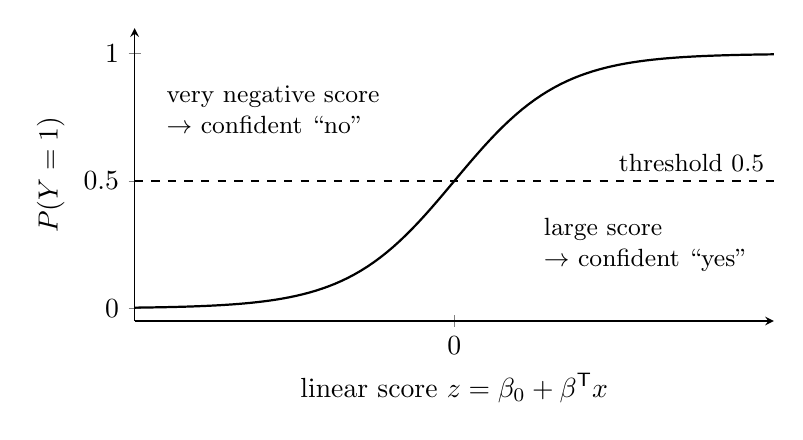
\begin{tikzpicture}
\begin{axis}[
  width=0.80\linewidth, height=5.3cm,
  axis lines=left,
  xlabel={linear score $z=\beta_0+\bm{\beta}^{\mathsf T}\bm{x}$},
  ylabel={$P(Y=1)$},
  ytick={0,0.5,1}, xtick={0},
  domain=-6:6, samples=100, ymin=-0.05, ymax=1.1, clip=false
]
\addplot[thick] {1/(1+exp(-x))};
\draw[dashed] (axis cs:-6,0.5) -- (axis cs:6,0.5)
  node[above left, font=\small] {threshold $0.5$};
\node[font=\small, align=left] at (axis cs:3.6,0.25) {large score\\$\rightarrow$ confident ``yes''};
\node[font=\small, align=left] at (axis cs:-3.4,0.78) {very negative score\\$\rightarrow$ confident ``no''};
\end{axis}
\end{tikzpicture}
\end{utpfig}

A unit increase in $x_j$ multiplies the odds by $e^{\beta_j}$, holding other features fixed. So $\beta_j=0.7$ roughly doubles the odds and $-0.7$ roughly halves them. The effect on the probability depends on where you start, because the curve is steep in the middle and flat at the ends.

\begin{workedexample}
Suppose a pass/fail model based on hours studied has $\beta_0=-4$ and $\beta_1=0.08$.
A student with $x=60$ hours has score $z=-4+0.08\times 60=0.8$ and pass probability $\sigma(0.8)\approx 0.69$.
A student with $x=30$ hours has $z=-1.6$ and $\sigma(-1.6)\approx 0.17$.
Each additional hour multiplies the odds of passing by $e^{0.08}\approx 1.083$ --- about an $8\%$ increase in the odds, regardless of the starting point.
\end{workedexample}

\section{The loss: confident and wrong}

We need to score a probability. Reaching for squared error again seems natural, so try it on a student who failed, with the model giving three different chances of passing.

\begin{workedexample}
\centering\small
\begin{tabular}{@{}lccc@{}}
\toprule
\rowcolor{UTPPaleBlue!92}
\utpth{Chance given to ``pass''} & \utpth{The lean} & \utpth{Squared error} & \utpth{Log-loss fee} \\
\midrule
0.60 & mild & $0.60^2=0.360$ & $-\ln(0.40)=0.916$ \\
0.90 & strong & $0.90^2=0.810$ & $-\ln(0.10)=2.303$ \\
0.99 & certain & $0.99^2=0.980$ & $-\ln(0.01)=4.605$ \\
\bottomrule
\end{tabular}
\par\raggedright
\medskip
Squared error cannot pass 1, so being certain and wrong costs 0.98, barely more than the 0.81 for merely leaning that way. It has run out of room exactly where the mistake is worst. The fee on the right has no ceiling.
\end{workedexample}

The better score is \term{log loss}, also called \term{cross-entropy}: the fee is minus the logarithm of the probability the model gave to what actually happened.
\[
  \mathcal{L}(y,p)
  =-[y\log p+(1-y)\log(1-p)].
\]
A probability is below 1, so its logarithm is negative, and the minus sign turns that into a positive fee. A sure right answer is almost free. A sure wrong answer is ruinous. A model that says 50\% pays 0.693 whichever way the case goes (\figref{fig:fees}).

\begin{utpfig}[The fee for each probability]{The log-loss fee against the chance given to ``pass'', for a student who passed and a student who failed. The two curves cross at 0.5, where the fee is 0.693, and each climbs without limit as the model grows confident and wrong. Squared error for a failing student is shown for comparison.}{fig:fees}
\begin{tikzpicture}
\begin{axis}[logaxis, width=0.70\linewidth, height=5.4cm, xlabel={chance given to ``pass''}, ylabel={fee}, xmin=0, xmax=1, ymin=0, ymax=5,
  legend style={at={(0.5,0.97)},anchor=north}]
\addplot[draw=UTPBlue,thick,domain=0.007:1,samples=80] {-ln(x)}; \addlegendentry{student passed: $-\ln p$}
\addplot[draw=UTPOrange,thick,domain=0:0.993,samples=80] {-ln(1-x)}; \addlegendentry{student failed: $-\ln(1-p)$}
\addplot[draw=UTPMuted,dashed,domain=0:1] {x^2}; \addlegendentry{squared error, student failed}
\end{axis}
\end{tikzpicture}
\end{utpfig}

\section{The optimizer: walking down}

Unlike squared error on a line, log loss has no exact formula for its best $w$ and $b$, so the model has to walk. Everything you need is already here: the model, the loss, and the gradient-descent rule from \secref{sec:gradient-descent}. The two slopes work out neatly: for each row, the slope is simply the prediction minus the truth, $(p_i-y_i)$, weighted by the feature.
\[
  \frac{\partial J}{\partial w}=\frac{1}{n}\sum_i(p_i-y_i)\,x_i,
  \qquad
  \frac{\partial J}{\partial b}=\frac{1}{n}\sum_i(p_i-y_i).
\]
We center the lectures on 8, because that keeps the numbers small. Nothing else changes. The whole fit, in code:

\lstinputlisting[style=utppython,firstline=61,lastline=80]{all_experiments/book_checks/demo_study_log.py}

\begin{workedexample}
At the start, $w=b=0$, so every $p$ is 0.5. The formula gives a slope of $-1.0000$ for $w$. Nudging $w$ by 0.001 and remeasuring the loss gives $-0.9988$, so the formula checks out. With a learning rate of 0.1:

\medskip
\centering\small
\begin{tabular}{@{}cccc@{}}
\toprule
\rowcolor{UTPPaleBlue!92}
\utpth{Step} & \utpth{$w$} & \utpth{$b$} & \utpth{Log loss} \\
\midrule
1 & 0.1000 & 0.0200 & 0.6011 \\
10 & 0.4497 & 0.1612 & 0.4285 \\
100 & 0.6819 & 0.8664 & 0.3528 \\
500 & 0.7827 & 1.3163 & 0.3430 \\
2000 & 0.7885 & 1.3371 & 0.3430 \\
\bottomrule
\end{tabular}
\par\raggedright
\medskip
The loss falls fast and then barely moves, because the walk has reached the flat bottom.
\end{workedexample}

\section{What the fitted model says}

Follow one student all the way through. Student A attended 8 lectures, so the centered value is 0. The score is $0.7885\times0+1.3371=1.337$, and the chance of passing is $\sigma(1.337)=0.792$. The score can be any number at all; the probability can never leave 0 to 1.

\begin{utptable}
\centering
\begin{tabular}{@{}>{\bfseries\color{UTPNavy}}ccccccc@{}}
\toprule
\rowcolor{UTPPaleBlue!92}
\utpth{Student} & \utpth{Lectures} & \utpth{Passed?} & \utpth{Score} & \utpth{Chance} & \utpth{Verdict} & \utpth{Right?} \\
\midrule
J & 3 & no & $-2.605$ & 0.069 & fail & yes \\
I & 5 & no & $-1.028$ & 0.263 & fail & yes \\
B & 6 & yes & $-0.240$ & 0.440 & fail & \textbf{no} \\
C & 7 & yes & 0.549 & 0.634 & pass & yes \\
A & 8 & no & 1.337 & 0.792 & pass & \textbf{no} \\
D & 9 & yes & 2.126 & 0.893 & pass & yes \\
H & 10 & yes & 2.914 & 0.949 & pass & yes \\
E & 11 & yes & 3.703 & 0.976 & pass & yes \\
G & 12 & yes & 4.491 & 0.989 & pass & yes \\
F & 13 & yes & 5.280 & 0.995 & pass & yes \\
\bottomrule
\end{tabular}
\end{utptable}

The model is right on 8 of 10. Its two mistakes differ in kind. Student B was a near thing at 0.44, and pays a fee of 0.820. Student A is the expensive one: the model was 79\% sure, and A failed, for a fee of 1.570. A's two hours of study are not visible to a model that sees only lectures, which is a reminder that a model can be only as good as its columns.

Each extra lecture multiplies the odds of passing by $e^{0.7885}=2.20$. The score is zero, and the chance exactly 0.5, at $8-1.3371/0.7885=6.30$ lectures. That point is the \term{decision boundary}.

\subsection{The decision boundary and the threshold}

At threshold $0.5$, class~1 means $z\ge0$, giving the boundary $\beta_0+\bm{\beta}^{\mathsf T}\bm{x}=0$. With two features that boundary is a straight line, and with more it is a flat plane, which is why logistic regression is called a linear classifier even though its output curve is not straight.

The probability and the decision are separate objects. The model supplies the first. The threshold is a policy, chosen to reflect error costs on validation or out-of-fold predictions (\chapref{ch:evaluation}). These are Lab~2's results for one fitted model on the 40,687 hotel bookings of 2017, Part~C, where a flagged booking is treated as a likely cancellation:

\begin{utptable}
\begin{tabularx}{\linewidth}{@{}>{\bfseries\leavevmode\color{UTPNavy}}m{0.14\linewidth}ccccX@{}}
\toprule
\rowcolor{UTPPaleBlue!92}
\utpth{Threshold} & \utpth{Flagged} & \utpth{Precision} & \utpth{Recall} & \utpth{Cancellations missed} & \utpth{What changed} \\
\midrule
0.30 & 20,052 & 0.61 & 0.77 & 3,558 & many bookings flagged; most cancellations caught \\
0.50 & 11,095 & 0.78 & 0.55 & 7,129 & the default \\
0.70 & 4,822 & 0.96 & 0.29 & 11,117 & few flagged, almost all right; most cancellations missed \\
\bottomrule
\end{tabularx}
\end{utptable}

Choose the operating point from a stated cost or capacity. Then refit on all training data and assess the locked rule on the test set once.

\subsection{Regularization}

Use $L_1$ or $L_2$ penalties with appropriately scaled features and validation-selected strength (\chapref{ch:regression}). Regularization also stops coefficients diverging on perfectly separable data, where a steeper S always scores better and the walk would never end. Lab~2's grid search tunes this strength as $C$, and in scikit-learn a larger $C$ means a weaker penalty.

\recipecard{Logistic regression}{The straight line's score, squashed by the sigmoid into a probability.}{Log loss, which is very large when the model is confident and wrong.}{Gradient descent or a Newton-type method. No exact formula exists.}

\section{Softmax regression for multiple classes}

For $K$ classes, each class $k$ receives its own weight vector, and the \term{softmax} function converts the $K$ linear scores into probabilities:
\[
  P(Y=k\given\bm{x})
  =\frac{\exp(\bm{\beta}_k^{\mathsf T}\bm{x})}
        {\sum_{j=1}^{K}\exp(\bm{\beta}_j^{\mathsf T}\bm{x})}.
\]
Exponentiating and normalizing preserves score order and makes probabilities sum to one. Training minimizes $\mathcal{L}=-\log P(Y=y\given\bm{x})$.

\term{One-vs-rest} trains $K$ binary classifiers, one class against all others, and predicts the highest-scoring class.

\begin{utpfig}[Softmax]{Softmax turns class scores into probabilities. Scores 1.2, 3.4 and 2.0 become 0.08, 0.74 and 0.18: the order is preserved and the probabilities add to one.}{fig:softmax}
\begin{tikzpicture}[
  node distance=0.36cm and 0.62cm,
  sc/.style={draw=UTPBlue,fill=UTPPaleBlue,rounded corners=1.2mm,minimum width=1.55cm,minimum height=0.6cm,align=center,font=\scriptsize\color{UTPNavy}},
  pr/.style={draw=UTPGreen,fill=UTPPaleTeal,rounded corners=1.2mm,minimum width=1.55cm,minimum height=0.6cm,align=center,font=\scriptsize\color{UTPNavy}},
  arr/.style={-{Stealth[length=2mm]},thick,draw=UTPTeal}
]
\node[sc] (s1) {cat: $1.2$};
\node[sc,below=of s1] (s2) {dog: $3.4$};
\node[sc,below=of s2] (s3) {fox: $2.0$};
\node[draw=UTPOrange,fill=UTPPaleOrange,rounded corners=2mm,minimum height=2.5cm,minimum width=1.9cm,align=center,font=\scriptsize\bfseries\color{UTPNavy},right=1.0cm of s2] (sm) {softmax\\[0.15em]\scriptsize\mdseries exponentiate,\\then divide by\\the total};
\node[pr,right=1.0cm of sm] (p2) {dog: $0.74$};
\node[pr,above=of p2] (p1) {cat: $0.08$};
\node[pr,below=of p2] (p3) {fox: $0.18$};
\draw[arr] (s1.east) -- (sm.west); \draw[arr] (s2.east) -- (sm.west); \draw[arr] (s3.east) -- (sm.west);
\draw[arr] (sm.east) -- (p1.west); \draw[arr] (sm.east) -- (p2.west); \draw[arr] (sm.east) -- (p3.west);
\node[font=\scriptsize\itshape\color{UTPMuted},below=0.3cm of p3] {always adds to 1.00};
\end{tikzpicture}
\end{utpfig}

\begin{workedexample}
For scores $1.2,\ 3.4,\ 2.0$, the exponentials are $3.32,\ 29.96,\ 7.39$, which add to $40.67$. Dividing gives $0.082,\ 0.737,\ 0.182$.
\end{workedexample}

\begin{keyidea}
Softmax preserves score order while normalizing exponentials to a probability distribution.
\end{keyidea}

\section{Ordered categories are not ordinary multiclass labels}
\label{sec:ordinal-labels}

\term{Ordinal labels} have order, such as low $<$ medium $<$ high. Softmax ignores order; numerical coding for regression assumes meaningful gaps.

\begin{utptable}
\begin{tabularx}{\linewidth}{@{}m{0.25\linewidth}X@{}}
\toprule
\rowcolor{UTPPaleBlue!92}
\utpth{Approach} & \utpth{When it makes sense} \\
\midrule
Ordinary multiclass classifier & Use when categories are genuinely unordered or when order is irrelevant to the decision. \\
Ordinal model / order-aware loss & Prefer when confusing adjacent levels is meaningfully less serious than confusing the two extremes. \\
Regression on integer codes & Use only when the numerical spacing itself is defensible; do not use it merely because the labels can be numbered. \\
\bottomrule
\end{tabularx}
\end{utptable}

Choose order-aware methods or metrics when warranted, and validate whether they help.

\section{Linear discriminant analysis}

Logistic regression learns the boundary directly. Another way to classify is to describe each class by itself, and then ask which description fits a new row better.

Logistic regression is \term{discriminative}: it models $P(y\given\bm{x})$. \term{Linear discriminant analysis (LDA)} is \term{generative}: it models each class's feature distribution and applies Bayes' theorem.

LDA assumes Gaussian classes with means $\bm\mu_k$, shared covariance $\Sigma$, and priors $\pi_k$. Choose the largest discriminant score:
\[
  \delta_k(\bm{x})
  =\bm{x}^{\mathsf T}\Sigma^{-1}\bm{\mu}_k
  -\tfrac{1}{2}\bm{\mu}_k^{\mathsf T}\Sigma^{-1}\bm{\mu}_k
  +\log\pi_k.
\]
Estimate priors from frequencies, means within classes, and covariance from pooled within-class variation. Linear dependence on $\bm x$ gives flat boundaries.

\begin{workedexample}
On the lectures column of the log, passing students average 9.71 lectures and failing students 5.33, with a pooled variance of 6.51. With equal class sizes the boundary would be the midpoint, 7.52. Passing is more common here (7 of 10), and the prior moves the boundary down to 6.26, close to logistic regression's 6.30.
\end{workedexample}

\begin{intuition}
With equal-shaped Gaussian class densities, the tie boundary is linear; class priors shift its position.
\end{intuition}

When to prefer which:

\begin{itemize}
  \item LDA can be stable on small datasets when Gaussian assumptions are reasonable.
  \item Logistic regression assumes less about the features and is more robust when classes are far from Gaussian (heavy tails, strong outliers, many binary features).
  \item LDA also finds up to $K-1$ supervised projection directions for $K$ classes (\chapref{ch:dimred}).
\end{itemize}

\term{Quadratic discriminant analysis (QDA)} drops the shared-covariance assumption and gives each class its own $\Sigma_k$. The boundaries become curved (quadratic), which is more flexible but requires estimating many more parameters --- QDA needs considerably more data per class to stay reliable.

\section{The perceptron}

The perceptron is the simplest trainer there is, and the ancestor of the neural networks in \chapref{ch:deep}. It has no probabilities and no loss curve: when it makes a mistake it moves the line, and when it does not, it does nothing.

The \term{perceptron} predicts $\hat y=\operatorname{sign}(\bm w^{\mathsf T}\bm x+b)$ for $y\in\{-1,+1\}$. For each misclassified example, update
\[
  \bm{w}\leftarrow\bm{w}+\eta\,y_i\,\bm{x}_i,
  \qquad
  b\leftarrow b+\eta\,y_i.
\]
Correct predictions cause no update. Separable data yields convergence; otherwise convergence is not guaranteed. The boundary depends on the training path and supplies no probabilities.

\begin{workedexample}
Four points: $(2,2)$ and $(0,2)$ are $+1$; $(-1,-1)$ and $(1,-1)$ are $-1$. Start with $\bm{w}=(0,0)$, $b=0$ and $\eta=1$.
\begin{description}
  \item[$(2,2)$] The score is 0, which counts as a mistake, so $\bm{w}=(2,2)$ and $b=1$.
  \item[$(-1,-1)$] The score is $-3$, which is correct, so nothing changes.
  \item[$(1,-1)$] The score is $+1$, a mistake, so $\bm{w}=(1,3)$ and $b=0$.
  \item[$(0,2)$] The score is $+6$, which is correct.
\end{description}
A second pass makes no mistakes, so training stops with $\bm{w}=(1,3)$ and $b=0$.
\end{workedexample}

\section{Choosing among linear classifiers}

\begin{utptable}
\begin{tabular}{@{}p{0.22\linewidth}p{0.34\linewidth}p{0.34\linewidth}@{}}
\toprule
\rowcolor{UTPPaleBlue!92}
\utpth{Model} & \utpth{Useful strengths} & \utpth{Important limitations} \\
\midrule
Logistic regression & Strong probability baseline, convex training, interpretable odds ratios & Linear boundary; probabilities can still be miscalibrated under misspecification or shift \\
LDA & Very fast, stable on small data, gives class-separating directions & Assumes Gaussian classes with shared covariance \\
QDA & Curved boundaries, per-class covariance & Many parameters; needs much more data \\
Perceptron & Simplest possible trainer; historically important & No probabilities; unreliable when classes overlap \\
\bottomrule
\end{tabular}
\end{utptable}

\begin{keyidea}
Logistic regression fits conditional probabilities; LDA models class distributions; the perceptron updates after mistakes. All use flat boundaries, while QDA's separate covariance matrices allow curves.
\end{keyidea}

\begin{modelcard}{Linear Classifiers - Quick Guide}
\begin{tabularx}{\linewidth}{@{}>{\bfseries\leavevmode\color{UTPNavy}}p{0.24\linewidth}X@{}}
Best when & A linear boundary is reasonable, fast prediction matters, or coefficients need to be interpreted. \cr
Start with & Logistic regression for probabilities; softmax regression for several classes. \cr
Preprocessing & Encode categories, standardize numerical features for regularization, and handle imbalance with suitable metrics or weights. \cr
Main controls & Regularization strength, penalty type, and the probability threshold used for decisions. \cr
Watch for & Nonlinear class structure, poorly calibrated probabilities, rare classes, and causal over-interpretation (\secref{sec:correlation}). \cr
\end{tabularx}
\end{modelcard}

\begin{workedexample}
For an ``hours studied'' coefficient of $0.62$, each extra hour multiplies passing odds by $e^{0.62}\approx1.86$, holding other features fixed. The probability increase depends on the starting probability.
\end{workedexample}

\begin{tryit}
Fit logistic regression and obtain out-of-fold training probabilities. Sweep thresholds from 0.05 to 0.95 in steps of 0.05; plot precision against recall without using test data.
\end{tryit}

\begin{debugtask}
A teammate lowers the probability threshold until test-set recall reaches the desired value, then reports that same test recall as final performance. Explain the leakage in model selection and show where threshold tuning belongs instead.
\end{debugtask}

\begin{decisionmemo}
For a rare positive class, choose between an unweighted logistic model, class weighting, and a lower decision threshold. State which quantity each intervention changes, which validation metric you would inspect, and why the three options are not interchangeable.
\end{decisionmemo}

\begin{chapterrecap}
\begin{itemize}
  \item A straight line on 0/1 labels leaves the range of a probability, so logistic regression passes its score through the sigmoid, a dimmer that stops at 0 and 1.
  \item The score's sign picks the side and its size sets the confidence. A unit of a feature multiplies the odds by $e^{\beta}$.
  \item Log loss charges minus the log of the probability given to what happened, so confident and wrong is ruinous. Squared error cannot punish it enough.
  \item There is no formula, so the model walks down by gradient descent. Each row's slope is the prediction minus the truth, weighted by the feature.
  \item The probability and the threshold are separate. Softmax extends the model to many classes; LDA models each class; the perceptron just corrects its mistakes.
\end{itemize}
\end{chapterrecap}

\begin{quickcheck}
\begin{enumerate}
  \item A score is exactly 0. What probability does the sigmoid give, and why?
  \item With the fitted model, what chance of passing does a student with 7 lectures get, and which side of a 0.5 threshold is that?
  \item A model gives 0.95 to a case that turns out negative. What does it pay in log loss? And for a case that turns out positive?
  \item Why is logistic regression called a linear classifier even though it outputs a nonlinear sigmoid probability?
  \item Why should the probability model and the operational classification threshold be treated as separate objects?
  \item What changes when binary logistic regression is extended to a multiclass softmax model?
\end{enumerate}
\end{quickcheck}

\begin{checkanswers}
\begin{enumerate}
  \item 0.5, because $e^0=1$, so $1/(1+1)=0.5$. The two limits, 0 and 1, are approached but never reached.
  \item 0.634, from a score of 0.549. That is above 0.5, so the verdict is pass, and student C did pass.
  \item Negative case: $-\ln(0.05)=3.00$. Positive case: $-\ln(0.95)=0.05$.
  \item The decision boundary, where the score equals zero, is a flat line or plane in feature space. The sigmoid only maps the score to a probability, and it does not bend the boundary.
  \item The fitted model describes how likely each outcome is, which stays the same however it is used. The threshold is a choice about costs and capacity, which can change without refitting.
  \item Each class gets its own weight vector and score, and softmax turns the scores into probabilities that add to one. Binary logistic regression is the two-class special case.
\end{enumerate}
\end{checkanswers}

\labsection{2}{Supervised learning I: regression, classification, and the workflow}{sec:lab02-supervised-workflow}

\begin{labproject}{A regression problem, two classification problems, and saved models at the end}
\textbf{Read first.} Chapters~\ref{ch:learning}--\ref{ch:classification}.\\
\textbf{Goal.} Fit regression and classification pipelines on messy data, validate in date order where time matters, choose thresholds and hyperparameters on purpose, test once, and save models that can be loaded and used.\\
\textbf{Scenario.} Three commissions: a used-car dealer wants asking prices estimated from a listing, a hotel group wants to know which bookings will be cancelled so it can resell rooms without turning guests away, and a telecom company wants a churn model it can hand to its call centre. Then the models must leave the notebook as files.\\
\textbf{Data.} In \texttt{all\_datasets/\allowbreak supervised/}: \texttt{used\_cars/\allowbreak used\_cars.zip}, 150,000 car listings collected from Cars.com in October 2026; \texttt{hotel\_bookings/\allowbreak hotel\_bookings.zip}, the hotel bookings from Lab~1; and \texttt{telco\_customer\_churn/\allowbreak telco\_customer\_churn.csv}, the telecom customers from Lab~1. Each folder's \texttt{README.md} is its data card.\\
\textbf{Notebook.} \texttt{all\_experiments/\allowbreak lab02\_supervised\_workflow/\allowbreak lab02\_supervised\_workflow\_worked.ipynb}, with \texttt{predict\_churn.py} and a README beside it.\\
\textbf{Hand in.} The executed notebook, \texttt{results/lab02/}, the model files and a decision memo, as listed in the checklist at the end of this sheet.
\end{labproject}

\labroadmap{Your map of this lab}{
      A & Tidy the car listings, predict prices, read the coefficients and the residuals & 2--5 \\
      B & Validate hotel cancellations in date order, and see what a shuffled split hides & 6--8 \\
      C & Beat a baseline, read probabilities, and choose a threshold by cost & 9--12 \\
      D & Tune the churn model with cross-validation, then open the test set once & 13--14 \\
      E & Save the models with a card, reload them and use them & 15--16 \\
      Finish & Save the evidence; then model log prices and write an overbooking memo & 17--19 \\
      After & Your-turn tasks, expected findings, troubleshooting and the two checklists & --- \\
}

\begin{labmode}
\begin{enumerate}
  \item Activate your course environment and confirm the three data files are in \texttt{all\_datasets/\allowbreak supervised/}.
  \item From the course folder, start Jupyter, open the notebook, and choose \textbf{Restart Kernel and Run All Cells}. It takes under a minute.
\end{enumerate}
\begin{lstlisting}[style=utpterminal]
jupyter lab
\end{lstlisting}
Prefer a plain script? From the course folder, \texttt{python all\_experiments/\allowbreak lab02\_supervised\_workflow/\allowbreak lab02\_supervised\_workflow\_worked.py} runs the same code and writes the same evidence.
\end{labmode}

\labroutine

\begin{yourturn}
\textbf{Warm-up on paper.} Do these before opening the notebook; the code will check you.
\begin{enumerate}
  \item True values $10,20,30,40$ and predictions $12,18,30,50$. Compute MAE and RMSE. Why is RMSE larger? (MAE 3.5, RMSE about 5.2.)
  \item Question~9's logistic model at threshold 0.50 flags 2017 bookings as likely cancellations with $TP=8{,}616$, $FP=2{,}479$, $FN=7{,}129$ and $TN=22{,}463$. Compute precision, recall and accuracy. Then predict: if the threshold rises to 0.70, which of these four counts can only grow, and which can only shrink?
\end{enumerate}
\end{yourturn}

\begin{labquestion}{1}{Setup}
Run this first, and keep this kernel for the later questions. Every lab starts the same way. \texttt{start\_lab()}, from \texttt{all\_experiments/\allowbreak course\_setup.py}, finds the course folder and returns the three folders the lab uses: \texttt{DATA} to read from, \texttt{RESULTS} and \texttt{MODELS} to write to. The imports in between are grouped by what they are for. \texttt{make\_preprocess} is the same helper as in Lab~1: median imputation and scaling for numbers, most-frequent imputation and one-hot encoding for categories.
\end{labquestion}
\begin{labanswer}
\lstinputlisting[style=utppython,firstline=11,lastline=51]{all_experiments/lab02_supervised_workflow/lab02_supervised_workflow_worked.py}
\begin{refoutput}
\begin{lstlisting}[style=utpterminal]
course folder: MACHINE LEARNING
reads all_datasets/, writes results/lab02/ and models/
\end{lstlisting}
\end{refoutput}
\end{labanswer}

\labpartopen{Part A}{Regression: ordinary least squares versus ridge}{Questions 2--5 \textbullet\ Data: used-car listings from Cars.com}{Tidy real listings, predict used-car prices with a straight-line model, read its coefficients, and see where it fails.}

\begin{labquestion}{2}{Read the car listings, tidy them, and split}
Each row is one car with a numeric label, \texttt{price\_usd}, so this is regression. Three fixed rules, chosen before any model, keep used cars with a believable price (\$1,000 to \$200,000) and a real odometer reading. Sellers also type the same thing many ways, so \texttt{tidy()} maps the spellings of drivetrain and fuel to a few groups. Two models will share the pipeline and the split; the only difference is ridge's penalty on large coefficients. The car's \texttt{model} (F-150, Camry and over a thousand others) is kept aside for now, and a Your-turn task brings it in.
\end{labquestion}
\begin{labanswer}
\lstinputlisting[style=utppython,firstline=53,lastline=87]{all_experiments/lab02_supervised_workflow/lab02_supervised_workflow_worked.py}
\begin{refoutput}
\begin{lstlisting}[style=utpterminal]
shape: (150000, 19)
stock_type
Used    79262
New     70738
used listings kept: 77,646 of 79,262
spellings before tidying: drivetrain 21  fuel 31
{'AWD': 28787, 'FWD': 18290, '4WD': 17310, 'RWD': 9008, None: 4251}
{'gasoline': 63296, None: 5474, 'electric': 3007, 'hybrid': 2986, 'diesel': 2160,
 'flex fuel': 594, 'plug-in hybrid': 129}
62116 listings to train on and 15530 to validate
\end{lstlisting}
\end{refoutput}

\textbf{What it means.} The rules drop 1,616 used listings, among them 295 with no price shown, 712 priced above \$200,000 (24 of them in the millions) and 659 with 100 miles or fewer on the clock; a few break two rules. Tidying turns 21 spellings of the drivetrain and 31 of the fuel into four and six groups; what matches no group (``2WD'', ``Unknown'', a blank) becomes a gap that the pipeline's imputer fills. Every rule is fixed and reads no label, so it may run before the split. The listings were collected on one day, so a random 80/20 split is honest here.
\end{labanswer}

\begin{labquestion}{3}{Fit OLS and ridge}
Three scores per model. MAE is the typical miss in dollars. RMSE weights big misses more, so when it is much larger than MAE a few predictions are badly wrong. $R^2$ is the share of the price's variation the model explains. Always guessing the training mean is the baseline both must beat.
\end{labquestion}
\begin{labanswer}
\lstinputlisting[style=utppython,firstline=89,lastline=107]{all_experiments/lab02_supervised_workflow/lab02_supervised_workflow_worked.py}
\begin{refoutput}
\begin{lstlisting}[style=utpterminal]
always the training mean: MAE 15408

linear regression          ridge
MAE: 9009                  MAE: 9062
RMSE: 14336                RMSE: 14427
R2: 0.575                  R2: 0.569
\end{lstlisting}
\end{refoutput}

\textbf{What it means.} Both models cut the typical miss from \$15,400 to about \$9,000, and regularization did not help: with 62,116 rows the plain model is already stable. RMSE is about 60\% above MAE, so some cars are missed by far more than the typical amount; Question~5 shows which.
\end{labanswer}

\begin{labquestion}{4}{Read the coefficients}
A linear model is readable: each coefficient is the change in predicted price for a one-unit change in that feature, the others held fixed. The two numeric columns were standardized, so one unit is one standard deviation. Every make gets its own one-hot coefficient, and the cell counts the training listings behind each one.
\end{labquestion}
\begin{labanswer}
\lstinputlisting[style=utppython,firstline=109,lastline=132]{all_experiments/lab02_supervised_workflow/lab02_supervised_workflow_worked.py}
\begin{refoutput}
\begin{lstlisting}[style=utpterminal]
one standard deviation: {'age': 5.6, 'mileage_miles': 47396.4}
num__age             -3302.0
num__mileage_miles   -8553.0
the four largest:
              coefficient  listings
McLaren          76900.0        16
Ferrari          82800.0        18
Lancia           83000.0         1
Lamborghini     115700.0        14
30 makes have 500 listings or more, for example: {'Porsche': 26300.0, 'Toyota': -11600.0,
 'Ford': -13100.0, 'Mitsubishi': -26800.0}
\end{lstlisting}
\end{refoutput}

\textbf{What it means.} One standard deviation of mileage, about 47,000 miles, takes \$8,553 off the price, and one of age, 5.6 years, another \$3,302. Age matters less than you might expect partly because the two move together (correlation 0.61): an old car usually has high mileage, and the model credits much of the wear to the odometer. The make coefficients are read as differences: a Porsche is priced \$37,900 above an otherwise identical Toyota, and a Mitsubishi \$15,200 below. The largest coefficients belong to supercars, and Lancia's rests on a single listing: a rare category gets a confident-looking number from almost no evidence. Each coefficient is an association inside this model, not a cause.
\end{labanswer}

\begin{labquestion}{5}{Plot the residuals}
Two diagnostic plots for the ridge model. A good residual plot is a shapeless band around zero; any shape is something the model failed to use.
\end{labquestion}
\begin{labanswer}
\courselabtrace{Trace prediction and regression scoring}{1. Input / state}{The validation rows provide y\_valid; each fitted pipeline produces predictions in the original charges units.}{2. Operation}{The model loop computes MAE, RMSE and R-squared from the same actual/predicted pairs.}{3. Check}{Store each model's predictions and inspect residual = y\_valid - ridge\_pred.}

\lstinputlisting[style=utppython,firstline=134,lastline=158]{all_experiments/lab02_supervised_workflow/lab02_supervised_workflow_worked.py}
\begin{refoutput}
\begin{lstlisting}[style=utpterminal]
spread of the residuals (standard deviation) by quarter of predicted price:
cheapest     9172.0
second       8125.0
third       10943.0
dearest     23079.0
predicted prices below zero: 377
\end{lstlisting}
\end{refoutput}

\textbf{What it means.} The residuals fan out: a typical miss of \$8,000 to \$9,000 on the cheaper half of the predictions grows to \$23,079 on the dearest quarter, and 377 cars get a negative price. One straight surface cannot serve a \$5,000 hatchback and a \$150,000 sports car equally well, because a car loses value in proportions, not in fixed dollars. The Try-it fixes the shape; Your-turn task~1 adds the idea the model is missing.
\end{labanswer}

\begin{labcheckpoint}
\begin{itemize}[leftmargin=1.2em,itemsep=2pt,topsep=1pt]
  \item Linear regression misses by \$9,009 on average, against \$15,408 for always guessing the mean; ridge is no better.
  \item The residual spread grows to \$23,079 on the dearest quarter of predictions, and 377 cars get a negative price.
\end{itemize}
\end{labcheckpoint}

\labpartopen{Part B}{Classification in time: validate in date order}{Questions 6--8 \textbullet\ Data: hotel bookings}{Validate a cancellation model the way a hotel would use it: train on past arrivals, score future ones.}

\begin{labquestion}{6}{Split the bookings in date order}
Lab~1 scored its hotel model on a shuffled split. A hotel, though, always predicts bookings for dates that have not happened yet, from bookings that already have. So the rows are sorted by arrival date, Lab~1's five engineered columns are rebuilt, and arrivals up to the end of 2016 train while the eight months of 2017 validate.
\end{labquestion}
\begin{labanswer}
\lstinputlisting[style=utppython,firstline=160,lastline=187]{all_experiments/lab02_supervised_workflow/lab02_supervised_workflow_worked.py}
\begin{refoutput}
\begin{lstlisting}[style=utpterminal]
train: 2015-07-01 to 2016-12-31, 78,703 bookings, 36.2% cancelled
valid: 2017-01-01 to 2017-08-31, 40,687 bookings, 38.7% cancelled
\end{lstlisting}
\end{refoutput}

\textbf{What it means.} Two thirds of the bookings train and one third validate, and the cancellation rate is already higher in the later period. \texttt{reservation\_status} stays out, as Lab~1 showed it must.
\end{labanswer}

\begin{labquestion}{7}{Score one model on two splits}
The same logistic regression as Lab~1, fitted twice: once on a shuffled 75/25 split, once on the date split. Only the split differs, so any gap between the two scores is what the shuffle was hiding.
\end{labquestion}
\begin{labanswer}
\lstinputlisting[style=utppython,firstline=189,lastline=200]{all_experiments/lab02_supervised_workflow/lab02_supervised_workflow_worked.py}
\begin{refoutput}
\begin{lstlisting}[style=utpterminal]
shuffled split, ROC AUC:     0.858
date split (2017), ROC AUC:  0.824
\end{lstlisting}
\end{refoutput}

\textbf{What it means.} The shuffled split flatters the model by more than three points. It let the model train on bookings from the very weeks it was tested on, which a hotel can never do. Your-turn task~2 finds a second reason: thousands of bookings in this file have exact twins.
\end{labanswer}

\begin{labquestion}{8}{Compare the months}
Averaging the predicted probabilities over each month of arrival gives the share of bookings the model expected to cancel; the actual share sits beside it. Months before 2017 were seen in training, and the months after were not.
\end{labquestion}
\begin{labanswer}
\lstinputlisting[style=utppython,firstline=202,lastline=218]{all_experiments/lab02_supervised_workflow/lab02_supervised_workflow_worked.py}
\begin{refoutput}
\begin{lstlisting}[style=utpterminal]
arrival_date  2016-12  2017-01  2017-02  2017-03  2017-04  2017-05  2017-06  2017-07  2017-08
actual          0.362    0.340    0.325    0.336    0.435    0.438    0.432    0.373    0.369
predicted       0.296    0.303    0.291    0.346    0.406    0.412    0.420    0.361    0.346
\end{lstlisting}
\end{refoutput}

\textbf{What it means.} The model follows the training months closely, then under-predicts most of 2017: 30.3\% expected in January against 34.0\%, and about 41\% in April to June against 43 to 44\%. Its ranking still works, but the world it learned from had moved on, and only a split in date order shows it. Lab~8 forecasts a series from its own past, where the same rule holds.
\end{labanswer}

\begin{labcheckpoint}
\begin{itemize}[leftmargin=1.2em,itemsep=2pt,topsep=1pt]
  \item Training arrivals end on 31 December 2016; the 40,687 arrivals of 2017 are the validation set.
  \item The same model scores ROC AUC 0.858 shuffled and 0.824 in date order.
\end{itemize}
\end{labcheckpoint}

\labpartopen{Part C}{Classification: baselines, probabilities, and the threshold}{Questions 9--12 \textbullet\ Data: hotel bookings, split in date order}{Beat a baseline, read predicted probabilities, and choose a threshold by what each error costs.}

\begin{labquestion}{9}{Set a baseline and compare classifiers on 2017}
The date split from Part~B, and two classifiers with the same preparation. Logistic regression is the simple, readable reference, and a random forest the more flexible challenger. Accuracy counts correct decisions at the default 0.5 cutoff; ROC AUC judges how well a model ranks bookings, independent of any cutoff. A hotel would act on a flagged booking by reselling its room, so precision asks: when the model says a booking will cancel, how often is it right?
\end{labquestion}
\begin{labanswer}
\lstinputlisting[style=utppython,firstline=220,lastline=249]{all_experiments/lab02_supervised_workflow/lab02_supervised_workflow_worked.py}
\begin{refoutput}
\begin{lstlisting}[style=utpterminal]
majority-class baseline accuracy: 0.613
logistic       accuracy=0.764 roc_auc=0.824
random_forest  accuracy=0.770 roc_auc=0.841
threshold 0.30: precision=0.61 recall=0.77
threshold 0.50: precision=0.78 recall=0.55
threshold 0.70: precision=0.96 recall=0.29
\end{lstlisting}
\end{refoutput}

\textbf{What it means.} Both models clear the baseline, and the forest leads by about two points of ROC AUC. With 40,687 validation bookings that gap is real, but both are scored on one period, and Your-turn task~2 shows how much the forest's lead depends on the split. The threshold table is the same logistic model with three decision rules.
\end{labanswer}

\begin{labquestion}{10}{Plot the cancellation probabilities}
The logistic model gives every 2017 booking a probability of cancelling. Plot those probabilities separately for the bookings that were kept and those that were cancelled: a threshold is a vertical line, and every booking to its right is treated as a likely cancellation whose room can be resold.
\end{labquestion}
\begin{labanswer}
\lstinputlisting[style=utppython,firstline=251,lastline=266]{all_experiments/lab02_supervised_workflow/lab02_supervised_workflow_worked.py}
\begin{refoutput}
\begin{lstlisting}[style=utpterminal]
share of 2017 bookings scored between 0.3 and 0.7: 0.374
\end{lstlisting}
\end{refoutput}

\textbf{What it means.} The two groups overlap heavily: more than a third of the bookings sit in the uncertain middle, so wherever the line goes it cuts through both. One feature stands out, a tower of cancelled bookings near 1.0. These are the 4,126 non-refundable bookings of 2017, 99.8\% of which were cancelled, the puzzling pattern the data card warns about.
\end{labanswer}

\begin{labquestion}{11}{Count errors at two thresholds}
The confusion matrix counts what happens on each side of the line: rows are the truth, columns are the decision. Precision asks how often a flagged booking really cancelled; recall asks how many of the cancellations were flagged.
\end{labquestion}
\begin{labanswer}
\lstinputlisting[style=utppython,firstline=268,lastline=277]{all_experiments/lab02_supervised_workflow/lab02_supervised_workflow_worked.py}
\begin{refoutput}
\begin{lstlisting}[style=utpterminal]
threshold = 0.50
[[22463  2479]
 [ 7129  8616]]
           1      0.777     0.547     0.642     15745
threshold = 0.70
[[24748   194]
 [11117  4628]]
           1      0.960     0.294     0.450     15745
\end{lstlisting}
\end{refoutput}

\textbf{What it means.} At 0.50 the hotel flags 11,095 bookings and is right about 8,616 of them, but 2,479 flagged guests arrive to find their room resold. At 0.70 only 194 do, at the price of catching just 4,628 of the 15,745 cancellations and leaving the other rooms empty. Neither number is ``the'' answer: the default 0.50 quietly decides that a walked guest costs no more than an empty room.
\end{labanswer}

\begin{labquestion}{12}{Summarize the ranking: ROC and PR}
Two numbers summarize the ranking without choosing any threshold. ROC AUC is the chance that a random cancelled booking scores higher than a random kept one. Average precision (PR AUC) focuses on the positive class; guessing scores the positive rate, so it is the more honest number when positives are rare.
\end{labquestion}
\begin{labanswer}
\lstinputlisting[style=utppython,firstline=279,lastline=310]{all_experiments/lab02_supervised_workflow/lab02_supervised_workflow_worked.py}
\begin{refoutput}
\begin{lstlisting}[style=utpterminal]
ROC AUC: 0.824
PR AUC (average precision): 0.786  against 0.387 for guessing
\end{lstlisting}
\end{refoutput}

\textbf{What it means.} The ranking is useful but far from perfect: a cancelled booking outranks a kept one about eight times in ten, and average precision doubles the guessing rate. With 38.7\% positives the two summaries tell a similar story; in Lab~5, with 0.17\% frauds, they will not.
\end{labanswer}

\textbf{Connect it to the chapter.} A loss decides what ``wrong'' costs during fitting, and the threshold decides what it costs afterwards.
% Reused from chapters/05-how-supervised-learning-works.tex
\begin{labvisual}{Recall the chapter model}
\begin{labgraphic}
\begin{tikzpicture}[baseline=(current bounding box.north)]
\begin{axis}[
  width=0.45\linewidth, height=4.8cm, axis lines=left,
  title style={font=\small\bfseries\color{UTPNavy},yshift=4pt}, title={Regression losses},
  xlabel={Error $(y-\hat y)$}, ylabel={Penalty},
  label style={font=\scriptsize\color{UTPMuted}}, tick label style={font=\scriptsize\color{UTPMuted}},
  legend style={font=\scriptsize,draw=none,fill=white,fill opacity=0.88,
                text opacity=1,rounded corners=1pt,inner sep=2pt,
                at={(0.5,0.94)},anchor=north,legend columns=3,
                /tikz/every even column/.append style={column sep=0.7em}},
  domain=-3:3, samples=101, xmin=-3, xmax=3, ymin=0, ymax=6.5,
  ytick={0,2,4,6}
]
\addplot[UTPBlue,very thick]{x^2};              \addlegendentry{squared}
\addplot[UTPTeal,very thick]{abs(x)};           \addlegendentry{absolute}
\addplot[UTPOrange,very thick,dashed]{abs(x)<1 ? 0.5*x^2 : abs(x)-0.5}; \addlegendentry{Huber}
\end{axis}
\end{tikzpicture}
\end{labgraphic}\end{labvisual}


\begin{labcheckpoint}
\begin{itemize}[leftmargin=1.2em,itemsep=2pt,topsep=1pt]
  \item On 2017, the majority baseline scores 0.613; logistic regression 0.764 accuracy and 0.824 ROC AUC.
  \item At a threshold of 0.50, 2,479 flagged bookings are kept; at 0.70, only 194 are.
  \item ROC AUC 0.824, and average precision 0.786 against 0.387 for guessing.
\end{itemize}
\end{labcheckpoint}

\labpartopen{Part D}{Tune with cross-validation, then test once}{Questions 13--14 \textbullet\ Data: Telco customer churn}{Choose settings by cross-validation on the training rows, then open the test set exactly once.}

\begin{labquestion}{13}{Tune with cross-validation}
Back to Lab~1's telecom customers, now to predict who leaves (\texttt{Churn}). The column lists come from the data types, and a quarter of the customers is set aside as the \emph{test} set before anything is fitted, so no step of the search can see them. Inside the training rows, five-fold cross-validation scores every combination of \texttt{C} (regularization strength) and \texttt{class\_weight}, and the grid search then refits the winning combination on all training rows.
\end{labquestion}
\begin{labanswer}
\lstinputlisting[style=utppython,firstline=312,lastline=353]{all_experiments/lab02_supervised_workflow/lab02_supervised_workflow_worked.py}
\begin{refoutput}
\begin{lstlisting}[style=utpterminal]
4 numeric and 15 text columns; 26.5% of customers left
cross-validated ROC AUC ranges from 0.841 to 0.844 ; typical fold-to-fold spread 0.015
\end{lstlisting}
\end{refoutput}

\textbf{What it means.} The curve is flat: every setting lies between 0.841 and 0.844, while the error bars, one standard deviation across five folds, are about 0.015. This table does not care much about \texttt{C}, so small gaps between settings should not be over-read.
\end{labanswer}

\begin{labquestion}{14}{Open the test set once}
Only now is the test set touched, once.
\end{labquestion}
\begin{labanswer}
\lstinputlisting[style=utppython,firstline=355,lastline=361]{all_experiments/lab02_supervised_workflow/lab02_supervised_workflow_worked.py}
\begin{refoutput}
\begin{lstlisting}[style=utpterminal]
best parameters: {'model__C': 10.0, 'model__class_weight': None}
cross-validated ROC AUC: 0.844
final test ROC AUC: 0.846 on 1761 customers
\end{lstlisting}
\end{refoutput}

\textbf{What it means.} The test score agrees with the cross-validated one, as it should when the test rows were sealed from the start. It is still one draw: 1,761 customers carry an uncertainty of about a point either way, which Your-turn task~4 measures. Report the test number once, and do not tune again after seeing it.
\end{labanswer}

\courselabtrace{Keep the test set closed}{Training}{Fit preprocessing and candidate models}{Validation}{Compare settings inside training folds}{Holdout}{One final evaluation; save the full pipeline}


\begin{labcheckpoint}
\begin{itemize}[leftmargin=1.2em,itemsep=2pt,topsep=1pt]
  \item Best setting: \texttt{C} = 10 without class weights, cross-validated ROC AUC 0.844.
  \item The final test ROC AUC, 0.846, is reported once, and nothing is tuned after it.
\end{itemize}
\end{labcheckpoint}

\labpartopen{Part E}{Save the models and use them}{Questions 15--16 \textbullet\ Data: the two fitted models}{Save each model with a card, reload it, and use it from a script.}

\begin{labquestion}{15}{Save the churn model with a card}
A model that exists only inside a running notebook is not finished. \texttt{joblib.dump} writes the whole pipeline, preprocessing and estimator together, to one file. A model card written next to it records what the file expects, how well it did, and a typical customer whose values a script can use for any column it is not given.
\end{labquestion}
\begin{labanswer}
\lstinputlisting[style=utppython,firstline=363,lastline=384]{all_experiments/lab02_supervised_workflow/lab02_supervised_workflow_worked.py}
\begin{refoutput}
\begin{lstlisting}[style=utpterminal]
saved: customer_churn.joblib (8.3 KB) and customer_churn_card.json
\end{lstlisting}
\end{refoutput}
\end{labanswer}

\begin{labquestion}{16}{Reload the models and use them}
Deployment, in its smallest form, is three lines: load the file, hand it new rows with the same column names, read the predictions. No retraining and no preprocessing code, because the preprocessing traveled inside the file. A real customer's row is the template for the two new ones, so every column the model expects is there. The car-price model is saved the same way and prices one car at two mileages.
\end{labquestion}
\begin{labanswer}
\lstinputlisting[style=utppython,firstline=386,lastline=405]{all_experiments/lab02_supervised_workflow/lab02_supervised_workflow_worked.py}
\begin{refoutput}
\begin{lstlisting}[style=utpterminal]
   tenure        Contract InternetService              PaymentMethod  churn_probability
0       2  Month-to-month     Fiber optic           Electronic check              0.305
1      60        Two year             DSL  Bank transfer (automatic)              0.004
     make body_type  age  mileage_miles  predicted_price
0  Toyota       SUV    5          30000          36700.0
1  Toyota       SUV    5          90000          25900.0
\end{lstlisting}
\end{refoutput}

\textbf{What it means.} A new month-to-month fibre customer paying by electronic check has a 30.5\% chance of leaving; a five-year customer on a two-year contract, 0.4\%. The two Toyotas differ only in mileage, and 60,000 extra miles take \$10,800 off the price, the mileage coefficient of Question~4 at work. The script \texttt{predict\_churn.py}, beside the notebook, does the same job from the terminal, filling every column it is not given from the card's typical customer:
\begin{lstlisting}[style=utpterminal]
python all_experiments/lab02_supervised_workflow/predict_churn.py --tenure 2 --contract Month-to-month --monthly 85
churn probability: 0.465  ->  likely to stay
\end{lstlisting}
\end{labanswer}

\begin{labcheckpoint}
\begin{itemize}[leftmargin=1.2em,itemsep=2pt,topsep=1pt]
  \item \texttt{customer\_churn.joblib} and its card are in \texttt{models/}, beside \texttt{used\_car\_prices.joblib}.
  \item \texttt{predict\_churn.py} prints a churn probability from the terminal.
\end{itemize}
\end{labcheckpoint}

\labpartopen{Finish}{Save the evidence, then try it yourself}{Questions 17--19}{Write the results folder, then extend the lab yourself before reading one worked solution.}

\begin{labquestion}{17}{Save the evidence}
Write the numbers above to the results folder. These files are regenerated on every run, so do not edit them by hand.
\end{labquestion}
\begin{labanswer}
\lstinputlisting[style=utppython,firstline=407,lastline=424]{all_experiments/lab02_supervised_workflow/lab02_supervised_workflow_worked.py}

\textbf{What it means.} \texttt{results/lab02/} now holds \texttt{metrics.csv}, \texttt{monthly\_cancellations.csv} and the figures, and \texttt{models/} holds the churn model with its card and \texttt{used\_car\_prices.joblib}.
\end{labanswer}

\labsubhead{Try it yourself}

\begin{labquestion}{18}{Try it yourself, and a decision memo}
The residuals of Question~5 fan out, and 377 cars get a negative price. Refit Part~A's linear regression on the logarithm of the price, turn its predictions back into dollars with \texttt{np.exp}, and compare the MAE, $R^2$ and the residual spread by quarter with Questions~3 and~5. Attempt it in this empty cell before reading the solution.

\textbf{Decision memo.} Choose the threshold above which the hotel treats a 2017 booking as a likely cancellation and resells its room, in a setting where walking a guest (finding them a room at another hotel, because theirs was resold) costs about twice the revenue lost on an empty room. State what happens to the confusion matrix when the threshold is lowered, and name the validation evidence from Part~C that supports your choice.
\end{labquestion}

\begin{labquestion}{19}{One solution}
Part~A's model on the logarithm of the price. On that scale each coefficient is a percentage change.
\end{labquestion}
\begin{labanswer}
\lstinputlisting[style=utppython,firstline=428,lastline=444]{all_experiments/lab02_supervised_workflow/lab02_supervised_workflow_worked.py}
\begin{refoutput}
\begin{lstlisting}[style=utpterminal]
log-price model: MAE 7695  R2 0.611  prices below zero: 0
spread of the residuals by quarter of predicted price:
cheapest     7763.0
second       8161.0
third       11584.0
dearest     21658.0
one more year: x0.971   10,000 more miles: x0.931
\end{lstlisting}
\end{refoutput}

\textbf{What it means.} The log-price model misses by \$7,695 instead of \$9,009, explains 61.1\% of the variation in dollars instead of 57.5\%, and prices no car below zero. The residuals still widen with price, because a 10\% miss on a dear car is more dollars, but the model now treats price as multiplicative: each extra year multiplies it by 0.971 and each extra 10,000 miles by 0.931, whatever the car. A transformed label is often the cheapest fix for a fan of residuals.

\textbf{A model memo.} Threshold 0.65 for the cancellation model. At the default 0.50 the hotel would resell the rooms of 2,479 guests who then arrive, while missing 7,129 cancellations; at 0.70 only 194 guests would be walked, but 11,117 cancelled rooms would stand empty. If walking a guest costs twice an empty room, the cheapest threshold on the 2017 bookings is 0.65, with 10,065 empty rooms and 611 walked guests (Your-turn task~3). It sits close to the break-even probability, $2/(2+1)=0.67$: resell a room only when the booking is at least twice as likely to cancel as to arrive. Lowering a threshold moves the line left through the histogram: more bookings are flagged, so fewer rooms stand empty but more guests are walked, and recall goes up while precision goes down. Change the cost ratio, and the right threshold changes with it: the threshold is a statement about costs.
\end{labanswer}

\labpartopen{After the lab}{Your turn, troubleshooting and hand-in}{Your-turn tasks \textbullet\ Expected findings \textbullet\ Troubleshooting \textbullet\ Checklists}{Extend the lab with the Your-turn tasks, compare with the expected findings, and check your work against the two checklists before you hand it in.}

\begin{yourturn}
Add new cells at the end of the notebook for these tasks, and record your numbers before reading the expected findings.
\begin{enumerate}
  \item \textbf{Add the missing idea.} Add \texttt{model} to the Part~A categorical columns, so each of the car models gets its own one-hot column. What happens to $R^2$ and MAE? Compare with the effect of ridge.
  \item \textbf{What did the date split hide?} Refit the Question~9 random forest on Question~7's shuffled split. How does its ROC AUC compare with 0.841 on 2017? Then count how many shuffled validation bookings have an exact twin, every column equal, among the training bookings. Which number would you put in a report to the hotel?
  \item \textbf{Choose a threshold from costs.} Suppose walking a guest costs twice an empty room. Sweep the Question~10 thresholds from 0.05 to 0.95 in steps of 0.05 and compute $\text{empty rooms}+2\times\text{walked guests}$, where an empty room is a missed cancellation and a walked guest a flagged booking that was kept. Which threshold is cheapest?
  \item \textbf{How sure is a test score?} Repeat Part~D five times with \texttt{random\_state} 0 to 4 in the train/test split, tuning and testing each time. How far apart are the five test scores, and what does that say about the 0.846 of Question~14?
\end{enumerate}
\end{yourturn}

\begin{expectedfindings}
\textbf{Warm-up.} MAE 3.5 and RMSE 5.2: the one miss of 10 dominates the squares. Precision $8{,}616/11{,}095=0.777$, recall $8{,}616/15{,}745=0.547$, accuracy $31{,}079/40{,}687=0.764$. Raising the threshold can only remove positive decisions, so $TP$ and $FP$ can only shrink, and $FN$ and $TN$ can only grow.
\begin{enumerate}
  \item $R^2$ rises from 0.575 to 0.792 and MAE falls from \$9,009 to \$5,754, from 1,147 one-hot model columns. Ridge with the model scores 0.772 and \$6,128: the problem was a missing idea, which car it is, not an unstable fit, and the penalty even shrinks the coefficients of rare models that deserved to be large.
  \item It jumps to 0.911. 9,366 of the 29,848 shuffled validation bookings have an exact twin among the training bookings, and a forest can recall a twin it has already seen. Report 0.841: the hotel will always be predicting bookings for dates that have not come yet.
  \item 0.65, with 10,065 empty rooms and 611 walked guests, for a cost of 11,287. At 0.50 the cost is $7{,}129+2\times2{,}479=12{,}087$, and at 0.70 it is $11{,}117+2\times194=11{,}505$. Change the cost ratio, and the answer changes: the threshold is a statement about costs.
  \item The five test scores run from 0.838 to 0.855, and the search picks \texttt{C} 1 or 10 without class weights each time. A test set of 1,761 customers pins the score down to about a point either way, so 0.846 is one honest draw from that range, and a gap of a point between two models on such a test set proves nothing.
\end{enumerate}
\end{expectedfindings}

\begin{troubleshoot}
\begin{description}
  \item[Every metric differs slightly from the sheet] Check that no earlier cell was edited, and rerun from the top. Running cells out of order reuses variables from the wrong part.
  \item[\texttt{FileNotFoundError} in \texttt{predict\_churn.py}] Run Question~15 first: the script needs \texttt{models/\allowbreak customer\_churn.joblib} and its card.
  \item[Question~2 keeps a different number of listings] The three rules must use the same bounds as the cell: a price from 1,000 to 200,000 dollars, inclusive, and more than 100 miles.
  \item[A loky or joblib message when the kernel stops] \texttt{n\_jobs=-1} sometimes prints a harmless resource-tracker message on Windows when a pool closes. If the cell's results printed, the run is fine.
\end{description}
\end{troubleshoot}

\begin{labchecklists}
\begin{verification}
\begin{itemize}
  \item Every model beats its baseline, and each comparison uses validation data, not the test set.
  \item You can explain the car-price residual fan, why ridge did not help, and why Lancia's coefficient deserves no trust.
  \item The hotel split is in date order, and you can explain why the shuffled split scored higher.
  \item The overbooking threshold is chosen from validation evidence and stated as a policy.
  \item The final churn test ROC AUC, 0.846, is reported once, from test rows set aside before tuning.
  \item \texttt{models/} holds \texttt{customer\_churn.joblib} with its card, and \texttt{used\_car\_prices.joblib}, and both reload and predict.
\end{itemize}
\end{verification}

\begin{labdeliverable}
\begin{itemize}
  \item Restart the kernel and run all cells without errors.
  \item Submit the executed notebook, including your \emph{Your turn} cells, the generated \texttt{results/lab02/} folder, and the model files.
  \item Include your decision memo, in your own words: the threshold you chose, the evidence you used, and what lowering it does to the confusion matrix.
\end{itemize}
\end{labdeliverable}
\end{labchecklists}


\chapter{Nearest Neighbors and Naive Bayes}
\label{ch:knn-nb}

\chapterguide%
  {Distance measures from \chapref{ch:linear-algebra}, Bayes' theorem from \chapref{ch:statistics}, and model-selection ideas from \chapref{ch:training}.}
  {classify and regress with $k$ nearest neighbors by hand; explain what $k$ and scaling do; compute a naive Bayes prediction from counts; explain smoothing; and say what each method assumes.}

New in town and looking for a good place to eat? You could read a theory of restaurants, or you could ask a few people who live nearby what they like. $k$-nearest neighbors does the second. Naive Bayes is more like a detective weighing clues: each clue shifts the odds a little, and the clues are combined as if they had nothing to do with each other. Both are quick to build, easy to check by hand, and useful baselines.

\section{$k$-nearest neighbors}
\label{sec:knn}

$k$-NN has no training phase worth the name: it simply \emph{stores} the training data. All the work happens at prediction time:

\begin{enumerate}
  \item compute the distance from the new observation to every stored training observation;
  \item keep the $k$ closest ones --- the \term{neighbors};
  \item for classification, predict the majority class among the neighbors; for regression, predict the average of their labels.
\end{enumerate}

\begin{utpfig}[k-nearest neighbors]{$k$-nearest neighbors classifies a new point by a vote among the $k$ closest training observations.}{fig:knn}
\begin{tikzpicture}[scale=1.05, font=\small]
\foreach \p in {(1,1),(1.5,2),(2,1.2),(0.8,2.2)}
  \fill \p circle (2.3pt);
\foreach \p in {(3.5,3),(4,2.5),(3,3.6),(4.3,3.4)}
  \draw[thick, fill=UTPPaleOrange] \p circle (2.3pt);
\node[star, star points=5, star point ratio=2.4, fill=black,
      inner sep=1.6pt] (q) at (2.6,2.4) {};
\draw[dashed] (2.6,2.4) circle (1.32);
\node[below=2pt] at (2.6,2.3) {new point};
\node[align=left] at (0.55,3.5) {$\bullet$ = class A};
\node[align=left] at (4.6,1.5) {$\circ$ = class B};
\node[align=center] at (2.6,0.3)
  {$k=3$ neighborhood: two of the three\\nearest points are class B $\rightarrow$ predict B};
\end{tikzpicture}
\end{utpfig}

\begin{workedexample}
Training data: $A=(1,1)$ and $B=(2,1)$ labeled Red; $C=(4,4)$ and $D=(5,4)$ labeled Blue. Classify the new point $(2,2)$ with $k=3$ using Euclidean distance:
\begin{gather*}
  d_A=\sqrt{1^2+1^2}\approx 1.41,\qquad
  d_B=\sqrt{0^2+1^2}=1.00,\\
  d_C=\sqrt{2^2+2^2}\approx 2.83,\qquad
  d_D=\sqrt{3^2+2^2}\approx 3.61.
\end{gather*}
The three nearest are $B$ (Red), $A$ (Red), and $C$ (Blue). The vote is Red 2, Blue 1, so the prediction is Red.
\end{workedexample}

\begin{workedexample}
Neighbors also predict numbers. A student studied 12.5 hours; what mark should the tutor expect? The nearest three in the study log are F (12 hours, mark 77), G (14 hours, 62) and E (10 hours, 68), and their average is 69.0. Unlike a straight line, this rule has no fixed shape, so it follows the arch of \figref{fig:three-correlations} without being told about it.
\end{workedexample}

\subsection{Choosing $k$}

The single hyperparameter $k$ is a smoothness dial:

\begin{itemize}
  \item \term{Small $k$} gives a flexible boundary that follows local patterns but also noise: low bias, high variance.
  \item \term{Large $k$} smooths the boundary but can blur distinctions. At $k=n$, classification always predicts the majority class: high bias, low variance.
\end{itemize}

Validate $k$. Odd $k$ avoids binary majority-vote ties; distance weighting gives nearer neighbors more influence.

Lab~3 shows this on 20,000 personal loans, of which 19\% defaulted. Cross-validated ROC AUC is 0.552 at $k=1$, 0.632 at 5, 0.692 at 25, 0.710 at 101, 0.719 at 801 and 0.717 at 3,201. One borrower's nearest neighbor says almost nothing about them, because credit data is noisy: borrowers who look alike on paper repay or default for reasons no table records. The default rate among hundreds of similar borrowers is informative, so the curve climbs until neighborhoods hold a few hundred runs. Where it peaks depends on the data, which is why $k$ is validated, not assumed.

\subsection{What $k$-NN is sensitive to}

\begin{utptable}
\begin{tabularx}{\linewidth}{@{}>{\bfseries\leavevmode\color{UTPNavy}}m{0.20\linewidth}m{0.42\linewidth}X@{}}
\toprule
\rowcolor{UTPPaleBlue!92}
\utpth{Sensitivity} & \utpth{Why it matters} & \utpth{Practical response} \\
\midrule
Feature scale & Distance inherits the unit problem from \secref{sec:scaling}: an unscaled speed column, measured in thousands of rpm, would decide every neighbor on its own. & Standardize inside the pipeline, as Labs~1 and~3 do. \\
Irrelevant features & Every feature affects the distance, so noise features dilute the signal. & Feature selection helps $k$-NN more than most models. \\
High dimensions & With many weak or noisy features, distance contrast can shrink --- the \term{curse of dimensionality} --- and ``nearest'' may stop meaning ``similar.'' & Feature selection or dimensionality reduction (\chapref{ch:dimred}) can help. \\
Dataset size & Predicting requires comparing against the whole training set. & Tree-based indexes (KD-trees, ball trees) and approximate nearest-neighbor methods make this workable at scale. \\
\bottomrule
\end{tabularx}
\end{utptable}

\begin{workedexample}
\textbf{Scale.} Lab~3's $k=801$ model on standardized loans scores a cross-validated ROC AUC of 0.719 and a validation ROC AUC of 0.723. On raw units, where the loan amount (standard deviation \$8,487) dominates every distance and the interest rate (4.3 points) barely counts, those fall to 0.571 and 0.586. The model and the rows are the same; only the ruler changed.

\textbf{Dimensions.} Scatter 500 random points in a unit cube and compare one point's farthest neighbor with its nearest. In 2 dimensions the farthest is 35.61 times further away than the nearest. In 10 dimensions the ratio is 4.68, in 100 it is 1.35, and in 1,000 it is 1.11. When everything is about equally far, ``nearest'' stops meaning much.
\end{workedexample}

\begin{intuition}
$k$-NN never builds a theory of the data; it just answers every question with ``let me check what similar past cases did.'' That makes it honest and flexible, and completely dependent on the distance measuring a similarity that matters.
\end{intuition}

\section{How $k$ reshapes the boundary}

The boundary changes as $k$ changes.

\begin{utpfig}[How k reshapes the boundary]{How $k$ reshapes the boundary. With $k=1$ the boundary is jagged and forms an island around an isolated point; with $k=15$ the surrounding votes smooth it away.}{fig:knn-k}
\begin{tikzpicture}[scale=0.88, every node/.style={font=\scriptsize}]
% k=1
\begin{scope}
\draw[draw=UTPMuted,fill=white] (0,0) rectangle (3.4,2.7);
\draw[UTPRed,very thick,rounded corners=1pt]
  (0,1.15) -- (0.5,1.4) -- (0.75,0.95) -- (1.2,1.5) -- (1.45,1.0) -- (1.9,1.6)
  -- (2.15,1.05) -- (2.6,1.65) -- (2.9,1.1) -- (3.4,1.5);
\foreach \p in {(0.4,1.9),(0.9,2.2),(1.5,2.0),(2.2,2.3),(2.8,1.95),(1.9,2.45)}
  \fill[UTPBlue] \p circle (2.1pt);
\foreach \p in {(0.5,0.5),(1.1,0.4),(1.7,0.6),(2.4,0.35),(2.9,0.6),(1.4,0.15)}
  \fill[UTPOrange] \p circle (2.1pt);
\fill[UTPOrange] (1.15,1.62) circle (2.1pt);
\node[font=\small\bfseries\color{UTPNavy}] at (1.7,3.05) {$k=1$};
\node[color=UTPMuted] at (1.7,-0.38) {jagged, chases every point};
\end{scope}
% k=15
\begin{scope}[xshift=4.4cm]
\draw[draw=UTPMuted,fill=white] (0,0) rectangle (3.4,2.7);
\draw[UTPGreen,very thick] (0,1.2) .. controls (1.2,1.45) and (2.2,1.15) .. (3.4,1.4);
\foreach \p in {(0.4,1.9),(0.9,2.2),(1.5,2.0),(2.2,2.3),(2.8,1.95),(1.9,2.45)}
  \fill[UTPBlue] \p circle (2.1pt);
\foreach \p in {(0.5,0.5),(1.1,0.4),(1.7,0.6),(2.4,0.35),(2.9,0.6),(1.4,0.15)}
  \fill[UTPOrange] \p circle (2.1pt);
\fill[UTPOrange] (1.15,1.62) circle (2.1pt);
\node[font=\small\bfseries\color{UTPNavy}] at (1.7,3.05) {$k=15$};
\node[color=UTPMuted] at (1.7,-0.38) {smooth, ignores the odd point};
\end{scope}
\end{tikzpicture}
\end{utpfig}

\begin{intuition}
At $k=1$, the boundary forms an island around the isolated orange point. At $k=15$, surrounding blue votes outweigh it. Smoothing reduces sensitivity to isolated noise.
\end{intuition}

\subsection{SMOTE: nearest neighbors used to invent minority examples}
\label{sec:smote}

\chapref{ch:training} listed SMOTE as one way to handle a rare class. Its mechanics are pure $k$-NN. Take one minority-class row, find its $k$ nearest \emph{minority} neighbors, pick one at random, and create a new synthetic row somewhere on the straight line between the two. Between $(1,2)$ and $(3,6)$, a quarter of the way along, that is $(1.5,3)$. Repeat until the classes are as balanced as you want.

SMOTE inherits distance-scaling sensitivity. Interpolation can also create invalid categorical or binary values, so use appropriate representations and methods:

\begin{itemize}
  \item scale the features first, inside the pipeline;
  \item split first, and synthesize only from the training portion of each fold, never from held-out rows.
\end{itemize}

\recipecard{$k$-nearest neighbors}{The stored training rows, plus a distance and a value of $k$.}{None during fitting. Validation error is used only to choose $k$.}{None. All the work happens at prediction time, which is why fitting is instant and predicting is slow.}

\section{Naive Bayes}
\label{sec:naive-bayes}

\begin{analogy}
A detective hears several witnesses. Each one shifts the odds a little, and the detective multiplies those shifts together as if the witnesses had never spoken to each other. That assumption is usually false, which is why this method is called naive. It still tends to pick the right suspect, even when it overstates its confidence.
\end{analogy}

Naive Bayes turns classification into the question Bayes' theorem was built for: given the observed features, which class is most probable?
\[
  P(y\given x_1,\ldots,x_p)
  \;\propto\;
  P(y)\prod_{j=1}^{p}P(x_j\given y).
\]
$P(y)$ is the class \term{prior}; $P(x_j\given y)$ is a feature \term{likelihood}. Multiplying likelihoods assumes conditional independence (\chapref{ch:statistics}). Though often unrealistic, this can still rank classes usefully.

Predict $\hat y=\argmax_y P(y)\prod_jP(x_j\given y)$. Compute in log space to avoid underflow.

\begin{workedexample}
A real calculation on the 7,043 telecom customers of Labs~1 and~2. Will a customer on a month-to-month contract with fibre internet leave? 1,869 customers left and 5,174 stayed. Among the 1,869 who left, 1,655 were on month-to-month contracts and 1,297 had fibre. Among the 5,174 who stayed, 2,220 were month-to-month and 1,799 had fibre. Multiply the prior by each clue:
\[
  \text{left: }\frac{1869}{7043}\times\frac{1655}{1869}\times\frac{1297}{1869}=0.1631,
  \qquad
  \text{stayed: }\frac{5174}{7043}\times\frac{2220}{5174}\times\frac{1799}{5174}=0.1096.
\]
Normalizing gives $0.1631/(0.1631+0.1096)=0.598$. The table can check the answer directly: 1,162 of the 2,128 such customers left, a rate of 0.546. Naive Bayes got the side right and overshot the probability, because the contract and the internet service are not independent clues about leaving: customers who choose one often choose the other, so the model counts the same evidence twice. That pattern is typical: useful rankings, unreliable probabilities.
\end{workedexample}

\subsection{Three standard variants}

\begin{utptable}
\begin{tabularx}{\linewidth}{@{}>{\bfseries\leavevmode\color{UTPNavy}}m{0.20\linewidth}m{0.25\linewidth}X@{}}
\toprule
\rowcolor{UTPPaleBlue!92}
\utpth{Variant} & \utpth{Feature type} & \utpth{How it models the features} \\
\midrule
Gaussian NB & Continuous features & Each $P(x_j\given y)$ is a normal density with the class-specific mean and variance of feature $j$. \\
Multinomial NB & Count data, such as word counts & $P(x_j\given y)$ is the probability of word $j$ in class $y$'s text, and repeated words count repeatedly. It is the workhorse for text classification. \\
Bernoulli NB & Binary presence/absence features & Explicitly models both a word appearing and a word being absent. \\
\bottomrule
\end{tabularx}
\end{utptable}

\subsection{Laplace smoothing}

Suppose ``lunch'' never appeared in a spam message in training. Its raw probability given spam is then zero, and one zero wipes out the whole product, however spammy the rest of the message is. One unseen word should not have a veto.

Raw counts assign zero probability to unseen class--word pairs, eliminating the whole product. \term{Laplace (add-one) smoothing} adds one to every count:
\[
  P(w\given y)
  =\frac{\operatorname{count}(w,y)+1}
        {\operatorname{total\ words\ in\ }y+V},
\]
where $V$ is vocabulary size. Smoothing prevents zero probabilities.

\begin{workedexample}
A tiny spam filter with vocabulary $\{$money, free, meeting, lunch$\}$ ($V=4$) is trained on 10 words of spam and 10 words of ham, with equal priors $P(\text{spam})=P(\text{ham})=0.5$:

\begin{utptable}
\begin{tabular}{@{}lcccc@{}}
\toprule
\rowcolor{UTPPaleBlue!92}
\utpth{raw counts} & \utpth{money} & \utpth{free} & \utpth{meeting} & \utpth{lunch} \\
\midrule
spam (10 words) & 5 & 4 & 1 & 0 \\
ham (10 words) & 1 & 1 & 5 & 3 \\
\bottomrule
\end{tabular}
\end{utptable}

With smoothing, every likelihood is $(\text{count}+1)/(10+4)$; for example $P(\text{money}\given\text{spam})=6/14$ and $P(\text{money}\given\text{ham})=2/14$. Classify the message ``free money'':
\[
  \text{spam score}=0.5\times\tfrac{6}{14}\times\tfrac{5}{14}
  =\tfrac{15}{196},
  \qquad
  \text{ham score}=0.5\times\tfrac{2}{14}\times\tfrac{2}{14}
  =\tfrac{2}{196}.
\]
Normalizing gives spam probability $15/(15+2)\approx0.88$. Without smoothing, any message containing ``lunch'' would receive zero spam probability.
\end{workedexample}

\subsection{Strengths and limitations}

\begin{itemize}
  \item Per-feature statistics make training and prediction efficient, especially for sparse text.
  \item Few estimated interactions make it effective with limited data.
  \item Correlated evidence can produce overconfident probabilities; validate calibration when risk estimates matter (\chapref{ch:evaluation}).
  \item Conditional independence prevents explicit modeling of feature interactions.
\end{itemize}

\begin{keyidea}
$k$-NN and naive Bayes make opposite simplifications. $k$-NN keeps the training examples rather than estimating a fixed parametric form, but it still assumes that the chosen distance and local neighborhood are meaningful. Naive Bayes compresses the data into per-class, per-feature summaries and assumes conditional independence. Both are quick to build, valuable as baselines, and clear about what they ignore.
\end{keyidea}

\recipecard{Naive Bayes}{A class prior times one small distribution per feature, assumed independent within each class.}{The negative likelihood of the training data, the same idea as log loss.}{Counting. The best prior and per-feature distributions have a closed form, so training is one pass over the data.}

\begin{modelcard}{$k$-NN and Naive Bayes - Quick Guide}
\begin{tabularx}{\linewidth}{@{}>{\bfseries\leavevmode\color{UTPNavy}}m{0.22\linewidth}X X@{}}
\toprule
\rowcolor{UTPPaleBlue!92}
\utpth{} & \utpth{$k$-nearest neighbors} & \utpth{Naive Bayes} \\
\midrule
Core idea & Predict from nearby training examples & Combine class prior with per-feature evidence \cr
Best when & Local similarity is meaningful and data is not too large & Fast probabilistic classification is needed, especially for count or text features \cr
Main controls & Number of neighbors, distance, weighting & Distribution variant, smoothing strength \cr
Main risks & Scale, irrelevant features, slow prediction, high dimensions & Unrealistic independence assumption, probability calibration \cr
\bottomrule
\end{tabularx}
\end{modelcard}

\begin{chapterrecap}
\begin{itemize}
  \item $k$-NN stores the rows, then votes or averages among the $k$ closest. Small $k$ follows noise, and large $k$ blurs.
  \item It depends entirely on the distance: scale the features, and beware of many weak ones.
  \item Naive Bayes multiplies a prior by per-feature clues, treating them as independent. That is often good enough to rank, and rarely good enough to trust as a probability.
  \item Smoothing stops one unseen word from zeroing out a class. Work in logs to avoid underflow.
\end{itemize}
\end{chapterrecap}

\begin{quickcheck}
\begin{enumerate}
  \item Why is feature scaling usually essential for $k$-NN, and what role does $k$ play in the bias--variance trade-off?
  \item Why can $k$-NN become expensive at prediction time even though its training step is simple?
  \item Training points are $(0,0)$ Red, $(1,0)$ Red, $(3,0)$ Blue, $(4,0)$ Blue. With $k=3$, what is predicted for $(1,1)$?
  \item In the spam example, what would $P(\text{lunch}\given\text{spam})$ be with and without Laplace smoothing?
  \item Naive Bayes gave 0.875 where the true rate was 0.965. Which assumption explains the gap?
\end{enumerate}
\end{quickcheck}

\chapter{Decision Trees}
\label{ch:decision-trees}

\chapterguide%
  {\chapref{ch:training} plus basic probability from \chapref{ch:statistics}; entropy is helpful but re-explained here.}
  {compute Gini impurity and information gain by hand; choose a split on real counts; read a fitted tree as rules; control depth and pruning; and treat feature importance with care.}

In the game of Twenty Questions you never ask ``is it a giraffe?'' first. You ask a question that splits the possibilities well, such as ``is it alive?'', and then ask the next one depending on the answer. A decision tree plays that game with a table. It routes each row through questions such as ``age below 30?'' until it reaches a \term{leaf}, which holds the prediction. Small trees can be read aloud, and forests and boosting combine many of them into stronger models (\chapref{ch:ensembles}).

\begin{utpfig}[A small decision tree]{A small decision tree. Each internal node asks one question about one feature, and each leaf makes a prediction.}{fig:tree-example}
\begin{tikzpicture}[
  font=\small,
  qnode/.style={draw, rounded corners=2pt, align=center, fill=UTPPaleBlue, inner sep=4pt},
  leaf/.style={draw, align=center, inner sep=4pt},
  level distance=1.35cm,
  level 1/.style={sibling distance=4.6cm},
  level 2/.style={sibling distance=2.4cm},
  edge from parent/.style={draw, -{Stealth[length=1.8mm]}}
]
\node[qnode] {age $<30$?}
  child {node[qnode] {income $\geq 50$k?}
    child {node[leaf] {predict:\\approve}
      edge from parent node[left=1pt] {yes}}
    child {node[leaf] {predict:\\review}
      edge from parent node[right=1pt] {no}}
    edge from parent node[left=2pt] {yes}}
  child {node[leaf] {predict:\\approve}
    edge from parent node[right=2pt] {no}};
\end{tikzpicture}
\end{utpfig}

\section{How a tree is grown}
\label{sec:decision-tree}

Standard tree learning (the CART algorithm) is \term{greedy and recursive}:

\begin{enumerate}
  \item At the current node, consider candidate splits: for a numerical feature, thresholds between sorted values; for categorical features, the rules depend on the implementation; scikit-learn expects them one-hot encoded, which is what Lab~3 does.
  \item Score each candidate by how much it \emph{purifies} the data --- how well it separates the classes (or, for regression, how much it shrinks the spread of the label).
  \item Apply the best split, sending observations left and right.
  \item Repeat on each child until a stopping rule fires; each final node becomes a leaf that predicts its majority class (classification) or mean label (regression).
\end{enumerate}

Greedy means the algorithm never looks ahead or reconsiders: it takes the best immediate split at every step. That keeps training fast and usually works well, though it does not guarantee the globally best tree.

\section{Measuring impurity}

\begin{analogy}
Picture a bag of red and blue marbles. A bag of one color is pure, so you can name the color of the next marble with no doubt. A half-and-half bag is as mixed as it gets. A good question pours one mixed bag into two bags, each purer than the original.
\end{analogy}

To pick a split, the algorithm needs a number for ``how mixed is this node?'' With $p_k$ the fraction of class $k$ in a node, two standard measures are the \term{Gini impurity} and the \term{entropy}:
\[
  G=1-\sum_{k=1}^{K}p_k^2,
  \qquad
  H=-\sum_{k=1}^{K}p_k\log_2 p_k.
\]
Both are zero for a pure node (one class only) and largest for a perfect mixture. Gini reads as ``the probability of mislabeling a random point if labels were assigned according to the node's class mix''; entropy reads as ``how many yes/no questions of uncertainty remain.'' A split is chosen to maximize the \term{information gain}: the parent's impurity minus the size-weighted impurity of the children,
\[
  \operatorname{Gain}
  =I(\text{parent})
  -\frac{n_{\mathrm{left}}}{n}I(\text{left})
  -\frac{n_{\mathrm{right}}}{n}I(\text{right}),
\]
where $I$ is either measure. Gini and entropy almost always agree on the best split; Gini is slightly cheaper to compute and is the common default.

\begin{workedexample}
A node holds 10 loan applications: 6 approved ($+$) and 4 rejected ($-$). Its Gini impurity is
$G_{\text{parent}}=1-(0.6^2+0.4^2)=0.48$.

\emph{Candidate split A} produces children $[4+,0-]$ and $[2+,4-]$:
\[
  G_{\text{left}}=0,
  \qquad
  G_{\text{right}}=1-\left[{\left(\tfrac{1}{3}\right)}^2+{\left(\tfrac{2}{3}\right)}^2\right]=\tfrac{4}{9}\approx 0.444,
\]
\[
  \operatorname{Gain}_A
  =0.48-\left(\tfrac{4}{10}\times 0+\tfrac{6}{10}\times 0.444\right)
  =0.48-0.267=0.213.
\]

\emph{Candidate split B} produces children $[3+,2-]$ and $[3+,2-]$. Each child has the same $60/40$ mix as the parent, so each has $G=0.48$, the weighted impurity is unchanged, and $\operatorname{Gain}_B=0$: split B tells us nothing, and split A wins. (Entropy agrees: split A's gain is $0.971-0.551\approx 0.42$ bits.)
\end{workedexample}

\section{Finding the best split, on real data}

Evaluate every candidate question, and keep the one with the largest weighted drop in impurity. If a threshold separated two classes perfectly, both children would be pure and the gain would equal the parent's impurity.

\keepspace{16\baselineskip}
\begin{workedexample}
The Titanic table has 549 deaths and 342 survivors, so its Gini is $1-(0.616^2+0.384^2)=0.473$. Four candidate first questions:

\medskip
\centering\small
\begin{tabular}{@{}lccccc@{}}
\toprule
\rowcolor{UTPPaleBlue!92}
\utpth{Question} & \utpth{Yes: died, lived} & \utpth{Gini} & \utpth{No: died, lived} & \utpth{Gini} & \utpth{Gain} \\
\midrule
Sex is female? & 81, 233 & 0.383 & 468, 109 & 0.306 & \textbf{0.140} \\
Class is third? & 372, 119 & 0.367 & 177, 223 & 0.493 & 0.049 \\
Fare at most 15? & 344, 114 & 0.374 & 205, 228 & 0.499 & 0.039 \\
Embarked at C? & 75, 93 & 0.494 & 474, 249 & 0.452 & 0.013 \\
\bottomrule
\end{tabular}
\par\raggedright
\medskip
Check the first row: 314 women and 577 men, so the weighted child impurity is $\frac{314}{891}(0.383)+\frac{577}{891}(0.306)=0.333$, and the gain is $0.473-0.333=0.140$. Sex wins by a wide margin, and it is the question Lab~3's tree asks first. Then the same search repeats inside each child. Lab~3's tree goes on to ask about age among men and about class among women.
\end{workedexample}

\begin{libnote}
Observed-value and midpoint thresholds can partition training rows identically despite different printed values.
\end{libnote}

\section{The geometry: rectangles in feature space}

Because every question compares one feature to one threshold, a tree carves feature space into axis-aligned rectangles, one per leaf, and predicts a constant inside each.

\begin{utpfig}[A tree carves feature space into rectangles]{A tree carves feature space into axis-aligned rectangles. The first split is $x_1<3$, the second splits only the left side at $x_2<2$, and each region predicts a constant.}{fig:tree-rectangles}
\begin{tikzpicture}[scale=0.9, font=\small]
\draw[thick] (0,0) rectangle (6,4);
\draw[thick] (3,0) -- (3,4);
\draw[thick] (0,2) -- (3,2);
\node at (1.5,1) {$R_1$};
\node at (1.5,3) {$R_2$};
\node at (4.5,2) {$R_3$};
\node[below] at (3,0) {$x_1=3$};
\node[left] at (0,2) {$x_2=2$};
\node[below] at (3,-0.55) {first split: $x_1<3$?\quad second split (left side only): $x_2<2$?};
\end{tikzpicture}
\end{utpfig}

Axis-aligned rules fit naturally; diagonal boundaries require staircases of splits.

\section{Regression trees}

Regression trees choose splits that reduce within-node variance. Each leaf predicts its training-label mean, producing a piecewise-constant function.

\begin{workedexample}
Labels $\{2,3,10,11\}$ have mean $6.5$ and variance $16.25$. Splitting into $\{2,3\}$ and $\{10,11\}$ reduces weighted variance to $0.25$; leaves predict $2.5$ and $10.5$.
\end{workedexample}

\begin{workedexample}
The best single question for the study log is ``hours at most 17?''. Its leaves predict 60.0 for the eight students below and 40.5 for the two above. Ask this tree about someone who studied 100 hours, and it still says 40.5.
\end{workedexample}

Leaf means stay within the range of the training labels, so ordinary regression trees do not extrapolate. Lab~2 runs into this: its bike-demand forest under-predicts a busy autumn.

\section{Stopping and pruning}

Unrestricted growth can produce pure leaves and memorize observations. Use two complementary controls:

\begin{utptable}
\renewcommand{\arraystretch}{1.16}
\setlength{\tabcolsep}{5pt}
\begin{tabularx}{\linewidth}{@{}>{\footnotesize\bfseries\leavevmode\color{UTPNavy}}m{0.22\linewidth}>{\footnotesize}m{0.40\linewidth}>{\footnotesize}X@{}}
\toprule
\rowcolor{UTPPaleBlue!92}
\utpth{Method} & \utpth{How it works} & \utpth{Trade-off} \\
\midrule
Pre-pruning (early stopping) & Refuse to grow past limits set in advance: a maximum depth, a minimum number of observations required to split a node or to sit in a leaf, or a minimum impurity decrease. & Simple and fast; the limits are hyperparameters tuned on validation data. \\
Post-pruning & Grow a deliberately large tree first, then cut back branches whose contribution does not justify their complexity. \term{Cost-complexity pruning} charges a penalty $\alpha$ per leaf and keeps the subtree that best trades training fit against size; $\alpha$ is chosen by cross-validation. & Growing and then cutting can rescue good splits that become visible only after a mediocre one, which early stopping would never discover. \\
\bottomrule
\end{tabularx}
\end{utptable}

\section{Depth: the dial between too simple and memorized}

Tree depth controls the bias--variance trade-off from \secref{sec:bias-variance}. Lab~3 measures it on the Titanic (\figref{fig:tree-depth}).

\begin{utpfig}[Depth and the bias--variance trade-off]{Accuracy of Titanic trees by depth, on the rows they trained on and on 223 validation rows. Training accuracy climbs with every level, while validation accuracy peaks at depth 3 (0.785) and then drifts down to 0.731.}{fig:tree-depth}
\begin{tikzpicture}
\begin{axis}[logaxis, width=0.72\linewidth, height=5.0cm, xlabel={max\_depth}, ylabel={accuracy}, xmin=0.5, xmax=12.5, ymin=0.7, ymax=1.0,
  xtick={1,2,...,12}, ytick={0.7,0.8,0.9,1.0}, legend style={at={(0.03,0.97)},anchor=north west}]
\addplot[draw=UTPBlue,mark=*,mark size=1.3pt,thick] coordinates {(1,0.793)(2,0.808)(3,0.832)(4,0.852)(5,0.868)(6,0.882)(7,0.892)(8,0.913)(9,0.927)(10,0.939)(11,0.948)(12,0.954)};
\addlegendentry{training}
\addplot[draw=UTPOrange,mark=square*,mark size=1.3pt,thick] coordinates {(1,0.767)(2,0.758)(3,0.785)(4,0.776)(5,0.767)(6,0.771)(7,0.767)(8,0.74)(9,0.749)(10,0.74)(11,0.74)(12,0.731)};
\addlegendentry{validation}
\end{axis}
\end{tikzpicture}
\end{utpfig}

Left to grow without limit, the same tree reaches depth 21 with 146 leaves. It scores 0.978 on its training rows and 0.722 on validation: it has started describing individual passengers instead of patterns.

\subsection{The controls that limit growth}

\begin{utptable}
\begin{tabularx}{\linewidth}{@{}>{\bfseries\leavevmode\color{UTPNavy}\ttfamily}m{0.25\linewidth}X@{}}
\toprule
\rowcolor{UTPPaleBlue!92}
\utpth{Setting} & \utpth{What it does} \\
\midrule
max\_depth & Hard limit on how many questions can be asked in a row. \\
min\_samples\_split & Refuse to split a node holding fewer than this many rows. \\
min\_samples\_leaf & Every final leaf must contain at least this many rows. \\
max\_leaf\_nodes & Cap the total number of leaves. \\
ccp\_alpha & Cost-complexity pruning: grow fully, then prune back. \\
class\_weight & Make rare-class rows count for more. \\
\bottomrule
\end{tabularx}
\end{utptable}

\subsection{Cost-complexity pruning, properly}

Grow the tree until every leaf is pure or tiny. Then define, for a penalty $\alpha\ge0$, the score
\[
  \text{(training impurity of the subtree)}+\alpha\times\text{(number of leaves)}.
\]
Increasing $\alpha$ trades fit for fewer leaves along a nested pruning path. Cross-validate \texttt{ccp\_alpha}; unlike a uniform depth limit, pruning retains detail where useful.

\section{Strengths, limitations, and practical notes}

\begin{itemize}
  \item \term{Interpretability:} the model \emph{is} an explanation; individual predictions can be justified by reading off the path.
  \item \term{Preprocessing:} numerical trees need no scaling; categorical and missing-value handling depends on the implementation.
  \item \term{Nonlinearity for free:} interactions and thresholds emerge automatically, with no feature engineering.
  \item \term{Instability:} small data changes can alter early splits and whole subtrees, motivating the ensembles in \chapref{ch:ensembles}.
  \item \term{Feature importance:} use the interpretation and bias cautions in \secref{sec:tree-feature-importance}.
\end{itemize}

\begin{keyidea}
Trees learn readable nonlinear rules through impurity reduction. Their instability also makes them useful base learners for ensembles.
\end{keyidea}

\recipecard{Decision tree}{A sequence of yes/no questions, each about one feature, ending in leaves that predict a constant.}{Gini impurity or entropy for classes; squared error for numbers.}{Greedy search: at each node, take the best split available now, and never look back.}

\begin{modelcard}{Decision Trees - Quick Guide}
\begin{tabularx}{\linewidth}{@{}>{\bfseries\leavevmode\color{UTPNavy}}p{0.24\linewidth}X@{}}
Best when & Nonlinear rules, interactions, mixed feature scales, and human-readable if-then paths are useful. \cr
Preprocessing & Usually no scaling is needed; categories still need a supported representation; missing-value handling depends on the implementation. \cr
Main controls & Maximum depth, minimum samples per split/leaf, maximum leaf nodes, and pruning strength. \cr
Strengths & Handles nonlinear relationships and interactions; predictions are easy to trace through a small tree. \cr
Watch for & High variance, unstable splits, misleading feature importance, and blocky extrapolation. \cr
\end{tabularx}
\end{modelcard}

\section{Interpreting a fitted tree}

Inspect paths and leaf counts. Lab~3's Titanic tree splits first on \texttt{Sex}, then \texttt{Age} for men and \texttt{Pclass} for women.

\begin{keyidea}
The printed paths are the model's actual rules, not a post-hoc approximation. Readability alone does not establish fairness, causality, stability, or safety.
\end{keyidea}

\section{Feature importance, and why to distrust it}
\label{sec:tree-feature-importance}

\term{Impurity importance} sums a feature's impurity reductions. Two cautions:

\begin{itemize}
  \item Many candidate thresholds can inflate importance, favoring continuous features over binary ones.
  \item Correlated features can substitute for one another, making importance unstable.
\end{itemize}

\term{Permutation importance} is the safer alternative: shuffle one feature's values in the validation data and measure how much the score drops. A large drop means this fitted model relied on that column. It is computed on held-out rows, so it also reflects generalization rather than training fit.

\begin{keyidea}
Feature importance describes which columns this fitted model used. Apply the general association-versus-causation rule from \secref{sec:correlation}; importance is not causal evidence.
\end{keyidea}

\begin{debugtask}
A depth-20 tree has nearly perfect training accuracy and unstable feature importance across random splits. Diagnose the likely failure mode, then compare depth 2, 5, and 20 using identical validation folds and a sealed test set.
\end{debugtask}

\begin{decisionmemo}
Choose between a shallow single tree and a random forest for a decision that must be explained to a nontechnical reviewer. Your memo must separate predictive performance from interpretability and state what level of performance loss, if any, you would accept for the simpler model.
\end{decisionmemo}

\begin{chapterrecap}
\begin{itemize}
  \item A tree asks one question at a time and predicts a constant in each leaf, carving the space into rectangles.
  \item Each split is chosen greedily, to reduce impurity the most. Gini and entropy almost always agree.
  \item On the Titanic the first question is sex, with a gain of 0.140, far ahead of class or fare.
  \item Unlimited depth memorizes: training accuracy reached 0.978 with validation at 0.722. Limit growth or prune, and tune on validation.
  \item Importance scores describe this fitted model. They are unstable under correlation, and they are not causes.
\end{itemize}
\end{chapterrecap}

\begin{quickcheck}
\begin{enumerate}
  \item What does a decision-tree split try to improve at each node?
  \item A node holds 8 positives and 2 negatives. What is its Gini impurity? A split gives children of $[4+,0-]$ and $[4+,2-]$; what is the gain?
  \item Why can an unconstrained tree achieve excellent training performance yet generalize poorly?
  \item Why are ordinary decision trees largely insensitive to monotonic rescaling of a numerical feature?
  \item Why can a regression tree not predict a mark above the highest mark it trained on?
\end{enumerate}
\end{quickcheck}

\begin{checkanswers}
\begin{enumerate}
  \item The purity of the children compared with the parent, as measured by the weighted drop in Gini or entropy (or in variance, for regression).
  \item Parent: $1-(0.8^2+0.2^2)=0.32$. The left child is pure. The right child: $1-[(2/3)^2+(1/3)^2]=0.444$. Weighted child impurity: $0.6\times0.444=0.267$. Gain: $0.32-0.267=0.053$.
  \item With enough depth it can give every row its own leaf. Those last splits describe individual rows, which is why training accuracy rises to 0.978 while validation falls to 0.722 on the Titanic.
  \item A split depends only on the order of the values, and stretching a column keeps its order, so the same rows go left and right.
  \item Each leaf predicts the mean of its training labels, and a mean cannot exceed the largest value in it.
\end{enumerate}
\end{checkanswers}

\chapter{Ensemble Methods}
\label{ch:ensembles}

\chapterguide%
  {Decision trees from \chapref{ch:decision-trees} and the bias--variance ideas from \chapref{ch:training}.}
  {explain why averaging helps and when it stops helping; bootstrap and compute an out-of-bag fraction; run one round of AdaBoost and several rounds of gradient boosting by hand; choose between forests and boosting; and validate whether the added complexity pays.}

Ask one person to guess how many sweets are in a jar, and they may be far off. Average the guesses of a whole room, and the answer is often uncannily close, because the high guesses and the low guesses cancel. An \term{ensemble} applies this to models: combine many whose errors differ, and the mistakes partly cancel. Random forests and boosted trees are among the strongest tools for tabular data, and they rest on two different ways of getting that difference.

\section{Why averaging helps}

\begin{workedexample}
A simulated jar holds 200 sweets, and each guesser's error has a standard deviation of 40. Over 10,000 simulated rooms, one guesser misses by 31.6 sweets on average, while a crowd of 25 misses by 6.4. The standard deviation of the crowd's average is 8.0, which is $40/\sqrt{25}$.

Now let someone announce a wrong number first, so that the whole room is swayed in the same direction. The guesses are as noisy as before, but they now share part of their error. The swayed crowd's standard deviation is 30.3, hardly better than one person. A crowd helps only if its members make different mistakes.
\end{workedexample}

For $B$ models with error variance $\sigma^2$, independent errors give average variance $\sigma^2/B$. With average pairwise correlation $\rho$, it is approximately
\[
  \rho\,\sigma^2+\frac{(1-\rho)}{B}\,\sigma^2 .
\]
Adding models shrinks the second term, not the correlation floor. At $\rho=0$ and $B=25$ the average has 0.04 of one model's variance. At $\rho=0.5$ it has 0.52, and adding models up to $B=1000$ only reaches 0.50. So the art of ensembles is making members that disagree. \term{Bagging} gets diversity from independent fits on perturbed data, and \term{boosting} from sequential corrections.

\section{Bagging: bootstrap aggregating}

Bagging fits learners to \term{bootstrap samples}: $n$ draws with replacement from the $n$ rows. Each sample repeats some rows and leaves others out. A given row is missed by one draw with probability $1-1/n$, and by all $n$ draws with probability $(1-1/n)^n\approx e^{-1}$. So each tree misses about 36.8\% of the rows; in a simulation on 1,000 rows the fraction is 0.368. Deep trees are common base learners, and predictions are combined by voting or averaging.

\begin{utpfig}[Bagging]{Bagging. Each tree is fitted to its own bootstrap sample of the training data, and their predictions are combined by voting or averaging.}{fig:bagging}
\begin{tikzpicture}[
  font=\small,
  box/.style={draw, rounded corners=2pt, align=center,
              minimum height=2.2em, minimum width=6.4em, inner sep=3pt, fill=UTPPaleBlue},
  arr/.style={-{Stealth[length=2mm]}, thick}
]
\node[box] (data) {training data\\($n$ observations)};
\node[box, right=1.05cm of data, yshift=1.35cm] (s1) {bootstrap\\sample 1};
\node[box, right=1.05cm of data] (s2) {bootstrap\\sample 2};
\node[box, right=1.05cm of data, yshift=-1.35cm] (s3) {bootstrap\\sample $B$};
\node[box, right=1.05cm of s1] (t1) {tree 1};
\node[box, right=1.05cm of s2] (t2) {tree 2};
\node[box, right=1.05cm of s3] (t3) {tree $B$};
\node[box, right=1.05cm of t2] (agg) {vote /\\average};
\draw[arr] (data) -- (s1);
\draw[arr] (data) -- (s2);
\draw[arr] (data) -- (s3);
\draw[arr] (s1) -- (t1);
\draw[arr] (s2) -- (t2);
\draw[arr] (s3) -- (t3);
\draw[arr] (t1) -- (agg);
\draw[arr] (t2) -- (agg);
\draw[arr] (t3) -- (agg);
\node at ($(s2)!0.5!(s3)$) {$\vdots$};
\node at ($(t2)!0.5!(t3)$) {$\vdots$};
\end{tikzpicture}
\end{utpfig}

Each row can be predicted by the trees that never saw it; the resulting \term{out-of-bag (OOB)} score is a free validation estimate. Use it as a validation signal for choosing settings, not as a replacement for the final test.

\section{Random forests}
\label{sec:random-forest}

If one feature is very strong, every bagged tree asks about it first, and the trees end up alike, with a high $\rho$. A \term{random forest} therefore lets each split consider only a random subset of features, which forces the trees to differ. $\sqrt p$ features is a common starting point for classification; validate the fraction for regression and other settings.

\begin{workedexample}
On Lab~2's 7,043 telecom customers, under the same five folds, one unrestricted tree averages 0.731 accuracy. A forest of 300 such trees averages 0.793. The fold spreads are 0.010 and 0.009, so the gain is about six standard deviations: the averaging has removed most of what the single tree memorized. It cost you the readable rules of a single tree, and some prediction time.
\end{workedexample}

Practical profile:

\begin{itemize}
  \item \term{Key hyperparameters:} the number of trees $B$ (more trees make the average steadier until the gain flattens out), the number of features tried per split, and tree depth or minimum leaf size.
  \item \term{Little tuning required:} sensible defaults perform well, which makes random forests the standard ``strong model with ten minutes of effort'' on tabular data.
  \item \term{Extras:} OOB error estimates and feature-importance rankings come nearly free; apply the importance caveat from \secref{sec:tree-feature-importance}.
  \item \term{Costs:} the model is large, slower to predict than a single tree, and no longer readable as rules.
\end{itemize}

\subsection{Extra Trees: randomize the split thresholds too}
\label{sec:extra-trees}

\term{Extremely Randomized Trees} (Extra Trees) go one step further than a forest: at each split they draw the candidate thresholds at random instead of searching for the best one, and by default they use the whole training set rather than a bootstrap sample. The extra randomness lowers variance and training time at the cost of a little bias.

Compare Extra Trees with Random Forest under the same folds and metric. Neither is universally better; the useful lesson is that both trade individual-tree strength for diversity across the ensemble.

\recipecard{Random forest}{Many deep trees, each on its own bootstrap sample and with random feature subsets at each split.}{Each tree reduces Gini or squared error; the ensemble just averages.}{Greedy tree growth, repeated independently. Trees can be fitted in parallel.}

\section{Boosting: learning from mistakes}

\begin{analogy}
Think of a relay of tutors. The first teaches the whole class and notes which questions students still get wrong. The second concentrates on exactly those. The third concentrates on what is left. No single tutor is impressive, but the class improves at every handover. Boosting adds \term{weak learners}, often shallow trees, in sequence, each one correcting the current ensemble.
\end{analogy}

\begin{utptable}
\begin{tabular}{@{}p{0.26\linewidth}p{0.31\linewidth}p{0.31\linewidth}@{}}
\toprule
\rowcolor{UTPPaleBlue!92}
\utpth{} & \utpth{Bagging / random forest} & \utpth{Boosting} \\
\midrule
Training & Parallel, independent & Sequential, each model depends on the last \\
Base models & Fully grown, low-bias, high-variance trees & Shallow, high-bias, low-variance trees \\
Main effect & Reduces variance & Reduces bias (and variance via shrinkage) \\
Overfitting risk & Low; robust to noise & Real; needs a learning rate and early stopping \\
Tuning effort & Small & Moderate to large \\
\bottomrule
\end{tabular}
\end{utptable}

\subsection{AdaBoost: reweight the hard cases}
\label{sec:adaboost}

AdaBoost repeatedly increases the weights of misclassified observations:

\begin{enumerate}
  \item Start with equal weights $w_i=1/n$.
  \item Fit a weak learner $h_m$ to the weighted data and compute its weighted error rate $\varepsilon_m$.
  \item Give the learner a say proportional to its quality:
  \[
    \alpha_m=\tfrac{1}{2}\ln\frac{1-\varepsilon_m}{\varepsilon_m}.
  \]
  \item Multiply misclassified weights by $e^{\alpha_m}$ and correct weights by $e^{-\alpha_m}$, then renormalize.
  \item After $M$ rounds, predict with the weighted vote $\operatorname{sign}\!\left(\sum_m\alpha_m h_m(\bm{x})\right)$.
\end{enumerate}

\begin{workedexample}
Five rows with equal weights of 0.2. A weak rule gets four right and misclassifies row 5, so its weighted error is $\varepsilon=0.20$ and its say is $\alpha=\tfrac12\ln(0.8/0.2)=0.693$. Multiply the four correct weights by $e^{-0.693}=0.5$, giving 0.1 each, and the wrong one by $e^{0.693}=2$, giving 0.4. They now sum to 0.8, so renormalize: the four correct rows get 0.125 each, and row 5 gets 0.5. Row 5 alone now counts as much as all the others together, so the next learner has to get it right.
\end{workedexample}

At $\varepsilon_m=0.3$, $\alpha_m\approx0.42$, which multiplies misclassified weights by about $1.5$. A chance learner with $\varepsilon_m=0.5$ gets no vote. Repeated emphasis on mislabeled cases makes AdaBoost sensitive to label noise.

\subsection{Gradient boosting: fit the residuals}
\label{sec:gradient-boosting}

Gradient boosting fits $h_m$ to the negative loss gradient at current predictions. For squared loss this is the residual $y_i-F_{m-1}(\bm x_i)$. Update by
\[
  F_m(\bm{x})
  =F_{m-1}(\bm{x})+\nu\,h_m(\bm{x}),
  \qquad 0<\nu\leq 1.
\]
The learning rate $\nu$ scales each correction. Tune it jointly with tree count, using validation or early stopping.

\begin{workedexample}
For $y=(3,5,8,10)$, start at the mean, $F_0=6.5$, so the residuals are $(-3.5,-1.5,1.5,3.5)$. A one-split stump on those residuals groups the first two rows and the last two, predicting $-2.5$ and $+2.5$. With $\nu=0.5$ only half of that is admitted, and the process repeats on what remains:

\medskip
\centering\small
\begin{tabular}{@{}cccccc@{}}
\toprule
\rowcolor{UTPPaleBlue!92}
\utpth{Round} & \multicolumn{4}{c}{\bfseries\color{UTPNavy}Predictions for $y=3,5,8,10$} & \utpth{MSE} \\
\midrule
0 & 6.500 & 6.500 & 6.500 & 6.500 & 7.250 \\
1 & 5.250 & 5.250 & 7.750 & 7.750 & 2.562 \\
2 & 4.125 & 5.625 & 8.125 & 8.125 & 1.297 \\
3 & 3.812 & 5.312 & 7.812 & 9.062 & 0.418 \\
4 & 3.531 & 5.031 & 8.094 & 9.344 & 0.181 \\
5 & 3.422 & 4.922 & 7.984 & 9.672 & 0.073 \\
6 & 3.211 & 4.992 & 8.055 & 9.742 & 0.029 \\
\bottomrule
\end{tabular}
\par\raggedright
\medskip
Each tree is weak on its own. Together, six of them have nearly memorized four rows, which is exactly why boosting needs early stopping on real data.
\end{workedexample}

\begin{utpfig}[Gradient boosting shrinks the residuals]{Gradient boosting on the worked example. Round 0 predicts the mean; one stump with learning rate $\nu=0.5$ shrinks every residual towards zero.}{fig:boosting-residuals}
\begin{tikzpicture}[
  x=1cm, y=1cm, font=\small,
  ax/.style={draw=UTPMuted!55,semithick},
  obs/.style={circle,fill=UTPNavy,inner sep=1.5pt},
  fit/.style={draw=UTPBlue,line width=1.1pt},
  resid/.style={-{Stealth[length=1.7mm]},draw=UTPRed,semithick},
  rl/.style={font=\tiny\color{UTPRed}},
  hd/.style={font=\small\bfseries\color{UTPNavy}},
  yl/.style={font=\tiny\color{UTPMuted},anchor=east}]

% ---------- round 0: predict the mean ----------
\node[hd] at (1.9,4.35) {Round 0: predict the mean};
\draw[ax] (0.30,0) -- (0.30,3.95);
\draw[ax] (0.30,0) -- (3.55,0);
\foreach \v/\cy in {3/0.42, 5/1.26, 8/2.52, 10/3.36} \node[yl] at (0.22,\cy) {\v};

\draw[fit] (0.45,1.89) -- (3.35,1.89);
\node[font=\tiny\color{UTPBlue},anchor=west] at (3.40,1.89) {$F_0=6.5$};

\draw[resid] (0.70,1.89) -- (0.70,0.50);
\draw[resid] (1.50,1.89) -- (1.50,1.34);
\draw[resid] (2.30,1.89) -- (2.30,2.44);
\draw[resid] (3.10,1.89) -- (3.10,3.28);
\node[rl,anchor=west] at (0.78,0.86) {$-3.5$};
\node[rl,anchor=west] at (1.58,1.62) {$-1.5$};
\node[rl,anchor=west] at (2.38,2.16) {$+1.5$};
\node[rl,anchor=west] at (3.18,2.62) {$+3.5$};

\foreach \cx/\cy in {0.70/0.42, 1.50/1.26, 2.30/2.52, 3.10/3.36}
  \node[obs] at (\cx,\cy) {};

% ---------- round 1: add half of a stump ----------
\begin{scope}[xshift=7.0cm]
\node[hd] at (1.9,4.35) {After round 1, with $\nu=0.5$};
\draw[ax] (0.30,0) -- (0.30,3.95);
\draw[ax] (0.30,0) -- (3.55,0);
\foreach \v/\cy in {3/0.42, 5/1.26, 8/2.52, 10/3.36} \node[yl] at (0.22,\cy) {\v};

\draw[fit] (0.45,1.365) -- (1.90,1.365);
\draw[fit] (1.90,2.415) -- (3.35,2.415);
\draw[fit,dashed] (1.90,1.365) -- (1.90,2.415);
\node[font=\tiny\color{UTPBlue},anchor=west] at (3.40,2.415) {$F_1$};

\draw[resid] (0.70,1.365) -- (0.70,0.50);
\draw[resid] (1.50,1.365) -- (1.50,1.34);
\draw[resid] (2.30,2.415) -- (2.30,2.44);
\draw[resid] (3.10,2.415) -- (3.10,3.28);
\node[rl,anchor=west] at (0.78,0.66) {$-2.25$};
\node[rl,anchor=north] at (1.50,1.16) {$-0.25$};
\node[rl,anchor=west] at (2.38,2.05) {$+0.25$};
\node[rl,anchor=west] at (3.18,2.85) {$+2.25$};

\foreach \cx/\cy in {0.70/0.42, 1.50/1.26, 2.30/2.52, 3.10/3.36}
  \node[obs] at (\cx,\cy) {};
\end{scope}

\node[font=\scriptsize\color{UTPInk},align=center,text width=12.5cm] at (5.4,-0.85)
  {The stump is never fitted to the labels --- it is fitted to the red arrows.
   One split separates the first two observations from the last two and predicts
   their residual means, $-2.5$ and $+2.5$; the learning rate admits only half
   of that, so every residual shrinks but none is erased. A hundred such
   corrections trace the data closely.};

\end{tikzpicture}
\end{utpfig}

\begin{intuition}
Gradient boosting fits corrections; AdaBoost reweights mistakes. Both train sequentially.
\end{intuition}

\recipecard{Gradient boosting}{A sum of many shallow trees, each scaled by a learning rate.}{Any differentiable loss, such as squared error or log loss.}{Gradient descent in function space: each new tree fits the negative gradient of the loss at the current predictions.}

\subsection{Modern gradient-boosting libraries}

Three refinements of gradient boosting dominate practical work; all keep the algorithm above and add engineering and regularization:

\begin{utptable}
\begin{tabularx}{\linewidth}{@{}>{\bfseries\leavevmode\color{UTPNavy}}m{0.18\linewidth}m{0.46\linewidth}X@{}}
\toprule
\rowcolor{UTPPaleBlue!92}
\utpth{Library} & \utpth{Distinctive approach} & \utpth{Practical strength} \\
\midrule
XGBoost & Adds explicit regularization of tree size and leaf values to the objective and uses second-derivative information for better splits. & Popularized the modern toolkit, including early stopping and column subsampling. \\
LightGBM & Grows trees leaf-wise instead of level-wise and buckets feature values into histograms. & Extremely fast on large datasets. \\
CatBoost & Handles categorical features natively with label statistics computed in a careful order to avoid leakage. & Notably strong when the data contains many categorical columns. \\
\bottomrule
\end{tabularx}
\end{utptable}

The hyperparameters that matter most, in rough order: number of trees (via early stopping), learning rate, tree depth or leaf count, and the row/column subsampling fractions.

\section{Bagging and boosting, side by side}
\label{sec:bagging-vs-boosting}

Bagging fits independently and can run in parallel; boosting fits sequential corrections.

\begin{utpfig}[Bagging and boosting side by side]{Bagging fits trees in parallel on independent samples and reduces variance; boosting fits them in sequence, each correcting the remaining errors, and reduces bias.}{fig:bagging-boosting}
\begin{tikzpicture}[
  node distance=0.3cm and 0.55cm,
  t/.style={draw=UTPBlue,fill=UTPPaleBlue,rounded corners=1.2mm,minimum width=1.45cm,minimum height=0.55cm,align=center,font=\scriptsize\bfseries\color{UTPNavy}},
  tb/.style={draw=UTPOrange,fill=UTPPaleOrange,rounded corners=1.2mm,minimum width=1.45cm,minimum height=0.55cm,align=center,font=\scriptsize\bfseries\color{UTPNavy}},
  d/.style={draw=UTPMuted,fill=UTPPaleGray,rounded corners=1.2mm,minimum width=1.1cm,minimum height=0.5cm,align=center,font=\tiny\color{UTPNavy}},
  agg/.style={draw=UTPGreen,fill=UTPPaleTeal,rounded corners=1.5mm,minimum width=1.5cm,minimum height=1.9cm,align=center,font=\scriptsize\bfseries\color{UTPNavy}},
  result/.style={draw=UTPGreen,fill=UTPPaleTeal,rounded corners=1.2mm,minimum width=1.15cm,minimum height=0.55cm,align=center,font=\scriptsize\bfseries\color{UTPNavy}},
  arr/.style={-{Stealth[length=1.8mm]},thick,draw=UTPTeal},
  arro/.style={-{Stealth[length=1.8mm]},thick,draw=UTPOrange}
]
% ---- bagging ----
\node[font=\small\bfseries\color{UTPNavy}] (hb) at (0,2.55) {Bagging: parallel and independent};
\node[d] (d1) at (-1.3,1.85) {sample 1};
\node[d] (d2) at (-1.3,1.15) {sample 2};
\node[d] (d3) at (-1.3,0.45) {sample 3};
\node[t] (t1) at (0.55,1.85) {tree 1};
\node[t] (t2) at (0.55,1.15) {tree 2};
\node[t] (t3) at (0.55,0.45) {tree 3};
\node[agg] (av) at (2.5,1.15) {average\\or vote};
\draw[arr] (d1)--(t1); \draw[arr] (d2)--(t2); \draw[arr] (d3)--(t3);
\draw[arr] (t1)--(av); \draw[arr] (t2)--(av); \draw[arr] (t3)--(av);
\node[font=\scriptsize\itshape\color{UTPMuted}] at (0.6,-0.2) {reduces variance};
% ---- boosting ----
\node[font=\small\bfseries\color{UTPNavy}] (hs) at (8.85,2.55) {Boosting: sequential and corrective};
\node[tb] (b1) at (5.75,1.45) {tree 1};
\node[tb] (b2) at (8.05,1.45) {tree 2};
\node[tb] (b3) at (10.35,1.45) {tree 3};
\node[result] (sum) at (12.15,1.45) {weighted\\sum};
\draw[arro] (b1.east)--(b2.west);
\draw[arro] (b2.east)--(b3.west);
\draw[arro] (b3.east)--(sum.west);
\node[font=\tiny\color{UTPRed},align=center] at (6.90,0.88)
  {fit remaining\\errors};
\node[font=\tiny\color{UTPRed},align=center] at (9.20,0.88)
  {fit remaining\\errors};
\node[font=\scriptsize\itshape\color{UTPMuted}] at (8.85,-0.2) {reduces bias};
\end{tikzpicture}
\end{utpfig}

\begin{keyidea}
Bagging often uses deep trees; boosting often uses shallow trees. Validate depth, leaf size, learning rate, and rounds together.
\end{keyidea}

\section{Voting and stacking}

\term{Voting} combines models by majority labels or averaged probabilities. \term{Stacking} trains a \term{meta-model} on base predictions to learn their combination.

Train the meta-model on \term{out-of-fold} base predictions, not predictions fitted to those same rows. Otherwise it learns from overfitted outputs. Linear or logistic meta-models are common.

\section{Practical ensemble workflow}

\begin{itemize}
  \item Want a strong tabular model with minimal fuss? \term{Random forest}.
  \item Chasing the best accuracy and willing to tune? \term{Gradient boosting} with early stopping.
  \item Noisy labels? Prefer forests over AdaBoost-style boosting, or lower the boosting learning rate and depth.
  \item Stack diverse models only when out-of-fold validation justifies the added maintenance.
\end{itemize}

\begin{workedexample}
Lab~3 compares both families under one protocol. On used-car prices (log price, three folds), boosting has a log-RMSE of 0.1941 and the forest 0.2083, and boosting wins on every fold, by ten times more than the folds differ from each other. On Lab~3's loans the order flips: the forest ranks defaults a little better, with ROC AUC 0.733 against 0.728 and average precision 0.393 against 0.389, a gap no larger than the noise between runs. No family wins everywhere, and sometimes not even on every metric.
\end{workedexample}

\begin{keyidea}
Bagging averages varied trees; boosting adds dependent corrections. Judge their gains against latency, interpretability, and maintenance costs.
\end{keyidea}

\begin{modelcard}{Tree Ensembles - Quick Guide}
\begin{tabularx}{\linewidth}{@{}>{\bfseries\leavevmode\color{UTPNavy}}m{0.22\linewidth}X X@{}}
\toprule
\rowcolor{UTPPaleBlue!92}
\utpth{} & \utpth{Random forest} & \utpth{Gradient boosting} \\
\midrule
Core idea & Average many varied trees & Add shallow trees sequentially to repair errors \cr
Usually strong for & Reliable general-purpose tabular prediction & High predictive accuracy on structured/tabular data \cr
Main controls & Number of trees, sampled features, depth, leaf size & Number of trees, learning rate, depth, subsampling \cr
Main risks & Large models, less transparent than one tree & Overfitting through too many rounds, sensitive tuning, slower training \cr
\bottomrule
\end{tabularx}
\end{modelcard}

\subsection{Controls worth tuning}

Random forests are usually forgiving: start with enough trees for stable averages, then control individual-tree complexity with depth, leaf size, and the number of features considered at each split. Gradient boosting is more sensitive because learning rate and number of rounds trade off directly. The table below is a practical starting range, not a universal recipe.

\begin{pitfall}
Early-stopping validation must preserve time or group structure. Supply an appropriately separated validation set or tune rounds with structure-preserving folds.
\end{pitfall}

\begin{utptable}
\begin{tabularx}{\linewidth}{@{}>{\bfseries\leavevmode\color{UTPNavy}\ttfamily}m{0.21\linewidth}m{0.16\linewidth}X@{}}
\toprule
\rowcolor{UTPPaleBlue!92}
\utpth{Setting} & \utpth{Try} & \utpth{Effect} \\
\midrule
learning\_rate & 0.01--0.1 & Smaller learns more carefully; needs more trees. \\
n\_estimators & 300--2000 & With early stopping, set it generously. \\
max\_depth & 3--8 & Deeper catches interactions but overfits sooner. \\
subsample & 0.6--1.0 & Row sampling; adds randomness, fights overfitting. \\
colsample\_bytree & 0.6--1.0 & Column sampling; same idea, per feature. \\
reg\_lambda & 0--10 & Extra penalty on leaf values. \\
\bottomrule
\end{tabularx}
\end{utptable}

\subsection{When combining model families helps}

\begin{intuition}
Stacking can adapt model weights to different cases, but the extra layer needs sufficient data and out-of-fold training.
\end{intuition}

\begin{pitfall}
Combine individually useful, non-redundant models, such as a linear model and a forest. Keep the ensemble only if validation gains justify its complexity.
\end{pitfall}

\section{Inspecting ensemble predictions}
\label{sec:ensemble-interpretability}

Use permutation importance (\secref{sec:tree-feature-importance}), partial dependence, or SHAP to describe model behavior, not causal effects.

Correlated features can mask permutation importance. Partial dependence averages predictions as one feature varies, potentially creating implausible combinations.

\subsection{Optional: SHAP for local explanations}

\term{SHAP} (SHapley Additive exPlanations) decomposes a prediction relative to a reference output:
\[
  \hat{y}_i = \mathbb{E}[\hat{y}] + \sum_{j=1}^{p}\phi_{ij}.
\]
$\phi_{ij}$ attributes row $i$'s departure from the reference output. Correlated features can redistribute attribution; check stability.

Apply the association-versus-causation distinction from \secref{sec:correlation}: an explanation can reveal what the model used without proving what would happen under an intervention.

\keepspace{14\baselineskip}
\section{Ensemble comparison at a glance}

\begin{utptable}
\begin{tabularx}{\linewidth}{@{}>{\bfseries\leavevmode\color{UTPNavy}}m{0.22\linewidth}m{0.25\linewidth}X@{}}
\toprule
\rowcolor{UTPPaleBlue!92}
\utpth{Method} & \utpth{What changes from one tree} & \utpth{Main reason to try it} \\
\midrule
Bagging & Bootstrap many trees and average/vote & Reduce variance and make a high-variance learner more stable \\
Random Forest & Bagging plus random feature subsets at splits & Make the trees less correlated, so averaging helps more \\
AdaBoost & Train weak learners sequentially with emphasis on previous errors & Reduce bias by focusing later learners on difficult cases \\
Soft voting & Average probabilities from different model families & Combine complementary decision rules rather than many copies of one rule \\
\bottomrule
\end{tabularx}
\end{utptable}

\begin{tryit}
Compare a single tree, a random forest, and a gradient-boosting model with the same cross-validation splits. Record mean validation score, descriptive fold spread, fit time, and prediction time. Decide whether any gain justifies the added cost, then evaluate the locked choice on the test set once.
\end{tryit}

\begin{chapterrecap}
\begin{itemize}
  \item Averaging cancels errors only if members disagree. Correlation sets a floor that more models cannot get below.
  \item Bagging fits trees independently on bootstrap samples, each of which misses about 36.8\% of the rows, giving a free out-of-bag estimate. Forests add random feature subsets to force more disagreement.
  \item Boosting adds shallow trees in sequence. AdaBoost reweights hard rows; gradient boosting fits residuals with a learning rate.
  \item Forests are forgiving; boosting is often stronger and needs tuning and early stopping. Neither wins everywhere, as Lab~3's car prices and loans show.
  \item Keep the ensemble only if a validated gain justifies its cost.
\end{itemize}
\end{chapterrecap}

\begin{quickcheck}
\begin{enumerate}
  \item How does bagging reduce variance, and how does boosting differ in the way later learners are constructed?
  \item With $\rho=0.25$ and $B=100$, what fraction of one model's variance does the average keep?
  \item Why does a random forest consider only a subset of features at many splits?
  \item A weak learner has weighted error 0.1. What is its say $\alpha$, and by what factor do misclassified weights grow before renormalizing?
  \item In gradient boosting with $\nu=0.5$, a row has prediction 7 and label 10, and the next tree predicts its residual exactly. What is the new prediction?
  \item Why must predictions used to train a stacking meta-model be out-of-fold rather than fitted predictions from the same rows?
\end{enumerate}
\end{quickcheck}

\begin{checkanswers}
\begin{enumerate}
  \item Bagging averages independently fitted models, so their independent errors partly cancel. In boosting, each later learner is fitted to what the current ensemble still gets wrong.
  \item $0.25+0.75/100=0.2575$, so about a quarter, however many more trees you add.
  \item It stops one strong feature from making every tree alike, which lowers the correlation term and lets averaging do more.
  \item $\alpha=\tfrac12\ln(0.9/0.1)=1.10$, and the factor is $e^{1.10}=3$.
  \item The residual is 3, so the new prediction is $7+0.5\times3=8.5$.
  \item Base models look better on rows they were fitted to, so the meta-model would learn to trust whichever one memorizes best, and that trust would not hold on new rows.
\end{enumerate}
\end{checkanswers}

\chapter{Support Vector Machines and Supervised Synthesis}
\label{ch:svm}

\chapterguide%
  {Linear classifiers from \chapref{ch:classification}, model-capacity ideas from \chapref{ch:training}, and dot products and norms from \chapref{ch:linear-algebra}.}
  {find a maximum-margin line on a small example; compute hinge loss; explain what $C$ and $\gamma$ do; check the kernel trick with numbers; scale and tune an SVM inside validation; and choose among all the supervised families in this book.}

Two neighborhoods sit on either side of open ground, and the council wants to build a road between them. Many routes would keep every house on the correct side. The sensible one is the route that leaves the widest clearance, because a slightly misplaced new house is then still on the correct side. A \term{support vector machine (SVM)} chooses its boundary by the same reasoning, and only the houses at the edge of the road affect where it runs.

\section{The widest street}

\begin{utpfig}[The widest street]{The widest street. A hard-margin SVM places the boundary in the middle of the widest margin between the classes; the circled support vectors on its edges determine it.}{fig:svm-margin}
\begin{tikzpicture}[scale=0.85, font=\small]
% class + (filled)
\foreach \p in {(1,1),(2,1.2),(1,2.6),(0.8,1.8),(2.4,0.8)}
  \fill \p circle (2.4pt);
% class - (open)
\foreach \p in {(4,4),(5,3.5),(3.6,4.9),(4.6,4.7),(5.2,2.9)}
  \draw[thick, fill=UTPPaleOrange] \p circle (2.4pt);
% support vectors
\fill (1.5,2.5) circle (2.4pt);
\draw[thick, fill=UTPPaleOrange] (2.5,3.5) circle (2.4pt);
\draw[thick, fill=UTPPaleOrange] (4,2) circle (2.4pt);
\draw (1.5,2.5) circle (5.5pt);
\draw (2.5,3.5) circle (5.5pt);
\draw (4,2) circle (5.5pt);
% lines
\draw[thick] (0,5) -- (5,0);
\draw[UTPMuted,thin] (4.6,0.4) -- (5.45,-0.35) node[right=-1pt] {$\bm{w}^{\mathsf T}\bm{x}+b=0$};
\draw[dashed] (0,4) -- (4,0);
\draw[dashed] (0,6) -- (6,0);
% margin arrow
\draw[{Stealth[length=2mm]}-{Stealth[length=2mm]}, thick]
  (3.6,0.4) -- (4.6,1.4) node[pos=1, above right=0pt and 1pt] {margin};
\node[align=left] at (6.0,5.35) {circled points =\\support vectors};
\end{tikzpicture}
\end{utpfig}

\begin{workedexample}
Six points: $(1,1)$, $(2,1)$, $(1,2)$ are class $-1$, and $(3,3)$, $(4,3)$, $(3,4)$ are class $+1$ (\figref{fig:svm-toy}). The SVM's answer is $\bm{w}=(\tfrac23,\tfrac23)$ and $b=-3$. Check the score $y(\bm{w}^{\mathsf T}\bm{x}+b)$ at each point: for $(2,1)$ it is $-1\times(\tfrac23\cdot3-3)=1$, and for $(1,2)$ and $(3,3)$ it is also exactly 1. These three are the \term{support vectors}. The other three score 1.67, so they sit beyond the curb and do not affect the street at all. Delete them and the answer stays the same.

The street's width is $2/\|\bm{w}\|_2=2/(\tfrac23\sqrt2)=2.12$.
\end{workedexample}

\begin{utpfig}[The widest street on six points]{The fitted boundary and its two curbs on six points. The three circled support vectors sit exactly on the curbs. The street is 2.12 wide.}{fig:svm-toy}
\begin{tikzpicture}
\begin{axis}[logaxis, width=7.2cm, height=6.4cm, axis equal image, xmin=0, xmax=5, ymin=0, ymax=5, xlabel={$x_1$}, ylabel={$x_2$}, xtick={0,...,5}, ytick={0,...,5}]
\addplot[draw=UTPNavy,very thick,domain=0:4.5] {4.5-x};
\addplot[draw=UTPNavy,dashed,domain=0:3] {3-x};
\addplot[draw=UTPNavy,dashed,domain=1:5] {6-x};
\addplot[only marks,mark=*,mark size=2.2pt,draw=UTPBlue,fill=UTPBlue] coordinates {(1,1)(2,1)(1,2)};
\addplot[only marks,mark=square*,mark size=2.2pt,draw=UTPOrange,fill=UTPOrange] coordinates {(3,3)(4,3)(3,4)};
\addplot[only marks,mark=o,mark size=4.2pt,draw=UTPRed,thick] coordinates {(2,1)(1,2)(3,3)};
\node[font=\scriptsize\color{UTPNavy},anchor=west] at (axis cs:0.15,0.35) {class $-1$};
\node[font=\scriptsize\color{UTPNavy},anchor=east] at (axis cs:4.9,4.6) {class $+1$};
\end{axis}
\end{tikzpicture}
\end{utpfig}

\section{The hard-margin objective}

For $y_i\in\{-1,+1\}$, require correctly signed linear scores of magnitude at least one:
\[
  \min_{\bm{w},b}\ \frac{1}{2}\|\bm{w}\|_2^2
  \quad\text{subject to}\quad
  y_i(\bm{w}^{\mathsf T}\bm{x}_i+b)\geq 1 .
\]
The constraint requires the correct sign and score magnitude at least~1. The margin width is $2/\|\bm w\|_2$, so minimizing the norm maximizes that width.

\section{The soft margin: allowing exceptions}

Real classes overlap, so the SVM used in practice permits violations and charges for them:
\[
  \min_{\bm{w},b}\
  \frac{1}{2}\|\bm{w}\|_2^2
  +C\sum_{i=1}^{n}
  \max\!\left(0,\,1-y_i(\bm{w}^{\mathsf T}\bm{x}_i+b)\right).
\]
\term{Hinge loss} is zero beyond the margin and linear within it or on the wrong side. $C$ balances margin width against violations:

\begin{workedexample}
The hinge loss is $\max(0,\,1-m)$, where $m=y(\bm{w}^{\mathsf T}\bm{x}+b)$ measures how far a point is on the right side, in margin units.

\medskip
\centering\small
\begin{tabular}{@{}lcc@{}}
\toprule
\rowcolor{UTPPaleBlue!92}
\utpth{Where the point is} & \utpth{$m$} & \utpth{Hinge loss} \\
\midrule
Well beyond the curb & 2.0 & 0.0 \\
Exactly on the curb & 1.0 & 0.0 \\
Inside the street, right side & 0.4 & 0.6 \\
On the wrong side & $-0.5$ & 1.5 \\
\bottomrule
\end{tabular}
\par\raggedright
\medskip
Points beyond the curb cost nothing and so have no effect on the fit. Log loss, by contrast, keeps rewarding more confidence forever.
\end{workedexample}

\begin{itemize}
  \item \term{Large $C$}: violations cost more; weaker regularization can overfit.
  \item \term{Small $C$}: more violations are tolerated; regularization is stronger.
\end{itemize}

Both SVMs and regularized logistic regression combine loss with an $L_2$ penalty. Hinge loss becomes zero beyond the margin; cross-entropy continues rewarding confidence.

\section{Curved boundaries: mapping up}

Some datasets cannot be separated by any straight line --- but they can be after the features are transformed.

\begin{workedexample}
Let $x\in\{-2,2\}$ be class A and $x\in\{-1,0,1\}$ class B. No single threshold separates them. Map to $\phi(x)=(x,x^2)$:
\begin{utptable}
\begin{tabular}{@{}lccccc@{}}
\toprule
\rowcolor{UTPPaleBlue!92}
\utpth{$x$} & \utpth{$-2$} & \utpth{$-1$} & \utpth{$0$} & \utpth{$1$} & \utpth{$2$} \\
\midrule
$x^2$ & $4$ & $1$ & $0$ & $1$ & $4$ \\
class & A & B & B & B & A \\
\bottomrule
\end{tabular}
\end{utptable}
Class A has height 4 and class B at most 1. The line $x^2=2.5$ separates them, corresponding to two thresholds $|x|=\sqrt{2.5}$ in the original space.
\end{workedexample}

\begin{analogy}
Marbles of two colors lie on a table, with one color in a ring around the other. No straight stick can separate them. Give the table a sharp tap from below so the central marbles fly up, and a flat sheet of card can slide between the two groups. A new feature gives you the extra height.
\end{analogy}

\section{The kernel trick}

Rich feature maps can be expensive or infinite-dimensional. The SVM's equations happen to use the mapped rows only through dot products, and a \term{kernel function} computes those dot products directly:
\[
  k(\bm{x},\bm{x}')=\phi(\bm{x})^{\mathsf T}\phi(\bm{x}'),
\]
so the mapped features never need to be constructed at all. That shortcut is the \term{kernel trick}.

\begin{workedexample}
Let $\phi(\bm{v})=(v_1^2,\ \sqrt2\,v_1v_2,\ v_2^2)$, and take $\bm{x}=(1,2)$ and $\bm{z}=(3,1)$. The long way: $\phi(\bm{x})=(1,\ 2.83,\ 4)$ and $\phi(\bm{z})=(9,\ 4.24,\ 1)$, whose dot product is $9+12+4=25$. The short way: $(\bm{x}^{\mathsf T}\bm{z})^2=(3+2)^2=25$. Same answer, with no need to visit the larger space.
\end{workedexample}

Standard choices:

\begin{utptable}
\begin{tabular}{@{}lll@{}}
\toprule
\rowcolor{UTPPaleBlue!92}
\utpth{Kernel} & \utpth{Formula} & \utpth{Boundary it produces} \\
\midrule
Linear & $\bm{x}^{\mathsf T}\bm{x}'$ & Straight; fast on huge, sparse data \\
Polynomial & ${(\gamma\,\bm{x}^{\mathsf T}\bm{x}'+r)}^d$ & Curved, degree-$d$ interactions \\
RBF (Gaussian) & $\exp\!\left(-\gamma\|\bm{x}-\bm{x}'\|_2^2\right)$ & Smooth, local, very flexible \\
\bottomrule
\end{tabular}
\end{utptable}

The \term{RBF kernel} measures similarity that decays with distance. Small $\gamma$ gives broad influence and smooth boundaries; large $\gamma$ gives local, flexible boundaries. Tune $C$ and $\gamma$ together on logarithmic grids.

\begin{workedexample}
RBF similarity $\exp(-\gamma d^2)$ between two points at distance $d$:

\medskip
\centering\small
\begin{tabular}{@{}cccc@{}}
\toprule
\rowcolor{UTPPaleBlue!92}
\utpth{$\gamma$} & \utpth{$d=0.5$} & \utpth{$d=1$} & \utpth{$d=2$} \\
\midrule
0.1 & 0.975 & 0.905 & 0.670 \\
1 & 0.779 & 0.368 & 0.018 \\
10 & 0.082 & 0.000 & 0.000 \\
\bottomrule
\end{tabular}
\par\raggedright
\medskip
At $\gamma=10$ a training point has almost no influence even one unit away, so the boundary can wrap individual points.
\end{workedexample}

\begin{intuition}
RBF support vectors act as landmarks with distance-decaying influence. The kernel evaluates their similarity without explicitly constructing the feature map.
\end{intuition}

\subsection{Linear versus RBF boundaries, drawn}

A feature map can make a nonlinear separation linear in the transformed space.

\begin{utpfig}[Linear versus RBF boundaries]{Linear versus RBF boundaries. One straight line cannot put a central region in its own class; an RBF kernel draws a smooth curved boundary that isolates it.}{fig:svm-kernels}
\begin{tikzpicture}[font=\scriptsize]
\begin{scope}
  \draw[draw=UTPMuted!70,fill=white] (0,0) rectangle (4.7,3.8);
  \node[font=\small\bfseries\color{UTPNavy}] at (2.35,4.2) {Linear kernel};
  \foreach \p in {(2.0,1.7),(2.4,1.9),(2.1,2.3),(2.7,2.2),(2.55,1.55)}
    \fill[UTPBlue] \p circle (2.6pt);
  \foreach \p in {(0.65,0.65),(1.0,3.05),(3.75,0.7),(4.0,3.0),(0.55,2.0),(4.15,1.85)}
    \draw[UTPOrange,very thick] \p circle (2.9pt);
  \draw[UTPNavy,very thick] (0.35,2.9) -- (4.35,0.85);
  \node[align=center,text=UTPRed] at (2.35,-0.48)
    {one straight line cannot\\put the center in its own class};
\end{scope}

\begin{scope}[xshift=6.0cm]
  \draw[draw=UTPMuted!70,fill=white] (0,0) rectangle (4.7,3.8);
  \node[font=\small\bfseries\color{UTPNavy}] at (2.35,4.2) {RBF kernel};
  \foreach \p in {(2.0,1.7),(2.4,1.9),(2.1,2.3),(2.7,2.2),(2.55,1.55)}
    \fill[UTPBlue] \p circle (2.6pt);
  \foreach \p in {(0.65,0.65),(1.0,3.05),(3.75,0.7),(4.0,3.0),(0.55,2.0),(4.15,1.85)}
    \draw[UTPOrange,very thick] \p circle (2.9pt);
  \draw[UTPTeal,very thick] (2.35,1.95) ellipse (1.15 and 0.92);
  \node[align=center,text=UTPGreen] at (2.35,-0.48)
    {a smooth curved boundary\\can isolate the local region};
\end{scope}

\node[font=\scriptsize\color{UTPBlue}] at (4.9,4.18) {$\bullet$ class A};
\node[font=\scriptsize\color{UTPOrange}] at (6.65,4.18) {$\circ$ class B};
\end{tikzpicture}
\end{utpfig}

\begin{keyidea}
A kernel changes the representation during fitting; it does not bend an already-trained line afterward.
\end{keyidea}

\keepspace{18\baselineskip}
\section{What $C$ and $\gamma$ actually do}
\label{sec:svm-controls}

\begin{utpfig}[What C does]{What $C$ does. A small $C$ keeps a wide street and tolerates a stray point; a large $C$ narrows the street and bends to capture it, at the risk of overfitting.}{fig:svm-c}
\begin{tikzpicture}[scale=0.82, every node/.style={font=\scriptsize}]
\begin{scope}
\draw[draw=UTPMuted,fill=white] (0,0) rectangle (3.5,2.8);
\draw[UTPNavy,very thick] (0.3,0.2) -- (3.2,2.6);
\draw[UTPNavy,dashed] (0.05,0.75) -- (2.7,2.95);
\draw[UTPNavy,dashed] (0.75,-0.15) -- (3.5,2.15);
\fill[UTPBlue!12] (0.05,0.75) -- (2.7,2.95) -- (3.5,2.15) -- (0.75,-0.15) -- cycle;
\draw[UTPNavy,very thick] (0.3,0.2) -- (3.2,2.6);
\foreach \p in {(0.5,1.9),(1.0,2.4),(0.35,1.35),(1.5,2.65)} \fill[UTPBlue] \p circle (2.2pt);
\foreach \p in {(2.4,0.5),(2.9,1.0),(3.2,0.4),(1.9,0.25)} \fill[UTPOrange] \p circle (2.2pt);
\fill[UTPOrange] (1.65,1.6) circle (2.2pt);
\node[font=\small\bfseries\color{UTPNavy}] at (1.75,3.15) {small $C$: wide street};
\node[color=UTPMuted,align=center] at (1.75,-0.55) {tolerates the stray point\\simpler, may underfit};
\end{scope}
\begin{scope}[xshift=4.6cm]
\draw[draw=UTPMuted,fill=white] (0,0) rectangle (3.5,2.8);
\fill[UTPRed!10] (0.35,0.95) -- (2.15,2.9) -- (2.6,2.5) -- (0.8,0.55) -- cycle;
\draw[UTPRed,very thick,rounded corners=2pt] (0.2,0.5) -- (1.2,1.3) -- (1.45,1.85) -- (2.0,2.2) -- (2.6,2.8);
\foreach \p in {(0.5,1.9),(1.0,2.4),(0.35,1.35),(1.5,2.65)} \fill[UTPBlue] \p circle (2.2pt);
\foreach \p in {(2.4,0.5),(2.9,1.0),(3.2,0.4),(1.9,0.25)} \fill[UTPOrange] \p circle (2.2pt);
\fill[UTPOrange] (1.65,1.6) circle (2.2pt);
\draw[UTPRed,very thick] (1.4,1.45) circle (0.32);
\node[font=\small\bfseries\color{UTPNavy}] at (1.75,3.15) {large $C$: narrow street};
\node[color=UTPMuted,align=center] at (1.75,-0.55) {bends to capture it\\complex, may overfit};
\end{scope}
\end{tikzpicture}
\end{utpfig}

\begin{utptable}
\begin{tabularx}{\linewidth}{@{}>{\bfseries\leavevmode\color{UTPNavy}}m{0.10\linewidth}m{0.27\linewidth}X@{}}
\toprule
\rowcolor{UTPPaleBlue!92}
\utpth{Dial} & \utpth{Plain meaning} & \utpth{Turn it up when} \\
\midrule
$C$ & How badly you want to avoid mistakes on the training data & The model underfits; the boundary is too simple \\
$\gamma$ & How far a single training point's influence reaches & The boundary needs to be more local and wiggly \\
\bottomrule
\end{tabularx}
\end{utptable}

\begin{analogy}
$C$ is a strictness setting for a teacher marking homework. A low $C$ teacher accepts that a few students will get things wrong and teaches a general rule. A high $C$ teacher insists that every single student's answer be accommodated, and ends up teaching a rule so contorted that nobody can apply it to a new question.

$\gamma$ is the radius of each training point's voice. Low $\gamma$ means every point is heard across the whole room, producing a smooth global boundary. High $\gamma$ means each point is only heard by its immediate neighbors, producing islands around individual examples.
\end{analogy}

\begin{workedexample}
Lab~3's grid search on 15,000 personal loans, RBF kernel with balanced class weights, three-fold cross-validated ROC AUC on the training rows (\texttt{scale} means $\gamma=1/p$ on standardized data, here about 0.077 for thirteen columns):

\medskip
\centering\small
\begin{tabular}{@{}cccc@{}}
\toprule
\rowcolor{UTPPaleBlue!92}
\utpth{$C$} & \utpth{$\gamma=0.01$} & \utpth{$\gamma=$ scale} & \utpth{$\gamma=0.1$} \\
\midrule
0.1 & \textbf{0.718} & 0.714 & 0.713 \\
1 & 0.715 & 0.707 & 0.702 \\
10 & 0.714 & 0.665 & 0.647 \\
\bottomrule
\end{tabular}
\par\raggedright
\medskip
Every cell lies between 0.647 and 0.718. The worst corner pairs the narrowest kernel with the largest $C$: each loan only speaks for its own neighborhood, and the boundary bends to fit every one. The winner, $C=0.1$ with $\gamma=0.01$, is the smoothest setting in the grid, and it still keeps 11,478 of its 15,000 training loans as support vectors, 2,205 of them defaults: on noisy data most loans sit near the boundary. The best linear kernel scores 0.713 on 20,000 fresh test loans, against 0.716 for the RBF kernel, so here the curvature does almost no work.
\end{workedexample}

\section{Multiclass SVMs and support vector regression}

Multiclass reductions include \term{one-vs-rest} ($K$ classifiers) and \term{one-vs-one} (one per class pair, combined by voting).

\term{Support vector regression (SVR)} recycles the margin idea for numeric labels: build a tube of half-width $\varepsilon$ around the prediction and charge nothing for points inside it, using the $\varepsilon$-insensitive loss $\max(0,\,|y-f(\bm{x})|-\varepsilon)$. Only points on or outside the tube become support vectors.

\section{Practical notes}

\begin{itemize}
  \item \term{Scale the features.} Apply the distance-geometry rule from \secref{sec:scaling}.
  \item \term{Tune $C$ (and $\gamma$)} by cross-validation over logarithmic grids such as $10^{-2},\ldots,10^{3}$.
  \item \term{Scale limits:} kernel SVMs suit small-to-medium datasets; linear SVMs suit high-dimensional text. Large datasets may favor linear models or ensembles.
  \item \term{Probabilities are not native.} SVMs output scores and margins; if calibrated probabilities are needed, apply and validate a calibration step (\chapref{ch:evaluation}).
\end{itemize}

\recipecard{Support vector machine}{A separating line or plane, $\bm{w}^{\mathsf T}\phi(\bm{x})+b$, possibly in a kernel's richer space.}{Hinge loss plus a penalty that keeps the street wide; $C$ sets the balance.}{A convex quadratic program. Its one best answer depends only on the support vectors.}

\section{Choosing a supervised model}
\label{sec:supervised-model-choice}

\begin{utptable}
\begin{tabular}{@{}p{0.19\linewidth}p{0.36\linewidth}p{0.36\linewidth}@{}}
\toprule
\rowcolor{UTPPaleBlue!92}
\utpth{Model} & \utpth{Useful strengths} & \utpth{Important limitations} \\
\midrule
Linear regression & Interpretable, fast, the standard first baseline & Linear relationships only; sensitive to outliers \\
Ridge / lasso & Controls overfitting; lasso selects features & Still linear; needs feature scaling \\
Logistic regression & Strong probability baseline, convex training, interpretable odds & Linear boundary; calibration still needs checking \\
LDA / QDA & Fast, stable on small data & Gaussian class assumptions \\
$k$-NN & No training, flexible boundaries & Slow at prediction; scale- and dimension-sensitive \\
Naive Bayes & Very fast, strong text baseline & Independence and calibration caveats (\secref{sec:naive-bayes}) \\
Decision tree & Readable rules, no scaling, mixed data & Unstable; overfits without pruning \\
Random forest & Robust, accurate, minimal tuning & Larger, slower, less transparent \\
Gradient boosting & Often a very strong tabular benchmark & Needs careful tuning and early stopping \\
SVM & Margins and kernels; strong in high dimensions & Scaling required; slow on very large data \\
\bottomrule
\end{tabular}
\end{utptable}

Start with regularized linear models, and add complexity only for validated gains. In Lab~3 a tuned RBF SVM reaches a test ROC AUC of 0.716 on fresh loans, where $k$-NN scored 0.723, naive Bayes 0.716 and plain logistic regression 0.731 on validation. A linear SVM reaches 0.713. Here the extra complexity is not earned: the SVM is slower, its saved file holds 11,478 support vectors, and it ranks loans no better than a straight line. On data with a curved boundary the RBF kernel can win clearly; on noisy data like this, the simpler model is the one to keep.

\begin{modelcard}{Support Vector Machines - Quick Guide}
\begin{tabularx}{\linewidth}{@{}>{\bfseries\leavevmode\color{UTPNavy}}p{0.24\linewidth}X@{}}
Best when & The dataset is small to medium sized, features are informative, and a strong margin-based boundary is useful. \cr
Preprocessing & Standardize numerical features; encode categories; remove clearly irrelevant features when justified by the validated workflow in \secref{sec:feature-selection}. \cr
Main controls & $C$ for margin violations; kernel choice; $\gamma$ for RBF-kernel reach; $\varepsilon$ for SVR. \cr
Watch for & Slow training on very large datasets, sensitive scale, difficult probability interpretation, and expensive kernel tuning. \cr
\end{tabularx}
\end{modelcard}

\begin{chapterrecap}
\begin{itemize}
  \item An SVM chooses the widest street between the classes. Only the support vectors, the points on or inside its curbs, affect it.
  \item Soft margins charge hinge loss for violations, and $C$ sets how expensive those are.
  \item Mapping to richer features can make curved boundaries straight, and a kernel computes the needed dot products without visiting that space.
  \item $\gamma$ sets how far one point's influence reaches. Tune $C$ and $\gamma$ together, with scaling inside the folds.
  \item Across the supervised families, start simple and keep complexity only when validation pays for it.
\end{itemize}
\end{chapterrecap}

\begin{quickcheck}
\begin{enumerate}
  \item What is the geometric meaning of a larger separating margin in an SVM?
  \item In the six-point example, what happens to the fitted line if you delete the point $(4,3)$? Why?
  \item A point has $y(\bm{w}^{\mathsf T}\bm{x}+b)=0.7$. What is its hinge loss, and where is it?
  \item How do $C$ and, for an RBF kernel, $\gamma$ change the flexibility of the fitted decision boundary?
  \item Why should scaling and SVM tuning both happen inside the validation procedure?
\end{enumerate}
\end{quickcheck}

\begin{checkanswers}
\begin{enumerate}
  \item A wider street between the classes, which leaves more room for new points to land on the correct side. Maximizing it is the SVM's way of controlling capacity.
  \item Nothing. $(4,3)$ is not a support vector: it lies beyond the curb with a score of 1.67, so it exerts no force on the solution.
  \item $1-0.7=0.3$. The point is on the correct side but inside the street.
  \item A larger $C$ makes violations costlier, which narrows the street and allows a more complex fit. A larger $\gamma$ shortens each point's reach, which makes the boundary more local and wiggly.
  \item Margins are in feature units, so a scaler fitted on validation rows leaks, and an unscaled search tunes the wrong problem. Both belong in a pipeline refitted in every fold.
\end{enumerate}
\end{checkanswers}

\labsection{3}{Supervised learning II: model families}{sec:lab03-supervised-models}

\begin{labproject}{Neighbours, naive Bayes, trees, ensembles, and support vector machines on one workflow}
\textbf{Coverage.} Chapters~\ref{ch:knn-nb}--\ref{ch:svm}.\\
\textbf{Goal.} Compare model families under Lab~2's fixed validation workflow; inspect boundaries, tree depth, ensemble gains, and SVM tuning.

\medskip\noindent\textbf{Setup.}\par
\begin{lstlisting}[style=utppython]
from pathlib import Path

import joblib
import matplotlib.pyplot as plt
import numpy as np
import pandas as pd
from sklearn.compose import ColumnTransformer
from sklearn.ensemble import GradientBoostingRegressor, RandomForestRegressor
from sklearn.impute import SimpleImputer
from sklearn.inspection import DecisionBoundaryDisplay, permutation_importance
from sklearn.linear_model import LogisticRegression
from sklearn.metrics import accuracy_score, mean_absolute_error, mean_squared_error, roc_auc_score
from sklearn.model_selection import (
    GridSearchCV, KFold, StratifiedKFold, cross_val_score, train_test_split,
)
from sklearn.naive_bayes import GaussianNB
from sklearn.neighbors import KNeighborsClassifier
from sklearn.pipeline import Pipeline
from sklearn.preprocessing import OneHotEncoder, StandardScaler
from sklearn.svm import SVC
from sklearn.tree import DecisionTreeClassifier, export_text, plot_tree

PROJECT_ROOT = Path.cwd().parent
DATA = PROJECT_ROOT / "all_datasets"
MODELS = PROJECT_ROOT / "models"
MODELS.mkdir(exist_ok=True)
\end{lstlisting}

\medskip\noindent\textbf{Part A --- KNN versus Gaussian naive Bayes.}\par

KNN votes among standardized neighbors; Gaussian naive Bayes combines per-feature Gaussian likelihoods and class priors.

\begin{lstlisting}[style=utppython]
cancer = pd.read_csv(DATA / "breast_cancer_dataset.csv")

X_c = cancer.drop(columns=["id", "diagnosis", "Unnamed: 32"], errors="ignore")
y_c = (cancer["diagnosis"] == "M").astype(int)

Xc_train, Xc_valid, yc_train, yc_valid = train_test_split(
    X_c, y_c, test_size=0.25, random_state=42, stratify=y_c
)
\end{lstlisting}

$k$ is a hyperparameter, so it is chosen by cross-validation inside the training partition. Small $k$ follows every local quirk (low bias, high variance); large $k$ smooths everything (high bias, low variance).

\begin{lstlisting}[style=utppython]
cv = StratifiedKFold(n_splits=5, shuffle=True, random_state=42)
k_values = [1, 3, 5, 7, 11, 21]
cv_scores = {}

for k in k_values:
    candidate = Pipeline([
        ("scale", StandardScaler()),
        ("model", KNeighborsClassifier(n_neighbors=k, weights="distance")),
    ])
    scores = cross_val_score(candidate, Xc_train, yc_train, cv=cv, scoring="roc_auc")
    cv_scores[k] = scores.mean()
    print(f"k={k:2d}  cross-validated ROC AUC = {scores.mean():.3f}")

best_k = max(cv_scores, key=cv_scores.get)
print("selected k:", best_k)

plt.figure(figsize=(5, 3.2))
plt.plot(k_values, [cv_scores[k] for k in k_values], marker="o")
plt.axvline(best_k, linestyle="--", color="grey")
plt.xlabel("k (number of neighbours)")
plt.ylabel("Cross-validated ROC AUC")
plt.title("Choosing k on training data only")
plt.tight_layout()
plt.show()
\end{lstlisting}

\textbf{Inspect.} Validation improves beyond $k=1$ and is similar for $k=7$--21.

With $k$ locked, both models are compared on the validation split.

\begin{lstlisting}[style=utppython]
models = {
    "KNN": Pipeline([
        ("scale", StandardScaler()),
        ("model", KNeighborsClassifier(n_neighbors=best_k, weights="distance")),
    ]),
    "GaussianNB": Pipeline([
        ("scale", StandardScaler()),
        ("model", GaussianNB()),
    ]),
}

for name, model in models.items():
    model.fit(Xc_train, yc_train)
    pred = model.predict(Xc_valid)
    prob_c = model.predict_proba(Xc_valid)[:, 1]
    print(f"{name:10s} accuracy={accuracy_score(yc_valid, pred):.3f} "
          f"roc_auc={roc_auc_score(yc_valid, prob_c):.3f}")
\end{lstlisting}

Compare two-feature boundaries on tumor radius and texture, adding logistic regression as a reference.

\begin{lstlisting}[style=utppython]
two = ["radius_mean", "texture_mean"]
fig, axes = plt.subplots(1, 3, figsize=(12, 3.8))
for ax, (name, estimator) in zip(axes, [
    ("Logistic regression", LogisticRegression(max_iter=2000)),
    (f"KNN (k={best_k})", KNeighborsClassifier(n_neighbors=best_k, weights="distance")),
    ("Gaussian naive Bayes", GaussianNB()),
]):
    small = Pipeline([("scale", StandardScaler()), ("model", estimator)])
    small.fit(Xc_train[two], yc_train)
    DecisionBoundaryDisplay.from_estimator(small, Xc_valid[two], ax=ax, alpha=0.3,
                                           response_method="predict", cmap="coolwarm")
    ax.scatter(Xc_valid[two[0]], Xc_valid[two[1]], c=yc_valid, cmap="coolwarm",
               s=12, edgecolor="k", linewidth=0.3)
    ax.set_title(f"{name}: {accuracy_score(yc_valid, small.predict(Xc_valid[two])):.2f} accuracy")
    ax.set_xlabel("radius_mean")
    ax.set_ylabel("texture_mean")
plt.tight_layout()
plt.show()
\end{lstlisting}

\textbf{Inspect.} Logistic regression is linear; Gaussian naive Bayes curves; KNN follows local votes.

\medskip\noindent\textbf{Part B --- One readable decision tree, and what happens as it grows.}\par

Trees split on value order, so numerical preprocessing imputes missingness without scaling.

\begin{lstlisting}[style=utppython]
titanic = pd.read_csv(DATA / "titanic_dataset.csv")

features = ["Pclass", "Sex", "Age", "SibSp", "Parch", "Fare", "Embarked"]
t_num = ["Age", "SibSp", "Parch", "Fare"]
t_cat = ["Pclass", "Sex", "Embarked"]
X_t = titanic[features]
y_t = titanic["Survived"]

tree_preprocess = ColumnTransformer([
    ("num", SimpleImputer(strategy="median"), t_num),
    ("cat", Pipeline([
        ("impute", SimpleImputer(strategy="most_frequent")),
        ("onehot", OneHotEncoder(handle_unknown="ignore")),
    ]), t_cat),
])

Xt_train, Xt_valid, yt_train, yt_valid = train_test_split(
    X_t, y_t, test_size=0.25, random_state=42, stratify=y_t
)

tree = Pipeline([
    ("preprocess", tree_preprocess),
    ("tree", DecisionTreeClassifier(max_depth=4, min_samples_leaf=12, random_state=42)),
])
tree.fit(Xt_train, yt_train)
print("training accuracy:", round(accuracy_score(yt_train, tree.predict(Xt_train)), 3))
print("validation accuracy:", round(accuracy_score(yt_valid, tree.predict(Xt_valid)), 3))
\end{lstlisting}

Print and plot the tree; inspect split questions, sample counts, and classes.

\begin{lstlisting}[style=utppython]
feature_names = list(tree.named_steps["preprocess"].get_feature_names_out())
print(export_text(tree.named_steps["tree"], feature_names=feature_names, max_depth=3))

plt.figure(figsize=(12, 6))
plot_tree(tree.named_steps["tree"], feature_names=feature_names,
          class_names=["did not survive", "survived"], max_depth=2, filled=True, fontsize=8)
plt.title("Top of the fitted Titanic decision tree")
plt.tight_layout()
plt.show()
\end{lstlisting}

\textbf{Inspect.} The tree first splits on sex, then age for men and class for women.

Fit each depth and compare training with validation accuracy.

\begin{lstlisting}[style=utppython]
depths = list(range(1, 13))
train_acc, valid_acc = [], []
for depth in depths:
    t = Pipeline([
        ("preprocess", tree_preprocess),
        ("tree", DecisionTreeClassifier(max_depth=depth, random_state=42)),
    ]).fit(Xt_train, yt_train)
    train_acc.append(accuracy_score(yt_train, t.predict(Xt_train)))
    valid_acc.append(accuracy_score(yt_valid, t.predict(Xt_valid)))

plt.figure(figsize=(6, 3.6))
plt.plot(depths, train_acc, marker="o", label="training")
plt.plot(depths, valid_acc, marker="o", label="validation")
plt.xlabel("max_depth")
plt.ylabel("Accuracy")
plt.title("Deeper trees memorise; validation accuracy stops improving")
plt.legend()
plt.tight_layout()
plt.show()
\end{lstlisting}

\textbf{Inspect.} Training accuracy rises with depth while validation peaks earlier, exposing overfitting.

\medskip\noindent\textbf{Part C --- Random forest versus gradient boosting.}\par

Model $\log(1+\text{price})$ from Ames Housing's mixed-type features. Compare random forest and gradient boosting on identical three-fold splits.

\begin{lstlisting}[style=utppython]
ames = pd.read_csv(DATA / "ames_housing_dataset.csv")
X_a = ames.drop(columns=["SalePrice", "Order", "PID"], errors="ignore")   # identifiers out
y_a = np.log1p(ames["SalePrice"])

ames_preprocess = ColumnTransformer([
    ("num", SimpleImputer(strategy="median"), X_a.select_dtypes(include="number").columns),
    ("cat", Pipeline([
        ("impute", SimpleImputer(strategy="most_frequent")),
        ("onehot", OneHotEncoder(handle_unknown="ignore", sparse_output=False)),
    ]), X_a.select_dtypes(exclude="number").columns),
])
ensembles = {
    "random_forest": RandomForestRegressor(
        n_estimators=150, max_features=0.8, min_samples_leaf=2, random_state=42, n_jobs=-1
    ),
    "gradient_boosting": GradientBoostingRegressor(
        n_estimators=150, learning_rate=0.05, max_depth=3, loss="huber", random_state=42
    ),
}

cv3 = KFold(n_splits=3, shuffle=True, random_state=42)
cv_rmse = {}
for name, estimator in ensembles.items():
    pipe = Pipeline([("preprocess", ames_preprocess), ("model", estimator)])
    neg_mse = cross_val_score(pipe, X_a, y_a, cv=cv3, scoring="neg_mean_squared_error")
    cv_rmse[name] = np.sqrt(-neg_mse)
    print(f"{name:18s} CV log-RMSE = {cv_rmse[name].mean():.4f} +/- {cv_rmse[name].std():.4f}")

plt.figure(figsize=(5, 3.4))
for i, (name, values) in enumerate(cv_rmse.items()):
    plt.scatter([i] * len(values), values, s=60, label="fold scores" if i == 0 else None)
    plt.hlines(values.mean(), i - 0.2, i + 0.2, color="black", label="mean" if i == 0 else None)
plt.xticks(range(len(cv_rmse)), list(cv_rmse))
plt.ylabel("log-RMSE per fold (lower is better)")
plt.title("Fold-by-fold: is the gap bigger than the spread?")
plt.legend()
plt.tight_layout()
plt.show()
\end{lstlisting}

\textbf{Inspect.} Boosting's observed gain is modest relative to fold variation. Weigh it against tuning and runtime.

Repeat on eleven wine measurements. Permute validation columns to measure the fitted forest’s reliance on each.

\begin{lstlisting}[style=utppython]
wine = pd.read_csv(DATA / "red_wine_quality_dataset.csv")
X_w = wine.drop(columns="quality")
y_w = wine["quality"]
Xw_train, Xw_valid, yw_train, yw_valid = train_test_split(X_w, y_w, test_size=0.25, random_state=42)

wine_models = {
    "random_forest": RandomForestRegressor(n_estimators=400, min_samples_leaf=2,
                                           random_state=42, n_jobs=-1),
    "gradient_boosting": GradientBoostingRegressor(random_state=42),
}
wine_pred = {}
for name, model in wine_models.items():
    model.fit(Xw_train, yw_train)
    wine_pred[name] = model.predict(Xw_valid)
    print(f"{name:18s} MAE = {mean_absolute_error(yw_valid, wine_pred[name]):.3f}  "
          f"RMSE = {np.sqrt(mean_squared_error(yw_valid, wine_pred[name])):.3f}")

importance = permutation_importance(
    wine_models["random_forest"], Xw_valid, yw_valid, n_repeats=10, random_state=42, n_jobs=-1
)
ranked = pd.Series(importance.importances_mean, index=X_w.columns).sort_values()
spread = importance.importances_std[np.argsort(importance.importances_mean)]

fig, axes = plt.subplots(1, 2, figsize=(11, 3.8))
axes[0].barh(ranked.index, ranked.values, xerr=spread)
axes[0].set_xlabel("Increase in error when the column is shuffled")
axes[0].set_title("Permutation importance (random forest)")
axes[1].scatter(yw_valid, wine_pred["gradient_boosting"], alpha=0.5)
axes[1].plot([3, 8], [3, 8], linestyle="--", color="grey")
axes[1].set_xlabel("Observed quality")
axes[1].set_ylabel("Predicted quality")
axes[1].set_title("Gradient boosting pulls extremes to the middle")
plt.tight_layout()
plt.show()
\end{lstlisting}

\textbf{Inspect.} Alcohol and sulphates rank highly; predictions compress rare extreme ratings. Forests beat boosting here, unlike Ames.

\medskip\noindent\textbf{Part D --- Support vector machines: two dials and a kernel.}\par

Fit SVM scaling within each training fold. $C$ controls violation penalties; the kernel controls boundary shape; RBF $\gamma$ controls locality.

\begin{lstlisting}[style=utppython]
X_train, X_test, y_train, y_test = train_test_split(
    X_c, y_c, test_size=0.25, random_state=42, stratify=y_c
)

svm_pipe = Pipeline([("scale", StandardScaler()), ("model", SVC())])
search = GridSearchCV(
    svm_pipe,
    param_grid={
        "model__kernel": ["linear", "rbf"],
        "model__C": [0.1, 1, 10, 100],
        "model__gamma": ["scale", 0.01, 0.1],
    },
    cv=StratifiedKFold(5, shuffle=True, random_state=42),
    scoring="roc_auc",
    n_jobs=-1,
)
search.fit(X_train, y_train)

score = search.decision_function(X_test)
pred = search.predict(X_test)
print("best parameters:", search.best_params_)
print("cross-validated ROC AUC:", round(search.best_score_, 3))
print("test accuracy:", round(accuracy_score(y_test, pred), 3))
print("test ROC AUC:", round(roc_auc_score(y_test, score), 3))
\end{lstlisting}

Plot cross-validated AUC for each $(C,\gamma)$ pair and compare two-feature kernel boundaries.

\begin{lstlisting}[style=utppython]
results = pd.DataFrame(search.cv_results_)
rbf = results[results["param_model__kernel"] == "rbf"].copy()
rbf["gamma"] = rbf["param_model__gamma"].astype(str)
grid = rbf.pivot(index="param_model__C", columns="gamma", values="mean_test_score")

fig, axes = plt.subplots(1, 3, figsize=(13, 3.8))
im = axes[0].imshow(grid.values, cmap="viridis", aspect="auto")
axes[0].set_xticks(range(len(grid.columns)), grid.columns)
axes[0].set_yticks(range(len(grid.index)), grid.index)
axes[0].set_xlabel("gamma")
axes[0].set_ylabel("C")
for i in range(grid.shape[0]):
    for j in range(grid.shape[1]):
        axes[0].text(j, i, f"{grid.values[i, j]:.3f}", ha="center", va="center",
                     color="white", fontsize=8)
axes[0].set_title("RBF kernel: CV ROC AUC by C and gamma")
for ax, (title, estimator) in zip(axes[1:], [
    ("Linear kernel", SVC(kernel="linear", C=1)),
    ("RBF kernel (gamma = 1)", SVC(kernel="rbf", C=1, gamma=1.0)),
]):
    small = Pipeline([("scale", StandardScaler()), ("model", estimator)]).fit(X_train[two], y_train)
    DecisionBoundaryDisplay.from_estimator(small, X_test[two], ax=ax, alpha=0.3,
                                           response_method="predict", cmap="coolwarm")
    ax.scatter(X_test[two[0]], X_test[two[1]], c=y_test, cmap="coolwarm",
               s=12, edgecolor="k", linewidth=0.3)
    ax.set_title(f"{title}: {accuracy_score(y_test, small.predict(X_test[two])):.2f} accuracy")
    ax.set_xlabel("radius_mean")
    ax.set_ylabel("texture_mean")
plt.tight_layout()
plt.show()
\end{lstlisting}

\textbf{Inspect.} Most scores are similar. RBF allows curved boundaries, but these scaled classes gain little over a linear model.

Save, reload, and compare predictions with the in-memory model before sharing the artifact.

\begin{lstlisting}[style=utppython]
model_path = MODELS / "breast_cancer_svm.joblib"
joblib.dump(search.best_estimator_, model_path)
loaded = joblib.load(model_path)
same = np.array_equal(loaded.predict(X_test), pred)
print("file size (KB):", round(model_path.stat().st_size / 1024, 1))
print("reloaded model reproduces the test predictions:", same)
\end{lstlisting}

\begin{tryit}
Grow the Titanic tree with \texttt{max\_depth=None} and \texttt{min\_samples\_leaf=1}, and compare training and validation accuracy with the depth-4 tree. Then refit the SVM search with only the linear kernel and compare its test ROC AUC with the RBF result.
\end{tryit}
\end{labproject}

\begin{verification}
\begin{itemize}
  \item All model families are compared under Lab~2's fixed validation workflow.
  \item Validation accuracy, not training accuracy, chooses $k$ and the tree depth, and the overfitting point is identified.
  \item The forest-versus-boosting gain is judged against the fold-to-fold variation.
  \item The SVM's $C$, $\gamma$ and kernel are tuned on scaled inputs by cross-validation.
  \item \texttt{models/breast\_cancer\_svm.joblib} reloads and reproduces the test predictions.
\end{itemize}
\end{verification}



\part{Unsupervised Learning}
\substage{4A}{Unsupervised Workflow}{Evaluate unlabeled structure through stability, usefulness, and domain evidence.}
\chapter{How Unsupervised Learning Works}
\label{ch:unsupervised}

\chapterguide%
  {The shared foundations in Stages 1--2 and the supervised workflow in Stage 3A for comparison.}
  {say what an unsupervised method optimizes when no answers exist; match a question to a family of methods; gather internal, external and practical evidence for a result; and justify your scaling before you interpret anything.}

Tip a box of old holiday photos onto the table and start sorting them into piles. Nobody told you which piles to make. You might sort by place, by year, or by who is in them, and each sorting would be sensible. Nobody can mark it right or wrong either. You can only ask whether a sorting is tidy, stable, and useful for what you wanted.

Back to the map in \figref{fig:ml-map}. Ask of the study log, ``what kinds of student are in this group?'', and you will find that no column holds the answer. That is the other half of machine learning: given features $X$ without labels, find groups, representations, or unusual cases.

\begin{utpfig}[Supervised and unsupervised learning]{Supervised learning uses features $X$ and labels $y$ to predict $y$; unsupervised learning has only $X$ and looks for structure in it.}{fig:sup-vs-unsup}
\begin{tikzpicture}[
  bx/.style={draw=UTPBlue,fill=UTPPaleBlue,rounded corners=2mm,text width=4.4cm,minimum height=1.2cm,align=center,font=\small\bfseries\color{UTPNavy}},
  arr/.style={-{Stealth[length=2.2mm]},thick,draw=UTPTeal}
]
\node[bx] (s) at (-4.3,0) {Supervised\\$X+y \longrightarrow$ predict $y$};
\node[bx] (u) at (4.3,0) {Unsupervised\\$X \longrightarrow$ discover structure};
\draw[arr] (s.east) -- node[above,font=\scriptsize\color{UTPMuted}]{remove the supplied label} (u.west);
\end{tikzpicture}
\end{utpfig}

\section{The unsupervised-learning map}

\begin{utptable}
\begin{tabularx}{\linewidth}{@{}>{\bfseries\leavevmode\color{UTPNavy}}m{0.27\linewidth}m{0.27\linewidth}X@{}}
\toprule
\rowcolor{UTPPaleBlue!92}
\utpth{Question} & \utpth{First framing} & \utpth{Main output} \\
\midrule
Do observations form groups? & Clustering & Cluster assignments, centers, hierarchy, or soft memberships \\
Can the data be represented with fewer dimensions? & Dimensionality reduction / representation & Components or lower-dimensional coordinates \\
Which observations are unusual? & Anomaly / novelty detection & Anomaly score or ranked suspicious cases \\
Where is the data concentrated? & Density estimation & Estimated probability density or mixture components \\
Which items occur together? & Association / pattern mining \textit{(beyond core)} & Frequent itemsets and rules \\
\bottomrule
\end{tabularx}
\end{utptable}

\begin{keyidea}
Evaluation follows the objective: variance for PCA, separation for clustering, reviewed-alert precision for anomalies.
\end{keyidea}

\section{What does fitting mean without labels?}

An unsupervised method still follows the recipe. It has a model, it has a loss, and it has an optimizer. The loss simply does not compare predictions with a supplied label.

\begin{utptable}
\begin{tabularx}{\linewidth}{@{}>{\bfseries\leavevmode\color{UTPNavy}}m{0.24\linewidth}m{0.34\linewidth}X@{}}
\toprule
\rowcolor{UTPPaleBlue!92}
\utpth{Method family} & \utpth{What fitting tries to do} & \utpth{What is learned} \\
\midrule
$K$-means & Reduce squared distance from points to assigned centers & Cluster centers and assignments \\
PCA & Preserve as much variance as possible in a lower-dimensional linear representation & Principal directions and projected coordinates \\
Density / mixture models & Assign high likelihood to the observed feature distribution under a chosen family & Distribution parameters and soft memberships \\
Isolation / local methods & Make unusual observations easy to isolate or locally sparse & Anomaly scores / rankings \\
Association mining \textit{(beyond core)} & Find item combinations that occur often enough to be interesting & Frequent itemsets and conditional rules \\
\bottomrule
\end{tabularx}
\end{utptable}

\section{How do we evaluate when there is no answer key?}

There is no universal ``unsupervised accuracy.'' Use evidence that matches the task, and more than one kind of it.

\subsection{Internal evidence}
Assess compactness, separation, reconstruction, retained variance, and stability under resampling or perturbation.

\subsection{External evidence}
Compare with independent reference labels when available, using measures such as adjusted Rand index. Disagreement may reflect a different valid structure.

\subsection{Practical or downstream evidence}
Test usefulness: interpretable clusters, retained downstream signal, or anomalies that merit review.

\begin{workedexample}
Lab~4 groups 5,878 customers of an online shop, built from two years of invoices, with $K$-means and brings all three kinds of evidence. Internal: the silhouette peaks at 0.439 for two groups, and among richer splits four groups (0.365) beat three and five. Stability: every one of eight single random starts reaches the same four groups. Practical: the four groups can be named (lost one-time buyers, lapsing regulars, recent occasional buyers, and best customers, who bring in 72.1\% of revenue), and a marketing team could act on those names. DBSCAN adds a fourth kind of evidence, the customers it refuses to place: 91 wholesale buyers who carry 30.8\% of revenue. No single score settles it, and the conclusion is stated as ``four segments, with the wholesale accounts handled separately''.
\end{workedexample}

\begin{pitfall}
Do not invent labels after fitting and treat them as ground truth. Known classes and visual groupings need not match the structure the method preserves.
\end{pitfall}

\section{The unsupervised workflow}

\begin{utpfig}[The unsupervised workflow]{The unsupervised workflow, from defining the structure sought to using it on new or downstream data. Checking stability and meaning is the step a label would otherwise have done.}{fig:unsup-workflow}
\begin{tikzpicture}[
  bx/.style={draw=UTPBlue,fill=UTPPaleBlue,rounded corners=1.5mm,text width=2.0cm,inner xsep=2pt,minimum height=0.9cm,align=center,font=\scriptsize\bfseries\color{UTPNavy}},
  arr/.style={-{Stealth[length=2mm]},thick,draw=UTPTeal}
]
\node[bx] (a) at (-6.5,0) {1. Define the\\structure sought};
\node[bx] (b) at (-3.9,0) {2. Choose the\\unit and features};
\node[bx] (c) at (-1.3,0) {3. Prepare and\\scale appropriately};
\node[bx] (d) at (1.3,0) {4. Fit candidate\\structures};
\node[bx] (e) at (3.9,0) {5. Check stability\\and meaning};
\node[bx] (f) at (6.5,0) {6. Use on new or\\downstream data};
\draw[arr] (a)--(b); \draw[arr] (b)--(c); \draw[arr] (c)--(d); \draw[arr] (d)--(e); \draw[arr] (e)--(f);
\end{tikzpicture}
\end{utpfig}

Describing a fixed dataset need not require a split. Claims about new data or downstream prediction do: fit on training rows and evaluate held-out cases, as in Labs~4--5.

\section{Scaling and representation matter even more here}

In supervised learning, a poor representation shows up as a poor validation score. Here nothing protests. Scaling, weighting, encoding and distance simply define what the method can see.

\begin{workedexample}
Take the same 5,878 customers and the same $K$-means with four groups. On logged and standardized columns, and on standardized columns without the logs, the two groupings agree with an adjusted Rand index of only 0.172 (1 is identical, and 0 is chance). Now drop the scaling too. Spend in pounds has a standard deviation of 14,440.9, against 209.4 days of recency and 13.0 orders, and the grouping becomes identical to clustering on spend alone, with an index of 1.000: recency and orders no longer count at all. Each result looks like a tidy clustering, and nothing warns you which one you got.
\end{workedexample}

\begin{keyidea}
There is no label to reveal a poor representation, so justify the scaling and distance choices before interpreting the result.
\end{keyidea}

\begin{chapterrecap}
\begin{itemize}
  \item Unsupervised learning has no answer column, but it still has a model, a loss and an optimizer.
  \item The question picks the family: groups, fewer columns, unusual cases, density, or co-occurrence.
  \item No universal accuracy exists. Combine internal evidence, external evidence where it exists, and practical usefulness.
  \item Nothing protests when the representation is wrong, so justify scaling before interpreting. Changing one column's units changed the mall clustering completely.
\end{itemize}
\end{chapterrecap}

\begin{quickcheck}
\begin{enumerate}
  \item Why is there no universal unsupervised-learning accuracy score?
  \item Give one internal, one external, and one downstream form of evidence that could support an unsupervised result.
  \item When does an unsupervised project need a held-out split even though no label is used during fitting?
  \item A clustering looks tidy. Then income is re-expressed in cents and the clusters change completely. What does that tell you, and what should you do?
\end{enumerate}
\end{quickcheck}

\substage{4B}{Unsupervised Model Families}{Compare clustering, representations, and anomaly detection; validate their meaning.}
\chapter{Clustering}
\label{ch:clustering}

\chapterguide%
  {\chapref{ch:unsupervised}, feature scaling, vectors, distances, and the Gaussian distribution from \chapref{ch:foundations}.}
  {trace $K$-means by hand; explain why starting points matter; choose $K$ with evidence; compute a silhouette; compare centroid, hierarchical, density and soft clustering; and treat a clustering as a hypothesis.}

Sort the ten students of the study log into groups of similar students. Nobody has told us what the groups are. Each method in this chapter defines a group differently: $K$-means uses compact groups around a center, hierarchical methods build nested families, DBSCAN follows density, and mixture models give each row partial membership. We start with the first one and follow it by hand.

\begin{utptable}
\begin{tabularx}{\linewidth}{@{}>{\bfseries\leavevmode\color{UTPNavy}}m{0.19\linewidth}m{0.34\linewidth}X@{}}
\toprule
\rowcolor{UTPPaleBlue!92}
\utpth{Assignment style} & \utpth{Meaning} & \utpth{Examples} \\
\midrule
Hard clustering & Every row receives one cluster label. The memberships are mutually exclusive in the final partition. & $K$-means, $K$-medoids, DBSCAN, agglomerative clustering \\
Soft clustering & Every row can have partial membership in several groups, usually summarized by a vector of membership degrees or component responsibilities. & Fuzzy $C$-means, Gaussian mixture models \\
\bottomrule
\end{tabularx}
\end{utptable}

Hard and soft are about the \emph{form of the assignment}, not about whether an algorithm is better. If customers can genuinely sit between segments, a membership vector may preserve useful ambiguity that a single label throws away.

\section{$K$-means: landmarks}
\label{sec:kmeans}

Put each student on a chart, with hours across the bottom and mark up the side, so that each student is a dot. To say that two students are similar, we need to measure how far apart their dots are. Suppose each group has a \term{landmark}, one point marking its center. Textbooks call it the \term{centroid}.

Two facts make this easy, and they point in opposite directions. If someone handed us the landmarks, the groups would be easy: each student joins the nearest one. If someone handed us the groups, the landmarks would be easy: each one is just the average of its members. Each needs the other, and we have neither.

\begin{analogy}
The way out is a guess that is almost certainly wrong, made on purpose. Drop the landmarks anywhere, say on $K$ randomly chosen students. Everyone joins their nearest landmark. Those groups are probably bad, but they are groups, so each landmark can move to the center of the people who joined it. Now some students are nearer a different landmark, so they switch. Keep taking turns until nobody switches.
\end{analogy}

That loop is \term{Lloyd's algorithm}, and it is the whole of $K$-means. ``Nearest'' needs a measure, and Pythagoras supplies one: the squared distance from student A at $(2,47)$ to a landmark at $(8,65)$ is $6^2+18^2=360$. Skipping the square root does not change which landmark is nearest.

\lstinputlisting[style=utppython,firstline=84,lastline=96]{all_experiments/book_checks/demo_study_log.py}

\begin{workedexample}
Three groups, starting from students D, F and J, so the landmarks start at $(8,65)$, $(12,77)$ and $(20,38)$.

\medskip
\centering\small
\begin{tabular}{@{}cl@{}}
\toprule
\rowcolor{UTPPaleBlue!92}
\utpth{Round} & \utpth{Assign: who joins each landmark} \\
\midrule
1 & A B C D E G \ $|$ \ F \ $|$ \ H I J \\
2 & A B C D G \ $|$ \ E F \ $|$ \ H I J \\
3 & A B C G \ $|$ \ D E F \ $|$ \ H I J \\
4 & A B C \ $|$ \ D E F G \ $|$ \ H I J \\
5 & the same as round 4, so stop \\
\bottomrule
\end{tabular}
\par\raggedright
\medskip
Check round 1 for student A: the squared distances to the three landmarks are 360, 1,000 and 405, so A joins the first. Then the move step: the first group's average is $(2+4+6+8+10+14)/6=7.33$ hours and $(47+50+59+65+68+62)/6=58.5$ marks. The landmark moves there, and that is why E switches in round 2.
\end{workedexample}

\begin{utpfig}[K-means, round by round]{Four rounds of $K$-means on hours and mark. Crosses mark the landmarks in use at each round's assignment; students take the marker of their group. One student changes group per round, until nothing changes.}{fig:kmeans-rounds}
\begin{tikzpicture}
\begin{groupplot}[group style={group size=4 by 1,horizontal sep=0.32cm},
  logaxis, width=4.65cm, height=4.4cm, xmin=0, xmax=22, ymin=30, ymax=85, xtick={0,10,20}, ytick={40,60,80}, xlabel={hours},
  every axis plot/.append style={only marks}]
\nextgroupplot[title={Round 1},ylabel={mark}]
\addplot[mark=*,mark size=1.7pt,draw=UTPBlue,fill=UTPBlue] coordinates {(2,47)(4,50)(6,59)(8,65)(10,68)(14,62)};
\addplot[mark=square*,mark size=1.7pt,draw=UTPOrange,fill=UTPOrange] coordinates {(12,77)};
\addplot[mark=triangle*,mark size=2.1pt,draw=UTPGreen,fill=UTPGreen] coordinates {(16,52)(18,43)(20,38)};
\addplot[mark=x,mark size=4pt,thick,draw=UTPNavy] coordinates {(8,65)(12,77)(20,38)};
\nextgroupplot[title={Round 2},yticklabels={}]
\addplot[mark=*,mark size=1.7pt,draw=UTPBlue,fill=UTPBlue] coordinates {(2,47)(4,50)(6,59)(8,65)(14,62)};
\addplot[mark=square*,mark size=1.7pt,draw=UTPOrange,fill=UTPOrange] coordinates {(10,68)(12,77)};
\addplot[mark=triangle*,mark size=2.1pt,draw=UTPGreen,fill=UTPGreen] coordinates {(16,52)(18,43)(20,38)};
\addplot[mark=x,mark size=4pt,thick,draw=UTPNavy] coordinates {(7.33,58.5)(12,77)(18,44.33)};
\nextgroupplot[title={Round 3},yticklabels={}]
\addplot[mark=*,mark size=1.7pt,draw=UTPBlue,fill=UTPBlue] coordinates {(2,47)(4,50)(6,59)(14,62)};
\addplot[mark=square*,mark size=1.7pt,draw=UTPOrange,fill=UTPOrange] coordinates {(8,65)(10,68)(12,77)};
\addplot[mark=triangle*,mark size=2.1pt,draw=UTPGreen,fill=UTPGreen] coordinates {(16,52)(18,43)(20,38)};
\addplot[mark=x,mark size=4pt,thick,draw=UTPNavy] coordinates {(6.8,56.6)(11,72.5)(18,44.33)};
\nextgroupplot[title={Round 4: settled},yticklabels={}]
\addplot[mark=*,mark size=1.7pt,draw=UTPBlue,fill=UTPBlue] coordinates {(2,47)(4,50)(6,59)};
\addplot[mark=square*,mark size=1.7pt,draw=UTPOrange,fill=UTPOrange] coordinates {(8,65)(10,68)(12,77)(14,62)};
\addplot[mark=triangle*,mark size=2.1pt,draw=UTPGreen,fill=UTPGreen] coordinates {(16,52)(18,43)(20,38)};
\addplot[mark=x,mark size=4pt,thick,draw=UTPNavy] coordinates {(6.5,54.5)(10,70)(18,44.33)};
\end{groupplot}
\end{tikzpicture}
\end{utpfig}

Here are the three groups, with their final landmarks. The names are ours: the method only sorted dots.

\begin{utptable}
\begin{tabularx}{\linewidth}{@{}>{\bfseries\leavevmode\color{UTPNavy}}m{0.20\linewidth}m{0.14\linewidth}m{0.12\linewidth}m{0.12\linewidth}X@{}}
\toprule
\rowcolor{UTPPaleBlue!92}
\utpth{Students} & \utpth{Mean hours} & \utpth{Mean mark} & \utpth{Subtotal} & \utpth{Our name for them} \\
\midrule
A, B, C & 4.0 & 52.0 & 86.00 & Light studiers: few hours, moderate marks \\
D, E, F, G & 11.0 & 68.0 & 146.00 & Steady: solid hours, the best marks \\
H, I, J & 18.0 & 44.33 & 108.67 & Crammers: the most hours, the lowest marks \\
\bottomrule
\end{tabularx}
\end{utptable}

The method found that very long hours go with low marks. It did not say why. That the crammers skipped lectures and barely slept is our reading of columns $K$-means never saw, and \chapref{ch:dimred} checks it against all four columns.

\subsection{The score it minimizes}

Draw a line from every student to their own landmark. A good grouping has short lines. Squaring and adding them gives one number, the \term{inertia} or within-cluster sum of squares:
\[
  \argmin_{S_1,\ldots,S_K}
  \sum_{j=1}^{K}\sum_{\bm{x}_i\in S_j}
  \|\bm{x}_i-\bm{\mu}_j\|_2^2 .
\]
For the light studiers it is $(4+25)+(0+4)+(4+49)=86$. The three subtotals add to 340.67, the score of this grouping. Neither step can make the score worse: reassigning a point to a nearer landmark lowers it, and moving a landmark to the mean of its members lowers it. So the loop must stop.

\recipecard{$K$-means}{$K$ landmarks, each a point in feature space.}{Total squared distance from each row to its own landmark.}{A greedy loop: assign, move, repeat until nothing changes.}

\subsection{$K$-means as a four-frame loop}

Initialize centers, assign points, update centers, and repeat.

\begin{utpfig}[K-means as a four-frame loop]{$K$-means as a loop: initialize the centers, assign each point to its nearest center, move each center to the mean of its points, and repeat until nothing changes.}{fig:kmeans-loop}
\begin{tikzpicture}[font=\scriptsize,scale=0.78]
\def\pts{
  (0.45,0.60),(0.75,1.05),(1.15,0.75),(0.9,1.45),(1.45,1.25),
  (2.75,0.70),(3.15,1.00),(3.45,0.62),(3.05,1.55),(3.62,1.35)
}

% panel 1
\begin{scope}
  \draw[UTPMuted!60] (0,0) rectangle (4.05,2.25);
  \foreach \p in \pts \fill[UTPMuted] \p circle (2.1pt);
  \node[cross out,draw=UTPBlue,very thick,minimum size=7pt] at (1.9,0.35) {};
  \node[cross out,draw=UTPOrange,very thick,minimum size=7pt] at (2.15,1.95) {};
  \node[font=\scriptsize\bfseries\color{UTPNavy}] at (2.03,2.58) {1. Initialize};
  \node[align=center,text=UTPMuted] at (2.03,-0.35) {start with two centers};
\end{scope}

% panel 2
\begin{scope}[xshift=4.75cm]
  \draw[UTPMuted!60] (0,0) rectangle (4.05,2.25);
  \foreach \p in {(0.45,0.60),(0.75,1.05),(1.15,0.75),(0.9,1.45),(1.45,1.25)}
    \fill[UTPBlue] \p circle (2.1pt);
  \foreach \p in {(2.75,0.70),(3.15,1.00),(3.45,0.62),(3.05,1.55),(3.62,1.35)}
    \fill[UTPOrange] \p circle (2.1pt);
  \node[cross out,draw=UTPBlue,very thick,minimum size=7pt] at (1.9,0.35) {};
  \node[cross out,draw=UTPOrange,very thick,minimum size=7pt] at (2.15,1.95) {};
  \node[font=\scriptsize\bfseries\color{UTPNavy}] at (2.03,2.58) {2. Assign};
  \node[align=center,text=UTPMuted] at (2.03,-0.35) {nearest center wins};
\end{scope}

% panel 3
\begin{scope}[xshift=9.50cm]
  \draw[UTPMuted!60] (0,0) rectangle (4.05,2.25);
  \foreach \p in {(0.45,0.60),(0.75,1.05),(1.15,0.75),(0.9,1.45),(1.45,1.25)}
    \fill[UTPBlue] \p circle (2.1pt);
  \foreach \p in {(2.75,0.70),(3.15,1.00),(3.45,0.62),(3.05,1.55),(3.62,1.35)}
    \fill[UTPOrange] \p circle (2.1pt);
  \draw[-{Stealth[length=1.7mm]},UTPBlue,thick] (1.9,0.35) -- (0.95,1.02);
  \draw[-{Stealth[length=1.7mm]},UTPOrange,thick] (2.15,1.95) -- (3.20,1.04);
  \node[cross out,draw=UTPBlue,very thick,minimum size=7pt] at (0.95,1.02) {};
  \node[cross out,draw=UTPOrange,very thick,minimum size=7pt] at (3.20,1.04) {};
  \node[font=\scriptsize\bfseries\color{UTPNavy}] at (2.03,2.58) {3. Update};
  \node[align=center,text=UTPMuted] at (2.03,-0.35) {centers move to means};
\end{scope}

% panel 4, second row centered
\begin{scope}[xshift=4.75cm,yshift=-3.45cm]
  \draw[UTPMuted!60] (0,0) rectangle (4.05,2.25);
  \foreach \p in {(0.45,0.60),(0.75,1.05),(1.15,0.75),(0.9,1.45),(1.45,1.25)}
    \fill[UTPBlue] \p circle (2.1pt);
  \foreach \p in {(2.75,0.70),(3.15,1.00),(3.45,0.62),(3.05,1.55),(3.62,1.35)}
    \fill[UTPOrange] \p circle (2.1pt);
  \node[cross out,draw=UTPBlue,very thick,minimum size=7pt] at (0.95,1.02) {};
  \node[cross out,draw=UTPOrange,very thick,minimum size=7pt] at (3.20,1.04) {};
  \node[font=\scriptsize\bfseries\color{UTPNavy}] at (2.03,2.58) {4. Repeat};
  \node[align=center,text=UTPGreen] at (2.03,-0.35) {stop when nothing changes};
\end{scope}

\draw[-{Stealth[length=1.8mm]},UTPTeal,thick] (4.15,1.15) -- (4.62,1.15);
\draw[-{Stealth[length=1.8mm]},UTPTeal,thick] (8.90,1.15) -- (9.37,1.15);
\draw[-{Stealth[length=1.8mm]},UTPTeal,thick] (11.52,-0.62) .. controls (11.4,-1.9) and (10.4,-2.3) .. (8.85,-2.3);
\end{tikzpicture}
\end{utpfig}

\begin{workedexample}
Cluster the one-dimensional points $\{1,2,3,10,11,12\}$ with $K=2$, starting from centers $c_1=1$ and $c_2=12$.
\emph{Assign:} points $1,2,3$ are nearer $c_1$; points $10,11,12$ are nearer $c_2$.
\emph{Update:} $c_1=(1+2+3)/3=2$ and $c_2=(10+11+12)/3=11$.
\emph{Assign again:} nothing moves, so the algorithm stops. The objective is $(1+0+1)+(1+0+1)=4$, and the two obvious groups have been found in one round.
\end{workedexample}

$K$-means implicitly assumes clusters are compact, roughly spherical, and similar in size; it struggles with elongated or irregular shapes, very different cluster sizes, and outliers (a single far-away point drags its center toward it).

\section{Initialization and stability}

The loop never looks ahead and never tries a different start, so it is greedy, and the final groups can depend on where it began.

\begin{workedexample}
The study log has 120 possible starting trios. Trying them all, 25 reach the best score, 340.67. The others stop at eleven worse answers, up to 778.50, where the start from D, G and J gets stuck.

Real data can go either way. Lab~4's 5,878 customers with $K=4$ and one random start, seeds 0 to 7, all end with inertia between 4,963.7 and 4,964.0: four well-separated groups leave little room for a bad start. Lab~4's 9,357 wood-defect images, reduced to 50 components, with $K=7$ and one start each, end between 248,598 and 251,895, and only three of the eight land within a few units of the best.
\end{workedexample}

So use a smart start and many restarts. scikit-learn's \texttt{k-means++} spreads the starting landmarks apart, and \texttt{n\_init} runs several starts and keeps the best; Lab~4 uses 10 or 20. Mini-batches trade some fit quality for speed. Compare restarts and resamples, and treat very different solutions at the same $K$ as ambiguity worth reporting.

\begin{keyidea}
Check multiple initializations and resamples before interpreting clusters.
\end{keyidea}

\section{Choosing $K$: the elbow and the silhouette}

Why three groups and not two or seven? More groups always lower the score, until every row has its own landmark and the score is zero. So the score alone will never say stop. Look at how much each extra group helps.

\begin{workedexample}
Best total for each $K$ on the study log, trying every start:

\medskip
\centering\small
\begin{tabular}{@{}lcccccc@{}}
\toprule
\rowcolor{UTPPaleBlue!92}
\utpth{$K$} & \utpth{1} & \utpth{2} & \utpth{3} & \utpth{4} & \utpth{5} & \utpth{6} \\
\midrule
Total & 1666.90 & 636.80 & 340.67 & 195.17 & 101.00 & 57.67 \\
Saved by this group & & 1030.1 & 296.1 & 145.5 & 94.2 & 43.3 \\
\bottomrule
\end{tabular}
\par\raggedright
\medskip
The savings shrink quickly, and by $K=4$ an extra group saves less than half of what the third did. Picking $K$ at that bend is the \term{elbow method}. There is no strict rule, only a bend and a choice, and three matches a story the tutor can use.
\end{workedexample}

The \term{silhouette} scores each row on how much closer it is to its own group than to the next nearest one:
\[
  s(i)=\frac{b(i)-a(i)}{\max\{a(i),b(i)\}},
\]
where $a(i)$ is the mean distance to its own group and $b(i)$ is the smallest mean distance to another group. Near 1 means well placed, near 0 means on a border, and negative means probably in the wrong group.

\begin{workedexample}
For $\{1,2,3\}$ and $\{10,11,12\}$, take the point 3. Its mean distance to its own group is $a=(2+1)/2=1.5$, and to the other group it is $b=(7+8+9)/3=8$. So $s=(8-1.5)/8=0.8125$. The mean over all six points is 0.850, which says these groups are very clear.
\end{workedexample}

\begin{utpfig}[The elbow and the silhouette]{Choosing $K$ for Lab~4's 5,878 customers. Inertia always falls as $K$ grows, so look for the bend, here gentle and around 4. The silhouette peaks at $K=2$ with 0.439, and among richer splits $K=4$ (0.365) beats its neighbors.}{fig:elbow-silhouette}
\begin{tikzpicture}
\begin{groupplot}[group style={group size=2 by 1,horizontal sep=1.3cm},
  logaxis, width=7.4cm, height=4.5cm, xlabel={$K$}, xmin=1.5, xmax=8.5, xtick={2,...,8}]
\nextgroupplot[title={Elbow: inertia},ylabel={inertia},ymin=0,ymax=9500,scaled y ticks=false,yticklabel style={/pgf/number format/.cd,fixed,1000 sep={,}}]
\addplot[draw=UTPBlue,mark=*,mark size=1.5pt,thick] coordinates {(2,8600.4)(3,6375.8)(4,4963.7)(5,4137.7)(6,3583.7)(7,3212.7)(8,2919.8)};
\nextgroupplot[title={Silhouette},ylabel={mean silhouette},ymin=0.28,ymax=0.46,yticklabel style={/pgf/number format/fixed}]
\addplot[draw=UTPBlue,mark=*,mark size=1.5pt,thick] coordinates {(2,0.439)(3,0.347)(4,0.365)(5,0.339)(6,0.334)(7,0.305)(8,0.307)};
\end{groupplot}
\end{tikzpicture}
\end{utpfig}

\begin{intuition}
Inertia decreases as $K$ increases, reaching zero with one cluster per point, so look for diminishing gains rather than its minimum. Silhouette favors compact, separated groups. Neither alone establishes that a grouping is useful: in Lab~4 they narrow the choice to two or four, and what the segments are for picks four.
\end{intuition}

\subsection{$K$-medoids}

$K$-medoids is a robust alternative to $K$-means: each cluster is represented by an actual observation (its \term{medoid}) rather than a mean, and any distance function may be used. Medoids resist outliers (a far point cannot drag a medoid the way it drags a mean) and make sense for data where averaging is meaningless --- at a higher computational price.

\section{Gaussian mixture models}

$K$-means forces every row into one group. A student on the border between two groups would rather say ``a bit of both''. A \term{Gaussian mixture model (GMM)} is a probabilistic relative of $K$-means that allows this. It assumes the rows were generated from $K$ bell-shaped components with mixing weights $\pi_k$:

\[
  p(\bm{x})
  =\sum_{k=1}^{K}
  \pi_k\,
  \mathcal{N}(\bm{x}\given\bm{\mu}_k,\Sigma_k),
  \qquad
  \sum_{k=1}^{K}\pi_k=1 .
\]
Instead of hard assignments, each observation receives a \term{responsibility}: the posterior probability that component $k$ generated it,
\[
  \gamma_{ik}
  =\frac{\pi_k\,\mathcal{N}(\bm{x}_i\given\bm{\mu}_k,\Sigma_k)}
        {\sum_{j=1}^{K}\pi_j\,\mathcal{N}(\bm{x}_i\given\bm{\mu}_j,\Sigma_j)} .
\]

\begin{workedexample}
Two equally weighted components, $\mathcal{N}(0,1)$ and $\mathcal{N}(4,1)$. A point at 1.5 is much more likely under the first: its responsibility for that component is 0.881. At 2.0, exactly halfway, it is 0.500. At 3.0 it is 0.018. Membership slides smoothly from one component to the other, which a hard assignment cannot express.
\end{workedexample}

\term{Expectation-maximization (EM)} alternates responsibility estimation (E-step) with weighted updates of $\pi_k$, $\bm\mu_k$, and $\Sigma_k$ (M-step), improving data log-likelihood until convergence.

\begin{intuition}
EM alternates estimating memberships and component shapes. $K$-means follows a similar cycle with hard assignments.
\end{intuition}

GMMs provide soft memberships, elliptical components, and density-based anomaly scores (\chapref{ch:anomaly}). Responsibilities are probabilities under the mixture assumptions, not proof of real-world group membership.

\section{Fuzzy $C$-means: soft distance-based clustering}

\term{Fuzzy $C$-means} (FCM) keeps the centroid idea of $K$-means but replaces a one-hot assignment with membership degrees $u_{ik}\in[0,1]$ that sum to 1 across clusters for each observation. A common objective is
\[
  \sum_i\sum_{k=1}^{K} u_{ik}^{m}\,\|\bm{x}_i-\bm{c}_k\|_2^2,
\]
where $m>1$ is the \term{fuzziness parameter}. Larger $m$ produces softer memberships; $m=2$ is a common teaching default.

The algorithm alternates between two updates:
\begin{enumerate}
  \item recompute each centroid as a membership-weighted mean;
  \item recompute each observation's memberships from its relative distances to all centroids.
\end{enumerate}
The iterations stop when memberships or centers change by less than a chosen tolerance.

\begin{intuition}
$K$-means asks, ``Which center is closest?'' FCM asks, ``How strongly does each center describe this point?'' A boundary case might be 0.52 in cluster A and 0.45 in cluster B instead of being forced to pretend it is unambiguously A.
\end{intuition}

\begin{workedexample}
With $m=2$, memberships come from inverse squared distances. A point at distance 1 from center A and 3 from center B has membership $(1/1)/(1/1+1/9)=0.90$ in A and 0.10 in B.
\end{workedexample}

\begin{pitfall}
FCM memberships are distance-based degrees controlled by scale, cluster count, and fuzziness. Unlike GMM responsibilities, they do not imply a generative probability model.
\end{pitfall}

\section{Hierarchical clustering}
\label{sec:hierarchical-clustering}

\term{Agglomerative clustering} starts with one cluster per observation and repeatedly merges the closest pair. A \term{dendrogram} records the hierarchy.

\begin{utptable}
\begin{tabularx}{\linewidth}{@{}>{\bfseries\leavevmode\color{UTPNavy}}m{0.22\linewidth}m{0.27\linewidth}X@{}}
\toprule
\rowcolor{UTPPaleBlue!92}
\utpth{Direction} & \utpth{Start} & \utpth{Repeated operation} \\
\midrule
Agglomerative (bottom-up) & One cluster per observation & Merge the closest clusters until one hierarchy remains \\
Divisive (top-down) & One cluster containing all observations & Split a current cluster into smaller groups until a stopping rule is reached \\
\bottomrule
\end{tabularx}
\end{utptable}

Divisive clustering instead recursively splits clusters, sometimes starting from dissimilar seed observations.

\begin{workedexample}
For $\{1,2,4,8\}$, single linkage merges 1 and 2 at distance 1, adds 4 at distance 2, then adds 8 at distance 4:
\end{workedexample}

\begin{utpfig}[A dendrogram]{The single-linkage dendrogram for $\{1,2,4,8\}$. Cutting it at a chosen merge distance gives the clusters; the cut shown gives two.}{fig:dendrogram}
\begin{tikzpicture}[font=\small, y=0.66cm, x=1.15cm]
\draw[-{Stealth[length=2mm]},UTPMuted,thick] (-0.7,0) -- (-0.7,4.6);
\node[rotate=90,font=\scriptsize\color{UTPMuted}] at (-1.55,2.3)
  {Merge distance};
\foreach \y in {1,2,4} {
  \draw[UTPMuted] (-0.78,\y) -- (-0.62,\y);
  \node[anchor=east,font=\scriptsize\color{UTPMuted}] at (-0.90,\y) {\y};
}
\node[below=2pt,font=\scriptsize] at (0,0) {1};
\node[below=2pt,font=\scriptsize] at (1,0) {2};
\node[below=2pt,font=\scriptsize] at (2,0) {4};
\node[below=2pt,font=\scriptsize] at (3,0) {8};
\draw[thick] (0,0) -- (0,1) -- (1,1) -- (1,0);
\draw[thick] (0.5,1) -- (0.5,2) -- (2,2) -- (2,0);
\draw[thick] (1.25,2) -- (1.25,4) -- (3,4) -- (3,0);
\draw[UTPRed,thick,dashed] (-0.4,3) -- (3.30,3);
\node[anchor=west,align=left,font=\scriptsize\color{UTPRed},
      fill=white,rounded corners=0.5mm,inner sep=2pt]
  at (3.42,3) {cut here\\$\rightarrow$ 2 clusters};
\end{tikzpicture}
\end{utpfig}

Cut the dendrogram at a chosen height to obtain clusters. The \term{linkage} rule defines distance between clusters:

\begin{itemize}
  \item \term{single linkage} uses the closest pair of observations --- follows chains, finds elongated clusters, sensitive to noise bridges;
  \item \term{complete linkage} uses the farthest pair --- compact, similar-diameter clusters;
  \item \term{average linkage} uses the average pairwise distance --- a middle ground;
  \item \term{Ward linkage} merges whichever pair least increases within-cluster variance --- behaves most like $K$-means and is a common default.
\end{itemize}

Pairwise distances can be costly for large datasets; standard hierarchical clustering has no built-in new-point assignment.

\section{DBSCAN: clustering by density}
\label{sec:dbscan}

\begin{analogy}
Look down at a crowd from a balcony. Groups are wherever people stand close together, and you did not need to decide how many groups to expect in advance. Someone at the edge of a group is still with it. Someone standing alone across the square belongs to nobody. DBSCAN follows the same reasoning.
\end{analogy}

DBSCAN defines clusters as regions where points are packed densely, using two hyperparameters: a neighborhood radius $\varepsilon$ and a minimum count \term{minPts}. Every point gets one of three roles:

\begin{description}[leftmargin=1.05in,style=nextline]
  \item[Core point] Has at least minPts points within distance $\varepsilon$ --- it sits in a dense region.
  \item[Border point] Is within $\varepsilon$ of a core point but is not dense enough itself --- the edge of a cluster.
  \item[Noise point] Neither --- it belongs to no cluster at all.
\end{description}

\begin{utpfig}[Core, border, and noise points]{DBSCAN's three roles. A core point has at least minPts neighbors within $\varepsilon$; a border point is sparse itself but near a core point; a noise point is neither.}{fig:dbscan-roles}
\begin{tikzpicture}[scale=1.5, font=\small]
\foreach \p in {(1.0,1.0),(1.35,1.15),(0.8,1.4),(1.2,0.7),(1.55,0.8),(0.65,0.85),(1.05,1.45),(1.5,1.35)}
  \fill \p circle (1.6pt);
\fill (1.9,1.5) circle (1.6pt);
\fill (3.4,0.7) circle (1.6pt);
\draw (1.0,1.0) circle (0.55);
\draw[-{Stealth[length=1.6mm]}] (1.0,1.0) -- (0.611,0.611)
  node[below left=-2pt] {$\varepsilon$};
\draw[dashed] (1.9,1.5) circle (0.55);
\draw[dashed] (3.4,0.7) circle (0.55);
\node[align=center, below] at (1.0,0.32) {core point:\\$\geq$ minPts neighbors};
\node[align=center, above] at (2.15,2.08) {border point: sparse itself,\\but near a core point};
\node[align=center, below] at (3.4,0.02) {noise point};
\end{tikzpicture}
\end{utpfig}

\begin{workedexample}
Eight points with $\varepsilon=1.5$ and minPts $=4$, counting the point itself:

\medskip
\centering\small
\begin{tabular}{@{}lcl@{}}
\toprule
\rowcolor{UTPPaleBlue!92}
\utpth{Point} & \utpth{Within 1.5} & \utpth{Role} \\
\midrule
$(0,0)$, $(0,1)$, $(2,1)$ & 4 & core \\
$(1,0)$, $(1,1)$ & 5 & core \\
$(3,2)$ & 2 & border: sparse itself, but within reach of $(2,1)$ \\
$(1,3.2)$ & 1 & noise \\
$(6,6)$ & 1 & noise \\
\bottomrule
\end{tabular}
\end{workedexample}

Connected core points form clusters, border points attach, and noise remains unassigned. Density needs no assumption about shape: on two interlocking crescents of 300 points, $K$-means agrees with the true shapes at an adjusted Rand index of only 0.24, while DBSCAN reaches 1.00. It struggles when clusters have very different densities, and in high dimensions. A sorted neighbor-distance plot helps to choose $\varepsilon$. In Lab~4, $\varepsilon=0.75$ finds one cluster with 14 noise points, and $\varepsilon=0.5$ finds five clusters with 66 noise points, about one customer in three.

\section{Which clustering method?}

\begin{utptable}
\begin{tabular}{@{}p{0.16\linewidth}p{0.12\linewidth}p{0.21\linewidth}p{0.14\linewidth}p{0.22\linewidth}@{}}
\toprule
\rowcolor{UTPPaleBlue!92}
\utpth{Method} & \utpth{Needs $K$?} & \utpth{Cluster shapes} & \utpth{Outliers} & \utpth{Notable trait} \\
\midrule
$K$-means & yes & compact, spherical & distort means & fast, scalable, simple \\
GMM & yes & elliptical & distort fits & soft memberships, density \\
Hierarchical & no (cut later) & depends on linkage & can distort merges & full dendrogram of groupings \\
DBSCAN & no & arbitrary & labeled as noise & density-based, finds outliers \\
\bottomrule
\end{tabular}
\end{utptable}

$K$-means and GMM also assign new observations naturally (nearest center; highest responsibility); hierarchical clustering and DBSCAN have no built-in rule for unseen points, so a small classifier trained on the cluster labels often fills that gap in practice.

\section{Evaluating a clustering}

When reference labels happen to exist (for validation only), agreement measures such as the \term{adjusted Rand index} compare the discovered clusters with the labeled groups while correcting for chance.

\begin{keyidea}
Treat clusters as hypotheses. Support interpretation with scores, stability, and domain evidence.
\end{keyidea}

\begin{modelcard}{Clustering - Quick Guide}
\begin{tabularx}{\linewidth}{@{}>{\bfseries\leavevmode\color{UTPNavy}}m{0.2\linewidth}X X@{}}
\toprule
\rowcolor{UTPPaleBlue!92}
\utpth{Method} & \utpth{Good for} & \utpth{Main caution} \\
\midrule
$K$-means & Compact, roughly spherical clusters; large numeric datasets & Requires $K$, scaling, and sensitivity to initialization/outliers \cr
Gaussian mixture & Overlapping elliptical clusters and soft membership & Distribution assumptions and local optima \cr
Hierarchical & Dendrograms and nested group structure & Distance/linkage choices and cost on large data \cr
DBSCAN & Irregular shapes and explicit noise points & Density parameters and varying-density clusters \cr
\bottomrule
\end{tabularx}
\end{modelcard}

\begin{chapterrecap}
\begin{itemize}
  \item $K$-means alternates assign and move, and minimizes total squared distance to the landmarks. The groups and their names are two different things: the method finds the first, and you supply the second.
  \item It is greedy, so starts matter. On the study log, 95 of 120 starts ended in a worse answer. Use restarts.
  \item Choose $K$ from the bend, the silhouette, stability and usefulness together.
  \item Hierarchical clustering gives a tree of groupings, DBSCAN follows density and flags noise, and mixtures and fuzzy $C$-means allow partial membership.
  \item A clustering is a hypothesis. Support it with evidence before acting on it.
\end{itemize}
\end{chapterrecap}

\begin{quickcheck}
\begin{enumerate}
  \item What kind of cluster geometry does $K$-means favor, and why can scaling change the resulting partition?
  \item $K$-means never saw a label, yet it separated the crammers. How?
  \item Starting landmarks are at 2 and 9, and the points are 1, 3, 8, 10. What are the groups, the new landmarks, and the score after one full round?
  \item Why can inertia never tell you when to stop adding clusters?
  \item What does DBSCAN do with observations that do not belong to a sufficiently dense region?
  \item The name ``crammers'' is in the table above. Where did it come from?
\end{enumerate}
\end{quickcheck}

\begin{checkanswers}
\begin{enumerate}
  \item Compact, roughly spherical, similarly sized groups, because every row is assigned by straight-line distance to a center. Scaling changes those distances, and so can change who is nearest.
  \item Those three students sit close to each other and far from the rest on the chart. The method measures only distance, and it does not know what a column means.
  \item Groups $\{1,3\}$ and $\{8,10\}$. New landmarks 2 and 9, so nothing moves. The score is $1+1+1+1=4$.
  \item It falls with every added cluster and reaches zero when each row has its own, so its minimum is always the largest $K$.
  \item It labels them as noise ($-1$) and assigns them to no cluster.
  \item From us. We looked at what landed in the group and chose a word. The method never heard it, and the explanation behind the name is a guess until something else supports it.
\end{enumerate}
\end{checkanswers}

\chapter{Dimensionality Reduction and Representation}
\label{ch:dimred}

\chapterguide%
  {\chapref{ch:unsupervised}, correlation and dot products from \chapref{ch:foundations}, and scaling from \chapref{ch:data}. Eigenvectors and eigenvalues are introduced here from scratch.}
  {explain PCA as choosing the best shadow; score a direction by hand; compute shares of variance; read a component's weights; choose how many components to keep from evidence; and read t-SNE and UMAP maps with care.}

The tutor wants all four columns of the study log on one chart. A chart has two axes, and the table has four columns, so that chart cannot be drawn. But you have known the way out since you were a child.

\section{The idea: find the best shadow}

\begin{analogy}
Hold a toy horse up to a lamp, and its shadow on the wall flattens three dimensions into two. Turn the horse side-on and the shadow keeps the head, legs and tail, spread out and recognizable. Turn it head-on and the shadow is a narrow blob. Same object, same lamp; the angle is everything. A \term{projection} is that flattening, and \term{principal component analysis (PCA)} finds the angle whose shadow keeps the most.
\end{analogy}

What does ``keeps the most'' mean as a number? In the good shadow, parts of the horse land far apart. In the bad one, everything lands on top of everything else. So we score a shadow by how spread out it is, and we already have a number for spread: the variance. PCA turns ``keep as much information as possible'' into ``keep as much variance as possible.''

\begin{utpfig}[Principal axes]{Principal component analysis finds better axes. The first component points along the direction of most variance; the second is perpendicular to it.}{fig:pca-axes}
\begin{tikzpicture}
\begin{axis}[
  width=0.80\linewidth, height=6.2cm,
  axis lines=middle,
  xlabel={$x_1$}, ylabel={$x_2$},
  ticks=none, xmin=-2.9, xmax=2.9, ymin=-2.7, ymax=2.7,
  clip=false
]
\addplot[only marks, mark=*, mark size=1.6pt] coordinates {
  (-2,-1.6) (-1.4,-1.1) (-0.6,-0.2) (0,0.3) (0.7,0.4)
  (1.3,1.2) (2,1.7) (-0.2,-0.5) (1.7,1.9) (-1.8,-2.0)
};
\draw[-{Stealth[length=2.4mm]}, very thick]
  (axis cs:0,0) -- (axis cs:2.0,1.6)
  node[right, font=\small] {PC1: most variance};
\draw[-{Stealth[length=2.4mm]}, thick]
  (axis cs:0,0) -- (axis cs:-0.64,0.8)
  node[above, font=\small] {PC2};
\end{axis}
\end{tikzpicture}
\end{utpfig}

\section{One shadow by hand}

Start with two columns: hours studied and hours slept. Their correlation is $-0.96$, so they are nearly one story told twice. Scale each column to mean 0 and standard deviation 1 first, because we are about to add hours of study to hours of sleep, and each column should get an equal voice. Student J, for example, becomes $(1.57,\,-1.85)$: well above average on study, well below on sleep.

Now pick a direction, written as weights whose squares add to 1, so that one step along it has length 1. The direction $(0.71,-0.71)$ means ``study up, sleep down.'' A student's shadow on that line is a dot product: J's is $0.71\times1.57+(-0.71)\times(-1.85)\approx2.4$, far along the line.

\begin{workedexample}
Take the shadow of all ten students on two perpendicular directions, and compute the variance of each set of shadows.

\medskip
\centering\small
\begin{tabular}{@{}lcc@{}}
\toprule
\rowcolor{UTPPaleBlue!92}
\utpth{Direction} & \utpth{Meaning} & \utpth{Spread of the shadows} \\
\midrule
$(0.71,-0.71)$ & study up, sleep down & 1.965 \\
$(0.71,\ 0.71)$ & study and sleep up together & 0.035 \\
\bottomrule
\end{tabular}
\par\raggedright
\medskip
The two scaled columns hold 2 units of spread in total, and one direction holds 1.965 of them, or 98\%. The students barely differ at all along the other. Nothing would be lost by replacing these two columns with one new column, ``cramming versus resting.''
\end{workedexample}

\begin{utpfig}[Two shadows of the same students]{Hours and sleep, both scaled. Along the ``study up, sleep down'' direction the students spread out, keeping 1.965 of the 2 units of spread. Along the perpendicular direction they crowd together, keeping 0.035.}{fig:shadow}
\begin{tikzpicture}
\begin{axis}[logaxis, width=7.6cm, height=7.0cm, axis equal image, xmin=-2.4, xmax=2.4, ymin=-2.4, ymax=2.4, xlabel={hours, scaled}, ylabel={sleep, scaled}]
\addplot[draw=UTPBlue,thick,domain=-2.2:2.2] {-x};
\addplot[draw=UTPOrange,thick,dashed,domain=-2.2:2.2] {x};
\addplot[only marks,mark=*,mark size=1.9pt,draw=UTPNavy,fill=UTPNavy] coordinates {(-1.57,1.15)(-1.22,1.15)(-0.87,0.65)(-0.52,0.65)(-0.17,0.65)(0.17,0.15)(0.52,-0.35)(0.87,-0.85)(1.22,-1.35)(1.57,-1.85)};
\node[font=\scriptsize\color{UTPBlue},anchor=south west] at (axis cs:0.9,-1.0) {spread 1.965};
\node[font=\scriptsize\color{UTPOrange!85!black},anchor=south east] at (axis cs:1.7,1.7) {spread 0.035};
\end{axis}
\end{tikzpicture}
\end{utpfig}

\section{All four columns at once}

PCA runs the same scoring over every possible direction, using one piece of mathematics. Doing the correlation for every pair of columns fills a table; on scaled data it is also the covariance table.

\begin{utptable}
\centering
\begin{tabular}{@{}lcccc@{}}
\toprule
\rowcolor{UTPPaleBlue!92}
\utpth{} & \utpth{hours} & \utpth{lectures} & \utpth{sleep} & \utpth{mark} \\
\midrule
hours & 1.00 & $-0.15$ & $-0.96$ & $-0.25$ \\
lectures & $-0.15$ & 1.00 & 0.35 & 0.86 \\
sleep & $-0.96$ & 0.35 & 1.00 & 0.46 \\
mark & $-0.25$ & 0.86 & 0.46 & 1.00 \\
\bottomrule
\end{tabular}
\end{utptable}

The \term{eigendecomposition} takes that table and returns every direction ranked by spread. Its two words name things we already have: an \term{eigenvector} is one direction, written as its weights, and its \term{eigenvalue} is that direction's spread. In formula form, $S\bm{v}=\lambda\bm{v}$: multiplying the table by the direction only stretches it. NumPy calls the routine \texttt{eigh}.

\lstinputlisting[style=utppython,firstline=108,lastline=114]{all_experiments/demo_study_log.py}

\begin{workedexample}
The four directions have spreads 2.532, 1.330, 0.130 and 0.008, out of 4 units in total. Their shares are 63.3\%, 33.2\%, 3.3\% and 0.2\%. So the first two together keep 96.5\%, and the other two can go.

\medskip
\centering\small
\begin{tabular}{@{}lccccl@{}}
\toprule
\rowcolor{UTPPaleBlue!92}
\utpth{Direction} & \utpth{hours} & \utpth{lectures} & \utpth{sleep} & \utpth{mark} & \utpth{What it reads as} \\
\midrule
PC1 & $-0.48$ & 0.46 & 0.56 & 0.50 & attending and rested, not cramming \\
PC2 & 0.56 & 0.55 & $-0.40$ & 0.47 & how much work went in \\
\bottomrule
\end{tabular}
\par\raggedright
\medskip
A big weight means the column matters, and the signs show which columns move together. The names are ours, read from the weights. The sign of a whole direction is arbitrary, so software may flip it.
\end{workedexample}

Multiplying the scaled table by those two directions gives every student two new coordinates, and the whole group finally fits on one chart (\figref{fig:pc-map}). Far right are D, E and F, who attended, slept and did well. Far left are I and J, the crammers. At the bottom are A and B, who did little work, and at the top are F and G, who did a lot. The three groups $K$-means found from only hours and mark in \chapref{ch:clustering} land in three separate regions, and this time the map also used lectures and sleep. That is the check we promised: the crammers really are the students who skipped lectures and barely slept.

\begin{utpfig}[The whole group on one chart]{Each student on the first two principal components, keeping 96.5\% of the spread of all four columns. Markers show the groups $K$-means found from hours and mark alone.}{fig:pc-map}
\begin{tikzpicture}
\begin{axis}[logaxis, width=0.72\linewidth, height=6.2cm, xlabel={PC1: attending and rested, not cramming}, ylabel={PC2: work put in}, xmin=-4, xmax=2.4, ymin=-2.5, ymax=2.5,
  legend style={at={(0.03,0.97)},anchor=north west},
  nodes near coords, point meta=explicit symbolic,
  every node near coord/.append style={font=\tiny\bfseries\color{UTPNavy},anchor=south,inner sep=1.5pt}]
\addplot[only marks,mark=*,mark size=2pt,draw=UTPBlue,fill=UTPBlue] coordinates {(0.93,-1.78)[A] (0.59,-1.83)[B] (0.69,-0.88)[C]};
\addlegendentry{light studiers}
\addplot[only marks,mark=square*,mark size=2pt,draw=UTPOrange,fill=UTPOrange] coordinates {(1.09,-0.08)[D] (1.35,0.60)[E] (1.60,1.72)[F] (0.35,1.33)[G]};
\addlegendentry{steady}
\addplot[only marks,mark=triangle*,mark size=2.4pt,draw=UTPGreen,fill=UTPGreen] coordinates {(-0.83,0.95)[H] (-2.41,0.07)[I] (-3.38,-0.10)[J]};
\addlegendentry{crammers}
\end{axis}
\end{tikzpicture}
\end{utpfig}

\recipecard{PCA}{A set of directions to flatten the data onto.}{The spread lost by flattening: here 3.5\% with two directions.}{An exact matrix routine, the eigendecomposition or the SVD, which finds every direction at once.}

\section{PCA step by step}

\begin{enumerate}
  \item \term{Center} the data by subtracting each feature's training mean. Decide separately whether to standardize: do so when equal standardized variation should carry equal weight, but retain original units when their variance is scientifically meaningful.
  \item Compute the sample covariance matrix
  \[
    S=\frac{1}{n-1}X^{\mathsf T}X
  \]
  for the centered matrix $X$.
  \item Find its eigenvectors and eigenvalues: for centered data matrix $X$,
  \[
    S\bm{v}=\lambda\,\bm{v}.
  \]
  Each eigenvector $\bm{v}$ is a component direction; its eigenvalue $\lambda$ measures the variance captured along it.
  \item \term{Sort} components by eigenvalue and keep the top $k$.
  \item \term{Project}: the new features (\term{scores}) are the dot products of each observation with the kept components.
\end{enumerate}

The proportion of variance explained by component $j$ is
\[
  \frac{\lambda_j}{\sum_{k}\lambda_k},
\]
explaining the variance along each axis, not its predictive value (\secref{sec:pca-limitations}). Components are orthogonal and fitted scores uncorrelated. SVD of centered data computes the same directions.

\begin{workedexample}
Take five centered points that lie exactly on a line: $(-2,-2)$, $(-1,-1)$, $(0,0)$, $(1,1)$, $(2,2)$. Each feature has variance $10/4=2.5$ and their covariance is also $2.5$, so the covariance matrix is
$\begin{bsmallmatrix}2.5 & 2.5\\ 2.5 & 2.5\end{bsmallmatrix}$
with $\lambda_1=5$, $\lambda_2=0$, and $\bm v_1=(1,1)/\sqrt2$. Scores $(-2.83,-1.41,0,1.41,2.83)$ retain 100\% of variance in one dimension. Dropping nonzero components instead loses variance.
\end{workedexample}

\section{Explained variance: the compression budget}

Lab~4 applies this to 8$\times$8 handwritten digits, 64 pixel columns per image. The first component alone keeps 14.9\%, and the first ten keep 74.1\%. Keeping 90\%, 95\% and 99\% of the variance needs 21, 29 and 41 components. What the last components hold is mostly pixel noise, and a downstream classifier proves it: logistic regression on all 64 pixels and on 29 components scores the same 0.9477 on the test file.

\begin{utpfig}[Cumulative explained variance]{Real numbers from Lab~4's training digits. Left: the share of variance per component for the first ten. Right: the cumulative share. The curve bends early: 29 of 64 components already keep 95.4\%.}{fig:cumulative-variance}
\begin{tikzpicture}
\begin{groupplot}[group style={group size=2 by 1,horizontal sep=1.3cm},
  logaxis, width=7.4cm, height=4.5cm]
\nextgroupplot[title={Variance per component},xlabel={component},ylabel={share of variance},ybar,bar width=7pt,ymin=0,ymax=0.17,xmin=0.3,xmax=10.7,xtick={1,...,10},yticklabel style={/pgf/number format/fixed},grid=none,ymajorgrids]
\addplot[fill=UTPPaleBlue,draw=UTPBlue] coordinates {(1,0.149)(2,0.134)(3,0.117)(4,0.084)(5,0.057)(6,0.051)(7,0.047)(8,0.037)(9,0.035)(10,0.031)};
\nextgroupplot[title={Cumulative variance kept},xlabel={number of components},ylabel={share kept},ymin=0,ymax=1.05,xmin=0,xmax=66]
\addplot[draw=UTPBlue,mark=*,mark size=1.3pt,thick] coordinates {(1,0.149)(2,0.283)(3,0.400)(4,0.484)(5,0.541)(8,0.675)(10,0.741)(15,0.837)(21,0.904)(29,0.954)(41,0.990)(50,0.999)(64,1.000)};
\draw[UTPOrange,thick,dashed] (axis cs:29,0) -- (axis cs:29,0.954);
\node[font=\scriptsize\color{UTPNavy},anchor=north west] at (axis cs:30,0.80) {29 components: 95.4\%};
\end{groupplot}
\end{tikzpicture}
\end{utpfig}

Choose the count by a variance target, a bend in the curve, or downstream validation on training folds. Discarded eigenvalues add up to the variance you lost: here 4.6\% for 29 components.

\begin{workedexample}
How few can you keep? On Lab~4's validation split, logistic regression scores 0.608 on 2 components, 0.868 on 5, 0.934 on 10, 0.954 on 29 and 0.955 on all 64. Two components make a fine picture and a poor classifier; twenty-nine are almost free.
\end{workedexample}

\subsection{What PCA cannot promise}
\label{sec:pca-limitations}

\begin{itemize}
  \item It is \term{linear}: a spiral or a curved sheet of data has structure PCA cannot straighten out.
  \item It is \term{scale-sensitive}: changing units changes the covariance matrix. Standardize when that influence is arbitrary, not as an automatic rule.
  \item \term{Variance is not predictive importance}: low-variance directions may carry label signal. LDA instead seeks class separation (\chapref{ch:classification}).
  \item \term{Interpretation}: inspect component weights; each component blends original features.
\end{itemize}

\begin{workedexample}
\textbf{Scale.} Run PCA on the raw study log, without scaling. The first direction then takes 80.2\% of the variance with a weight of 0.96 on the mark. It has found ``the column with the largest numbers'', since marks vary far more than hours of sleep. On scaled columns the first direction keeps 63.3\% and uses all four columns about equally. Neither is wrong; they answer different questions, so choose on purpose.
\end{workedexample}

\begin{pitfall}
Projecting a four-feature clustering into two PCA dimensions only visualizes its existing assignments. Clustering the two PCA columns instead is a different model with reduced information.
\end{pitfall}

\section{t-SNE and UMAP: maps for the eye}
\label{sec:tsne-umap}

For two-dimensional neighborhood maps rather than global variance preservation, consider t-SNE or UMAP.

\term{t-SNE} converts distances into neighbor probabilities and arranges points in 2-D so that neighborhoods are preserved: points close in the original space stay close on the map. Its main hyperparameter, \term{perplexity}, roughly sets the neighborhood size being honored (typical values 5--50).

\term{UMAP} pursues the same goal with different mathematics; it is much faster, tends to preserve somewhat more of the global arrangement, and --- unlike classic t-SNE --- can place \emph{new} points onto an existing map.

Both need cautious reading:

\begin{itemize}
  \item cluster sizes, empty gaps, and distances between separated groups can be artifacts; even apparent neighborhoods should be checked against original-space distances;
  \item check whether the interpretation survives changes in seeds and hyperparameters;
  \item for ordinary preprocessing PCA is the simpler default, because it can project new rows.
\end{itemize}

\begin{utptable}
\begin{tabular}{@{}p{0.3\linewidth}p{0.27\linewidth}p{0.31\linewidth}@{}}
\toprule
\rowcolor{UTPPaleBlue!92}
\utpth{} & \utpth{PCA} & \utpth{t-SNE / UMAP} \\
\midrule
Preserves & global variance, linear structure & local neighborhoods \\
Handles new points & yes (a projection) & UMAP yes; t-SNE awkwardly \\
Best use & preprocessing, compression, denoising & exploratory visualization \\
\bottomrule
\end{tabular}
\end{utptable}

PCA, t-SNE, and UMAP \term{extract} new features; \term{selection} retains original columns (\secref{sec:feature-selection}).

\begin{keyidea}
PCA quantifies lost variance; nonlinear maps emphasize neighborhoods and need cautious interpretation. A visualization is evidence to investigate, not a substitute for the original data.
\end{keyidea}

\begin{modelcard}{Dimensionality Reduction - Quick Guide}
\begin{tabularx}{\linewidth}{@{}>{\bfseries\leavevmode\color{UTPNavy}}p{0.24\linewidth}X@{}}
PCA is best for & Compressing correlated numerical features, denoising, visualization, and faster downstream modeling. \cr
Preprocessing & Center features; standardize when unit scales are arbitrary and equal standardized influence is intended. \cr
Main control & Number of components, by explained variance and validation. \cr
Visualization tools & t-SNE and UMAP make useful two-dimensional maps of neighborhoods. \cr
Watch for & Loss of interpretability, information loss, leakage from fitting on all data, and over-interpreting visual clusters. \cr
\end{tabularx}
\end{modelcard}

\begin{chapterrecap}
\begin{itemize}
  \item PCA is a shadow: it flattens rows onto the directions that keep the most spread.
  \item A direction is a list of weights, a shadow is a dot product, and the eigendecomposition of the correlation table ranks every direction at once.
  \item On the study log, two directions keep 96.5\% of four columns: four columns were really two stories.
  \item Choose the number of components from a variance target and a downstream test. On the digits, 29 of 64 lost nothing measurable.
  \item PCA is linear and sensitive to scale, and variance is not the same as usefulness for a label. t-SNE and UMAP make maps for looking at, not measuring on.
\end{itemize}
\end{chapterrecap}

\begin{quickcheck}
\begin{enumerate}
  \item What does PCA optimize when it chooses its first principal component?
  \item Two scaled columns have a correlation of 0.80. What spread does the direction $(0.71,0.71)$ keep, and what share of the total?
  \item PCA's first direction has weights near $0.25$ on four columns of very different meaning. What does that suggest?
  \item Why can standardization change which PCA directions appear most important?
  \item A model drops from 0.95 to 0.61 accuracy going from 29 components to 2, while the two-component plot looks clean. What should you conclude?
  \item Why should distances and apparent cluster sizes in a t-SNE or UMAP plot not be interpreted as exact properties of the original high-dimensional data?
\end{enumerate}
\end{quickcheck}

\begin{checkanswers}
\begin{enumerate}
  \item The variance of the shadows, among directions of length 1.
  \item For two scaled columns, the spreads are $1+r$ and $1-r$, so 1.80 of the 2 units, which is 90\%. Check against the study log: $r=-0.965$ gives 1.965 along $(0.71,-0.71)$.
  \item Each weight is small and similar, so that component is a general average of the columns, and no single column dominates it. Read the signs and any exceptions before naming it.
  \item Changing units changes each column's variance, and PCA chases variance, so the column with the largest numbers can win for no good reason.
  \item Two components are good for looking and not for predicting. A clean picture is not evidence of a good representation for the task.
  \item They are built to preserve local neighborhoods, so sizes and gaps between groups can be artifacts of the layout, and they change with seeds and settings.
\end{enumerate}
\end{checkanswers}

\labsection{4}{Unsupervised learning I: clustering and PCA}{sec:lab04-clustering-pca}

\begin{labproject}{Customer segments from two years of invoices, and a compressed view of 15,701 wood-defect images}
\textbf{Read first.} Chapters~\ref{ch:unsupervised}--\ref{ch:dimred}.\\
\textbf{Goal.} Turn raw invoice lines into one row per customer, find segments with K-means and DBSCAN and judge them by evidence and usefulness, then compress images with PCA and choose how much to keep by validation, testing once.\\
\textbf{Scenario.} An online gift shop hands you two years of invoices and asks who its customers are, with no labels to learn from. A sawmill's inspection camera photographs every defect on its boards and asks how much of each photo it really needs to keep. Neither question has an answer key, so the evidence has to come from the data and from what the answer is for.\\
\textbf{Data.} In \texttt{all\_datasets/}: \texttt{unsupervised/\allowbreak online\_retail\_ii/\allowbreak online\_retail\_ii.zip}, every invoice line of a UK online shop from December 2009 to December 2011, from the UCI repository (Chen, 2012); and \texttt{unsupervised/\allowbreak wood\_surface\_defects/\allowbreak wood\_defects.npz}, 15,701 photos of seven kinds of defect on sawn boards, cut from a public industrial dataset (Kodytek, Bodzas and Bilik, 2022).\\
\textbf{Notebook.} \texttt{all\_experiments/\allowbreak lab04\_clustering\_pca/\allowbreak lab04\_clustering\_pca\_worked.ipynb}, with a README beside it.\\
\textbf{Hand in.} The executed notebook, \texttt{results/lab04/}, the saved PCA model and a short conclusion, as listed in the checklist at the end of this sheet.
\end{labproject}

\labroadmap{Your map of this lab}{
      A & Build customer rows, segment them with $K$-means, find outliers with DBSCAN & 2--6 \\
      B & Compress wood-defect images with PCA, choose the budget, test once and save & 7--11 \\
      Finish & Save the evidence; then cluster the defect images & 12--14 \\
      After & Your-turn tasks, expected findings, troubleshooting and the two checklists & --- \\
}

\begin{labmode}
\begin{enumerate}
  \item Activate your course environment and confirm the two data files are in \texttt{all\_datasets/}. Keep the ZIP file as it is: pandas reads the CSV inside it directly.
  \item From the course folder, start Jupyter, open the notebook, and choose \textbf{Restart Kernel and Run All Cells}. It takes about two minutes; the pixel models of Questions~8 and~9 take most of it.
  \item Part~A is clustering and Part~B is PCA. Neither has an answer key, so each question asks for the evidence a result needs.
\end{enumerate}
\begin{lstlisting}[style=utpterminal]
jupyter lab
\end{lstlisting}
Prefer a plain script? From the course folder, \texttt{python all\_experiments/\allowbreak lab04\_clustering\_pca/\allowbreak lab04\_clustering\_pca\_worked.py} runs the same code and writes the same evidence.
\end{labmode}

\labroutine

\begin{yourturn}
\textbf{Warm-up on paper.} Do these before opening the notebook; the code will check you.
\begin{enumerate}
  \item A customer bought on 1 November 2011 and on 2 December 2011, in two orders worth \pounds 120 and \pounds 80. The data ends on 9 December 2011, and recency is counted from the day after. What are this customer's recency, frequency and monetary value?
  \item Spend runs from \pounds 3 to \pounds 580,987, with a median of \pounds 868. Why would K-means on the raw numbers spend most of its effort on a few customers, and what does taking logs change?
\end{enumerate}
\end{yourturn}

\begin{labquestion}{1}{Setup}
Run this first, and keep this kernel for the later questions. Every lab starts the same way. \texttt{start\_lab()}, from \texttt{all\_experiments/\allowbreak course\_setup.py}, finds the course folder and returns the three folders the lab uses: \texttt{DATA} to read from, \texttt{RESULTS} and \texttt{MODELS} to write to. The imports in between are grouped by what they are for.
\end{labquestion}
\begin{labanswer}
\lstinputlisting[style=utppython,firstline=11,lastline=30]{all_experiments/lab04_clustering_pca/lab04_clustering_pca_worked.py}
\begin{refoutput}
\begin{lstlisting}[style=utpterminal]
course folder: MACHINE LEARNING
reads all_datasets/, writes results/lab04/ and models/
\end{lstlisting}
\end{refoutput}
\end{labanswer}

\labpartopen{Part A}{Clustering customers from their invoices}{Questions 2--6 \textbullet\ Data: Online Retail II invoices}{Turn a million invoice lines into one row per customer, then find segments with $K$-means and outliers with DBSCAN.}

\begin{labquestion}{2}{Build one row per customer}
Clustering needs one row per customer, and the file holds one row per invoice line. Clean the lines with fixed rules, then summarize each customer by recency (days since the last purchase), frequency (number of orders) and monetary value (total spend): the RFM table marketers use. All three have long right tails, so they are logged before scaling.
\end{labquestion}
\begin{labanswer}
\courselabtrace{Clustering and compression answer different questions}{K-means}{Assign each point to a nearest centroid}{DBSCAN}{Dense neighborhoods form clusters; noise may remain}{PCA}{Rotate onto variance directions; test reconstruction or utility}

\lstinputlisting[style=utppython,firstline=32,lastline=59]{all_experiments/lab04_clustering_pca/lab04_clustering_pca_worked.py}
\begin{refoutput}
\begin{lstlisting}[style=utpterminal]
invoice lines: 1067371  from 2009-12-01 to 2011-12-09
no customer ID: 0.228  cancellations: 0.018  exact duplicates: 34335
779425 clean lines from 5878 customers
      recency_days  orders     spend
50%           95.0     3.0     867.7
mean         200.9     6.3    2955.9
max          738.0   398.0  580987.0
\end{lstlisting}
\end{refoutput}

\textbf{What it means.} Over a million lines become 779,425 sales from 5,878 customers. Almost a quarter of the lines have no customer ID, so they cannot belong to anyone's history; cancellations, returns and repeated lines would distort the totals. Every rule is fixed, so it may run before any model. The mean spend is more than three times the median, the long tail the logs are there to tame.
\end{labanswer}

\begin{labquestion}{3}{Score $k$ from 2 to 8}
K-means needs $k$ in advance. Inertia always falls as $k$ grows, so look for a bend; the silhouette asks how much closer each customer is to its own cluster than to the next one, and peaks at a good $k$.
\end{labquestion}
\begin{labanswer}
\courselabtrace{Trace the actual customer segmentation}{1. Input / state}{Scale Age, Annual Income and Spending Score to form X.}{2. Operation}{KMeans uses five clusters and 30 initialisations; DBSCAN uses eps 0.75 and min\_samples 6.}{3. Check}{k\_labels assign K-means groups; d\_labels uses -1 for noise. profile reports original-unit means.}

\lstinputlisting[style=utppython,firstline=61,lastline=82]{all_experiments/lab04_clustering_pca/lab04_clustering_pca_worked.py}
\begin{labvisual}{Reference plot from the supplied notebook}
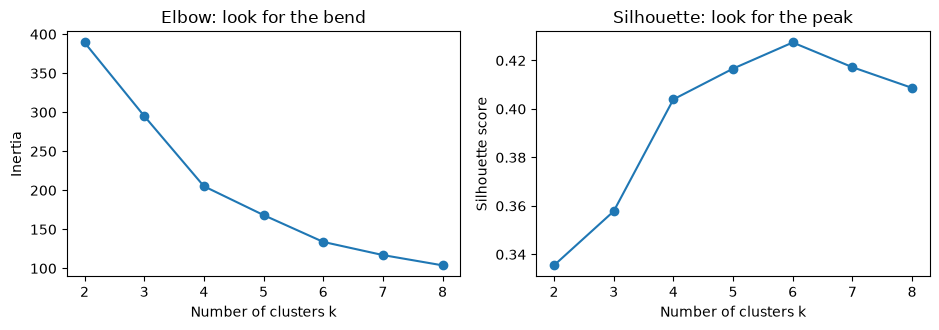
\includegraphics[width=.88\linewidth,height=5cm,keepaspectratio]{labs/visuals/04-notebook-reference.png}
\end{labvisual}
\begin{refoutput}
\begin{lstlisting}[style=utpterminal]
k=2  inertia=8600.4  silhouette=0.439
k=3  inertia=6375.8  silhouette=0.347
k=4  inertia=4963.7  silhouette=0.365
k=5  inertia=4137.7  silhouette=0.339
...
k=8  inertia=2919.8  silhouette=0.307
\end{lstlisting}
\end{refoutput}

\textbf{What it means.} The silhouette peaks at $k=2$, a split into active and inactive customers that any shopkeeper already knows. Among the richer splits, $k=4$ beats both 3 and 5. The numbers narrow the choice; what the segments are for decides it, and the next questions use four.
\end{labanswer}

\begin{labquestion}{4}{Compare K-means with DBSCAN}
K-means with four segments, against DBSCAN, which finds dense regions and leaves the rest as \emph{noise}. Here noise is not an error: it is the customers who look like no one else.
\end{labquestion}
\begin{labanswer}
\lstinputlisting[style=utppython,firstline=84,lastline=97]{all_experiments/lab04_clustering_pca/lab04_clustering_pca_worked.py}
\begin{refoutput}
\begin{lstlisting}[style=utpterminal]
K-means (k=4) silhouette: 0.365
DBSCAN clusters: 2  noise customers: 91  their share of revenue: 0.308
noise customers' median orders and spend: {'orders': 29.0, 'spend': 23419.0}
\end{lstlisting}
\end{refoutput}

\textbf{What it means.} DBSCAN finds two dense groups and refuses to place 91 customers, 1.5\% of them. Those 91 carry 30.8\% of the shop's revenue, with a median of 29 orders and \pounds 23,419: the wholesale buyers. A method allowed to say ``none of the above'' found the customers who matter most.
\end{labanswer}

\begin{labquestion}{5}{Describe the segments}
Medians describe each K-means segment in its own units, with its share of the shop's revenue.
\end{labquestion}
\begin{labanswer}
\lstinputlisting[style=utppython,firstline=99,lastline=109]{all_experiments/lab04_clustering_pca/lab04_clustering_pca_worked.py}
\begin{refoutput}
\begin{lstlisting}[style=utpterminal]
                customers  recency_days  orders   spend  revenue_share
kmeans_cluster
0                    2056         400.0     1.0   291.0          0.040
1                    1474         162.0     5.0  1587.0          0.179
2                    1117          15.0    13.0  5232.0          0.721
3                    1231          23.0     3.0   721.0          0.059
\end{lstlisting}
\end{refoutput}

\textbf{What it means.} Four segments a marketing team can act on: 2,056 lost one-time buyers who last ordered over a year ago; 1,474 lapsing regulars, worth a reminder; 1,231 recent occasional buyers, worth a second sale; and 1,117 best customers, who order every few weeks and bring in 72.1\% of all revenue. The cluster numbers are arbitrary; the names come from reading the medians.
\end{labanswer}

\begin{labquestion}{6}{Plot both clusterings}
Orders against spend, on log scales, colored by each method's labels.
\end{labquestion}
\begin{labanswer}
\lstinputlisting[style=utppython,firstline=111,lastline=124]{all_experiments/lab04_clustering_pca/lab04_clustering_pca_worked.py}

\textbf{What it means.} K-means cuts the cloud into four slices, because it always splits the space. DBSCAN draws a different line: its two dense clusters are simply the customers who ordered once and those who came back. Its noise points are the outliers, mostly at the top right, where a few customers have many orders and very large bills, plus a scattering of single unusually large orders.
\end{labanswer}

\begin{labcheckpoint}
\begin{itemize}[leftmargin=1.2em,itemsep=2pt,topsep=1pt]
  \item 779,425 clean lines from 5,878 customers.
  \item The silhouette peaks at $k=2$ (0.439); $k=4$ scores 0.365.
  \item DBSCAN leaves 91 customers as noise, and they bring 30.8\% of the revenue.
\end{itemize}
\end{labcheckpoint}

\labpartopen{Part B}{PCA on wood-defect images}{Questions 7--11 \textbullet\ Data: wood surface defects}{Compress 3,072 pixels with PCA, choose how much to keep on validation, and open the test images once.}

\begin{labquestion}{7}{Load the images}
The source holds 20,276 photos of sawn boards, collected for automated quality control, with a box around each defect. The course file holds 15,701 of those defects, cut out and shrunk to 32 by 32 colour pixels, in seven types. Most boards carry several defects, so whole boards go to one side of each split, development or test: a defect never meets its neighbour from the same board on the other side. The test images stay closed until Question~9.
\end{labquestion}
\begin{labanswer}
\lstinputlisting[style=utppython,firstline=126,lastline=150]{all_experiments/lab04_clustering_pca/lab04_clustering_pca_worked.py}
\begin{refoutput}
\begin{lstlisting}[style=utpterminal]
images: (15701, 32, 32, 3)  boards: 10358
per defect type: {'live knot': 3000, 'dead knot': 3000, 'resin': 3000, 'knot with crack': 2276,
 'crack': 2169, 'marrow': 1181, 'quartzity': 1075}
12567 development and 3134 test images; boards in both: 0
\end{lstlisting}
\end{refoutput}

\textbf{What it means.} Each image becomes a row of $32\times32\times3=3{,}072$ numbers. Neighboring pixels, and the three colours of one pixel, are strongly correlated: that redundancy is what PCA can remove. The types are not balanced, so the per-type recall in Question~9 matters as much as the accuracy.
\end{labanswer}

\textbf{Connect it to the chapter.} K-means and PCA both had no answer key, and from here on PCA is judged against one.
% Reused from chapters/14-how-unsupervised-learning-works.tex
\begin{labvisual}{Recall the chapter model}
\begin{labgraphic}
\begin{tikzpicture}[
  bx/.style={draw=UTPBlue,fill=UTPPaleBlue,rounded corners=2mm,text width=4.4cm,minimum height=1.2cm,align=center,font=\small\bfseries\color{UTPNavy}},
  arr/.style={-{Stealth[length=2.2mm]},thick,draw=UTPTeal}
]
\node[bx] (s) at (-4.3,0) {Supervised\\$X+y \longrightarrow$ predict $y$};
\node[bx] (u) at (4.3,0) {Unsupervised\\$X \longrightarrow$ discover structure};
\draw[arr] (s.east) -- node[above,font=\scriptsize\color{UTPMuted}]{remove the supplied label} (u.west);
\end{tikzpicture}
\end{labgraphic}\end{labvisual}


\begin{labquestion}{8}{Choose a PCA budget on validation}
How much variance to keep is a hyperparameter, so it is chosen on validation rows: a quarter of the development boards, split off the same way. Logistic regression on all 3,072 pixels is the reference; with that many inputs it needs up to 3,000 steps to converge.
\end{labquestion}
\begin{labanswer}
\lstinputlisting[style=utppython,firstline=152,lastline=170]{all_experiments/lab04_clustering_pca/lab04_clustering_pca_worked.py}
\begin{refoutput}
\begin{lstlisting}[style=utpterminal]
all 3,072 pixels: validation accuracy = 0.6168
90% variance:  21 components, validation accuracy = 0.5701
95% variance:  50 components, validation accuracy = 0.5919
99% variance: 248 components, validation accuracy = 0.6072
\end{lstlisting}
\end{refoutput}

\textbf{What it means.} Ninety per cent of the variance fits in just 21 directions, but those directions describe the light and colour of the wood more than the shape of a defect, and they score 0.570. The score climbs with the budget, and 99\%, 248 components, comes within a point of all 3,072 pixels. The budget is 99\%: a twelvefold compression for almost no loss.
\end{labanswer}

\begin{labquestion}{9}{Open the test images once}
The chosen budget, 99\% of the variance, is refit on all the development images and scored once on the test boards, beside logistic regression on all 3,072 pixels.
\end{labquestion}
\begin{labanswer}
\lstinputlisting[style=utppython,firstline=172,lastline=186]{all_experiments/lab04_clustering_pca/lab04_clustering_pca_worked.py}
\begin{refoutput}
\begin{lstlisting}[style=utpterminal]
FINAL TEST (3,134 images from boards never seen in development)
all 3,072 pixels accuracy: 0.6375
PCA components kept: 253  variance retained: 0.99
PCA -> logistic accuracy: 0.6331
recall per defect type: {'live knot': 0.56, 'dead knot': 0.69, 'resin': 0.73, 'knot with crack': 0.43,
 'crack': 0.72, 'marrow': 0.74, 'quartzity': 0.58}
\end{lstlisting}
\end{refoutput}

\textbf{What it means.} On boards never seen before, 253 components score 0.633 against 0.638 for every pixel: half a point for a model twelve times smaller in its inputs. Knots with cracks are the hardest type (recall 0.43), because they look like the knots they are; cracks, resin and marrow are found most often. A linear model on pixels stops near 64\%; Lab~7 asks whether a network that learns its own features can do better.
\end{labanswer}

\begin{labquestion}{10}{See what 99\% looks like}
Rebuild eight test images from 90\% and from 99\% of the variance to see what each keeps, and draw how the variance accumulates over the 3,072 directions.
\end{labquestion}
\begin{labanswer}
\lstinputlisting[style=utppython,firstline=188,lastline=220]{all_experiments/lab04_clustering_pca/lab04_clustering_pca_worked.py}
\begin{refoutput}
\begin{lstlisting}[style=utpterminal]
components for 50%, 80%, 90%, 95% and 99% of the variance: [2, 8, 21, 51, 253]
the first three components hold 0.624 of the variance
\end{lstlisting}
\end{refoutput}

\textbf{What it means.} Two directions hold half of the variance and three hold 62\%: mostly how light or dark, and how yellow, the wood is. Rebuilt from 21 components, a knot is a soft brown blur; from 253, its rings and cracks come back. Variance is not the same as usefulness: the directions that matter for telling defects apart are the faint ones, deep in the curve.
\end{labanswer}

\begin{labquestion}{11}{Save and reload the model}
Save the pipeline, reload it, and check that it still names the first test images.
\end{labquestion}
\begin{labanswer}
\lstinputlisting[style=utppython,firstline=222,lastline=229]{all_experiments/lab04_clustering_pca/lab04_clustering_pca_worked.py}
\begin{refoutput}
\begin{lstlisting}[style=utpterminal]
file size (MB): 6.26
predicted: ['knot with crack', 'knot with crack', 'dead knot', 'dead knot', 'knot with crack']
actual:    ['knot with crack', 'knot with crack', 'knot with crack', 'dead knot', 'knot with crack']
\end{lstlisting}
\end{refoutput}

\textbf{What it means.} Four of the five first test images are named correctly, and the miss is the confusion Question~9 predicted: a knot with a crack called a dead knot. The file holds the 253 components, each 3,072 numbers long, and the classifier: the price of compression is storing the directions.
\end{labanswer}

\begin{labcheckpoint}
\begin{itemize}[leftmargin=1.2em,itemsep=2pt,topsep=1pt]
  \item Keeping 99\% of the variance takes 248 components and scores 0.6072 on validation, against 0.6168 for all pixels.
  \item On the test boards: 0.6375 for all pixels and 0.6331 with 253 components.
\end{itemize}
\end{labcheckpoint}

\labpartopen{Finish}{Save the evidence, then try it yourself}{Questions 12--14}{Write the results folder, then extend the lab yourself before reading one worked solution.}

\begin{labquestion}{12}{Save the evidence}
Write the numbers above to the results folder. These files are regenerated on every run, so do not edit them by hand.
\end{labquestion}
\begin{labanswer}
\lstinputlisting[style=utppython,firstline=231,lastline=243]{all_experiments/lab04_clustering_pca/lab04_clustering_pca_worked.py}
\end{labanswer}

\labsubhead{Try it yourself}

\begin{labquestion}{13}{Try it yourself}
Cluster images without their labels. Reduce the Question~8 fitting images to 50 PCA components, run K-means with 7 clusters, one per defect type, and only then compare the clusters with the true types, with the adjusted Rand index and a table of what each cluster contains. Attempt it in this empty cell before reading the solution.
\end{labquestion}

\begin{labquestion}{14}{One solution}
The labels are used only after the clustering, to judge it. The average image of each cluster shows what K-means grouped by.
\end{labquestion}
\begin{labanswer}
\lstinputlisting[style=utppython,firstline=247,lastline=269]{all_experiments/lab04_clustering_pca/lab04_clustering_pca_worked.py}
\begin{refoutput}
\begin{lstlisting}[style=utpterminal]
adjusted Rand index against the true defect types: 0.129
         images most common type  purity
cluster
2          1570        dead knot    0.56
1          1630        live knot    0.46
3          1048            resin    0.39
...
0           380            resin    0.27
\end{lstlisting}
\end{refoutput}

\textbf{What it means.} The clusters barely match the types: an adjusted Rand index of 0.129, where 1 would be the types exactly and 0 a random split. The purest cluster is only 56\% dead knots. The average images show why: K-means grouped the defects by brightness, colour and the direction of the grain, which is what varies most in pixels, not by what a grader calls a defect. Without labels, ``similar'' means similar pixels.
\end{labanswer}

\labpartopen{After the lab}{Your turn, troubleshooting and hand-in}{Your-turn tasks \textbullet\ Expected findings \textbullet\ Troubleshooting \textbullet\ Checklists}{Extend the lab with the Your-turn tasks, compare with the expected findings, and check your work against the two checklists before you hand it in.}

\begin{yourturn}
Add new cells at the end of the notebook for these tasks, and record your numbers before reading the expected findings.
\begin{enumerate}
  \item \textbf{One start or many?} Rerun K-means on the customers at $k=4$ with \texttt{n\_init=1}, for seeds 0 to 7, and record each inertia. Then do the same for the Question~14 images at $k=7$. What does the difference say about \texttt{n\_init}?
  \item \textbf{Take the logs away.} Refit K-means at $k=4$ on the scaled but unlogged RFM columns, and compare the labels with Question~4's using \texttt{adjusted\_rand\_score}. How large are the four clusters?
  \item \textbf{Four or five?} Print the segment profile for $k=5$. Which of the four segments splits, and could a marketing team use that split?
  \item \textbf{How few components?} Score logistic regression on the Question~8 validation rows with 2, 10 and 50 components. What share of the variance do two components keep, and what are they good for?
\end{enumerate}
\end{yourturn}

\begin{expectedfindings}
\textbf{Warm-up.} Recency 8 days (from 2 December to 10 December), frequency 2, monetary value \pounds 200. On raw numbers a gap of \pounds 100,000 between two big spenders outweighs every other difference, so the few largest customers decide the clusters; logs measure spend in ratios, so \pounds 300 against \pounds 3,000 counts as much as \pounds 3,000 against \pounds 30,000.
\begin{enumerate}
  \item The customers are stable: all eight single starts end between 4,963.7 and 4,964.0. The images are not: eight starts end between 248,598 and 251,895, and only three of them land within a few units of the best. Four well-separated customer groups leave little room for a bad start, while seven overlapping defect groups in 50 dimensions leave plenty. Several starts cost little and protect against the second case.
  \item The adjusted Rand index against Question~4 is only 0.172, and the clusters hold 3,840, 1,999, 35 and 4 customers: two of the four ``segments'' are just the biggest spenders. Without the logs, the units decide the clustering.
  \item At $k=5$ the best customers split into 480 ``champions'' (median 7 days since the last order, 23 orders, \pounds 9,324) and 1,267 loyal regulars (35 days, 8 orders, \pounds 2,910). A team with a small budget for personal service may well want that split, an argument the silhouette alone cannot make.
  \item Validation accuracy is 0.420 with 2 components, 0.538 with 10 and 0.591 with 50, against 0.607 with 248. Two components keep 53.0\% of the variance, mostly the light and colour of the wood: good for drawing all the images on one page, not for telling a crack from a knot.
\end{enumerate}
\end{expectedfindings}

\begin{troubleshoot}
\begin{description}
  \item[\texttt{FileNotFoundError} for the ZIP] Keep \texttt{unsupervised/\allowbreak online\_retail\_ii/\allowbreak online\_retail\_ii.zip} zipped in \texttt{all\_datasets/}; pandas reads the CSV inside it.
  \item[A \texttt{KMeans} memory-leak warning on Windows] scikit-learn suggests setting \texttt{OMP\_NUM\_THREADS}; the results are unaffected.
  \item[Question~2 is slow] Reading a million lines takes a few seconds.
  \item[Questions~8 and~9 take a minute each] Logistic regression on 3,072 pixels needs many steps; \texttt{max\_iter=3000} lets it converge. With the default it stops early and warns.
\end{description}
\end{troubleshoot}

\begin{labchecklists}
\begin{verification}
\begin{itemize}
  \item The cleaning rules are fixed and listed, and the RFM columns are logged and scaled before clustering.
  \item The choice of $k$ is justified by the silhouette and by what the segments are for.
  \item You can say who DBSCAN's noise customers are, and why they matter.
  \item Every split keeps whole boards on one side, the PCA budget is chosen on validation rows, and the test boards are scored once.
  \item \texttt{models/wood\_pca\_logistic.joblib} reloads and names the first test images.
\end{itemize}
\end{verification}

\begin{labdeliverable}
\begin{itemize}
  \item Restart the kernel and run all cells without errors.
  \item Submit the executed notebook, including your \emph{Your turn} cells, the generated \texttt{results/lab04/} folder, and the saved model.
  \item Add a short conclusion: the segments you would give a marketing team, and why; and whether you would ship the PCA model or the raw-pixel one.
\end{itemize}
\end{labdeliverable}
\end{labchecklists}


\chapter{Anomaly Detection}
\label{ch:anomaly}

\chapterguide%
  {\chapref{ch:unsupervised}, distributions and quantiles from \chapref{ch:foundations}, plus clustering and density ideas from \chapref{ch:clustering}.}
  {score anomalies with statistical rules and see how they fail; compare distance, local density and isolation; turn a score into a review list; and evaluate alerts at a real budget.}

A security guard on a quiet night watches for whatever does not fit. Nobody gave the guard a catalog of every possible burglar. The guard knows what normal looks like, and notices departures. \term{Anomaly detection} works the same way: it ranks departures from a reference pattern, such as fraud, sensor failures or data-entry errors. Examples of the thing you are looking for are rare, expensive to label, and tomorrow's may look nothing like yesterday's.

\section{Two setups, one name}

Two closely related setups share the name:

\begin{utptable}
\begin{tabularx}{\linewidth}{@{}>{\bfseries\leavevmode\color{UTPNavy}}m{0.22\linewidth}m{0.36\linewidth}X@{}}
\toprule
\rowcolor{UTPPaleBlue!92}
\utpth{Setup} & \utpth{Training data} & \utpth{Goal} \\
\midrule
Outlier detection & The training data itself is contaminated with anomalies. & Find the anomalous observations already present in the data. \\
Novelty detection & The training data contains clean ``normal'' behavior. & Flag future observations that deviate from the learned normal pattern. \\
\bottomrule
\end{tabularx}
\end{utptable}

Because anomalies are rare and costly to label, many methods learn a reference pattern and score departures from it.

\section{Statistical rules: z-scores and IQR fences}

For a single roughly bell-shaped feature, the \term{z-score} measures how many standard deviations an observation sits from the mean:
\[
  z=\frac{x-\bar{x}}{s},
\]
with $|z|>3$ a customary alarm threshold, because under a normal distribution only about $0.3\%$ of values land that far out.

\begin{workedexample}
A temperature sensor averages $\bar{x}=50$ with standard deviation $s=5$. A reading of $68$ has $z=(68-50)/5=3.6$: flagged. A reading of $57$ has $z=1.4$: unremarkable.
\end{workedexample}

There is a trap in this rule: an outlier can hide itself, because it inflates the very mean and standard deviation that are supposed to expose it.

\begin{workedexample}
A sensor reads $10,\ 11,\ 9,\ 10,\ 12,\ 11,\ 10,\ 60$. The 60 is obviously wrong. Yet the mean is 16.62 and the standard deviation 17.55, so its z-score is only $(60-16.62)/17.55=2.47$, which does not raise the alarm. The outlier has \emph{masked} itself.

Robust statistics resist this. The median is 10.5, and the median absolute deviation (MAD) is 0.5, so the robust z-score of 60 is $0.6745\times(60-10.5)/0.5=66.8$. The IQR fences agree: with $Q_1=10$ and $Q_3=11.25$, the fences are 8.125 and 13.125, and 60 lies far outside them.
\end{workedexample}

\term{IQR fences} use quartiles (\chapref{ch:statistics}):
\[
  [\,Q_1-1.5\operatorname{IQR},\ Q_3+1.5\operatorname{IQR}\,].
\]
For $Q_1=20$ and $Q_3=30$ minutes, the fences are 5 and 45, so a 60-minute delivery is flagged without assuming normality.

Per-feature checks can miss unusual combinations of individually plausible values. Multivariate methods capture these relationships.

\section{Distance and local density}

Distance to the $k$-th nearest neighbor measures isolation, but naturally sparse groups can look anomalous. \term{Local outlier factor (LOF)} instead compares a point's density with that of its neighbors: near 1 is locally typical, and much larger values indicate local isolation.

\begin{workedexample}
A tight group has points 0.1 apart, a loose group has points 1 apart, and one stranger sits 1.0 away from the tight group.

\medskip
\centering\small
\begin{tabular}{@{}lcc@{}}
\toprule
\rowcolor{UTPPaleBlue!92}
\utpth{Point} & \utpth{Distance to third neighbor} & \utpth{Local outlier factor} \\
\midrule
Member of the tight group & 0.20 & 1.00 \\
Member of the loose group & 2.00 & 1.00 \\
The stranger & 1.20 & 4.71 \\
\bottomrule
\end{tabular}
\par\raggedright
\medskip
By plain distance, an ordinary loose-group member looks more anomalous than the stranger. LOF asks ``unusual compared with whom?'' and flags only the stranger.
\end{workedexample}

\section{Model-based scores}

Fit a Gaussian or mixture to reference data and flag low-likelihood cases (\chapref{ch:clustering}). A \term{one-class SVM} instead learns a boundary around the reference population.

\section{Isolation forests}
\label{sec:isolation-forest}

\begin{analogy}
Play a game of Guess Who with a crowd. To pick out someone with very unusual features takes one or two questions. To pick out one average person from among many similar ones takes a long time. An \term{isolation forest} plays this with random questions: it builds trees of random feature thresholds, and it scores each row by how quickly it becomes isolated.
\end{analogy}

\begin{workedexample}
Take 99 ordinary values drawn from a bell curve and one stranger at 8. Cut the range at a random point, keep the side the target is on, and repeat until the target is alone. On average the stranger takes 1.6 cuts and an ordinary value takes 9.6.
\end{workedexample}

Isolation forests need no distance metric. \term{Contamination} sets a threshold, not the true anomaly rate; Lab~5 ranks raw scores instead.

\section{Evaluating and using anomaly detectors}

Never trust the headline number alone. Lab~5's isolation forest ranks 85,443 held-out card transactions, of which 148 are fraud (0.17\%). It never sees the fraud column while fitting. Its ROC AUC is 0.95, which sounds superb. Its average precision is 0.22, which is 126 times the base rate and still modest. What a review team cares about is the list.

\begin{utptable}
\centering
\begin{tabular}{@{}cccc@{}}
\toprule
\rowcolor{UTPPaleBlue!92}
\utpth{Cases reviewed} & \utpth{Frauds found} & \utpth{Precision} & \utpth{Recall} \\
\midrule
10 & 7 & 0.700 & 0.047 \\
50 & 25 & 0.500 & 0.169 \\
100 & 39 & 0.390 & 0.264 \\
200 & 50 & 0.250 & 0.338 \\
300 & 63 & 0.210 & 0.426 \\
500 & 69 & 0.138 & 0.466 \\
1000 & 99 & 0.099 & 0.669 \\
\bottomrule
\end{tabular}
\end{utptable}

\begin{utpfig}[Precision falls as the budget grows]{Lab~5's isolation forest on 85,443 held-out transactions. Reviewing more cases finds more fraud at a falling hit rate. The base rate of 0.17\% is what reviewing at random would achieve.}{fig:precision-at-k}
\begin{tikzpicture}
\begin{axis}[logaxis, width=0.72\linewidth, height=4.8cm, xlabel={cases reviewed}, ylabel={share}, xmin=0, xmax=1050, ymin=0, ymax=1.05,
  legend style={at={(0.97,0.55)},anchor=east}]
\addplot[draw=UTPBlue,mark=*,mark size=1.4pt,thick] coordinates {(10,0.7)(50,0.5)(100,0.39)(200,0.25)(300,0.21)(500,0.138)(1000,0.099)};
\addlegendentry{precision: fraud rate in the list}
\addplot[draw=UTPOrange,mark=square*,mark size=1.4pt,thick] coordinates {(10,0.047)(50,0.169)(100,0.264)(200,0.338)(300,0.426)(500,0.466)(1000,0.669)};
\addlegendentry{recall: share of all fraud found}
\addplot[draw=UTPMuted,dashed,domain=0:1050] {0.0017};
\addlegendentry{base rate, 0.17\%}
\end{axis}
\end{tikzpicture}
\end{utpfig}

\begin{itemize}
  \item For distance- and kernel-based detectors, apply the scaling rule from \secref{sec:scaling}.
  \item Choose thresholds from consequences --- how many alarms per day can be investigated? --- not from statistical custom.
  \item Anomalies may be errors or important rare events. Investigate before deleting.
\end{itemize}

\section{The shape of an anomaly problem}

Anomaly detection differs from classification in one important way: you usually cannot see many examples of the thing you are looking for.

\begin{utpfig}[Two views of an anomaly problem]{Two views of an anomaly problem. Distance and density place anomalies outside the normal region; a score and a threshold you choose turn that into a list of flagged cases.}{fig:anomaly-views}
\begin{tikzpicture}[font=\scriptsize]
\begin{scope}
\draw[draw=UTPMuted,fill=white] (0,0) rectangle (4.2,2.9);
\foreach \p in {(1.5,1.4),(1.8,1.6),(1.6,1.1),(2.0,1.3),(1.3,1.7),(2.2,1.6),(1.9,0.9),
                (1.4,1.25),(2.1,1.1),(1.7,1.45),(2.3,1.35),(1.55,0.85),(2.05,1.65)}
  \fill[UTPBlue] \p circle (2.4pt);
\draw[UTPTeal,thick,dashed] (1.8,1.32) circle (0.95);
\fill[UTPRed] (3.5,2.4) circle (2.8pt);
\fill[UTPRed] (0.5,0.4) circle (2.8pt);
\node[color=UTPRed,anchor=east] at (4.15,2.72) {anomalies};
\node[color=UTPTeal] at (1.8,-0.35) {the "normal" region};
\node[font=\small\bfseries\color{UTPNavy}] at (2.1,3.25) {Distance / density view};
\end{scope}
\begin{scope}[xshift=5.6cm]
\draw[draw=UTPMuted,fill=white] (0,0) rectangle (4.6,2.9);
\draw[-{Stealth[length=2mm]},UTPMuted] (0.3,0.45) -- (4.35,0.45);
\node[color=UTPMuted,anchor=north,inner sep=1pt] at (2.3,0.40) {anomaly score};
\draw[UTPBlue,very thick] plot[smooth,domain=0.4:4.3,samples=60]
  (\x, {0.45+2.0*exp(-((\x-1.3)^2)/0.28)});
\draw[UTPRed,very thick,dashed] (2.85,0.45) -- (2.85,2.6);
\node[color=UTPRed,anchor=west,align=left] at (2.95,2.2) {threshold\\you choose};
\node[color=UTPGreen] at (1.3,2.68) {normal};
\node[color=UTPRed,anchor=west] at (3.1,0.85) {flagged};
\node[font=\small\bfseries\color{UTPNavy}] at (2.3,3.25) {Score-and-threshold view};
\end{scope}
\end{tikzpicture}
\end{utpfig}

\begin{keyidea}
Choose thresholds or review batches for actual capacity and error costs; a high score is not a verdict.
\end{keyidea}

\section{From anomaly score to investigation}

Define the review process alongside the scoring model.

\begin{utptable}
\begin{tabularx}{\linewidth}{@{}>{\bfseries\leavevmode\color{UTPNavy}}m{0.35\linewidth}X@{}}
\toprule
\rowcolor{UTPPaleBlue!92}
\utpth{Question} & \utpth{Practical consequence} \\
\midrule
How many cases can be reviewed? & Choose a top-$k$ or score threshold that respects review capacity. \\
What happens after a flag? & Define whether the case is blocked, queued, inspected, or merely logged. \\
Which false alert is costly? & Track precision among reviewed cases and the burden on users or analysts. \\
Can normal behavior change? & Monitor score distributions and retrain or recalibrate when the reference population drifts. \\
Can labels arrive later? & Use confirmed outcomes to evaluate ranking quality and eventually consider a supervised model. \\
\bottomrule
\end{tabularx}
\end{utptable}

\recipecard{Isolation forest}{Many trees of random splits. A row's score comes from how shallow its leaf is on average.}{None in the usual sense: the method has no target and no loss to reduce.}{None. Trees are grown at random, and the only choices are their number and the sample size.}

\begin{modelcard}{Anomaly Detection - Quick Guide}
\begin{tabularx}{\linewidth}{@{}>{\bfseries\leavevmode\color{UTPNavy}}p{0.25\linewidth}X@{}}
Anomaly detection asks & Which observations are unusually inconsistent with a reference pattern? \\
Useful methods & Robust statistical rules, distance/local-density methods, isolation forest, and one-class models. \\
Output & An anomaly score or ranking; a later policy converts that score into an alert. \\
Evaluation & Precision among reviewed cases, PR AUC when labels exist, stability, and downstream review value. \\
Main risks & Rare does not always mean harmful; distribution shift can make yesterday's normality model obsolete. \\
\end{tabularx}
\end{modelcard}

\begin{chapterrecap}
\begin{itemize}
  \item An anomaly score ranks departures from a reference pattern. It is not a probability of fraud.
  \item The z-score can be masked by the outlier itself, so prefer the median, the MAD and the IQR.
  \item Distance alone penalizes naturally sparse groups; LOF judges a point against its own neighborhood.
  \item Isolation forests need no distance: strangers separate after a few random cuts.
  \item Evaluate at the real review budget. A ROC AUC of 0.95 and a 39\% hit rate in the top 100 describe the same ranking.
\end{itemize}
\end{chapterrecap}

\begin{quickcheck}
\begin{enumerate}
  \item Why is an anomaly score not automatically a probability of fraud, failure or error?
  \item How does a fixed review capacity turn anomaly detection into a ranking problem?
  \item What is the difference between detecting outliers in the training sample and novelty detection for future observations?
  \item Readings are $5,5,6,4,5,50$. Compute the median and MAD. Is the 50 flagged by a robust z-score above 3?
  \item In the fraud table above, why does recall keep rising when precision falls?
\end{enumerate}
\end{quickcheck}

\begin{checkanswers}
\begin{enumerate}
  \item It measures how unusual a row is under a reference pattern. Unusual can be harmless, and harmful can look ordinary, and nothing calibrates the score to outcomes.
  \item If the team can check only 100 cases, the only question is which 100, so the quality of the top of the ranking is what counts.
  \item Outlier detection looks for anomalies already in a contaminated training set. Novelty detection learns from clean normal data and flags new rows that differ from it.
  \item Median 5, and the absolute deviations are $0,0,1,1,0,45$, so the MAD is 0.5. The robust z-score is $0.6745\times45/0.5\approx60.7$, so yes.
  \item Recall counts frauds found out of all 45, so each new find raises it. Precision divides by the size of the list, which grows faster than the finds.
\end{enumerate}
\end{checkanswers}


\part{Advanced Concepts}
\chapter{Semi-Supervised and Active Learning}
\label{ch:semi-supervised}

\chapterguide%
  {Supervised learning, validation, classification probabilities, and similarity measures. Lab~5 follows this chapter and also uses \chapref{ch:anomaly}.}
  {say when unlabeled data can help; trace self-training and label propagation by hand; explain how pseudo-labels can reinforce mistakes; choose what to label by uncertainty; and judge any such method against a labeled-only baseline on genuine labels.}

Back to the map question: does your log hold the answers? So far the answer was yes or no. Often it is ``some of them.'' Photos, scans and messages are cheap to collect, and a person's time to label them is not.

\begin{analogy}
A student has a thick workbook and an answer key for only a few pages. One strategy is to mark the rest yourself, using only the answers you feel very sure about, and study from those too. That is \term{semi-supervised learning}, and it works if your confidence is earned. Another strategy is to take the questions you are least sure of to the teacher, who has time for only a few. That is \term{active learning}.
\end{analogy}

\section{The data setting}

Let
\[
  \mathcal{D}_L=\{(\bm{x}_i,y_i)\}_{i=1}^{n_L}
\]
be the labeled data and
\[
  \mathcal{D}_U=\{\bm{x}_j\}_{j=1}^{n_U}
\]
be the unlabeled data, usually with $n_U\gg n_L$.

Unlabeled data reveal concentration and similarity, not class meaning.

\section{When unlabeled data can help}

Semi-supervised methods rely on assumptions such as:

\begin{itemize}
  \item nearby observations are likely to share a label;
  \item observations in the same dense region are likely to share a label;
  \item the decision boundary should pass through low-density areas rather than cutting through a cluster.
\end{itemize}

Nearby observations or shared clusters need not share labels. Unlabeled structure helps only when it relates to the target.

\section{Self-training and pseudo-labeling}

Self-training is the simplest semi-supervised approach.

\begin{utpsteps}
  \item Train a supervised model on the labeled data.
  \item Predict labels and probabilities for the unlabeled data.
  \item Keep only predictions with confidence above a strict threshold.
  \item Add those pseudo-labeled examples to the training set, usually with lower weight.
  \item Retrain the model and repeat for a limited number of rounds.
\end{utpsteps}

\begin{workedexample}
One column, labels for $x=1,2$ (class 0) and $x=8,9$ (class 1), and six unlabeled rows. Adopt a pseudo-label only when the model's chance is at least 0.8 or at most 0.2.

\medskip
\centering\small
\begin{tabular}{@{}cll@{}}
\toprule
\rowcolor{UTPPaleBlue!92}
\utpth{Round} & \utpth{Chance of class 1 for the unlabeled rows} & \utpth{Adopted} \\
\midrule
1 & $x=3$: 0.17,\ 4: 0.31,\ 5: 0.50,\ 6: 0.69,\ 7: 0.83,\ 10: 0.98 & 3, 7, 10 \\
2 & $x=4$: 0.28,\ 5: 0.51,\ 6: 0.73 & none, so stop \\
\bottomrule
\end{tabular}
\par\raggedright
\medskip
The clear rows join the training set, and the ambiguous rows 4, 5 and 6 stay unlabeled. Tighten the threshold and fewer rows join; loosen it and the model's mistakes start to count as facts.
\end{workedexample}

\begin{pitfall}
Pseudo-labeling can reinforce confident mistakes. Limit rounds, check class balance, and validate against human labels.
\end{pitfall}

\begin{workedexample}
Does it help? In Lab~5 a pool holds 8,003 messages to a bank's support chat in 77 intents, and only 1,000 keep their labels. A plain model on those scores 0.638 on validation; self-training adopts 486 pseudo-labels, 98.8\% of them right, and scores 0.632, against 0.882 with every label: no gain, because the model is sure only about messages it already gets right. Lower the confidence threshold to 0.5, and it adopts 3,604 pseudo-labels, only 76.8\% of them right, and falls to 0.596: every wrong label is learned as if it were true. Always compute the baseline.
\end{workedexample}

\section{Graph-based label propagation}

Connect similar observations with weighted edges, and let labels spread through the graph like news through a group of friends. Each unlabeled node repeatedly takes the average of its neighbors, while labeled nodes stay fixed.

\begin{workedexample}
A chain of six nodes, with the left end labeled 1 and the right end labeled 0. The unlabeled nodes start at 0.5 and are updated left to right, using the newest values. After one sweep they read $0.75,\ 0.5,\ 0.5,\ 0.25$. After two: $0.75,\ 0.625,\ 0.375,\ 0.25$. They settle at $0.8,\ 0.6,\ 0.4,\ 0.2$, a smooth slope between the two labels, because each value is the mean of its two neighbors.
\end{workedexample}

\begin{utpfig}[Graph-based label propagation]{Graph-based label propagation. Similar observations are joined by edges, and the two known labels spread through their own connected groups to the unlabeled points.}{fig:label-propagation}
\begin{tikzpicture}[
  node/.style={circle,draw=UTPMuted,minimum size=6mm,inner sep=0pt},
  labA/.style={node,fill=UTPBlue!35,draw=UTPBlue},
  labB/.style={node,fill=UTPOrange!35,draw=UTPOrange},
  unlab/.style={node,fill=white},
  edge/.style={draw=UTPMuted!60,thick}
]
\node[labA] (a1) at (0,1.2) {A};
\node[unlab] (a2) at (1.1,1.7) {};
\node[unlab] (a3) at (1.5,0.7) {};
\node[unlab] (a4) at (2.5,1.4) {};
\node[labB] (b1) at (5.2,1.2) {B};
\node[unlab] (b2) at (4.1,1.7) {};
\node[unlab] (b3) at (3.8,0.65) {};
\node[unlab] (b4) at (5.7,0.25) {};
\draw[edge] (a1)--(a2)--(a4)--(a3)--(a1);
\draw[edge] (a2)--(a3);
\draw[edge] (b1)--(b2)--(b3)--(b1);
\draw[edge] (b1)--(b4)--(b3);
\draw[dashed,UTPMuted!45] (a4)--(b3);
\end{tikzpicture}
\end{utpfig}

This works well when similarity is meaningful and clusters line up with classes. It can fail when the graph connects unlike observations or when feature scaling is poor.

\section{Co-training}

Co-training fits two views, such as webpage text and links, whose models exchange high-confidence pseudo-labels.

Both views must be informative and offer complementary errors; nearly identical views add little.

\section{Active learning}

Active learning asks which labels would be most informative, within a fixed budget.

Common selection strategies include:

\begin{utptable}
\begin{tabularx}{\linewidth}{@{}>{\bfseries\leavevmode\color{UTPNavy}}m{0.26\linewidth}X@{}}
\toprule
\rowcolor{UTPPaleBlue!92}
\utpth{Selection strategy} & \utpth{Which examples it chooses} \\
\midrule
Uncertainty sampling & Examples whose predicted probabilities are closest to a tie. \\
Query by disagreement & Examples on which several models disagree. \\
Diversity sampling & Uncertain examples that also cover different regions of the feature space. \\
Expected impact & Examples whose labels are estimated to improve the model most or reduce decision cost. \\
\bottomrule
\end{tabularx}
\end{utptable}

\begin{workedexample}
A model gives these unlabeled rows a chance of class 1: $0.97,\ 0.52,\ 0.10,\ 0.61,\ 0.48,\ 0.88$. With budget for two labels, uncertainty sampling asks about the 0.52 and the 0.48, which are nearest to a coin flip. A label on the 0.97 row would probably just confirm what the model already believes.
\end{workedexample}

\begin{utpfig}[The active-learning loop]{The active-learning loop. The model selects useful unlabeled cases, a human labels them, and the labeled set grows before the model is trained again.}{fig:active-loop}
\begin{tikzpicture}[
  node distance=0.55cm,
  box/.style={draw=UTPBlue,fill=UTPPaleBlue,rounded corners=2mm,minimum width=2.35cm,minimum height=0.82cm,align=center,font=\small\color{UTPNavy}},
  arr/.style={-{Stealth[length=2mm]},thick,draw=UTPTeal}
]
\node[box] (train) {Train model};
\node[box,right=of train] (select) {Select useful\\unlabeled cases};
\node[box,right=of select] (label) {Human labels\\the cases};
\node[box,right=of label] (add) {Add to labeled\\training set};
\draw[arr] (train)--(select);\draw[arr] (select)--(label);\draw[arr] (label)--(add);
\draw[arr] (add.south) to[bend left=28] (train.south);
\end{tikzpicture}
\end{utpfig}

\begin{utpfig}[Uncertainty sampling, step by step]{Uncertainty sampling, step by step: train on the labels you have, score every unlabeled example, select the most uncertain ones, ask a human to label them, and repeat until the labeling budget runs out.}{fig:uncertainty-sampling}
\begin{tikzpicture}[
  node distance=1.05cm and 1.35cm,
  st/.style={draw=UTPBlue,fill=UTPPaleBlue,rounded corners=2mm,minimum width=5.25cm,minimum height=1.0cm,inner xsep=3pt,align=center,font=\scriptsize\bfseries\color{UTPNavy}},
  hum/.style={draw=UTPOrange,fill=UTPPaleOrange,rounded corners=2mm,minimum width=5.25cm,minimum height=1.0cm,inner xsep=3pt,align=center,font=\scriptsize\bfseries\color{UTPNavy}},
  arr/.style={-{Stealth[length=2.2mm]},thick,draw=UTPTeal}
]
\node[st] (train) {1. Train using the labels you have};
\node[st,right=of train] (score) {2. Score every unlabeled example};
\node[st,below=of score] (pick) {3. Select the most uncertain examples};
\node[hum,below=of train] (ask) {4. Ask a human to label those examples};
\draw[arr] (train) -- (score);
\draw[arr] (score) -- (pick);
\draw[arr] (pick) -- (ask);
\draw[arr] (ask) -- (train);
\node[font=\scriptsize\itshape\color{UTPMuted},align=center] at ($(train)!0.5!(pick)$) {repeat until the budget runs out};
\end{tikzpicture}
\end{utpfig}

\begin{utpfig}[Uncertainty against random querying]{Lab~5's support-message simulation: validation accuracy on 2,000 messages against labels bought, from 154 labels (2 per intent), buying 100 per round. The two policies are level for two rounds; from then on uncertainty sampling leads.}{fig:active-curve}
\begin{tikzpicture}
\begin{axis}[logaxis, width=0.72\linewidth, height=4.8cm, xlabel={labels bought}, ylabel={validation accuracy}, xmin=100, xmax=1100, ymin=0.28, ymax=0.75,
  yticklabel style={/pgf/number format/fixed,/pgf/number format/precision=2}, legend style={at={(0.97,0.05)},anchor=south east}]
\addplot[draw=UTPBlue,mark=*,mark size=1.4pt,thick] coordinates {(154,0.319)(254,0.36)(354,0.464)(454,0.532)(554,0.594)(654,0.616)(754,0.653)(854,0.674)(954,0.7)(1054,0.712)};
\addlegendentry{uncertainty sampling}
\addplot[draw=UTPOrange,mark=square*,mark size=1.4pt,thick] coordinates {(154,0.319)(254,0.368)(354,0.438)(454,0.505)(554,0.546)(654,0.579)(754,0.606)(854,0.631)(954,0.648)(1054,0.679)};
\addlegendentry{random querying}
\end{axis}
\end{tikzpicture}
\end{utpfig}

On the official test messages the lead holds, 0.725 against 0.682 with 1,054 labels each. Seventy-seven intents with many near neighbors make many hard boundaries, which is when active learning earns its keep. A model that knows too little cannot tell which questions are informative, so start from a sample of every class before letting uncertainty choose.

\section{A safe practical workflow}

\begin{utpsteps}
  \item Create fixed, human-labeled validation and test sets before using unlabeled data.
  \item Train a supervised baseline using only the labeled training set.
  \item Inspect whether similarity or cluster structure appears connected to the label.
  \item Add one semi-supervised or active-learning method at a time.
  \item Compare against the labeled-only baseline using the same evaluation protocol.
  \item Review performance by class and subgroup, not only overall average performance.
  \item Keep a record of which labels came from humans and which came from the model.
\end{utpsteps}

\recipecard{Self-training}{Any supervised model that outputs probabilities.}{That model's usual loss, computed on real labels and adopted pseudo-labels.}{Fit, adopt the confident predictions, refit, repeat until nothing new is adopted.}

\begin{modelcard}{Semi-Supervised and Active Learning - Quick Guide}
\begin{tabularx}{\linewidth}{@{}>{\bfseries\leavevmode\color{UTPNavy}}p{0.24\linewidth}X@{}}
Best when & Human labels are expensive, unlabeled examples are plentiful, and feature-space structure relates to the label. \cr
Start with & A supervised baseline and a fixed human-labeled validation/test set. \cr
Main controls & Confidence threshold, number of pseudo-labeling rounds, graph similarity, labeling budget, query strategy. \cr
Main risks & Confirmation bias, class imbalance, poor similarity measures, sampling only unusual cases, changing labeling standards. \cr
\end{tabularx}
\end{modelcard}

\begin{keyidea}
Unlabeled data provides structure, not truth. Human labels remain the source of meaning and the basis of fair evaluation.
\end{keyidea}

\begin{chapterrecap}
\begin{itemize}
  \item Unlabeled rows reveal where data lies, not what it means. They help only if that structure lines up with the label.
  \item Self-training adopts confident predictions as labels, and label propagation spreads known labels over a similarity graph. Both can turn mistakes into facts.
  \item Active learning spends a labeling budget where the model is least sure.
  \item Keep human-labeled validation and test sets, and compare with a labeled-only baseline. In Lab~5 the baseline showed that self-training gained nothing, and that trusting it more made it worse.
\end{itemize}
\end{chapterrecap}

\begin{quickcheck}
\begin{enumerate}
  \item Why can pseudo-labeling reinforce mistakes even when the model is highly confident?
  \item What does an active-learning query strategy try to spend the labeling budget on?
  \item Why must final validation and test labels come from a genuine labeling source rather than from the model itself?
  \item Chain nodes hold $1,\ ?,\ ?,\ 0$. At rest, what are the two unknown values?
  \item Self-training scored 0.632 and labels-only 0.638 in Lab~5. Which do you ship, and what would you try before giving up on the unlabeled messages?
\end{enumerate}
\end{quickcheck}

\begin{checkanswers}
\begin{enumerate}
  \item Confidence is not correctness. A wrong pseudo-label joins the training set as if true, the refitted model becomes more confident in the same direction, and the error compounds.
  \item The rows whose labels are expected to help most, such as those closest to a coin flip, or those several models disagree on.
  \item A model cannot grade itself. Scores against its own output would measure self-agreement rather than accuracy.
  \item Each equals the mean of its neighbors, so $2/3$ and $1/3$.
  \item The labels-only model: self-training is slower and no better, and 0.6 points is about 12 of 2,000 validation messages. Before giving up on the unlabeled pool, try active learning, which gained about four points in Lab~5.
\end{enumerate}
\end{checkanswers}

\labsection{5}{Unsupervised learning II: anomaly detection and limited labels}{sec:lab05-anomaly-labels}

\begin{labproject}{Learn when labels are absent, rare, or expensive}
\textbf{Read first.} Chapter~\ref{ch:anomaly} for Part~A and Chapter~\ref{ch:semi-supervised} for Part~B.\\
\textbf{Goal.} Score an anomaly ranking with labels the model never saw, judge it at a real review budget, then simulate two ways of coping with few labels: self-training and active learning.\\
\textbf{Scenario.} A card company can review only so many transactions a day. A hospital has plenty of scans and little expert time. Both have the same problem from opposite ends: labels are the expensive part.\\
\textbf{Data.} \texttt{all\_datasets/credit\_card\_fraud\_dataset.csv} and \texttt{breast\_cancer\_dataset.csv}.\\
\textbf{Notebook.} \texttt{all\_experiments/lab05\_anomaly\_limited\_labels\_worked.ipynb}.\\
\textbf{Hand in.} The executed notebook, \texttt{results/lab05/} and a short conclusion, as listed in the checklist at the end of this sheet.
\end{labproject}

\begin{labmode}
\begin{enumerate}
  \item Activate your course environment and confirm that both data files are in \texttt{all\_datasets/}.
  \item Check the small worked numbers of Chapters~\ref{ch:anomaly} and~\ref{ch:semi-supervised}. The last line must read \texttt{Every number above matches the book.}
  \item Start Jupyter from \texttt{all\_experiments/}, open the notebook, and choose \textbf{Restart Kernel and Run All Cells}. It takes a few seconds.
\end{enumerate}
\begin{lstlisting}[style=utpterminal]
python all_experiments/demo_unsupervised.py
cd all_experiments
jupyter lab
\end{lstlisting}
Prefer a plain script? From the course folder, \texttt{python all\_experiments/lab05\_anomaly\_limited\_labels\_worked.py} runs the same code and writes the same evidence.
\end{labmode}

\courselabflow{Hide labels}{Rank anomalies}{Acquire labels}{Compare baseline}


\labroutine

\begin{yourturn}
\textbf{Warm-up on paper.} Do these before opening the notebook.
\begin{enumerate}
  \item An analyst reviews the top 10 cases of a ranking, and their true labels are $0,0,1,0,1,0,0,1,0,0$. There are 45 frauds among 3,000 cases. What are precision at 10 and recall at 10, and how many times better than random is that? (0.30; 3/45 = 0.067; 0.30/0.015 = 20 times.)
  \item A self-training model is 95\% sure of an unlabeled row, and it is wrong. What happens to that row on the next round, and to the rows near it? (It joins the training set as if true, so the model grows more confident around it, and nearby rows follow.)
\end{enumerate}
\end{yourturn}

\begin{labquestion}{1}{Setup}
Run the imports and paths first, and keep this kernel for the later questions.
\end{labquestion}
\begin{labanswer}
\lstinputlisting[style=utppython,firstline=8,lastline=26]{all_experiments/lab05_anomaly_limited_labels_worked.py}
\begin{refoutput}
\begin{lstlisting}[style=utpterminal]
course folder: MACHINE LEARNING
\end{lstlisting}
\end{refoutput}
\end{labanswer}

\labpart{Part A --- Isolation Forest fraud ranking}

\begin{labquestion}{2}{Fit an Isolation Forest without labels}
Ten thousand card transactions, of which about 1.5\% are fraud. An Isolation Forest never sees the \texttt{is\_fraud} column: it builds random trees, and scores each transaction by how quickly it can be isolated from the rest. The labels are held back and used only to judge the ranking afterwards.
\end{labquestion}
\begin{labanswer}
\courselabtrace{Spend labels where they help}{Pool}{Keep an unlabeled pool and a fixed test set}{Query}{Choose uncertain pool examples for annotation}{Update}{Refit after queries; score only the fixed test set}

\lstinputlisting[style=utppython,firstline=28,lastline=44]{all_experiments/lab05_anomaly_limited_labels_worked.py}

\textbf{What it means.} \texttt{forest.fit(X\_train)} takes no labels. Higher scores mean more unusual, which is why the code negates \texttt{decision\_function}. 7,000 rows fit the forest and 3,000 judge it.
\end{labanswer}

\begin{labquestion}{3}{Score the ranking}
Two summary numbers, then the one that matters in practice. ROC AUC judges the whole ranking. Average precision focuses on the rare positive class, and it is far more demanding when only 1.5\% of rows are positive. An analyst, though, will only ever look at the top of the list, so precision among the top 100 is the operational number.
\end{labquestion}
\begin{labanswer}
\courselabtrace{Trace the actual fraud review budget}{1. Input / state}{anomaly\_score negates decision\_function so higher means more unusual; ranked sorts descending.}{2. Operation}{review\_budget is 100; take ranked.head(review\_budget) and inspect fraud\_label.}{3. Check}{top\_k\_precision is the mean of those 100 binary labels; prevalence is the comparison baseline.}

\lstinputlisting[style=utppython,firstline=46,lastline=59]{all_experiments/lab05_anomaly_limited_labels_worked.py}
\begin{refoutput}
\begin{lstlisting}[style=utpterminal]
fraud prevalence: 0.015
ROC AUC: 0.9518
average precision: 0.2249  ( 15.0 x prevalence)
fraud found in the top 100: 20%
      fraud_label  anomaly_score  amount
6394            0       0.212892  840.89
5883            0       0.168657  978.56
1623            1       0.166446  569.02
...
\end{lstlisting}
\end{refoutput}

\textbf{What it means.} A ROC AUC of 0.95 looks excellent. Average precision of 0.22 is the more honest number, still fifteen times the base rate. Reviewing the top 100 finds 20 frauds of the 45 present. Notice that the single most unusual transaction is not fraud: unusual and fraudulent are different things.
\end{labanswer}

\begin{labquestion}{4}{Plot scores and precision at $k$}
Two pictures. On the left, the score distributions of fraud and non-fraud overlap, which is where the false alarms come from. On the right, precision as a function of how many cases are reviewed: the curve every review team should see before choosing a budget.
\end{labquestion}
\begin{labanswer}
\lstinputlisting[style=utppython,firstline=61,lastline=80]{all_experiments/lab05_anomaly_limited_labels_worked.py}
\begin{labvisual}{Reference plot from the supplied notebook}
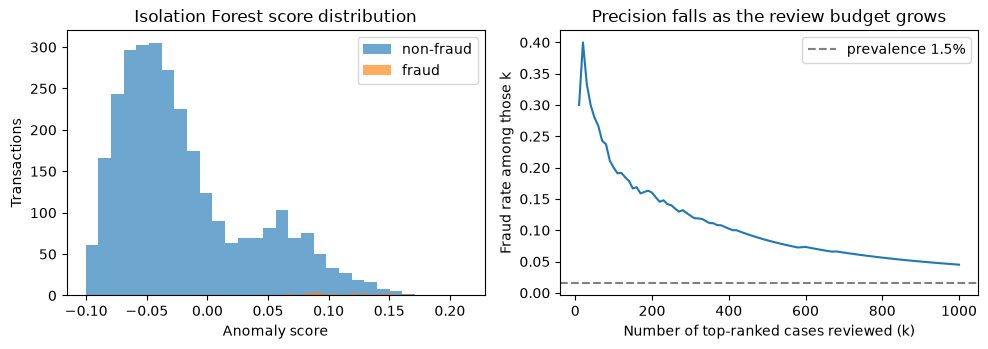
\includegraphics[width=.88\linewidth,height=5cm,keepaspectratio]{labs/visuals/05-notebook-reference.png}
\end{labvisual}

\textbf{What it means.} Fraud scores sit to the right, but non-fraud rows outnumber them about 65 to 1, so even a small overlap produces many false alarms. That is how ROC AUC can look excellent while precision is modest. The right-hand curve starts high and decays towards the base rate; a team with a fixed budget should read its expected hit rate off this curve.
\end{labanswer}

\labpart{Part B --- Self-training and active learning with few labels}

\begin{labquestion}{5}{Split the cancer data three ways}
Now the opposite problem: plenty of rows, but labels are expensive. The breast-cancer data is split three ways. The \emph{pool} is where labels can be bought, the \emph{validation} set judges each policy during development, and the \emph{test} set is sealed until both policies are finished.
\end{labquestion}
\begin{labanswer}
\lstinputlisting[style=utppython,firstline=82,lastline=102]{all_experiments/lab05_anomaly_limited_labels_worked.py}
\begin{refoutput}
\begin{lstlisting}[style=utpterminal]
pool: 319  validation: 107  test: 143
\end{lstlisting}
\end{refoutput}

\textbf{What it means.} The validation and test rows always keep their genuine labels, because the policies are judged against those.
\end{labanswer}

\begin{labquestion}{6}{Self-train from 30\% of the labels}
Self-training hides 70\% of the pool labels (scikit-learn uses $-1$ for ``unknown''), fits on the rest, then lets the model label any unlabeled row it is at least 90\% sure about, and refits. It can help when the confident predictions are right; it can also teach the model its own mistakes.
\end{labquestion}
\begin{labanswer}
\lstinputlisting[style=utppython,firstline=104,lastline=114]{all_experiments/lab05_anomaly_limited_labels_worked.py}
\begin{refoutput}
\begin{lstlisting}[style=utpterminal]
labels kept: 89 of 319
self-training validation accuracy: 0.963
\end{lstlisting}
\end{refoutput}

\textbf{What it means.} That sounds good, but is it good compared with what? Your-turn task~2 asks for the baseline this cell does not compute.
\end{labanswer}

\textbf{Connect it to the chapter.} A score is only useful with a threshold you chose, and a limited label budget is the same kind of decision.
% Reused from chapters/17-anomaly-detection.tex
\begin{labvisual}{Recall the chapter model}
\begin{labgraphic}
\begin{tikzpicture}[font=\scriptsize]
\begin{scope}
\draw[draw=UTPMuted,fill=white] (0,0) rectangle (4.2,2.9);
\foreach \p in {(1.5,1.4),(1.8,1.6),(1.6,1.1),(2.0,1.3),(1.3,1.7),(2.2,1.6),(1.9,0.9),
                (1.4,1.25),(2.1,1.1),(1.7,1.45),(2.3,1.35),(1.55,0.85),(2.05,1.65)}
  \fill[UTPBlue] \p circle (2.4pt);
\draw[UTPTeal,thick,dashed] (1.8,1.32) circle (0.95);
\fill[UTPRed] (3.5,2.4) circle (2.8pt);
\fill[UTPRed] (0.5,0.4) circle (2.8pt);
\node[color=UTPRed,anchor=east] at (4.15,2.72) {anomalies};
\node[color=UTPTeal] at (1.8,-0.35) {the "normal" region};
\node[font=\small\bfseries\color{UTPNavy}] at (2.1,3.25) {Distance / density view};
\end{scope}
\begin{scope}[xshift=5.6cm]
\draw[draw=UTPMuted,fill=white] (0,0) rectangle (4.6,2.9);
\draw[-{Stealth[length=2mm]},UTPMuted] (0.3,0.45) -- (4.35,0.45);
\node[color=UTPMuted,anchor=north,inner sep=1pt] at (2.3,0.40) {anomaly score};
\draw[UTPBlue,very thick] plot[smooth,domain=0.4:4.3,samples=60]
  (\x, {0.45+2.0*exp(-((\x-1.3)^2)/0.28)});
\draw[UTPRed,very thick,dashed] (2.85,0.45) -- (2.85,2.6);
\node[color=UTPRed,anchor=west,align=left] at (2.95,2.2) {threshold\\you choose};
\node[color=UTPGreen] at (1.3,2.68) {normal};
\node[color=UTPRed,anchor=west] at (3.1,0.85) {flagged};
\node[font=\small\bfseries\color{UTPNavy}] at (2.3,3.25) {Score-and-threshold view};
\end{scope}
\end{tikzpicture}
\end{labgraphic}\end{labvisual}


\begin{labquestion}{7}{Simulate active learning}
Active learning chooses \emph{which} labels to buy. Both policies start from the same 40 labels and buy 15 more per round. Uncertainty sampling asks for the rows whose predicted probability is closest to 0.5, where the model is least sure. Random querying is the control: same budget, no strategy.
\end{labquestion}
\begin{labanswer}
\lstinputlisting[style=utppython,firstline=116,lastline=145]{all_experiments/lab05_anomaly_limited_labels_worked.py}
\begin{refoutput}
\begin{lstlisting}[style=utpterminal]
round 1: labels= 40  uncertainty=0.944  random=0.944
round 2: labels= 55  uncertainty=0.925  random=0.953
round 3: labels= 70  uncertainty=0.981  random=0.963
round 4: labels= 85  uncertainty=0.953  random=0.963
round 5: labels=100  uncertainty=0.953  random=0.953
round 6: labels=115  uncertainty=0.953  random=0.953
round 7: labels=130  uncertainty=0.953  random=0.963
round 8: labels=145  uncertainty=0.953  random=0.963
\end{lstlisting}
\end{refoutput}

\textbf{What it means.} No line differs by more than three rows out of 107 (one row is 0.009), so this is mostly noise. Neither policy pulls clearly ahead.
\end{labanswer}

\begin{labquestion}{8}{Plot label efficiency}
Put both curves on one chart, so that the whole run can be read at a glance.
\end{labquestion}
\begin{labanswer}
\lstinputlisting[style=utppython,firstline=147,lastline=156]{all_experiments/lab05_anomaly_limited_labels_worked.py}

\textbf{What it means.} Both curves start at the same point and flatten within a few rounds. This table is simply easy: 40 labels already give a good linear model, so no policy has much left to gain. Active learning earns its keep where the boundary is genuinely uncertain.
\end{labanswer}

\begin{labquestion}{9}{Open the test set once for each policy}
Both policies are finished, so the test set is opened once for each.
\end{labquestion}
\begin{labanswer}
\lstinputlisting[style=utppython,firstline=158,lastline=164]{all_experiments/lab05_anomaly_limited_labels_worked.py}
\begin{refoutput}
\begin{lstlisting}[style=utpterminal]
final test accuracy, uncertainty sampling: 0.972
final test accuracy, random querying:     0.972
\end{lstlisting}
\end{refoutput}

\textbf{What it means.} A tie. Uncertainty sampling did not win, because this dataset is too easy for the policy to matter. The Try-it starts from fewer labels to look for the regime where it does help.
\end{labanswer}

\labpart{Evidence}

\begin{labquestion}{10}{Save the evidence}
Write the numbers above to the results folder. These files are regenerated on every run, so do not edit them by hand.
\end{labquestion}
\begin{labanswer}
\lstinputlisting[style=utppython,firstline=166,lastline=179]{all_experiments/lab05_anomaly_limited_labels_worked.py}
\begin{refoutput}
\begin{lstlisting}[style=utpterminal]
Saved: ['active_learning_curve.csv', 'active_learning_from_20_labels.png',
 'label_efficiency_during_development.png', 'metrics.csv',
 'precision_falls_as_the_review_budget_grows.png', 'top_ranked_transactions.csv']
\end{lstlisting}
\end{refoutput}
\end{labanswer}

\labpart{Try it yourself}

\begin{labquestion}{11}{Try it yourself}
Change the review budget in Part~A to 50 and to 300, and report the fraud rate in each list. Then start the active-learning simulation from 10 labels per class instead of 20, and see whether uncertainty sampling pulls ahead. Attempt it in this empty cell before reading the solution.
\end{labquestion}

\begin{labquestion}{12}{One solution}
Two more review budgets, then the active-learning simulation restarted from 10 labels per class.
\end{labquestion}
\begin{labanswer}
\lstinputlisting[style=utppython,firstline=183,lastline=218]{all_experiments/lab05_anomaly_limited_labels_worked.py}
\noindent\textbf{Continue the same step.}
\lstinputlisting[style=utppython,firstline=219,lastline=221]{all_experiments/lab05_anomaly_limited_labels_worked.py}
\begin{refoutput}
\begin{lstlisting}[style=utpterminal]
top  50 reviewed: fraud rate = 28.0%  (14 frauds found)
top 100 reviewed: fraud rate = 20.0%  (20 frauds found)
top 300 reviewed: fraud rate = 12.3%  (37 frauds found)
labels= 20  uncertainty=0.935  random=0.935
labels= 35  uncertainty=0.944  random=0.935
labels= 50  uncertainty=0.963  random=0.925
labels= 65  uncertainty=0.953  random=0.925
labels= 80  uncertainty=0.953  random=0.953
labels= 95  uncertainty=0.953  random=0.953
labels=110  uncertainty=0.953  random=0.953
labels=125  uncertainty=0.953  random=0.935
\end{lstlisting}
\end{refoutput}

\textbf{What it means.} A team choosing a budget is choosing a point on that curve. Starting from 20 labels, the policies separate for a few rounds, because with so few labels the boundary is genuinely uncertain, and asking about uncertain cases fixes it faster. By about 80 labels the advantage has gone. Remember the scale: 0.963 against 0.925 is four rows of 107.
\end{labanswer}

\begin{yourturn}
Add new cells at the end of the notebook for these tasks, and record your numbers before reading the expected findings.
\begin{enumerate}
  \item \textbf{What would labels buy?} Fit a plain logistic regression on the fraud training rows, this time using the labels. Compare its ROC AUC, average precision and frauds in the top 100 with the Isolation Forest's.
  \item \textbf{Did the unlabeled rows help?} Using the same \texttt{y\_partial} mask as Question~6, fit the plain model on the 89 kept labels only, and score it on the same validation rows. Then fit it on all 319. Compare with self-training's 0.963.
  \item \textbf{Choose a budget.} Suppose reviewing a case costs \$5 and catching a fraud saves \$200. Using the frauds found at budgets of 50, 100, 200, 300, 500 and 1,000 (14, 20, 32, 37, 42 and 45), compute the net saving at each. Which budget would you choose?
\end{enumerate}
\end{yourturn}

\begin{expectedfindings}
\begin{enumerate}
  \item Logistic regression with labels: ROC AUC 0.991, average precision 0.713, 39 of 45 frauds in the top 100. Isolation Forest without labels: 0.952, 0.225, 20 of 45. When labels exist, use them. The anomaly detector's value is for when they do not, or for new kinds of fraud labels cannot describe yet.
  \item Labels only, on 89 rows: 0.972. All 319 labels: 0.972. Self-training: 0.963. The unlabeled rows did not help on this table, and 89 labels were already enough. Always compute this baseline before reporting a semi-supervised method.
  \item Net savings are \$2,550, \$3,500, \$5,400, \$5,900, \$5,900 and \$4,000. Budgets of 300 and 500 tie for best, so the cheaper 300 is the better choice, given these costs. Change the costs, and the answer moves.
\end{enumerate}
\end{expectedfindings}

\begin{troubleshoot}
\begin{description}
  \item[ROC AUC near 0.05 instead of 0.95] You dropped the minus sign in front of \texttt{decision\_function}. Low values mean unusual, so the ranking came out upside down.
  \item[\texttt{SelfTrainingClassifier} rejects your labels] The unlabeled marker must be $-1$, and the labels must be integers. Check \texttt{y\_partial} with \texttt{np.unique}.
  \item[Self-training or active-learning numbers differ on rerun] \texttt{y\_partial} and the first 40 labels draw from the same generator, \texttt{rng}, which keeps moving. Running cells out of order changes both. Restart and run all.
  \item[All frauds appear in the top 100 of your list] You ranked on a column containing the label. The features must not include \texttt{is\_fraud}.
\end{description}
\end{troubleshoot}

\begin{labchecklists}
\begin{verification}
\begin{itemize}
  \item The fraud labels are held back while the Isolation Forest is fitted, and used only to evaluate it.
  \item Precision at the actual review budget is reported alongside ROC AUC, and you can explain why they tell different stories.
  \item Self-training and active learning are judged on the same fixed validation and test sets, with genuine labels.
  \item Uncertainty sampling is compared with random queries at equal label budgets, and small gaps are read against the size of one row.
\end{itemize}
\end{verification}

\begin{labdeliverable}
\begin{itemize}
  \item Restart the kernel and run all cells without errors.
  \item Submit the executed notebook, including your \emph{Your turn} cells, and the generated \texttt{results/lab05/} folder.
  \item Add a short conclusion: the review budget you would recommend and why, and whether the unlabeled rows were worth using on this table.
\end{itemize}
\end{labdeliverable}
\end{labchecklists}


\chapter{Reinforcement Learning Basics}
\label{ch:rl}

\chapterguide%
  {Probability, expected value, optimization, and the idea of sequential decisions.}
  {describe a problem as states, actions and rewards; balance exploring with exploiting; compute a discounted return; run Q-learning updates by hand; read a policy from a Q-table; and evaluate a greedy policy separately from training.}

Nobody hands a puppy a table of correct actions. It sits, and it gets a treat. It chews a shoe, and it does not. Reinforcement learning (RL) learns the same way: there is no answer column at all, only a score that arrives after the learner acts, sometimes much later. Because actions change what happens next, the goal is not one good move but a good long run.

\begin{coursechoice}
Lab~6 implements tabular RL. Neural function approximation for deep RL lies beyond this course.
\end{coursechoice}

\section{The agent-environment loop}

At time $t$:

\begin{utpsteps}
  \item The agent observes a state $s_t$.
  \item It chooses an action $a_t$.
  \item The environment returns a reward $r_{t+1}$ and a new state $s_{t+1}$.
  \item The agent updates what it believes about the action.
\end{utpsteps}

\begin{utpfig}[The agent-environment loop]{The agent-environment loop. The agent chooses an action; the environment changes state and returns a reward and the new state.}{fig:agent-environment}
\begin{tikzpicture}[
  node distance=3.5cm,
  box/.style={draw=UTPBlue,fill=UTPPaleBlue,rounded corners=2mm,minimum width=3cm,minimum height=1.2cm,align=center,font=\bfseries\color{UTPNavy}},
  arr/.style={-{Stealth[length=2.4mm]},thick,draw=UTPTeal}
]
\node[box] (agent) {Agent\\chooses an action};
\node[box,right=of agent] (env) {Environment\\changes state};
\draw[arr] (agent.north east) to[bend left=18] node[above,font=\small]{action $a_t$} (env.north west);
\draw[arr] (env.south west) to[bend left=18] node[below,font=\small]{state $s_{t+1}$, reward $r_{t+1}$} (agent.south east);
\end{tikzpicture}
\end{utpfig}

\begin{workedexample}
A warehouse robot tracks location and battery, chooses movement or charging, and balances time and collision costs against delivery rewards.
\end{workedexample}

\section{A simpler case: which food stall?}

\begin{analogy}
Three stalls near campus serve lunch. You have a favorite. Tomorrow you could go back to it, or try the one you have never tried, which might be better or might waste a lunch. Every choice both feeds you and teaches you, and you cannot do both fully at once.
\end{analogy}

This creates the central RL problem:

\begin{description}[leftmargin=1.35in,style=nextline]
  \item[Exploration] Try uncertain actions to learn more about them.
  \item[Exploitation] Choose the action currently believed to be best.
\end{description}

An $\varepsilon$-greedy strategy explores with probability $\varepsilon$ and otherwise exploits.

\begin{workedexample}
Three stalls give a good meal with hidden chances 0.2, 0.5 and 0.8. A student keeps a running average for each stall, and eats 1,000 lunches. Averaged over 500 students:

\medskip
\centering\small
\begin{tabular}{@{}lcccc@{}}
\toprule
\rowcolor{UTPPaleBlue!92}
\utpth{Strategy} & \utpth{Visits: stall 1} & \utpth{Stall 2} & \utpth{Stall 3} & \utpth{Good meals per lunch} \\
\midrule
$\varepsilon=0$: never explore & 1000 & 0 & 0 & 0.199 \\
$\varepsilon=0.1$: explore one lunch in ten & 54 & 57 & 889 & 0.750 \\
$\varepsilon=0.5$: explore half the time & 168 & 170 & 662 & 0.648 \\
\bottomrule
\end{tabular}
\par\raggedright
\medskip
With no exploration, the student goes to the first stall, finds it acceptable, and never learns that a better one exists. Too much exploration keeps paying to learn something already known. The best possible rate is 0.8, and a little exploration gets close.
\end{workedexample}

\section{Markov decision processes}

A classical RL problem is often written as a Markov decision process (MDP) with:

\begin{itemize}
  \item a set of states $\mathcal{S}$;
  \item a set of actions $\mathcal{A}$;
  \item transition probabilities $P(s'\given s,a)$;
  \item a reward rule;
  \item a discount factor $\gamma\in[0,1)$.
\end{itemize}

Under the Markov assumption, the current state and action contain the information needed for the next-state distribution.

\section{Return and discounting}

A reward now is worth more than the same reward later, and the \term{discount factor} $\gamma$ says by how much. The \term{return} from time $t$ is the discounted sum of future rewards:
\[
  G_t=r_{t+1}+\gamma r_{t+2}+\gamma^2r_{t+3}+\cdots.
\]

\begin{workedexample}
Future rewards are $5,4,3$. With $\gamma=0.9$, $G_t=5+0.9(4)+0.81(3)=11.03$. With $\gamma=0.5$ the return is 7.75. With $\gamma=0$ only the next reward counts, giving 5, and with $\gamma=1$ all count equally, giving 12.
\end{workedexample}

\section{Policies and value functions}

A \term{policy} $\pi(a\given s)$ describes how the agent chooses actions in each state.

The state-value function is
\[
  V^{\pi}(s)=\mathbb{E}_{\pi}[G_t\given s_t=s],
\]
the expected return from state $s$ while following policy $\pi$.

The action-value function is
\[
  Q^{\pi}(s,a)=\mathbb{E}_{\pi}[G_t\given s_t=s,a_t=a],
\]
the expected return from taking action $a$ in state $s$ and then following $\pi$.

\begin{intuition}
$V(s)$ asks, ``How good is this situation?'' $Q(s,a)$ asks, ``How good is this particular move from this situation?''
\end{intuition}

\section{The Bellman idea}

A long-term value can be broken into two parts:

\[
\text{value now}=\text{reward next}+\text{discounted value later}.
\]

For an optimal action-value function,
\[
Q^*(s,a)=\mathbb{E}\left[r_{t+1}+\gamma\max_{a'}Q^*(s_{t+1},a')\mid s_t=s,a_t=a\right].
\]
This recursive relationship is the basis of Q-learning.

\section{Tabular Q-learning}

When the state and action spaces are small, store one Q-value for every state-action pair in a table. After observing the transition $(s_t,a_t,r_{t+1},s_{t+1})$, update
\[
Q(s_t,a_t)\leftarrow Q(s_t,a_t)+\alpha\left[r_{t+1}+\gamma\max_{a'}Q(s_{t+1},a')-Q(s_t,a_t)\right].
\]
The quantity in brackets is the \term{temporal-difference error}: what just happened, plus the best you now expect from where you landed, minus what you believed. The estimate moves a fraction $\alpha$ of the way towards that new evidence.

\begin{utpsteps}
  \item Initialize the Q-table, often with zeros.
  \item Observe the current state.
  \item Choose an action using an exploration strategy such as $\varepsilon$-greedy.
  \item Perform the action and observe reward and next state.
  \item Update the chosen Q-table entry.
  \item Repeat over many episodes, gradually reducing exploration when appropriate.
\end{utpsteps}

\begin{workedexample}
\textbf{One update.} With $Q(s,a)=2$, $r=1$, $\gamma=0.9$, next-state maximum 4 and $\alpha=0.5$: the backup is $1+0.9\times4=4.6$, the TD error is $2.6$, and $Q(s,a)\leftarrow2+0.5(2.6)=3.3$.

\textbf{Value walks backwards.} A corridor of cells 0, 1, 2, then a goal worth $+1$. The agent always walks right, with $\alpha=0.5$ and $\gamma=0.9$, and all Q-values start at zero. Here is $Q(\text{cell},\text{right})$ after each trip:

\medskip
\centering\small
\begin{tabular}{@{}cccc@{}}
\toprule
\rowcolor{UTPPaleBlue!92}
\utpth{Episode} & \utpth{Cell 0} & \utpth{Cell 1} & \utpth{Cell 2} \\
\midrule
1 & 0.0000 & 0.0000 & 0.5000 \\
2 & 0.0000 & 0.2250 & 0.7500 \\
3 & 0.1013 & 0.4500 & 0.8750 \\
4 & 0.2531 & 0.6188 & 0.9375 \\
\bottomrule
\end{tabular}
\par\raggedright
\medskip
In episode 1 only the cell beside the goal learns anything. In episode 2 its value reaches the next cell back: $0.5\times(0+0.9\times0.5)=0.225$. News of the reward spreads backward, one cell per trip. That is why tabular RL needs so many episodes.
\end{workedexample}

\section{One Q-learning update, drawn}

The diagram separates a Q-update into its current estimate, backup value, and step size.

\begin{utpfig}[One Q-learning update]{One Q-learning update. The new estimate moves the old one a step of size $\alpha$ towards the backup value: what actually happened nudges what you believed.}{fig:q-update}
\begin{tikzpicture}[
  node distance=0.42cm and 0.8cm,
  bx/.style={draw=UTPBlue,fill=UTPPaleBlue,rounded corners=1.5mm,minimum width=2.5cm,minimum height=0.85cm,align=center,font=\scriptsize\bfseries\color{UTPNavy}},
  gd/.style={draw=UTPGreen,fill=UTPPaleTeal,rounded corners=1.5mm,minimum width=2.5cm,minimum height=0.85cm,align=center,font=\scriptsize\bfseries\color{UTPNavy}},
  op/.style={draw=UTPOrange,fill=UTPPaleOrange,rounded corners=1.5mm,minimum width=3.6cm,minimum height=0.82cm,align=center,font=\scriptsize\bfseries\color{UTPNavy}},
  arr/.style={-{Stealth[length=2mm]},thick,draw=UTPTeal}
]
\node[bx] (old) at (-2.35,1.55) {Old estimate\\$Q(s,a)$};
\node[gd] (backup) at (2.35,1.55) {Backup value\\$r+\gamma\max_{a'}Q(s',a')$};
\node[op] (update) at (0,0.30)
  {Move a fraction $\alpha$ toward the backup value\\$Q+\alpha(\text{backup}-Q)$};
\node[bx] (new) at (0,-1.05) {New estimate\\$Q(s,a)$};
\draw[arr] (old.south)--(update.north west);
\draw[arr] (backup.south)--(update.north east);
\draw[arr] (update.south)--(new.north);
\node[font=\scriptsize\itshape\color{UTPMuted},below=0.25cm of new,align=center]
  {what actually happened\\nudges what you believed};
\end{tikzpicture}
\end{utpfig}

\section{Lab~6's grid, solved}

Lab~6 trains on a $4\times4$ grid: start top-left, goal bottom-right worth $+1$, a trap at row 1, column 3 worth $-1$, and $-0.04$ per step, with $\gamma=0.95$. The shortest route takes six moves, so its plain return is $5\times(-0.04)+1=0.80$, and its discounted return from the start is 0.593.

We can compute the best possible value of every cell directly, by repeating the Bellman idea until nothing changes. \figref{fig:grid-values} shows the result. Lab~6's table, trained only from its own trial and error, reaches these same values to three decimals.

\begin{utpfig}[The best value of every cell]{Best possible values on Lab~6's grid, with the policy the lab's agent learns. Values rise towards the goal. The cell above the trap is worth only 0.666, less than its left neighbor's 0.743, because it has to step back left to get round the trap.}{fig:grid-values}
\begin{tikzpicture}[x=1.15cm,y=1.15cm,
  gv/.style={draw=UTPBlue!55,minimum size=1.15cm,inner sep=0pt,align=center,font=\scriptsize\color{UTPNavy}}]
\foreach \r/\c/\v/\a/\t in {0/0/0.593/{$\downarrow$}/18,0/1/0.666/{$\downarrow$}/24,0/2/0.743/{$\downarrow$}/32,0/3/0.666/{$\leftarrow$}/24,
  1/0/0.666/{$\downarrow$}/24,1/1/0.743/{$\downarrow$}/32,1/2/0.824/{$\downarrow$}/40,
  2/0/0.743/{$\rightarrow$}/32,2/1/0.824/{$\downarrow$}/40,2/2/0.910/{$\downarrow$}/50,2/3/1.000/{$\downarrow$}/60,
  3/0/0.824/{$\rightarrow$}/40,3/1/0.910/{$\rightarrow$}/50,3/2/1.000/{$\rightarrow$}/60}
  {\node[gv,fill=UTPTeal!\t] at (\c,-\r) {\v\\\a};}
\node[gv,fill=UTPPaleRed,draw=UTPRed,font=\scriptsize\bfseries\color{UTPRed}] at (3,-1) {TRAP};
\node[gv,fill=UTPPaleOrange,draw=UTPOrange,font=\scriptsize\bfseries\color{UTPNavy}] at (3,-3) {GOAL};
\draw[UTPOrange,very thick,-{Stealth[length=2mm]}] (-0.40,0.20) -- (-0.40,-2.40) -- (0.60,-2.40) -- (0.60,-3.40) -- (2.75,-3.40);
\node[font=\scriptsize\color{UTPOrange!85!black},anchor=west] at (3.6,-3.40) {the greedy route: six moves};
\end{tikzpicture}
\end{utpfig}

\recipecard{Q-learning}{A table with one number for each pair of state and action.}{The squared temporal-difference error, in effect: how far the estimate is from reward plus discounted best next value.}{A small step towards that target after every move.}

\section{Exploration strategies}

\begin{utptable}
\begin{tabularx}{\linewidth}{@{}>{\bfseries\leavevmode\color{UTPNavy}}m{0.27\linewidth}X@{}}
\toprule
\rowcolor{UTPPaleBlue!92}
\utpth{Exploration strategy} & \utpth{How it encourages exploration} \\
\midrule
$\varepsilon$-greedy & Usually chooses the best-known action, but chooses a random action with probability $\varepsilon$. \\
Optimistic initialization & Starts Q-values high so untried actions look attractive. \\
Upper confidence methods & Prefer actions with either strong estimated reward or high uncertainty. \\
\bottomrule
\end{tabularx}
\end{utptable}

Too little exploration can trap the agent in a poor policy. Too much exploration wastes reward and may be unsafe.

\section{Evaluation and responsible use}

Training returns mix learning with random moves, so they are not a fair measure of the policy. Evaluate with exploration switched off. Lab~6's first 100 episodes average a return of $-0.914$, its last 100 average 0.788 (still 5\% random moves), and the greedy policy scores exactly 0.800 on 200 out of 200 episodes.

Policies change the data they encounter. Evaluate across seeds and report mean return and variation.

Important concerns include:

\begin{itemize}
  \item reward design that accidentally encourages unwanted behavior;
  \item unsafe exploration in physical, medical, financial, or public systems;
  \item changing environments that make past experience unreliable;
  \item delayed rewards that make credit assignment difficult;
  \item simulation assumptions that do not match the real world.
\end{itemize}

For high-stakes applications, exploration should occur in a safe simulator or under strict constraints before real-world use.

\begin{modelcard}{Classical Reinforcement Learning - Quick Guide}
\begin{tabularx}{\linewidth}{@{}>{\bfseries\leavevmode\color{UTPNavy}}p{0.14\linewidth}X@{}}
Best when & Actions affect future states and rewards, and interaction or a realistic simulator is available. \cr
Start with & A bandit or small tabular MDP before moving to larger problems. \cr
Main controls & Learning rate $\alpha$, discount factor $\gamma$, exploration rate $\varepsilon$, state representation, reward design. \cr
Main risks & Unsafe exploration, reward hacking, unstable estimates, poor state definition, unrealistic simulation. \cr
\end{tabularx}
\end{modelcard}

\begin{keyidea}
Reinforcement learning does not learn from a correct answer for every action. It learns from consequences, balancing immediate reward, future reward, and the need to explore.
\end{keyidea}

\section{Exploration schedules}

\begin{utpfig}[Exploration schedules]{Exploration schedules for $\varepsilon$ over training episodes: a constant rate of $0.1$, and linear and exponential decays that level off at $0.05$.}{fig:epsilon-schedules}
\begin{tikzpicture}
\begin{axis}[
  width=0.66\linewidth, height=4.3cm, axis lines=left,
  title style={font=\small\bfseries\color{UTPNavy}}, title={Decaying $\varepsilon$: curious early, decisive later},
  xlabel={Episode}, ylabel={$\varepsilon$},
  label style={font=\scriptsize\color{UTPMuted}}, tick label style={font=\scriptsize\color{UTPMuted}},
  domain=0:1000, samples=100, xmin=0, xmax=1000, ymin=0, ymax=1.05,
  legend style={font=\scriptsize,draw=none,fill=none,at={(0.98,0.96)},anchor=north east}
]
\addplot[UTPBlue,very thick]{max(0.05, exp(-x/250))};   \addlegendentry{exponential decay}
\addplot[UTPTeal,very thick,dashed]{max(0.05, 1 - x/800)}; \addlegendentry{linear decay}
\addplot[UTPMuted,thick,dotted]{0.1};                   \addlegendentry{fixed $\varepsilon=0.1$}
\end{axis}
\end{tikzpicture}
\end{utpfig}

Lab~6 multiplies $\varepsilon$ by 0.9985 per episode from a start of 1, so it reaches its floor of 0.05 after 1,996 of the 5,000 episodes.

\section{Tabular Q-learning dynamics}

\begin{utptable}
\begin{tabularx}{\linewidth}{@{}>{\bfseries\leavevmode\color{UTPNavy}\ttfamily}m{0.15\linewidth}m{0.16\linewidth}X@{}}
\toprule
\rowcolor{UTPPaleBlue!92}
\utpth{Symbol} & \utpth{Typical value} & \utpth{What raising it does} \\
\midrule
alpha & 0.01--0.2 & Learn faster from each experience, but more erratically \\
gamma & 0.9--0.99 & Care more about distant future rewards \\
epsilon & 1.0 down to 0.05 & Explore more; too high and the agent never commits \\
episodes & thousands & More practice; tabular methods need a lot \\
\bottomrule
\end{tabularx}
\end{utptable}

\begin{pitfall}
Continuing tasks generally use $\gamma<1$ for a finite discounted return; finite episodes can allow $\gamma=1$. Fixed exploration can help in changing environments but costs reward. Evaluate exploratory and greedy policies separately.
\end{pitfall}

\begin{libnote}
\lib{gymnasium} (the maintained successor to OpenAI Gym) provides ready-made environments with a uniform interface, so you can practice without writing the environment mechanics yourself. For problems beyond small tables --- for example, image observations or continuous state spaces --- \lib{stable-baselines3} provides implementations of standard deep-RL algorithms on top of PyTorch.
\end{libnote}

\begin{chapterrecap}
\begin{itemize}
  \item RL learns from rewards that arrive after actions. There is no answer column, and actions change the data you see next.
  \item Exploring teaches and exploiting earns. On the food stalls, $\varepsilon=0$ got 0.199 and $\varepsilon=0.1$ got 0.750 of a possible 0.8.
  \item The return discounts future rewards by $\gamma$. A value function is an expected return.
  \item Q-learning nudges each estimate towards reward plus discounted best next value, so news of a reward walks backward through the table.
  \item Evaluate the greedy policy separately from training. In high-stakes settings, explore in a simulator first.
\end{itemize}
\end{chapterrecap}

\begin{quickcheck}
\begin{enumerate}
  \item What are the state, action, reward, and transition in a reinforcement-learning formulation?
  \item What two pieces of information appear in the tabular Q-learning backup value?
  \item With $Q(s,a)=0$, $r=-0.04$, $\gamma=0.95$, next-state maximum 0.6 and $\alpha=0.15$, what is the new $Q(s,a)$?
  \item In the corridor, what is $Q(\text{cell 1},\text{right})$ after episode 2, and why was it zero after episode 1?
  \item Why should the exploratory training policy be evaluated separately from the final greedy policy?
  \item A student with $\varepsilon=0$ ate at the first stall forever. Which step of the loop was missing?
\end{enumerate}
\end{quickcheck}

\begin{checkanswers}
\begin{enumerate}
  \item The state is the situation now, the action is the choice made, the reward is the immediate score, and the transition is the rule that gives the next state.
  \item The immediate reward, and the discounted best Q-value available from the next state.
  \item The backup is $-0.04+0.95\times0.6=0.53$, and the update gives $0+0.15\times0.53=0.0795$.
  \item 0.225. During episode 1, cell 1 updated before cell 2 had learned anything, so its next-state value was still 0.
  \item Training deliberately makes some random moves, so its returns understate what the learned policy can do, and they include early episodes from before it learned.
  \item Exploration: the student never tried the other actions, so their estimates never changed.
\end{enumerate}
\end{checkanswers}

\labsection{6}{Reinforcement learning}{sec:lab06-reinforcement}

\begin{labproject}{Learn a policy by interacting, then save it}
\textbf{Read first.} Chapter~\ref{ch:rl}.\\
\textbf{Goal.} Train a tabular Q-learning agent on a small grid, evaluate its greedy policy separately from the exploratory training, draw the policy and the values it learned, and save the Q-table as the model.\\
\textbf{Scenario.} A small robot must cross a grid to a goal without falling into a trap. Nobody can show it the correct move in each cell. It can only act, and notice what happens.\\
\textbf{Data.} None: the $4\times4$ GridWorld is defined in the notebook, and the agent creates its own experience.\\
\textbf{Notebook.} \texttt{all\_experiments/lab06\_reinforcement\_worked.ipynb}.\\
\textbf{Hand in.} The executed notebook, \texttt{results/lab06/}, the saved Q-table and a short conclusion, as listed in the checklist at the end of this sheet.
\end{labproject}

\begin{labmode}
\begin{enumerate}
  \item Activate your course environment. This lab reads no data file.
  \item Check the worked numbers of Chapter~\ref{ch:rl}, including the grid's exact values. The last line must read \texttt{Every number above matches the book.}
  \item Start Jupyter from \texttt{all\_experiments/}, open the notebook, and choose \textbf{Restart Kernel and Run All Cells}. It takes a few seconds.
\end{enumerate}
\begin{lstlisting}[style=utpterminal]
python all_experiments/demo_advanced.py
cd all_experiments
jupyter lab
\end{lstlisting}
Prefer a plain script? From the course folder, \texttt{python all\_experiments/lab06\_reinforcement\_worked.py} runs the same code and writes the same evidence.
\end{labmode}

\courselabflow{Define world}{Explore actions}{Update Q}{Read policy}


\labroutine

\begin{yourturn}
\textbf{Warm-up on paper.} Do these before opening the notebook.
\begin{enumerate}
  \item The shortest route takes six moves: five ordinary steps at $-0.04$, and a sixth into the goal for $+1$. What is the plain return? ($0.80$.)
  \item One update with $\alpha=0.15$ and $\gamma=0.95$: $Q(s,a)=0$, reward $-0.04$, and the best Q-value in the next cell is 0.6. What is the new $Q(s,a)$? (Backup 0.53; new value 0.0795.)
  \item What is the backup when the move lands on the goal, and why is there no future term? (Just the reward, 1. The episode ends, so there is no next state.)
\end{enumerate}
\end{yourturn}

\begin{labquestion}{1}{Setup}
Run the imports and paths first, and keep this kernel for the later questions.
\end{labquestion}
\begin{labanswer}
\lstinputlisting[style=utppython,firstline=8,lastline=21]{all_experiments/lab06_reinforcement_worked.py}
\begin{refoutput}
\begin{lstlisting}[style=utpterminal]
course folder: MACHINE LEARNING
\end{lstlisting}
\end{refoutput}
\end{labanswer}

\labpart{Part A --- Tabular Q-learning in a $4\times4$ GridWorld}

\begin{labquestion}{2}{Define the world}
The world is a $4\times4$ grid. The agent starts top-left and must reach the goal bottom-right while avoiding a trap at row 1, column 3. Each move costs a little ($-0.04$), reaching the goal pays $+1$, and falling into the trap costs $-1$ and ends the episode. Walking into a wall leaves the agent where it is. That is the whole environment: a \texttt{step} function that takes a state and an action, and returns the next state, the reward, and whether the episode is over.
\end{labquestion}
\begin{labanswer}
\courselabtrace{One Q-learning update}{Observe}{State, action, reward and next state}{Target}{Reward plus discounted best next-state value}{Update}{Move Q toward target; no future reward at terminal}

\lstinputlisting[style=utppython,firstline=23,lastline=40]{all_experiments/lab06_reinforcement_worked.py}

\textbf{What it means.} There is no dataset, no label and no train/test split. The data the agent sees depends on the policy it is learning.
\end{labanswer}

\begin{labquestion}{3}{Train the Q-table}
The Q-table has one number per (cell, action): the agent's current estimate of the long-run return from taking that action there. It starts at zero. Each step, the estimate is nudged toward what actually happened: the reward received plus the discounted value of the best move from the next cell. The nudge size is $\alpha$, and the discount $\gamma$ says how much future reward is worth today. Early on the agent explores at random ($\varepsilon=1$), and as $\varepsilon$ decays it exploits what it has learned.
\end{labquestion}
\begin{labanswer}
\courselabtrace{Trace the Q-table and terminal update}{1. Input / state}{Q has shape (4, 4, 4): row, column, action. Actions are up, down, left, right.}{2. Operation}{The update uses alpha 0.15 and gamma 0.95; ordinary reward is -0.04.}{3. Check}{At the goal or trap, target equals reward alone. Otherwise add gamma times max next-state Q.}

\lstinputlisting[style=utppython,firstline=42,lastline=64]{all_experiments/lab06_reinforcement_worked.py}

\textbf{What it means.} The line \texttt{target = reward if done else ...} is the warm-up's third question. With a decay of 0.9985, $\varepsilon$ reaches its floor of 0.05 after 1,996 of the 5,000 episodes.
\end{labanswer}

\begin{labquestion}{4}{Read the training curve}
The training curve is the return per episode, smoothed over 100 episodes. Early returns are negative because a random walker wanders into the trap or times out; as exploration decays the curve rises towards the best achievable return.
\end{labquestion}
\begin{labanswer}
\lstinputlisting[style=utppython,firstline=66,lastline=77]{all_experiments/lab06_reinforcement_worked.py}
\begin{labvisual}{Reference plot from the supplied notebook}
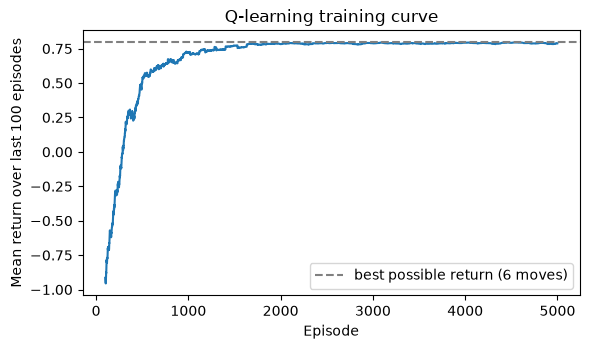
\includegraphics[width=.88\linewidth,height=5cm,keepaspectratio]{labs/visuals/06-notebook-reference.png}
\end{labvisual}

\textbf{What it means.} The first 100 episodes average a return of $-0.914$, and the last 100 average 0.788. That is just under the best possible 0.80, because 5\% of moves are still random.
\end{labanswer}

\begin{labquestion}{5}{Evaluate the greedy policy}
Training returns mix learning with random moves, so they are not a fair measure of the policy. Evaluation switches exploration off and follows the greedy policy: in each cell, take the action with the highest Q-value.
\end{labquestion}
\begin{labanswer}
\lstinputlisting[style=utppython,firstline=79,lastline=92]{all_experiments/lab06_reinforcement_worked.py}
\begin{refoutput}
\begin{lstlisting}[style=utpterminal]
success rate: 1.0
mean return: 0.8
learned action at start: down
\end{lstlisting}
\end{refoutput}

\textbf{What it means.} The goal is reached 200 times out of 200, with the best possible return. A mean of exactly 0.8 means the agent found a six-move route and never deviates from it.
\end{labanswer}

\textbf{Connect it to the chapter.} You have now run this loop 5,000 times.
% Reused from chapters/19-reinforcement-learning.tex
\begin{labvisual}{Recall the chapter model}
\begin{labgraphic}
\begin{tikzpicture}[
  node distance=3.5cm,
  box/.style={draw=UTPBlue,fill=UTPPaleBlue,rounded corners=2mm,minimum width=3cm,minimum height=1.2cm,align=center,font=\bfseries\color{UTPNavy}},
  arr/.style={-{Stealth[length=2.4mm]},thick,draw=UTPTeal}
]
\node[box] (agent) {Agent\\chooses an action};
\node[box,right=of agent] (env) {Environment\\changes state};
\draw[arr] (agent.north east) to[bend left=18] node[above,font=\small]{action $a_t$} (env.north west);
\draw[arr] (env.south west) to[bend left=18] node[below,font=\small]{state $s_{t+1}$, reward $r_{t+1}$} (agent.south east);
\end{tikzpicture}
\end{labgraphic}\end{labvisual}


\labpart{Part B --- The Q-table is the model: save it and read the policy}

\begin{labquestion}{6}{Save the table and read the policy}
Everything the agent learned is in the Q-table, so saving it is saving the model. Anyone with the file can act without retraining: in each cell, pick the action with the largest value.
\end{labquestion}
\begin{labanswer}
\lstinputlisting[style=utppython,firstline=94,lastline=103]{all_experiments/lab06_reinforcement_worked.py}
\begin{refoutput}
\begin{lstlisting}[style=utpterminal]
[['down' 'down' 'down' 'left']
 ['down' 'down' 'down' 'TRAP']
 ['right' 'down' 'down' 'down']
 ['right' 'right' 'right' 'GOAL']]
\end{lstlisting}
\end{refoutput}

\textbf{What it means.} From the start the route is down, down, right, down, right, right: six moves. A shortest route is not unique on a grid, so a different seed may pick another of the same length. The file is 640 bytes.
\end{labanswer}

\begin{labquestion}{7}{Draw the policy and the values}
The policy is easier to read as arrows on the grid, drawn over a heat map of each cell's value (the best Q-value available there). Values rise towards the goal.
\end{labquestion}
\begin{labanswer}
\lstinputlisting[style=utppython,firstline=105,lastline=126]{all_experiments/lab06_reinforcement_worked.py}
\begin{refoutput}
\begin{lstlisting}[style=utpterminal]
Best value in each cell (Q.max(axis=2)):
0.593  0.666  0.743  0.666
0.666  0.743  0.824  0.000
0.743  0.824  0.910  1.000
0.824  0.910  1.000  0.000
\end{lstlisting}
\end{refoutput}

\textbf{What it means.} These equal the exact values in \figref{fig:grid-values}, computed there without any trial and error. The agent learned them from rewards alone. The cell above the trap is worth 0.666, less than its left neighbor's 0.743, because the way out from there starts by stepping back left. The goal and trap cells are zero because no action is ever taken from them.
\end{labanswer}

\labpart{Evidence}

\begin{labquestion}{8}{Save the evidence}
Write the numbers above to the results folder. These files are regenerated on every run, so do not edit them by hand.
\end{labquestion}
\begin{labanswer}
\lstinputlisting[style=utppython,firstline=128,lastline=136]{all_experiments/lab06_reinforcement_worked.py}
\begin{refoutput}
\begin{lstlisting}[style=utpterminal]
Saved: ['greedy_policy.csv', 'greedy_policy_and_state_values.png', 'metrics.csv',
 'q_learning_training_curve.png', 'training_returns.csv', 'trap_moved_to_3_1.png']
\end{lstlisting}
\end{refoutput}
\end{labanswer}

\labpart{Try it yourself}

\begin{labquestion}{9}{Try it yourself}
Change one thing: the step cost, the trap location, the exploration schedule, or the discount factor. Write down what you expect the greedy policy to do differently before retraining, then check with \texttt{plot\_policy}. Attempt it in this empty cell before reading the solution.
\end{labquestion}

\begin{labquestion}{10}{One solution}
Move the trap onto the bottom row, at (3, 1). Prediction before retraining: the learned route runs through (3, 1), straight into the new trap, so the route has to change, for the same six-move length.
\end{labquestion}
\begin{labanswer}
\lstinputlisting[style=utppython,firstline=140,lastline=172]{all_experiments/lab06_reinforcement_worked.py}
\begin{refoutput}
\begin{lstlisting}[style=utpterminal]
Greedy policy with the trap at (3, 1):
down   down   right  down
right  down   down   down
right  right  right  down
up     TRAP   right  GOAL
\end{lstlisting}
\end{refoutput}

\textbf{What it means.} The route is now down, right, down, right, right, down: still six moves, so the return is still 0.8. The cell beside the new trap, (3, 0), points up and away from it. The right-hand column, which the original policy avoided, is now safe, and its arrows point down. The agent was never told the trap had moved; it relearned from the rewards alone.
\end{labanswer}

\begin{yourturn}
Add new cells at the end of the notebook for these tasks, using \texttt{train\_q} as a starting point. Write your prediction first, then run it.
\begin{enumerate}
  \item \textbf{No step cost.} Retrain with a step cost of 0. With no charge per move, does the agent still take a short route? Why, or why not?
  \item \textbf{A high step cost.} Retrain with a step cost of $-0.5$. Does the route change? What is its return?
  \item \textbf{Never explore.} Set $\varepsilon$ to 0 from the start. Predict whether the agent finds the goal. Then explain the result, thinking about what a $-0.04$ reward does to a Q-table that starts at zero.
  \item \textbf{Always explore.} Keep $\varepsilon$ at 1 throughout, so every training move is random. Does the \emph{greedy} policy read from the table still work?
\end{enumerate}
\end{yourturn}

\begin{expectedfindings}
\begin{enumerate}
  \item It still takes six moves, with a return of 1.00. With $\gamma=0.95$ a goal reached later is worth less, so the discount alone favors the short route.
  \item Still six moves, with a return of $5\times(-0.5)+1=-1.50$. Six moves is already the minimum, and the trap costs $-1$ at once, so the costly route is still best from the start.
  \item It reaches the goal in six moves with a return of 0.80, which may surprise you. Every tried action soon has a negative Q-value while untried ones stay at 0, so the greedy agent keeps trying whatever it has not tried. Starting at zero with negative step costs is accidental optimistic initialization. The food-stall student in Chapter~\ref{ch:rl} had no such luck, because every meal there could pay.
  \item Yes: six moves and a return of 0.80. Q-learning's backup uses the \emph{best} next action, whatever the agent actually did next, so it can learn the greedy policy's values while behaving randomly. Training returns would look terrible throughout, which is another reason to evaluate separately.
\end{enumerate}
\end{expectedfindings}

\begin{troubleshoot}
\begin{description}
  \item[The route differs from the sheet] Check whether you ran cells out of order: \texttt{rng} is shared, so rerunning a cell continues the random stream. Restart and run all. Any six-move route with return 0.8 is equally correct.
  \item[Return far below 0.8 in evaluation] Check that evaluation passes \texttt{explore=False}, and that you are not evaluating a half-trained table.
  \item[Arrows look upside down] \texttt{plt.imshow} puts row 0 at the top, so $y$ grows downward on this plot, which is why the code draws $-0.3\,dy$. Keep that sign.
  \item[The trap label is in the wrong place after the Try-it] The solution restores \texttt{TRAP} at the end of its cell. If you stopped midway, reset it to \texttt{(1, 3)}.
\end{description}
\end{troubleshoot}

\begin{labchecklists}
\begin{verification}
\begin{itemize}
  \item The greedy policy reaches the goal in six moves, for a return of $0.80$, and you can read that route from the printed policy.
  \item The success rate is reported over episodes run without exploration.
  \item \texttt{models/gridworld\_q\_table.npy} is saved, and the policy is read from the reloaded table.
  \item The first row of values matches 0.593, 0.666, 0.743, 0.666, and you can explain why the last is lower than the one before it.
\end{itemize}
\end{verification}

\begin{labdeliverable}
\begin{itemize}
  \item Restart the kernel and run all cells without errors.
  \item Submit the executed notebook, including your \emph{Your turn} cells, the generated \texttt{results/lab06/} folder, and the saved Q-table.
  \item Add a short conclusion: what you changed, what you predicted, what happened, and how the training curve differs from the greedy evaluation.
\end{itemize}
\end{labdeliverable}
\end{labchecklists}


\chapter{Neural Networks, CNNs, and Sequence Models}
\label{ch:deep}

\chapterguide%
  {Logistic regression from \chapref{ch:classification}, gradient descent from \chapref{ch:learning}, overfitting and validation from \chapref{ch:training}.}
  {run a small network forward by hand; solve XOR with two ReLU units; compute one backward pass and check it by nudging; count a network's weights; slide a filter over an image; explain what memory does in a recurrent network; and validate a network against simpler baselines.}

Logistic regression is one dimmer switch: a weighted sum, then a squash. A neural network is many of them wired together, so that the output of one becomes an input to the next. Nothing about the recipe changes. The model is richer, the loss is one you already know, and the optimizer is the same walk downhill. The new part is working out the slope for thousands of weights at once, and it turns out to be the chain rule, applied carefully.

\section{From logistic regression to a neural network}

A \term{layer} computes weighted sums, passes each through a nonlinear \term{activation}, and hands the results onward. The last layer has a sigmoid or softmax for classification, and a plain linear output for regression.

\begin{utpfig}[A feed-forward neural network]{A feed-forward network. Each hidden unit computes a weighted sum of the previous layer and passes it through a ReLU; the output layer produces the prediction.}{fig:mlp}
\begin{tikzpicture}[
  n/.style={circle,draw=UTPBlue,fill=UTPPaleBlue,minimum size=6.5mm,inner sep=0pt,font=\scriptsize\color{UTPNavy}},
  h/.style={circle,draw=UTPTeal,fill=UTPPaleTeal,minimum size=6.5mm,inner sep=0pt,font=\scriptsize\color{UTPNavy}},
  o/.style={circle,draw=UTPOrange,fill=UTPPaleOrange,minimum size=6.5mm,inner sep=0pt,font=\scriptsize\color{UTPNavy}},
  e/.style={draw=UTPMuted!55,thin}
]
\foreach \i/\y in {1/1.6,2/0.8,3/0,4/-0.8} \node[n] (x\i) at (0,\y) {$x_\i$};
\foreach \j/\y in {1/1.6,2/0.8,3/0,4/-0.8,5/-1.6} \node[h] (h\j) at (2.6,\y) {};
\foreach \k/\y in {1/0.8,2/0,3/-0.8} \node[h] (g\k) at (5.2,\y) {};
\node[o] (out) at (7.8,0) {$\hat{y}$};
\foreach \i in {1,...,4} \foreach \j in {1,...,5} \draw[e] (x\i) -- (h\j);
\foreach \j in {1,...,5} \foreach \k in {1,...,3} \draw[e] (h\j) -- (g\k);
\foreach \k in {1,...,3} \draw[e] (g\k) -- (out);
\node[font=\scriptsize\color{UTPMuted}] at (0,-1.6) {inputs};
\node[font=\scriptsize\color{UTPMuted},align=center] at (2.6,-2.4) {hidden layer 1\\(5 weighted sums, each\\passed through ReLU)};
\node[font=\scriptsize\color{UTPMuted}] at (5.2,-1.6) {hidden layer 2};
\node[font=\scriptsize\color{UTPMuted}] at (7.8,-1.0) {output};
\end{tikzpicture}
\end{utpfig}

\term{ReLU}, $\max(0,z)$, keeps positive inputs and zeroes negative ones. Think of it as a one-way valve. It is a very small amount of nonlinearity, and it is enough.

\begin{workedexample}
\textbf{One forward pass.} Take inputs $x=(2,1)$, a hidden layer with two units, weights $w_1=(1,-1)$ and $w_2=(0.5,0.5)$, no biases, and ReLU. The two sums are $2-1=1$ and $1+0.5=1.5$, and ReLU leaves both as they are. An output unit with weights $(1,-2)$ then gives $1-3=-2$, which a sigmoid turns into a chance of 0.119. Change $x$ to $(1,2)$: the first sum becomes $-1$, ReLU sets it to 0, and the output becomes $0-3=-3$.
\end{workedexample}

\subsection{Why hidden layers matter: XOR}

Without nonlinear activations, stacked linear layers collapse into one linear map, however many there are. Here is a problem that shows why that matters.

\begin{workedexample}
XOR is 1 when exactly one of two inputs is 1. The best possible straight-line fit predicts 0.5 for all four cases, so it has learned nothing.

Now use two ReLU units, $h_1=\max(0,x_1-x_2)$ and $h_2=\max(0,x_2-x_1)$, and output $h_1+h_2$.

\medskip
\centering\small
\begin{tabular}{@{}cccccc@{}}
\toprule
\rowcolor{UTPPaleBlue!92}
\utpth{$x_1$} & \utpth{$x_2$} & \utpth{$h_1$} & \utpth{$h_2$} & \utpth{Output} & \utpth{Target} \\
\midrule
0 & 0 & 0 & 0 & 0 & 0 \\
1 & 0 & 1 & 0 & 1 & 1 \\
0 & 1 & 0 & 1 & 1 & 1 \\
1 & 1 & 0 & 0 & 0 & 0 \\
\bottomrule
\end{tabular}
\par\raggedright
\medskip
The hidden units built new features, ``first but not second'' and ``second but not first'', and a straight line on those features solves it. Training finds such features instead of having them written by hand.
\end{workedexample}

\begin{intuition}
Hidden units create nonlinear features; later layers combine them into richer decision boundaries.
\end{intuition}

\section{How a network is trained}

Train by gradient-based optimization (\secref{sec:gradient-descent}):

\begin{utpsteps}
  \item \term{Forward pass.} Predict a minibatch and compute classification cross-entropy or regression squared loss.
  \item \term{Backward pass.} Backpropagation applies the chain rule to compute every weight's gradient.
  \item \term{Update.} An optimizer uses those gradients; the learning rate controls step size. The labs use Adam.
  \item \term{Repeat.} One pass through training batches is an \term{epoch}. Record validation performance each epoch.
\end{utpsteps}

\subsection{One backward pass by hand}

\term{Backpropagation} sounds grand, and it is the chain rule, used from the output backward so that each weight's slope reuses work already done.

\begin{workedexample}
A two-weight network: input $x=1$, hidden $h=\operatorname{ReLU}(a\,x)$, output $\hat{y}=b\,h$, target $y=2$, loss $(y-\hat{y})^2$. Start with $a=2$ and $b=0.5$.

\emph{Forward:} $h=2$, $\hat{y}=1$, loss $=1$.

\emph{Backward:} the error's slope with respect to $\hat{y}$ is $-2(y-\hat{y})=-2$. Moving back one step, $\hat{y}$ changes with $b$ at the rate $h=2$, so $\partial L/\partial b=-2\times2=-4$. Moving back again, $\hat{y}$ changes with $h$ at the rate $b=0.5$ and $h$ with $a$ at the rate $x=1$, so $\partial L/\partial a=-2\times0.5\times1=-1$.

\emph{Check by nudging:} changing $a$ by 0.00001 changes the loss at a rate of $-1.000$, and $b$ at a rate of $-4.000$. The chain rule is right.

\emph{Step} with a learning rate of 0.1: $a=2.1$ and $b=0.9$. Now $\hat{y}=1.89$ and the loss is 0.0121, down from 1.
\end{workedexample}

\begin{utptable}
\begin{tabularx}{\linewidth}{@{}>{\bfseries\leavevmode\color{UTPNavy}\ttfamily}m{0.2\linewidth}m{0.18\linewidth}X@{}}
\toprule
\rowcolor{UTPPaleBlue!92}
\utpth{Setting} & \utpth{Typical value} & \utpth{What raising it does} \\
\midrule
learning rate & 0.001--0.01 & Bigger steps: faster at first, unstable if too big \\
batch size & 32--128 & Smoother gradients, fewer updates per epoch \\
epochs & 10--50 & More passes; watch validation, not training \\
hidden units & 32--256 & More capacity; more risk of memorising \\
dropout & 0.1--0.5 & Randomly silences units during training; a regularizer \\
\bottomrule
\end{tabularx}
\end{utptable}

Monitor overfitting (\chapref{ch:training}). \term{Early stopping} retains the best validation weights; \term{dropout} randomly disables units during training.

\begin{keyidea}
Extra capacity makes validation and a one-time final test more important, not less.
\end{keyidea}

\begin{pitfall}
Scale inputs before training and save any training-fitted scaling statistics.
\end{pitfall}

\subsection{Counting weights}

Each dense layer has one weight per input per unit, plus one bias per unit. Lab~7's dense network, for $32\times32$ colour images, has $(3{,}072\times128+128)+(128\times7+7)=394{,}247$ weights.

\recipecard{Neural network}{Layers of weighted sums and nonlinear activations, with many thousands of weights.}{Cross-entropy for classes; squared error for numbers.}{Gradient descent on minibatches, usually with Adam. Backpropagation computes the slopes.}

\section{Convolutional networks for images}

\begin{analogy}
Lay a small stencil on a photo and slide it across, recording at each position how well the patch beneath matches the stencil. Wherever the pattern appears, the score is high. A \term{convolutional layer} does exactly this, except that it learns its own stencils, called \term{filters}. Each filter's scores form a \term{feature map}.
\end{analogy}

\begin{workedexample}
A $5\times5$ image, dark on the left and bright on the right, and a $3\times3$ vertical-edge filter. Each output is the sum of the filter times the patch beneath it.

\medskip
\centering
\begin{tikzpicture}
\foreach \r/\row in {0/{0,0,0,9,9},1/{0,0,0,9,9},2/{0,0,0,9,9},3/{0,0,0,9,9},4/{0,0,0,9,9}}
  \foreach \v [count=\c from 0] in \row
    \node[hcell,fill=UTPBlue!\v!white] at (\c*0.62,-\r*0.62) {\v};
\foreach \r in {0,1,2} \foreach \c/\v in {0/-1,1/0,2/1}
    \node[hkey] at (4.1+\c*0.62,-0.62-\r*0.62) {$\v$};
\foreach \r in {0,1,2} \foreach \c/\v in {0/0,1/27,2/27}
    \node[hhot] at (7.4+\c*0.62,-0.62-\r*0.62) {\v};
\node[utplabel,anchor=south] at (1.24,0.32) {image};
\node[utplabel,anchor=south] at (4.72,-0.28) {filter};
\node[utplabel,anchor=south] at (8.02,-0.28) {feature map};
\node[font=\Large\color{UTPMuted}] at (3.45,-1.24) {$*$};
\node[font=\Large\color{UTPMuted}] at (6.75,-1.24) {$=$};
\end{tikzpicture}
\par\raggedright
\medskip
The top-left output covers columns 0 to 2: left column $-1\times(0+0+0)$, right column $+1\times(0+0+0)$, so 0. One position to the right, the patch's right column is $9,9,9$, so the output is 27. The map is bright exactly where the edge lies. A horizontal-edge filter gives all zeros on this image, because it has no horizontal edge.
\end{workedexample}

\begin{utpfig}[A convolutional filter]{One $3\times3$ filter slides across an $8\times8$ image of a vertical stroke. With padding, the feature map is $8\times8$ too. It is positive (teal) where the stroke begins, negative (orange) where it ends, and strongest where the filter's whole height lies along the stroke. The blue square marks the filter's current position and the output it produces.}{fig:conv-filter}
\begin{tikzpicture}[font=\scriptsize]
\foreach \i in {1,...,6} \foreach \j in {3,4} \fill[UTPNavy!70] (\j*0.4,-\i*0.4) rectangle ++(0.4,-0.4);
\foreach \i in {0,...,7} \foreach \j in {0,...,7} \draw[UTPMuted!50] (\j*0.4,-\i*0.4) rectangle ++(0.4,-0.4);
\draw[UTPBlue,very thick] (0.4,-0.8) rectangle (1.6,-2.0);
\node[font=\small\bfseries\color{UTPNavy}] at (1.6,0.3) {image $8\times8$};
\begin{scope}[xshift=4.3cm,yshift=-0.85cm]
\foreach \i in {0,...,2} \foreach \j in {0,...,2} \draw[UTPMuted!60] (\j*0.5,-\i*0.5) rectangle ++(0.5,-0.5);
\foreach \i in {0,...,2} {
  \node at (0.25,-0.25-\i*0.5) {$-1$};
  \node at (0.75,-0.25-\i*0.5) {$0$};
  \node at (1.25,-0.25-\i*0.5) {$1$};
}
\node[font=\small\bfseries\color{UTPNavy}] at (0.75,0.35) {one filter};
\node[color=UTPMuted,align=center] at (0.75,-2.05) {it responds to\\vertical edges};
\end{scope}
\begin{scope}[xshift=7.3cm]
\foreach \i/\n in {0/1,1/2,2/3,3/3,4/3,5/3,6/2,7/1} {
  \pgfmathtruncatemacro{\shade}{\n*25}
  \foreach \j in {2,3} \fill[UTPTeal!\shade] (\j*0.4,-\i*0.4) rectangle ++(0.4,-0.4);
  \foreach \j in {4,5} \fill[UTPOrange!\shade] (\j*0.4,-\i*0.4) rectangle ++(0.4,-0.4);
}
\foreach \i in {0,...,7} \foreach \j in {0,...,7} \draw[UTPMuted!50] (\j*0.4,-\i*0.4) rectangle ++(0.4,-0.4);
\draw[UTPBlue,very thick] (0.8,-1.2) rectangle ++(0.4,-0.4);
\node[font=\small\bfseries\color{UTPNavy}] at (1.6,0.3) {feature map};
\end{scope}
\draw[-{Stealth[length=2mm]},UTPBlue,thick] (3.3,-1.6) -- (4.2,-1.6);
\draw[-{Stealth[length=2mm]},UTPBlue,thick] (5.9,-1.6) -- (7.2,-1.6);
\end{tikzpicture}
\end{utpfig}

Filters share weights across locations: the same few numbers slide everywhere, so a stroke found in one corner is found in every corner, and the layer needs far fewer weights than a dense one. \term{Max pooling} keeps the largest value in each block, which shrinks the map while keeping what fired. Pooling the $4\times4$ map with rows $1,3,2,0$; $4,2,0,1$; $0,0,5,6$; $1,2,3,0$ into $2\times2$ blocks gives $4,2$ and $2,6$. A small CNN repeats convolution, ReLU and pooling, then flattens the maps into a dense classifier.

\keepspace{20\baselineskip}
\begin{workedexample}
Lab~7's CNN for $32\times32$ colour photos of wood defects, with weights counted per layer. A filter layer has (input channels $\times$ filters $\times$ $3\times3$) weights plus one bias per filter, and a colour image has three input channels. The two filter layers need 5,088 weights between them, the first dense layer 131,136, which is why the pooling before it matters.

\medskip
\centering\small
\begin{tabular}{@{}lcc@{}}
\toprule
\rowcolor{UTPPaleBlue!92}
\utpth{Layer} & \utpth{Output shape} & \utpth{Weights} \\
\midrule
Input & $3\times32\times32$ & \\
Conv, 16 filters, then pool & $16\times16\times16$ & $3\times16\times9+16=448$ \\
Conv, 32 filters, then pool & $32\times8\times8$ & $16\times32\times9+32=4{,}640$ \\
Flatten & 2,048 & \\
Dense, 64 units & 64 & $2{,}048\times64+64=131{,}136$ \\
Dense, 7 classes & 7 & $64\times7+7=455$ \\
\midrule
Total & & 136,679 \\
\bottomrule
\end{tabular}
\end{workedexample}

\begin{intuition}
Training learns filters that reduce loss, rather than relying on hand-specified edges or shapes.
\end{intuition}

\section{Sequence models: RNNs and LSTMs}

\begin{analogy}
Reading a sentence, you do not start afresh at each word: you carry a running sense of what has happened so far. A \term{recurrent network} carries a \term{hidden state} in the same way, like a reader keeping a small notepad. Each step combines the new input with the notes so far and writes new notes.
\end{analogy}

\begin{workedexample}
A toy recurrent unit with fixed weights: $\text{state}=0.5\times\text{previous state}+\text{input}$. Inputs $1,2,3$ give states $1,\ 2.5,\ 4.25$. The final state holds all three inputs, with the oldest counting least.

That fading is also the weakness. At 0.5 per step, an input's weight after 8 steps is 0.0039, and after 24 steps it is about 0.00000006. A plain network has trouble remembering yesterday by the time it reaches today.
\end{workedexample}

\begin{utpfig}[An LSTM unrolled over a window]{An LSTM unrolled over a 24-hour window. Each step combines the new input with the state passed from the previous step, and the final state supports the prediction.}{fig:lstm-unrolled}
\begin{tikzpicture}[
  cell/.style={draw=UTPTeal,fill=UTPPaleTeal,rounded corners=1.5mm,minimum width=1.5cm,minimum height=0.9cm,font=\scriptsize\bfseries\color{UTPNavy}},
  inp/.style={draw=UTPBlue,fill=UTPPaleBlue,rounded corners=1.2mm,minimum width=1.2cm,minimum height=0.6cm,font=\scriptsize\color{UTPNavy}},
  outp/.style={draw=UTPOrange,fill=UTPPaleOrange,rounded corners=1.2mm,minimum width=1.5cm,minimum height=0.6cm,font=\scriptsize\color{UTPNavy}},
  arr/.style={-{Stealth[length=1.8mm]},thick,draw=UTPTeal}
]
\foreach \t/\x in {1/0,2/2.4,3/4.8,24/8.4} {
  \node[cell] (c\t) at (\x,0) {LSTM};
  \node[inp] (i\t) at (\x,-1.4) {$x_{\t}$};
  \draw[arr] (i\t) -- (c\t);
}
\node[font=\Large\color{UTPMuted}] at (6.6,0) {$\cdots$};
\draw[arr] (c1) -- node[above,font=\scriptsize\color{UTPMuted}] {state} (c2);
\draw[arr] (c2) -- node[above,font=\scriptsize\color{UTPMuted}] {state} (c3);
\draw[arr] (c3) -- (6.1,0);
\draw[arr] (7.1,0) -- (c24);
\node[outp] (o) at (8.4,1.5) {$\hat{y}_{25}$};
\draw[arr] (c24) -- (o);
\node[font=\scriptsize\color{UTPMuted},align=center] at (4.2,-2.3) {24 hourly demand values go in, one step at a time; the same cell (same weights) is used at every step;\\the final state predicts the next hour};
\end{tikzpicture}
\end{utpfig}

An \term{LSTM} adds a second notepad, the memory cell, and three learned gates that control it: what to erase, what to write, and what to read out. Because the cell is updated by adding rather than repeatedly shrinking, information can survive many steps. With a keep gate of 0.8 on a note of 10, and a write gate of 0.5 on a new value of 4, the note becomes $0.8\times10+0.5\times4=10$. The gates' values come from small learned networks, so the model decides for itself what is worth keeping.

\begin{workedexample}
From series to windows. A sequence model does not take a table of features; it takes the last few values and predicts the next. With lookback 3, the series $16,40,32,13,1,1,2,3$ gives five rows:

\medskip
\centering\small
\begin{tabular}{@{}cc@{}}
\toprule
\rowcolor{UTPPaleBlue!92}
\utpth{Input window} & \utpth{Target} \\
\midrule
16, 40, 32 & 13 \\
40, 32, 13 & 1 \\
32, 13, 1 & 1 \\
13, 1, 1 & 2 \\
1, 1, 2 & 3 \\
\bottomrule
\end{tabular}
\par\raggedright
\medskip
$N$ values give $N$ minus lookback windows. Neighboring rows overlap, so a random split would put almost the same row on both sides: split in date order. The simplest forecast, \term{persistence}, says the next value equals the last, and on these targets its misses are 19, 12, 0, 1 and 1.
\end{workedexample}

Lab~8 predicts the next hour's electricity demand of 158 customers from the previous 24. Its network has $4\times(32+32\times32+32+32)=4{,}480$ LSTM weights plus 33 in the output layer, 4,513 in all. On the second half of 2014, persistence misses by 6.12~MWh in an average hour, ``same hour yesterday'' by 3.69, and the LSTM by 2.57, which is 2.4\% of the average hour.

\begin{pitfall}
Compare against last-value and same-hour-yesterday forecasts. Keep the network only if its validated gain justifies its cost.
\end{pitfall}

\section{Practical notes}

\begin{itemize}
  \item \term{Set the seed} (\texttt{torch.manual\_seed}) and expect small run-to-run differences anyway; training is stochastic.
  \item \term{Scale inputs} using training data only; save the fitted scaling.
  \item \term{Save weights} with \texttt{torch.save(model.state\_dict(), path)}. Include the architecture and model card needed to reload them.
  \item \term{Windows OpenMP conflicts:} duplicate runtimes may trigger ``OMP: Error \#15''. Check the environment setup before rerunning.
  \item \term{A CPU suffices} for these labs; larger workloads may benefit from a GPU.
  \item \term{Keep classical baselines.} Compare neural models with boosting on tables and simpler predictors on images or sequences.
\end{itemize}

\begin{modelcard}{Neural Networks - Quick Guide}
\begin{tabularx}{\linewidth}{@{}>{\bfseries\leavevmode\color{UTPNavy}}p{0.22\linewidth}X@{}}
Best when & Inputs are images, sequences, or text; there is plenty of data; useful features are hard to write by hand. \cr
Start with & A small dense network as the reference, then a CNN for grids or an LSTM for sequences; always beside a classical baseline. \cr
Preprocessing & Scale inputs to a small range using training data; window a time series; split chronologically when rows overlap in time. \cr
Main controls & Learning rate, epochs (with early stopping), batch size, layer sizes, dropout. \cr
Watch for & Memorising the training set, unscaled inputs, run-to-run variation, and a baseline that was never beaten. \cr
\end{tabularx}
\end{modelcard}

\begin{libnote}
Labs~7--8 use \lib{PyTorch} tensors, \texttt{nn.Sequential}, and explicit training loops. \lib{Keras} instead offers a higher-level \texttt{model.fit} interface.
\end{libnote}

\section{The whole map}

An hour's worth of names is now a map with a few corners, and every method in this book lives somewhere on it. When you meet a new name, do not try to memorize it. Ask which corner it lives in, and which step of the recipe it changes.

\begin{utptable}
\begin{tabularx}{\linewidth}{@{}>{\bfseries\leavevmode\color{UTPNavy}}m{0.21\linewidth}m{0.14\linewidth}X X X@{}}
\toprule
\rowcolor{UTPPaleBlue!92}
\utpth{Method} & \utpth{Corner} & \utpth{Model} & \utpth{Loss} & \utpth{Optimizer} \\
\midrule
Linear regression & Number & Line & Squared error & Exact formula \\
Logistic regression & Category & Line, squashed & Log loss & Gradient descent \\
$k$-NN & Either & Stored rows & None & None \\
Naive Bayes & Category & Prior times clues & Negative likelihood & Counting \\
Decision tree & Either & Questions & Gini or squared error & Greedy splits \\
Random forest & Either & Many deep trees & Same, per tree & Independent greedy fits \\
Gradient boosting & Either & Sum of shallow trees & Any differentiable loss & Sequential fits to the gradient \\
SVM & Either & Widest street & Hinge loss & Quadratic program \\
$K$-means & Groups & $K$ landmarks & Squared distance & Assign, move, repeat \\
PCA & Fewer columns & A few directions & Spread lost & Exact matrix routine \\
Q-learning & Rewards & Table of values & TD error & Small step per move \\
Neural network & Any & Layers & Task's loss & Backpropagation with gradient descent \\
\bottomrule
\end{tabularx}
\end{utptable}

\begin{keyidea}
Machine learning is one recipe with its parts swapped. Pick a formula with numbers you are allowed to change, measure its errors with one number, and find the values that make that number smaller. Then check the result on data it has not seen.
\end{keyidea}

\begin{chapterrecap}
\begin{itemize}
  \item A network wires dimmer switches together. Without nonlinear activations it collapses to one linear map, and with them it can solve XOR.
  \item Backpropagation is the chain rule from the output backward, and a nudge can check any slope.
  \item A CNN slides learned filters and shares their weights, so it needs fewer weights to find a pattern anywhere. Pooling shrinks the maps.
  \item A recurrent network carries a hidden state. An LSTM adds a memory cell with gates, so that older information can survive.
  \item Same workflow, same honesty: compare with simple baselines, split sequences in date order, and report the variation between runs.
\end{itemize}
\end{chapterrecap}

\begin{quickcheck}
\begin{enumerate}
  \item Why does a network with two linear layers and no activation function have no more power than one linear layer?
  \item For $x=(3,1)$ and the forward-pass network above, what are the hidden values and the output score?
  \item How many weights does a dense layer from 128 inputs to 64 units have?
  \item What does a convolutional filter share across the image, and why does that reduce the number of weights?
  \item What does a max-pooling layer do to an $8\times8$ map with block size 2, and why is that useful?
  \item Why must the rows built from a windowed time series be split chronologically rather than at random?
\end{enumerate}
\end{quickcheck}


\chapter*{Capstone Project: From Raw Data to Defensible Evidence}
\phantomsection
\addcontentsline{toc}{chapter}{Capstone Project}
\markboth{Capstone Project}{}

Build one reproducible project from raw data to validated conclusions and a reusable model. The labs handed you the question, the data and the code. Here you choose all three, and you defend every decision with evidence.

\begin{coursechoice}
Use a public dataset not used as a main lab dataset; Heart Failure is allowed, since it appears only in a Lab~2 task. Keep raw files in \texttt{all\_datasets/} and notebooks in \texttt{all\_experiments/}.
\end{coursechoice}

\section*{Before you start}

Write one page answering three questions, and show it to your tutor before modeling.

\begin{utpsteps}
  \item \textbf{Which corner of the map?} Does your log hold the answers? Do you want a number, a category, groups, or fewer columns (\figref{fig:ml-map})?
  \item \textbf{What decision does this serve?} Name who would use the output, and what each kind of wrong answer costs them.
  \item \textbf{When is the prediction made?} List the columns that exist at that moment. Everything else is leakage (\secref{sec:data-leakage}).
\end{utpsteps}

\section*{Required capstone sequence}

\begin{enumerate}
  \item \textbf{Problem.} Specify rows, objective, use moment, population, metric, and error costs.
  \item \textbf{Data.} Record provenance, schema, units, missingness, duplicates, invalid values, identifiers, and cleaning rules.
  \item \textbf{Splits.} Match future use with random, stratified, grouped, or chronological splits; reserve a supervised test set.
  \item \textbf{Baseline.} Evaluate a no-skill or domain rule.
  \item \textbf{Preprocessing.} Fit learned transformations within training folds.
  \item \textbf{Models.} Compare at least three families, including one interpretable model.
  \item \textbf{Development.} Tune, select features, and resample only within validated development pipelines.
  \item \textbf{Diagnostics.} Plot relevant errors, residuals, thresholds, learning curves, features, clusters, or scores.
  \item \textbf{Subgroups.} Locate failures beyond aggregate metrics.
  \item \textbf{Final evidence.} Test once on untouched supervised data, or present complementary unsupervised evidence.
  \item \textbf{Limits.} Distinguish prediction from causation and state unsupported claims.
  \item \textbf{Reproducibility.} Record paths, packages, seeds, notebook order, and configuration.
  \item \textbf{Artifact.} Save the pipeline and model card under \texttt{models/}; demonstrate reloading and prediction.
\end{enumerate}

\section*{What to hand in}

\begin{labdeliverable}
\begin{itemize}
  \item A notebook that runs from top to bottom after \textbf{Restart Kernel and Run All Cells}.
  \item The saved pipeline and model card under \texttt{models/}, with a cell that reloads them and predicts one new row.
  \item A results table: baseline, each model family, and the locked model's one test score.
  \item A two-page report in your own words: the problem and its costs, the split and why it imitates real use, what you compared, what you chose and why, where the model fails, and what it must not be used for.
\end{itemize}
\end{labdeliverable}

\section*{How it is judged}

\begin{utptable}
\begin{tabularx}{\linewidth}{@{}>{\bfseries\leavevmode\color{UTPNavy}}m{0.24\linewidth}X@{}}
\toprule
\rowcolor{UTPPaleBlue!92}
\utpth{Criterion} & \utpth{What good looks like} \\
\midrule
Honest evaluation & The split imitates real use, preprocessing sits inside a pipeline, and the test set is opened once. \\
Baseline & Every model is compared with a rule that costs nothing, on the same rows. \\
Comparison & Three families under one protocol, with fold spread or another estimate of uncertainty. \\
Diagnosis & At least one look at actual errors or subgroups, and what it changed. \\
Reasoning & Each choice is justified by evidence, including choosing a simpler model when a gain is within noise. \\
Reproducibility & Someone else can rerun it and get your numbers, and your report states what may vary. \\
\bottomrule
\end{tabularx}
\end{utptable}

\begin{pitfall}
Three mistakes cost the most. Fitting a scaler or selector on all the rows before cross-validating. Reporting the best of many test scores. Claiming a cause from a coefficient or an importance score. The course gave you a tool to avoid each one.
\end{pitfall}


\end{document}
